% Options for packages loaded elsewhere
% Options for packages loaded elsewhere
\PassOptionsToPackage{unicode}{hyperref}
\PassOptionsToPackage{hyphens}{url}
\PassOptionsToPackage{dvipsnames,svgnames,x11names}{xcolor}
%
\documentclass[
  letterpaper,
  DIV=11,
  numbers=noendperiod]{scrreprt}
\usepackage{xcolor}
\usepackage{amsmath,amssymb}
\setcounter{secnumdepth}{-\maxdimen} % remove section numbering
\usepackage{iftex}
\ifPDFTeX
  \usepackage[T1]{fontenc}
  \usepackage[utf8]{inputenc}
  \usepackage{textcomp} % provide euro and other symbols
\else % if luatex or xetex
  \usepackage{unicode-math} % this also loads fontspec
  \defaultfontfeatures{Scale=MatchLowercase}
  \defaultfontfeatures[\rmfamily]{Ligatures=TeX,Scale=1}
\fi
\usepackage{lmodern}
\ifPDFTeX\else
  % xetex/luatex font selection
\fi
% Use upquote if available, for straight quotes in verbatim environments
\IfFileExists{upquote.sty}{\usepackage{upquote}}{}
\IfFileExists{microtype.sty}{% use microtype if available
  \usepackage[]{microtype}
  \UseMicrotypeSet[protrusion]{basicmath} % disable protrusion for tt fonts
}{}
\makeatletter
\@ifundefined{KOMAClassName}{% if non-KOMA class
  \IfFileExists{parskip.sty}{%
    \usepackage{parskip}
  }{% else
    \setlength{\parindent}{0pt}
    \setlength{\parskip}{6pt plus 2pt minus 1pt}}
}{% if KOMA class
  \KOMAoptions{parskip=half}}
\makeatother
% Make \paragraph and \subparagraph free-standing
\makeatletter
\ifx\paragraph\undefined\else
  \let\oldparagraph\paragraph
  \renewcommand{\paragraph}{
    \@ifstar
      \xxxParagraphStar
      \xxxParagraphNoStar
  }
  \newcommand{\xxxParagraphStar}[1]{\oldparagraph*{#1}\mbox{}}
  \newcommand{\xxxParagraphNoStar}[1]{\oldparagraph{#1}\mbox{}}
\fi
\ifx\subparagraph\undefined\else
  \let\oldsubparagraph\subparagraph
  \renewcommand{\subparagraph}{
    \@ifstar
      \xxxSubParagraphStar
      \xxxSubParagraphNoStar
  }
  \newcommand{\xxxSubParagraphStar}[1]{\oldsubparagraph*{#1}\mbox{}}
  \newcommand{\xxxSubParagraphNoStar}[1]{\oldsubparagraph{#1}\mbox{}}
\fi
\makeatother

\usepackage{color}
\usepackage{fancyvrb}
\newcommand{\VerbBar}{|}
\newcommand{\VERB}{\Verb[commandchars=\\\{\}]}
\DefineVerbatimEnvironment{Highlighting}{Verbatim}{commandchars=\\\{\}}
% Add ',fontsize=\small' for more characters per line
\usepackage{framed}
\definecolor{shadecolor}{RGB}{241,243,245}
\newenvironment{Shaded}{\begin{snugshade}}{\end{snugshade}}
\newcommand{\AlertTok}[1]{\textcolor[rgb]{0.68,0.00,0.00}{#1}}
\newcommand{\AnnotationTok}[1]{\textcolor[rgb]{0.37,0.37,0.37}{#1}}
\newcommand{\AttributeTok}[1]{\textcolor[rgb]{0.40,0.45,0.13}{#1}}
\newcommand{\BaseNTok}[1]{\textcolor[rgb]{0.68,0.00,0.00}{#1}}
\newcommand{\BuiltInTok}[1]{\textcolor[rgb]{0.00,0.23,0.31}{#1}}
\newcommand{\CharTok}[1]{\textcolor[rgb]{0.13,0.47,0.30}{#1}}
\newcommand{\CommentTok}[1]{\textcolor[rgb]{0.37,0.37,0.37}{#1}}
\newcommand{\CommentVarTok}[1]{\textcolor[rgb]{0.37,0.37,0.37}{\textit{#1}}}
\newcommand{\ConstantTok}[1]{\textcolor[rgb]{0.56,0.35,0.01}{#1}}
\newcommand{\ControlFlowTok}[1]{\textcolor[rgb]{0.00,0.23,0.31}{\textbf{#1}}}
\newcommand{\DataTypeTok}[1]{\textcolor[rgb]{0.68,0.00,0.00}{#1}}
\newcommand{\DecValTok}[1]{\textcolor[rgb]{0.68,0.00,0.00}{#1}}
\newcommand{\DocumentationTok}[1]{\textcolor[rgb]{0.37,0.37,0.37}{\textit{#1}}}
\newcommand{\ErrorTok}[1]{\textcolor[rgb]{0.68,0.00,0.00}{#1}}
\newcommand{\ExtensionTok}[1]{\textcolor[rgb]{0.00,0.23,0.31}{#1}}
\newcommand{\FloatTok}[1]{\textcolor[rgb]{0.68,0.00,0.00}{#1}}
\newcommand{\FunctionTok}[1]{\textcolor[rgb]{0.28,0.35,0.67}{#1}}
\newcommand{\ImportTok}[1]{\textcolor[rgb]{0.00,0.46,0.62}{#1}}
\newcommand{\InformationTok}[1]{\textcolor[rgb]{0.37,0.37,0.37}{#1}}
\newcommand{\KeywordTok}[1]{\textcolor[rgb]{0.00,0.23,0.31}{\textbf{#1}}}
\newcommand{\NormalTok}[1]{\textcolor[rgb]{0.00,0.23,0.31}{#1}}
\newcommand{\OperatorTok}[1]{\textcolor[rgb]{0.37,0.37,0.37}{#1}}
\newcommand{\OtherTok}[1]{\textcolor[rgb]{0.00,0.23,0.31}{#1}}
\newcommand{\PreprocessorTok}[1]{\textcolor[rgb]{0.68,0.00,0.00}{#1}}
\newcommand{\RegionMarkerTok}[1]{\textcolor[rgb]{0.00,0.23,0.31}{#1}}
\newcommand{\SpecialCharTok}[1]{\textcolor[rgb]{0.37,0.37,0.37}{#1}}
\newcommand{\SpecialStringTok}[1]{\textcolor[rgb]{0.13,0.47,0.30}{#1}}
\newcommand{\StringTok}[1]{\textcolor[rgb]{0.13,0.47,0.30}{#1}}
\newcommand{\VariableTok}[1]{\textcolor[rgb]{0.07,0.07,0.07}{#1}}
\newcommand{\VerbatimStringTok}[1]{\textcolor[rgb]{0.13,0.47,0.30}{#1}}
\newcommand{\WarningTok}[1]{\textcolor[rgb]{0.37,0.37,0.37}{\textit{#1}}}

\usepackage{longtable,booktabs,array}
\usepackage{calc} % for calculating minipage widths
% Correct order of tables after \paragraph or \subparagraph
\usepackage{etoolbox}
\makeatletter
\patchcmd\longtable{\par}{\if@noskipsec\mbox{}\fi\par}{}{}
\makeatother
% Allow footnotes in longtable head/foot
\IfFileExists{footnotehyper.sty}{\usepackage{footnotehyper}}{\usepackage{footnote}}
\makesavenoteenv{longtable}
\usepackage{graphicx}
\makeatletter
\newsavebox\pandoc@box
\newcommand*\pandocbounded[1]{% scales image to fit in text height/width
  \sbox\pandoc@box{#1}%
  \Gscale@div\@tempa{\textheight}{\dimexpr\ht\pandoc@box+\dp\pandoc@box\relax}%
  \Gscale@div\@tempb{\linewidth}{\wd\pandoc@box}%
  \ifdim\@tempb\p@<\@tempa\p@\let\@tempa\@tempb\fi% select the smaller of both
  \ifdim\@tempa\p@<\p@\scalebox{\@tempa}{\usebox\pandoc@box}%
  \else\usebox{\pandoc@box}%
  \fi%
}
% Set default figure placement to htbp
\def\fps@figure{htbp}
\makeatother





\setlength{\emergencystretch}{3em} % prevent overfull lines

\providecommand{\tightlist}{%
  \setlength{\itemsep}{0pt}\setlength{\parskip}{0pt}}



 


\KOMAoption{captions}{tableheading}
\makeatletter
\@ifpackageloaded{bookmark}{}{\usepackage{bookmark}}
\makeatother
\makeatletter
\@ifpackageloaded{caption}{}{\usepackage{caption}}
\AtBeginDocument{%
\ifdefined\contentsname
  \renewcommand*\contentsname{Table of contents}
\else
  \newcommand\contentsname{Table of contents}
\fi
\ifdefined\listfigurename
  \renewcommand*\listfigurename{List of Figures}
\else
  \newcommand\listfigurename{List of Figures}
\fi
\ifdefined\listtablename
  \renewcommand*\listtablename{List of Tables}
\else
  \newcommand\listtablename{List of Tables}
\fi
\ifdefined\figurename
  \renewcommand*\figurename{Figure}
\else
  \newcommand\figurename{Figure}
\fi
\ifdefined\tablename
  \renewcommand*\tablename{Table}
\else
  \newcommand\tablename{Table}
\fi
}
\@ifpackageloaded{float}{}{\usepackage{float}}
\floatstyle{ruled}
\@ifundefined{c@chapter}{\newfloat{codelisting}{h}{lop}}{\newfloat{codelisting}{h}{lop}[chapter]}
\floatname{codelisting}{Listing}
\newcommand*\listoflistings{\listof{codelisting}{List of Listings}}
\makeatother
\makeatletter
\makeatother
\makeatletter
\@ifpackageloaded{caption}{}{\usepackage{caption}}
\@ifpackageloaded{subcaption}{}{\usepackage{subcaption}}
\makeatother
\usepackage{bookmark}
\IfFileExists{xurl.sty}{\usepackage{xurl}}{} % add URL line breaks if available
\urlstyle{same}
\hypersetup{
  pdftitle={The Little Book of Linear Algebra},
  pdfauthor={Duc-Tam Nguyen},
  colorlinks=true,
  linkcolor={blue},
  filecolor={Maroon},
  citecolor={Blue},
  urlcolor={Blue},
  pdfcreator={LaTeX via pandoc}}


\title{The Little Book of Linear Algebra}
\usepackage{etoolbox}
\makeatletter
\providecommand{\subtitle}[1]{% add subtitle to \maketitle
  \apptocmd{\@title}{\par {\large #1 \par}}{}{}
}
\makeatother
\subtitle{Version 0.3.0}
\author{Duc-Tam Nguyen}
\date{2025-09-26}
\begin{document}
\maketitle

\renewcommand*\contentsname{Table of contents}
{
\hypersetup{linkcolor=}
\setcounter{tocdepth}{2}
\tableofcontents
}

\bookmarksetup{startatroot}

\chapter{Content}\label{content}

\subsubsection{Chapter 1. Vectors, Scalars, and
Geometry}\label{chapter-1.-vectors-scalars-and-geometry}

\begin{enumerate}
\def\labelenumi{\arabic{enumi}.}
\tightlist
\item
  Scalars, vectors, and coordinate systems (what they are, why we care)
\item
  Vector notation, components, and arrows (reading and writing vectors)
\item
  Vector addition and scalar multiplication (the two basic moves)
\item
  Linear combinations and span (building new vectors from old ones)
\item
  Length (norm) and distance (how big and how far)
\item
  Dot product (algebraic and geometric views)
\item
  Angles between vectors and cosine (measuring alignment)
\item
  Projections and decompositions (splitting along a direction)
\item
  Cauchy--Schwarz and triangle inequalities (two fundamental bounds)
\item
  Orthonormal sets in ℝ²/ℝ³ (nice bases you already know)
\end{enumerate}

\subsubsection{Chapter 2. Matrices and Basic
Operations}\label{chapter-2.-matrices-and-basic-operations}

\begin{enumerate}
\def\labelenumi{\arabic{enumi}.}
\setcounter{enumi}{10}
\tightlist
\item
  Matrices as tables and as machines (two mental models)
\item
  Matrix shapes, indexing, and block views (seeing structure)
\item
  Matrix addition and scalar multiplication (componentwise rules)
\item
  Matrix--vector product (linear combos of columns)
\item
  Matrix--matrix product (composition of linear steps)
\item
  Identity, inverse, and transpose (three special friends)
\item
  Symmetric, diagonal, triangular, and permutation matrices (special
  families)
\item
  Trace and basic matrix properties (quick invariants)
\item
  Affine transforms and homogeneous coordinates (translations included)
\item
  Computing with matrices (cost counts and simple speedups)
\end{enumerate}

\subsubsection{Chapter 3. Linear Systems and
Elimination}\label{chapter-3.-linear-systems-and-elimination}

\begin{enumerate}
\def\labelenumi{\arabic{enumi}.}
\setcounter{enumi}{20}
\tightlist
\item
  From equations to matrices (augmenting and encoding)
\item
  Row operations (legal moves that keep solutions)
\item
  Row-echelon and reduced row-echelon forms (target shapes)
\item
  Pivots, free variables, and leading ones (reading solutions)
\item
  Solving consistent systems (unique vs.~infinite solutions)
\item
  Detecting inconsistency (when no solution exists)
\item
  Gaussian elimination by hand (a disciplined procedure)
\item
  Back substitution and solution sets (finishing cleanly)
\item
  Rank and its first meaning (pivots as information)
\item
  LU factorization (elimination captured as L and U)
\end{enumerate}

\subsubsection{Chapter 4. Vector Spaces and
Subspaces}\label{chapter-4.-vector-spaces-and-subspaces}

\begin{enumerate}
\def\labelenumi{\arabic{enumi}.}
\setcounter{enumi}{30}
\tightlist
\item
  Axioms of vector spaces (what ``space'' really means)
\item
  Subspaces, column space, and null space (where solutions live)
\item
  Span and generating sets (coverage of a space)
\item
  Linear independence and dependence (no redundancy vs.~redundancy)
\item
  Basis and coordinates (naming every vector uniquely)
\item
  Dimension (how many directions)
\item
  Rank--nullity theorem (dimensions that add up)
\item
  Coordinates relative to a basis (changing the ``ruler'')
\item
  Change-of-basis matrices (moving between coordinate systems)
\item
  Affine subspaces (lines and planes not through the origin)
\end{enumerate}

\subsubsection{Chapter 5. Linear Transformations and
Structure}\label{chapter-5.-linear-transformations-and-structure}

\begin{enumerate}
\def\labelenumi{\arabic{enumi}.}
\setcounter{enumi}{40}
\tightlist
\item
  Linear transformations (preserving lines and sums)
\item
  Matrix representation of a linear map (choosing a basis)
\item
  Kernel and image (inputs that vanish; outputs we can reach)
\item
  Invertibility and isomorphisms (perfectly reversible maps)
\item
  Composition, powers, and iteration (doing it again and again)
\item
  Similarity and conjugation (same action, different basis)
\item
  Projections and reflections (idempotent and involutive maps)
\item
  Rotations and shear (geometric intuition)
\item
  Rank and operator viewpoint (rank beyond elimination)
\item
  Block matrices and block maps (divide and conquer structure)
\end{enumerate}

\subsubsection{Chapter 6. Determinants and
Volume}\label{chapter-6.-determinants-and-volume}

\begin{enumerate}
\def\labelenumi{\arabic{enumi}.}
\setcounter{enumi}{50}
\tightlist
\item
  Areas, volumes, and signed scale factors (geometric entry point)
\item
  Determinant via linear rules (multilinearity, sign, normalization)
\item
  Determinant and row operations (how each move changes det)
\item
  Triangular matrices and product of diagonals (fast wins)
\item
  det(AB) = det(A)det(B) (multiplicative magic)
\item
  Invertibility and zero determinant (flat vs.~full volume)
\item
  Cofactor expansion (Laplace's method)
\item
  Permutations and sign (the combinatorial core)
\item
  Cramer's rule (solving with determinants, and when not to use it)
\item
  Computing determinants in practice (use LU, mind stability)
\end{enumerate}

\subsubsection{Chapter 7. Eigenvalues, Eigenvectors, and
Dynamics}\label{chapter-7.-eigenvalues-eigenvectors-and-dynamics}

\begin{enumerate}
\def\labelenumi{\arabic{enumi}.}
\setcounter{enumi}{60}
\tightlist
\item
  Eigenvalues and eigenvectors (directions that stay put)
\item
  Characteristic polynomial (where eigenvalues come from)
\item
  Algebraic vs.~geometric multiplicity (how many and how independent)
\item
  Diagonalization (when a matrix becomes simple)
\item
  Powers of a matrix (long-term behavior via eigenvalues)
\item
  Real vs.~complex spectra (rotations and oscillations)
\item
  Defective matrices and a peek at Jordan form (when diagonalization
  fails)
\item
  Stability and spectral radius (grow, decay, or oscillate)
\item
  Markov chains and steady states (probabilities as linear algebra)
\item
  Linear differential systems (solutions via eigen-decomposition)
\end{enumerate}

\subsubsection{Chapter 8. Orthogonality, Least Squares, and
QR}\label{chapter-8.-orthogonality-least-squares-and-qr}

\begin{enumerate}
\def\labelenumi{\arabic{enumi}.}
\setcounter{enumi}{70}
\tightlist
\item
  Inner products beyond dot product (custom notions of angle)
\item
  Orthogonality and orthonormal bases (perpendicular power)
\item
  Gram--Schmidt process (constructing orthonormal bases)
\item
  Orthogonal projections onto subspaces (closest point principle)
\item
  Least-squares problems (fit when exact solve is impossible)
\item
  Normal equations and geometry of residuals (why it works)
\item
  QR factorization (stable least squares via orthogonality)
\item
  Orthogonal matrices (length-preserving transforms)
\item
  Fourier viewpoint (expanding in orthogonal waves)
\item
  Polynomial and multifeature least squares (fitting more flexibly)
\end{enumerate}

\subsubsection{Chapter 9. SVD, PCA, and
Conditioning}\label{chapter-9.-svd-pca-and-conditioning}

\begin{enumerate}
\def\labelenumi{\arabic{enumi}.}
\setcounter{enumi}{80}
\tightlist
\item
  Singular values and SVD (universal factorization)
\item
  Geometry of SVD (rotations + stretching)
\item
  Relation to eigen-decompositions (ATA and AAT)
\item
  Low-rank approximation (best small models)
\item
  Principal component analysis (variance and directions)
\item
  Pseudoinverse (Moore--Penrose) and solving ill-posed systems
\item
  Conditioning and sensitivity (how errors amplify)
\item
  Matrix norms and singular values (measuring size properly)
\item
  Regularization (ridge/Tikhonov to tame instability)
\item
  Rank-revealing QR and practical diagnostics (what rank really is)
\end{enumerate}

\subsubsection{Chapter 10. Applications and
Computation}\label{chapter-10.-applications-and-computation}

\begin{enumerate}
\def\labelenumi{\arabic{enumi}.}
\setcounter{enumi}{90}
\tightlist
\item
  2D/3D geometry pipelines (cameras, rotations, and transforms)
\item
  Computer graphics and robotics (homogeneous tricks in action)
\item
  Graphs, adjacency, and Laplacians (networks via matrices)
\item
  Data preprocessing as linear ops (centering, whitening, scaling)
\item
  Linear regression and classification (from model to matrix)
\item
  PCA in practice (dimensionality reduction workflow)
\item
  Recommender systems and low-rank models (fill the missing entries)
\item
  PageRank and random walks (ranking with eigenvectors)
\item
  Numerical linear algebra essentials (floating point, BLAS/LAPACK)
\item
  Capstone problem sets and next steps (a roadmap to mastery)
\end{enumerate}

\bookmarksetup{startatroot}

\chapter{The Book}\label{the-book}

\subsection{Overtune}\label{overtune}

\emph{A soft opening, an invitation into the world of vectors and
spaces, where each step begins a journey.}

\textbf{1. Geometry's Dawn}

\begin{verbatim}
Lines cross in silence,
planes awaken with order,
numbers sketch the world.
\end{verbatim}

\textbf{2. Invitation to Learn}

\begin{verbatim}
Steps begin with dots,
arrows stretch into new paths,
the journey unfolds.
\end{verbatim}

\textbf{3. Light and Shadow}

\begin{verbatim}
Shadows fall on grids,
hidden shapes emerge in form,
clarity takes root.
\end{verbatim}

\textbf{4. The Seed of Structure}

\begin{verbatim}
One point, then a line,
spaces blossom out from rules,
infinity grows.
\end{verbatim}

\textbf{5. Whisper of Algebra}

\begin{verbatim}
Silent rules of space,
woven threads of thought align,
order sings through time.
\end{verbatim}

\textbf{6. Beginner's Welcome}

\begin{verbatim}
Empty page awaits,
axes cross like guiding hands,
first steps find their place.
\end{verbatim}

\textbf{7. Eternal Path}

\begin{verbatim}
From vectors to stars,
equations trace destiny,
patterns guide our sight.
\end{verbatim}

\newpage

\section{Chapter 1. Vectors, scalars, and
geometry}\label{chapter-1.-vectors-scalars-and-geometry-1}

\subsubsection{Opening}\label{opening}

\begin{verbatim}
Arrows in the air,
directions whisper softly—
the plane comes alive.
\end{verbatim}

\subsection{1. Scalars, Vectors, and Coordinate
Systems}\label{scalars-vectors-and-coordinate-systems}

When we begin learning linear algebra, everything starts with the
simplest building blocks: scalars and vectors. A scalar is just a single
number, like 3, --7, or π. It carries only magnitude and no direction.
Scalars are what we use for counting, measuring length, or scaling other
objects up and down. A vector, by contrast, is an ordered collection of
numbers. You can picture it as an arrow pointing somewhere in space, or
simply as a list like (2, 5) in 2D or (1, --3, 4) in 3D. Where scalars
measure ``how much,'' vectors measure both ``how much'' and ``which
way.''

\subsubsection{Coordinate Systems}\label{coordinate-systems}

To talk about vectors, we need a coordinate system. Imagine laying down
two perpendicular axes on a sheet of paper: the x-axis (left to right)
and the y-axis (up and down). Every point on the sheet can be described
with two numbers: how far along the x-axis, and how far along the
y-axis. This pair of numbers is a vector in 2D. Add a z-axis pointing up
from the page, and you have 3D space. Each coordinate system gives us a
way to describe vectors numerically, even though the underlying
``space'' is the same.

\subsubsection{Visualizing Scalars
vs.~Vectors}\label{visualizing-scalars-vs.-vectors}

\begin{itemize}
\tightlist
\item
  A scalar is like a single tick mark on a ruler.
\item
  A vector is like an arrow that starts at the origin (0, 0, \ldots) and
  ends at the point defined by its components. For example, the vector
  (3, 4) in 2D points from the origin to the point 3 units along the
  x-axis and 4 units along the y-axis.
\end{itemize}

\subsubsection{Why Start Here?}\label{why-start-here}

Understanding the difference between scalars and vectors is the
foundation for everything else in linear algebra. Every
concept-matrices, linear transformations, eigenvalues-eventually reduces
to how we manipulate vectors and scale them with scalars. Without this
distinction, the rest of the subject would have no anchor.

\subsubsection{Why It Matters}\label{why-it-matters}

Nearly every field of science and engineering depends on this idea.
Physics uses vectors for velocity, acceleration, and force. Computer
graphics uses them to represent points, colors, and transformations.
Data science treats entire datasets as high-dimensional vectors. By
mastering scalars and vectors early, you unlock the language in which
modern science and technology are written.

\subsubsection{Try It Yourself}\label{try-it-yourself}

\begin{enumerate}
\def\labelenumi{\arabic{enumi}.}
\tightlist
\item
  Draw an x- and y-axis on a piece of paper. Plot the vector (2, 3).
\item
  Now draw the vector (--1, 4). Compare their directions and lengths.
\item
  Think: which of these two vectors points ``more upward''? Which is
  ``longer''?
\end{enumerate}

These simple experiments already give you intuition for the operations
you'll perform again and again in linear algebra.

\subsection{2. Vector Notation, Components, and
Arrows}\label{vector-notation-components-and-arrows}

Linear algebra gives us powerful ways to describe and manipulate
vectors, but before we can do anything with them, we need a precise
notation system. Notation is not just cosmetic-it tells us how to read,
write, and think about vectors clearly and unambiguously. In this
section, we'll explore how vectors are written, how their components are
represented, and how we can interpret them visually as arrows.

\subsubsection{Writing Vectors}\label{writing-vectors}

Vectors are usually denoted by lowercase letters in bold (like
\(\mathbf{v}, \mathbf{w}, \mathbf{x}\))\\
or with an arrow overhead (like \(\vec{v}\)).

For instance, the vector \(\mathbf{v} = (2, 5)\) is the same as
\(\vec{v} = (2, 5)\).

The style depends on context: mathematicians often use bold, physicists
often use arrows.\\
In handwritten notes, people sometimes underline vectors (e.g.,
\(\underline{v}\)) to avoid confusion with scalars.

The important thing is to distinguish vectors from scalars at a glance.

\subsubsection{Components of a Vector}\label{components-of-a-vector}

A vector in two dimensions has two components, written as \((x, y)\).\\
In three dimensions, it has three components: \((x, y, z)\).\\
More generally, an \(n\)-dimensional vector has \(n\) components:
\((v_1, v_2, \ldots, v_n)\).\\
Each component tells us how far the vector extends along one axis of the
coordinate system.

For example:

\begin{itemize}
\tightlist
\item
  \(\mathbf{v} = (3, 4)\) means the vector extends 3 units along the
  \(x\)-axis and 4 units along the \(y\)-axis.
\item
  \(\mathbf{w} = (-2, 0, 5)\) means the vector extends \(-2\) units
  along the \(x\)-axis, \(0\) along the \(y\)-axis, and 5 along the
  \(z\)-axis.
\end{itemize}

We often refer to the \(i\)-th component of a vector \(\mathbf{v}\) as
\(v_i\).\\
So, for \(\mathbf{v} = (3, 4, 5)\), we have \(v_1 = 3\), \(v_2 = 4\),
\(v_3 = 5\).

\subsubsection{Column vs.~Row Vectors}\label{column-vs.-row-vectors}

Vectors can be written in two common ways:

\begin{itemize}
\item
  As a row vector: \((v_1, v_2, v_3)\)\\
\item
  As a column vector:

  \[
  \begin{bmatrix}
  v_1 \\
  v_2 \\
  v_3
  \end{bmatrix}
  \]
\end{itemize}

Both represent the same abstract object.\\
Row vectors are convenient for quick writing, while column vectors are
essential when we start multiplying by matrices, because the dimensions
must align.

\subsubsection{Vectors as Arrows}\label{vectors-as-arrows}

The most intuitive way to picture a vector is as an arrow:

\begin{itemize}
\tightlist
\item
  It starts at the origin (0, 0, \ldots).
\item
  It ends at the point given by its components.
\end{itemize}

For example, the vector (2, 3) in 2D is drawn as an arrow from (0, 0) to
(2, 3). The arrow has both direction (where it points) and magnitude
(its length). This geometric picture makes abstract algebraic
manipulations much easier to grasp.

\subsubsection{Position Vectors vs.~Free
Vectors}\label{position-vectors-vs.-free-vectors}

There are two common interpretations of vectors:

\begin{enumerate}
\def\labelenumi{\arabic{enumi}.}
\tightlist
\item
  Position vector - a vector that points from the origin to a specific
  point in space. Example: (2, 3) is the position vector for the point
  (2, 3).
\item
  Free vector - an arrow with length and direction, but not tied to a
  specific starting point. For instance, an arrow of length 5 pointing
  northeast can be drawn anywhere, but it still represents the same
  vector.
\end{enumerate}

In linear algebra, we often treat vectors as free vectors, because their
meaning does not depend on where they are drawn.

\subsubsection{Example: Reading a
Vector}\label{example-reading-a-vector}

Suppose u = (--3, 2).

\begin{itemize}
\tightlist
\item
  The first component (--3) means move 3 units left along the x-axis.
\item
  The second component (2) means move 2 units up along the y-axis. So
  the arrow points to the point (--3, 2). Even without a diagram, the
  components tell us exactly what the arrow would look like.
\end{itemize}

\subsubsection{Why It Matters}\label{why-it-matters-1}

Clear notation is the backbone of linear algebra. Without it, equations
quickly become unreadable, and intuition about direction and size is
lost. The way we write vectors determines how easily we can connect the
algebra (numbers and symbols) to the geometry (arrows and spaces). This
dual perspective-symbolic and visual-is what makes linear algebra
powerful and practical.

\subsubsection{Try It Yourself}\label{try-it-yourself-1}

\begin{enumerate}
\def\labelenumi{\arabic{enumi}.}
\tightlist
\item
  Write down the vector (4, --1). Draw it on graph paper.
\item
  Rewrite the same vector as a column vector.
\item
  Translate the vector (4, --1) by moving its starting point to (2, 3)
  instead of the origin. Notice that the arrow looks the same-it just
  starts elsewhere.
\item
  For a harder challenge: draw the 3D vector (2, --1, 3). Even if you
  can't draw perfectly in 3D, try to show each component along the x, y,
  and z axes.
\end{enumerate}

By practicing both the notation and the arrow picture, you'll develop
fluency in switching between abstract symbols and concrete
visualizations. This skill will make every later concept in linear
algebra far more intuitive.

\subsection{3. Vector Addition and Scalar
Multiplication}\label{vector-addition-and-scalar-multiplication}

Once we know how to describe vectors with components and arrows, the
next step is to learn how to combine them. Two fundamental operations
form the backbone of linear algebra: adding vectors together and scaling
vectors with numbers (scalars). These two moves, though simple, generate
everything else we'll build later. With them, we can describe motion,
forces, data transformations, and more.

\subsubsection{Vector Addition in
Coordinates}\label{vector-addition-in-coordinates}

Suppose we have two vectors in 2D:\\
\(\mathbf{u} = (u_1, u_2), \quad \mathbf{v} = (v_1, v_2)\).

Their sum is defined as:\\
\[
\mathbf{u} + \mathbf{v} = (u_1 + v_1, \; u_2 + v_2).
\]

In words, you add corresponding components.\\
This works in higher dimensions too:

\[
(u_1, u_2, \ldots, u_n) + (v_1, v_2, \ldots, v_n) = (u_1 + v_1, \; u_2 + v_2, \; \ldots, \; u_n + v_n).
\]

Example: \[
(2, 3) + (-1, 4) = (2 - 1, \; 3 + 4) = (1, 7).
\]

\subsubsection{Vector Addition as
Geometry}\label{vector-addition-as-geometry}

The geometric picture is even more illuminating. If you draw vector u as
an arrow, then place the tail of v at the head of u, the arrow from the
start of u to the head of v is u + v. This is called the tip-to-tail
rule. The parallelogram rule is another visualization: place u and v
tail-to-tail, form a parallelogram, and the diagonal is their sum.

Example: u = (3, 1), v = (2, 2). Draw both from the origin. Their sum
(5, 3) is exactly the diagonal of the parallelogram they span.

\subsubsection{Scalar Multiplication in
Coordinates}\label{scalar-multiplication-in-coordinates}

Scalars stretch or shrink vectors.\\
If \(\mathbf{u} = (u_1, u_2, \ldots, u_n)\) and \(c\) is a scalar, then:

\[
c \cdot \mathbf{u} = (c \cdot u_1, \; c \cdot u_2, \; \ldots, \; c \cdot u_n).
\]

Example:

\[
2 \cdot (3, 4) = (6, 8).
\]

\[
(-1) \cdot (3, 4) = (-3, -4).
\]

Multiplying by a positive scalar stretches or compresses the arrow while
keeping the direction the same. Multiplying by a negative scalar flips
the arrow to point the opposite way.

\subsubsection{Scalar Multiplication as
Geometry}\label{scalar-multiplication-as-geometry}

Imagine the vector (1, 2). Draw it on graph paper: it goes right 1, up
2. Now double it: (2, 4). The arrow points in the same direction but is
twice as long. Halve it: (0.5, 1). It's the same direction but shorter.
Negate it: (--1, --2). Now the arrow points backward.

This geometric picture explains why we call these numbers ``scalars'':
they scale the vector.

\subsubsection{Combining Both: Linear
Combinations}\label{combining-both-linear-combinations}

Vector addition and scalar multiplication are not just separate
tricks-they combine to form the heart of linear algebra: linear
combinations.

A linear combination of vectors \(u\) and \(v\) is any vector of the
form\\
\(a \cdot u + b \cdot v\), where \(a\) and \(b\) are scalars.

Example:\\
If \(u = (1, 0)\) and \(v = (0, 1)\), then\\
\(3 \cdot u + 2 \cdot v = (3, 2)\).

This shows how any point on the grid can be reached by scaling and
adding these two basic vectors.\\
That's the essence of constructing spaces.

\subsubsection{Algebraic Properties}\label{algebraic-properties}

Vector addition and scalar multiplication obey rules that mirror
arithmetic with numbers:

\begin{itemize}
\tightlist
\item
  Commutativity: \(u + v = v + u\)\\
\item
  Associativity: \((u + v) + w = u + (v + w)\)\\
\item
  Distributivity over scalars:
  \(c \cdot (u + v) = c \cdot u + c \cdot v\)\\
\item
  Distributivity over numbers:
  \((a + b) \cdot u = a \cdot u + b \cdot u\)
\end{itemize}

These rules are not trivial bookkeeping - they guarantee that linear
algebra behaves predictably,\\
which is why it works as the language of science.

\subsubsection{Why It Matters}\label{why-it-matters-2}

With only these two operations-addition and scaling-you can already
describe lines, planes, and entire spaces. Any system that grows by
combining influences, like physics, economics, or machine learning, is
built on these simple rules. Later, when we define matrix
multiplication, dot products, and eigenvalues, they all reduce to
repeated patterns of adding and scaling vectors.

\subsubsection{Try It Yourself}\label{try-it-yourself-2}

\begin{enumerate}
\def\labelenumi{\arabic{enumi}.}
\tightlist
\item
  Add (2, 3) and (--1, 4). Draw the result on graph paper.
\item
  Multiply (1, --2) by 3, and then add (0, 5). What is the final vector?
\item
  For a deeper challenge: Let u = (1, 2) and v = (2, --1). Sketch all
  vectors of the form a·u + b·v for integer values of a, b between --2
  and 2. Notice the grid of points you create-that's the span of these
  two vectors.
\end{enumerate}

This simple practice shows you how combining two basic vectors through
addition and scaling generates a whole structured space, the first
glimpse of linear algebra's real power.

\subsection{4. Linear Combinations and
Span}\label{linear-combinations-and-span}

After learning to add vectors and scale them, the natural next question
is: \emph{what can we build from these two operations?} The answer is
the concept of linear combinations, which leads directly to one of the
most fundamental ideas in linear algebra: the span of a set of vectors.
These ideas tell us not only what individual vectors can do, but how
groups of vectors can shape entire spaces.

\subsubsection{What Is a Linear
Combination?}\label{what-is-a-linear-combination}

A linear combination is any vector formed by multiplying vectors with
scalars and then adding the results together.

Formally, given vectors \(v_1, v_2, \ldots, v_k\) and scalars
\(a_1, a_2, \ldots, a_k\), a linear combination looks like:

\[
a_1 \cdot v_1 + a_2 \cdot v_2 + \cdots + a_k \cdot v_k.
\]

This is nothing more than repeated addition and scaling, but the idea is
powerful because it describes how vectors combine to generate new ones.

Example:\\
Let \(u = (1, 0)\) and \(v = (0, 1)\). Then any linear combination
\(a \cdot u + b \cdot v = (a, b)\).\\
This shows that every point in the 2D plane can be expressed as a linear
combination of these two simple vectors.

\subsubsection{Geometric Meaning}\label{geometric-meaning}

Linear combinations are about mixing directions and magnitudes. Each
vector acts like a ``directional ingredient,'' and the scalars control
how much of each ingredient you use.

\begin{itemize}
\tightlist
\item
  With one vector: You can only reach points on a single line through
  the origin.
\item
  With two non-parallel vectors in 2D: You can reach every point in the
  plane.
\item
  With three non-coplanar vectors in 3D: You can reach all of 3D space.
\end{itemize}

This progression shows that the power of linear combinations depends not
just on the vectors themselves but on how they relate to each other.

\subsubsection{The Span of a Set of
Vectors}\label{the-span-of-a-set-of-vectors}

The span of a set of vectors is the collection of all possible linear
combinations of them.\\
It answers the question: \emph{``What space do these vectors
generate?''}

Notation:

\[
\text{Span}\{v_1, v_2, \ldots, v_k\} =
\{a_1 v_1 + a_2 v_2 + \cdots + a_k v_k \;|\; a_i \in \mathbb{R}\}.
\]

Examples:

\begin{itemize}
\tightlist
\item
  \(\text{Span}\{(1, 0)\}\) = all multiples of \((1, 0)\), which is the
  \(x\)-axis.\\
\item
  \(\text{Span}\{(1, 0), (0, 1)\}\) = all of \(\mathbb{R}^2\), the
  entire plane.\\
\item
  \(\text{Span}\{(1, 2), (2, 4)\}\) = just the line through \((1, 2)\),
  because the second vector is a multiple of the first.
\end{itemize}

So the span depends heavily on whether the vectors add new directions or
just duplicate what's already there.

\subsubsection{Parallel and Independent
Vectors}\label{parallel-and-independent-vectors}

If vectors point in the same or opposite directions (one is a scalar
multiple of another), then their span is just a line. They don't add any
new coverage of space. But if they point in different directions, they
open up new dimensions. This leads to the critical idea of linear
independence, which we'll explore later: vectors are independent if none
of them is a linear combination of the others.

\subsubsection{Visualizing Span in Different
Dimensions}\label{visualizing-span-in-different-dimensions}

\begin{itemize}
\item
  In 2D:

  \begin{itemize}
  \tightlist
  \item
    One vector spans a line.
  \item
    Two independent vectors span the whole plane.
  \end{itemize}
\item
  In 3D:

  \begin{itemize}
  \tightlist
  \item
    One vector spans a line.
  \item
    Two independent vectors span a plane.
  \item
    Three independent vectors span all of 3D space.
  \end{itemize}
\item
  In higher dimensions: The same pattern continues. A set of k
  independent vectors spans a k-dimensional subspace inside the larger
  space.
\end{itemize}

\subsubsection{Algebraic Properties}\label{algebraic-properties-1}

\begin{itemize}
\tightlist
\item
  The span of vectors always includes the zero vector, because you can
  choose all scalars = 0.
\item
  The span is always a subspace, meaning it's closed under addition and
  scalar multiplication. If you add two vectors in the span, the result
  stays in the span.
\item
  The span grows when you add new independent vectors, but not if the
  new vector is just a combination of the old ones.
\end{itemize}

\subsubsection{Why It Matters}\label{why-it-matters-3}

Linear combinations and span are the foundation for almost everything
else in linear algebra:

\begin{itemize}
\tightlist
\item
  They define what it means for vectors to be independent or dependent.
\item
  They form the basis for solving linear systems (solutions are often
  described as spans).
\item
  They explain how dimensions arise in vector spaces.
\item
  They underpin practical methods like principal component analysis,
  where data is projected onto the span of a few important vectors.
\end{itemize}

In short, the span tells us the ``reach'' of a set of vectors, and
linear combinations are the mechanism to explore that reach.

\subsubsection{Try It Yourself}\label{try-it-yourself-3}

\begin{enumerate}
\def\labelenumi{\arabic{enumi}.}
\tightlist
\item
  Take vectors (1, 0) and (0, 1). Write down three different linear
  combinations and plot them. What shape do you notice?
\item
  Try vectors (1, 2) and (2, 4). Write down three different linear
  combinations. Plot them. What's different from the previous case?
\item
  In 3D, consider (1, 0, 0) and (0, 1, 0). Describe their span. Add (0,
  0, 1). How does the span change?
\item
  Challenge: Pick vectors (1, 2, 3) and (4, 5, 6). Do they span a plane
  or all of 3D space? How can you tell?
\end{enumerate}

By experimenting with simple examples, you'll see clearly how the idea
of span captures the richness or limitations of combining vectors.

\subsection{5. Length (Norm) and
Distance}\label{length-norm-and-distance}

So far, vectors have been arrows with direction and components. To
compare them more meaningfully, we need ways to talk about how long they
are and how far apart they are. These notions are formalized through the
norm of a vector (its length) and the distance between vectors. These
concepts tie together the algebra of components and the geometry of
space.

\subsubsection{The Length (Norm) of a
Vector}\label{the-length-norm-of-a-vector}

The norm of a vector measures its magnitude, or how long the arrow is.\\
For a vector \(v = (v_1, v_2, \ldots, v_n)\) in \(n\)-dimensional space,
its norm is defined as:

\[
\|v\| = \sqrt{v_1^2 + v_2^2 + \cdots + v_n^2}.
\]

This formula comes directly from the Pythagorean theorem: the length of
the hypotenuse equals the square root of the sum of squares of the
legs.\\
In 2D, this is the familiar distance formula between the origin and a
point.

Examples:

\begin{itemize}
\item
  For \(v = (3, 4)\):\\
  \[
  \|v\| = \sqrt{3^2 + 4^2} = \sqrt{9 + 16} = 5.
  \]
\item
  For \(w = (1, -2, 2)\):\\
  \[
  \|w\| = \sqrt{1^2 + (-2)^2 + 2^2} = \sqrt{1 + 4 + 4} = \sqrt{9} = 3.
  \]
\end{itemize}

\subsubsection{Unit Vectors}\label{unit-vectors}

A unit vector is a vector whose length is exactly 1.\\
These are important because they capture direction without scaling.\\
To create a unit vector from any nonzero vector, divide by its norm:

\[
u = \frac{v}{\|v\|}.
\]

Example:\\
For \(v = (3, 4)\), the unit vector is

\[
u = \left(\tfrac{3}{5}, \tfrac{4}{5}\right).
\]

This points in the same direction as \((3, 4)\) but has length 1.

Unit vectors are like pure directions.\\
They're especially useful for projections, defining coordinate systems,
and normalizing data.

\subsubsection{Distance Between Vectors}\label{distance-between-vectors}

The distance between two vectors \(u\) and \(v\) is defined as the
length of their difference:

\[
\text{dist}(u, v) = \|u - v\|.
\]

Example:\\
Let \(u = (2, 1)\) and \(v = (5, 5)\). Then

\[
u - v = (-3, -4).
\]

Its norm is

\[
\sqrt{(-3)^2 + (-4)^2} = \sqrt{9 + 16} = 5.
\]

So the distance is 5. This matches our intuition: the straight-line
distance between points \((2, 1)\) and \((5, 5)\).

\subsubsection{Geometric Interpretation}\label{geometric-interpretation}

\begin{itemize}
\tightlist
\item
  The norm tells you how far a point is from the origin.
\item
  The distance tells you how far two points are from each other.
\end{itemize}

Both are computed with the same formula-the square root of sums of
squares-but applied in slightly different contexts.

\subsubsection{Different Kinds of Norms}\label{different-kinds-of-norms}

The formula above defines the Euclidean norm (or \(\ell_2\) norm), the
most common one.\\
But in linear algebra, other norms are also useful:

\begin{itemize}
\item
  \(\ell_1\) norm:\\
  \[
  \|v\|_1 = |v_1| + |v_2| + \cdots + |v_n|
  \]\\
  (sum of absolute values).
\item
  \(\ell_\infty\) norm:\\
  \[
  \|v\|_\infty = \max(|v_1|, |v_2|, \ldots, |v_n|)
  \]\\
  (largest component).
\end{itemize}

These norms change the geometry of ``length'' and ``distance.'' For
example, in the ℓ₁ norm, the unit circle is shaped like a diamond; in
the ℓ∞ norm, it looks like a square.

\subsubsection{Algebraic Properties}\label{algebraic-properties-2}

Norms and distances satisfy critical properties that make them
consistent measures:

\begin{itemize}
\tightlist
\item
  Non-negativity: \(\|v\| \geq 0\), and \(\|v\| = 0\) only if
  \(v = 0\).\\
\item
  Homogeneity: \(\|c \cdot v\| = |c| \, \|v\|\) (scaling affects length
  predictably).\\
\item
  Triangle inequality: \(\|u + v\| \leq \|u\| + \|v\|\) (the direct path
  is shortest).\\
\item
  Symmetry (for distance): \(\text{dist}(u, v) = \text{dist}(v, u)\).
\end{itemize}

These properties are why norms and distances are robust tools across
mathematics.

\subsubsection{Why It Matters}\label{why-it-matters-4}

Understanding length and distance is the first step toward geometry in
higher dimensions. These notions:

\begin{itemize}
\tightlist
\item
  Allow us to compare vectors quantitatively.
\item
  Form the basis of concepts like angles, orthogonality, and
  projections.
\item
  Underpin optimization problems (e.g., ``find the closest vector'' is
  central to machine learning).
\item
  Define the geometry of spaces, which changes dramatically depending on
  which norm you use.
\end{itemize}

\subsubsection{Try It Yourself}\label{try-it-yourself-4}

\begin{enumerate}
\def\labelenumi{\arabic{enumi}.}
\tightlist
\item
  Compute the norm of (6, 8). Then divide by the norm to find its unit
  vector.
\item
  Find the distance between (1, 1, 1) and (4, 5, 6).
\item
  Compare the Euclidean and Manhattan (ℓ₁) distances between (0, 0) and
  (3, 4). Which one matches your intuition if you were walking along a
  city grid?
\item
  Challenge: For vectors u = (2, --1, 3) and v = (--2, 0, 1), compute ‖u
  -- v‖. Then explain what this distance means geometrically.
\end{enumerate}

By working through these examples, you'll see how norms and distances
make abstract vectors feel as real as points and arrows you can measure
in everyday life.

\subsection{6. Dot Product (Algebraic and Geometric
Views)}\label{dot-product-algebraic-and-geometric-views}

The dot product is one of the most fundamental operations in linear
algebra. It looks like a simple formula, but it unlocks the ability to
measure angles, detect orthogonality, project one vector onto another,
and compute energy or work in physics. Understanding it requires seeing
both the algebraic view (a formula on components) and the geometric view
(a way to compare directions).

\subsubsection{Algebraic Definition}\label{algebraic-definition}

For two vectors of the same dimension, \(u = (u_1, u_2, \ldots, u_n)\)
and \(v = (v_1, v_2, \ldots, v_n)\), the dot product is defined as:

\[
u \cdot v = u_1 v_1 + u_2 v_2 + \cdots + u_n v_n.
\]

This is simply multiplying corresponding components and summing the
results.

Examples:

\begin{itemize}
\tightlist
\item
  \((2, 3) \cdot (4, 5) = (2 \times 4) + (3 \times 5) = 8 + 15 = 23\)\\
\item
  \((1, -2, 3) \cdot (0, 4, -1) = (1 \times 0) + (-2 \times 4) + (3 \times -1) = 0 - 8 - 3 = -11\)
\end{itemize}

Notice that the dot product is always a scalar, not a vector.

\subsubsection{Geometric Definition}\label{geometric-definition}

The dot product can also be defined in terms of vector length and angle:

\[
u \cdot v = \|u\| \, \|v\| \cos(\theta),
\]

where \(\theta\) is the angle between \(u\) and \(v\)
(\(0^\circ \leq \theta \leq 180^\circ\)).

This formula tells us:

\begin{itemize}
\tightlist
\item
  If the angle is acute (less than \(90^\circ\)), \(\cos(\theta) > 0\),
  so the dot product is positive.\\
\item
  If the angle is right (exactly \(90^\circ\)), \(\cos(\theta) = 0\), so
  the dot product is 0.\\
\item
  If the angle is obtuse (greater than \(90^\circ\)),
  \(\cos(\theta) < 0\), so the dot product is negative.
\end{itemize}

Thus, the sign of the dot product encodes directional alignment.

\subsubsection{Connecting the Two
Definitions}\label{connecting-the-two-definitions}

At first glance, the algebraic sum of products and the geometric
length--angle formula seem unrelated. But they are equivalent. To see
why, consider the law of cosines applied to a triangle formed by u, v,
and u -- v. Expanding both sides leads directly to the equivalence
between the two formulas. This dual interpretation is what makes the dot
product so powerful: it is both a computation rule and a geometric
measurement.

\subsubsection{Orthogonality}\label{orthogonality}

Two vectors are orthogonal (perpendicular) if and only if their dot
product is zero:

\[
u \cdot v = 0 \;\;\Longleftrightarrow\;\; \theta = 90^\circ.
\]

This gives us an algebraic way to check for perpendicularity without
drawing diagrams.

Example:\\
\((2, 1) \cdot (-1, 2) = (2 \times -1) + (1 \times 2) = -2 + 2 = 0\),\\
so the vectors are orthogonal.

\subsubsection{Projections}\label{projections}

The dot product also provides a way to project one vector onto
another.\\
The scalar projection of \(u\) onto \(v\) is:

\[
\text{proj}_{\text{scalar}}(u \text{ onto } v) = \frac{u \cdot v}{\|v\|}.
\]

The vector projection is then:

\[
\text{proj}_{\text{vector}}(u \text{ onto } v) = \frac{u \cdot v}{\|v\|^2} \, v.
\]

This allows us to decompose vectors into ``parallel'' and
``perpendicular'' components, which is central in geometry, physics, and
data analysis.

\subsubsection{Examples}\label{examples}

\begin{enumerate}
\def\labelenumi{\arabic{enumi}.}
\item
  Compute \(u = (3, 4)\) and \(v = (4, 3)\).

  \begin{itemize}
  \tightlist
  \item
    Dot product: \((3 \times 4) + (4 \times 3) = 12 + 12 = 24\).\\
  \item
    Norms: \(\|u\| = 5\), \(\|v\| = 5\).\\
  \item
    \(\cos(\theta) = \tfrac{24}{5 \times 5} = \tfrac{24}{25} \approx 0.96\),
    so \(\theta \approx 16^\circ\).\\
    These vectors are nearly parallel.
  \end{itemize}
\item
  Compute \(u = (1, 2, -1)\) and \(v = (2, -1, 1)\).

  \begin{itemize}
  \tightlist
  \item
    Dot product:
    \((1 \times 2) + (2 \times -1) + (-1 \times 1) = 2 - 2 - 1 = -1\).\\
  \item
    Norms: \(\|u\| = \sqrt{6}\), \(\|v\| = \sqrt{6}\).\\
  \item
    \(\cos(\theta) = \tfrac{-1}{\sqrt{6} \times \sqrt{6}} = -\tfrac{1}{6}\),
    so \(\theta \approx 99.6^\circ\).\\
    Slightly obtuse.
  \end{itemize}
\end{enumerate}

\subsubsection{Physical Interpretation}\label{physical-interpretation}

In physics, the dot product computes work:

\[
\text{Work} = \text{Force} \cdot \text{Displacement}
           = \|\text{Force}\| \, \|\text{Displacement}\| \cos(\theta).
\]

Only the component of the force in the direction of motion contributes.
If you push straight down on a box while trying to move it horizontally,
the dot product is zero: no work is done in the direction of motion.

\subsubsection{Algebraic Properties}\label{algebraic-properties-3}

\begin{itemize}
\tightlist
\item
  Commutative: \(u \cdot v = v \cdot u\)\\
\item
  Distributive: \(u \cdot (v + w) = u \cdot v + u \cdot w\)\\
\item
  Scalar compatibility: \((c \cdot u) \cdot v = c \,(u \cdot v)\)\\
\item
  Non-negativity: \(v \cdot v = \|v\|^2 \geq 0\)
\end{itemize}

These guarantee that the dot product behaves consistently and meshes
with the structure of vector spaces.

\subsubsection{Why It Matters}\label{why-it-matters-5}

The dot product is the first bridge between algebra and geometry. It:

\begin{itemize}
\tightlist
\item
  Defines angles and orthogonality in higher dimensions.
\item
  Powers projections and decompositions, which underlie least squares,
  regression, and data fitting.
\item
  Appears in physics as energy, power, and work.
\item
  Serves as the kernel of many machine learning methods (e.g.,
  similarity measures in high-dimensional spaces).
\end{itemize}

Without the dot product, linear algebra would lack a way to connect
numbers with geometry and meaning.

\subsubsection{Try It Yourself}\label{try-it-yourself-5}

\begin{enumerate}
\def\labelenumi{\arabic{enumi}.}
\tightlist
\item
  Compute (2, --1) · (--3, 4). Then find the angle between them.
\item
  Check if (1, 2, 3) and (2, 4, 6) are orthogonal. What does the dot
  product tell you?
\item
  Find the projection of (3, 1) onto (1, 2). Draw the original vector,
  the projection, and the perpendicular component.
\item
  In physics terms: Suppose a 10 N force is applied at 60° to the
  direction of motion, and the displacement is 5 m. How much work is
  done?
\end{enumerate}

These exercises reveal the dual power of the dot product: as a formula
to compute and as a geometric tool to interpret.

\subsection{7. Angles Between Vectors and
Cosine}\label{angles-between-vectors-and-cosine}

Having defined the dot product, we are now ready to measure angles
between vectors. In everyday life, angles tell us how two lines or
directions relate-whether they point the same way, are perpendicular, or
are opposed. In linear algebra, the dot product and cosine function give
us a precise, generalizable way to define angles in any dimension, not
just in 2D or 3D. This section explores how we compute, interpret, and
apply vector angles.

\subsubsection{The Definition of an Angle Between
Vectors}\label{the-definition-of-an-angle-between-vectors}

For two nonzero vectors \(u\) and \(v\), the angle \(\theta\) between
them is defined by:

\[
\cos(\theta) = \frac{u \cdot v}{\|u\| \, \|v\|}.
\]

This formula comes directly from the geometric definition of the dot
product.\\
Rearranging gives:

\[
\theta = \arccos\!\left(\frac{u \cdot v}{\|u\| \, \|v\|}\right).
\]

Key points:

\begin{itemize}
\tightlist
\item
  \(\theta\) is always between \(0^\circ\) and \(180^\circ\) (or \(0\)
  and \(\pi\) radians).\\
\item
  The denominator normalizes the dot product by dividing by the product
  of lengths, so the result is dimensionless and always between \(-1\)
  and \(1\).\\
\item
  The cosine value directly encodes alignment: positive, zero, or
  negative.
\end{itemize}

\subsubsection{Interpretation of Cosine
Values}\label{interpretation-of-cosine-values}

The cosine tells us about the directional relationship:

\begin{itemize}
\tightlist
\item
  \(\cos(\theta) = 1 \;\;\Rightarrow\;\; \theta = 0^\circ\) → vectors
  point in exactly the same direction.\\
\item
  \(\cos(\theta) = 0 \;\;\Rightarrow\;\; \theta = 90^\circ\) → vectors
  are orthogonal (perpendicular).\\
\item
  \(\cos(\theta) = -1 \;\;\Rightarrow\;\; \theta = 180^\circ\) → vectors
  point in exactly opposite directions.\\
\item
  \(\cos(\theta) > 0\) → acute angle → vectors point more ``together''
  than apart.\\
\item
  \(\cos(\theta) < 0\) → obtuse angle → vectors point more ``against''
  each other.
\end{itemize}

Thus, the cosine compresses geometric alignment into a single number.

\subsubsection{Examples}\label{examples-1}

\begin{enumerate}
\def\labelenumi{\arabic{enumi}.}
\item
  \(u = (1, 0), \; v = (0, 1)\)

  \begin{itemize}
  \tightlist
  \item
    Dot product: \(1 \times 0 + 0 \times 1 = 0\)\\
  \item
    Norms: \(1\) and \(1\)\\
  \item
    \(\cos(\theta) = 0 \;\Rightarrow\; \theta = 90^\circ\)\\
    The vectors are perpendicular, as expected.
  \end{itemize}
\item
  \(u = (2, 3), \; v = (4, 6)\)

  \begin{itemize}
  \tightlist
  \item
    Dot product: \((2 \times 4) + (3 \times 6) = 8 + 18 = 26\)\\
  \item
    Norms: \(\sqrt{2^2 + 3^2} = \sqrt{13}\), and
    \(\sqrt{4^2 + 6^2} = \sqrt{52} = 2\sqrt{13}\)\\
  \item
    \(\cos(\theta) = \tfrac{26}{\sqrt{13} \cdot 2\sqrt{13}} = \tfrac{26}{26} = 1\)\\
  \item
    \(\theta = 0^\circ\)\\
    These vectors are multiples, so they align perfectly.
  \end{itemize}
\item
  \(u = (1, 1), \; v = (-1, 1)\)

  \begin{itemize}
  \tightlist
  \item
    Dot product: \((1 \times -1) + (1 \times 1) = -1 + 1 = 0\)\\
  \item
    \(\cos(\theta) = 0 \;\Rightarrow\; \theta = 90^\circ\)\\
    The vectors are perpendicular, forming diagonals of a square.
  \end{itemize}
\end{enumerate}

\subsubsection{Angles in Higher
Dimensions}\label{angles-in-higher-dimensions}

The beauty of the formula is that it works in any dimension.\\
Even in \(\mathbb{R}^{100}\) or higher, we can define the angle between
two vectors using only their dot product and norms.

While we cannot visualize the geometry directly in high dimensions, the
cosine formula still captures how aligned two directions are:

\[
\cos(\theta) = \frac{u \cdot v}{\|u\| \, \|v\|}.
\]

This is critical in machine learning, where data often lives in very
high-dimensional spaces.

\subsubsection{Cosine Similarity}\label{cosine-similarity}

The cosine of the angle between two vectors is often called cosine
similarity. It is widely used in data analysis and machine learning to
measure how similar two data vectors are, independent of their
magnitude.

\begin{itemize}
\tightlist
\item
  In text mining, documents are turned into word-frequency vectors.
  Cosine similarity measures how ``close in topic'' two documents are,
  regardless of length.
\item
  In recommendation systems, cosine similarity compares user preference
  vectors to suggest similar users or items.
\end{itemize}

This demonstrates how a geometric concept extends far beyond pure math.

\subsubsection{Orthogonality Revisited}\label{orthogonality-revisited}

The angle formula reinforces the special role of orthogonality.\\
If \(\cos(\theta) = 0\), then \(u \cdot v = 0\).

This means the dot product not only computes length but also serves as a
direct test for perpendicularity.\\
This algebraic shortcut is far easier than manually checking geometric
right angles.

\subsubsection{Angles and Projections}\label{angles-and-projections}

Angles are closely tied to projections.\\
The length of the projection of \(u\) onto \(v\) is
\(\|u\|\cos(\theta)\).

If the angle is small, the projection is large --- most of \(u\) lies in
the direction of \(v\).\\
If the angle is close to \(90^\circ\), the projection shrinks toward
zero.

Thus, the cosine acts as a scaling factor between directions.

\subsubsection{Why It Matters}\label{why-it-matters-6}

Angles between vectors provide:

\begin{itemize}
\tightlist
\item
  A way to generalize geometry beyond 2D/3D.
\item
  A measure of similarity in high-dimensional data.
\item
  The foundation for orthogonality, projections, and decomposition of
  spaces.
\item
  A tool for optimization: in gradient descent, for example, the angle
  between the gradient and step direction determines how effectively we
  reduce error.
\end{itemize}

Without the ability to measure angles, we could not connect algebraic
manipulations with geometric intuition or practical applications.

\subsubsection{Try It Yourself}\label{try-it-yourself-6}

\begin{enumerate}
\def\labelenumi{\arabic{enumi}.}
\tightlist
\item
  Compute the angle between (2, 1) and (1, --1). Interpret the result.
\item
  Find two vectors in 3D that form a 60° angle. Verify using the cosine
  formula.
\item
  Consider word vectors for ``cat'' and ``dog'' in a machine learning
  model. Why might cosine similarity be a better measure of similarity
  than Euclidean distance?
\item
  Challenge: In \(\mathbb{R}^3\), find a vector orthogonal to both (1,
  2, 3) and (3, 2, 1). What angle does it make with each of them?
\end{enumerate}

By experimenting with these problems, you will see how angles provide
the missing link between algebraic formulas and geometric meaning in
linear algebra.

\subsection{8. Projections and
Decompositions}\label{projections-and-decompositions}

In earlier sections, we saw how the dot product measures alignment and
how the cosine formula gives us angles between vectors. The next natural
step is to use these tools to project one vector onto another.
Projection is a way to ``shadow'' one vector onto the direction of
another, splitting vectors into meaningful parts: one along a given
direction and one perpendicular to it. This is the essence of
decomposition, and it is everywhere in linear algebra, geometry,
physics, and data science.

\subsubsection{Scalar Projection}\label{scalar-projection}

The scalar projection of a vector \(u\) onto a vector \(v\) measures how
much of \(u\) lies in the direction of \(v\). It is given by:

\[
\text{proj}_{\text{scalar}}(u \text{ onto } v) = \frac{u \cdot v}{\|v\|}.
\]

\begin{itemize}
\tightlist
\item
  If this value is positive, \(u\) has a component pointing in the same
  direction as \(v\).\\
\item
  If it is negative, \(u\) points partly in the opposite direction.\\
\item
  If it is zero, \(u\) is completely perpendicular to \(v\).
\end{itemize}

Example:\\
\(u = (3, 4)\), \(v = (1, 0)\).\\
Dot product: \((3 \times 1 + 4 \times 0) = 3\).\\
\(\|v\| = 1\).\\
So the scalar projection is \(3\). This tells us \(u\) has a ``shadow''
of length \(3\) on the \(x\)-axis.

\subsubsection{Vector Projection}\label{vector-projection}

The vector projection gives the actual arrow in the direction of \(v\)
that corresponds to this scalar amount:

\[
\text{proj}_{\text{vector}}(u \text{ onto } v) = \frac{u \cdot v}{\|v\|^2} \, v.
\]

This formula normalizes \(v\) into a unit vector, then scales it by the
scalar projection.\\
The result is a new vector lying along \(v\), capturing exactly the
``parallel'' part of \(u\).

Example:\\
\(u = (3, 4)\), \(v = (1, 2)\)

\begin{itemize}
\tightlist
\item
  Dot product: \(3 \times 1 + 4 \times 2 = 3 + 8 = 11\)\\
\item
  Norm squared of \(v\): \((1^2 + 2^2) = 5\)\\
\item
  Coefficient: \(11 / 5 = 2.2\)\\
\item
  Projection vector: \(2.2 \cdot (1, 2) = (2.2, 4.4)\)
\end{itemize}

So the part of \((3, 4)\) in the direction of \((1, 2)\) is
\((2.2, 4.4)\).

\subsubsection{Perpendicular Component}\label{perpendicular-component}

Once we have the projection, we can find the perpendicular component
(often called the rejection) simply by subtracting:

\[
u_{\perp} = u - \text{proj}_{\text{vector}}(u \text{ onto } v).
\]

This gives the part of \(u\) that is entirely orthogonal to \(v\).

Example continued:\\
\(u_{\perp} = (3, 4) - (2.2, 4.4) = (0.8, -0.4)\)

Check:\\
\((0.8, -0.4) \cdot (1, 2) = 0.8 \times 1 + (-0.4) \times 2 = 0.8 - 0.8 = 0\).\\
Indeed, orthogonal.

\subsubsection{Geometric Picture}\label{geometric-picture}

Projection is like dropping a perpendicular from one vector onto
another. Imagine shining a light perpendicular to v: the shadow of u on
the line spanned by v is the projection. This visualization explains why
projections split vectors naturally into two pieces:

\begin{itemize}
\tightlist
\item
  Parallel part: Along the line of v.
\item
  Perpendicular part: Orthogonal to v, forming a right angle.
\end{itemize}

Together, these two parts reconstruct the original vector exactly.

\subsubsection{Decomposition of Vectors}\label{decomposition-of-vectors}

Every vector \(u\) can be decomposed relative to another vector \(v\)
into two parts:

\[
u = \text{proj}_{\text{vector}}(u \text{ onto } v) + \big(u - \text{proj}_{\text{vector}}(u \text{ onto } v)\big).
\]

This decomposition is unique and geometrically meaningful.\\
It generalizes to subspaces: we can project onto entire planes or
higher-dimensional spans, splitting a vector into a ``within-subspace''
part and a ``perpendicular-to-subspace'' part.

\subsubsection{Applications}\label{applications}

\begin{enumerate}
\def\labelenumi{\arabic{enumi}.}
\item
  Physics (Work and Forces): Work is the projection of force onto
  displacement. Only the part of the force in the direction of motion
  contributes. Example: Pushing on a sled partly sideways wastes
  effort-the sideways component projects to zero.
\item
  Geometry and Engineering: Projections are used in CAD (computer-aided
  design) to flatten 3D objects onto 2D surfaces, like blueprints or
  shadows.
\item
  Computer Graphics: Rendering 3D scenes onto a 2D screen is
  fundamentally a projection process.
\item
  Data Science: Projecting high-dimensional data onto a
  lower-dimensional subspace (like the first two principal components in
  PCA) makes patterns visible while preserving as much information as
  possible.
\item
  Signal Processing: Decomposition into projections onto sine and cosine
  waves forms the basis of Fourier analysis, which powers audio, image,
  and video compression.
\end{enumerate}

\subsubsection{Algebraic Properties}\label{algebraic-properties-4}

\begin{itemize}
\tightlist
\item
  Projections are linear: proj(u + w) = proj(u) + proj(w).
\item
  The perpendicular part is always orthogonal to the direction of
  projection.
\item
  The decomposition is unique: no other pair of parallel and
  perpendicular vectors will reconstruct u.
\item
  The projection operator onto a unit vector v̂ satisfies: proj(u) = (v̂
  v̂ᵀ)u, showing how projection can be expressed in matrix form.
\end{itemize}

\subsubsection{Why It Matters}\label{why-it-matters-7}

Projection is not just a geometric trick; it is the core of many
advanced topics:

\begin{itemize}
\tightlist
\item
  Least squares regression is finding the projection of a data vector
  onto the span of predictor vectors.
\item
  Orthogonal decompositions like Gram--Schmidt and QR factorization rely
  on projections to build orthogonal bases.
\item
  Optimization methods often involve projecting guesses back onto
  feasible sets.
\item
  Machine learning uses projections constantly to reduce dimensions,
  compare vectors, and align features.
\end{itemize}

Without projection, we could not cleanly separate influence along
directions or reduce complexity in structured ways.

\subsubsection{Try It Yourself}\label{try-it-yourself-7}

\begin{enumerate}
\def\labelenumi{\arabic{enumi}.}
\tightlist
\item
  Project (2, 3) onto (1, 0). What does the perpendicular component look
  like?
\item
  Project (3, 1) onto (2, 2). Verify the perpendicular part is
  orthogonal.
\item
  Decompose (5, 5, 0) into parallel and perpendicular parts relative to
  (1, 0, 0).
\item
  Challenge: Write the projection matrix for projecting onto (1, 2).
  Apply it to (3, 4). Does it match the formula?
\end{enumerate}

Through these exercises, you will see that projection is more than an
operation-it is a lens through which we decompose, interpret, and
simplify vectors and spaces.

\subsection{9. Cauchy--Schwarz and Triangle
Inequalities}\label{cauchyschwarz-and-triangle-inequalities}

Linear algebra is not only about operations with vectors-it also
involves understanding the fundamental relationships between them. Two
of the most important results in this regard are the Cauchy--Schwarz
inequality and the triangle inequality. These are cornerstones of vector
spaces because they establish precise boundaries for lengths, angles,
and inner products. Without them, the geometry of linear algebra would
fall apart.

\subsubsection{The Cauchy--Schwarz
Inequality}\label{the-cauchyschwarz-inequality}

For any two vectors \(u\) and \(v\) in \(\mathbb{R}^n\), the
Cauchy--Schwarz inequality states:

\[
|u \cdot v| \leq \|u\| \, \|v\|.
\]

This means that the absolute value of the dot product of two vectors is
always less than or equal to the product of their lengths.

Equality holds if and only if u and v are linearly dependent (i.e., one
is a scalar multiple of the other).

\paragraph{Why It Is True}\label{why-it-is-true}

Recall the geometric formula for the dot product:

\[
u \cdot v = \|u\| \, \|v\| \cos(\theta).
\]

Since \(-1 \leq \cos(\theta) \leq 1\), the magnitude of the dot product
cannot exceed \(\|u\| \, \|v\|\).\\
This is exactly the inequality.

\paragraph{Example}\label{example}

Let \(u = (3, 4)\) and \(v = (-4, 3)\).

\begin{itemize}
\tightlist
\item
  Dot product: \((3 \times -4) + (4 \times 3) = -12 + 12 = 0\)\\
\item
  Norms: \(\|u\| = 5\), \(\|v\| = 5\)\\
\item
  Product of norms: \(25\)\\
\item
  \(|u \cdot v| = 0 \leq 25\), which satisfies the inequality
\end{itemize}

Equality does not hold since they are not multiples - they are
perpendicular.

\paragraph{Intuition}\label{intuition}

The inequality tells us that two vectors can never ``overlap'' more
strongly than the product of their magnitudes. If they align perfectly,
the overlap is maximum (equality). If they're perpendicular, the overlap
is zero.

Think of it as: ``the shadow of one vector on another can never be
longer than the vector itself.''

\subsubsection{The Triangle Inequality}\label{the-triangle-inequality}

For any vectors \(u\) and \(v\), the triangle inequality states:

\[
\|u + v\| \leq \|u\| + \|v\|.
\]

This mirrors the geometric fact that in a triangle, any side is at most
as long as the sum of the other two sides.

\paragraph{Example}\label{example-1}

Let \(u = (1, 2)\) and \(v = (3, 4)\).

\begin{itemize}
\tightlist
\item
  \(\|u + v\| = \|(4, 6)\| = \sqrt{16 + 36} = \sqrt{52} \approx 7.21\)\\
\item
  \(\|u\| + \|v\| = \sqrt{5} + 5 \approx 2.24 + 5 = 7.24\)
\end{itemize}

Indeed, \(7.21 \leq 7.24\), very close in this case.

\paragraph{Equality Case}\label{equality-case}

The triangle inequality becomes equality when the vectors point in
exactly the same direction (or are scalar multiples with nonnegative
coefficients). For example, (1, 1) and (2, 2) produce equality because
adding them gives a vector whose length equals the sum of their lengths.

\subsubsection{Extensions}\label{extensions}

\begin{itemize}
\tightlist
\item
  These inequalities hold in all inner product spaces, not just ℝⁿ. This
  means they apply to functions, sequences, and more abstract
  mathematical objects.
\item
  In Hilbert spaces (infinite-dimensional generalizations), they remain
  just as essential.
\end{itemize}

\subsubsection{Why They Matter}\label{why-they-matter}

\begin{enumerate}
\def\labelenumi{\arabic{enumi}.}
\tightlist
\item
  They guarantee that the dot product and norm are well-behaved and
  geometrically meaningful.
\item
  They ensure that the norm satisfies the requirements of a distance
  measure: nonnegativity, symmetry, and triangle inequality.
\item
  They underpin the validity of projections, orthogonality, and least
  squares methods.
\item
  They are essential in proving convergence of algorithms, error bounds,
  and stability in numerical linear algebra.
\end{enumerate}

Without these inequalities, we could not trust that the geometry of
vector spaces behaves consistently.

\subsubsection{Try It Yourself}\label{try-it-yourself-8}

\begin{enumerate}
\def\labelenumi{\arabic{enumi}.}
\tightlist
\item
  Verify Cauchy--Schwarz for (2, --1, 3) and (--1, 4, 0). Compute both
  sides.
\item
  Try the triangle inequality for (--3, 4) and (5, --12). Does equality
  hold?
\item
  Find two vectors where Cauchy--Schwarz is an equality. Explain why.
\item
  Challenge: Prove the triangle inequality in \(\mathbb{R}^2\) using
  only the Pythagorean theorem and algebra, without relying on dot
  products.
\end{enumerate}

Working through these problems will show you why these inequalities are
not abstract curiosities but the structural glue of linear algebra's
geometry.

\subsection{\texorpdfstring{10. Orthonormal sets in \(\mathbb{R}^2\) and
\(\mathbb{R}^3\)}{10. Orthonormal sets in \textbackslash mathbb\{R\}\^{}2 and \textbackslash mathbb\{R\}\^{}3}}\label{orthonormal-sets-in-mathbbr2-and-mathbbr3}

Up to now, we've discussed vectors, their lengths, angles, and how to
project one onto another. A natural culmination of these ideas is the
concept of orthonormal sets. These are collections of vectors that are
not only orthogonal (mutually perpendicular) but also normalized (each
of length 1). Orthonormal sets form the cleanest, most efficient
coordinate systems in linear algebra. They are the mathematical
equivalent of having rulers at right angles, perfectly calibrated to
unit length.

\subsubsection{Orthogonal and
Normalized}\label{orthogonal-and-normalized}

Let's break the term ``orthonormal'' into two parts:

\begin{itemize}
\item
  Orthogonal: Two vectors \(u\) and \(v\) are orthogonal if
  \(u \cdot v = 0\).\\
  In \(\mathbb{R}^2\), this means the vectors meet at a right angle.\\
  In \(\mathbb{R}^3\), it means they form perpendicular directions.
\item
  Normalized: A vector \(v\) is normalized if its length is \(1\), i.e.,
  \(\|v\| = 1\).\\
  Such vectors are called unit vectors.
\end{itemize}

When we combine both conditions, we get orthonormal vectors: vectors
that are both perpendicular to each other and have unit length.

\subsubsection{\texorpdfstring{Orthonormal Sets in
\(\mathbb{R}^2\)}{Orthonormal Sets in \textbackslash mathbb\{R\}\^{}2}}\label{orthonormal-sets-in-mathbbr2}

In two dimensions, an orthonormal set typically consists of two
vectors.\\
A classic example is:

\(e_1 = (1, 0), \quad e_2 = (0, 1)\)

\begin{itemize}
\tightlist
\item
  Dot product:
  \(e_1 \cdot e_2 = (1 \times 0 + 0 \times 1) = 0 \;\;\Rightarrow\;\;\)
  orthogonal\\
\item
  Lengths: \(\|e_1\| = 1\), \(\|e_2\| = 1 \;\;\Rightarrow\;\;\)
  normalized
\end{itemize}

Thus, \(\{e_1, e_2\}\) is an orthonormal set.\\
In fact, this is the standard basis for \(\mathbb{R}^2\).\\
Any vector \((x, y)\) can be written as \(x e_1 + y e_2\).\\
This is the simplest coordinate system.

\subsubsection{\texorpdfstring{Orthonormal Sets in
\(\mathbb{R}^3\)}{Orthonormal Sets in \textbackslash mathbb\{R\}\^{}3}}\label{orthonormal-sets-in-mathbbr3}

In three dimensions, an orthonormal set usually has three vectors.\\
The standard basis is:

\(e_1 = (1, 0, 0), \quad e_2 = (0, 1, 0), \quad e_3 = (0, 0, 1)\)

\begin{itemize}
\tightlist
\item
  Each pair has dot product zero, so they are orthogonal\\
\item
  Each has length \(1\), so they are normalized\\
\item
  Together, they span all of \(\mathbb{R}^3\)
\end{itemize}

Geometrically, they correspond to the \(x\)-, \(y\)-, and \(z\)-axes in
3D space.\\
Any vector \((x, y, z)\) can be written as a linear combination
\(x e_1 + y e_2 + z e_3\).

\subsubsection{Beyond the Standard
Basis}\label{beyond-the-standard-basis}

The standard basis is not the only orthonormal set. For example:

\(u = \left(\tfrac{1}{\sqrt{2}}, \tfrac{1}{\sqrt{2}}\right), \quad
 v = \left(-\tfrac{1}{\sqrt{2}}, \tfrac{1}{\sqrt{2}}\right)\)

\begin{itemize}
\tightlist
\item
  Dot product:
  \((\tfrac{1}{\sqrt{2}})(-\tfrac{1}{\sqrt{2}}) + (\tfrac{1}{\sqrt{2}})(\tfrac{1}{\sqrt{2}}) = -\tfrac{1}{2} + \tfrac{1}{2} = 0\)\\
\item
  Lengths:
  \(\sqrt{(\tfrac{1}{\sqrt{2}})^2 + (\tfrac{1}{\sqrt{2}})^2} = \sqrt{\tfrac{1}{2} + \tfrac{1}{2}} = 1\)
\end{itemize}

So \(\{u, v\}\) is also orthonormal in \(\mathbb{R}^2\).\\
These vectors are rotated \(45^\circ\) relative to the standard axes.

Similarly, in \(\mathbb{R}^3\), you can construct rotated orthonormal
sets (such as unit vectors along diagonals), as long as the conditions
of perpendicularity and unit length hold.

\subsubsection{Properties of Orthonormal
Sets}\label{properties-of-orthonormal-sets}

\begin{enumerate}
\def\labelenumi{\arabic{enumi}.}
\item
  Simplified coordinates: If \(\{v_1, \ldots, v_k\}\) is an orthonormal
  set, then for any vector \(u\) in their span, the coefficients are
  easy to compute:\\
  \[
  c_i = u \cdot v_i
  \]\\
  This is much simpler than solving systems of equations.
\item
  Pythagorean theorem generalized: If vectors are orthonormal, the
  squared length of their sum is the sum of the squares of their
  coefficients.\\
  For example, if \(u = a v_1 + b v_2\), then\\
  \[
  \|u\|^2 = a^2 + b^2
  \]
\item
  Projection is easy: Projecting onto an orthonormal set is
  straightforward --- just take dot products.
\item
  Matrices become nice: When vectors form the columns of a matrix,
  orthonormality makes that matrix an orthogonal matrix, which has
  special properties: its transpose equals its inverse, and it preserves
  lengths and angles.
\end{enumerate}

\subsubsection{\texorpdfstring{Importance in \(\mathbb{R}^2\) and
\(\mathbb{R}^3\)}{Importance in \textbackslash mathbb\{R\}\^{}2 and \textbackslash mathbb\{R\}\^{}3}}\label{importance-in-mathbbr2-and-mathbbr3}

\begin{itemize}
\tightlist
\item
  In geometry, orthonormal bases correspond to coordinate axes.
\item
  In physics, they represent independent directions of motion or force.
\item
  In computer graphics, orthonormal sets define camera axes and object
  rotations.
\item
  In engineering, they simplify stress, strain, and rotation analysis.
\end{itemize}

Even though \(\mathbb{R}^2\) and \(\mathbb{R}^3\) are relatively simple,
the same ideas extend naturally to higher dimensions, where
visualization is impossible but the algebra is identical.

\subsubsection{Why Orthonormal Sets
Matter}\label{why-orthonormal-sets-matter}

Orthonormality is the gold standard for building bases in linear
algebra:

\begin{itemize}
\tightlist
\item
  It makes calculations fast and simple.
\item
  It ensures numerical stability in computations (important in
  algorithms and simulations).
\item
  It underpins key decompositions like QR factorization, singular value
  decomposition (SVD), and spectral theorems.
\item
  It provides the cleanest way to think about space: orthogonal,
  independent directions scaled to unit length.
\end{itemize}

Whenever possible, mathematicians and engineers prefer orthonormal bases
over arbitrary ones.

\subsubsection{Try It Yourself}\label{try-it-yourself-9}

\begin{enumerate}
\def\labelenumi{\arabic{enumi}.}
\tightlist
\item
  Verify that (3/5, 4/5) and (--4/5, 3/5) form an orthonormal set in
  \(\mathbb{R}^2\).
\item
  Construct three orthonormal vectors in \(\mathbb{R}^3\) that are not
  the standard basis. Hint: start with (1/√2, 1/√2, 0) and build
  perpendiculars.
\item
  For u = (2, 1), compute its coordinates relative to the orthonormal
  set \{(1/√2, 1/√2), (--1/√2, 1/√2)\}.
\item
  Challenge: Prove that if \{v₁, \ldots, vₖ\} is orthonormal, then the
  matrix with these as columns is orthogonal, i.e., QᵀQ = I.
\end{enumerate}

Through these exercises, you will see how orthonormal sets make every
aspect of linear algebra-from projections to decompositions-simpler,
cleaner, and more powerful.

\subsubsection{Closing}\label{closing}

\begin{verbatim}
Lengths, angles revealed,
projections trace hidden lines,
clarity takes shape.
\end{verbatim}

\section{Chapter 2. Matrices and basic
operations}\label{chapter-2.-matrices-and-basic-operations-1}

\subsubsection{Opening}\label{opening-1}

\begin{verbatim}
Rows and columns meet,
woven grids of silent rules,
machines of order.
\end{verbatim}

\subsection{11. Matrices as Tables and as
Machines}\label{matrices-as-tables-and-as-machines}

The next stage in our journey is to move from vectors to matrices. A
matrix may look like just a rectangular array of numbers, but in linear
algebra it plays two distinct and equally important roles:

\begin{enumerate}
\def\labelenumi{\arabic{enumi}.}
\tightlist
\item
  As a table of numbers, storing data, coefficients, or geometric
  patterns in a compact form.
\item
  As a machine that transforms vectors into other vectors, capturing the
  essence of linear transformations.
\end{enumerate}

Both views are valid, and learning to switch between them is crucial to
building intuition.

\subsubsection{Matrices as Tables}\label{matrices-as-tables}

At the most basic level, a matrix is a grid of numbers arranged into
rows and columns.

\begin{itemize}
\item
  A \(2 \times 2\) matrix has 2 rows and 2 columns:

  \[
  A = \begin{bmatrix} 
  a_{11} & a_{12} \\ 
  a_{21} & a_{22} 
  \end{bmatrix}
  \]
\item
  A \(3 \times 2\) matrix has 3 rows and 2 columns:

  \[
  B = \begin{bmatrix} 
  b_{11} & b_{12} \\ 
  b_{21} & b_{22} \\ 
  b_{31} & b_{32} 
  \end{bmatrix}
  \]
\end{itemize}

Each entry \(a_{ij}\) or \(b_{ij}\) tells us the number in the i-th row
and j-th column. The rows of a matrix can represent constraints,
equations, or observations; the columns can represent features,
variables, or directions.

In this sense, matrices are data containers, organizing information
efficiently. That's why matrices show up in spreadsheets, statistics,
computer graphics, and scientific computing.

\subsubsection{Matrices as Machines}\label{matrices-as-machines}

The deeper view of a matrix is as a function from vectors to vectors. If
x is a column vector, then multiplying A·x produces a new vector.

For example:

\[
A = \begin{bmatrix} 
2 & 0 \\ 
1 & 3 
\end{bmatrix}, \quad
\mathbf{x} = \begin{bmatrix} 
4 \\ 
5 
\end{bmatrix}.
\]

Multiplying:

\[
A\mathbf{x} = \begin{bmatrix} 
2×4 + 0×5 \\ 
1×4 + 3×5 
\end{bmatrix} 
= \begin{bmatrix} 
8 \\ 
19 
\end{bmatrix}.
\]

Here, the matrix is acting as a machine that takes input (4, 5) and
outputs (8, 19). The ``machine rules'' are encoded in the rows of A.

\subsubsection{Column View of Matrix
Multiplication}\label{column-view-of-matrix-multiplication}

Another way to see it: multiplying A·x is the same as taking a linear
combination of A's columns.

If

\[
A = \begin{bmatrix} 
a_1 & a_2 
\end{bmatrix}, \quad \mathbf{x} = \begin{bmatrix} 
x_1 \\ 
x_2 
\end{bmatrix},
\]

then:

\[
A\mathbf{x} = x_1 a_1 + x_2 a_2.
\]

So the vector x tells the machine ``how much'' of each column to mix
together. This column view is critical-it connects matrices to span,
dimension, and basis ideas we saw earlier.

\subsubsection{The Duality of Tables and
Machines}\label{the-duality-of-tables-and-machines}

\begin{itemize}
\tightlist
\item
  As a table, a matrix is a static object: numbers written in rows and
  columns.
\item
  As a machine, the same numbers become instructions for transforming
  vectors.
\end{itemize}

This duality is not just conceptual-it's the key to understanding why
linear algebra is so powerful. A dataset, once stored as a table, can be
interpreted as a transformation. Likewise, a transformation, once
understood, can be encoded as a table.

\subsubsection{Examples in Practice}\label{examples-in-practice}

\begin{enumerate}
\def\labelenumi{\arabic{enumi}.}
\tightlist
\item
  Physics: A stress--strain matrix is a table of coefficients. But it
  also acts as a machine that transforms applied forces into
  deformations.
\item
  Computer Graphics: A 2D rotation matrix is a machine that spins
  vectors, but it can be stored in a simple 2×2 table.
\item
  Economics: Input--output models use matrices as tables of production
  coefficients. Applying them to demand vectors transforms them into
  resource requirements.
\end{enumerate}

\subsubsection{Geometric Intuition}\label{geometric-intuition}

Every 2×2 or 3×3 matrix corresponds to some linear transformation in the
plane or space. Examples:

\begin{itemize}
\tightlist
\item
  Scaling: \(\begin{bmatrix} 2 & 0 \\ 0 & 2 \end{bmatrix}\) doubles
  lengths.
\item
  Reflection: \(\begin{bmatrix} 1 & 0 \\ 0 & -1 \end{bmatrix}\) flips
  across the x-axis.
\item
  Rotation:
  \(\begin{bmatrix} \cos θ & -\sin θ \\ \sin θ & \cos θ \end{bmatrix}\)
  rotates vectors by θ.
\end{itemize}

These are not just tables of numbers-they are precise, reusable
machines.

\subsubsection{Why This Matters}\label{why-this-matters}

This section sets the stage for all matrix theory:

\begin{itemize}
\tightlist
\item
  Thinking of matrices as tables helps in data interpretation and
  organization.
\item
  Thinking of matrices as machines helps in understanding linear
  transformations, eigenvalues, and decompositions.
\item
  Most importantly, learning to switch between the two perspectives
  makes linear algebra both concrete and abstract-bridging computation
  with geometry.
\end{itemize}

\subsubsection{Try It Yourself}\label{try-it-yourself-10}

\begin{enumerate}
\def\labelenumi{\arabic{enumi}.}
\tightlist
\item
  Write a 2×3 matrix and identify its rows and columns. What might they
  represent in a real-world dataset?
\item
  Multiply \(\begin{bmatrix} 1 & 2 \\ 3 & 4 \end{bmatrix}\) by
  \(\begin{bmatrix} 2 \\ –1 \end{bmatrix}\). Interpret the result using
  both the row and column views.
\item
  Construct a matrix that scales vectors by 2 along the x-axis and
  reflects them across the y-axis. Test it on (1, 1).
\item
  Challenge: Show how the same 3×3 rotation matrix can be viewed as a
  data table of cosines/sines and as a machine that turns input vectors.
\end{enumerate}

By mastering both perspectives, you'll see matrices not just as numbers
but as dynamic objects that encode and execute transformations.

\subsection{12. Matrix Shapes, Indexing, and Block
Views}\label{matrix-shapes-indexing-and-block-views}

Matrices come in many shapes and sizes, and the way we label their
entries matters. This section is about learning how to read and write
matrices carefully, how to work with rows and columns, and how to use
block structure to simplify problems. These seemingly simple ideas are
what allow us to manipulate large systems with precision and efficiency.

\subsubsection{Shapes of Matrices}\label{shapes-of-matrices}

The shape of a matrix is given by its number of rows and columns:

\begin{itemize}
\tightlist
\item
  A m×n matrix has m rows and n columns.
\item
  Rows run horizontally, columns run vertically.
\item
  Square matrices have m = n; rectangular matrices have m ≠ n.
\end{itemize}

Examples:

\begin{itemize}
\item
  A 2×3 matrix:

  \[
  \begin{bmatrix} 
  1 & 2 & 3 \\ 
  4 & 5 & 6 
  \end{bmatrix}
  \]
\item
  A 3×2 matrix:

  \[
  \begin{bmatrix} 
  7 & 8 \\ 
  9 & 10 \\ 
  11 & 12 
  \end{bmatrix}
  \]
\end{itemize}

Shape matters because it determines whether certain operations (like
multiplication) are possible.

\subsubsection{Indexing: The Language of
Entries}\label{indexing-the-language-of-entries}

Each entry in a matrix has two indices: one for its row, one for its
column.

\begin{itemize}
\tightlist
\item
  \(a_{ij}\) = entry in row i, column j.
\item
  The first index always refers to the row, the second to the column.
\end{itemize}

For example, in

\[
A = \begin{bmatrix} 
1 & 4 & 7 \\ 
2 & 5 & 8 \\ 
3 & 6 & 9 
\end{bmatrix},
\]

we have:

\begin{itemize}
\tightlist
\item
  \(a_{11} = 1\), \(a_{23} = 8\), \(a_{32} = 6\).
\end{itemize}

Indexing is the grammar of matrix language. Without it, we can't specify
positions or write formulas clearly.

\subsubsection{Rows and Columns as
Vectors}\label{rows-and-columns-as-vectors}

Every row and every column of a matrix is itself a vector.

\begin{itemize}
\tightlist
\item
  The i-th row is written as \(A_{i,*}\).
\item
  The j-th column is written as \(A_{*,j}\).
\end{itemize}

Example: From the matrix above,

\begin{itemize}
\tightlist
\item
  First row: (1, 4, 7).
\item
  Second column: (4, 5, 6).
\end{itemize}

This duality is powerful: rows often represent constraints or equations,
while columns represent directions or features. Later, when we interpret
matrix--vector products, we'll see that multiplying A·x means combining
columns, while multiplying yᵀ·A means combining rows.

\subsubsection{Submatrices}\label{submatrices}

Sometimes we want just part of a matrix. A submatrix is formed by
selecting certain rows and columns.

Example: From

\[
B = \begin{bmatrix} 
2 & 4 & 6 \\ 
1 & 3 & 5 \\ 
7 & 8 & 9 
\end{bmatrix},
\]

the submatrix of the first two rows and last two columns is:

\[
\begin{bmatrix} 
4 & 6 \\ 
3 & 5 
\end{bmatrix}.
\]

Submatrices allow us to zoom in and isolate parts of a problem.

\subsubsection{Block Matrices: Dividing to
Conquer}\label{block-matrices-dividing-to-conquer}

Large matrices can often be broken into blocks, which are smaller
submatrices arranged inside. This is like dividing a spreadsheet into
quadrants.

For example:

\[
C = \begin{bmatrix} 
A_{11} & A_{12} \\ 
A_{21} & A_{22} 
\end{bmatrix},
\]

where each \(A_{ij}\) is itself a smaller matrix.

This structure is useful in:

\begin{itemize}
\tightlist
\item
  Computation: Algorithms often process blocks instead of individual
  entries.
\item
  Theory: Many proofs and factorizations rely on viewing a matrix in
  blocks (e.g., LU, QR, Schur decomposition).
\item
  Applications: Partitioning data tables into logical sections.
\end{itemize}

Example: Splitting a 4×4 matrix into four 2×2 blocks helps us treat it
as a ``matrix of matrices.''

\subsubsection{Special Shapes}\label{special-shapes}

Some shapes of matrices are so common they deserve names:

\begin{itemize}
\tightlist
\item
  Row vector: 1×n matrix.
\item
  Column vector: n×1 matrix.
\item
  Diagonal matrix: Nonzero entries only on the diagonal.
\item
  Identity matrix: Square diagonal matrix with 1's on the diagonal.
\item
  Zero matrix: All entries are 0.
\end{itemize}

Recognizing these shapes saves time and clarifies reasoning.

\subsubsection{Why It Matters}\label{why-it-matters-8}

Careful attention to matrix shapes, indexing, and block views ensures:

\begin{enumerate}
\def\labelenumi{\arabic{enumi}.}
\tightlist
\item
  Precision: We can describe positions unambiguously.
\item
  Structure awareness: Recognizing patterns (diagonal, triangular,
  block) leads to more efficient computations.
\item
  Scalability: Block partitioning is the foundation of modern numerical
  linear algebra libraries, where matrices are too large to handle entry
  by entry.
\item
  Geometry: Rows and columns as vectors connect matrix structure to
  span, basis, and dimension.
\end{enumerate}

These basic tools prepare us for multiplication, transformations, and
factorization.

\subsubsection{Try It Yourself}\label{try-it-yourself-11}

\begin{enumerate}
\def\labelenumi{\arabic{enumi}.}
\item
  Write a 3×4 matrix and label the entry in row 2, column 3.
\item
  Extract a 2×2 submatrix from the corners of a 4×4 matrix of your
  choice.
\item
  Break a 6×6 matrix into four 3×3 blocks. How would you represent it
  compactly?
\item
  Challenge: Given

  \[
  D = \begin{bmatrix} 
  1 & 2 & 3 & 4 \\ 
  5 & 6 & 7 & 8 \\ 
  9 & 10 & 11 & 12 
  \end{bmatrix},
  \]

  write it as a block matrix with a 2×2 block in the top-left, a 2×2
  block in the top-right, and a 1×4 block in the bottom row.
\end{enumerate}

By practicing with shapes, indexing, and blocks, you'll develop the
ability to navigate matrices not just as raw grids of numbers but as
structured objects ready for deeper algebraic and geometric insights.

\subsection{13. Matrix Addition and Scalar
Multiplication}\label{matrix-addition-and-scalar-multiplication}

Before exploring matrix--vector and matrix--matrix multiplication, it is
essential to understand the simplest operations we can perform with
matrices: addition and scalar multiplication. These operations extend
the rules we learned for vectors, but now applied to entire grids of
numbers. Although straightforward, they are the foundation for more
complex algebraic manipulations and help establish the idea of matrices
as elements of a vector space.

\subsubsection{Matrix Addition: Entry by
Entry}\label{matrix-addition-entry-by-entry}

If two matrices \(A\) and \(B\) have the same shape (same number of rows
and columns), we can add them by adding corresponding entries.

Formally: If

\[
A = [a_{ij}], \quad B = [b_{ij}],
\]

then

\[
A + B = [a_{ij} + b_{ij}].
\]

Example:

\[
\begin{bmatrix} 
1 & 2 & 3 \\ 
4 & 5 & 6 
\end{bmatrix}
+
\begin{bmatrix} 
7 & 8 & 9 \\ 
10 & 11 & 12 
\end{bmatrix}
=
\begin{bmatrix} 
8 & 10 & 12 \\ 
14 & 16 & 18 
\end{bmatrix}.
\]

Key point: Addition is only defined if the matrices are the same shape.
A 2×3 matrix cannot be added to a 3×2 matrix.

\subsubsection{Scalar Multiplication: Scaling Every
Entry}\label{scalar-multiplication-scaling-every-entry}

A scalar multiplies every entry of a matrix.

Formally: For scalar \(c\) and matrix \(A = [a_{ij}]\),

\[
cA = [c \cdot a_{ij}].
\]

Example:

\[
3 \cdot 
\begin{bmatrix} 
2 & -1 \\ 
0 & 4 
\end{bmatrix}
=
\begin{bmatrix} 
6 & -3 \\ 
0 & 12 
\end{bmatrix}.
\]

This mirrors vector scaling: stretching or shrinking the whole matrix by
a constant factor.

\subsubsection{Properties of Addition and Scalar
Multiplication}\label{properties-of-addition-and-scalar-multiplication}

These two operations satisfy familiar algebraic properties that make the
set of all m×n matrices into a vector space:

\begin{enumerate}
\def\labelenumi{\arabic{enumi}.}
\tightlist
\item
  Commutativity: \(A + B = B + A\).
\item
  Associativity: \((A + B) + C = A + (B + C)\).
\item
  Additive identity: \(A + 0 = A\), where 0 is the zero matrix.
\item
  Additive inverse: For every \(A\), there exists \(-A\) such that
  \(A + (-A) = 0\).
\item
  Distributivity: \(c(A + B) = cA + cB\).
\item
  Compatibility: \((c + d)A = cA + dA\).
\item
  Scalar associativity: \((cd)A = c(dA)\).
\item
  Unit scalar: \(1A = A\).
\end{enumerate}

These guarantee that working with matrices feels like working with
numbers and vectors, only in a higher-level setting.

\subsubsection{Matrix Arithmetic as Table
Operations}\label{matrix-arithmetic-as-table-operations}

From the table view, addition and scalar multiplication are just simple
bookkeeping: line up two tables of the same shape and add entry by
entry; multiply the whole table by a constant.

Example: Imagine two spreadsheets of monthly expenses. Adding them gives
combined totals. Multiplying by 12 converts a monthly table into a
yearly estimate.

\subsubsection{Matrix Arithmetic as Machine
Operations}\label{matrix-arithmetic-as-machine-operations}

From the machine view, these operations adjust the behavior of linear
transformations:

\begin{itemize}
\tightlist
\item
  Adding matrices corresponds to adding their effects when applied to
  vectors.
\item
  Scaling a matrix scales the effect of the transformation.
\end{itemize}

Example: Let \(A\) rotate vectors slightly, and \(B\) stretch vectors.
The matrix \(A + B\) represents a transformation that applies both
influences together. Scaling by 2 doubles the effect of the
transformation.

\subsubsection{Special Case: Zero and
Identity}\label{special-case-zero-and-identity}

\begin{itemize}
\tightlist
\item
  Zero matrix: All entries are 0. Adding it to any matrix changes
  nothing.
\item
  Scalar multiples of the identity: \(cI\) scales every vector by c when
  applied. For example, \(2I\) doubles every vector's length.
\end{itemize}

These act as neutral or scaling elements in matrix arithmetic.

\subsubsection{Geometric Intuition}\label{geometric-intuition-1}

\begin{enumerate}
\def\labelenumi{\arabic{enumi}.}
\tightlist
\item
  In \(\mathbb{R}^2\) or \(\mathbb{R}^3\), adding transformation
  matrices is like superimposing geometric effects: e.g., one matrix
  shears, another rotates, their sum mixes both.
\item
  Scaling a transformation makes its action stronger or weaker. Doubling
  a shear makes it twice as pronounced.
\end{enumerate}

This shows that even before multiplication, addition and scaling already
have geometric meaning.

\subsubsection{Why It Matters}\label{why-it-matters-9}

Though simple, these operations:

\begin{itemize}
\tightlist
\item
  Define matrices as elements of vector spaces.
\item
  Lay the groundwork for linear combinations of matrices, critical in
  eigenvalue problems, optimization, and control theory.
\item
  Enable modular problem-solving: break big transformations into smaller
  ones and recombine them.
\item
  Appear everywhere in practice, from combining datasets to scaling
  transformations.
\end{itemize}

Without addition and scalar multiplication, we could not treat matrices
systematically as algebraic objects.

\subsubsection{Try It Yourself}\label{try-it-yourself-12}

\begin{enumerate}
\def\labelenumi{\arabic{enumi}.}
\tightlist
\item
  Add
\end{enumerate}

\[
\begin{bmatrix} 
2 & 0 \\ 
1 & 3 
\end{bmatrix}
\quad \text{and} \quad
\begin{bmatrix} 
-2 & 5 \\ 
4 & -3 
\end{bmatrix}.
\]

\begin{enumerate}
\def\labelenumi{\arabic{enumi}.}
\setcounter{enumi}{1}
\tightlist
\item
  Multiply
\end{enumerate}

\[
\begin{bmatrix} 
1 & -1 & 2 \\ 
0 & 3 & 4 
\end{bmatrix}
\]

by --2.

\begin{enumerate}
\def\labelenumi{\arabic{enumi}.}
\setcounter{enumi}{2}
\item
  Show that (A + B) + C = A + (B + C) with explicit 2×2 matrices.
\item
  Challenge: Construct two 3×3 matrices A and B such that A + B = 0.
  What does that tell you about B?
\end{enumerate}

By practicing these fundamentals, you will see that even the most basic
operations on matrices already build the algebraic backbone for deeper
results like matrix multiplication, transformations, and factorization.

\subsection{14. Matrix--Vector Product (Linear Combinations of
Columns)}\label{matrixvector-product-linear-combinations-of-columns}

We now arrive at one of the most important operations in all of linear
algebra: the matrix--vector product. This operation takes a matrix \(A\)
and a vector x, and produces a new vector. While the computation is
straightforward, its interpretations are deep: it can be seen as
combining rows, as combining columns, or as applying a linear
transformation. This is the operation that connects matrices to the
geometry of vector spaces.

\subsubsection{The Algebraic Rule}\label{the-algebraic-rule}

Suppose \(A\) is an \(m \times n\) matrix, and x is a vector in
\(\mathbb{R}^n\). The product \(A\mathbf{x}\) is a vector in
\(\mathbb{R}^m\), defined as:

\[
A = 
\begin{bmatrix} 
a_{11} & a_{12} & \cdots & a_{1n} \\ 
a_{21} & a_{22} & \cdots & a_{2n} \\ 
\vdots & \vdots & \ddots & \vdots \\ 
a_{m1} & a_{m2} & \cdots & a_{mn} 
\end{bmatrix}, 
\quad
\mathbf{x} = 
\begin{bmatrix} 
x_1 \\ x_2 \\ \vdots \\ x_n
\end{bmatrix}.
\]

Then:

\[
A\mathbf{x} =
\begin{bmatrix} 
a_{11}x_1 + a_{12}x_2 + \cdots + a_{1n}x_n \\ 
a_{21}x_1 + a_{22}x_2 + \cdots + a_{2n}x_n \\ 
\vdots \\ 
a_{m1}x_1 + a_{m2}x_2 + \cdots + a_{mn}x_n
\end{bmatrix}.
\]

Each entry of the output is a dot product between one row of \(A\) and
the vector x.

\subsubsection{Row View: Dot Products}\label{row-view-dot-products}

From the row perspective, \(A\mathbf{x}\) is computed row by row:

\begin{itemize}
\tightlist
\item
  Take each row of \(A\).
\item
  Dot it with x.
\item
  That result becomes one entry of the output.
\end{itemize}

Example:

\[
A =
\begin{bmatrix} 
2 & 1 \\ 
3 & 4 \\ 
-1 & 2 
\end{bmatrix}, \quad
\mathbf{x} =
\begin{bmatrix} 
5 \\ 
-1
\end{bmatrix}.
\]

\begin{itemize}
\tightlist
\item
  First row dot x: \(2(5) + 1(-1) = 9\).
\item
  Second row dot x: \(3(5) + 4(-1) = 11\).
\item
  Third row dot x: \((-1)(5) + 2(-1) = -7\).
\end{itemize}

So:

\[
A\mathbf{x} = 
\begin{bmatrix} 
9 \\ 11 \\ -7
\end{bmatrix}.
\]

\subsubsection{Column View: Linear
Combinations}\label{column-view-linear-combinations}

From the column perspective, \(A\mathbf{x}\) is a linear combination of
the columns of A.

If

\[
A = 
\begin{bmatrix} 
| & | &  & | \\ 
a_1 & a_2 & \cdots & a_n \\ 
| & | &  & |
\end{bmatrix}, 
\quad
\mathbf{x} =
\begin{bmatrix} 
x_1 \\ x_2 \\ \vdots \\ x_n
\end{bmatrix},
\]

then:

\[
A\mathbf{x} = x_1 a_1 + x_2 a_2 + \cdots + x_n a_n.
\]

That is: multiply each column of \(A\) by the corresponding entry in x,
then add them up.

This interpretation connects directly to the idea of span: the set of
all vectors \(A\mathbf{x}\) as x varies is exactly the span of the
columns of \(A\).

\subsubsection{The Machine View: Linear
Transformations}\label{the-machine-view-linear-transformations}

The machine view ties everything together: multiplying a vector by a
matrix means applying the linear transformation represented by the
matrix.

\begin{itemize}
\tightlist
\item
  If \(A\) is a 2×2 rotation matrix, then \(A\mathbf{x}\) rotates the
  vector x.
\item
  If \(A\) is a scaling matrix, then \(A\mathbf{x}\) stretches or
  shrinks x.
\item
  If \(A\) is a projection matrix, then \(A\mathbf{x}\) projects x onto
  a line or plane.
\end{itemize}

Thus, the algebraic definition encodes geometric and functional meaning.

\subsubsection{Examples of Geometric
Action}\label{examples-of-geometric-action}

\begin{enumerate}
\def\labelenumi{\arabic{enumi}.}
\tightlist
\item
  Scaling:
\end{enumerate}

\[
A = \begin{bmatrix} 2 & 0 \\ 0 & 2 \end{bmatrix}.
\]

Then \(A\mathbf{x}\) doubles the length of any vector x.

\begin{enumerate}
\def\labelenumi{\arabic{enumi}.}
\setcounter{enumi}{1}
\tightlist
\item
  Reflection:
\end{enumerate}

\[
A = \begin{bmatrix} 1 & 0 \\ 0 & -1 \end{bmatrix}.
\]

This flips vectors across the x-axis.

\begin{enumerate}
\def\labelenumi{\arabic{enumi}.}
\setcounter{enumi}{2}
\tightlist
\item
  Rotation by θ:
\end{enumerate}

\[
A = \begin{bmatrix} \cosθ & -\sinθ \\ \sinθ & \cosθ \end{bmatrix}.
\]

This rotates vectors counterclockwise by θ in the plane.

\subsubsection{Why It Matters}\label{why-it-matters-10}

The matrix--vector product is the building block of everything in linear
algebra:

\begin{enumerate}
\def\labelenumi{\arabic{enumi}.}
\tightlist
\item
  It defines the action of a matrix as a linear map.
\item
  It connects directly to span and dimension (columns generate all
  possible outputs).
\item
  It underpins solving linear systems, eigenvalue problems, and
  decompositions.
\item
  It is the engine of computation in applied mathematics, from computer
  graphics to machine learning (e.g., neural networks compute billions
  of matrix--vector products).
\end{enumerate}

\subsubsection{Try It Yourself}\label{try-it-yourself-13}

\begin{enumerate}
\def\labelenumi{\arabic{enumi}.}
\tightlist
\item
  Compute
\end{enumerate}

\[
\begin{bmatrix} 
1 & 2 & 3 \\ 
4 & 5 & 6 
\end{bmatrix}
\begin{bmatrix} 
2 \\ 
0 \\ 
1 
\end{bmatrix}.
\]

\begin{enumerate}
\def\labelenumi{\arabic{enumi}.}
\setcounter{enumi}{1}
\item
  Express the result of the above product as a linear combination of the
  columns of the matrix.
\item
  Construct a 2×2 matrix that reflects vectors across the line
  \(y = x\). Test it on (1, 0) and (0, 1).
\item
  Challenge: For a 3×3 matrix, show that the set of all possible
  \(A\mathbf{x}\) (as x varies) is exactly the column space of \(A\).
\end{enumerate}

By mastering both the computational rules and the interpretations of the
matrix--vector product, you will gain the most important insight in
linear algebra: matrices are not just tables-they are engines that
transform space.

\subsection{15. Matrix--Matrix Product (Composition of Linear
Steps)}\label{matrixmatrix-product-composition-of-linear-steps}

Having understood how a matrix acts on a vector, the next natural step
is to understand how one matrix can act on another. This leads us to the
matrix--matrix product, a rule for combining two matrices into a single
new matrix. Though the arithmetic looks complicated at first, the
underlying idea is elegant: multiplying two matrices represents
composing two linear transformations.

\subsubsection{The Algebraic Rule}\label{the-algebraic-rule-1}

Suppose \(A\) is an \(m \times n\) matrix and \(B\) is an \(n \times p\)
matrix. Their product \(C = AB\) is an \(m \times p\) matrix defined by:

\[
c_{ij} = \sum_{k=1}^n a_{ik} b_{kj}.
\]

That is: each entry of \(C\) is the dot product of the i-th row of \(A\)
with the j-th column of \(B\).

\subsubsection{Example: A 2×3 times a
3×2}\label{example-a-23-times-a-32}

\[
A = 
\begin{bmatrix} 
1 & 2 & 3 \\ 
4 & 5 & 6 
\end{bmatrix}, \quad 
B = 
\begin{bmatrix} 
7 & 8 \\ 
9 & 10 \\ 
11 & 12 
\end{bmatrix}.
\]

Product: \(C = AB\) will be 2×2.

\begin{itemize}
\tightlist
\item
  \(c_{11} = 1\cdot 7 + 2\cdot 9 + 3\cdot 11 = 58\).
\item
  \(c_{12} = 1\cdot 8 + 2\cdot 10 + 3\cdot 12 = 64\).
\item
  \(c_{21} = 4\cdot 7 + 5\cdot 9 + 6\cdot 11 = 139\).
\item
  \(c_{22} = 4\cdot 8 + 5\cdot 10 + 6\cdot 12 = 154\).
\end{itemize}

So:

\[
C = 
\begin{bmatrix} 
58 & 64 \\ 
139 & 154 
\end{bmatrix}.
\]

\subsubsection{Column View: Linear Combinations of
Columns}\label{column-view-linear-combinations-of-columns}

From the column perspective, \(AB\) is computed by applying \(A\) to
each column of \(B\).

If \(B = [b_1 \; b_2 \; \cdots \; b_p]\), then:

\[
AB = [A b_1 \; A b_2 \; \cdots \; A b_p].
\]

That is: multiply \(A\) by each column of \(B\). This is often the
simplest way to think of the product.

\subsubsection{Row View: Linear Combinations of
Rows}\label{row-view-linear-combinations-of-rows}

From the row perspective, each row of \(AB\) is formed by combining rows
of \(B\) using coefficients from a row of \(A\). This dual view is less
common but equally useful, especially in proofs and algorithms.

\subsubsection{The Machine View: Composition of
Transformations}\label{the-machine-view-composition-of-transformations}

The most important interpretation is the machine view: multiplying
matrices corresponds to composing transformations.

\begin{itemize}
\tightlist
\item
  If \(A\) maps \(\mathbb{R}^n \to \mathbb{R}^m\) and \(B\) maps
  \(\mathbb{R}^p \to \mathbb{R}^n\), then \(AB\) maps
  \(\mathbb{R}^p \to \mathbb{R}^m\).
\item
  In words: do \(B\) first, then \(A\).
\end{itemize}

Example:

\begin{itemize}
\tightlist
\item
  Let \(B\) rotate vectors by 90°.
\item
  Let \(A\) scale vectors by 2.
\item
  Then \(AB\) rotates and then scales-both steps combined into a single
  transformation.
\end{itemize}

\subsubsection{Geometric Examples}\label{geometric-examples}

\begin{enumerate}
\def\labelenumi{\arabic{enumi}.}
\tightlist
\item
  Scaling then rotation:
\end{enumerate}

\[
A = \begin{bmatrix} 2 & 0 \\ 0 & 2 \end{bmatrix}, \quad 
B = \begin{bmatrix} 0 & -1 \\ 1 & 0 \end{bmatrix}.
\]

Then \(AB\) scales vectors by 2 after rotating them 90°.

\begin{enumerate}
\def\labelenumi{\arabic{enumi}.}
\setcounter{enumi}{1}
\tightlist
\item
  Projection then reflection: If \(B\) projects onto the x-axis and
  \(A\) reflects across the y-axis, then \(AB\) represents ``project
  then reflect.''
\end{enumerate}

\subsubsection{Properties of Matrix
Multiplication}\label{properties-of-matrix-multiplication}

\begin{enumerate}
\def\labelenumi{\arabic{enumi}.}
\tightlist
\item
  Associative: \((AB)C = A(BC)\).
\item
  Distributive: \(A(B + C) = AB + AC\).
\item
  Not commutative: In general, \(AB \neq BA\). Order matters!
\item
  Identity: \(AI = IA = A\).
\end{enumerate}

These properties highlight that while multiplication is structured, it
is not symmetric. The order encodes the order of operations in
transformations.

\subsubsection{Why It Matters}\label{why-it-matters-11}

Matrix multiplication is the core of linear algebra because:

\begin{enumerate}
\def\labelenumi{\arabic{enumi}.}
\tightlist
\item
  It encodes function composition in algebraic form.
\item
  It provides a way to capture multiple transformations in a single
  matrix.
\item
  It underpins algorithms in computer graphics, robotics, statistics,
  and machine learning.
\item
  It reveals deeper structure, like commutativity failing, which
  reflects real-world order of operations.
\end{enumerate}

Almost every application of linear algebra-solving equations, computing
eigenvalues, training neural networks-relies on efficient matrix
multiplication.

\subsubsection{Try It Yourself}\label{try-it-yourself-14}

\begin{enumerate}
\def\labelenumi{\arabic{enumi}.}
\tightlist
\item
  Compute
\end{enumerate}

\[
\begin{bmatrix} 
1 & 0 \\ 
2 & 3 
\end{bmatrix}
\begin{bmatrix} 
4 & 5 \\ 
6 & 7 
\end{bmatrix}.
\]

\begin{enumerate}
\def\labelenumi{\arabic{enumi}.}
\setcounter{enumi}{1}
\tightlist
\item
  Show that \(AB \neq BA\) for the matrices
\end{enumerate}

\[
A = \begin{bmatrix} 0 & 1 \\ 0 & 0 \end{bmatrix}, 
\quad 
B = \begin{bmatrix} 0 & 0 \\ 1 & 0 \end{bmatrix}.
\]

\begin{enumerate}
\def\labelenumi{\arabic{enumi}.}
\setcounter{enumi}{2}
\item
  Construct two 2×2 matrices where \(AB = BA\). Why does commutativity
  happen here?
\item
  Challenge: If \(A\) is a projection and \(B\) is a rotation, compute
  \(AB\) and \(BA\). Do they represent the same geometric operation?
\end{enumerate}

Through these perspectives, the matrix--matrix product shifts from being
a mechanical formula to being a language for combining linear steps-each
product telling the story of ``do this, then that.''

\subsection{16. Identity, Inverse, and
Transpose}\label{identity-inverse-and-transpose}

With addition, scalar multiplication, and matrix multiplication in
place, we now introduce three special operations and objects that form
the backbone of matrix algebra: the identity matrix, the inverse of a
matrix, and the transpose of a matrix. Each captures a fundamental
principle-neutrality, reversibility, and symmetry-and together they
provide the algebraic structure that makes linear algebra so powerful.

\subsubsection{The Identity Matrix}\label{the-identity-matrix}

The identity matrix is the matrix equivalent of the number 1 in
multiplication.

\begin{itemize}
\tightlist
\item
  Definition: The identity matrix \(I_n\) is the \(n \times n\) matrix
  with 1's on the diagonal and 0's everywhere else.
\end{itemize}

Example (3×3):

\[
I_3 = \begin{bmatrix} 
1 & 0 & 0 \\ 
0 & 1 & 0 \\ 
0 & 0 & 1 
\end{bmatrix}.
\]

\begin{itemize}
\item
  Property: For any \(n \times n\) matrix \(A\),

  \[
  AI_n = I_nA = A.
  \]
\item
  Machine view: \(I\) does nothing-it maps every vector to itself.
\end{itemize}

\subsubsection{The Inverse of a Matrix}\label{the-inverse-of-a-matrix}

The inverse is the matrix equivalent of the reciprocal of a number.

\begin{itemize}
\item
  Definition: For a square matrix \(A\), its inverse \(A^{-1}\) is the
  matrix such that

  \[
  AA^{-1} = A^{-1}A = I.
  \]
\item
  Not all matrices have inverses. A matrix is invertible if and only if
  it is square and its determinant is nonzero.
\end{itemize}

Example:

\[
A = \begin{bmatrix} 
2 & 1 \\ 
1 & 1 
\end{bmatrix}, 
\quad 
A^{-1} = \begin{bmatrix} 
1 & -1 \\ 
-1 & 2 
\end{bmatrix}.
\]

Check:

\[
AA^{-1} = \begin{bmatrix} 
2 & 1 \\ 
1 & 1 
\end{bmatrix}
\begin{bmatrix} 
1 & -1 \\ 
-1 & 2 
\end{bmatrix}
=
\begin{bmatrix} 
1 & 0 \\ 
0 & 1 
\end{bmatrix} = I.
\]

\begin{itemize}
\tightlist
\item
  Machine view: Applying \(A\) transforms a vector. Applying \(A^{-1}\)
  undoes that transformation, restoring the original input.
\end{itemize}

\subsubsection{Non-Invertible Matrices}\label{non-invertible-matrices}

Some matrices cannot be inverted. These are called singular.

\begin{itemize}
\item
  Example:

  \[
  B = \begin{bmatrix} 
  2 & 4 \\ 
  1 & 2 
  \end{bmatrix}.
  \]

  Here, the second column is a multiple of the first. The transformation
  squashes vectors into a line, losing information-so it cannot be
  reversed.
\end{itemize}

This ties invertibility to geometry: a transformation that collapses
dimensions cannot be undone.

\subsubsection{The Transpose of a
Matrix}\label{the-transpose-of-a-matrix}

The transpose reflects a matrix across its diagonal.

\begin{itemize}
\item
  Definition: For \(A = [a_{ij}]\),

  \[
  A^T = [a_{ji}].
  \]
\item
  In words: rows become columns, columns become rows.
\end{itemize}

Example:

\[
A = \begin{bmatrix} 
1 & 2 & 3 \\ 
4 & 5 & 6 
\end{bmatrix}, 
\quad 
A^T = \begin{bmatrix} 
1 & 4 \\ 
2 & 5 \\ 
3 & 6 
\end{bmatrix}.
\]

\begin{itemize}
\item
  Properties:

  \begin{itemize}
  \tightlist
  \item
    \((A^T)^T = A\).
  \item
    \((A + B)^T = A^T + B^T\).
  \item
    \((cA)^T = cA^T\).
  \item
    \((AB)^T = B^T A^T\) (note the reversed order!).
  \end{itemize}
\end{itemize}

\subsubsection{Symmetric and Orthogonal
Matrices}\label{symmetric-and-orthogonal-matrices}

Two important classes emerge from the transpose:

\begin{itemize}
\item
  Symmetric matrices: \(A = A^T\). Example:

  \[
  \begin{bmatrix} 
  2 & 3 \\ 
  3 & 5 
  \end{bmatrix}.
  \]

  These have beautiful properties: real eigenvalues and orthogonal
  eigenvectors.
\item
  Orthogonal matrices: \(Q^TQ = I\). Their columns form an orthonormal
  set, and they represent pure rotations/reflections.
\end{itemize}

\subsubsection{Why It Matters}\label{why-it-matters-12}

\begin{enumerate}
\def\labelenumi{\arabic{enumi}.}
\tightlist
\item
  The identity guarantees a neutral element for multiplication.
\item
  The inverse provides a way to solve equations
  \(A\mathbf{x} = \mathbf{b}\) via \(\mathbf{x} = A^{-1}\mathbf{b}\).
\item
  The transpose ties matrices to geometry, inner products, and symmetry.
\item
  Together, they form the algebraic foundation for deeper topics:
  determinants, eigenvalues, factorizations, and numerical methods.
\end{enumerate}

Without these tools, matrix algebra would lack structure and
reversibility.

\subsubsection{Try It Yourself}\label{try-it-yourself-15}

\begin{enumerate}
\def\labelenumi{\arabic{enumi}.}
\tightlist
\item
  Compute the transpose of
\end{enumerate}

\[
\begin{bmatrix} 
1 & 0 & 2 \\ 
-3 & 4 & 5 
\end{bmatrix}.
\]

\begin{enumerate}
\def\labelenumi{\arabic{enumi}.}
\setcounter{enumi}{1}
\tightlist
\item
  Verify that \((AB)^T = B^TA^T\) for
\end{enumerate}

\[
A = \begin{bmatrix} 1 & 2 \\ 0 & 3 \end{bmatrix}, \quad 
B = \begin{bmatrix} 4 & 0 \\ 5 & 6 \end{bmatrix}.
\]

\begin{enumerate}
\def\labelenumi{\arabic{enumi}.}
\setcounter{enumi}{2}
\tightlist
\item
  Find the inverse of
\end{enumerate}

\[
\begin{bmatrix} 
3 & 2 \\ 
1 & 1 
\end{bmatrix}.
\]

\begin{enumerate}
\def\labelenumi{\arabic{enumi}.}
\setcounter{enumi}{3}
\tightlist
\item
  Challenge: Show that if \(Q\) is orthogonal, then \(Q^{-1} = Q^T\).
  Interpret this geometrically as saying ``rotations can be undone by
  transposing.''
\end{enumerate}

Through these exercises, you'll see how identity, inverse, and transpose
anchor the structure of linear algebra, providing neutrality,
reversibility, and symmetry in every calculation.

\subsection{17. Symmetric, Diagonal, Triangular, and Permutation
Matrices}\label{symmetric-diagonal-triangular-and-permutation-matrices}

Not all matrices are created equal-some have special shapes or patterns
that give them unique properties. These structured matrices are the
workhorses of linear algebra: they simplify computation, reveal
geometry, and form the building blocks for algorithms. In this section,
we study four especially important classes: symmetric, diagonal,
triangular, and permutation matrices.

\subsubsection{Symmetric Matrices}\label{symmetric-matrices}

A matrix is symmetric if it equals its transpose:

\[
A = A^T.
\]

Example:

\[
\begin{bmatrix} 
2 & 3 & 4 \\ 
3 & 5 & 6 \\ 
4 & 6 & 9 
\end{bmatrix}.
\]

\begin{itemize}
\tightlist
\item
  Geometric meaning: Symmetric matrices represent linear transformations
  that have no ``handedness.'' They often arise in physics (energy,
  covariance, stiffness).
\item
  Algebraic fact: Symmetric matrices have real eigenvalues and an
  orthonormal basis of eigenvectors. This property underpins the
  spectral theorem, one of the pillars of linear algebra.
\end{itemize}

\subsubsection{Diagonal Matrices}\label{diagonal-matrices}

A matrix is diagonal if all non-diagonal entries are zero.

\[
D = \begin{bmatrix} 
d_1 & 0 & 0 \\ 
0 & d_2 & 0 \\ 
0 & 0 & d_3 
\end{bmatrix}.
\]

\begin{itemize}
\item
  Multiplying by \(D\) scales each coordinate separately.
\item
  Computations with diagonals are lightning fast:

  \begin{itemize}
  \tightlist
  \item
    Adding: add diagonal entries.
  \item
    Multiplying: multiply diagonal entries.
  \item
    Inverting: invert each diagonal entry (if nonzero).
  \end{itemize}
\end{itemize}

Example:

\[
\begin{bmatrix} 
2 & 0 \\ 
0 & 3 
\end{bmatrix}
\begin{bmatrix} 
x \\ 
y
\end{bmatrix}
=
\begin{bmatrix} 
2x \\ 
3y
\end{bmatrix}.
\]

This is why diagonalization is so valuable: turning a general matrix
into a diagonal one simplifies everything.

\subsubsection{Triangular Matrices}\label{triangular-matrices}

A matrix is upper triangular if all entries below the main diagonal are
zero, and lower triangular if all entries above the diagonal are zero.

\begin{itemize}
\item
  Upper triangular example:

  \[
  \begin{bmatrix} 
  1 & 2 & 3 \\ 
  0 & 4 & 5 \\ 
  0 & 0 & 6 
  \end{bmatrix}.
  \]
\item
  Lower triangular example:

  \[
  \begin{bmatrix} 
  7 & 0 & 0 \\ 
  8 & 9 & 0 \\ 
  10 & 11 & 12 
  \end{bmatrix}.
  \]
\end{itemize}

Why they matter:

\begin{itemize}
\tightlist
\item
  Determinant = product of diagonal entries.
\item
  Easy to solve systems by substitution (forward or backward).
\item
  Every square matrix can be factored into triangular matrices (LU
  decomposition).
\end{itemize}

\subsubsection{Permutation Matrices}\label{permutation-matrices}

A permutation matrix is obtained by permuting the rows (or columns) of
an identity matrix.

Example:

\[
P = \begin{bmatrix} 
0 & 1 & 0 \\ 
1 & 0 & 0 \\ 
0 & 0 & 1 
\end{bmatrix}.
\]

Multiplying by \(P\):

\begin{itemize}
\tightlist
\item
  On the left, permutes the rows of a matrix.
\item
  On the right, permutes the columns of a matrix.
\end{itemize}

Permutation matrices are used in pivoting strategies in elimination,
ensuring numerical stability in solving systems. They are also
orthogonal: \(P^{-1} = P^T\).

\subsubsection{Connections Between Them}\label{connections-between-them}

\begin{itemize}
\tightlist
\item
  A diagonal matrix is a special case of triangular (both upper and
  lower).
\item
  Symmetric matrices often become diagonal under orthogonal
  transformations.
\item
  Permutation matrices help reorder triangular or diagonal matrices
  without breaking their structure.
\end{itemize}

Together, these classes show that structure leads to simplicity-many
computational algorithms exploit these patterns for speed and stability.

\subsubsection{Why It Matters}\label{why-it-matters-13}

\begin{enumerate}
\def\labelenumi{\arabic{enumi}.}
\tightlist
\item
  Symmetric matrices guarantee stable and interpretable
  eigen-decompositions.
\item
  Diagonal matrices make computation effortless.
\item
  Triangular matrices are the backbone of elimination and factorization
  methods.
\item
  Permutation matrices preserve structure while reordering, critical for
  algorithms.
\end{enumerate}

Almost every advanced method in numerical linear algebra relies on
reducing general matrices into one of these structured forms.

\subsubsection{Try It Yourself}\label{try-it-yourself-16}

\begin{enumerate}
\def\labelenumi{\arabic{enumi}.}
\tightlist
\item
  Verify that
\end{enumerate}

\[
\begin{bmatrix} 
1 & 2 \\ 
2 & 5 
\end{bmatrix}
\]

is symmetric. Find its transpose.

\begin{enumerate}
\def\labelenumi{\arabic{enumi}.}
\setcounter{enumi}{1}
\tightlist
\item
  Compute the determinant of
\end{enumerate}

\[
\begin{bmatrix} 
3 & 0 & 0 \\ 
0 & 4 & 0 \\ 
0 & 0 & 5 
\end{bmatrix}.
\]

\begin{enumerate}
\def\labelenumi{\arabic{enumi}.}
\setcounter{enumi}{2}
\tightlist
\item
  Solve
\end{enumerate}

\[
\begin{bmatrix} 
2 & 3 & 1 \\ 
0 & 5 & 2 \\ 
0 & 0 & 4 
\end{bmatrix}
\mathbf{x} =
\begin{bmatrix} 
1 \\ 
2 \\ 
3 
\end{bmatrix}
\]

using back substitution.

\begin{enumerate}
\def\labelenumi{\arabic{enumi}.}
\setcounter{enumi}{3}
\tightlist
\item
  Construct a 4×4 permutation matrix that swaps the first and last rows.
  Apply it to a 4×1 vector of your choice.
\end{enumerate}

By exploring these four structured families, you'll start to see that
not all matrices are messy-many have order hidden in their arrangement,
and exploiting that order is the key to both theoretical understanding
and efficient computation.

\subsection{18. Trace and Basic Matrix
Properties}\label{trace-and-basic-matrix-properties}

So far we have studied shapes, multiplication rules, and special classes
of matrices. In this section we introduce a simple but surprisingly
powerful quantity: the trace of a matrix. Along with it, we review a set
of basic matrix properties that provide shortcuts, invariants, and
insights into how matrices behave.

\subsubsection{Definition of the Trace}\label{definition-of-the-trace}

For a square matrix \(A = [a_{ij}]\) of size \(n \times n\), the trace
is the sum of the diagonal entries:

\[
\text{tr}(A) = a_{11} + a_{22} + \cdots + a_{nn}.
\]

Example:

\[
A = \begin{bmatrix} 
2 & 5 & 7 \\ 
0 & 3 & 1 \\ 
4 & 6 & 8 
\end{bmatrix}, 
\quad 
\text{tr}(A) = 2 + 3 + 8 = 13.
\]

The trace extracts a single number summarizing the ``diagonal content''
of a matrix.

\subsubsection{Properties of the Trace}\label{properties-of-the-trace}

The trace is linear and interacts nicely with multiplication and
transposition:

\begin{enumerate}
\def\labelenumi{\arabic{enumi}.}
\item
  Linearity:

  \begin{itemize}
  \tightlist
  \item
    \(\text{tr}(A + B) = \text{tr}(A) + \text{tr}(B)\).
  \item
    \(\text{tr}(cA) = c \cdot \text{tr}(A)\).
  \end{itemize}
\item
  Cyclic Property:

  \begin{itemize}
  \tightlist
  \item
    \(\text{tr}(AB) = \text{tr}(BA)\), as long as the products are
    defined.
  \item
    More generally,
    \(\text{tr}(ABC) = \text{tr}(BCA) = \text{tr}(CAB)\).
  \item
    But in general, \(\text{tr}(AB) \neq \text{tr}(A)\text{tr}(B)\).
  \end{itemize}
\item
  Transpose Invariance:

  \begin{itemize}
  \tightlist
  \item
    \(\text{tr}(A^T) = \text{tr}(A)\).
  \end{itemize}
\item
  Similarity Invariance:

  \begin{itemize}
  \tightlist
  \item
    If \(B = P^{-1}AP\), then \(\text{tr}(B) = \text{tr}(A)\).
  \item
    This means the trace is a similarity invariant, depending only on
    the linear transformation, not the basis.
  \end{itemize}
\end{enumerate}

\subsubsection{Trace and Eigenvalues}\label{trace-and-eigenvalues}

One of the most important connections is between the trace and
eigenvalues:

\[
\text{tr}(A) = \lambda_1 + \lambda_2 + \cdots + \lambda_n,
\]

where \(\lambda_i\) are the eigenvalues of \(A\) (counting
multiplicity).

This links the simple diagonal sum to the deep spectral properties of
the matrix.

Example:

\[
A = \begin{bmatrix} 1 & 0 \\ 0 & 3 \end{bmatrix}, \quad 
\text{tr}(A) = 4, \quad 
\lambda_1 = 1, \; \lambda_2 = 3, \quad \lambda_1 + \lambda_2 = 4.
\]

\subsubsection{Other Basic Matrix
Properties}\label{other-basic-matrix-properties}

Alongside the trace, here are some important algebraic facts that every
student of linear algebra must know:

\begin{enumerate}
\def\labelenumi{\arabic{enumi}.}
\item
  Determinant vs.~Trace:

  \begin{itemize}
  \tightlist
  \item
    For 2×2 matrices,
    \(A = \begin{bmatrix} a & b \\ c & d \end{bmatrix}\),
    \(\text{tr}(A) = a + d\), \(\det(A) = ad - bc\).
  \item
    Together, trace and determinant encode the eigenvalues: roots of
    \(x^2 - \text{tr}(A)x + \det(A) = 0\).
  \end{itemize}
\item
  Norms and Inner Products:

  \begin{itemize}
  \tightlist
  \item
    The Frobenius norm is defined using the trace:
    \(\|A\|_F = \sqrt{\text{tr}(A^TA)}\).
  \end{itemize}
\item
  Orthogonal Invariance:

  \begin{itemize}
  \tightlist
  \item
    For any orthogonal matrix \(Q\),
    \(\text{tr}(Q^TAQ) = \text{tr}(A)\).
  \end{itemize}
\end{enumerate}

\subsubsection{Geometric and Practical
Meaning}\label{geometric-and-practical-meaning}

\begin{itemize}
\tightlist
\item
  The trace of a transformation can be seen as the sum of its action
  along the coordinate axes.
\item
  In physics, the trace of the stress tensor measures pressure.
\item
  In probability, the trace of a covariance matrix is the total variance
  of a system.
\item
  In statistics and machine learning, the trace is often used as a
  measure of overall ``size'' or complexity of a model.
\end{itemize}

\subsubsection{Why It Matters}\label{why-it-matters-14}

The trace is deceptively simple but incredibly powerful:

\begin{enumerate}
\def\labelenumi{\arabic{enumi}.}
\tightlist
\item
  It connects directly to eigenvalues, forming a bridge between raw
  matrix entries and spectral theory.
\item
  It is invariant under similarity, making it a reliable measure of a
  transformation independent of basis.
\item
  It shows up in optimization, physics, statistics, and quantum
  mechanics.
\item
  It simplifies computations: many proofs in linear algebra reduce to
  trace properties.
\end{enumerate}

\subsubsection{Try It Yourself}\label{try-it-yourself-17}

\begin{enumerate}
\def\labelenumi{\arabic{enumi}.}
\tightlist
\item
  Compute the trace of
\end{enumerate}

\[
\begin{bmatrix} 
4 & 2 & 0 \\ 
-1 & 3 & 5 \\ 
7 & 6 & 1 
\end{bmatrix}.
\]

\begin{enumerate}
\def\labelenumi{\arabic{enumi}.}
\setcounter{enumi}{1}
\tightlist
\item
  Verify that \(\text{tr}(AB) = \text{tr}(BA)\) for
\end{enumerate}

\[
A = \begin{bmatrix} 1 & 2 \\ 0 & 3 \end{bmatrix}, \quad 
B = \begin{bmatrix} 4 & 0 \\ 5 & 6 \end{bmatrix}.
\]

\begin{enumerate}
\def\labelenumi{\arabic{enumi}.}
\setcounter{enumi}{2}
\tightlist
\item
  For the 2×2 matrix
\end{enumerate}

\[
\begin{bmatrix} 2 & 1 \\ 1 & 2 \end{bmatrix},
\]

compute its eigenvalues and check that their sum equals the trace.

\begin{enumerate}
\def\labelenumi{\arabic{enumi}.}
\setcounter{enumi}{3}
\tightlist
\item
  Challenge: Show that the total variance of a dataset with covariance
  matrix \(\Sigma\) is equal to \(\text{tr}(\Sigma)\).
\end{enumerate}

Mastering the trace and its properties will prepare you for the next
leap: understanding how matrices interact with volume, orientation, and
determinants.

\subsection{19. Affine Transforms and Homogeneous
Coordinates}\label{affine-transforms-and-homogeneous-coordinates}

Up to now, matrices have been used to describe linear transformations:
scaling, rotating, reflecting, projecting. But real-world geometry often
involves more than just linear effects-it includes translations (shifts)
as well. A pure linear map cannot move the origin, so to handle
translations (and combinations of them with rotations, scalings, and
shears), we extend our toolkit to affine transformations. The secret
weapon that makes this work is the idea of homogeneous coordinates.

\subsubsection{What is an Affine
Transformation?}\label{what-is-an-affine-transformation}

An affine transformation is any map of the form:

\[
f(\mathbf{x}) = A\mathbf{x} + \mathbf{b},
\]

where \(A\) is a matrix (linear part) and \(\mathbf{b}\) is a vector
(translation part).

\begin{itemize}
\tightlist
\item
  \(A\) handles scaling, rotation, reflection, shear, or projection.
\item
  \(\mathbf{b}\) shifts everything by a constant amount.
\end{itemize}

Examples in 2D:

\begin{enumerate}
\def\labelenumi{\arabic{enumi}.}
\tightlist
\item
  Rotate by 90° and then shift right by 2.
\item
  Stretch vertically by 3 and shift upward by 1.
\end{enumerate}

Affine maps preserve parallel lines and ratios of distances along lines,
but not necessarily angles or lengths.

\subsubsection{Why Linear Maps Alone Aren't
Enough}\label{why-linear-maps-alone-arent-enough}

If we only use a 2×2 matrix in 2D or 3×3 in 3D, the origin always stays
fixed. That's a limitation: real-world movements (like moving a shape
from one place to another) require shifting the origin too. To capture
both linear and translational effects uniformly, we need a clever trick.

\subsubsection{Homogeneous Coordinates}\label{homogeneous-coordinates}

The trick is to add one extra coordinate.

\begin{itemize}
\tightlist
\item
  In 2D, a point \((x, y)\) becomes \((x, y, 1)\).
\item
  In 3D, a point \((x, y, z)\) becomes \((x, y, z, 1)\).
\end{itemize}

This new representation is called homogeneous coordinates. It allows us
to fold translations into matrix multiplication.

\subsubsection{Affine Transform as a Matrix in Homogeneous
Form}\label{affine-transform-as-a-matrix-in-homogeneous-form}

In 2D:

\[
\begin{bmatrix} 
a & b & t_x \\ 
c & d & t_y \\ 
0 & 0 & 1 
\end{bmatrix}
\begin{bmatrix} 
x \\ y \\ 1
\end{bmatrix}
=
\begin{bmatrix} 
ax + by + t_x \\ 
cx + dy + t_y \\ 
1
\end{bmatrix}.
\]

Here,

\begin{itemize}
\tightlist
\item
  The 2×2 block \(\begin{bmatrix} a & b \\ c & d \end{bmatrix}\) is the
  linear part.
\item
  The last column \(\begin{bmatrix} t_x \\ t_y \end{bmatrix}\) is the
  translation.
\end{itemize}

So with one unified matrix, we can handle both linear transformations
and shifts.

\subsubsection{Examples in 2D}\label{examples-in-2d}

\begin{enumerate}
\def\labelenumi{\arabic{enumi}.}
\tightlist
\item
  Translation by (2, 3):
\end{enumerate}

\[
\begin{bmatrix} 
1 & 0 & 2 \\ 
0 & 1 & 3 \\ 
0 & 0 & 1 
\end{bmatrix}.
\]

\begin{enumerate}
\def\labelenumi{\arabic{enumi}.}
\setcounter{enumi}{1}
\tightlist
\item
  Scaling by 2 in x and 3 in y, then shifting by (--1, 4):
\end{enumerate}

\[
\begin{bmatrix} 
2 & 0 & -1 \\ 
0 & 3 & 4 \\ 
0 & 0 & 1 
\end{bmatrix}.
\]

\begin{enumerate}
\def\labelenumi{\arabic{enumi}.}
\setcounter{enumi}{2}
\tightlist
\item
  Rotation by 90° and shift right by 5:
\end{enumerate}

\[
\begin{bmatrix} 
0 & -1 & 5 \\ 
1 & 0 & 0 \\ 
0 & 0 & 1 
\end{bmatrix}.
\]

\subsubsection{Homogeneous Coordinates in
3D}\label{homogeneous-coordinates-in-3d}

In 3D, affine transformations use 4×4 matrices. The upper-left 3×3 block
handles rotation, scaling, or shear; the last column encodes
translation.

Example: translation by (2, --1, 4):

\[
\begin{bmatrix} 
1 & 0 & 0 & 2 \\ 
0 & 1 & 0 & -1 \\ 
0 & 0 & 1 & 4 \\ 
0 & 0 & 0 & 1 
\end{bmatrix}.
\]

This formulation is universal in computer graphics and robotics.

\subsubsection{Why It Matters}\label{why-it-matters-15}

\begin{enumerate}
\def\labelenumi{\arabic{enumi}.}
\tightlist
\item
  Unified representation: Using homogeneous coordinates, we can treat
  translations as matrices, enabling consistent matrix multiplication
  for all transformations.
\item
  Practicality: This approach underpins 3D graphics pipelines,
  animation, CAD, robotics, and computer vision.
\item
  Composability: Multiple affine transformations can be combined into a
  single homogeneous matrix by multiplying them.
\item
  Geometry preserved: Affine maps preserve straight lines and
  parallelism, essential in engineering and design.
\end{enumerate}

\subsubsection{Try It Yourself}\label{try-it-yourself-18}

\begin{enumerate}
\def\labelenumi{\arabic{enumi}.}
\tightlist
\item
  Write the homogeneous matrix that reflects across the x-axis and then
  shifts up by 3. Apply it to \((2, 1)\).
\item
  Construct a 4×4 homogeneous matrix that rotates around the z-axis by
  90° and translates by (1, 2, 0).
\item
  Show that multiplying two 3×3 homogeneous matrices in 2D yields
  another valid affine transform.
\item
  Challenge: Prove that affine maps preserve parallel lines by applying
  a general affine matrix to two parallel lines and checking their
  slopes.
\end{enumerate}

Mastering affine transformations and homogeneous coordinates bridges the
gap between pure linear algebra and real-world geometry, giving you the
mathematical foundation behind computer graphics, robotics, and spatial
modeling.

\subsection{20. Computing with Matrices (Cost Counts and Simple
Speedups)}\label{computing-with-matrices-cost-counts-and-simple-speedups}

Thus far, we have studied what matrices are and what they represent. But
in practice, working with matrices also means thinking about
computation-how much work operations take, how algorithms can be sped
up, and why structure matters. This section introduces the basic ideas
of computational cost in matrix operations, simple strategies for
efficiency, and why these considerations are crucial in modern
applications.

\subsubsection{Counting Operations: The Cost
Model}\label{counting-operations-the-cost-model}

The simplest way to measure the cost of a matrix operation is to count
the basic arithmetic operations (additions and multiplications).

\begin{itemize}
\item
  Matrix--vector product: For an \(m \times n\) matrix and an
  \(n \times 1\) vector:

  \begin{itemize}
  \tightlist
  \item
    Each of the \(m\) output entries requires \(n\) multiplications and
    \(n-1\) additions.
  \item
    Total cost ≈ \(2mn\) operations.
  \end{itemize}
\item
  Matrix--matrix product: For an \(m \times n\) matrix times an
  \(n \times p\) matrix:

  \begin{itemize}
  \tightlist
  \item
    Each of the \(mp\) entries requires \(n\) multiplications and
    \(n-1\) additions.
  \item
    Total cost ≈ \(2mnp\) operations.
  \end{itemize}
\item
  Gaussian elimination (solving \(Ax=b\)): For an \(n \times n\) system:

  \begin{itemize}
  \tightlist
  \item
    Roughly \(\tfrac{2}{3}n^3\) operations.
  \end{itemize}
\end{itemize}

These counts show how quickly costs grow with dimension. Doubling \(n\)
makes the work 8 times larger for elimination.

\subsubsection{Why Cost Counts Matter}\label{why-cost-counts-matter}

\begin{enumerate}
\def\labelenumi{\arabic{enumi}.}
\tightlist
\item
  Scalability: Small problems (2×2 or 3×3) are trivial, but modern
  datasets involve matrices with millions of rows. Knowing the cost is
  essential.
\item
  Feasibility: Some exact algorithms become impossible for very large
  matrices. Approximation methods are used instead.
\item
  Optimization: Engineers and scientists design specialized algorithms
  to reduce costs by exploiting structure (sparsity, symmetry,
  triangular form).
\end{enumerate}

\subsubsection{Simple Speedups with
Structure}\label{simple-speedups-with-structure}

\begin{itemize}
\tightlist
\item
  Diagonal Matrices: Multiplying by a diagonal matrix costs only \(n\)
  operations (scale each component).
\item
  Triangular Matrices: Solving triangular systems requires only
  \(\tfrac{1}{2}n^2\) operations (substitution), far cheaper than
  general elimination.
\item
  Sparse Matrices: If most entries are zero, we skip multiplications by
  zero. For large sparse systems, cost scales with the number of
  nonzeros, not \(n^2\).
\item
  Block Matrices: Breaking matrices into blocks allows algorithms to
  reuse optimized small-matrix routines (common in BLAS libraries).
\end{itemize}

\subsubsection{Memory Considerations}\label{memory-considerations}

Cost is not only arithmetic: storage also matters.

\begin{itemize}
\tightlist
\item
  A dense \(n \times n\) matrix requires \(n^2\) entries of memory.
\item
  Sparse storage formats (like CSR, COO) record only nonzero entries and
  their positions, saving massive space.
\item
  Memory access speed can dominate arithmetic cost in large
  computations.
\end{itemize}

\subsubsection{Parallelism and Hardware}\label{parallelism-and-hardware}

Modern computing leverages hardware for speed:

\begin{itemize}
\tightlist
\item
  Vectorization (SIMD): Perform many multiplications at once.
\item
  Parallelization: Split work across many CPU cores.
\item
  GPUs: Specialize in massive parallel matrix--vector and matrix--matrix
  operations (critical in deep learning).
\end{itemize}

This is why linear algebra libraries (BLAS, LAPACK, cuBLAS) are
indispensable: they squeeze performance from hardware.

\subsubsection{Why It Matters}\label{why-it-matters-16}

\begin{enumerate}
\def\labelenumi{\arabic{enumi}.}
\tightlist
\item
  Efficiency: Understanding cost lets us choose the right algorithm for
  the job.
\item
  Algorithm design: Structured matrices (diagonal, sparse, orthogonal)
  make computations much faster and more stable.
\item
  Applications: Every field that uses matrices-graphics, optimization,
  statistics, AI-relies on efficient computation.
\item
  Foundations: Later topics like LU/QR/SVD factorization are motivated
  by balancing cost and stability.
\end{enumerate}

\subsubsection{Try It Yourself}\label{try-it-yourself-19}

\begin{enumerate}
\def\labelenumi{\arabic{enumi}.}
\tightlist
\item
  Compute the number of operations required for multiplying a 1000×500
  matrix with a 500×200 matrix. Compare with multiplying a 1000×1000
  dense matrix by a vector.
\item
  Show how solving a 3×3 triangular system is faster than Gaussian
  elimination. Count the exact multiplications and additions.
\item
  Construct a sparse 5×5 matrix with only 7 nonzero entries. Estimate
  the cost of multiplying it by a vector versus a dense 5×5 matrix.
\item
  Challenge: Suppose you need to store a 1,000,000×1,000,000 dense
  matrix. Estimate how much memory (in bytes) it would take if each
  entry is 8 bytes. Could it fit on a laptop? Why do sparse formats save
  the day?
\end{enumerate}

By learning to count costs and exploit structure, you prepare yourself
not only to understand matrices abstractly but also to use them
effectively in real-world, large-scale problems. This balance between
theory and computation is at the heart of modern linear algebra.

\subsubsection{Closing}\label{closing-1}

\begin{verbatim}
Patterns intertwine,
transformations gently fold,
structure in the square.
\end{verbatim}

\section{Chapter 3. Linear Systems and
Elimination}\label{chapter-3.-linear-systems-and-elimination-1}

\subsection{21. From Equations to
Matrices}\label{from-equations-to-matrices}

Linear algebra often begins with systems of equations-collections of
unknowns linked by linear relationships. While these systems can be
solved directly using substitution or elimination, they quickly become
messy when there are many variables. The key insight of linear algebra
is that all systems of linear equations can be captured compactly by
matrices and vectors. This section explains how we move from equations
written out in words and symbols to the matrix form that powers
computation.

\subsubsection{A Simple Example}\label{a-simple-example}

Consider this system of two equations in two unknowns:

\[
\begin{cases}  
2x + y = 5 \\  
3x - y = 4  
\end{cases}
\]

At first glance, this is just algebra: two equations, two unknowns. But
notice the structure: each equation is a sum of multiples of the
variables, set equal to a constant. This pattern-linear combinations of
unknowns equal to a result-is exactly what matrices capture.

\subsubsection{Writing in Coefficient Table
Form}\label{writing-in-coefficient-table-form}

Extract the coefficients of each variable from the system:

\begin{itemize}
\tightlist
\item
  First equation: coefficients are \(2\) for \(x\), \(1\) for \(y\).
\item
  Second equation: coefficients are \(3\) for \(x\), \(-1\) for \(y\).
\end{itemize}

Arrange these coefficients in a rectangular array:

\[
A = \begin{bmatrix}  
2 & 1 \\  
3 & -1  
\end{bmatrix}.
\]

This matrix \(A\) is called the coefficient matrix.

Next, write the unknowns as a vector:

\[
\mathbf{x} = \begin{bmatrix} x \\ y \end{bmatrix}.
\]

Finally, write the right-hand side constants as another vector:

\[
\mathbf{b} = \begin{bmatrix} 5 \\ 4 \end{bmatrix}.
\]

Now the entire system can be written in a single line:

\[
A\mathbf{x} = \mathbf{b}.
\]

\subsubsection{Why This is Powerful}\label{why-this-is-powerful}

This compact form hides no information; it is equivalent to the original
equations. But it gives us enormous advantages:

\begin{enumerate}
\def\labelenumi{\arabic{enumi}.}
\tightlist
\item
  Clarity: We see the structure clearly-the system is ``matrix times
  vector equals vector.''
\item
  Scalability: Whether we have 2 equations or 2000, the same notation
  applies.
\item
  Tools: All the machinery of matrix operations (elimination, inverses,
  decompositions) now becomes available.
\item
  Geometry: The matrix equation \(A\mathbf{x} = \mathbf{b}\) means:
  combine the columns of \(A\) (scaled by entries of x) to land on b.
\end{enumerate}

\subsubsection{A Larger Example}\label{a-larger-example}

System of three equations in three unknowns:

\[
\begin{cases}  
x + 2y - z = 2 \\  
2x - y + 3z = 1 \\  
3x + y + 2z = 4  
\end{cases}
\]

\begin{itemize}
\item
  Coefficient matrix:

  \[
  A = \begin{bmatrix}  
  1 & 2 & -1 \\  
  2 & -1 & 3 \\  
  3 & 1 & 2  
  \end{bmatrix}.
  \]
\item
  Unknown vector:

  \[
  \mathbf{x} = \begin{bmatrix} x \\ y \\ z \end{bmatrix}.
  \]
\item
  Constant vector:

  \[
  \mathbf{b} = \begin{bmatrix} 2 \\ 1 \\ 4 \end{bmatrix}.
  \]
\end{itemize}

Matrix form:

\[
A\mathbf{x} = \mathbf{b}.
\]

This single equation captures three equations and three unknowns in one
object.

\subsubsection{Row vs.~Column View}\label{row-vs.-column-view}

\begin{itemize}
\tightlist
\item
  Row view: Each row of \(A\) dotted with x gives one equation.
\item
  Column view: The entire system means b is a linear combination of the
  columns of \(A\).
\end{itemize}

For the 2×2 case earlier:

\[
A\mathbf{x} = \begin{bmatrix} 2 & 1 \\ 3 & -1 \end{bmatrix}  
\begin{bmatrix} x \\ y \end{bmatrix}  
= x \begin{bmatrix} 2 \\ 3 \end{bmatrix} + y \begin{bmatrix} 1 \\ -1 \end{bmatrix}.
\]

So solving the system means finding scalars \(x, y\) that combine the
columns of \(A\) to reach \(\mathbf{b}\).

\subsubsection{Augmented Matrix Form}\label{augmented-matrix-form}

Sometimes we want to save space further. We can put the coefficients and
constants side by side in an augmented matrix:

\[
[A | \mathbf{b}] =  
\begin{bmatrix}  
2 & 1 & | & 5 \\  
3 & -1 & | & 4  
\end{bmatrix}.
\]

This form is especially useful for elimination methods, where we
manipulate rows without writing variables at each step.

\subsubsection{Why It Matters}\label{why-it-matters-17}

This step-rewriting equations as matrix form-is the gateway into linear
algebra. Once you can do it, you no longer think of systems of equations
as isolated lines on paper, but as a unified object that can be studied
with general tools. It opens the door to:

\begin{itemize}
\tightlist
\item
  Gaussian elimination,
\item
  rank and null space,
\item
  determinants,
\item
  eigenvalues,
\item
  optimization methods.
\end{itemize}

Every major idea flows from this compact representation.

\subsubsection{Try It Yourself}\label{try-it-yourself-20}

\begin{enumerate}
\def\labelenumi{\arabic{enumi}.}
\item
  Write the system

  \[
  \begin{cases}  
  4x - y = 7 \\  
  -2x + 3y = 5  
  \end{cases}
  \]

  in matrix form.
\item
  For the system

  \[
  \begin{cases}  
  x + y + z = 6 \\  
  2x - y + z = 3 \\  
  x - y - z = -2  
  \end{cases}
  \]

  build the coefficient matrix, unknown vector, and constant vector.
\item
  Express the augmented matrix for the above system.
\item
  Challenge: Interpret the system in column view. What does it mean
  geometrically to express \((6, 3, -2)\) as a linear combination of the
  columns of the coefficient matrix?
\end{enumerate}

By practicing these rewrites, you will see that linear algebra is not
about juggling many equations-it is about seeing structure in one
compact equation. This step transforms scattered equations into the
language of matrices, where the real power begins.

\subsection{22. Row Operations}\label{row-operations}

Once a system of linear equations has been expressed as a matrix, the
next step is to simplify that matrix into a form where the solutions
become clear. The main tool for this simplification is the set of
elementary row operations. These operations allow us to manipulate the
rows of a matrix in systematic ways that preserve the solution set of
the corresponding system of equations.

\subsubsection{The Three Types of Row
Operations}\label{the-three-types-of-row-operations}

There are exactly three types of legal row operations, each with a clear
algebraic meaning:

\begin{enumerate}
\def\labelenumi{\arabic{enumi}.}
\item
  Row Swapping (\(R_i \leftrightarrow R_j\)): Exchange two rows. This
  corresponds to reordering equations in a system. Since the order of
  equations doesn't change the solutions, this operation is always
  valid.

  Example:

  \[
  \begin{bmatrix}  
  2 & 1 & | & 5 \\  
  3 & -1 & | & 4  
  \end{bmatrix}  
  \quad \longrightarrow \quad  
  \begin{bmatrix}  
  3 & -1 & | & 4 \\  
  2 & 1 & | & 5  
  \end{bmatrix}.
  \]
\item
  Row Scaling (\(R_i \to cR_i, \; c \neq 0\)): Multiply all entries in a
  row by a nonzero constant. This is like multiplying both sides of an
  equation by the same number, which doesn't change its truth.

  Example:

  \[
  \begin{bmatrix}  
  2 & 1 & | & 5 \\  
  3 & -1 & | & 4  
  \end{bmatrix}  
  \quad \longrightarrow \quad  
  \begin{bmatrix}  
  1 & \tfrac{1}{2} & | & \tfrac{5}{2} \\  
  3 & -1 & | & 4  
  \end{bmatrix}.
  \]
\item
  Row Replacement (\(R_i \to R_i + cR_j\)): Add a multiple of one row to
  another. This corresponds to replacing one equation with a linear
  combination of itself and another, a fundamental elimination step.

  Example:

  \[
  \begin{bmatrix}  
  2 & 1 & | & 5 \\  
  3 & -1 & | & 4  
  \end{bmatrix}  
  \quad \overset{R_2 \to R_2 - \tfrac{3}{2}R_1}{\longrightarrow} \quad  
  \begin{bmatrix}  
  2 & 1 & | & 5 \\  
  0 & -\tfrac{5}{2} & | & -\tfrac{7}{2}  
  \end{bmatrix}.
  \]
\end{enumerate}

\subsubsection{Why These Are the Only Allowed
Operations}\label{why-these-are-the-only-allowed-operations}

These three operations are the backbone of elimination because they do
not alter the solution set of the system. Each is equivalent to applying
an invertible transformation:

\begin{itemize}
\tightlist
\item
  Row swaps are reversible (swap back).
\item
  Row scalings by \(c\) can be undone by scaling by \(1/c\).
\item
  Row replacements can be undone by adding the opposite multiple.
\end{itemize}

Thus, each operation is invertible, and the transformed system is always
equivalent to the original.

\subsubsection{Row Operations as
Matrices}\label{row-operations-as-matrices}

Each elementary row operation can itself be represented by multiplying
on the left with a special matrix called an elementary matrix.

For example:

\begin{itemize}
\item
  Swapping rows 1 and 2 in a 2×2 system is done by

  \[
  E = \begin{bmatrix} 0 & 1 \\ 1 & 0 \end{bmatrix}.
  \]
\item
  Scaling row 1 by 3 in a 2×2 system is done by

  \[
  E = \begin{bmatrix} 3 & 0 \\ 0 & 1 \end{bmatrix}.
  \]
\end{itemize}

This perspective is crucial later for factorization methods like LU
decomposition, where elimination is expressed as a product of elementary
matrices.

\subsubsection{Step-by-Step Example}\label{step-by-step-example}

System:

\[
\begin{cases}  
x + 2y = 4 \\  
3x + 4y = 10  
\end{cases}
\]

Augmented matrix:

\[
\begin{bmatrix}  
1 & 2 & | & 4 \\  
3 & 4 & | & 10  
\end{bmatrix}.
\]

\begin{enumerate}
\def\labelenumi{\arabic{enumi}.}
\item
  Eliminate the \(3x\) under the first pivot: \(R_2 \to R_2 - 3R_1\).

  \[
  \begin{bmatrix}  
  1 & 2 & | & 4 \\  
  0 & -2 & | & -2  
  \end{bmatrix}.
  \]
\item
  Scale the second row: \(R_2 \to -\tfrac{1}{2}R_2\).

  \[
  \begin{bmatrix}  
  1 & 2 & | & 4 \\  
  0 & 1 & | & 1  
  \end{bmatrix}.
  \]
\item
  Eliminate above the pivot: \(R_1 \to R_1 - 2R_2\).

  \[
  \begin{bmatrix}  
  1 & 0 & | & 2 \\  
  0 & 1 & | & 1  
  \end{bmatrix}.
  \]
\end{enumerate}

Solution: \(x = 2, \; y = 1\).

\subsubsection{Geometry of Row
Operations}\label{geometry-of-row-operations}

Row operations do not alter the solution space:

\begin{itemize}
\tightlist
\item
  Swapping rows reorders equations but keeps the same lines or planes.
\item
  Scaling rows rescales equations but leaves their geometric set
  unchanged.
\item
  Adding rows corresponds to combining constraints, but the shared
  intersection (solution set) is preserved.
\end{itemize}

Thus, row operations act like ``reshaping the system'' while leaving the
intersection intact.

\subsubsection{Why It Matters}\label{why-it-matters-18}

Row operations are the essential moves in solving linear systems by hand
or computer. They:

\begin{enumerate}
\def\labelenumi{\arabic{enumi}.}
\tightlist
\item
  Make elimination systematic.
\item
  Preserve solution sets while simplifying structure.
\item
  Lay the groundwork for echelon forms, rank, and factorization.
\item
  Provide the mechanical steps that computers automate in Gaussian
  elimination.
\end{enumerate}

\subsubsection{Try It Yourself}\label{try-it-yourself-21}

\begin{enumerate}
\def\labelenumi{\arabic{enumi}.}
\item
  Apply row operations to reduce

  \[
  \begin{bmatrix}  
  2 & 1 & | & 7 \\  
  1 & -1 & | & 1  
  \end{bmatrix}
  \]

  to a form where the solution is obvious.
\item
  Show explicitly why swapping two equations in a system doesn't change
  its solutions.
\item
  Construct the elementary matrix for ``add --2 times row 1 to row 3''
  in a 3×3 system.
\item
  Challenge: Prove that any elementary row operation corresponds to
  multiplication by an invertible matrix.
\end{enumerate}

Mastering these operations equips you with the mechanical and conceptual
foundation for the next stage: systematically reducing matrices to
row-echelon form.

\subsection{23. Row-Echelon and Reduced Row-Echelon
Forms}\label{row-echelon-and-reduced-row-echelon-forms}

After introducing row operations, the natural question is: \emph{what
are we trying to achieve by performing them?} The answer is to transform
a matrix into a standardized, simplified form where the solutions to the
corresponding system of equations can be read off directly. Two such
standardized forms are central in linear algebra: row-echelon form (REF)
and reduced row-echelon form (RREF).

\subsubsection{Row-Echelon Form (REF)}\label{row-echelon-form-ref}

A matrix is in row-echelon form if:

\begin{enumerate}
\def\labelenumi{\arabic{enumi}.}
\tightlist
\item
  All nonzero rows are above any rows of all zeros.
\item
  In each nonzero row, the first nonzero entry (called the leading entry
  or pivot) is to the right of the leading entry of the row above it.
\item
  All entries below a pivot are zero.
\end{enumerate}

Example of REF:

\[
\begin{bmatrix}  
1 & 2 & 3 & | & 4 \\  
0 & 1 & -1 & | & 2 \\  
0 & 0 & 5 & | & -3 \\  
0 & 0 & 0 & | & 0  
\end{bmatrix}.
\]

Here, the pivots are the first 1 in row 1, the 1 in row 2, and the 5 in
row 3. Each pivot is to the right of the one above it, and all entries
below pivots are zero.

\subsubsection{Reduced Row-Echelon Form
(RREF)}\label{reduced-row-echelon-form-rref}

A matrix is in reduced row-echelon form if, in addition to the rules of
REF:

\begin{enumerate}
\def\labelenumi{\arabic{enumi}.}
\tightlist
\item
  Each pivot is equal to 1.
\item
  Each pivot is the only nonzero entry in its column (everything above
  and below pivots is zero).
\end{enumerate}

Example of RREF:

\[
\begin{bmatrix}  
1 & 0 & 0 & | & 3 \\  
0 & 1 & 0 & | & -2 \\  
0 & 0 & 1 & | & 1  
\end{bmatrix}.
\]

This form is so simplified that solutions can be read directly: here,
\(x=3\), \(y=-2\), \(z=1\).

\subsubsection{Relationship Between REF and
RREF}\label{relationship-between-ref-and-rref}

\begin{itemize}
\tightlist
\item
  REF is easier to reach-it only requires eliminating entries below
  pivots.
\item
  RREF requires going further-clearing entries above pivots and scaling
  pivots to 1.
\item
  Every matrix can be reduced to REF (many possible versions), but RREF
  is unique: no matter how you proceed, if you carry out all row
  operations fully, you end with the same RREF.
\end{itemize}

\subsubsection{Example: Step-by-Step to
RREF}\label{example-step-by-step-to-rref}

System:

\[
\begin{cases}  
x + 2y + z = 4 \\  
2x + 5y + z = 7 \\  
3x + 6y + 2z = 10  
\end{cases}
\]

Augmented matrix:

\[
\begin{bmatrix}  
1 & 2 & 1 & | & 4 \\  
2 & 5 & 1 & | & 7 \\  
3 & 6 & 2 & | & 10  
\end{bmatrix}.
\]

\begin{enumerate}
\def\labelenumi{\arabic{enumi}.}
\item
  Eliminate below first pivot (the 1 in row 1, col 1):

  \begin{itemize}
  \tightlist
  \item
    \(R_2 \to R_2 - 2R_1\)
  \item
    \(R_3 \to R_3 - 3R_1\)
  \end{itemize}

  \[
  \begin{bmatrix}  
  1 & 2 & 1 & | & 4 \\  
  0 & 1 & -1 & | & -1 \\  
  0 & 0 & -1 & | & -2  
  \end{bmatrix}.
  \]

  This is now in REF.
\item
  Scale pivots and eliminate above them:

  \begin{itemize}
  \tightlist
  \item
    \(R_3 \to -R_3\) to make pivot 1.
  \item
    \(R_2 \to R_2 + R_3\).
  \item
    \(R_1 \to R_1 - R_2 - R_3\).
  \end{itemize}

  Final:

  \[
  \begin{bmatrix}  
  1 & 0 & 0 & | & 2 \\  
  0 & 1 & 0 & | & 1 \\  
  0 & 0 & 1 & | & 2  
  \end{bmatrix}.
  \]
\end{enumerate}

Solution: \(x=2, y=1, z=2\).

\subsubsection{Geometry of REF and RREF}\label{geometry-of-ref-and-rref}

\begin{itemize}
\tightlist
\item
  REF corresponds to simplifying the system step by step, making it
  ``triangular'' so variables can be solved one after another.
\item
  RREF corresponds to a system that is fully disentangled-each variable
  isolated, with its value or free-variable relationship explicitly
  visible.
\end{itemize}

\subsubsection{Why It Matters}\label{why-it-matters-19}

\begin{enumerate}
\def\labelenumi{\arabic{enumi}.}
\tightlist
\item
  REF is the foundation of Gaussian elimination, the workhorse algorithm
  for solving systems.
\item
  RREF gives complete clarity: unique representation of solution sets,
  revealing free and pivot variables.
\item
  RREF underlies algorithms in computer algebra systems, symbolic
  solvers, and educational tools.
\item
  Understanding these forms builds intuition for rank, null space, and
  solution structure.
\end{enumerate}

\subsubsection{Try It Yourself}\label{try-it-yourself-22}

\begin{enumerate}
\def\labelenumi{\arabic{enumi}.}
\item
  Reduce

  \[
  \begin{bmatrix}  
  2 & 4 & | & 6 \\  
  1 & 3 & | & 5  
  \end{bmatrix}
  \]

  to REF, then RREF.
\item
  Find the RREF of

  \[
  \begin{bmatrix}  
  1 & 1 & 1 & | & 3 \\  
  2 & 3 & 4 & | & 8 \\  
  1 & 2 & 3 & | & 5  
  \end{bmatrix}.
  \]
\item
  Explain why two different elimination sequences can lead to different
  REF but the same RREF.
\item
  Challenge: Prove that every matrix has a unique RREF by considering
  the effect of row operations systematically.
\end{enumerate}

Reaching row-echelon and reduced row-echelon forms transforms messy
systems into structured ones, turning algebraic clutter into an
organized path to solutions.

\subsection{24. Pivots, Free Variables, and Leading
Ones}\label{pivots-free-variables-and-leading-ones}

When reducing a matrix to row-echelon or reduced row-echelon form,
certain positions in the matrix take on a special importance. These are
the pivots-the leading nonzero entries in each row. Around them, the
entire solution structure of a linear system is organized. Understanding
pivots, the variables they anchor, and the freedom that arises from
non-pivot columns is essential to solving linear equations
systematically.

\subsubsection{What is a Pivot?}\label{what-is-a-pivot}

In row-echelon form, a pivot is the first nonzero entry in a row, moving
from left to right. After scaling in reduced row-echelon form, each
pivot is set to exactly 1.

Example:

\[
\begin{bmatrix}  
1 & 2 & 0 & | & 5 \\  
0 & 1 & 3 & | & -2 \\  
0 & 0 & 0 & | & 0  
\end{bmatrix}
\]

\begin{itemize}
\tightlist
\item
  Pivot in row 1: the 1 in column 1.
\item
  Pivot in row 2: the 1 in column 2.
\item
  Column 3 has no pivot.
\end{itemize}

Columns with pivots are pivot columns. Columns without pivots correspond
to free variables.

\subsubsection{Pivot Variables vs.~Free
Variables}\label{pivot-variables-vs.-free-variables}

\begin{itemize}
\tightlist
\item
  Pivot variables: Variables that align with pivot columns. They are
  determined by the equations.
\item
  Free variables: Variables that align with non-pivot columns. They are
  unconstrained and can take arbitrary values.
\end{itemize}

Example:

\[
\begin{bmatrix}  
1 & 0 & 2 & | & 3 \\  
0 & 1 & -1 & | & 4  
\end{bmatrix}.
\]

This corresponds to:

\[
x_1 + 2x_3 = 3, \quad x_2 - x_3 = 4.
\]

Here:

\begin{itemize}
\tightlist
\item
  \(x_1\) and \(x_2\) are pivot variables (from pivot columns 1 and 2).
\item
  \(x_3\) is a free variable.
\end{itemize}

Thus, \(x_1\) and \(x_2\) depend on \(x_3\):

\[
x_1 = 3 - 2x_3, \quad x_2 = 4 + x_3, \quad x_3 \text{ free}.
\]

The solution set is infinite, described by the freedom in \(x_3\).

\subsubsection{Geometric Meaning}\label{geometric-meaning-1}

\begin{itemize}
\tightlist
\item
  Pivot variables represent coordinates that are ``pinned down.''
\item
  Free variables correspond to directions along which the solution can
  extend infinitely.
\end{itemize}

In 2D:

\begin{itemize}
\tightlist
\item
  If there is one pivot variable and one free variable, solutions form a
  line. In 3D:
\item
  Two pivots, one free → solutions form a line.
\item
  One pivot, two free → solutions form a plane.
\end{itemize}

Thus, the number of free variables determines the dimension of the
solution set.

\subsubsection{Rank and Free Variables}\label{rank-and-free-variables}

The number of pivot columns equals the rank of the matrix.

If the coefficient matrix \(A\) is \(m \times n\):

\begin{itemize}
\tightlist
\item
  Rank = number of pivots.
\item
  Number of free variables = \(n - \text{rank}(A)\).
\end{itemize}

This is the rank--nullity connection in action:

\[
\text{number of variables} = \text{rank} + \text{nullity}.
\]

\subsubsection{Step-by-Step Example}\label{step-by-step-example-1}

System:

\[
\begin{cases}  
x + 2y + z = 4 \\  
2x + 5y + z = 7  
\end{cases}
\]

Augmented matrix:

\[
\begin{bmatrix}  
1 & 2 & 1 & | & 4 \\  
2 & 5 & 1 & | & 7  
\end{bmatrix}.
\]

Reduce:

\begin{itemize}
\item
  \(R_2 \to R_2 - 2R_1\) →

  \[
  \begin{bmatrix}  
  1 & 2 & 1 & | & 4 \\  
  0 & 1 & -1 & | & -1  
  \end{bmatrix}.
  \]
\end{itemize}

Now:

\begin{itemize}
\tightlist
\item
  Pivot columns: 1 and 2 → variables \(x, y\).
\item
  Free column: 3 → variable \(z\).
\end{itemize}

Solution:

\[
x = 4 - 2y - z, \quad y = -1 + z, \quad z \text{ free}.
\]

Substitute:

\[
(x, y, z) = (6 - 3z, \; -1 + z, \; z).
\]

Solutions form a line in 3D parameterized by \(z\).

\subsubsection{Why Leading Ones Matter}\label{why-leading-ones-matter}

In RREF, each pivot is scaled to 1, making it easy to isolate pivot
variables. Without leading ones, equations may still be correct but
harder to interpret.

For example:

\[
\begin{bmatrix}  
2 & 0 & | & 6 \\  
0 & -3 & | & 9  
\end{bmatrix}
\]

becomes

\[
\begin{bmatrix}  
1 & 0 & | & 3 \\  
0 & 1 & | & -3  
\end{bmatrix}.
\]

The solutions are immediately visible: \(x=3, y=-3\).

\subsubsection{Why It Matters}\label{why-it-matters-20}

\begin{enumerate}
\def\labelenumi{\arabic{enumi}.}
\tightlist
\item
  Identifying pivots shows which variables are determined and which are
  free.
\item
  The number of pivots defines rank, a central concept in linear
  algebra.
\item
  Free variables determine whether the system has a unique solution,
  infinitely many, or none.
\item
  Leading ones in RREF give immediate transparency to the solution set.
\end{enumerate}

\subsubsection{Try It Yourself}\label{try-it-yourself-23}

\begin{enumerate}
\def\labelenumi{\arabic{enumi}.}
\item
  Reduce

  \[
  \begin{bmatrix}  
  1 & 3 & 1 & | & 5 \\  
  2 & 6 & 2 & | & 10  
  \end{bmatrix}
  \]

  and identify pivot and free variables.
\item
  For the system

  \[
  x + y + z = 2, \quad 2x + 3y + 5z = 7,
  \]

  write the RREF and express the solution with free variables.
\item
  Compute the rank and number of free variables of a 3×5 matrix with two
  pivot columns.
\item
  Challenge: Show that if the number of pivots equals the number of
  variables, the system has either no solution or a unique solution, but
  never infinitely many.
\end{enumerate}

Understanding pivots and free variables provides the key to classifying
solution sets: unique, infinite, or none. This classification lies at
the heart of solving linear systems.

\subsection{25. Solving Consistent
Systems}\label{solving-consistent-systems}

A system of linear equations is called consistent if it has at least one
solution. Consistency is the first property to check when working with a
system, because before worrying about uniqueness or parametrization, we
must know whether a solution exists at all. This section explains how to
recognize consistent systems, how to solve them using row-reduction, and
how to describe their solutions in terms of pivots and free variables.

\subsubsection{What Consistency Means}\label{what-consistency-means}

Given a system \(A\mathbf{x} = \mathbf{b}\):

\begin{itemize}
\tightlist
\item
  Consistent: At least one solution \(\mathbf{x}\) satisfies the system.
\item
  Inconsistent: No solution exists.
\end{itemize}

Consistency depends on the relationship between the vector
\(\mathbf{b}\) and the column space of \(A\):

\[
\mathbf{b} \in \text{Col}(A) \quad \iff \quad \text{system is consistent}.
\]

If \(\mathbf{b}\) cannot be written as a linear combination of the
columns of \(A\), the system has no solution.

\subsubsection{Checking Consistency with Row
Reduction}\label{checking-consistency-with-row-reduction}

To test consistency, reduce the augmented matrix \([A | \mathbf{b}]\) to
row-echelon form.

\begin{itemize}
\item
  If you find a row of the form:

  \[
  [0 \;\; 0 \;\; \dots \;\; 0 \;|\; c], \quad c \neq 0,
  \]

  then the system is inconsistent (contradiction: 0 = c).
\item
  If no such contradiction appears, the system is consistent.
\end{itemize}

\subsubsection{Example 1: Consistent System with Unique
Solution}\label{example-1-consistent-system-with-unique-solution}

System:

\[
\begin{cases}  
x + y = 2 \\  
x - y = 0  
\end{cases}
\]

Augmented matrix:

\[
\begin{bmatrix}  
1 & 1 & | & 2 \\  
1 & -1 & | & 0  
\end{bmatrix}.
\]

Row reduce:

\begin{itemize}
\item
  \(R_2 \to R_2 - R_1\):

  \[
  \begin{bmatrix}  
  1 & 1 & | & 2 \\  
  0 & -2 & | & -2  
  \end{bmatrix}.
  \]
\item
  \(R_2 \to -\tfrac{1}{2}R_2\):

  \[
  \begin{bmatrix}  
  1 & 1 & | & 2 \\  
  0 & 1 & | & 1  
  \end{bmatrix}.
  \]
\item
  \(R_1 \to R_1 - R_2\):

  \[
  \begin{bmatrix}  
  1 & 0 & | & 1 \\  
  0 & 1 & | & 1  
  \end{bmatrix}.
  \]
\end{itemize}

Solution: \(x = 1, \; y = 1\). Unique solution.

\subsubsection{Example 2: Consistent System with Infinitely Many
Solutions}\label{example-2-consistent-system-with-infinitely-many-solutions}

System:

\[
\begin{cases}  
x + y + z = 3 \\  
2x + 2y + 2z = 6  
\end{cases}
\]

Augmented matrix:

\[
\begin{bmatrix}  
1 & 1 & 1 & | & 3 \\  
2 & 2 & 2 & | & 6  
\end{bmatrix}.
\]

Row reduce:

\begin{itemize}
\item
  \(R_2 \to R_2 - 2R_1\):

  \[
  \begin{bmatrix}  
  1 & 1 & 1 & | & 3 \\  
  0 & 0 & 0 & | & 0  
  \end{bmatrix}.
  \]
\end{itemize}

No contradiction, so consistent. Solution:

\[
x = 3 - y - z, \quad y \text{ free}, \quad z \text{ free}.
\]

The solution set is a plane in \(\mathbb{R}^3\).

\subsubsection{Example 3: Inconsistent System (for
contrast)}\label{example-3-inconsistent-system-for-contrast}

System:

\[
\begin{cases}  
x + y = 1 \\  
x + y = 2  
\end{cases}
\]

Augmented matrix:

\[
\begin{bmatrix}  
1 & 1 & | & 1 \\  
1 & 1 & | & 2  
\end{bmatrix}.
\]

Row reduce:

\begin{itemize}
\item
  \(R_2 \to R_2 - R_1\):

  \[
  \begin{bmatrix}  
  1 & 1 & | & 1 \\  
  0 & 0 & | & 1  
  \end{bmatrix}.
  \]
\end{itemize}

Contradiction: \(0 = 1\). Inconsistent, no solution.

\subsubsection{Geometric Interpretation of
Consistency}\label{geometric-interpretation-of-consistency}

\begin{itemize}
\item
  In 2D:

  \begin{itemize}
  \tightlist
  \item
    Two lines intersect at a point → consistent, unique solution.
  \item
    Two lines overlap → consistent, infinitely many solutions.
  \item
    Two lines are parallel and distinct → inconsistent, no solution.
  \end{itemize}
\item
  In 3D:

  \begin{itemize}
  \tightlist
  \item
    Three planes intersect at a point → unique solution.
  \item
    Planes intersect along a line or coincide → infinitely many
    solutions.
  \item
    Planes fail to meet (like a triangular ``gap'') → no solution.
  \end{itemize}
\end{itemize}

\subsubsection{Pivot Structure and
Solutions}\label{pivot-structure-and-solutions}

\begin{itemize}
\tightlist
\item
  Unique solution: Every variable is a pivot variable (no free
  variables).
\item
  Infinitely many solutions: At least one free variable exists, but no
  contradiction.
\item
  No solution: Contradictory row appears in augmented matrix.
\end{itemize}

\subsubsection{Why It Matters}\label{why-it-matters-21}

\begin{enumerate}
\def\labelenumi{\arabic{enumi}.}
\tightlist
\item
  Consistency is the first checkpoint in solving systems.
\item
  The classification into unique, infinite, or none underpins all of
  linear algebra.
\item
  Understanding consistency ties algebra (row operations) to geometry
  (intersections of lines, planes, hyperplanes).
\item
  These ideas scale: in data science and engineering, checking whether
  equations are consistent is equivalent to asking if a model fits
  observed data.
\end{enumerate}

\subsubsection{Try It Yourself}\label{try-it-yourself-24}

\begin{enumerate}
\def\labelenumi{\arabic{enumi}.}
\item
  Reduce the augmented matrix

  \[
  \begin{bmatrix}  
  1 & 2 & 1 & | & 5 \\  
  2 & 4 & 2 & | & 10 \\  
  3 & 6 & 3 & | & 15  
  \end{bmatrix}
  \]

  and determine if the system is consistent.
\item
  Classify the system as having unique, infinite, or no solutions:

  \[
  \begin{cases}  
  x + y + z = 2 \\  
  x - y + z = 0 \\  
  2x + 0y + 2z = 3  
  \end{cases}
  \]
\item
  Explain geometrically what it means when the augmented matrix has a
  contradictory row.
\item
  Challenge: Show algebraically that a system is consistent if and only
  if \(\mathbf{b}\) lies in the span of the columns of \(A\).
\end{enumerate}

Consistent systems mark the balance point between algebraic rules and
geometric reality: they are where equations and space meet in harmony.

\subsection{26. Detecting Inconsistency}\label{detecting-inconsistency}

Not every system of linear equations has a solution. Some are
inconsistent, meaning the equations contradict one another and no vector
\(\mathbf{x}\) can satisfy them all at once. Detecting such
inconsistency early is crucial: it saves wasted effort trying to solve
an impossible system and reveals important geometric and algebraic
properties.

\subsubsection{What Inconsistency Looks Like
Algebraically}\label{what-inconsistency-looks-like-algebraically}

Consider the system:

\[
\begin{cases}  
x + y = 1 \\  
x + y = 3  
\end{cases}
\]

Clearly, the two equations cannot both be true. In augmented matrix
form:

\[
\begin{bmatrix}  
1 & 1 & | & 1 \\  
1 & 1 & | & 3  
\end{bmatrix}.
\]

Row reduction gives:

\[
\begin{bmatrix}  
1 & 1 & | & 1 \\  
0 & 0 & | & 2  
\end{bmatrix}.
\]

The bottom row says \(0 = 2\), a contradiction. This is the hallmark of
inconsistency: a row of zeros in the coefficient part, with a nonzero
constant in the augmented part.

\subsubsection{General Rule for
Detection}\label{general-rule-for-detection}

A system \(A\mathbf{x} = \mathbf{b}\) is inconsistent if, after row
reduction, the augmented matrix contains a row of the form:

\[
[0 \;\; 0 \;\; \dots \;\; 0 \;|\; c], \quad c \neq 0.
\]

This indicates that all variables vanish from the equation, leaving an
impossible statement like \(0 = c\).

\subsubsection{Example 1: Parallel Lines in
2D}\label{example-1-parallel-lines-in-2d}

\[
\begin{cases}  
x + y = 2 \\  
2x + 2y = 5  
\end{cases}
\]

Augmented matrix:

\[
\begin{bmatrix}  
1 & 1 & | & 2 \\  
2 & 2 & | & 5  
\end{bmatrix}.
\]

Row reduce:

\begin{itemize}
\tightlist
\item
  \(R_2 \to R_2 - 2R_1\):
\end{itemize}

\[
\begin{bmatrix}  
1 & 1 & | & 2 \\  
0 & 0 & | & 1  
\end{bmatrix}.
\]

Contradiction: no solution. Geometrically, the two equations are
parallel lines that never intersect.

\subsubsection{Example 2: Contradictory Planes in
3D}\label{example-2-contradictory-planes-in-3d}

\[
\begin{cases}  
x + y + z = 1 \\  
2x + 2y + 2z = 2 \\  
x + y + z = 3  
\end{cases}
\]

The first and third equations already conflict: the same plane equation
is forced to equal two different constants.

Augmented matrix reduces to:

\[
\begin{bmatrix}  
1 & 1 & 1 & | & 1 \\  
0 & 0 & 0 & | & 0 \\  
0 & 0 & 0 & | & 2  
\end{bmatrix}.
\]

Contradiction: no solution. The ``planes'' fail to intersect in common.

\subsubsection{Geometry of
Inconsistency}\label{geometry-of-inconsistency}

\begin{itemize}
\tightlist
\item
  In 2D: Inconsistent systems correspond to parallel lines with
  different intercepts.
\item
  In 3D: They correspond to planes that are parallel but offset, or
  planes arranged in a way that leaves a ``gap'' (no shared
  intersection).
\item
  In higher dimensions: Inconsistency means the target vector
  \(\mathbf{b}\) lies outside the column space of \(A\).
\end{itemize}

\subsubsection{Rank Test for
Consistency}\label{rank-test-for-consistency}

Another way to detect inconsistency is using ranks.

\begin{itemize}
\tightlist
\item
  Let \(\text{rank}(A)\) be the number of pivots in the coefficient
  matrix.
\item
  Let \(\text{rank}([A|\mathbf{b}])\) be the number of pivots in the
  augmented matrix.
\end{itemize}

Rule:

\begin{itemize}
\tightlist
\item
  If \(\text{rank}(A) = \text{rank}([A|\mathbf{b}])\), the system is
  consistent.
\item
  If \(\text{rank}(A) < \text{rank}([A|\mathbf{b}])\), the system is
  inconsistent.
\end{itemize}

This rank condition is fundamental and works in any dimension.

\subsubsection{Why It Matters}\label{why-it-matters-22}

\begin{enumerate}
\def\labelenumi{\arabic{enumi}.}
\tightlist
\item
  Inconsistency reveals overdetermined or contradictory data in real
  problems (physics, engineering, statistics).
\item
  The ability to detect inconsistency quickly through row reduction or
  rank saves computation.
\item
  It connects geometry (non-intersecting spaces) with algebra
  (contradictory rows).
\item
  It prepares the way for least-squares methods, where inconsistent
  systems are approximated instead of solved exactly.
\end{enumerate}

\subsubsection{Try It Yourself}\label{try-it-yourself-25}

\begin{enumerate}
\def\labelenumi{\arabic{enumi}.}
\tightlist
\item
  Reduce the augmented matrix
\end{enumerate}

\[
\begin{bmatrix}  
1 & -1 & | & 2 \\  
2 & -2 & | & 5  
\end{bmatrix}
\]

and decide if the system is consistent.

\begin{enumerate}
\def\labelenumi{\arabic{enumi}.}
\setcounter{enumi}{1}
\tightlist
\item
  Show geometrically why the system
\end{enumerate}

\[
x + y = 0, \quad x + y = 1
\]

is inconsistent.

\begin{enumerate}
\def\labelenumi{\arabic{enumi}.}
\setcounter{enumi}{2}
\tightlist
\item
  Use the rank test to check consistency of
\end{enumerate}

\[
\begin{cases}  
x + y + z = 2 \\  
2x + 2y + 2z = 4 \\  
3x + 3y + 3z = 5  
\end{cases}
\]

\begin{enumerate}
\def\labelenumi{\arabic{enumi}.}
\setcounter{enumi}{3}
\tightlist
\item
  Challenge: Explain why
  \(\text{rank}(A) < \text{rank}([A|\mathbf{b}])\) implies
  inconsistency, using the concept of the column space.
\end{enumerate}

Detecting inconsistency is not just about spotting contradictions-it
connects algebra, geometry, and linear transformations, showing exactly
when a system cannot possibly fit together.

\subsection{27. Gaussian Elimination by
Hand}\label{gaussian-elimination-by-hand}

Gaussian elimination is the systematic procedure for solving systems of
linear equations by using row operations to simplify the augmented
matrix. The goal is to transform the system into row-echelon form (REF)
and then use back substitution to find the solutions. This method is the
backbone of linear algebra computations and is the foundation of most
computer algorithms for solving linear systems.

\subsubsection{The Big Idea}\label{the-big-idea}

\begin{enumerate}
\def\labelenumi{\arabic{enumi}.}
\tightlist
\item
  Represent the system as an augmented matrix.
\item
  Use row operations to eliminate variables step by step, moving left to
  right, top to bottom.
\item
  Stop when the matrix is in REF.
\item
  Solve the triangular system by back substitution.
\end{enumerate}

\subsubsection{Step-by-Step Recipe}\label{step-by-step-recipe}

Suppose we have \(n\) equations with \(n\) unknowns.

\begin{enumerate}
\def\labelenumi{\arabic{enumi}.}
\tightlist
\item
  Choose a pivot in the first column (a nonzero entry). If needed, swap
  rows to bring a nonzero entry to the top.
\item
  Eliminate below the pivot by subtracting multiples of the pivot row
  from lower rows so that all entries below the pivot become zero.
\item
  Move to the next row and next column, pick the next pivot, and repeat
  elimination.
\item
  Continue until all pivots are in stair-step form (REF).
\item
  Use back substitution to solve for the unknowns starting from the
  bottom row.
\end{enumerate}

\subsubsection{Example 1: A 2×2 System}\label{example-1-a-22-system}

System:

\[
\begin{cases}  
x + 2y = 5 \\  
3x + 4y = 11  
\end{cases}
\]

Augmented matrix:

\[
\begin{bmatrix}  
1 & 2 & | & 5 \\  
3 & 4 & | & 11  
\end{bmatrix}.
\]

\begin{enumerate}
\def\labelenumi{\arabic{enumi}.}
\item
  Pivot at (1,1) = 1.
\item
  Eliminate below: \(R_2 \to R_2 - 3R_1\).

  \[
  \begin{bmatrix}  
  1 & 2 & | & 5 \\  
  0 & -2 & | & -4  
  \end{bmatrix}.
  \]
\item
  Back substitution: From row 2: \(-2y = -4 \implies y = 2\). Substitute
  into row 1: \(x + 2(2) = 5 \implies x = 1\).
\end{enumerate}

Solution: \((x, y) = (1, 2)\).

\subsubsection{Example 2: A 3×3 System}\label{example-2-a-33-system}

System:

\[
\begin{cases}  
x + y + z = 6 \\  
2x + 3y + z = 14 \\  
x - y + 2z = 2  
\end{cases}
\]

Augmented matrix:

\[
\begin{bmatrix}  
1 & 1 & 1 & | & 6 \\  
2 & 3 & 1 & | & 14 \\  
1 & -1 & 2 & | & 2  
\end{bmatrix}.
\]

Step 1: Pivot at (1,1). Eliminate below:

\begin{itemize}
\tightlist
\item
  \(R_2 \to R_2 - 2R_1\).
\item
  \(R_3 \to R_3 - R_1\).
\end{itemize}

\[
\begin{bmatrix}  
1 & 1 & 1 & | & 6 \\  
0 & 1 & -1 & | & 2 \\  
0 & -2 & 1 & | & -4  
\end{bmatrix}.
\]

Step 2: Pivot at (2,2). Eliminate below: \(R_3 \to R_3 + 2R_2\).

\[
\begin{bmatrix}  
1 & 1 & 1 & | & 6 \\  
0 & 1 & -1 & | & 2 \\  
0 & 0 & -1 & | & 0  
\end{bmatrix}.
\]

Step 3: Pivot at (3,3). Scale row: \(R_3 \to -R_3\).

\[
\begin{bmatrix}  
1 & 1 & 1 & | & 6 \\  
0 & 1 & -1 & | & 2 \\  
0 & 0 & 1 & | & 0  
\end{bmatrix}.
\]

Back substitution:

\begin{itemize}
\tightlist
\item
  From row 3: \(z = 0\).
\item
  From row 2: \(y - z = 2 \implies y = 2\).
\item
  From row 1: \(x + y + z = 6 \implies x = 4\).
\end{itemize}

Solution: \((x, y, z) = (4, 2, 0)\).

\subsubsection{Why Gaussian Elimination Always
Works}\label{why-gaussian-elimination-always-works}

\begin{itemize}
\tightlist
\item
  Each step reduces the number of variables in the lower equations.
\item
  Pivoting ensures stability (swap rows to avoid dividing by zero).
\item
  The algorithm either produces a triangular system (solvable by
  substitution) or reveals inconsistency (contradictory row).
\end{itemize}

\subsubsection{Geometric
Interpretation}\label{geometric-interpretation-1}

\begin{itemize}
\item
  Elimination corresponds to progressively restricting the solution set:

  \begin{itemize}
  \tightlist
  \item
    First equation → a plane in \(\mathbb{R}^3\).
  \item
    Add second equation → intersection becomes a line.
  \item
    Add third equation → intersection becomes a point (unique solution)
    or vanishes (inconsistent).
  \end{itemize}
\end{itemize}

\subsubsection{Why It Matters}\label{why-it-matters-23}

\begin{enumerate}
\def\labelenumi{\arabic{enumi}.}
\tightlist
\item
  Gaussian elimination is the foundation for solving systems by hand and
  by computer.
\item
  It reveals whether a system is consistent and if solutions are unique
  or infinite.
\item
  It is the starting point for advanced methods like LU decomposition,
  QR factorization, and numerical solvers.
\item
  It shows the interplay between algebra (row operations) and geometry
  (intersections of subspaces).
\end{enumerate}

\subsubsection{Try It Yourself}\label{try-it-yourself-26}

\begin{enumerate}
\def\labelenumi{\arabic{enumi}.}
\item
  Solve the system

  \[
  \begin{cases}  
  2x + y = 7 \\  
  4x + 3y = 15  
  \end{cases}
  \]

  using Gaussian elimination.
\item
  Reduce

  \[
  \begin{bmatrix}  
  1 & 2 & -1 & | & 3 \\  
  3 & 8 & 1 & | & 12 \\  
  2 & 6 & 3 & | & 11  
  \end{bmatrix}
  \]

  to REF and solve.
\item
  Practice with a system that has infinitely many solutions:

  \[
  x + y + z = 4, \quad 2x + 2y + 2z = 8.
  \]
\item
  Challenge: Explain why Gaussian elimination always terminates in at
  most \(n\) pivot steps for an \(n \times n\) system.
\end{enumerate}

Gaussian elimination transforms the complexity of many equations into an
orderly process, making the hidden structure of solutions visible step
by step.

\subsection{28. Back Substitution and Solution
Sets}\label{back-substitution-and-solution-sets}

Once Gaussian elimination reduces a system to row-echelon form (REF),
the next step is to actually solve for the unknowns. This process is
called back substitution: we begin with the bottom equation (which
involves the fewest variables) and work our way upward, solving step by
step. Back substitution is what converts the structured triangular
system into explicit solutions.

\subsubsection{The Structure of Row-Echelon
Form}\label{the-structure-of-row-echelon-form}

A system in REF looks like this:

\[
\begin{bmatrix}  
- & * & * & * & | & * \\  
0 & * & * & * & | & * \\  
0 & 0 & * & * & | & * \\  
0 & 0 & 0 & * & | & *  
\end{bmatrix}
\]

\begin{itemize}
\tightlist
\item
  Each row corresponds to an equation with fewer variables than the row
  above.
\item
  The bottom equation has only one or two variables.
\item
  This triangular form makes it possible to solve ``from the bottom
  up.''
\end{itemize}

\subsubsection{Step-by-Step Example: Unique
Solution}\label{step-by-step-example-unique-solution}

System after elimination:

\[
\begin{bmatrix}  
1 & 2 & -1 & | & 3 \\  
0 & 1 & 2 & | & 4 \\  
0 & 0 & 1 & | & 2  
\end{bmatrix}.
\]

This corresponds to:

\[
\begin{cases}  
x + 2y - z = 3 \\  
y + 2z = 4 \\  
z = 2  
\end{cases}
\]

\begin{enumerate}
\def\labelenumi{\arabic{enumi}.}
\tightlist
\item
  From the last equation: \(z = 2\).
\item
  Substitute into the second: \(y + 2(2) = 4 \implies y = 0\).
\item
  Substitute into the first: \(x + 2(0) - 2 = 3 \implies x = 5\).
\end{enumerate}

Solution: \((x, y, z) = (5, 0, 2)\).

\subsubsection{Infinite Solutions with Free
Variables}\label{infinite-solutions-with-free-variables}

Not all systems reduce to unique solutions. If there are free variables
(non-pivot columns), back substitution expresses pivot variables in
terms of free ones.

Example:

\[
\begin{bmatrix}  
1 & 2 & 1 & | & 4 \\  
0 & 1 & -1 & | & 1 \\  
0 & 0 & 0 & | & 0  
\end{bmatrix}.
\]

Equations:

\[
\begin{cases}  
x + 2y + z = 4 \\  
y - z = 1  
\end{cases}
\]

\begin{enumerate}
\def\labelenumi{\arabic{enumi}.}
\tightlist
\item
  From row 2: \(y = 1 + z\).
\item
  From row 1: \(x + 2(1 + z) + z = 4 \implies x = 2 - 3z\).
\end{enumerate}

Solution set:

\[
(x, y, z) = (2 - 3t, \; 1 + t, \; t), \quad t \in \mathbb{R}.
\]

Here \(z = t\) is the free variable. The solutions form a line in 3D.

\subsubsection{General Solution
Structure}\label{general-solution-structure}

For a consistent system:

\begin{enumerate}
\def\labelenumi{\arabic{enumi}.}
\tightlist
\item
  Unique solution → every variable is a pivot variable (no free
  variables).
\item
  Infinitely many solutions → some free variables remain. The solution
  set is parametrized by these variables and forms a line, plane, or
  higher-dimensional subspace.
\item
  No solution → contradiction discovered earlier, so back substitution
  is impossible.
\end{enumerate}

\subsubsection{Geometric Meaning}\label{geometric-meaning-2}

\begin{itemize}
\tightlist
\item
  Unique solution → a single intersection point of lines/planes.
\item
  Infinite solutions → overlapping subspaces (e.g., two planes
  intersecting in a line).
\item
  Back substitution describes the exact shape of this intersection.
\end{itemize}

\subsubsection{Example: Parametric Vector
Form}\label{example-parametric-vector-form}

For the infinite-solution example above:

\[
(x, y, z) = (2, 1, 0) + t(-3, 1, 1).
\]

This expresses the solution set as a base point plus a direction vector,
making the geometry clear.

\subsubsection{Why It Matters}\label{why-it-matters-24}

\begin{enumerate}
\def\labelenumi{\arabic{enumi}.}
\tightlist
\item
  Back substitution turns row-echelon form into concrete answers.
\item
  It distinguishes unique vs.~infinite solutions.
\item
  It provides a systematic method usable by hand for small systems and
  forms the basis of computer algorithms for large ones.
\item
  It reveals the structure of solution sets-whether a point, line,
  plane, or higher-dimensional object.
\end{enumerate}

\subsubsection{Try It Yourself}\label{try-it-yourself-27}

\begin{enumerate}
\def\labelenumi{\arabic{enumi}.}
\tightlist
\item
  Solve by back substitution:
\end{enumerate}

\[
\begin{bmatrix}  
1 & -1 & 2 & | & 3 \\  
0 & 1 & 3 & | & 5 \\  
0 & 0 & 1 & | & 2  
\end{bmatrix}.
\]

\begin{enumerate}
\def\labelenumi{\arabic{enumi}.}
\setcounter{enumi}{1}
\tightlist
\item
  Reduce and solve:
\end{enumerate}

\[
x + y + z = 2, \quad 2x + 2y + 2z = 4.
\]

\begin{enumerate}
\def\labelenumi{\arabic{enumi}.}
\setcounter{enumi}{2}
\item
  Express the solution set of the above system in parametric vector
  form.
\item
  Challenge: For a 4×4 system with two free variables, explain why the
  solution set forms a plane in \(\mathbb{R}^4\).
\end{enumerate}

Back substitution completes the elimination process, translating
triangular structure into explicit solutions, and shows how algebra and
geometry meet in the classification of solution sets.

\subsection{29. Rank and Its First
Meaning}\label{rank-and-its-first-meaning}

The concept of rank lies at the heart of linear algebra. It connects the
algebra of solving systems, the geometry of subspaces, and the structure
of matrices into one unifying idea. Rank measures the amount of
independent information in a matrix: how many rows or columns carry
unique directions instead of being repetitions or combinations of
others.

\subsubsection{Definition of Rank}\label{definition-of-rank}

The rank of a matrix \(A\) is the number of pivots in its row-echelon
form. Equivalently, it is:

\begin{itemize}
\tightlist
\item
  The dimension of the column space (number of independent columns).
\item
  The dimension of the row space (number of independent rows).
\end{itemize}

All these definitions agree.

\subsubsection{First Encounter with Rank: Pivot
Counting}\label{first-encounter-with-rank-pivot-counting}

When solving a system with Gaussian elimination:

\begin{itemize}
\tightlist
\item
  Every pivot corresponds to one determined variable.
\item
  The number of pivots = the rank.
\item
  The number of free variables = total variables -- rank.
\end{itemize}

Example:

\[
\begin{bmatrix}  
1 & 2 & 1 & | & 4 \\  
0 & 1 & -1 & | & 2 \\  
0 & 0 & 0 & | & 0  
\end{bmatrix}.
\]

Here, there are 2 pivots. So:

\begin{itemize}
\tightlist
\item
  Rank = 2.
\item
  With 3 variables total, there is 1 free variable.
\end{itemize}

\subsubsection{Rank in Terms of
Independence}\label{rank-in-terms-of-independence}

A set of vectors is linearly independent if none can be expressed as a
combination of the others.

\begin{itemize}
\tightlist
\item
  The rank of a matrix tells us how many independent rows or columns it
  has.
\item
  If some columns are combinations of others, they do not increase the
  rank.
\end{itemize}

Example:

\[
\begin{bmatrix}  
1 & 2 & 3 \\  
2 & 4 & 6 \\  
3 & 6 & 9  
\end{bmatrix}.
\]

Here, each row is a multiple of the first. Rank = 1, since only one
independent row/column direction exists.

\subsubsection{Rank and Solutions of
Systems}\label{rank-and-solutions-of-systems}

Consider \(A\mathbf{x} = \mathbf{b}\).

\begin{itemize}
\tightlist
\item
  If \(\text{rank}(A) = \text{rank}([A|\mathbf{b}])\), the system is
  consistent.
\item
  If not, inconsistent.
\item
  If rank = number of variables, the system has a unique solution.
\item
  If rank \textless{} number of variables, there are infinitely many
  solutions.
\end{itemize}

Thus, rank classifies solution sets.

\subsubsection{Rank and Geometry}\label{rank-and-geometry}

Rank tells us the dimension of the subspace spanned by rows or columns.

\begin{itemize}
\tightlist
\item
  Rank 1: all information lies along a line.
\item
  Rank 2: lies in a plane.
\item
  Rank 3: fills 3D space.
\end{itemize}

Example:

\begin{itemize}
\tightlist
\item
  In \(\mathbb{R}^3\), a matrix of rank 2 has columns spanning a plane
  through the origin.
\item
  A matrix of rank 1 has all columns on a single line.
\end{itemize}

\subsubsection{Rank and Row vs.~Column
View}\label{rank-and-row-vs.-column-view}

It is a remarkable fact that the number of independent rows = number of
independent columns. This is not obvious at first glance, but it is
always true. So we can define rank either by rows or by columns-it makes
no difference.

\subsubsection{Why It Matters}\label{why-it-matters-25}

\begin{enumerate}
\def\labelenumi{\arabic{enumi}.}
\tightlist
\item
  Rank is the bridge between algebra and geometry: pivots ↔ dimension.
\item
  It classifies solutions to systems of equations.
\item
  It measures redundancy in data (important in statistics, machine
  learning, signal processing).
\item
  It prepares the way for advanced concepts like nullity, rank--nullity
  theorem, and singular value decomposition.
\end{enumerate}

\subsubsection{Try It Yourself}\label{try-it-yourself-28}

\begin{enumerate}
\def\labelenumi{\arabic{enumi}.}
\item
  Find the rank of

  \[
  \begin{bmatrix}  
  1 & 2 & 3 \\  
  2 & 4 & 5 \\  
  3 & 6 & 8  
  \end{bmatrix}.
  \]
\item
  Solve the system

  \[
  x + y + z = 2, \quad 2x + 2y + 2z = 4,
  \]

  and identify the rank of the coefficient matrix.
\item
  In \(\mathbb{R}^3\), what is the geometric meaning of a 3×3 matrix of
  rank 2?
\item
  Challenge: Prove that the row rank always equals the column rank by
  considering the echelon form of the matrix.
\end{enumerate}

Rank is the first truly unifying concept in linear algebra: it tells us
how much independent structure a matrix contains and sets the stage for
understanding spaces, dimensions, and transformations.

\subsection{30. LU Factorization}\label{lu-factorization}

Gaussian elimination not only solves systems but also reveals a deeper
structure: many matrices can be factored into simpler pieces. One of the
most useful is the LU factorization, where a matrix \(A\) is written as
the product of a lower-triangular matrix \(L\) and an upper-triangular
matrix \(U\). This factorization captures all the elimination steps in a
compact form and allows systems to be solved efficiently.

\subsubsection{What is LU
Factorization?}\label{what-is-lu-factorization}

If \(A\) is an \(n \times n\) matrix, then

\[
A = LU,
\]

where:

\begin{itemize}
\tightlist
\item
  \(L\) is lower-triangular (entries below diagonal may be nonzero,
  diagonal entries = 1).
\item
  \(U\) is upper-triangular (entries above diagonal may be nonzero).
\end{itemize}

This means:

\begin{itemize}
\tightlist
\item
  \(U\) stores the result of elimination (the triangular system).
\item
  \(L\) records the multipliers used during elimination.
\end{itemize}

\subsubsection{Example: 2×2 Case}\label{example-22-case}

Take

\[
A = \begin{bmatrix}  
2 & 3 \\  
4 & 7  
\end{bmatrix}.
\]

Elimination: \(R_2 \to R_2 - 2R_1\).

\begin{itemize}
\item
  Multiplier = 2 (used to eliminate entry 4).
\item
  Resulting \(U\):

  \[
  U = \begin{bmatrix}  
  2 & 3 \\  
  0 & 1  
  \end{bmatrix}.
  \]
\item
  \(L\):

  \[
  L = \begin{bmatrix}  
  1 & 0 \\  
  2 & 1  
  \end{bmatrix}.
  \]
\end{itemize}

Check:

\[
LU = \begin{bmatrix}  
1 & 0 \\  
2 & 1  
\end{bmatrix}  
\begin{bmatrix}  
2 & 3 \\  
0 & 1  
\end{bmatrix}  
= \begin{bmatrix}  
2 & 3 \\  
4 & 7  
\end{bmatrix} = A.
\]

\subsubsection{Example: 3×3 Case}\label{example-33-case}

\[
A = \begin{bmatrix}  
2 & 1 & 1 \\  
4 & -6 & 0 \\  
-2 & 7 & 2  
\end{bmatrix}.
\]

Step 1: Eliminate below pivot (row 1).

\begin{itemize}
\tightlist
\item
  Multiplier \(m_{21} = 4/2 = 2\).
\item
  Multiplier \(m_{31} = -2/2 = -1\).
\end{itemize}

Step 2: Eliminate below pivot in column 2.

\begin{itemize}
\tightlist
\item
  After substitutions, multipliers and pivots are collected.
\end{itemize}

Result:

\[
L = \begin{bmatrix}  
1 & 0 & 0 \\  
2 & 1 & 0 \\  
-1 & -1 & 1  
\end{bmatrix}, \quad  
U = \begin{bmatrix}  
2 & 1 & 1 \\  
0 & -8 & -2 \\  
0 & 0 & 1  
\end{bmatrix}.
\]

Thus \(A = LU\).

\subsubsection{Solving Systems with LU}\label{solving-systems-with-lu}

Suppose \(Ax = b\). If \(A = LU\):

\begin{enumerate}
\def\labelenumi{\arabic{enumi}.}
\tightlist
\item
  Solve \(Ly = b\) by forward substitution (since \(L\) is
  lower-triangular).
\item
  Solve \(Ux = y\) by back substitution (since \(U\) is
  upper-triangular).
\end{enumerate}

This two-step process is much faster than elimination from scratch each
time, especially if solving multiple systems with the same \(A\) but
different \(b\).

\subsubsection{Pivoting and
Permutations}\label{pivoting-and-permutations}

Sometimes elimination requires row swaps (to avoid division by zero or
instability). Then factorization is written as:

\[
PA = LU,
\]

where \(P\) is a permutation matrix recording the row swaps. This is the
practical form used in numerical computing.

\subsubsection{Applications of LU
Factorization}\label{applications-of-lu-factorization}

\begin{enumerate}
\def\labelenumi{\arabic{enumi}.}
\tightlist
\item
  Efficient solving: Multiple right-hand sides \(Ax = b\). Compute
  \(LU\) once, reuse for each \(b\).
\item
  Determinants: \(\det(A) = \det(L)\det(U)\). Since diagonals of \(L\)
  are 1, this reduces to the product of the diagonal of \(U\).
\item
  Matrix inverse: By solving \(Ax = e_i\) for each column \(e_i\), we
  can compute \(A^{-1}\) efficiently with LU.
\item
  Numerical methods: LU is central in scientific computing, engineering
  simulations, and optimization.
\end{enumerate}

\subsubsection{Geometric Meaning}\label{geometric-meaning-3}

LU decomposition separates the elimination process into:

\begin{itemize}
\tightlist
\item
  \(L\): shear transformations (adding multiples of rows).
\item
  \(U\): scaling and alignment into triangular form.
\end{itemize}

Together, they represent the same linear transformation as \(A\), but
decomposed into simpler building blocks.

\subsubsection{Why It Matters}\label{why-it-matters-26}

\begin{enumerate}
\def\labelenumi{\arabic{enumi}.}
\tightlist
\item
  LU factorization compresses elimination into a reusable format.
\item
  It is a cornerstone of numerical linear algebra and used in almost
  every solver.
\item
  It links computation (efficient algorithms) with theory (factorization
  of transformations).
\item
  It introduces the broader idea that matrices can be broken into
  simple, interpretable parts.
\end{enumerate}

\subsubsection{Try It Yourself}\label{try-it-yourself-29}

\begin{enumerate}
\def\labelenumi{\arabic{enumi}.}
\item
  Factor

  \[
  A = \begin{bmatrix}  
  1 & 2 \\  
  3 & 8  
  \end{bmatrix}
  \]

  into \(LU\).
\item
  Solve

  \[
  \begin{bmatrix}  
  2 & 1 \\  
  6 & 3  
  \end{bmatrix}  
  \begin{bmatrix}  
  x \\ y  
  \end{bmatrix} =  
  \begin{bmatrix}  
  5 \\ 15  
  \end{bmatrix}
  \]

  using LU decomposition.
\item
  Compute \(\det(A)\) for

  \[
  A = \begin{bmatrix}  
  2 & 1 & 1 \\  
  4 & -6 & 0 \\  
  -2 & 7 & 2  
  \end{bmatrix}
  \]

  by using its LU factorization.
\item
  Challenge: Prove that if \(A\) is invertible, then it has an LU
  factorization (possibly after row swaps).
\end{enumerate}

LU factorization organizes elimination into a powerful tool: compact,
efficient, and deeply tied to both the theory and practice of linear
algebra.

\subsubsection{Closing}\label{closing-2}

\begin{verbatim}
Paths diverge or merge,
pivots mark the way forward,
truth distilled in rows.
\end{verbatim}

\section{Chapter 4. Vector spaces and
subspaces}\label{chapter-4.-vector-spaces-and-subspaces-1}

\subsubsection{Opening}\label{opening-2}

\begin{verbatim}
Endless skies expand,
spaces within spaces grow,
freedom takes its shape.
\end{verbatim}

\subsection{31. Axioms of Vector Spaces}\label{axioms-of-vector-spaces}

Up to now, we have worked with vectors in \(\mathbb{R}^2\),
\(\mathbb{R}^3\), and higher-dimensional Euclidean spaces. But the true
power of linear algebra comes from abstracting away from coordinates. A
vector space is not tied to arrows in physical space-it is any
collection of objects that behave like vectors, provided they satisfy
certain rules. These rules are called the axioms of vector spaces.

\subsubsection{The Idea of a Vector
Space}\label{the-idea-of-a-vector-space}

A vector space is a set \(V\) equipped with two operations:

\begin{enumerate}
\def\labelenumi{\arabic{enumi}.}
\tightlist
\item
  Vector addition: Combine two vectors in \(V\) to get another vector in
  \(V\).
\item
  Scalar multiplication: Multiply a vector in \(V\) by a scalar (a
  number from a field, usually \(\mathbb{R}\) or \(\mathbb{C}\)).
\end{enumerate}

The magic is that as long as certain rules (axioms) hold, the objects in
\(V\) can be treated as vectors. They need not be arrows or coordinate
lists-they could be polynomials, functions, matrices, or sequences.

\subsubsection{The Eight Axioms}\label{the-eight-axioms}

Let \(u, v, w \in V\) (vectors) and \(a, b \in \mathbb{R}\) (scalars).
The axioms are:

\begin{enumerate}
\def\labelenumi{\arabic{enumi}.}
\tightlist
\item
  Closure under addition: \(u + v \in V\).
\item
  Commutativity of addition: \(u + v = v + u\).
\item
  Associativity of addition: \((u + v) + w = u + (v + w)\).
\item
  Existence of additive identity: There exists a zero vector \(0 \in V\)
  such that \(v + 0 = v\).
\item
  Existence of additive inverses: For every \(v\), there is \(-v\) such
  that \(v + (-v) = 0\).
\item
  Closure under scalar multiplication: \(a v \in V\).
\item
  Distributivity of scalar multiplication over vector addition:
  \(a(u + v) = au + av\).
\item
  Distributivity of scalar multiplication over scalar addition:
  \((a + b)v = av + bv\).
\item
  Associativity of scalar multiplication: \(a(bv) = (ab)v\).
\item
  Existence of multiplicative identity: \(1 \cdot v = v\).
\end{enumerate}

(These are sometimes listed as eight, with some grouped together, but
the essence is the same.)

\subsubsection{Examples of Vector
Spaces}\label{examples-of-vector-spaces}

\begin{enumerate}
\def\labelenumi{\arabic{enumi}.}
\tightlist
\item
  Euclidean spaces: \(\mathbb{R}^n\) with standard addition and scalar
  multiplication.
\item
  Polynomials: The set of all polynomials with real coefficients,
  \(\mathbb{R}[x]\).
\item
  Functions: The set of all continuous functions on \([0,1]\), with
  addition of functions and scalar multiplication.
\item
  Matrices: The set of all \(m \times n\) matrices with real entries.
\item
  Sequences: The set of all infinite real sequences
  \((a_1, a_2, \dots)\).
\end{enumerate}

All of these satisfy the vector space axioms.

\subsubsection{Non-Examples}\label{non-examples}

\begin{enumerate}
\def\labelenumi{\arabic{enumi}.}
\tightlist
\item
  The set of natural numbers \(\mathbb{N}\) is not a vector space (no
  additive inverses).
\item
  The set of positive real numbers \(\mathbb{R}^+\) is not a vector
  space (not closed under scalar multiplication with negative numbers).
\item
  The set of polynomials of degree exactly 2 is not a vector space (not
  closed under addition: \(x^2 + x^2 = 2x^2\) is still degree 2, but
  \(x^2 - x^2 = 0\), which is degree 0, not allowed).
\end{enumerate}

These examples show why the axioms are essential: without them, the
structure breaks.

\subsubsection{The Zero Vector}\label{the-zero-vector}

Every vector space must contain a zero vector. This is not optional. It
is the ``do nothing'' element for addition. In \(\mathbb{R}^n\), this is
\((0,0,\dots,0)\). In polynomials, it is the zero polynomial. In
function spaces, it is the function \(f(x) = 0\).

\subsubsection{Additive Inverses}\label{additive-inverses}

For every vector \(v\), we require \(-v\). This ensures that equations
like \(u+v=w\) can always be rearranged to \(u=w-v\). Without additive
inverses, solving linear equations would not work.

\subsubsection{Scalars and Fields}\label{scalars-and-fields}

Scalars come from a field: usually the real numbers \(\mathbb{R}\) or
the complex numbers \(\mathbb{C}\). The choice of scalars matters:

\begin{itemize}
\tightlist
\item
  Over \(\mathbb{R}\), a polynomial space is different from over
  \(\mathbb{C}\).
\item
  Over finite fields (like integers modulo \(p\)), vector spaces exist
  in discrete mathematics and coding theory.
\end{itemize}

\subsubsection{Geometric
Interpretation}\label{geometric-interpretation-2}

\begin{itemize}
\tightlist
\item
  The axioms guarantee that vectors can be added and scaled in
  predictable ways.
\item
  Closure ensures the space is ``self-contained.''
\item
  Additive inverses ensure symmetry: every direction can be reversed.
\item
  Distributivity ensures consistency between scaling and addition.
\end{itemize}

Together, these rules make vector spaces stable and reliable
mathematical objects.

\subsubsection{Why It Matters}\label{why-it-matters-27}

\begin{enumerate}
\def\labelenumi{\arabic{enumi}.}
\tightlist
\item
  Vector spaces unify many areas of math under a single framework.
\item
  They generalize \(\mathbb{R}^n\) to functions, polynomials, and
  beyond.
\item
  The axioms guarantee that all the tools of linear algebra-span, basis,
  dimension, linear maps-apply.
\item
  Recognizing vector spaces in disguise is a major step in advanced math
  and physics.
\end{enumerate}

\subsubsection{Try It Yourself}\label{try-it-yourself-30}

\begin{enumerate}
\def\labelenumi{\arabic{enumi}.}
\tightlist
\item
  Verify that the set of all 2×2 matrices is a vector space under matrix
  addition and scalar multiplication.
\item
  Show that the set of polynomials of degree at most 3 is a vector
  space, but the set of polynomials of degree exactly 3 is not.
\item
  Check whether the set of all even functions \(f(-x) = f(x)\) is a
  vector space.
\item
  Challenge: Consider the set of all differentiable functions \(f\) on
  \([0,1]\). Show that this set forms a vector space under the usual
  operations.
\end{enumerate}

The axioms of vector spaces provide the foundation on which the rest of
linear algebra is built. Everything that follows-subspaces,
independence, basis, dimension-grows naturally from this formal
framework.

\subsection{32. Subspaces, Column Space, and Null
Space}\label{subspaces-column-space-and-null-space}

Once the idea of a vector space is in place, the next step is to
recognize smaller vector spaces that live inside bigger ones. These are
called subspaces. Subspaces are central in linear algebra because they
reveal the internal structure of matrices and linear systems. Two
special subspaces-the column space and the null space-play particularly
important roles.

\subsubsection{What Is a Subspace?}\label{what-is-a-subspace}

A subspace \(W\) of a vector space \(V\) is a subset of \(V\) that is
itself a vector space under the same operations. To qualify as a
subspace, \(W\) must satisfy:

\begin{enumerate}
\def\labelenumi{\arabic{enumi}.}
\tightlist
\item
  The zero vector \(0\) is in \(W\).
\item
  If \(u, v \in W\), then \(u+v \in W\) (closed under addition).
\item
  If \(u \in W\) and \(c\) is a scalar, then \(cu \in W\) (closed under
  scalar multiplication).
\end{enumerate}

That's it-no further checking of all ten vector space axioms is needed,
because those are inherited from \(V\).

\subsubsection{Simple Examples of
Subspaces}\label{simple-examples-of-subspaces}

\begin{itemize}
\item
  In \(\mathbb{R}^3\):

  \begin{itemize}
  \tightlist
  \item
    A line through the origin is a 1-dimensional subspace.
  \item
    A plane through the origin is a 2-dimensional subspace.
  \item
    The whole space itself is a subspace.
  \item
    The trivial subspace \(\{0\}\) contains only the zero vector.
  \end{itemize}
\item
  In the space of polynomials:

  \begin{itemize}
  \tightlist
  \item
    All polynomials of degree ≤ 3 form a subspace.
  \item
    All polynomials with zero constant term form a subspace.
  \end{itemize}
\item
  In function spaces:

  \begin{itemize}
  \tightlist
  \item
    All continuous functions on \([0,1]\) form a subspace of all
    functions on \([0,1]\).
  \item
    All solutions to a linear differential equation form a subspace.
  \end{itemize}
\end{itemize}

\subsubsection{The Column Space of a
Matrix}\label{the-column-space-of-a-matrix}

Given a matrix \(A\), the column space is the set of all linear
combinations of its columns. Formally,

\[
C(A) = \{ A\mathbf{x} : \mathbf{x} \in \mathbb{R}^n \}.
\]

\begin{itemize}
\tightlist
\item
  The column space lives inside \(\mathbb{R}^m\) if \(A\) is
  \(m \times n\).
\item
  It represents all possible outputs of the linear transformation
  defined by \(A\).
\item
  Its dimension is equal to the rank of \(A\).
\end{itemize}

Example:

\[
A = \begin{bmatrix}  
1 & 2 \\  
2 & 4 \\  
3 & 6  
\end{bmatrix}.
\]

The second column is just twice the first. So the column space is all
multiples of \(\begin{bmatrix}1 \\ 2 \\ 3\end{bmatrix}\), which is a
line in \(\mathbb{R}^3\). Rank = 1.

\subsubsection{The Null Space of a
Matrix}\label{the-null-space-of-a-matrix}

The null space (or kernel) of a matrix \(A\) is the set of all vectors
\(\mathbf{x}\) such that

\[
A\mathbf{x} = 0.
\]

\begin{itemize}
\tightlist
\item
  It lives in \(\mathbb{R}^n\) if \(A\) is \(m \times n\).
\item
  It represents the ``invisible'' directions that collapse to zero under
  the transformation.
\item
  Its dimension is the nullity of \(A\).
\end{itemize}

Example:

\[
A = \begin{bmatrix}  
1 & 2 & 3 \\  
4 & 5 & 6  
\end{bmatrix}.
\]

Solve \(A\mathbf{x} = 0\). This yields a null space spanned by one
vector, meaning it is a line through the origin in \(\mathbb{R}^3\).

\subsubsection{Column Space vs.~Null
Space}\label{column-space-vs.-null-space}

\begin{itemize}
\tightlist
\item
  Column space: describes outputs (\(y\)-values that can be reached).
\item
  Null space: describes hidden inputs (directions that vanish).
\end{itemize}

Together, they capture the full behavior of a matrix.

\subsubsection{Geometric
Interpretation}\label{geometric-interpretation-3}

\begin{itemize}
\tightlist
\item
  In \(\mathbb{R}^3\), the column space could be a plane or a line
  inside 3D space.
\item
  The null space is orthogonal (in a precise sense) to the row space,
  which we'll study later.
\item
  Understanding both spaces gives a complete picture of how the matrix
  transforms vectors.
\end{itemize}

\subsubsection{Why It Matters}\label{why-it-matters-28}

\begin{enumerate}
\def\labelenumi{\arabic{enumi}.}
\tightlist
\item
  Subspaces are the natural habitat of linear algebra: almost everything
  happens inside them.
\item
  The column space explains what systems \(Ax=b\) are solvable.
\item
  The null space explains why some systems have multiple solutions (free
  variables).
\item
  These ideas extend to advanced topics like eigenvectors, SVD, and
  differential equations.
\end{enumerate}

\subsubsection{Try It Yourself}\label{try-it-yourself-31}

\begin{enumerate}
\def\labelenumi{\arabic{enumi}.}
\item
  Show that the set \(\{(x,y,0) : x,y \in \mathbb{R}\}\) is a subspace
  of \(\mathbb{R}^3\).
\item
  For

  \[
  A = \begin{bmatrix}  
  1 & 2 & 3 \\  
  0 & 0 & 0 \\  
  1 & 2 & 3  
  \end{bmatrix},
  \]

  find the column space and its dimension.
\item
  For the same \(A\), compute the null space and its dimension.
\item
  Challenge: Prove that the null space of \(A\) is always a subspace of
  \(\mathbb{R}^n\).
\end{enumerate}

Subspaces-especially the column space and null space-are the first
glimpse of the hidden geometry inside every matrix, showing us which
directions survive and which vanish.

\subsection{33. Span and Generating
Sets}\label{span-and-generating-sets}

The idea of a span captures the simplest and most powerful way to build
new vectors from old ones: by taking linear combinations. A span is not
just a set of scattered points but a structured, complete collection of
all combinations of a given set of vectors. Understanding span leads
directly to the concepts of bases, dimension, and the structure of
subspaces.

\subsubsection{Definition of Span}\label{definition-of-span}

Given vectors \(v_1, v_2, \dots, v_k \in V\), the span of these vectors
is

\[
\text{span}\{v_1, v_2, \dots, v_k\} = \{a_1 v_1 + a_2 v_2 + \dots + a_k v_k : a_i \in \mathbb{R}\}.
\]

\begin{itemize}
\tightlist
\item
  A span is the set of all possible linear combinations of the vectors.
\item
  It is always a subspace.
\item
  The given vectors are called a generating set.
\end{itemize}

\subsubsection{Simple Examples}\label{simple-examples}

\begin{enumerate}
\def\labelenumi{\arabic{enumi}.}
\item
  In \(\mathbb{R}^2\):

  \begin{itemize}
  \tightlist
  \item
    Span of \((1,0)\) = all multiples of the x-axis (a line).
  \item
    Span of \((1,0)\) and \((0,1)\) = the entire plane \(\mathbb{R}^2\).
  \item
    Span of \((1,0)\) and \((2,0)\) = still the x-axis, since the second
    vector is redundant.
  \end{itemize}
\item
  In \(\mathbb{R}^3\):

  \begin{itemize}
  \tightlist
  \item
    Span of a single vector = a line.
  \item
    Span of two independent vectors = a plane through the origin.
  \item
    Span of three independent vectors = the whole space
    \(\mathbb{R}^3\).
  \end{itemize}
\end{enumerate}

\subsubsection{Span as Coverage}\label{span-as-coverage}

\begin{itemize}
\tightlist
\item
  If you think of vectors as ``directions,'' the span is everything you
  can reach by walking in those directions, with any step lengths
  (scalars) allowed.
\item
  If you only have one direction, you can walk back and forth on a line.
\item
  With two independent directions, you can sweep out a plane.
\item
  With three independent directions in 3D, you can move anywhere.
\end{itemize}

\subsubsection{Generating Sets}\label{generating-sets}

A set of vectors is a generating set (or spanning set) for a subspace if
their span equals that subspace.

\begin{itemize}
\tightlist
\item
  Example: \(\{(1,0), (0,1)\}\) generates \(\mathbb{R}^2\).
\item
  Example: \(\{(1,0,0), (0,1,0), (0,0,1)\}\) generates \(\mathbb{R}^3\).
\item
  Example: The columns of a matrix generate its column space.
\end{itemize}

Different generating sets can span the same space. Some may be
redundant, others minimal. Later, the concept of a basis refines this
idea.

\subsubsection{Redundancy in Spanning
Sets}\label{redundancy-in-spanning-sets}

\begin{itemize}
\tightlist
\item
  If one vector is a linear combination of others, it does not enlarge
  the span.
\item
  Example: In \(\mathbb{R}^2\), \(\{(1,0), (0,1), (1,1)\}\) spans the
  same space as \(\{(1,0), (0,1)\}\).
\item
  Eliminating redundancy leads to a more efficient generating set.
\end{itemize}

\subsubsection{Span and Linear Systems}\label{span-and-linear-systems}

Consider the system \(Ax=b\).

\begin{itemize}
\tightlist
\item
  The question ``Is there a solution?'' is equivalent to ``Is \(b\) in
  the span of the columns of \(A\)?''
\item
  Thus, span provides the geometric language for solvability.
\end{itemize}

\subsubsection{Why It Matters}\label{why-it-matters-29}

\begin{enumerate}
\def\labelenumi{\arabic{enumi}.}
\tightlist
\item
  Span is the foundation for defining subspaces generated by vectors.
\item
  It connects directly to solvability of linear equations.
\item
  It introduces the notion of redundancy, preparing for bases and
  independence.
\item
  It generalizes naturally to function spaces and abstract vector
  spaces.
\end{enumerate}

\subsubsection{Try It Yourself}\label{try-it-yourself-32}

\begin{enumerate}
\def\labelenumi{\arabic{enumi}.}
\tightlist
\item
  Find the span of \(\{(1,2), (2,4)\}\) in \(\mathbb{R}^2\).
\item
  Show that the vectors \((1,0,1), (0,1,1), (1,1,2)\) span only a plane
  in \(\mathbb{R}^3\).
\item
  Decide whether \((1,2,3)\) is in the span of \((1,0,1)\) and
  \((0,1,2)\).
\item
  Challenge: Prove that the set of all polynomials
  \(\{1, x, x^2, \dots\}\) spans the space of all polynomials.
\end{enumerate}

The concept of span transforms our perspective: instead of focusing on
single vectors, we see the entire landscape of possibilities they
generate.

\subsection{34. Linear Independence and
Dependence}\label{linear-independence-and-dependence}

Having introduced span and generating sets, the natural question arises:
\emph{when are the vectors in a spanning set truly necessary, and when
are some redundant?} This leads to the idea of linear independence. It
is the precise way to distinguish between essential vectors (those that
add new directions) and dependent vectors (those that can be expressed
in terms of others).

\subsubsection{Definition of Linear
Independence}\label{definition-of-linear-independence}

A set of vectors \(\{v_1, v_2, \dots, v_k\}\) is linearly independent if
the only solution to

\[
a_1 v_1 + a_2 v_2 + \dots + a_k v_k = 0
\]

is

\[
a_1 = a_2 = \dots = a_k = 0.
\]

If there exists a nontrivial solution (some \(a_i \neq 0\)), then the
vectors are linearly dependent.

\subsubsection{Intuition}\label{intuition-1}

\begin{itemize}
\tightlist
\item
  Independent vectors point in genuinely different directions.
\item
  Dependent vectors overlap: at least one can be built from the others.
\item
  In terms of span: removing a dependent vector does not shrink the
  span, because it adds no new direction.
\end{itemize}

\subsubsection{\texorpdfstring{Simple Examples in
\(\mathbb{R}^2\)}{Simple Examples in \textbackslash mathbb\{R\}\^{}2}}\label{simple-examples-in-mathbbr2}

\begin{enumerate}
\def\labelenumi{\arabic{enumi}.}
\item
  \((1,0)\) and \((0,1)\) are independent.

  \begin{itemize}
  \tightlist
  \item
    Equation \(a(1,0) + b(0,1) = (0,0)\) forces \(a = b = 0\).
  \end{itemize}
\item
  \((1,0)\) and \((2,0)\) are dependent.

  \begin{itemize}
  \tightlist
  \item
    Equation \(2(1,0) - (2,0) = (0,0)\) shows dependence.
  \end{itemize}
\item
  Any set of 3 vectors in \(\mathbb{R}^2\) is dependent, since the
  dimension of the space is 2.
\end{enumerate}

\subsubsection{\texorpdfstring{Examples in
\(\mathbb{R}^3\)}{Examples in \textbackslash mathbb\{R\}\^{}3}}\label{examples-in-mathbbr3}

\begin{enumerate}
\def\labelenumi{\arabic{enumi}.}
\tightlist
\item
  \((1,0,0), (0,1,0), (0,0,1)\) are independent.
\item
  \((1,2,3), (2,4,6)\) are dependent, since the second is just 2× the
  first.
\item
  \((1,0,1), (0,1,1), (1,1,2)\) are dependent: the third is the sum of
  the first two.
\end{enumerate}

\subsubsection{Detecting Independence with
Matrices}\label{detecting-independence-with-matrices}

Put the vectors as columns in a matrix. Perform row reduction:

\begin{itemize}
\tightlist
\item
  If every column has a pivot → the set is independent.
\item
  If some column is free → the set is dependent.
\end{itemize}

Example:

\[
\begin{bmatrix}  
1 & 2 & 3 \\  
0 & 1 & 4 \\  
0 & 0 & 0  
\end{bmatrix}.
\]

Here the third column has no pivot → the 3rd vector is dependent on the
first two.

\subsubsection{Relationship with
Dimension}\label{relationship-with-dimension}

\begin{itemize}
\tightlist
\item
  In \(\mathbb{R}^n\), at most \(n\) independent vectors exist.
\item
  If you have more than \(n\), dependence is guaranteed.
\item
  A basis of a vector space is simply a maximal independent set that
  spans the space.
\end{itemize}

\subsubsection{Geometric
Interpretation}\label{geometric-interpretation-4}

\begin{itemize}
\tightlist
\item
  Independent vectors = different directions.
\item
  Dependent vectors = one vector lies in the span of others.
\item
  In 2D: two independent vectors span the plane.
\item
  In 3D: three independent vectors span the space.
\end{itemize}

\subsubsection{Why It Matters}\label{why-it-matters-30}

\begin{enumerate}
\def\labelenumi{\arabic{enumi}.}
\tightlist
\item
  Independence ensures a generating set is minimal and efficient.
\item
  It determines whether a system of vectors is a basis.
\item
  It connects directly to rank: rank = number of independent columns (or
  rows).
\item
  It is crucial in geometry, data compression, and machine
  learning-where redundancy must be identified and removed.
\end{enumerate}

\subsubsection{Try It Yourself}\label{try-it-yourself-33}

\begin{enumerate}
\def\labelenumi{\arabic{enumi}.}
\tightlist
\item
  Test whether \((1,2)\) and \((2,4)\) are independent.
\item
  Are the vectors \((1,0,0), (0,1,0), (1,1,0)\) independent in
  \(\mathbb{R}^3\)?
\item
  Place the vectors \((1,0,1), (0,1,1), (1,1,2)\) into a matrix and
  row-reduce to check independence.
\item
  Challenge: Prove that any set of \(n+1\) vectors in \(\mathbb{R}^n\)
  is linearly dependent.
\end{enumerate}

Linear independence is the tool that separates essential directions from
redundant ones. It is the key to defining bases, counting dimensions,
and understanding the structure of all vector spaces.

\subsection{35. Basis and Coordinates}\label{basis-and-coordinates}

The concepts of span and linear independence come together in the
powerful idea of a basis. A basis gives us the minimal set of building
blocks needed to generate an entire vector space, with no redundancy.
Once a basis is chosen, every vector in the space can be described
uniquely by a list of numbers called its coordinates.

\subsubsection{What Is a Basis?}\label{what-is-a-basis}

A basis of a vector space \(V\) is a set of vectors
\(\{v_1, v_2, \dots, v_k\}\) that satisfies two properties:

\begin{enumerate}
\def\labelenumi{\arabic{enumi}.}
\tightlist
\item
  Spanning property: \(\text{span}\{v_1, \dots, v_k\} = V\).
\item
  Independence property: The vectors are linearly independent.
\end{enumerate}

In short: a basis is a spanning set with no redundancy.

\subsubsection{Example: Standard Bases}\label{example-standard-bases}

\begin{enumerate}
\def\labelenumi{\arabic{enumi}.}
\tightlist
\item
  In \(\mathbb{R}^2\), the standard basis is \(\{(1,0), (0,1)\}\).
\item
  In \(\mathbb{R}^3\), the standard basis is
  \(\{(1,0,0), (0,1,0), (0,0,1)\}\).
\item
  In \(\mathbb{R}^n\), the standard basis is the collection of unit
  vectors, each with a 1 in one position and 0 elsewhere.
\end{enumerate}

These are called standard because they are the default way of describing
coordinates.

\subsubsection{Uniqueness of
Coordinates}\label{uniqueness-of-coordinates}

One of the most important facts about bases is that they provide unique
representations of vectors.

\begin{itemize}
\item
  Given a basis \(\{v_1, \dots, v_k\}\), any vector \(x \in V\) can be
  written uniquely as:

  \[
  x = a_1 v_1 + a_2 v_2 + \dots + a_k v_k.
  \]
\item
  The coefficients \((a_1, a_2, \dots, a_k)\) are the coordinates of
  \(x\) relative to that basis.
\end{itemize}

This uniqueness distinguishes bases from arbitrary spanning sets, where
redundancy allows multiple representations.

\subsubsection{\texorpdfstring{Example in
\(\mathbb{R}^2\)}{Example in \textbackslash mathbb\{R\}\^{}2}}\label{example-in-mathbbr2}

Let basis = \(\{(1,0), (0,1)\}\).

\begin{itemize}
\tightlist
\item
  Vector \((3,5) = 3(1,0) + 5(0,1)\).
\item
  Coordinates relative to this basis: \((3,5)\).
\end{itemize}

If we switch to a different basis, the coordinates change even though
the vector itself does not.

\subsubsection{Example with Non-Standard
Basis}\label{example-with-non-standard-basis}

Basis = \(\{(1,1), (1,-1)\}\) in \(\mathbb{R}^2\). Find coordinates of
\(x = (2,0)\).

Solve \(a(1,1) + b(1,-1) = (2,0)\). This gives system:

\[
a + b = 2, \quad a - b = 0.
\]

So \(a=1, b=1\). Coordinates relative to this basis: \((1,1)\).

Notice: coordinates depend on basis choice.

\subsubsection{Basis of Function Spaces}\label{basis-of-function-spaces}

\begin{enumerate}
\def\labelenumi{\arabic{enumi}.}
\item
  For polynomials of degree ≤ 2: basis = \(\{1, x, x^2\}\).

  \begin{itemize}
  \tightlist
  \item
    Example: \(2 + 3x + 5x^2\) has coordinates \((2,3,5)\).
  \end{itemize}
\item
  For continuous functions on \([0,1]\), one possible basis is the
  infinite set \(\{1, x, x^2, \dots\}\).
\end{enumerate}

This shows bases are not restricted to geometric vectors.

\subsubsection{Dimension}\label{dimension}

The number of vectors in a basis is the dimension of the vector space.

\begin{itemize}
\tightlist
\item
  \(\mathbb{R}^2\) has dimension 2.
\item
  \(\mathbb{R}^3\) has dimension 3.
\item
  The space of polynomials of degree ≤ 3 has dimension 4.
\end{itemize}

Dimension tells us how many independent directions exist in the space.

\subsubsection{Change of Basis}\label{change-of-basis}

\begin{itemize}
\tightlist
\item
  Switching from one basis to another is like translating between
  languages.
\item
  The same vector looks different depending on which ``dictionary''
  (basis) you use.
\item
  Change-of-basis matrices allow systematic translation between
  coordinate systems.
\end{itemize}

\subsubsection{Geometric
Interpretation}\label{geometric-interpretation-5}

\begin{itemize}
\tightlist
\item
  A basis is like setting up coordinate axes in a space.
\item
  In 2D, two independent vectors define a grid.
\item
  In 3D, three independent vectors define a full coordinate system.
\item
  Different bases = different grids overlaying the same space.
\end{itemize}

\subsubsection{Why It Matters}\label{why-it-matters-31}

\begin{enumerate}
\def\labelenumi{\arabic{enumi}.}
\tightlist
\item
  Bases provide the simplest possible description of a vector space.
\item
  They allow us to assign unique coordinates to vectors.
\item
  They connect the abstract structure of a space with concrete numerical
  representations.
\item
  The concept underlies almost all of linear algebra: dimension,
  transformations, eigenvectors, and more.
\end{enumerate}

\subsubsection{Try It Yourself}\label{try-it-yourself-34}

\begin{enumerate}
\def\labelenumi{\arabic{enumi}.}
\tightlist
\item
  Show that \(\{(1,2), (3,4)\}\) is a basis of \(\mathbb{R}^2\).
\item
  Express \((4,5)\) in terms of basis \(\{(1,1), (1,-1)\}\).
\item
  Prove that no basis of \(\mathbb{R}^3\) can have more than 3 vectors.
\item
  Challenge: Show that the set \(\{1, \cos x, \sin x\}\) is a basis for
  the space of all linear combinations of \(1, \cos x, \sin x\).
\end{enumerate}

A basis is the minimal, elegant foundation of a vector space, turning
the infinite into the manageable by providing a finite set of
independent building blocks.

\subsection{36. Dimension}\label{dimension-1}

Dimension is one of the most profound and unifying ideas in linear
algebra. It gives a single number that captures the ``size'' or
``capacity'' of a vector space: how many independent directions it has.
Unlike length, width, or height in everyday geometry, dimension in
linear algebra applies to spaces of any kind-geometric, algebraic, or
even function spaces.

\subsubsection{Definition}\label{definition}

The dimension of a vector space \(V\) is the number of vectors in any
basis of \(V\).

\begin{itemize}
\item
  Since all bases of a vector space have the same number of elements,
  dimension is well-defined.
\item
  If \(\dim V = n\), then:

  \begin{itemize}
  \tightlist
  \item
    Every set of more than \(n\) vectors in \(V\) is dependent.
  \item
    Every set of exactly \(n\) independent vectors forms a basis.
  \end{itemize}
\end{itemize}

\subsubsection{Examples in Familiar
Spaces}\label{examples-in-familiar-spaces}

\begin{enumerate}
\def\labelenumi{\arabic{enumi}.}
\item
  \(\dim(\mathbb{R}^2) = 2\).

  \begin{itemize}
  \tightlist
  \item
    Basis: \((1,0), (0,1)\).
  \item
    Two directions cover the whole plane.
  \end{itemize}
\item
  \(\dim(\mathbb{R}^3) = 3\).

  \begin{itemize}
  \tightlist
  \item
    Basis: \((1,0,0), (0,1,0), (0,0,1)\).
  \item
    Three independent directions span 3D space.
  \end{itemize}
\item
  The set of all polynomials of degree ≤ 2 has dimension 3.

  \begin{itemize}
  \tightlist
  \item
    Basis: \(\{1, x, x^2\}\).
  \end{itemize}
\item
  The space of all \(m \times n\) matrices has dimension \(mn\).

  \begin{itemize}
  \tightlist
  \item
    Each entry is independent, and the standard basis consists of
    matrices with a single 1 and the rest 0.
  \end{itemize}
\end{enumerate}

\subsubsection{Finite vs.~Infinite
Dimensions}\label{finite-vs.-infinite-dimensions}

\begin{itemize}
\item
  Finite-dimensional spaces: \(\mathbb{R}^n\), polynomials of degree ≤
  \(k\).
\item
  Infinite-dimensional spaces:

  \begin{itemize}
  \tightlist
  \item
    The space of all polynomials (no degree limit).
  \item
    The space of all continuous functions.
  \item
    These cannot be spanned by a finite set of vectors.
  \end{itemize}
\end{itemize}

\subsubsection{Dimension and Subspaces}\label{dimension-and-subspaces}

\begin{itemize}
\tightlist
\item
  Any subspace of \(\mathbb{R}^n\) has dimension ≤ \(n\).
\item
  A line through the origin in \(\mathbb{R}^3\): dimension 1.
\item
  A plane through the origin in \(\mathbb{R}^3\): dimension 2.
\item
  The whole space: dimension 3.
\item
  The trivial subspace \(\{0\}\): dimension 0.
\end{itemize}

\subsubsection{Dimension and Systems of
Equations}\label{dimension-and-systems-of-equations}

When solving \(A\mathbf{x} = \mathbf{b}\):

\begin{itemize}
\item
  The dimension of the column space = rank = number of independent
  directions in the outputs.
\item
  The dimension of the null space = number of free variables.
\item
  By the rank--nullity theorem:

  \[
  \dim(\text{column space}) + \dim(\text{null space}) = \text{number of variables}.
  \]
\end{itemize}

\subsubsection{Geometric Meaning}\label{geometric-meaning-4}

\begin{itemize}
\tightlist
\item
  Dimension counts the minimum number of coordinates needed to describe
  a vector.
\item
  In \(\mathbb{R}^2\), you need 2 numbers.
\item
  In \(\mathbb{R}^3\), you need 3 numbers.
\item
  In the polynomial space of degree ≤ 3, you need 4 coefficients.
\end{itemize}

Thus, dimension = length of coordinate list.

\subsubsection{Checking Dimension in
Practice}\label{checking-dimension-in-practice}

\begin{enumerate}
\def\labelenumi{\arabic{enumi}.}
\tightlist
\item
  Place candidate vectors as columns of a matrix.
\item
  Row reduce to echelon form.
\item
  Count pivots. That number = dimension of the span of those vectors.
\end{enumerate}

\subsubsection{Why It Matters}\label{why-it-matters-32}

\begin{enumerate}
\def\labelenumi{\arabic{enumi}.}
\tightlist
\item
  Dimension is the most fundamental measure of a vector space.
\item
  It tells us how ``large'' or ``complex'' the space is.
\item
  It sets absolute limits: in \(\mathbb{R}^n\), no more than \(n\)
  independent vectors exist.
\item
  It underlies coordinate systems, bases, and transformations.
\item
  It bridges geometry (lines, planes, volumes) with algebra (solutions,
  equations, matrices).
\end{enumerate}

\subsubsection{Try It Yourself}\label{try-it-yourself-35}

\begin{enumerate}
\def\labelenumi{\arabic{enumi}.}
\tightlist
\item
  What is the dimension of the span of \((1,2,3)\), \((2,4,6)\),
  \((0,0,0)\)?
\item
  Find the dimension of the subspace of \(\mathbb{R}^3\) defined by
  \(x+y+z=0\).
\item
  Prove that the set of all \(2 \times 2\) symmetric matrices has
  dimension 3.
\item
  Challenge: Show that the space of polynomials of degree ≤ \(k\) has
  dimension \(k+1\).
\end{enumerate}

Dimension is the measuring stick of linear algebra: it tells us how many
independent pieces of information are needed to describe the whole
space.

\subsection{37. Rank--Nullity Theorem}\label{ranknullity-theorem}

The rank--nullity theorem is one of the central results of linear
algebra. It gives a precise balance between two fundamental aspects of a
matrix: the dimension of its column space (rank) and the dimension of
its null space (nullity). It shows that no matter how complicated a
matrix looks, the distribution of information between its ``visible''
outputs and its ``hidden'' null directions always obeys a strict law.

\subsubsection{Statement of the Theorem}\label{statement-of-the-theorem}

Let \(A\) be an \(m \times n\) matrix (mapping
\(\mathbb{R}^n \to \mathbb{R}^m\)):

\[
\text{rank}(A) + \text{nullity}(A) = n
\]

where:

\begin{itemize}
\tightlist
\item
  rank(A) = dimension of the column space of \(A\).
\item
  nullity(A) = dimension of the null space of \(A\).
\item
  \(n\) = number of columns of \(A\), i.e., the number of variables.
\end{itemize}

\subsubsection{Intuition}\label{intuition-2}

Think of a matrix as a machine that transforms input vectors into
outputs:

\begin{itemize}
\tightlist
\item
  Rank measures how many independent output directions survive.
\item
  Nullity measures how many input directions get ``lost'' (mapped to
  zero).
\item
  The theorem says: total inputs = useful directions (rank) + wasted
  directions (nullity).
\end{itemize}

This ensures nothing disappears mysteriously-every input direction is
accounted for.

\subsubsection{Example 1: Full Rank}\label{example-1-full-rank}

\[
A = \begin{bmatrix}  
1 & 0 \\  
0 & 1 \\  
\end{bmatrix}.
\]

\begin{itemize}
\tightlist
\item
  Rank = 2 (two independent columns).
\item
  Null space = \(\{0\}\), so nullity = 0.
\item
  Rank + nullity = 2 = number of variables.
\end{itemize}

\subsubsection{Example 2: Dependent
Columns}\label{example-2-dependent-columns}

\[
A = \begin{bmatrix}  
1 & 2 \\  
2 & 4 \\  
3 & 6 \\  
\end{bmatrix}.
\]

\begin{itemize}
\tightlist
\item
  Second column is a multiple of the first. Rank = 1.
\item
  Null space contains all vectors \((x,y)\) with \(y = -2x\). Nullity =
  1.
\item
  Rank + nullity = 1 + 1 = 2 = number of variables.
\end{itemize}

\subsubsection{Example 3: Larger System}\label{example-3-larger-system}

\[
A = \begin{bmatrix}  
1 & 0 & 1 \\  
0 & 1 & 1  
\end{bmatrix}.
\]

\begin{itemize}
\tightlist
\item
  Columns: \((1,0), (0,1), (1,1)\).
\item
  Only two independent columns → Rank = 2.
\item
  Null space: solve
  \(x + z = 0, y + z = 0 \Rightarrow (x,y,z) = (-t,-t,t)\). Nullity = 1.
\item
  Rank + nullity = 2 + 1 = 3 = number of variables.
\end{itemize}

\subsubsection{Proof Sketch (Conceptual)}\label{proof-sketch-conceptual}

\begin{enumerate}
\def\labelenumi{\arabic{enumi}.}
\item
  Row reduce \(A\) to echelon form.
\item
  Pivots correspond to independent columns → count = rank.
\item
  Free variables correspond to null space directions → count = nullity.
\item
  Each column is either a pivot column or corresponds to a free
  variable, so:

  \[
  \text{rank} + \text{nullity} = \text{number of columns}.
  \]
\end{enumerate}

\subsubsection{Geometric Meaning}\label{geometric-meaning-5}

\begin{itemize}
\tightlist
\item
  In \(\mathbb{R}^3\), if a transformation collapses all vectors onto a
  plane (rank = 2), then one direction disappears entirely (nullity =
  1).
\item
  In \(\mathbb{R}^4\), if a matrix has rank 2, then its null space has
  dimension 2, meaning half the input directions vanish.
\end{itemize}

The theorem guarantees the geometry of ``surviving'' and ``vanishing''
directions always adds up consistently.

\subsubsection{Applications}\label{applications-1}

\begin{enumerate}
\def\labelenumi{\arabic{enumi}.}
\item
  Solving systems \(Ax = b\):

  \begin{itemize}
  \tightlist
  \item
    Rank determines consistency and structure of solutions.
  \item
    Nullity tells how many free parameters exist in the solution.
  \end{itemize}
\item
  Data compression: Rank identifies independent features; nullity shows
  redundancy.
\item
  Computer graphics: Rank--nullity explains how 3D coordinates collapse
  into 2D images: one dimension of depth is lost.
\item
  Machine learning: Rank signals how much real information a dataset
  contains; nullity indicates degrees of freedom that add nothing new.
\end{enumerate}

\subsubsection{Why It Matters}\label{why-it-matters-33}

\begin{enumerate}
\def\labelenumi{\arabic{enumi}.}
\tightlist
\item
  The rank--nullity theorem connects the abstract ideas of rank and
  nullity into a single, elegant formula.
\item
  It ensures conservation of dimension: no information magically appears
  or disappears.
\item
  It is essential in understanding solutions of systems, dimensions of
  subspaces, and the structure of linear transformations.
\item
  It prepares the ground for deeper results in algebra, topology, and
  differential equations.
\end{enumerate}

\subsubsection{Try It Yourself}\label{try-it-yourself-36}

\begin{enumerate}
\def\labelenumi{\arabic{enumi}.}
\item
  Verify rank--nullity for

  \[
  A = \begin{bmatrix}  
  1 & 2 & 3 \\  
  4 & 5 & 6  
  \end{bmatrix}.
  \]
\item
  For a \(4 \times 5\) matrix of rank 3, what is its nullity?
\item
  In \(\mathbb{R}^3\), suppose a matrix maps all of space onto a line.
  What are its rank and nullity?
\item
  Challenge: Prove rigorously that the row space and null space are
  orthogonal complements, and use this to derive rank--nullity again.
\end{enumerate}

The rank--nullity theorem is the law of balance in linear algebra: every
input dimension is accounted for, either as a surviving direction (rank)
or as one that vanishes (nullity).

\subsection{38. Coordinates Relative to a
Basis}\label{coordinates-relative-to-a-basis}

Once a basis for a vector space is chosen, every vector in that space
can be described uniquely in terms of the basis. These descriptions are
called coordinates. Coordinates transform abstract vectors into concrete
lists of numbers, making computation possible. Changing the basis
changes the coordinates, but the underlying vector remains the same.

\subsubsection{The Core Idea}\label{the-core-idea}

Given a vector space \(V\) and a basis \(B = \{v_1, v_2, \dots, v_n\}\),
every vector \(x \in V\) can be written uniquely as:

\[
x = a_1 v_1 + a_2 v_2 + \dots + a_n v_n.
\]

The coefficients \((a_1, a_2, \dots, a_n)\) are the coordinates of \(x\)
with respect to the basis \(B\).

This representation is unique because basis vectors are independent.

\subsubsection{\texorpdfstring{Example in
\(\mathbb{R}^2\)}{Example in \textbackslash mathbb\{R\}\^{}2}}\label{example-in-mathbbr2-1}

\begin{enumerate}
\def\labelenumi{\arabic{enumi}.}
\item
  Standard basis: \(B = \{(1,0), (0,1)\}\).

  \begin{itemize}
  \tightlist
  \item
    Vector \(x = (3,5)\).
  \item
    Coordinates relative to \(B\): \((3,5)\).
  \end{itemize}
\item
  Non-standard basis: \(B = \{(1,1), (1,-1)\}\).

  \begin{itemize}
  \item
    Write \(x = (3,5)\) as \(a(1,1) + b(1,-1)\).
  \item
    Solve:

    \[
    a+b = 3, \quad a-b = 5.
    \]

    Adding: \(2a = 8 \implies a = 4\). Subtracting:
    \(2b = -2 \implies b = -1\).
  \item
    Coordinates relative to this basis: \((4, -1)\).
  \end{itemize}
\end{enumerate}

The same vector looks different depending on the chosen basis.

\subsubsection{\texorpdfstring{Example in
\(\mathbb{R}^3\)}{Example in \textbackslash mathbb\{R\}\^{}3}}\label{example-in-mathbbr3}

Let \(B = \{(1,0,0), (1,1,0), (1,1,1)\}\). Find coordinates of
\(x = (2,3,4)\).

Solve \(a(1,0,0) + b(1,1,0) + c(1,1,1) = (2,3,4)\). This gives system:

\[
a+b+c = 2, \quad b+c = 3, \quad c = 4.
\]

From \(c=4\), we get \(b+c=3 \implies b=-1\). Then
\(a+b+c=2 \implies a-1+4=2 \implies a=-1\). Coordinates:
\((-1, -1, 4)\).

\subsubsection{Matrix Formulation}\label{matrix-formulation}

If \(B = \{v_1, \dots, v_n\}\), form the basis matrix

\[
P = [v_1 \ v_2 \ \dots \ v_n].
\]

Then for a vector \(x\), its coordinate vector \([x]_B\) satisfies

\[
P [x]_B = x.
\]

Thus,

\[
[x]_B = P^{-1}x.
\]

This shows coordinate transformation is simply matrix multiplication.

\subsubsection{Changing Coordinates}\label{changing-coordinates}

Suppose a vector has coordinates \([x]_B\) relative to basis \(B\). If
we switch to another basis \(C\), we use a change-of-basis matrix to
convert coordinates:

\[
[x]_C = (P_C^{-1} P_B) [x]_B.
\]

This process is fundamental in computer graphics, robotics, and data
transformations.

\subsubsection{Geometric Meaning}\label{geometric-meaning-6}

\begin{itemize}
\tightlist
\item
  A basis defines a coordinate system: axes in the space.
\item
  Coordinates are the ``addresses'' of vectors relative to those axes.
\item
  Changing basis is like rotating or stretching the grid: the address
  changes, but the point does not.
\end{itemize}

\subsubsection{Why It Matters}\label{why-it-matters-34}

\begin{enumerate}
\def\labelenumi{\arabic{enumi}.}
\tightlist
\item
  Coordinates make abstract vectors computable.
\item
  They allow us to represent functions, polynomials, and geometric
  objects numerically.
\item
  Changing basis simplifies problems-e.g., diagonalization makes
  matrices easy to analyze.
\item
  They connect the abstract (spaces, bases) with the concrete (numbers,
  matrices).
\end{enumerate}

\subsubsection{Try It Yourself}\label{try-it-yourself-37}

\begin{enumerate}
\def\labelenumi{\arabic{enumi}.}
\tightlist
\item
  Express \(x=(4,2)\) relative to basis \(\{(1,1),(1,-1)\}\).
\item
  Find coordinates of \(x=(2,1,3)\) relative to basis
  \(\{(1,0,1),(0,1,1),(1,1,0)\}\).
\item
  If basis \(B\) is the standard basis and basis \(C=\{(1,1),(1,-1)\}\),
  compute the change-of-basis matrix from \(B\) to \(C\).
\item
  Challenge: Show that if \(P\) is invertible, its columns form a basis,
  and explain why this guarantees uniqueness of coordinates.
\end{enumerate}

Coordinates relative to a basis are the bridge between geometry and
algebra: they turn abstract spaces into numerical systems where
computation, reasoning, and transformation become systematic and
precise.

\subsection{39. Change-of-Basis
Matrices}\label{change-of-basis-matrices}

Every vector space allows multiple choices of basis, and each basis
provides a different way of describing the same vectors. The process of
moving from one basis to another is called a change of basis. To perform
this change systematically, we use a change-of-basis matrix. This matrix
acts as a translator between coordinate systems: it converts the
coordinates of a vector relative to one basis into coordinates relative
to another.

\subsubsection{Why Change Bases?}\label{why-change-bases}

\begin{enumerate}
\def\labelenumi{\arabic{enumi}.}
\tightlist
\item
  Simplicity of computation: Some problems are easier in certain bases.
  For example, diagonalizing a matrix allows us to raise it to powers
  more easily.
\item
  Geometry: Different bases can represent rotated or scaled coordinate
  systems.
\item
  Applications: In physics, computer graphics, robotics, and data
  science, changing bases is equivalent to switching perspectives or
  reference frames.
\end{enumerate}

\subsubsection{The Basic Setup}\label{the-basic-setup}

Let \(V\) be a vector space with two bases:

\begin{itemize}
\tightlist
\item
  \(B = \{b_1, b_2, \dots, b_n\}\)
\item
  \(C = \{c_1, c_2, \dots, c_n\}\)
\end{itemize}

Suppose a vector \(x \in V\) has coordinates \([x]_B\) relative to
\(B\), and \([x]_C\) relative to \(C\).

We want a matrix \(P_{B \to C}\) such that:

\[
[x]_C = P_{B \to C} [x]_B.
\]

This matrix \(P_{B \to C}\) is the change-of-basis matrix from \(B\) to
\(C\).

\subsubsection{Constructing the Change-of-Basis
Matrix}\label{constructing-the-change-of-basis-matrix}

\begin{enumerate}
\def\labelenumi{\arabic{enumi}.}
\tightlist
\item
  Write each vector in the basis \(B\) in terms of the basis \(C\).
\item
  Place these coordinate vectors as the columns of a matrix.
\item
  The resulting matrix converts coordinates from \(B\) to \(C\).
\end{enumerate}

In matrix form:

\[
P_{B \to C} = \big[ [b_1]_C \ [b_2]_C \ \dots \ [b_n]_C \big].
\]

\subsubsection{\texorpdfstring{Example in
\(\mathbb{R}^2\)}{Example in \textbackslash mathbb\{R\}\^{}2}}\label{example-in-mathbbr2-2}

Let

\begin{itemize}
\tightlist
\item
  \(B = \{(1,0), (0,1)\}\) (standard basis).
\item
  \(C = \{(1,1), (1,-1)\}\).
\end{itemize}

To build \(P_{B \to C}\):

\begin{itemize}
\tightlist
\item
  Express each vector of \(B\) in terms of \(C\).
\end{itemize}

Solve:

\[
(1,0) = a(1,1) + b(1,-1).
\]

This gives system:

\[
a+b=1, \quad a-b=0.
\]

Solution: \(a=\tfrac{1}{2}, b=\tfrac{1}{2}\). So
\((1,0) = \tfrac{1}{2}(1,1) + \tfrac{1}{2}(1,-1)\).

Next:

\[
(0,1) = a(1,1) + b(1,-1).
\]

System:

\[
a+b=0, \quad a-b=1.
\]

Solution: \(a=\tfrac{1}{2}, b=-\tfrac{1}{2}\).

Thus:

\[
P_{B \to C} = \begin{bmatrix}  
\tfrac{1}{2} & \tfrac{1}{2} \\  
\tfrac{1}{2} & -\tfrac{1}{2}  
\end{bmatrix}.
\]

So for any vector \(x\),

\[
[x]_C = P_{B \to C}[x]_B.
\]

\subsubsection{Inverse Change of Basis}\label{inverse-change-of-basis}

If \(P_{B \to C}\) is the change-of-basis matrix from \(B\) to \(C\),
then its inverse is the change-of-basis matrix in the opposite
direction:

\[
P_{C \to B} = (P_{B \to C})^{-1}.
\]

This makes sense: translating back and forth between languages should
undo itself.

\subsubsection{General Formula with Basis
Matrices}\label{general-formula-with-basis-matrices}

Let

\[
P_B = [b_1 \ b_2 \ \dots \ b_n], \quad P_C = [c_1 \ c_2 \ \dots \ c_n],
\]

the matrices whose columns are basis vectors written in standard
coordinates.

Then the change-of-basis matrix from \(B\) to \(C\) is:

\[
P_{B \to C} = P_C^{-1} P_B.
\]

This formula is extremely useful because it reduces the problem to
matrix multiplication.

\subsubsection{Geometric
Interpretation}\label{geometric-interpretation-6}

\begin{itemize}
\tightlist
\item
  Changing basis is like rotating or stretching the grid lines of a
  coordinate system.
\item
  The vector itself (the point in space) does not move. What changes is
  its description in terms of the new grid.
\item
  The change-of-basis matrix is the tool that translates between these
  descriptions.
\end{itemize}

\subsubsection{Applications}\label{applications-2}

\begin{enumerate}
\def\labelenumi{\arabic{enumi}.}
\tightlist
\item
  Diagonalization: Expressing a matrix in a basis of its eigenvectors
  makes it diagonal, simplifying analysis.
\item
  Computer graphics: Changing camera viewpoints requires change-of-basis
  matrices.
\item
  Robotics: Coordinate transformations connect robot arms, joints, and
  workspace frames.
\item
  Data science: PCA finds a new basis (principal components) where data
  is easier to analyze.
\end{enumerate}

\subsubsection{Why It Matters}\label{why-it-matters-35}

\begin{enumerate}
\def\labelenumi{\arabic{enumi}.}
\tightlist
\item
  Provides a universal method to translate coordinates between bases.
\item
  Makes abstract transformations concrete and computable.
\item
  Forms the backbone of diagonalization, Jordan form, and the spectral
  theorem.
\item
  Connects algebraic manipulations with geometry and real-world
  reference frames.
\end{enumerate}

\subsubsection{Try It Yourself}\label{try-it-yourself-38}

\begin{enumerate}
\def\labelenumi{\arabic{enumi}.}
\tightlist
\item
  Compute the change-of-basis matrix from the standard basis to
  \(\{(2,1),(1,1)\}\) in \(\mathbb{R}^2\).
\item
  Find the change-of-basis matrix from basis
  \(\{(1,0,0),(0,1,0),(0,0,1)\}\) to \(\{(1,1,0),(0,1,1),(1,0,1)\}\) in
  \(\mathbb{R}^3\).
\item
  Show that applying \(P_{B \to C}\) then \(P_{C \to B}\) returns the
  original coordinates.
\item
  Challenge: Derive the formula \(P_{B \to C} = P_C^{-1} P_B\) starting
  from the definition of coordinates.
\end{enumerate}

Change-of-basis matrices give us the precise mechanism for switching
perspectives. They ensure that although bases change, vectors remain
invariant, and computations remain consistent.

\subsection{40. Affine Subspaces}\label{affine-subspaces}

So far, vector spaces and subspaces have always passed through the
origin. But in many real-world situations, we deal with shifted versions
of these spaces: planes not passing through the origin, lines offset
from the zero vector, or solution sets to linear equations with nonzero
constants. These structures are called affine subspaces. They extend the
idea of subspaces by allowing ``translation away from the origin.''

\subsubsection{Definition}\label{definition-1}

An affine subspace of a vector space \(V\) is a set of the form

\[
x_0 + W = \{x_0 + w : w \in W\},
\]

where:

\begin{itemize}
\tightlist
\item
  \(x_0 \in V\) is a fixed vector (the ``base point'' or ``anchor''),
\item
  \(W \subseteq V\) is a linear subspace.
\end{itemize}

Thus, an affine subspace is simply a subspace shifted by a vector.

\subsubsection{\texorpdfstring{Examples in
\(\mathbb{R}^2\)}{Examples in \textbackslash mathbb\{R\}\^{}2}}\label{examples-in-mathbbr2}

\begin{enumerate}
\def\labelenumi{\arabic{enumi}.}
\tightlist
\item
  A line through the origin: \(\text{span}\{(1,2)\}\). This is a
  subspace.
\item
  A line not through the origin: \((3,1) + \text{span}\{(1,2)\}\). This
  is an affine subspace.
\item
  The entire plane: \(\mathbb{R}^2\), which is both a subspace and an
  affine subspace.
\end{enumerate}

\subsubsection{\texorpdfstring{Examples in
\(\mathbb{R}^3\)}{Examples in \textbackslash mathbb\{R\}\^{}3}}\label{examples-in-mathbbr3-1}

\begin{enumerate}
\def\labelenumi{\arabic{enumi}.}
\tightlist
\item
  Plane through the origin: \(\text{span}\{(1,0,0),(0,1,0)\}\).
\item
  Plane not through the origin:
  \((2,3,4) + \text{span}\{(1,0,0),(0,1,0)\}\).
\item
  Line parallel to the z-axis but passing through \((1,1,5)\):
  \((1,1,5) + \text{span}\{(0,0,1)\}\).
\end{enumerate}

\subsubsection{Relation to Linear
Systems}\label{relation-to-linear-systems}

Affine subspaces naturally arise as solution sets of linear equations.

\begin{enumerate}
\def\labelenumi{\arabic{enumi}.}
\item
  Homogeneous system: \(Ax = 0\).

  \begin{itemize}
  \tightlist
  \item
    Solution set is a subspace (the null space).
  \end{itemize}
\item
  Non-homogeneous system: \(Ax = b\) with \(b \neq 0\).

  \begin{itemize}
  \item
    Solution set is affine.
  \item
    If \(x_p\) is one particular solution, then the general solution is:

    \[
    x = x_p + N(A),
    \]

    where \(N(A)\) is the null space.
  \end{itemize}
\end{enumerate}

Thus, the geometry of solving equations leads naturally to affine
subspaces.

\subsubsection{Affine Dimension}\label{affine-dimension}

The dimension of an affine subspace is defined as the dimension of its
direction subspace \(W\).

\begin{itemize}
\tightlist
\item
  A point: affine subspace of dimension 0.
\item
  A line: dimension 1.
\item
  A plane: dimension 2.
\item
  Higher analogs continue in \(\mathbb{R}^n\).
\end{itemize}

\subsubsection{Difference Between Subspaces and Affine
Subspaces}\label{difference-between-subspaces-and-affine-subspaces}

\begin{itemize}
\tightlist
\item
  Subspaces always contain the origin.
\item
  Affine subspaces may or may not pass through the origin.
\item
  Every subspace is an affine subspace (with base point \(x_0 = 0\)).
\end{itemize}

\subsubsection{Geometric Intuition}\label{geometric-intuition-2}

Think of affine subspaces as ``flat sheets'' floating in space:

\begin{itemize}
\tightlist
\item
  A line through the origin is a rope tied at the center.
\item
  A line parallel to it but offset is the same rope moved to the side.
\item
  Affine subspaces preserve shape and direction, but not position.
\end{itemize}

\subsubsection{Applications}\label{applications-3}

\begin{enumerate}
\def\labelenumi{\arabic{enumi}.}
\tightlist
\item
  Linear equations: General solutions are affine subspaces.
\item
  Optimization: Feasible regions in linear programming are affine
  subspaces (intersected with inequalities).
\item
  Computer graphics: Affine transformations map affine subspaces to
  affine subspaces, preserving straightness and parallelism.
\item
  Machine learning: Affine decision boundaries (like hyperplanes)
  separate data into classes.
\end{enumerate}

\subsubsection{Why It Matters}\label{why-it-matters-36}

\begin{enumerate}
\def\labelenumi{\arabic{enumi}.}
\tightlist
\item
  Affine subspaces generalize subspaces, making linear algebra more
  flexible.
\item
  They allow us to describe solution sets that don't include the origin.
\item
  They provide the geometric foundation for affine geometry, computer
  graphics, and optimization.
\item
  They serve as the bridge from pure linear algebra to applied modeling.
\end{enumerate}

\subsubsection{Try It Yourself}\label{try-it-yourself-39}

\begin{enumerate}
\def\labelenumi{\arabic{enumi}.}
\item
  Show that the set of solutions to

  \[
  x+y+z=1
  \]

  is an affine subspace of \(\mathbb{R}^3\). Identify its dimension.
\item
  Find the general solution to

  \[
  x+2y=3
  \]

  and describe it as an affine subspace.
\item
  Prove that the intersection of two affine subspaces is either empty or
  another affine subspace.
\item
  Challenge: Show that every affine subspace can be written uniquely as
  \(x_0 + W\) with \(W\) a subspace.
\end{enumerate}

Affine subspaces are the natural setting for most real-world linear
problems: they combine the strict structure of subspaces with the
freedom of translation, capturing both direction and position.

\subsubsection{Closing}\label{closing-3}

\begin{verbatim}
Each basis a song,
dimension counts melodies,
the space breathes its form.
\end{verbatim}

\section{Chapter 5. Linear Transformation and
Structure}\label{chapter-5.-linear-transformation-and-structure}

\subsubsection{Opening}\label{opening-3}

\begin{verbatim}
Maps preserve the line,
reflections ripple outward,
motion kept in frame.
\end{verbatim}

\subsection{41. Linear Transformations}\label{linear-transformations}

A linear transformation is the heart of linear algebra. It is the rule
that connects two vector spaces in a way that respects their linear
structure: addition and scalar multiplication. Instead of thinking of
vectors as static objects, linear transformations let us study how
vectors move, stretch, rotate, project, or reflect. They give linear
algebra its dynamic power and are the bridge between abstract theory and
concrete applications.

\subsubsection{Definition}\label{definition-2}

A function \(T: V \to W\) between vector spaces is called a linear
transformation if for all \(u, v \in V\) and scalars
\(a, b \in \mathbb{R}\) (or another field),

\[
T(au + bv) = aT(u) + bT(v).
\]

This single condition encodes two rules:

\begin{enumerate}
\def\labelenumi{\arabic{enumi}.}
\tightlist
\item
  Additivity: \(T(u+v) = T(u) + T(v)\).
\item
  Homogeneity: \(T(av) = aT(v)\).
\end{enumerate}

If both are satisfied, the transformation is linear.

\subsubsection{Examples of Linear
Transformations}\label{examples-of-linear-transformations}

\begin{enumerate}
\def\labelenumi{\arabic{enumi}.}
\item
  Scaling: \(T(x) = 3x\) in \(\mathbb{R}\). Every number is stretched
  threefold.
\item
  Rotation in the plane:
  \(T(x,y) = (x\cos\theta - y\sin\theta, \, x\sin\theta + y\cos\theta)\).
\item
  Projection: Projecting \((x,y,z)\) onto the \(xy\)-plane:
  \(T(x,y,z) = (x,y,0)\).
\item
  Differentiation: On the space of polynomials, \(T(p(x)) = p'(x)\).
\item
  Integration: On continuous functions,
  \(T(f)(x) = \int_0^x f(t) \, dt\).
\end{enumerate}

All these are linear because they preserve addition and scaling.

\subsubsection{Non-Examples}\label{non-examples-1}

\begin{itemize}
\tightlist
\item
  \(T(x) = x^2\) is not linear, because \((x+y)^2 \neq x^2 + y^2\).
\item
  \(T(x,y) = (x+1, y)\) is not linear, because it fails homogeneity:
  scaling doesn't preserve the ``+1.''
\end{itemize}

Nonlinear rules break the structure of vector spaces.

\subsubsection{Matrix Representation}\label{matrix-representation}

Every linear transformation from \(\mathbb{R}^n\) to \(\mathbb{R}^m\)
can be represented by a matrix.

If \(T: \mathbb{R}^n \to \mathbb{R}^m\), then there exists an
\(m \times n\) matrix \(A\) such that:

\[
T(x) = Ax.
\]

The columns of \(A\) are simply \(T(e_1), T(e_2), \dots, T(e_n)\), where
\(e_i\) are the standard basis vectors.

Example: Let \(T(x,y) = (2x+y, x-y)\).

\begin{itemize}
\tightlist
\item
  \(T(e_1) = T(1,0) = (2,1)\).
\item
  \(T(e_2) = T(0,1) = (1,-1)\). So
\end{itemize}

\[
A = \begin{bmatrix} 2 & 1 \\ 1 & -1 \end{bmatrix}.
\]

Then \(T(x,y) = A \begin{bmatrix} x \\ y \end{bmatrix}\).

\subsubsection{Properties of Linear
Transformations}\label{properties-of-linear-transformations}

\begin{enumerate}
\def\labelenumi{\arabic{enumi}.}
\tightlist
\item
  The image of the zero vector is always zero: \(T(0) = 0\).
\item
  The image of a line through the origin is again a line (or collapsed
  to a point).
\item
  Composition of linear transformations is linear.
\item
  Every linear transformation preserves the structure of subspaces.
\end{enumerate}

\subsubsection{Kernel and Image
(Preview)}\label{kernel-and-image-preview}

For \(T: V \to W\):

\begin{itemize}
\tightlist
\item
  The kernel (or null space) is all vectors mapped to zero:
  \(\ker T = \{v \in V : T(v) = 0\}\).
\item
  The image (or range) is all outputs that can be achieved:
  \(\text{im}(T) = \{T(v) : v \in V\}\). The rank--nullity theorem
  applies here:
\end{itemize}

\[
\dim(\ker T) + \dim(\text{im}(T)) = \dim(V).
\]

\subsubsection{Geometric
Interpretation}\label{geometric-interpretation-7}

Linear transformations reshape space:

\begin{itemize}
\tightlist
\item
  Scaling stretches space uniformly in one direction.
\item
  Rotation spins space while preserving lengths.
\item
  Projection flattens space onto lower dimensions.
\item
  Reflection flips space across a line or plane.
\end{itemize}

The key feature: straight lines remain straight, and the origin stays
fixed.

\subsubsection{Applications}\label{applications-4}

\begin{enumerate}
\def\labelenumi{\arabic{enumi}.}
\tightlist
\item
  Computer graphics: Scaling, rotating, projecting 3D objects onto 2D
  screens.
\item
  Robotics: Transformations between joint coordinates and workspace
  positions.
\item
  Data science: Linear mappings represent dimensionality reduction and
  feature extraction.
\item
  Differential equations: Solutions often involve linear operators
  acting on function spaces.
\item
  Machine learning: Weight matrices in neural networks are stacked
  linear transformations, interspersed with nonlinearities.
\end{enumerate}

\subsubsection{Why It Matters}\label{why-it-matters-37}

\begin{enumerate}
\def\labelenumi{\arabic{enumi}.}
\tightlist
\item
  Linear transformations generalize matrices to any vector space.
\item
  They unify geometry, algebra, and applications under one concept.
\item
  They provide the natural framework for studying eigenvalues,
  eigenvectors, and decompositions.
\item
  They model countless real-world processes: physical, computational,
  and abstract.
\end{enumerate}

\subsubsection{Try It Yourself}\label{try-it-yourself-40}

\begin{enumerate}
\def\labelenumi{\arabic{enumi}.}
\tightlist
\item
  Prove that \(T(x,y,z) = (x+2y, z, x-y+z)\) is linear.
\item
  Find the matrix representation of the transformation that reflects
  vectors in \(\mathbb{R}^2\) across the line \(y=x\).
\item
  Show why \(T(x,y) = (x^2,y)\) is not linear.
\item
  Challenge: For the differentiation operator \(D: P_3 \to P_2\) on
  polynomials of degree ≤ 3, find its matrix relative to the basis
  \(\{1,x,x^2,x^3\}\) in the domain and \(\{1,x,x^2\}\) in the codomain.
\end{enumerate}

Linear transformations are the language of linear algebra. They capture
the essence of symmetry, motion, and structure in spaces of any kind,
making them indispensable for both theory and practice.

\subsection{42. Matrix Representation of a Linear
Map}\label{matrix-representation-of-a-linear-map}

Every linear transformation can be expressed concretely as a matrix.
This is one of the most powerful bridges in mathematics: it translates
abstract functional rules into arrays of numbers that can be calculated,
manipulated, and visualized.

\subsubsection{From Abstract Rule to Concrete
Numbers}\label{from-abstract-rule-to-concrete-numbers}

Suppose \(T: V \to W\) is a linear transformation between two
finite-dimensional vector spaces. To represent \(T\) as a matrix, we
first select bases:

\begin{itemize}
\tightlist
\item
  \(B = \{v_1, v_2, \dots, v_n\}\) for the domain \(V\).
\item
  \(C = \{w_1, w_2, \dots, w_m\}\) for the codomain \(W\).
\end{itemize}

For each basis vector \(v_j\), compute \(T(v_j)\). Each image \(T(v_j)\)
is a vector in \(W\), so it can be written as a combination of the basis
\(C\):

\[
T(v_j) = a_{1j}w_1 + a_{2j}w_2 + \dots + a_{mj}w_m.
\]

The coefficients \((a_{1j}, a_{2j}, \dots, a_{mj})\) become the j-th
column of the matrix representing \(T\).

Thus, the matrix of \(T\) relative to bases \(B\) and \(C\) is

\[
[T]_{B \to C} = \begin{bmatrix} a_{11} & a_{12} & \dots & a_{1n} \\ a_{21} & a_{22} & \dots & a_{2n} \\ \vdots & \vdots & \ddots & \vdots \\ a_{m1} & a_{m2} & \dots & a_{mn} \end{bmatrix}.
\]

This guarantees that for any vector \(x\) in coordinates relative to
\(B\),

\[
[T(x)]_C = [T]_{B \to C}[x]_B.
\]

\subsubsection{Standard Basis Case}\label{standard-basis-case}

When both \(B\) and \(C\) are the standard bases, the process
simplifies:

\begin{itemize}
\tightlist
\item
  Take \(T(e_1), T(e_2), \dots, T(e_n)\).
\item
  Place them as columns in a matrix.
\end{itemize}

That matrix directly represents \(T\).

Example: Let \(T(x,y) = (2x+y, x-y)\).

\begin{itemize}
\tightlist
\item
  \(T(e_1) = (2,1)\).
\item
  \(T(e_2) = (1,-1)\).
\end{itemize}

So the standard matrix is

\[
A = \begin{bmatrix} 2 & 1 \\ 1 & -1 \end{bmatrix}.
\]

For any vector \(\begin{bmatrix} x \\ y \end{bmatrix}\),

\[
T(x,y) = A \begin{bmatrix} x \\ y \end{bmatrix}.
\]

\subsubsection{Multiple Perspectives}\label{multiple-perspectives}

\begin{itemize}
\tightlist
\item
  Columns-as-images: Each column shows where a basis vector goes.
\item
  Row view: Each row encodes how to compute one coordinate of the
  output.
\item
  Operator view: The matrix acts like a machine: input vector → multiply
  → output vector.
\end{itemize}

\subsubsection{Geometric Insight}\label{geometric-insight}

Matrices reshape space. In \(\mathbb{R}^2\):

\begin{itemize}
\tightlist
\item
  The first column shows where the x-axis goes.
\item
  The second column shows where the y-axis goes. The entire grid is
  determined by these two images.
\end{itemize}

In \(\mathbb{R}^3\), the three columns are the images of the unit
coordinate directions, defining how the whole space twists, rotates, or
compresses.

\subsubsection{Applications}\label{applications-5}

\begin{enumerate}
\def\labelenumi{\arabic{enumi}.}
\tightlist
\item
  Computer graphics: Rotations, scaling, and projections are represented
  by small matrices.
\item
  Robotics: Coordinate changes between joints and workspaces rely on
  transformation matrices.
\item
  Data science: Linear maps such as PCA are implemented with matrices
  that project data into lower dimensions.
\item
  Physics: Linear operators like rotations, boosts, and stress tensors
  are matrix representations.
\end{enumerate}

\subsubsection{Why It Matters}\label{why-it-matters-38}

\begin{enumerate}
\def\labelenumi{\arabic{enumi}.}
\tightlist
\item
  Matrices are computational tools: we can add, multiply, invert them.
\item
  They let us use algorithms like Gaussian elimination, LU/QR/SVD to
  study transformations.
\item
  They link abstract vector space theory to hands-on numerical
  calculation.
\item
  They reveal the structure of transformations at a glance, just by
  inspecting columns and rows.
\end{enumerate}

\subsubsection{Try It Yourself}\label{try-it-yourself-41}

\begin{enumerate}
\def\labelenumi{\arabic{enumi}.}
\tightlist
\item
  Find the matrix for the transformation \(T(x,y,z) = (x+2y, y+z, x+z)\)
  in the standard basis.
\item
  Compute the matrix of \(T: \mathbb{R}^2 \to \mathbb{R}^2\), where
  \(T(x,y) = (x-y, x+y)\).
\item
  Using the basis \(B=\{(1,1), (1,-1)\}\) for \(\mathbb{R}^2\), find the
  matrix of \(T(x,y) = (2x, y)\) relative to \(B\).
\item
  Challenge: Show that matrix multiplication corresponds to composition
  of transformations, i.e.~\([S \circ T] = [S][T]\).
\end{enumerate}

Matrix representations are the practical form of linear transformations,
turning elegant definitions into something we can compute, visualize,
and apply across science and engineering.

\subsection{43. Kernel and Image}\label{kernel-and-image}

Every linear transformation hides two essential structures: the set of
vectors that collapse to zero, and the set of all possible outputs.
These are called the kernel and the image. They are the DNA of a linear
map, revealing its internal structure, its strengths, and its
limitations.

\subsubsection{The Kernel}\label{the-kernel}

The kernel (or null space) of a linear transformation \(T: V \to W\) is
defined as:

\[
\ker(T) = \{ v \in V : T(v) = 0 \}.
\]

\begin{itemize}
\tightlist
\item
  It is the set of all vectors that the transformation sends to the zero
  vector.
\item
  It measures how much information is ``lost'' under the transformation.
\item
  The kernel is always a subspace of the domain \(V\).
\end{itemize}

Examples:

\begin{enumerate}
\def\labelenumi{\arabic{enumi}.}
\item
  For \(T: \mathbb{R}^2 \to \mathbb{R}^2\), \(T(x,y) = (x,0)\).

  \begin{itemize}
  \tightlist
  \item
    Kernel: all vectors of the form \((0,y)\). This is the y-axis.
  \end{itemize}
\item
  For \(T: \mathbb{R}^3 \to \mathbb{R}^2\), \(T(x,y,z) = (x,y)\).

  \begin{itemize}
  \tightlist
  \item
    Kernel: all vectors of the form \((0,0,z)\). This is the z-axis.
  \end{itemize}
\end{enumerate}

The kernel tells us which directions in the domain vanish under \(T\).

\subsubsection{The Image}\label{the-image}

The image (or range) of a linear transformation is defined as:

\[
\text{im}(T) = \{ T(v) : v \in V \}.
\]

\begin{itemize}
\tightlist
\item
  It is the set of all vectors that can actually be reached by applying
  \(T\).
\item
  It describes the ``output space'' of the transformation.
\item
  The image is always a subspace of the codomain \(W\).
\end{itemize}

Examples:

\begin{enumerate}
\def\labelenumi{\arabic{enumi}.}
\item
  For \(T(x,y) = (x,0)\):

  \begin{itemize}
  \tightlist
  \item
    Image: all vectors of the form \((a,0)\). This is the x-axis.
  \end{itemize}
\item
  For \(T(x,y,z) = (x+y, y+z)\):

  \begin{itemize}
  \tightlist
  \item
    Image: all of \(\mathbb{R}^2\). Any vector \((u,v)\) can be achieved
    by solving equations for \((x,y,z)\).
  \end{itemize}
\end{enumerate}

\subsubsection{Kernel and Image
Together}\label{kernel-and-image-together}

These two subspaces reflect two aspects of \(T\):

\begin{itemize}
\tightlist
\item
  The kernel measures the collapse in dimension.
\item
  The image measures the preserved and transmitted directions.
\end{itemize}

A central result is the Rank--Nullity Theorem:

\[
\dim(\ker T) + \dim(\text{im }T) = \dim(V).
\]

\begin{itemize}
\tightlist
\item
  \(\dim(\ker T)\) is the nullity.
\item
  \(\dim(\text{im }T)\) is the rank.
\end{itemize}

This theorem guarantees a perfect balance: the domain splits into lost
directions (kernel) and active directions (image).

\subsubsection{Matrix View}\label{matrix-view}

For a matrix \(A\), the linear map is \(T(x) = Ax\).

\begin{itemize}
\tightlist
\item
  The kernel is the solution set of \(Ax = 0\).
\item
  The image is the column space of \(A\).
\end{itemize}

Example:

\[
A = \begin{bmatrix} 1 & 2 & 3 \\ 0 & 1 & 1 \end{bmatrix}.
\]

\begin{itemize}
\tightlist
\item
  Image: span of the columns
\end{itemize}

\[
\text{im}(A) = \text{span}\{ (1,0), (2,1), (3,1) \}.
\]

\begin{itemize}
\tightlist
\item
  Kernel: solve
\end{itemize}

\[
\begin{bmatrix} 1 & 2 & 3 \\ 0 & 1 & 1 \end{bmatrix} \begin{bmatrix} x \\ y \\ z \end{bmatrix} = \begin{bmatrix} 0 \\ 0 \end{bmatrix}.
\]

This leads to solutions like \(x=-y-2z\). So the kernel is
1-dimensional, the image is 2-dimensional, and the domain (3D) splits as
\(1+2=3\).

\subsubsection{Geometric Intuition}\label{geometric-intuition-3}

\begin{itemize}
\tightlist
\item
  The kernel is the set of invisible directions, like shadows
  disappearing in projection.
\item
  The image is the set of all shadows that can appear.
\item
  Together they describe projection, flattening, stretching, or
  collapsing.
\end{itemize}

Example: Projecting \(\mathbb{R}^3\) onto the xy-plane:

\begin{itemize}
\tightlist
\item
  Kernel: the z-axis (all points collapsed to zero height).
\item
  Image: the entire xy-plane (all possible shadows).
\end{itemize}

\subsubsection{Applications}\label{applications-6}

\begin{enumerate}
\def\labelenumi{\arabic{enumi}.}
\tightlist
\item
  Solving equations: Kernel describes all solutions to \(Ax=0\). Image
  describes what right-hand sides \(b\) make \(Ax=b\) solvable.
\item
  Data science: Nullity corresponds to redundant features; rank
  corresponds to useful independent features.
\item
  Physics: In mechanics, symmetries often form the kernel of a
  transformation, while observable quantities form the image.
\item
  Control theory: The kernel and image determine controllability and
  observability of systems.
\end{enumerate}

\subsubsection{Why It Matters}\label{why-it-matters-39}

\begin{enumerate}
\def\labelenumi{\arabic{enumi}.}
\tightlist
\item
  Kernel and image classify transformations into invertible or not.
\item
  They give a precise language to describe dimension changes.
\item
  They are the foundation of rank, nullity, and invertibility.
\item
  They generalize far beyond matrices: to polynomials, functions,
  operators, and differential equations.
\end{enumerate}

\subsubsection{Try It Yourself}\label{try-it-yourself-42}

\begin{enumerate}
\def\labelenumi{\arabic{enumi}.}
\tightlist
\item
  Compute the kernel and image of \(T(x,y,z) = (x+y, y+z)\).
\item
  For the projection \(T(x,y,z) = (x,y,0)\), identify kernel and image.
\item
  Show that if the kernel is trivial (\(\{0\}\)), then the
  transformation is injective.
\item
  Challenge: Prove the rank--nullity theorem for a \(3\times 3\) matrix
  by working through examples.
\end{enumerate}

The kernel and image are the twin lenses through which linear
transformations are understood. One tells us what disappears, the other
what remains. Together, they give the clearest picture of a
transformation's essence.

\subsection{44. Invertibility and
Isomorphisms}\label{invertibility-and-isomorphisms}

Linear transformations come in many forms: some collapse space into
lower dimensions, others stretch it, and a special group preserves all
information perfectly. These special transformations are invertible,
meaning they can be reversed exactly. When two vector spaces are related
by such a transformation, we say they are isomorphic-structurally
identical, even if they look different on the surface.

\subsubsection{Invertibility of Linear
Transformations}\label{invertibility-of-linear-transformations}

A linear transformation \(T: V \to W\) is invertible if there exists
another linear transformation \(S: W \to V\) such that:

\[
S \circ T = I_V \quad \text{and} \quad T \circ S = I_W,
\]

where \(I_V\) and \(I_W\) are identity maps on \(V\) and \(W\).

\begin{itemize}
\tightlist
\item
  \(S\) is called the inverse of \(T\).
\item
  If such an inverse exists, \(T\) is a bijection: both one-to-one
  (injective) and onto (surjective).
\item
  In finite-dimensional spaces, this is equivalent to saying that \(T\)
  is represented by an invertible matrix.
\end{itemize}

\subsubsection{Invertible Matrices}\label{invertible-matrices}

An \(n \times n\) matrix \(A\) is invertible if there exists another
\(n \times n\) matrix \(A^{-1}\) such that:

\[
AA^{-1} = A^{-1}A = I.
\]

Characterizations of Invertibility:

\begin{enumerate}
\def\labelenumi{\arabic{enumi}.}
\tightlist
\item
  \(A\) is invertible ⇔ \(\det(A) \neq 0\).
\item
  ⇔ Columns of \(A\) are linearly independent.
\item
  ⇔ Columns of \(A\) span \(\mathbb{R}^n\).
\item
  ⇔ Rank of \(A\) is \(n\).
\item
  ⇔ The system \(Ax=b\) has exactly one solution for every \(b\).
\end{enumerate}

All these properties tie together: invertibility means no information is
lost when transforming vectors.

\subsubsection{Isomorphisms of Vector
Spaces}\label{isomorphisms-of-vector-spaces}

Two vector spaces \(V\) and \(W\) are isomorphic if there exists a
bijective linear transformation \(T: V \to W\).

\begin{itemize}
\item
  This means \(V\) and \(W\) are ``the same'' in structure, though they
  may look different.
\item
  For finite-dimensional spaces:

  \[
  V \cong W \quad \text{if and only if} \quad \dim(V) = \dim(W).
  \]
\item
  Example: \(\mathbb{R}^2\) and the set of all polynomials of degree ≤ 1
  are isomorphic, because both have dimension 2.
\end{itemize}

\subsubsection{Examples of
Invertibility}\label{examples-of-invertibility}

\begin{enumerate}
\def\labelenumi{\arabic{enumi}.}
\item
  Rotation in the plane: Every rotation matrix has an inverse (rotation
  by the opposite angle).

  \[
  R(\theta) = \begin{bmatrix} \cos\theta & -\sin\theta \\ \sin\theta & \cos\theta \end{bmatrix}, \quad R(\theta)^{-1} = R(-\theta).
  \]
\item
  Scaling by nonzero factor: \(T(x) = ax\) with \(a \neq 0\). Inverse is
  \(T^{-1}(x) = \tfrac{1}{a}x\).
\item
  Projection onto a line: Not invertible, because depth is lost. The
  kernel is nontrivial.
\item
  Differentiation on polynomials of degree ≤ n: Not invertible, since
  constant terms vanish in the kernel.
\item
  Differentiation on exponential functions: Invertible: the inverse is
  integration (up to constants).
\end{enumerate}

\subsubsection{Geometric
Interpretation}\label{geometric-interpretation-8}

\begin{itemize}
\tightlist
\item
  Invertible transformations preserve dimension: no flattening or
  collapsing occurs.
\item
  They may rotate, shear, stretch, or reflect, but every input vector
  can be uniquely recovered.
\item
  The determinant tells the ``volume scaling'' of the transformation:
  invertibility requires this volume not to collapse to zero.
\end{itemize}

\subsubsection{Applications}\label{applications-7}

\begin{enumerate}
\def\labelenumi{\arabic{enumi}.}
\tightlist
\item
  Computer graphics: Invertible matrices allow smooth transformations
  where no information is lost. Non-invertible maps (like projections)
  create 2D renderings from 3D worlds.
\item
  Cryptography: Encryption systems rely on invertible linear maps for
  encoding/decoding.
\item
  Robotics: Transformations between joint and workspace coordinates must
  often be invertible for precise control.
\item
  Data science: PCA often reduces dimension (non-invertible), but
  whitening transformations are invertible within the chosen subspace.
\item
  Physics: Coordinate changes (e.g., Galilean or Lorentz
  transformations) are invertible, ensuring that physical laws remain
  consistent.
\end{enumerate}

\subsubsection{Why It Matters}\label{why-it-matters-40}

\begin{enumerate}
\def\labelenumi{\arabic{enumi}.}
\tightlist
\item
  Invertible maps preserve the entire structure of a vector space.
\item
  They classify vector spaces: if two have the same dimension, they are
  fundamentally the same via isomorphism.
\item
  They allow reversible modeling, essential in physics, cryptography,
  and computation.
\item
  They highlight the delicate balance between lossless transformations
  (invertible) and lossy ones (non-invertible).
\end{enumerate}

\subsubsection{Try It Yourself}\label{try-it-yourself-43}

\begin{enumerate}
\def\labelenumi{\arabic{enumi}.}
\tightlist
\item
  Prove that the matrix \(\begin{bmatrix} 2 & 1 \\ 3 & 2 \end{bmatrix}\)
  is invertible by computing its determinant and its inverse.
\item
  Show that projection onto the x-axis in \(\mathbb{R}^2\) is not
  invertible. Identify its kernel.
\item
  Construct an explicit isomorphism between \(\mathbb{R}^3\) and the
  space of polynomials of degree ≤ 2.
\item
  Challenge: Prove that if \(T\) is an isomorphism, then it maps bases
  to bases.
\end{enumerate}

Invertibility and isomorphism are the gateways from ``linear rules'' to
the grand idea of equivalence. They allow us to say, with mathematical
precision, when two spaces are truly the same in structure-different
clothes, same skeleton.

\subsection{45. Composition, Powers, and
Iteration}\label{composition-powers-and-iteration}

Linear transformations are not isolated operations-they can be combined,
repeated, and layered to build more complex effects. This leads us to
the ideas of composition, powers of transformations, and iteration.
These concepts form the backbone of linear dynamics, algorithms, and
many real-world systems where repeated actions accumulate into
surprising results.

\subsubsection{Composition of Linear
Transformations}\label{composition-of-linear-transformations}

If \(T: U \to V\) and \(S: V \to W\) are linear transformations, then
their composition is another transformation

\[
S \circ T : U \to W, \quad (S \circ T)(u) = S(T(u)).
\]

\begin{itemize}
\item
  Composition is associative:
  \((R \circ S) \circ T = R \circ (S \circ T)\).
\item
  Composition is linear: the result of composing two linear maps is
  still linear.
\item
  In terms of matrices, if \(T(x) = Ax\) and \(S(x) = Bx\), then

  \[
  (S \circ T)(x) = B(Ax) = (BA)x.
  \]

  Notice that the order matters: composition corresponds to matrix
  multiplication.
\end{itemize}

Example:

\begin{enumerate}
\def\labelenumi{\arabic{enumi}.}
\tightlist
\item
  \(T(x,y) = (x+2y, y)\).
\item
  \(S(x,y) = (2x, x-y)\). Then
  \((S \circ T)(x,y) = S(x+2y,y) = (2(x+2y), (x+2y)-y) = (2x+4y, x+y)\).
  Matrix multiplication confirms the same result.
\end{enumerate}

\subsubsection{Powers of
Transformations}\label{powers-of-transformations}

If \(T: V \to V\), we can apply it repeatedly:

\[
T^2 = T \circ T, \quad T^3 = T \circ T \circ T, \quad \dots
\]

\begin{itemize}
\tightlist
\item
  These are called powers of \(T\).
\item
  If \(T(x) = Ax\), then \(T^k(x) = A^k x\).
\item
  Powers of transformations capture repeated processes, like compounding
  interest, population growth, or iterative algorithms.
\end{itemize}

Example: Let \(T(x,y) = (2x, 3y)\). Then

\[
T^n(x,y) = (2^n x, 3^n y).
\]

Each iteration amplifies the scaling along different directions.

\subsubsection{Iteration and Dynamical
Systems}\label{iteration-and-dynamical-systems}

Iteration means applying the same transformation repeatedly to study
long-term behavior:

\[
x_{k+1} = T(x_k), \quad x_0 \text{ given}.
\]

\begin{itemize}
\tightlist
\item
  This creates a discrete dynamical system.
\item
  Depending on \(T\), vectors may grow, shrink, oscillate, or stabilize.
\end{itemize}

Example 1 (Markov Chains): If \(T\) is a stochastic matrix, iteration
describes probability evolution over time. Eventually, the system may
converge to a steady-state distribution.

Example 2 (Population Models): If \(T\) describes how sub-populations
interact, iteration simulates generations. Eigenvalues dictate whether
populations explode, stabilize, or vanish.

Example 3 (Computer Graphics): Repeated affine transformations create
fractals like the Sierpinski triangle.

\subsubsection{Stability and
Eigenvalues}\label{stability-and-eigenvalues}

The behavior of \(T^n(x)\) depends heavily on eigenvalues of the
transformation.

\begin{itemize}
\tightlist
\item
  If \(|\lambda| < 1\), repeated application shrinks vectors in that
  direction to zero.
\item
  If \(|\lambda| > 1\), repeated application causes exponential growth.
\item
  If \(|\lambda| = 1\), vectors rotate or oscillate without changing
  length.
\end{itemize}

This link between powers and eigenvalues underpins many algorithms in
numerical analysis and physics.

\subsubsection{Geometric
Interpretation}\label{geometric-interpretation-9}

\begin{itemize}
\tightlist
\item
  Composition = chaining geometric actions (rotate then reflect, scale
  then shear).
\item
  Powers = applying the same action repeatedly (rotating 90° four times
  = identity).
\item
  Iteration = exploring the ``orbit'' of a vector under repeated
  transformations.
\end{itemize}

\subsubsection{Applications}\label{applications-8}

\begin{enumerate}
\def\labelenumi{\arabic{enumi}.}
\tightlist
\item
  Search engines: PageRank is computed by iterating a linear
  transformation until it stabilizes.
\item
  Economics: Input--output models iterate to predict long-term
  equilibrium of industries.
\item
  Physics: Time evolution of quantum states is modeled by repeated
  application of unitary operators.
\item
  Numerical methods: Iterative solvers (like power iteration)
  approximate eigenvectors.
\item
  Computer graphics: Iterated function systems generate self-similar
  fractals.
\end{enumerate}

\subsubsection{Why It Matters}\label{why-it-matters-41}

\begin{enumerate}
\def\labelenumi{\arabic{enumi}.}
\tightlist
\item
  Composition unifies matrix multiplication and transformation chaining.
\item
  Powers reveal exponential growth, decay, and oscillation.
\item
  Iteration is the core of modeling dynamic processes in mathematics,
  science, and engineering.
\item
  The link to eigenvalues makes these ideas the foundation of stability
  analysis.
\end{enumerate}

\subsubsection{Try It Yourself}\label{try-it-yourself-44}

\begin{enumerate}
\def\labelenumi{\arabic{enumi}.}
\tightlist
\item
  Let \(T(x,y) = (x+y, y)\). Compute \(T^2(x,y)\) and \(T^3(x,y)\). What
  happens as \(n \to \infty\)?
\item
  Consider rotation by 90° in \(\mathbb{R}^2\). Show that \(T^4 = I\).
\item
  For matrix
  \(A = \begin{bmatrix} 0.5 & 0.5 \\ 0.5 & 0.5 \end{bmatrix}\), iterate
  \(A^n\). What happens to arbitrary vectors?
\item
  Challenge: Prove that if \(A\) is diagonalizable as \(A = PDP^{-1}\),
  then \(A^n = PD^nP^{-1}\). Use this to analyze long-term behavior.
\end{enumerate}

Composition, powers, and iteration take linear algebra beyond static
equations into the world of processes over time. They explain how small,
repeated steps shape long-term outcomes-whether stabilizing systems,
amplifying signals, or creating infinite complexity.

\subsection{46. Similarity and
Conjugation}\label{similarity-and-conjugation}

In linear algebra, different matrices can represent the same underlying
transformation when written in different coordinate systems. This
relationship is captured by the idea of similarity. Two matrices are
similar if one is obtained from the other by a conjugation with an
invertible change-of-basis matrix. This concept is central to
understanding canonical forms, eigenvalue decompositions, and the deep
structure of linear operators.

\subsubsection{Definition of Similarity}\label{definition-of-similarity}

Two \(n \times n\) matrices \(A\) and \(B\) are called similar if there
exists an invertible matrix \(P\) such that:

\[
B = P^{-1}AP.
\]

\begin{itemize}
\tightlist
\item
  Here, \(P\) represents a change of basis.
\item
  \(A\) and \(B\) describe the same linear transformation, but expressed
  relative to different bases.
\end{itemize}

\subsubsection{Conjugation as Change of
Basis}\label{conjugation-as-change-of-basis}

Suppose \(T: V \to V\) is a linear transformation and \(A\) is its
matrix in basis \(B\). If we switch to a new basis \(C\), the matrix
becomes \(B\). The conversion is:

\[
B = P^{-1}AP,
\]

where \(P\) is the change-of-basis matrix from basis \(B\) to basis
\(C\).

This shows that similarity is not just algebraic coincidence-it's
geometric: the operator is the same, but our perspective (basis) has
changed.

\subsubsection{Properties Preserved Under
Similarity}\label{properties-preserved-under-similarity}

If \(A\) and \(B\) are similar, they share many key properties:

\begin{enumerate}
\def\labelenumi{\arabic{enumi}.}
\tightlist
\item
  Determinant: \(\det(A) = \det(B)\).
\item
  Trace: \(\text{tr}(A) = \text{tr}(B)\).
\item
  Rank: \(\text{rank}(A) = \text{rank}(B)\).
\item
  Eigenvalues: Same set of eigenvalues (with multiplicity).
\item
  Characteristic polynomial: Identical.
\item
  Minimal polynomial: Identical.
\end{enumerate}

These invariants define the ``skeleton'' of a linear operator,
unaffected by coordinate changes.

\subsubsection{Examples}\label{examples-2}

\begin{enumerate}
\def\labelenumi{\arabic{enumi}.}
\item
  Rotation in the plane: The matrix for rotation by 90° is

  \[
  A = \begin{bmatrix} 0 & -1 \\ 1 & 0 \end{bmatrix}.
  \]

  In another basis, the rotation might be represented by a more
  complicated-looking matrix, but all such matrices are similar to
  \(A\).
\item
  Diagonalization: A matrix \(A\) is diagonalizable if it is similar to
  a diagonal matrix \(D\). That is,

  \[
  A = PDP^{-1}.
  \]

  Here, similarity reduces \(A\) to its simplest form.
\item
  Shear transformation: A shear matrix
  \(\begin{bmatrix} 1 & 1 \\ 0 & 1 \end{bmatrix}\) is not
  diagonalizable, but it may be similar to a Jordan block.
\end{enumerate}

\subsubsection{Geometric
Interpretation}\label{geometric-interpretation-10}

\begin{itemize}
\tightlist
\item
  Similarity says: two matrices may look different, but they are ``the
  same'' transformation seen from different coordinate systems.
\item
  Conjugation is the mathematical act of relabeling coordinates.
\item
  Think of shifting your camera angle: the scene hasn't changed, only
  the perspective has.
\end{itemize}

\subsubsection{Applications}\label{applications-9}

\begin{enumerate}
\def\labelenumi{\arabic{enumi}.}
\tightlist
\item
  Diagonalization: Reducing a matrix to diagonal form (when possible)
  uses similarity. This simplifies powers, exponentials, and iterative
  analysis.
\item
  Jordan canonical form: Every square matrix is similar to a Jordan
  form, giving a complete structural classification.
\item
  Quantum mechanics: Operators on state spaces often change
  representation, but similarity guarantees invariance of spectra.
\item
  Control theory: Canonical forms simplify analysis of system stability
  and controllability.
\item
  Numerical methods: Eigenvalue algorithms rely on repeated similarity
  transformations (e.g., QR algorithm).
\end{enumerate}

\subsubsection{Why It Matters}\label{why-it-matters-42}

\begin{enumerate}
\def\labelenumi{\arabic{enumi}.}
\tightlist
\item
  Similarity reveals the true identity of a linear operator, independent
  of coordinates.
\item
  It allows simplification: many problems become easier in the right
  basis.
\item
  It preserves invariants, giving us tools to classify and compare
  operators.
\item
  It connects abstract algebra with concrete computations in geometry,
  physics, and engineering.
\end{enumerate}

\subsubsection{Try It Yourself}\label{try-it-yourself-45}

\begin{enumerate}
\def\labelenumi{\arabic{enumi}.}
\tightlist
\item
  Show that \(\begin{bmatrix} 2 & 1 \\ 0 & 2 \end{bmatrix}\) is similar
  to \(\begin{bmatrix} 2 & 0 \\ 0 & 2 \end{bmatrix}\). Why or why not?
\item
  Compute \(P^{-1}AP\) for
  \(A = \begin{bmatrix} 1 & 2 \\ 0 & 1 \end{bmatrix}\) and
  \(P = \begin{bmatrix} 1 & 1 \\ 0 & 1 \end{bmatrix}\). Interpret the
  result.
\item
  Prove that if two matrices are similar, they must have the same trace.
\item
  Challenge: Show that if \(A\) and \(B\) are similar, then \(A^k\) and
  \(B^k\) are also similar for all integers \(k \geq 0\).
\end{enumerate}

Similarity and conjugation elevate linear algebra from mere calculation
to structural understanding. They tell us when two seemingly different
matrices are just different ``faces'' of the same underlying
transformation.

\subsection{47. Projections and
Reflections}\label{projections-and-reflections}

Among the many transformations in linear algebra, two stand out for
their geometric clarity and practical importance: projections and
reflections. These operations reshape vectors in simple but powerful
ways, and they form the building blocks of algorithms in statistics,
optimization, graphics, and physics.

\subsubsection{Projection: Flattening onto a
Subspace}\label{projection-flattening-onto-a-subspace}

A projection is a linear transformation that takes a vector and drops it
onto a subspace, like casting a shadow.

Formally, if \(W\) is a subspace of \(V\), the projection of a vector
\(v\) onto \(W\) is the unique vector \(w \in W\) that is closest to
\(v\).

In \(\mathbb{R}^2\): projecting onto the x-axis takes \((x,y)\) and
produces \((x,0)\).

\paragraph{Orthogonal Projection
Formula}\label{orthogonal-projection-formula}

Suppose \(u\) is a nonzero vector. The projection of \(v\) onto the line
spanned by \(u\) is:

\[
\text{proj}_u(v) = \frac{v \cdot u}{u \cdot u} u.
\]

This formula works in any dimension. It uses the dot product to measure
how much of \(v\) points in the direction of \(u\).

Example: Project \((2,3)\) onto \(u=(1,1)\):

\[
\text{proj}_u(2,3) = \frac{(2,3)\cdot(1,1)}{(1,1)\cdot(1,1)} (1,1) = \frac{5}{2}(1,1) = (2.5,2.5).
\]

The vector \((2,3)\) splits into \((2.5,2.5)\) along the line plus
\((-0.5,0.5)\) orthogonal to it.

\paragraph{Projection Matrices}\label{projection-matrices}

For unit vector \(u\):

\[
P = uu^T
\]

is the projection matrix onto the span of \(u\).

For a general subspace with orthonormal basis columns in matrix \(Q\):

\[
P = QQ^T
\]

projects any vector onto that subspace.

Properties:

\begin{enumerate}
\def\labelenumi{\arabic{enumi}.}
\tightlist
\item
  \(P^2 = P\) (idempotent).
\item
  \(P^T = P\) (symmetric, for orthogonal projections).
\end{enumerate}

\subsubsection{Reflection: Flipping Across a
Subspace}\label{reflection-flipping-across-a-subspace}

A reflection takes a vector and flips it across a line or plane.
Geometrically, it's like a mirror.

Reflection across a line spanned by unit vector \(u\):

\[
R(v) = 2\text{proj}_u(v) - v.
\]

Matrix form:

\[
R = 2uu^T - I.
\]

Example: Reflect \((2,3)\) across the line \(y=x\). With
\(u=(1/\sqrt{2},1/\sqrt{2})\):

\[
R = \begin{bmatrix} 0 & 1 \\ 1 & 0 \end{bmatrix}.
\]

So reflection swaps coordinates: \((2,3) \mapsto (3,2)\).

\subsubsection{Geometric Insight}\label{geometric-insight-1}

\begin{itemize}
\tightlist
\item
  Projection shortens vectors by removing components orthogonal to the
  subspace.
\item
  Reflection preserves length but flips orientation relative to the
  subspace.
\item
  Projection is about approximation (``closest point''), reflection is
  about symmetry.
\end{itemize}

\subsubsection{Applications}\label{applications-10}

\begin{enumerate}
\def\labelenumi{\arabic{enumi}.}
\tightlist
\item
  Statistics \& Machine Learning: Least-squares regression is projection
  of data onto the span of predictor variables.
\item
  Computer Graphics: Projection transforms 3D scenes into 2D screen
  images. Reflections simulate mirrors and shiny surfaces.
\item
  Optimization: Projections enforce constraints by bringing guesses back
  into feasible regions.
\item
  Physics: Reflections describe wave behavior, optics, and particle
  interactions.
\item
  Numerical Methods: Projection operators are key to iterative
  algorithms (like Krylov subspace methods).
\end{enumerate}

\subsubsection{Why It Matters}\label{why-it-matters-43}

\begin{enumerate}
\def\labelenumi{\arabic{enumi}.}
\tightlist
\item
  Projection captures the essence of approximation: keeping what fits,
  discarding what doesn't.
\item
  Reflection embodies symmetry and invariance, key to geometry and
  physics.
\item
  Both are linear, with elegant matrix representations.
\item
  They combine easily with other transformations, making them versatile
  in computation.
\end{enumerate}

\subsubsection{Try It Yourself}\label{try-it-yourself-46}

\begin{enumerate}
\def\labelenumi{\arabic{enumi}.}
\tightlist
\item
  Find the projection matrix onto the line spanned by \((3,4)\). Verify
  it is idempotent.
\item
  Compute the reflection of \((1,2)\) across the x-axis.
\item
  Show that reflection matrices are orthogonal (\(R^T R = I\)).
\item
  Challenge: For subspace \(W\) with orthonormal basis \(Q\), derive the
  reflection matrix \(R = 2QQ^T - I\).
\end{enumerate}

Projections and reflections are two of the purest examples of how linear
transformations embody geometric ideas. One approximates, the other
symmetrizes-but both expose the deep structure of space through the lens
of linear algebra.

\subsection{48. Rotations and Shear}\label{rotations-and-shear}

Linear transformations can twist, turn, and distort space in strikingly
different ways. Two of the most fundamental examples are rotations-which
preserve lengths and angles while turning vectors-and shears-which slide
one part of space relative to another, distorting shape while often
preserving area. These two transformations form the geometric heart of
linear algebra, and they are indispensable in graphics, physics, and
engineering.

\subsubsection{Rotations in the Plane}\label{rotations-in-the-plane}

A rotation in \(\mathbb{R}^2\) by an angle \(\theta\) is defined as:

\[
R_\theta = \begin{bmatrix} \cos\theta & -\sin\theta \\ \sin\theta & \cos\theta \end{bmatrix}.
\]

For any vector \((x,y)\):

\[
R_\theta \begin{bmatrix} x \\ y \end{bmatrix} = \begin{bmatrix} x\cos\theta - y\sin\theta \\ x\sin\theta + y\cos\theta \end{bmatrix}.
\]

Properties:

\begin{enumerate}
\def\labelenumi{\arabic{enumi}.}
\tightlist
\item
  Preserves lengths: \(\|R_\theta v\| = \|v\|\).
\item
  Preserves angles: the dot product is unchanged.
\item
  Determinant = \(+1\), so it preserves orientation and area.
\item
  Inverse: \(R_\theta^{-1} = R_{-\theta}\).
\end{enumerate}

Example: A 90° rotation:

\[
R_{90^\circ} = \begin{bmatrix} 0 & -1 \\ 1 & 0 \end{bmatrix}, \quad (1,0) \mapsto (0,1).
\]

\subsubsection{Rotations in Three
Dimensions}\label{rotations-in-three-dimensions}

Rotations in \(\mathbb{R}^3\) occur around an axis. For example,
rotation by angle \(\theta\) around the z-axis:

\[
R_z(\theta) = \begin{bmatrix} \cos\theta & -\sin\theta & 0 \\ \sin\theta & \cos\theta & 0 \\ 0 & 0 & 1 \end{bmatrix}.
\]

\begin{itemize}
\tightlist
\item
  Leaves the z-axis fixed.
\item
  Rotates the xy-plane like a 2D rotation.
\end{itemize}

General rotations in 3D are described by orthogonal matrices with
determinant +1, forming the group \(SO(3)\).

\subsubsection{Shear Transformations}\label{shear-transformations}

A shear slides one coordinate direction while keeping another fixed,
distorting shapes.

In \(\mathbb{R}^2\):

\[
S = \begin{bmatrix} 1 & k \\ 0 & 1 \end{bmatrix} \quad \text{or} \quad \begin{bmatrix} 1 & 0 \\ k & 1 \end{bmatrix}.
\]

\begin{itemize}
\tightlist
\item
  The first form ``slides'' x-coordinates depending on y.
\item
  The second form slides y-coordinates depending on x.
\end{itemize}

Example:

\[
S = \begin{bmatrix} 1 & 1 \\ 0 & 1 \end{bmatrix}, \quad (x,y) \mapsto (x+y, y).
\]

\begin{itemize}
\tightlist
\item
  Squares become parallelograms.
\item
  Areas are preserved if \(\det(S) = 1\).
\end{itemize}

In \(\mathbb{R}^3\): shears distort volumes while preserving parallelism
of faces.

\subsubsection{Geometric Comparison}\label{geometric-comparison}

\begin{itemize}
\tightlist
\item
  Rotation: Preserves size and shape exactly, only changes orientation.
  Circles remain circles.
\item
  Shear: Distorts shape but often preserves area (in 2D) or volume (in
  3D). Circles become ellipses or slanted figures.
\end{itemize}

Together, rotations and shears can generate a vast variety of linear
distortions.

\subsubsection{Applications}\label{applications-11}

\begin{enumerate}
\def\labelenumi{\arabic{enumi}.}
\tightlist
\item
  Computer Graphics: Rotations orient objects; shears simulate
  perspective.
\item
  Engineering: Shear stresses deform materials; rotations model
  rigid-body motion.
\item
  Robotics: Rotations define arm orientation; shears approximate local
  deformations.
\item
  Physics: Rotations are symmetries of space; shears appear in fluid
  flows and elasticity.
\item
  Data Science: Shears represent changes of variables that preserve
  volume but distort distributions.
\end{enumerate}

\subsubsection{Why It Matters}\label{why-it-matters-44}

\begin{enumerate}
\def\labelenumi{\arabic{enumi}.}
\tightlist
\item
  Rotations model pure symmetry-no distortion, just reorientation.
\item
  Shears show how geometry can be distorted while preserving volume or
  area.
\item
  Both are building blocks: any invertible matrix in \(\mathbb{R}^2\)
  can be factored into rotations, shears, and scalings.
\item
  They bridge algebra and geometry, giving visual meaning to abstract
  matrices.
\end{enumerate}

\subsubsection{Try It Yourself}\label{try-it-yourself-47}

\begin{enumerate}
\def\labelenumi{\arabic{enumi}.}
\tightlist
\item
  Rotate \((1,0)\) by 60° and compute the result explicitly.
\item
  Apply the shear \(S=\begin{bmatrix} 1 & 2 \\ 0 & 1 \end{bmatrix}\) to
  the square with vertices \((0,0),(1,0),(0,1),(1,1)\). What shape
  results?
\item
  Show that rotation matrices are orthogonal (\(R^TR=I\)).
\item
  Challenge: Prove that any area-preserving \(2\times2\) matrix with
  determinant 1 can be decomposed into a product of rotations and
  shears.
\end{enumerate}

Rotations and shears highlight two complementary sides of linear
algebra: symmetry versus distortion. Together, they show how
transformations can either preserve the essence of space or bend it into
new shapes while keeping its structure intact.

\subsection{49. Rank and Operator
Viewpoint}\label{rank-and-operator-viewpoint}

The rank of a linear transformation or matrix is one of the most
important measures of its power. It captures how many independent
directions a transformation preserves, how much information it carries
from input to output, and how ``full'' its action on space is. Thinking
of rank not just as a number, but as a description of an operator, gives
us a clearer picture of what transformations really do.

\subsubsection{Definition of Rank}\label{definition-of-rank-1}

For a matrix \(A\) representing a linear transformation \(T: V \to W\):

\[
\text{rank}(A) = \dim(\text{im}(A)) = \dim(\text{im}(T)).
\]

That is, the rank is the dimension of the image (or column space). It
counts the maximum number of linearly independent columns.

\subsubsection{Basic Properties}\label{basic-properties}

\begin{enumerate}
\def\labelenumi{\arabic{enumi}.}
\item
  \(\text{rank}(A) \leq \min(m,n)\) for an \(m \times n\) matrix.
\item
  \(\text{rank}(A) = \text{rank}(A^T)\).
\item
  Rank is equal to the number of pivot columns in row-reduced form.
\item
  Rank links directly with nullity via the rank--nullity theorem:

  \[
  \text{rank}(A) + \text{nullity}(A) = n.
  \]
\end{enumerate}

\subsubsection{Operator Perspective}\label{operator-perspective}

Instead of focusing on rows and columns, imagine rank as a measure of
how much of the domain is transmitted faithfully to the codomain.

\begin{itemize}
\tightlist
\item
  If rank = full (\(n\)), the transformation is injective: nothing
  collapses.
\item
  If rank = dimension of codomain (\(m\)), the transformation is
  surjective: every target vector can be reached.
\item
  If rank is smaller, the transformation compresses space: parts of the
  domain are ``invisible'' and collapse into the kernel.
\end{itemize}

Example 1 (Projection): Projection from \(\mathbb{R}^3\) onto the
xy-plane has rank 2. It annihilates the z-direction but preserves two
independent directions.

Example 2 (Rotation): Rotation in \(\mathbb{R}^2\) has rank 2. No
directions are lost.

Example 3 (Zero map): The transformation sending everything to zero has
rank 0.

\subsubsection{Geometric Meaning}\label{geometric-meaning-7}

\begin{itemize}
\tightlist
\item
  Rank = number of independent directions preserved.
\item
  A rank-1 transformation maps all of space onto a single line.
\item
  Rank-2 in \(\mathbb{R}^3\) maps space onto a plane.
\item
  Rank-full maps space onto its entire dimension without collapse.
\end{itemize}

Visually: rank describes the ``dimensional thickness'' of the image.

\subsubsection{Rank and Matrix
Factorizations}\label{rank-and-matrix-factorizations}

Rank reveals hidden structure:

\begin{enumerate}
\def\labelenumi{\arabic{enumi}.}
\tightlist
\item
  LU factorization: Rank determines the number of nonzero pivots.
\item
  QR factorization: Rank controls the number of orthogonal directions.
\item
  SVD (Singular Value Decomposition): The number of nonzero singular
  values equals the rank.
\end{enumerate}

SVD in particular gives a geometric operator view: each nonzero singular
value corresponds to a preserved dimension, while zeros indicate
collapsed directions.

\subsubsection{Rank in Applications}\label{rank-in-applications}

\begin{enumerate}
\def\labelenumi{\arabic{enumi}.}
\tightlist
\item
  Data compression: Low-rank approximations reduce storage (e.g., image
  compression with SVD).
\item
  Statistics: Rank of the design matrix determines identifiability of
  regression coefficients.
\item
  Machine learning: Rank of weight matrices controls expressive power of
  models.
\item
  Control theory: Rank conditions ensure controllability and
  observability of systems.
\item
  Network analysis: Rank of adjacency or Laplacian matrices reflects
  connectivity of graphs.
\end{enumerate}

\subsubsection{Rank Deficiency}\label{rank-deficiency}

If a transformation has less than full rank, it is rank-deficient. This
means:

\begin{itemize}
\tightlist
\item
  Some directions are lost (kernel nontrivial).
\item
  Some outputs are unreachable (image smaller than codomain).
\item
  Equations \(Ax=b\) may be inconsistent or underdetermined.
\end{itemize}

Detecting and handling rank deficiency is crucial in numerical linear
algebra, where ill-conditioning can hide in nearly dependent columns.

\subsubsection{Why It Matters}\label{why-it-matters-45}

\begin{enumerate}
\def\labelenumi{\arabic{enumi}.}
\tightlist
\item
  Rank measures the true dimensional effect of a transformation.
\item
  It distinguishes between full-strength operators and those that
  collapse information.
\item
  It connects row space, column space, image, and kernel under one
  number.
\item
  It underpins algorithms for regression, decomposition, and
  dimensionality reduction.
\end{enumerate}

\subsubsection{Try It Yourself}\label{try-it-yourself-48}

\begin{enumerate}
\def\labelenumi{\arabic{enumi}.}
\tightlist
\item
  Find the rank of
  \(\begin{bmatrix} 1 & 2 & 3 \\ 2 & 4 & 6 \end{bmatrix}\). Why is it
  less than 2?
\item
  Describe geometrically the image of a rank-1 transformation in
  \(\mathbb{R}^3\).
\item
  For a \(5 \times 5\) diagonal matrix with diagonal entries
  \((2,0,3,0,5)\), compute rank and nullity.
\item
  Challenge: Show that for any matrix \(A\), the rank equals the number
  of nonzero singular values of \(A\).
\end{enumerate}

Rank tells us not just how many independent vectors survive a
transformation, but also how much structure the operator truly
preserves. It is the bridge between abstract linear maps and their
practical power.

\subsection{50. Block Matrices and Block
Maps}\label{block-matrices-and-block-maps}

As problems grow in size, matrices become large and difficult to manage
element by element. A powerful strategy is to organize matrices into
blocks-submatrices grouped together like tiles in a mosaic. This allows
us to treat large transformations as compositions of smaller, more
understandable ones. Block matrices preserve structure, simplify
computations, and reveal deep insights into how transformations act on
subspaces.

\subsubsection{What Are Block Matrices?}\label{what-are-block-matrices}

A block matrix partitions a matrix into rectangular submatrices. Each
block is itself a matrix, and the entire matrix can be manipulated using
block rules.

Example: a \(4 \times 4\) matrix divided into four \(2 \times 2\)
blocks:

\[
A = \begin{bmatrix} 
A_{11} & A_{12} \\ 
A_{21} & A_{22} 
\end{bmatrix},
\]

where each \(A_{ij}\) is \(2 \times 2\).

Instead of thinking in terms of 16 entries, we work with 4 blocks.

\subsubsection{Block Maps as Linear
Transformations}\label{block-maps-as-linear-transformations}

Suppose \(V = V_1 \oplus V_2\) is decomposed into two subspaces. A
linear map \(T: V \to V\) can be described in terms of how it acts on
each component. Relative to this decomposition, the matrix of \(T\) has
block form:

\[
[T] = \begin{bmatrix} 
T_{11} & T_{12} \\ 
T_{21} & T_{22} 
\end{bmatrix}.
\]

\begin{itemize}
\tightlist
\item
  \(T_{11}\): how \(V_1\) maps into itself.
\item
  \(T_{12}\): how \(V_2\) contributes to \(V_1\).
\item
  \(T_{21}\): how \(V_1\) contributes to \(V_2\).
\item
  \(T_{22}\): how \(V_2\) maps into itself.
\end{itemize}

This decomposition highlights how subspaces interact under the
transformation.

\subsubsection{Block Matrix Operations}\label{block-matrix-operations}

Block matrices obey the same rules as normal matrices, but operations
are done block by block.

Addition:

\[
\begin{bmatrix} A & B \\ C & D \end{bmatrix} + 
\begin{bmatrix} E & F \\ G & H \end{bmatrix} =
\begin{bmatrix} A+E & B+F \\ C+G & D+H \end{bmatrix}.
\]

Multiplication:

\[
\begin{bmatrix} A & B \\ C & D \end{bmatrix}
\begin{bmatrix} E & F \\ G & H \end{bmatrix} =
\begin{bmatrix} AE+BG & AF+BH \\ CE+DG & CF+DH \end{bmatrix}.
\]

The formulas look like ordinary multiplication, but each term is itself
a product of submatrices.

\subsubsection{Special Block Structures}\label{special-block-structures}

\begin{enumerate}
\def\labelenumi{\arabic{enumi}.}
\item
  Block Diagonal Matrices:

  \[
  \begin{bmatrix} A & 0 \\ 0 & D \end{bmatrix}.
  \]

  Independent actions on subspaces-no mixing between them.
\item
  Block Upper Triangular:

  \[
  \begin{bmatrix} A & B \\ 0 & D \end{bmatrix}.
  \]

  Subspace \(V_1\) influences \(V_2\), but not vice versa.
\item
  Block Symmetric: If overall matrix is symmetric, so are certain block
  relationships: \(A^T=A, D^T=D, B^T=C\).
\end{enumerate}

These structures appear naturally in decomposition and iterative
algorithms.

\subsubsection{Block Matrix Inverses}\label{block-matrix-inverses}

Some block matrices can be inverted using special formulas. For

\[
M = \begin{bmatrix} A & B \\ C & D \end{bmatrix},
\]

if \(A\) is invertible, the inverse can be expressed using the Schur
complement:

\[
M^{-1} = \begin{bmatrix} 
A^{-1} + A^{-1}B(D-CA^{-1}B)^{-1}CA^{-1} & -A^{-1}B(D-CA^{-1}B)^{-1} \\ 
-(D-CA^{-1}B)^{-1}CA^{-1} & (D-CA^{-1}B)^{-1} 
\end{bmatrix}.
\]

This formula is central in statistics, optimization, and numerical
analysis.

\subsubsection{Geometric
Interpretation}\label{geometric-interpretation-11}

\begin{itemize}
\tightlist
\item
  A block diagonal matrix acts like two independent transformations
  operating side by side.
\item
  A block triangular matrix shows a ``hierarchy'': one subspace
  influences the other but not the reverse.
\item
  This decomposition mirrors how systems can be separated into smaller
  interacting parts.
\end{itemize}

\subsubsection{Applications}\label{applications-12}

\begin{enumerate}
\def\labelenumi{\arabic{enumi}.}
\tightlist
\item
  Numerical Linear Algebra: Block operations optimize computation on
  large sparse matrices.
\item
  Control Theory: State-space models are naturally expressed in block
  form.
\item
  Statistics: Partitioned covariance matrices rely on block inversion
  formulas.
\item
  Machine Learning: Neural networks layer transformations, often
  structured into blocks for efficiency.
\item
  Parallel Computing: Block decomposition distributes large matrix
  problems across processors.
\end{enumerate}

\subsubsection{Why It Matters}\label{why-it-matters-46}

\begin{enumerate}
\def\labelenumi{\arabic{enumi}.}
\tightlist
\item
  Block matrices turn big problems into manageable smaller ones.
\item
  They reflect natural decompositions of systems into interacting parts.
\item
  They make explicit the geometry of subspace interactions.
\item
  They provide efficient algorithms, especially for large-scale
  scientific computing.
\end{enumerate}

\subsubsection{Try It Yourself}\label{try-it-yourself-49}

\begin{enumerate}
\def\labelenumi{\arabic{enumi}.}
\item
  Multiply two \(4 \times 4\) matrices written as \(2 \times 2\) block
  matrices and confirm the block multiplication rule.
\item
  Write the projection matrix onto a 2D subspace in \(\mathbb{R}^4\)
  using block form.
\item
  Compute the Schur complement of

  \[
  \begin{bmatrix} 2 & 1 \\ 1 & 3 \end{bmatrix}.
  \]
\item
  Challenge: Show that the determinant of a block triangular matrix
  equals the product of the determinants of its diagonal blocks.
\end{enumerate}

Block matrices and block maps show how complexity can be organized.
Instead of drowning in thousands of entries, we see structure,
interaction, and hierarchy-revealing how large systems can be built from
simple linear pieces.

\subsubsection{Closing}\label{closing-4}

\begin{verbatim}
Shadows twist and turn,
kernels hide and images flow,
form remains within.
\end{verbatim}

\section{Chapter 6. Determinants and
volume}\label{chapter-6.-determinants-and-volume-1}

\subsubsection{Opening}\label{opening-4}

\begin{verbatim}
Areas unfold,
parallels stretch into waves,
scale whispers in signs.
\end{verbatim}

\subsection{51. Areas, Volumes, and Signed Scale
Factors}\label{areas-volumes-and-signed-scale-factors}

Determinants often feel like an abstract formula until we see their
geometric meaning: they measure area in 2D, volume in 3D, and, in higher
dimensions, the general ``size'' of a transformed shape. Even more,
determinants encode whether orientation is preserved or flipped, giving
them a ``signed'' interpretation. This perspective transforms
determinants from algebraic curiosities into geometric tools.

\subsubsection{Transformations and Scaling of
Space}\label{transformations-and-scaling-of-space}

Consider a linear transformation \(T: \mathbb{R}^n \to \mathbb{R}^n\)
represented by a square matrix \(A\). When \(A\) acts on vectors, it
reshapes space: it stretches, compresses, rotates, reflects, or shears
regions.

\begin{itemize}
\tightlist
\item
  If you apply \(A\) to a unit square in \(\mathbb{R}^2\), the image is
  a parallelogram.
\item
  If you apply \(A\) to a unit cube in \(\mathbb{R}^3\), the image is a
  parallelepiped.
\item
  In general, the determinant of \(A\) tells us how the measure (area,
  volume, hyper-volume) of the shape has changed.
\end{itemize}

\subsubsection{Determinant as Signed Scale
Factor}\label{determinant-as-signed-scale-factor}

\begin{itemize}
\tightlist
\item
  \(|\det(A)|\) = the scale factor for areas (2D), volumes (3D), or
  n-dimensional content.
\item
  If \(\det(A) = 0\), the transformation collapses space into a lower
  dimension, flattening all volume away.
\item
  If \(\det(A) > 0\), the orientation of space is preserved.
\item
  If \(\det(A) < 0\), the orientation is flipped (like a reflection in a
  mirror).
\end{itemize}

Thus, determinants are not just numbers-they carry both magnitude and
sign, telling us about size and handedness.

\subsubsection{2D Case: Area of
Parallelogram}\label{d-case-area-of-parallelogram}

Take two column vectors \(u,v \in \mathbb{R}^2\). Place them as columns
in a matrix:

\[
A = \begin{bmatrix} u & v \end{bmatrix}.
\]

The absolute value of the determinant gives the area of the
parallelogram spanned by \(u\) and \(v\):

\[
\text{Area} = |\det(A)|.
\]

Example:

\[
A = \begin{bmatrix} 2 & 1 \\ 1 & 3 \end{bmatrix}.
\]

Then \(\det(A) = (2)(3) - (1)(1) = 5\). The unit square maps to a
parallelogram of area 5.

\subsubsection{3D Case: Volume of
Parallelepiped}\label{d-case-volume-of-parallelepiped}

For three vectors \(u,v,w \in \mathbb{R}^3\), form a matrix

\[
A = \begin{bmatrix} u & v & w \end{bmatrix}.
\]

Then the absolute determinant gives the volume of the parallelepiped:

\[
\text{Volume} = |\det(A)|.
\]

Geometrically, this is the scalar triple product:

\[
\det(A) = u \cdot (v \times w).
\]

Example:

\[
A = \begin{bmatrix} 1 & 0 & 0 \\ 0 & 2 & 0 \\ 0 & 0 & 3 \end{bmatrix}, \quad \det(A) = 6.
\]

So the unit cube is stretched into a box with volume 6.

\subsubsection{Orientation and Signed
Measure}\label{orientation-and-signed-measure}

Determinants do more than measure size-they also detect orientation:

\begin{itemize}
\tightlist
\item
  In 2D, flipping x and y axes changes the sign of the determinant.
\item
  In 3D, swapping two vectors changes the ``handedness'' (right-hand
  rule becomes left-hand rule).
\end{itemize}

This explains why determinants can be negative: they mark
transformations that reverse orientation.

\subsubsection{Higher Dimensions}\label{higher-dimensions}

In \(\mathbb{R}^n\), determinants extend the same idea. A unit hypercube
(side length 1) is transformed into an n-dimensional parallelotope,
whose volume is given by \(|\det(A)|\).

Though we cannot visualize beyond 3D, the concept generalizes smoothly:
determinants encode how much an n-dimensional object is stretched or
collapsed.

\subsubsection{Applications}\label{applications-13}

\begin{enumerate}
\def\labelenumi{\arabic{enumi}.}
\tightlist
\item
  Geometry: Computing areas, volumes, and orientation directly from
  vectors.
\item
  Computer Graphics: Determinants detect whether a transformation
  preserves or flips orientation, useful in rendering.
\item
  Physics: Determinants describe Jacobians for coordinate changes in
  integrals, adjusting volume elements.
\item
  Engineering: Determinants quantify deformation and stress in materials
  (strain tensors).
\item
  Data Science: Determinants of covariance matrices encode ``volume'' of
  uncertainty ellipsoids.
\end{enumerate}

\subsubsection{Why It Matters}\label{why-it-matters-47}

\begin{enumerate}
\def\labelenumi{\arabic{enumi}.}
\tightlist
\item
  Determinants connect algebra (formulas) to geometry (shapes).
\item
  They explain why some transformations lose information: \(\det=0\).
\item
  They preserve orientation, key for consistent physical laws and
  geometry.
\item
  They prepare us for advanced tools like Jacobians, eigenvalues, and
  volume-preserving maps.
\end{enumerate}

\subsubsection{Try It Yourself}\label{try-it-yourself-50}

\begin{enumerate}
\def\labelenumi{\arabic{enumi}.}
\tightlist
\item
  Compute the area of the parallelogram spanned by \((1,2)\) and
  \((3,1)\).
\item
  Find the volume of the parallelepiped defined by vectors
  \((1,0,0),(0,1,0),(1,1,1)\).
\item
  Show that swapping two columns of a matrix flips the sign of the
  determinant but keeps absolute value unchanged.
\item
  Challenge: Explain why \(\det(A)\) gives the scaling factor for
  integrals under change of variables.
\end{enumerate}

Determinants begin as algebraic formulas, but their real meaning lies in
geometry: they measure how linear transformations scale, compress, or
flip space itself.

\subsection{52. Determinant via Linear
Rules}\label{determinant-via-linear-rules}

The determinant is not just a mysterious formula-it is a function built
from a few simple rules that uniquely determine its behavior. These
rules, often called determinant axioms, allow us to see the determinant
as the only measure of ``signed volume'' compatible with linear algebra.
Understanding these rules gives clarity: instead of memorizing expansion
formulas, we see why determinants behave as they do.

\subsubsection{The Setup}\label{the-setup}

Take a square matrix \(A \in \mathbb{R}^{n \times n}\). Think of \(A\)
as a list of \(n\) column vectors:

\[
A = \begin{bmatrix} a_1 & a_2 & \cdots & a_n \end{bmatrix}.
\]

The determinant is a function
\(\det: \mathbb{R}^{n \times n} \to \mathbb{R}\) that assigns a single
number to \(A\). Geometrically, it gives the signed volume of the
parallelotope spanned by \((a_1, \dots, a_n)\). Algebraically, it
follows three key rules.

\subsubsection{Rule 1: Linearity in Each
Column}\label{rule-1-linearity-in-each-column}

If you scale one column by a scalar \(c\), the determinant scales by
\(c\).

\[
\det(a_1, \dots, c a_j, \dots, a_n) = c \cdot \det(a_1, \dots, a_j, \dots, a_n).
\]

If you replace a column with a sum, the determinant splits:

\[
\det(a_1, \dots, (b+c), \dots, a_n) = \det(a_1, \dots, b, \dots, a_n) + \det(a_1, \dots, c, \dots, a_n).
\]

This linearity means determinants behave predictably with respect to
scaling and addition.

\subsubsection{Rule 2: Alternating
Property}\label{rule-2-alternating-property}

If two columns are the same, the determinant is zero:

\[
\det(\dots, a_i, \dots, a_i, \dots) = 0.
\]

This makes sense geometrically: if two spanning vectors are identical,
they collapse the volume to zero.

Equivalently: if you swap two columns, the determinant flips sign:

\[
\det(\dots, a_i, \dots, a_j, \dots) = -\det(\dots, a_j, \dots, a_i, \dots).
\]

\subsubsection{Rule 3: Normalization}\label{rule-3-normalization}

The determinant of the identity matrix is 1:

\[
\det(I_n) = 1.
\]

This anchors the function: the unit cube has volume 1, with positive
orientation.

\subsubsection{Consequence: Uniqueness}\label{consequence-uniqueness}

These three rules (linearity, alternating, normalization) uniquely
define the determinant. Any function satisfying them must be the
determinant. This makes it less of an arbitrary formula and more of a
natural consequence of linear structure.

\subsubsection{Small Cases: Explicit
Formulas}\label{small-cases-explicit-formulas}

\begin{itemize}
\item
  2×2 matrices:

  \[
  \det \begin{bmatrix} a & b \\ c & d \end{bmatrix} = ad - bc.
  \]

  This formula arises directly from the rules: linearity in columns and
  alternating sign when swapping them.
\item
  3×3 matrices: Expansion formula:

  \[
  \det \begin{bmatrix} 
  a & b & c \\ 
  d & e & f \\ 
  g & h & i 
  \end{bmatrix} 
  = aei + bfg + cdh - ceg - bdi - afh.
  \]
\end{itemize}

This looks complicated, but it comes from systematically applying the
rules to break down the volume.

\subsubsection{Geometric Interpretation of the
Rules}\label{geometric-interpretation-of-the-rules}

\begin{enumerate}
\def\labelenumi{\arabic{enumi}.}
\tightlist
\item
  Linearity: Stretching one side of a parallelogram or parallelepiped
  scales the area or volume.
\item
  Alternating: If two sides collapse into the same direction, the
  area/volume vanishes. Swapping sides flips orientation.
\item
  Normalization: The unit cube has size 1 by definition.
\end{enumerate}

Together, these mirror geometric intuition exactly.

\subsubsection{Higher-Dimensional
Generalization}\label{higher-dimensional-generalization}

In \(\mathbb{R}^n\), determinants measure oriented hyper-volume. For
example, in 4D, determinants give the ``4-volume'' of a parallelotope.
Though impossible to picture, the same rules apply.

\subsubsection{Applications}\label{applications-14}

\begin{enumerate}
\def\labelenumi{\arabic{enumi}.}
\tightlist
\item
  Defining area and volume: Determinants provide a universal formula for
  computing geometric sizes from coordinates.
\item
  Jacobian determinants: Used in calculus when changing variables in
  multiple integrals.
\item
  Orientation detection: Whether transformations preserve handedness in
  geometry or physics.
\item
  Computer graphics: Ensuring consistent orientation of polygons and
  meshes.
\end{enumerate}

\subsubsection{Why It Matters}\label{why-it-matters-48}

Determinants are not arbitrary. They arise naturally once we demand a
function that is linear in columns, alternating, and normalized. This
explains why so many different formulas and properties agree: they are
all shadows of the same underlying definition.

\subsubsection{Try It Yourself}\label{try-it-yourself-51}

\begin{enumerate}
\def\labelenumi{\arabic{enumi}.}
\tightlist
\item
  Show that scaling one column by 3 multiplies the determinant by 3.
\item
  Compute the determinant of
  \(\begin{bmatrix} 1 & 2 \\ 2 & 4 \end{bmatrix}\) and explain why it is
  zero.
\item
  Swap two columns in \(\begin{bmatrix} 1 & 2 \\ 3 & 4 \end{bmatrix}\)
  and confirm the determinant changes sign.
\item
  Challenge: Use only the three rules to derive the \(2 \times 2\)
  determinant formula.
\end{enumerate}

The determinant is the unique bridge between algebra and geometry, born
from a handful of simple but powerful rules.

\subsection{53. Determinant and Row
Operations}\label{determinant-and-row-operations}

One of the most practical ways to compute determinants is by using row
operations, the same tools used in Gaussian elimination. Determinants
interact with these operations in very structured ways. By understanding
the rules, we can compute determinants systematically without resorting
to long expansion formulas.

\subsubsection{Row Operations Recap}\label{row-operations-recap}

There are three elementary row operations:

\begin{enumerate}
\def\labelenumi{\arabic{enumi}.}
\tightlist
\item
  Row Swap (R\(_i \leftrightarrow\) R\(_j\)) -- exchange two rows.
\item
  Row Scaling (c·R\(_i\)) -- multiply a row by a scalar \(c\).
\item
  Row Replacement (R\(_i\) + c·R\(_j\)) -- replace one row with itself
  plus a multiple of another row.
\end{enumerate}

Since the determinant is defined in terms of linearity and alternation
of rows (or columns), each operation has a clear effect.

\subsubsection{Rule 1: Row Swap Changes
Sign}\label{rule-1-row-swap-changes-sign}

If you swap two rows, the determinant changes sign:

\[
\det(A \text{ with } R_i \leftrightarrow R_j) = -\det(A).
\]

Reason: Swapping two spanning vectors flips orientation. In 2D, swapping
basis vectors flips a parallelogram across the diagonal, reversing
handedness.

\subsubsection{Rule 2: Row Scaling Multiplies
Determinant}\label{rule-2-row-scaling-multiplies-determinant}

If you multiply a row by a scalar \(c\):

\[
\det(A \text{ with } cR_i) = c \cdot \det(A).
\]

Reason: Scaling one side of a parallelogram multiplies its area; scaling
one dimension of a cube multiplies its volume.

\subsubsection{Rule 3: Row Replacement Leaves Determinant
Unchanged}\label{rule-3-row-replacement-leaves-determinant-unchanged}

If you replace one row with itself plus a multiple of another row:

\[
\det(A \text{ with } R_i \to R_i + cR_j) = \det(A).
\]

Reason: Adding a multiple of one spanning vector to another doesn't
change the spanned volume. The parallelogram or parallelepiped is
sheared, but its area or volume remains the same.

\subsubsection{Why These Rules Work
Together}\label{why-these-rules-work-together}

These three rules align perfectly with the determinant axioms:

\begin{itemize}
\tightlist
\item
  Alternating → row swaps flip sign.
\item
  Linearity → scaling multiplies by scalar.
\item
  Normalization → row replacement preserves measure.
\end{itemize}

Thus, row operations provide a complete framework for computing
determinants.

\subsubsection{Computing Determinants with
Elimination}\label{computing-determinants-with-elimination}

To compute \(\det(A)\):

\begin{enumerate}
\def\labelenumi{\arabic{enumi}.}
\tightlist
\item
  Perform Gaussian elimination to reduce \(A\) to an upper triangular
  matrix \(U\).
\item
  Track how row swaps and scalings affect the determinant.
\item
  Use the fact that the determinant of a triangular matrix is the
  product of its diagonal entries.
\end{enumerate}

Example:

\[
A = \begin{bmatrix} 2 & 1 & 3 \\ 4 & 1 & 7 \\ -2 & 5 & 1 \end{bmatrix}.
\]

\begin{itemize}
\item
  Step 1: \(R_2 \to R_2 - 2R_1\), \(R_3 \to R_3 + R_1\). No determinant
  change.
\item
  Step 2: Upper triangular form emerges:

  \[
  U = \begin{bmatrix} 2 & 1 & 3 \\ 0 & -1 & 1 \\ 0 & 0 & -5 \end{bmatrix}.
  \]
\item
  Step 3: Determinant is product of diagonals:
  \(\det(A) = 2 \cdot (-1) \cdot (-5) = 10.\)
\end{itemize}

Efficient, clear, and no messy cofactor expansions.

\subsubsection{Geometric View}\label{geometric-view}

\begin{itemize}
\tightlist
\item
  Row swap: Flips orientation of the volume.
\item
  Row scaling: Stretches or compresses one dimension of the volume.
\item
  Row replacement: Slides faces of the volume without changing its size.
\end{itemize}

This geometric reasoning reinforces why the rules are natural.

\subsubsection{Applications}\label{applications-15}

\begin{enumerate}
\def\labelenumi{\arabic{enumi}.}
\tightlist
\item
  Efficient computation: Algorithms for large determinants (LU
  decomposition) are based on row operations.
\item
  Numerical analysis: Determinant rules help detect stability and
  singularity.
\item
  Geometry: Orientation tests for polygons rely on row swap rules.
\item
  Theoretical results: Many determinant identities are derived directly
  from row operation behavior.
\end{enumerate}

\subsubsection{Why It Matters}\label{why-it-matters-49}

\begin{itemize}
\tightlist
\item
  Determinants link algebra to geometry, but computation requires
  efficient methods.
\item
  Row operations give a hands-on toolkit: they're the backbone of
  practical determinant computation.
\item
  Understanding these rules explains why algorithms like LU
  factorization work so well.
\end{itemize}

\subsubsection{Try It Yourself}\label{try-it-yourself-52}

\begin{enumerate}
\def\labelenumi{\arabic{enumi}.}
\tightlist
\item
  Compute the determinant of
  \(\begin{bmatrix} 1 & 2 & 3 \\ 4 & 5 & 6 \\ 7 & 8 & 9 \end{bmatrix}\)
  using elimination.
\item
  Verify that replacing \(R_2 \to R_2 + 3R_1\) does not change the
  determinant.
\item
  Check how many sign flips occur if you reorder rows into strictly
  increasing order.
\item
  Challenge: Prove that elimination combined with these rules always
  leads to the triangular product formula.
\end{enumerate}

Determinants are not meant to be expanded by brute force; row operations
transform the problem into a clear sequence of steps, connecting
algebraic efficiency with geometric intuition.

\subsection{54. Triangular Matrices and Product of
Diagonals}\label{triangular-matrices-and-product-of-diagonals}

Among all types of matrices, triangular matrices stand out for their
simplicity. These are matrices where every entry either above or below
the main diagonal is zero. What makes them especially important is that
their determinants can be computed almost instantly: the determinant of
a triangular matrix is simply the product of its diagonal entries. This
property is not only computationally convenient, it also reveals deep
connections between determinants, row operations, and structure in
linear algebra.

\subsubsection{Triangular Matrices
Defined}\label{triangular-matrices-defined}

A square matrix is called upper triangular if all entries below the main
diagonal are zero, and lower triangular if all entries above the
diagonal are zero.

\begin{itemize}
\item
  Upper triangular example:

  \[
  U = \begin{bmatrix} 
  2 & 5 & -1 \\ 
  0 & 3 & 4 \\ 
  0 & 0 & 7 
  \end{bmatrix}.
  \]
\item
  Lower triangular example:

  \[
  L = \begin{bmatrix} 
  4 & 0 & 0 \\ 
  -2 & 5 & 0 \\ 
  1 & 3 & 6 
  \end{bmatrix}.
  \]
\end{itemize}

Both share the key feature: ``everything off one side of the diagonal
vanishes.''

\subsubsection{Determinant Rule}\label{determinant-rule}

For any triangular matrix,

\[
\det(T) = \prod_{i=1}^n t_{ii},
\]

where \(t_{ii}\) are the diagonal entries.

So for the upper triangular \(U\) above,

\[
\det(U) = 2 \times 3 \times 7 = 42.
\]

\subsubsection{Why This Works}\label{why-this-works}

The determinant is multilinear and alternating. When you expand it
(e.g., via cofactor expansion), only one product of entries survives in
the expansion: the one that picks exactly the diagonal terms.

\begin{itemize}
\tightlist
\item
  If you try to pick an off-diagonal entry in a row, you eventually get
  stuck with a zero entry because of the triangular shape.
\item
  The only surviving term is the product of the diagonals, with sign
  \(+1\).
\end{itemize}

This elegant reasoning explains why the rule holds universally.

\subsubsection{Connection to Row
Operations}\label{connection-to-row-operations}

Recall: elimination reduces any square matrix to an upper triangular
form. Once triangular, the determinant is simply the product of the
diagonals, adjusted for row swaps and scalings.

Thus, triangular matrices are not just simple-they are the end goal of
elimination algorithms for determinant computation.

\subsubsection{Geometric Meaning}\label{geometric-meaning-8}

In geometric terms:

\begin{itemize}
\tightlist
\item
  A triangular matrix represents a transformation where each coordinate
  direction depends only on itself and earlier coordinates.
\item
  The determinant equals the product of scaling along each axis.
\item
  Example: In 3D, scaling x by 2, y by 3, and z by 7 gives a volume
  scaling of \(2 \cdot 3 \cdot 7 = 42\).
\end{itemize}

Even if shear is present in the upper entries, the determinant ignores
it-it only cares about the pure diagonal scaling.

\subsubsection{Applications}\label{applications-16}

\begin{enumerate}
\def\labelenumi{\arabic{enumi}.}
\tightlist
\item
  Efficient computation: LU decomposition reduces determinants to
  diagonal product form.
\item
  Theoretical proofs: Many determinant identities reduce to triangular
  cases.
\item
  Numerical stability: Triangular matrices are well-behaved in
  computation, crucial for algorithms in numerical linear algebra.
\item
  Eigenvalues: For triangular matrices, eigenvalues are exactly the
  diagonal entries; thus determinant = product of eigenvalues.
\item
  Computer graphics: Triangular forms simplify geometric
  transformations.
\end{enumerate}

\subsubsection{Why It Matters}\label{why-it-matters-50}

\begin{enumerate}
\def\labelenumi{\arabic{enumi}.}
\tightlist
\item
  Provides the fastest way to compute determinants in special cases.
\item
  Serves as the computational foundation for general determinant
  algorithms.
\item
  Connects determinants directly to eigenvalues and scaling factors.
\item
  Illustrates how elimination transforms complexity into simplicity.
\end{enumerate}

\subsubsection{Try It Yourself}\label{try-it-yourself-53}

\begin{enumerate}
\def\labelenumi{\arabic{enumi}.}
\item
  Compute the determinant of

  \[
  \begin{bmatrix} 
  1 & 2 & 3 \\ 
  0 & 4 & 5 \\ 
  0 & 0 & 6 
  \end{bmatrix}.
  \]

  (Check: it should equal \(1 \cdot 4 \cdot 6\)).
\item
  Verify that a lower triangular matrix with diagonal entries
  \((2, -1, 5)\) has determinant \(-10\).
\item
  Explain why an upper triangular matrix with a zero on the diagonal
  must have determinant 0.
\item
  Challenge: Prove that every square matrix can be reduced to triangular
  form with determinant tracked by elimination steps.
\end{enumerate}

The triangular case reveals the heart of determinants: a product of
diagonal scalings, stripped of all extra noise. It is the simplest lens
through which determinants become transparent.

\subsection{\texorpdfstring{55. The Multiplicative Property of
Determinants:
\(\det(AB) = \det(A)\det(B)\)}{55. The Multiplicative Property of Determinants: \textbackslash det(AB) = \textbackslash det(A)\textbackslash det(B)}}\label{the-multiplicative-property-of-determinants-detab-detadetb}

One of the most remarkable and useful facts about determinants is that
they multiply across matrix products. For two square matrices of the
same size,

\[
\det(AB) = \det(A) \cdot \det(B).
\]

This property is fundamental: it connects algebra (matrix
multiplication) with geometry (scaling volumes) and is essential for
proofs, computations, and applications across mathematics, physics, and
engineering.

\subsubsection{The Statement in Words}\label{the-statement-in-words}

\begin{itemize}
\tightlist
\item
  If you first apply a linear transformation \(B\), and then apply
  \(A\), the total scaling of space is the product of their individual
  scalings.
\item
  Determinants track exactly this: the signed volume change under linear
  transformations.
\end{itemize}

\subsubsection{Geometric Intuition}\label{geometric-intuition-4}

Think of \(\det(A)\) as the signed scale factor by which \(A\) changes
volume.

\begin{enumerate}
\def\labelenumi{\arabic{enumi}.}
\tightlist
\item
  Apply \(B\): a unit cube becomes some parallelepiped with volume
  \(|\det(B)|\).
\item
  Apply \(A\): the new parallelepiped scales again by \(|\det(A)|\).
\item
  Total effect: volume scales by \(|\det(A)| \times |\det(B)|\).
\end{enumerate}

The orientation flips are also consistent: if both flip (negative
determinants), the total orientation is preserved (positive product).

\subsubsection{Algebraic Reasoning}\label{algebraic-reasoning}

The proof can be approached in multiple ways:

\begin{enumerate}
\def\labelenumi{\arabic{enumi}.}
\item
  Row Operations and Elimination:

  \begin{itemize}
  \tightlist
  \item
    \(A\) and \(B\) can be factored into elementary matrices (row swaps,
    scalings, replacements).
  \item
    Determinants behave predictably for each operation.
  \item
    Since both sides agree for elementary operations and determinant is
    multiplicative, the identity holds in general.
  \end{itemize}
\item
  Abstract Characterization:

  \begin{itemize}
  \tightlist
  \item
    Determinants are the unique multilinear alternating functions
    normalized at the identity.
  \item
    Composition of linear maps preserves this property, so
    multiplicativity follows.
  \end{itemize}
\end{enumerate}

\subsubsection{Small Cases}\label{small-cases}

\begin{itemize}
\item
  2×2 matrices:

  \[
  A = \begin{bmatrix} a & b \\ c & d \end{bmatrix}, \quad 
  B = \begin{bmatrix} e & f \\ g & h \end{bmatrix}.
  \]

  Compute \(AB\), then \(\det(AB)\). After expansion, you find:
  \(\det(AB) = (ad - bc)(eh - fg) = \det(A)\det(B).\)
\item
  3×3 matrices: A direct computation is messy, but the property still
  holds and is consistent with elimination proofs.
\end{itemize}

\subsubsection{Key Consequences}\label{key-consequences}

\begin{enumerate}
\def\labelenumi{\arabic{enumi}.}
\item
  Determinant of a Power:

  \[
  \det(A^k) = (\det(A))^k.
  \]

  Geometric meaning: applying the same transformation \(k\) times
  multiplies volume scale repeatedly.
\item
  Inverse Matrix: If \(A\) is invertible,

  \[
  \det(A^{-1}) = \frac{1}{\det(A)}.
  \]
\item
  Eigenvalues: Since \(\det(A)\) is the product of eigenvalues, this
  property matches the fact that eigenvalues multiply under matrix
  multiplication (when considered via characteristic polynomials).
\end{enumerate}

\subsubsection{Geometric Meaning in Higher
Dimensions}\label{geometric-meaning-in-higher-dimensions}

\begin{itemize}
\tightlist
\item
  If \(B\) scales space by 3 and flips it (det = --3), and \(A\) scales
  by 2 without flipping (det = 2), then \(AB\) scales by --6, consistent
  with the rule.
\item
  Determinants encapsulate both magnitude (volume scaling) and sign
  (orientation). Multiplicativity ensures these combine correctly.
\end{itemize}

\subsubsection{Applications}\label{applications-17}

\begin{enumerate}
\def\labelenumi{\arabic{enumi}.}
\tightlist
\item
  Change of Variables in Calculus: The Jacobian determinant follows this
  multiplicative rule, ensuring transformations compose consistently.
\item
  Group Theory: \(\det\) defines a group homomorphism from the general
  linear group \(GL_n\) to the nonzero reals under multiplication.
\item
  Numerical Analysis: Determinant multiplicativity underlies LU
  decomposition methods.
\item
  Physics: In mechanics and relativity, volume elements transform
  consistently under successive transformations.
\item
  Cryptography and Coding Theory: Determinants in modular arithmetic
  rely on this multiplicative property to preserve structure.
\end{enumerate}

\subsubsection{Why It Matters}\label{why-it-matters-51}

\begin{itemize}
\tightlist
\item
  Guarantees consistency: determinants match our intuition about
  scaling.
\item
  Simplifies computation: determinants of factorizations can be obtained
  by multiplying smaller pieces.
\item
  Provides theoretical structure: \(\det\) is a homomorphism, embedding
  linear algebra into the algebra of scalars.
\end{itemize}

\subsubsection{Try It Yourself}\label{try-it-yourself-54}

\begin{enumerate}
\def\labelenumi{\arabic{enumi}.}
\item
  Verify \(\det(AB) = \det(A)\det(B)\) for

  \[
  A = \begin{bmatrix} 2 & 1 \\ 0 & 3 \end{bmatrix}, \quad 
  B = \begin{bmatrix} 1 & 4 \\ 0 & -2 \end{bmatrix}.
  \]
\item
  Prove that \(\det(A^{-1}) = 1/\det(A)\) using the multiplicative rule.
\item
  Show that if \(\det(A)=0\), then \(\det(AB)=0\) for any \(B\). Explain
  why this makes sense geometrically.
\item
  Challenge: Using row operations, show explicitly how multiplicativity
  emerges from properties of elementary matrices.
\end{enumerate}

The rule \(\det(AB) = \det(A)\det(B)\) transforms determinants from a
mysterious calculation into a natural and consistent measure of how
linear transformations combine.

\subsection{56. Invertibility and Zero
Determinant}\label{invertibility-and-zero-determinant}

The determinant is more than a geometric scale factor-it is the ultimate
test of whether a matrix is invertible. A square matrix
\(A \in \mathbb{R}^{n \times n}\) has an inverse if and only if its
determinant is nonzero. When the determinant vanishes, the matrix
collapses space into a lower dimension, losing information that no
transformation can undo.

\subsubsection{The Criterion}\label{the-criterion}

\[
A \text{ invertible } \iff \det(A) \neq 0.
\]

\begin{itemize}
\tightlist
\item
  If \(\det(A) \neq 0\), the transformation stretches or shrinks space
  but never flattens it. Every output corresponds to exactly one input,
  so \(A^{-1}\) exists.
\item
  If \(\det(A) = 0\), some directions are squashed into lower
  dimensions. Information is destroyed, so no inverse exists.
\end{itemize}

\subsubsection{Geometric Meaning}\label{geometric-meaning-9}

\begin{enumerate}
\def\labelenumi{\arabic{enumi}.}
\item
  In 2D:

  \begin{itemize}
  \tightlist
  \item
    A nonzero determinant means the unit square is sent to a
    parallelogram with nonzero area.
  \item
    A zero determinant means the square collapses into a line segment or
    a point.
  \end{itemize}
\item
  In 3D:

  \begin{itemize}
  \tightlist
  \item
    Nonzero determinant → unit cube becomes a 3D parallelepiped with
    volume.
  \item
    Zero determinant → cube flattens into a sheet or a line; 3D volume
    is lost.
  \end{itemize}
\item
  In Higher Dimensions:

  \begin{itemize}
  \tightlist
  \item
    Nonzero determinant preserves n-dimensional volume.
  \item
    Zero determinant collapses dimension, destroying invertibility.
  \end{itemize}
\end{enumerate}

\subsubsection{Algebraic Meaning}\label{algebraic-meaning}

\begin{itemize}
\item
  The determinant is the product of eigenvalues:

  \[
  \det(A) = \lambda_1 \lambda_2 \cdots \lambda_n.
  \]

  If any eigenvalue is zero, then \(\det(A) = 0\) and the matrix is
  singular (not invertible).
\item
  Equivalently, a zero determinant means the matrix has linearly
  dependent columns or rows. This dependence implies redundancy: not all
  directions are independent, so the mapping cannot be one-to-one.
\end{itemize}

\subsubsection{Connection with Linear
Systems}\label{connection-with-linear-systems}

\begin{itemize}
\item
  If \(\det(A) \neq 0\):

  \begin{itemize}
  \tightlist
  \item
    The system \(Ax = b\) has a unique solution for every \(b\).
  \item
    The inverse matrix \(A^{-1}\) exists and satisfies \(x = A^{-1}b\).
  \end{itemize}
\item
  If \(\det(A) = 0\):

  \begin{itemize}
  \tightlist
  \item
    Either no solutions (inconsistent system) or infinitely many
    solutions (dependent equations).
  \item
    The mapping \(x \mapsto Ax\) cannot be reversed.
  \end{itemize}
\end{itemize}

\subsubsection{Example: Invertible
vs.~Singular}\label{example-invertible-vs.-singular}

\begin{enumerate}
\def\labelenumi{\arabic{enumi}.}
\tightlist
\item
\end{enumerate}

\[
A = \begin{bmatrix} 2 & 1 \\ 1 & 3 \end{bmatrix}, \quad \det(A) = 5 \neq 0.
\]

Invertible.

\begin{enumerate}
\def\labelenumi{\arabic{enumi}.}
\setcounter{enumi}{1}
\tightlist
\item
\end{enumerate}

\[
B = \begin{bmatrix} 2 & 4 \\ 1 & 2 \end{bmatrix}, \quad \det(B) = 0.
\]

Not invertible, since the second column is just twice the first.

\subsubsection{Applications}\label{applications-18}

\begin{enumerate}
\def\labelenumi{\arabic{enumi}.}
\tightlist
\item
  Solving Systems: Inverse-based methods rely on nonzero determinants.
\item
  Numerical Methods: Detecting near-singularity warns of unstable
  solutions.
\item
  Geometry: A singular matrix corresponds to degenerate shapes
  (flattened, collapsed).
\item
  Physics: In mechanics and relativity, invertibility ensures that
  transformations can be reversed.
\item
  Computer Graphics: Non-invertible transformations crush dimensions,
  breaking rendering pipelines.
\end{enumerate}

\subsubsection{Why It Matters}\label{why-it-matters-52}

\begin{itemize}
\tightlist
\item
  Determinants provide a single scalar test for invertibility.
\item
  This connects geometry (volume collapse), algebra (linear dependence),
  and analysis (solvability of systems).
\item
  The zero/nonzero divide is one of the sharpest and most important in
  all of linear algebra.
\end{itemize}

\subsubsection{Try It Yourself}\label{try-it-yourself-55}

\begin{enumerate}
\def\labelenumi{\arabic{enumi}.}
\item
  Determine whether

  \[
  \begin{bmatrix} 1 & 2 \\ 3 & 6 \end{bmatrix}
  \]

  is invertible. Explain both geometrically and algebraically.
\item
  For

  \[
  \begin{bmatrix} 1 & 0 & 0 \\ 0 & 2 & 0 \\ 0 & 0 & 0 \end{bmatrix},
  \]

  compute the determinant and describe the geometric transformation.
\item
  Challenge: Show that if \(\det(A)=0\), the rows (or columns) of \(A\)
  are linearly dependent.
\end{enumerate}

The determinant acts as the ultimate yes-or-no test: nonzero means
full-dimensional, reversible transformation; zero means collapse and
irreversibility.

\subsection{57. Cofactor Expansion}\label{cofactor-expansion}

While elimination gives a practical way to compute determinants, the
cofactor expansion (also called Laplace expansion) offers a recursive
definition that works for all square matrices. It expresses the
determinant of an \(n \times n\) matrix in terms of determinants of
smaller \((n-1) \times (n-1)\) matrices. This method reveals the
internal structure of determinants and serves as a bridge between theory
and computation.

\subsubsection{Minors and Cofactors}\label{minors-and-cofactors}

\begin{itemize}
\item
  The minor \(M_{ij}\) of an entry \(a_{ij}\) is the determinant of the
  submatrix obtained by deleting the \(i\)-th row and \(j\)-th column
  from \(A\).
\item
  The cofactor \(C_{ij}\) adds a sign factor:

  \[
  C_{ij} = (-1)^{i+j} M_{ij}.
  \]
\end{itemize}

Thus each entry contributes to the determinant through its cofactor,
with alternating signs arranged in a checkerboard pattern:

\[
\begin{bmatrix} 
+ & - & + & - & \cdots \\ 
- & + & - & + & \cdots \\ 
+ & - & + & - & \cdots \\ 
\vdots & \vdots & \vdots & \vdots & \ddots 
\end{bmatrix}.
\]

\subsubsection{The Expansion Formula}\label{the-expansion-formula}

For any row \(i\):

\[
\det(A) = \sum_{j=1}^n a_{ij} C_{ij}.
\]

Or for any column \(j\):

\[
\det(A) = \sum_{i=1}^n a_{ij} C_{ij}.
\]

That is, the determinant can be computed by expanding along any row or
column.

\subsubsection{Example: 3×3 Case}\label{example-33-case-1}

Let

\[
A = \begin{bmatrix} 
a & b & c \\ 
d & e & f \\ 
g & h & i 
\end{bmatrix}.
\]

Expanding along the first row:

\[
\det(A) = a \cdot \det \begin{bmatrix} e & f \\ h & i \end{bmatrix} 
- b \cdot \det \begin{bmatrix} d & f \\ g & i \end{bmatrix} 
+ c \cdot \det \begin{bmatrix} d & e \\ g & h \end{bmatrix}.
\]

Simplify each 2×2 determinant:

\[
= a(ei - fh) - b(di - fg) + c(dh - eg).
\]

This matches the familiar expansion formula for 3×3 determinants.

\subsubsection{Why It Works}\label{why-it-works}

Cofactor expansion follows directly from the multilinearity and
alternating rules of determinants:

\begin{itemize}
\tightlist
\item
  Only one element per row and per column contributes to each term.
\item
  Signs alternate because swapping rows/columns reverses orientation.
\item
  Recursive expansion reduces the problem size until reaching 2×2
  determinants, where the formula is simple.
\end{itemize}

\subsubsection{Computational Complexity}\label{computational-complexity}

\begin{itemize}
\tightlist
\item
  For \(n=2\), expansion is immediate.
\item
  For \(n=3\), expansion is manageable.
\item
  For large \(n\), expansion is very inefficient: computing \(\det(A)\)
  via cofactors requires \(O(n!)\) operations.
\end{itemize}

That's why in practice, elimination or LU decomposition is preferred.
Cofactor expansion is best for theory, proofs, and small matrices.

\subsubsection{Geometric
Interpretation}\label{geometric-interpretation-12}

Each cofactor corresponds to excluding one direction (row/column),
measuring the volume of the remaining sub-parallelotope. The alternating
sign keeps track of orientation. Thus the determinant is a weighted
combination of contributions from all entries along a chosen row or
column.

\subsubsection{Applications}\label{applications-19}

\begin{enumerate}
\def\labelenumi{\arabic{enumi}.}
\tightlist
\item
  Theoretical proofs: Cofactor expansion underlies many determinant
  identities.
\item
  Adjugate matrix: Cofactors form the adjugate used in the explicit
  formula for matrix inverses.
\item
  Eigenvalues: Characteristic polynomials use cofactor expansion.
\item
  Geometry: Cofactors describe signed volumes of faces of
  higher-dimensional shapes.
\end{enumerate}

\subsubsection{Why It Matters}\label{why-it-matters-53}

\begin{itemize}
\tightlist
\item
  Cofactor expansion connects determinants across dimensions.
\item
  It provides a universal definition independent of row operations.
\item
  It explains why determinants behave consistently with volume,
  orientation, and algebraic rules.
\end{itemize}

\subsubsection{Try It Yourself}\label{try-it-yourself-56}

\begin{enumerate}
\def\labelenumi{\arabic{enumi}.}
\item
  Expand the determinant of

  \[
  \begin{bmatrix} 
  2 & 1 & 3 \\ 
  0 & -1 & 4 \\ 
  1 & 2 & 0 
  \end{bmatrix}
  \]

  along the first row.
\item
  Compute the same determinant by expanding along the second column.
  Verify the result matches.
\item
  Show that expanding along two different rows gives the same
  determinant.
\item
  Challenge: Prove by induction that cofactor expansion works for all
  \(n \times n\) matrices.
\end{enumerate}

Cofactor expansion is not the fastest method, but it reveals the
recursive structure of determinants and explains why they hold their
rich algebraic and geometric meaning.

\subsection{58. Permutations and the Sign of the
Determinant}\label{permutations-and-the-sign-of-the-determinant}

Behind every determinant formula lies a hidden structure: permutations.
Determinants can be expressed as a weighted sum over all possible ways
of selecting one entry from each row and each column of a matrix. The
weight for each selection is determined by the sign of the permutation
used. This viewpoint reveals why determinants encode orientation and why
their formulas alternate between positive and negative terms.

\subsubsection{The Permutation
Definition}\label{the-permutation-definition}

Let \(S_n\) denote the set of all permutations of \(n\) elements. Each
permutation \(\sigma \in S_n\) rearranges the numbers
\(\{1, 2, \ldots, n\}\).

The determinant of an \(n \times n\) matrix \(A = [a_{ij}]\) is defined
as:

\[
\det(A) = \sum_{\sigma \in S_n} \text{sgn}(\sigma) \prod_{i=1}^n a_{i, \sigma(i)}.
\]

\begin{itemize}
\tightlist
\item
  Each product \(\prod_{i=1}^n a_{i, \sigma(i)}\) picks one entry from
  each row and each column, according to \(\sigma\).
\item
  The factor \(\text{sgn}(\sigma)\) is \(+1\) if \(\sigma\) is an even
  permutation (achieved by an even number of swaps), and \(-1\) if it is
  odd.
\end{itemize}

\subsubsection{Why Permutations Appear}\label{why-permutations-appear}

A determinant requires:

\begin{enumerate}
\def\labelenumi{\arabic{enumi}.}
\tightlist
\item
  Linearity in each row.
\item
  Alternating property (row swaps flip the sign).
\item
  Normalization (\(\det(I)=1\)).
\end{enumerate}

When you expand by multilinearity, all possible combinations of choosing
one entry per row and column arise. The alternating rule enforces that
terms with repeated columns vanish, leaving only permutations. The sign
of each permutation enforces the orientation flip.

\subsubsection{Example: 2×2 Case}\label{example-22-case-1}

\[
A = \begin{bmatrix} a & b \\ c & d \end{bmatrix}.
\]

There are two permutations in \(S_2\):

\begin{itemize}
\tightlist
\item
  Identity \((1,2)\): sign \(+1\), contributes \(a \cdot d\).
\item
  Swap \((2,1)\): sign \(-1\), contributes \(-bc\).
\end{itemize}

So,

\[
\det(A) = ad - bc.
\]

\subsubsection{Example: 3×3 Case}\label{example-33-case-2}

\[
A = \begin{bmatrix} a & b & c \\ d & e & f \\ g & h & i \end{bmatrix}.
\]

There are \(3! = 6\) permutations:

\begin{enumerate}
\def\labelenumi{\arabic{enumi}.}
\tightlist
\item
  \((1,2,3)\): even, \(+aei\).
\item
  \((1,3,2)\): odd, \(-afh\).
\item
  \((2,1,3)\): odd, \(-bdi\).
\item
  \((2,3,1)\): even, \(+bfg\).
\item
  \((3,1,2)\): even, \(+cdh\).
\item
  \((3,2,1)\): odd, \(-ceg\).
\end{enumerate}

So,

\[
\det(A) = aei + bfg + cdh - ceg - bdi - afh.
\]

This is exactly the cofactor expansion result, but now explained as a
permutation sum.

\subsubsection{Geometric Meaning of
Signs}\label{geometric-meaning-of-signs}

\begin{itemize}
\tightlist
\item
  Even permutations correspond to consistent orientation of basis
  vectors.
\item
  Odd permutations correspond to flipped orientation.
\item
  The determinant alternates signs because flipping axes reverses
  handedness.
\end{itemize}

\subsubsection{Counting Growth}\label{counting-growth}

\begin{itemize}
\tightlist
\item
  For \(n=4\), there are \(4! = 24\) terms.
\item
  For \(n=5\), \(5! = 120\) terms.
\item
  In general, \(n!\) terms make this formula impractical for large
  matrices.
\item
  Still, it gives the deepest definition of determinants, from which all
  other rules follow.
\end{itemize}

\subsubsection{Applications}\label{applications-20}

\begin{enumerate}
\def\labelenumi{\arabic{enumi}.}
\tightlist
\item
  Abstract algebra: Determinant definition via permutations works over
  any field.
\item
  Combinatorics: Determinants encode signed sums over permutations,
  connecting to permanents.
\item
  Theoretical proofs: Many determinant properties, like
  multiplicativity, emerge cleanly from the permutation definition.
\item
  Leibniz formula: Explicit but impractical formula for computation.
\item
  Advanced math: Determinants generalize to alternating multilinear
  forms in linear algebra and differential geometry.
\end{enumerate}

\subsubsection{Why It Matters}\label{why-it-matters-54}

\begin{itemize}
\tightlist
\item
  Provides the most fundamental definition of determinants.
\item
  Explains alternating signs in formulas naturally.
\item
  Bridges algebra, geometry, and combinatorics.
\item
  Shows how orientation emerges from row/column arrangements.
\end{itemize}

\subsubsection{Try It Yourself}\label{try-it-yourself-57}

\begin{enumerate}
\def\labelenumi{\arabic{enumi}.}
\tightlist
\item
  Write out all 6 terms in the 3×3 determinant expansion and verify the
  sign of each permutation.
\item
  Compute the determinant of
  \(\begin{bmatrix} 1 & 2 & 3 \\ 4 & 5 & 6 \\ 7 & 8 & 9 \end{bmatrix}\)
  using the permutation definition.
\item
  Show that if two columns are equal, all permutation terms cancel,
  giving \(\det(A)=0\).
\item
  Challenge: Prove that swapping two rows changes the sign of every
  permutation term, flipping the total determinant.
\end{enumerate}

Determinants may look like algebraic puzzles, but the permutation
formula reveals their true nature: a grand sum over all possible ways of
matching rows to columns, with signs recording whether orientation is
preserved or reversed.

\subsection{59. Cramer's Rule}\label{cramers-rule}

Cramer's Rule is a classical method for solving systems of linear
equations using determinants. While rarely used in large-scale
computation due to inefficiency, it offers deep theoretical insights
into the relationship between determinants, invertibility, and linear
systems. It shows how the determinant of a matrix encodes not only
volume scaling but also the exact solution to equations.

\subsubsection{The Setup}\label{the-setup-1}

Consider a system of \(n\) linear equations with \(n\) unknowns:

\[
Ax = b,
\]

where \(A\) is an invertible \(n \times n\) matrix, \(x\) is the vector
of unknowns, and \(b\) is the right-hand side vector.

Cramer's Rule states:

\[
x_i = \frac{\det(A_i)}{\det(A)},
\]

where \(A_i\) is the matrix \(A\) with its \(i\)-th column replaced by
\(b\).

\subsubsection{Example: 2×2 Case}\label{example-22-case-2}

Solve:

\[
\begin{cases} 
2x + y = 5 \\ 
x + 3y = 7 
\end{cases}
\]

Matrix form:

\[
A = \begin{bmatrix} 2 & 1 \\ 1 & 3 \end{bmatrix}, \quad b = \begin{bmatrix} 5 \\ 7 \end{bmatrix}.
\]

Determinant of \(A\):

\[
\det(A) = 2\cdot 3 - 1\cdot 1 = 5.
\]

\begin{itemize}
\tightlist
\item
  For \(x_1\): replace first column with \(b\):
\end{itemize}

\[
A_1 = \begin{bmatrix} 5 & 1 \\ 7 & 3 \end{bmatrix}, \quad \det(A_1) = 15 - 7 = 8.
\]

So \(x_1 = 8/5\).

\begin{itemize}
\tightlist
\item
  For \(x_2\): replace second column with \(b\):
\end{itemize}

\[
A_2 = \begin{bmatrix} 2 & 5 \\ 1 & 7 \end{bmatrix}, \quad \det(A_2) = 14 - 5 = 9.
\]

So \(x_2 = 9/5\).

Solution: \((x,y) = (8/5, 9/5)\).

\subsubsection{Why It Works}\label{why-it-works-1}

Since \(A\) is invertible,

\[
x = A^{-1}b.
\]

But recall the formula for the inverse:

\[
A^{-1} = \frac{1}{\det(A)} \text{adj}(A),
\]

where \(\text{adj}(A)\) is the adjugate (transpose of the cofactor
matrix). When we multiply \(\text{adj}(A)b\), each component naturally
becomes a determinant with one column replaced by \(b\). This is exactly
Cramer's Rule.

\subsubsection{Geometric
Interpretation}\label{geometric-interpretation-13}

\begin{itemize}
\tightlist
\item
  The denominator \(\det(A)\) represents the volume of the parallelotope
  spanned by the columns of \(A\).
\item
  The numerator \(\det(A_i)\) represents the volume when the \(i\)-th
  column is replaced by \(b\).
\item
  The ratio tells how much of the volume contribution is aligned with
  the \(i\)-th direction, giving the solution coordinate.
\end{itemize}

\subsubsection{Efficiency and
Limitations}\label{efficiency-and-limitations}

\begin{itemize}
\tightlist
\item
  Good for small \(n\): Elegant for 2×2 or 3×3 systems.
\item
  Inefficient for large \(n\): Requires computing \(n+1\) determinants,
  each with factorial complexity if done by cofactor expansion.
\item
  Numerical instability: Determinants can be sensitive to rounding
  errors.
\item
  In practice, Gaussian elimination or LU decomposition is far superior.
\end{itemize}

\subsubsection{Applications}\label{applications-21}

\begin{enumerate}
\def\labelenumi{\arabic{enumi}.}
\tightlist
\item
  Theoretical proofs: Establishes uniqueness of solutions for small
  systems.
\item
  Geometry: Connects solutions to ratios of volumes of parallelotopes.
\item
  Symbolic algebra: Useful for deriving closed-form expressions.
\item
  Control theory: Sometimes applied in proofs of
  controllability/observability.
\end{enumerate}

\subsubsection{Why It Matters}\label{why-it-matters-55}

\begin{itemize}
\tightlist
\item
  Provides a clear formula linking determinants and solutions of linear
  systems.
\item
  Demonstrates the power of determinants as more than just volume
  measures.
\item
  Acts as a conceptual bridge between algebraic solutions and geometric
  interpretations.
\end{itemize}

\subsubsection{Try It Yourself}\label{try-it-yourself-58}

\begin{enumerate}
\def\labelenumi{\arabic{enumi}.}
\tightlist
\item
  Solve \(\begin{cases} x + 2y = 3 \\ 4x + 5y = 6 \end{cases}\) using
  Cramer's Rule.
\item
  For the 3×3 system with matrix
  \(\begin{bmatrix} 1 & 2 & 3 \\ 0 & 1 & 4 \\ 5 & 6 & 0 \end{bmatrix}\),
  compute \(x_1\) using Cramer's Rule.
\item
  Verify that when \(\det(A)=0\), Cramer's Rule breaks down, matching
  the fact that the system is either inconsistent or has infinitely many
  solutions.
\item
  Challenge: Derive Cramer's Rule from the adjugate matrix formula.
\end{enumerate}

Cramer's Rule is not a computational workhorse, but it elegantly ties
together determinants, invertibility, and the solution of linear
systems-showing how geometry, algebra, and computation meet in one neat
formula.

\subsection{60. Computing Determinants in
Practice}\label{computing-determinants-in-practice}

Determinants carry deep meaning, but when it comes to actual
computation, the method you choose makes all the difference. For small
matrices, formulas like cofactor expansion or Cramer's Rule are
manageable. For larger systems, however, these direct approaches quickly
become inefficient. Practical computation relies on systematic
algorithms that exploit structure-especially elimination and matrix
factorizations.

\subsubsection{Small Matrices (n ≤ 3)}\label{small-matrices-n-3}

\begin{itemize}
\item
  2×2 case:

  \[
  \det \begin{bmatrix} a & b \\ c & d \end{bmatrix} = ad - bc.
  \]
\item
  3×3 case: Either expand by cofactors or use the ``rule of Sarrus'':

  \[
  \det \begin{bmatrix} 
  a & b & c \\ 
  d & e & f \\ 
  g & h & i 
  \end{bmatrix} = aei + bfg + cdh - ceg - bdi - afh.
  \]
\end{itemize}

These formulas are compact, but do not generalize well beyond
\(3 \times 3\).

\subsubsection{Large Matrices: Elimination and LU
Decomposition}\label{large-matrices-elimination-and-lu-decomposition}

For \(n > 3\), practical methods revolve around Gaussian elimination.

\begin{enumerate}
\def\labelenumi{\arabic{enumi}.}
\item
  Row Reduction:

  \begin{itemize}
  \item
    Reduce \(A\) to an upper triangular matrix \(U\) using row
    operations.
  \item
    Keep track of operations:

    \begin{itemize}
    \tightlist
    \item
      Row swaps → flip sign of determinant.
    \item
      Row scaling → multiply determinant by the scaling factor.
    \item
      Row replacements → no effect.
    \end{itemize}
  \item
    Once triangular, compute determinant as the product of diagonal
    entries.
  \end{itemize}
\item
  LU Factorization:

  \begin{itemize}
  \tightlist
  \item
    Express \(A = LU\), where \(L\) is lower triangular and \(U\) is
    upper triangular.
  \item
    Then \(\det(A) = \det(L)\det(U)\).
  \item
    Since \(L\) has 1s on its diagonal, \(\det(L)=1\), so the
    determinant is just the product of diagonals of \(U\).
  \end{itemize}
\end{enumerate}

This approach reduces the complexity to \(O(n^3)\), far more efficient
than the factorial growth of cofactor expansion.

\subsubsection{Numerical Considerations}\label{numerical-considerations}

\begin{itemize}
\tightlist
\item
  Floating-Point Stability: Determinants can be very large or very
  small, leading to overflow or underflow in computers.
\item
  Pivoting: In practice, partial pivoting ensures stability during
  elimination.
\item
  Condition Number: If a matrix is nearly singular (\(\det(A)\) close to
  0), computed determinants may be highly inaccurate.
\end{itemize}

For these reasons, in numerical linear algebra, determinants are rarely
computed directly; instead, properties of LU or QR factorizations are
used.

\subsubsection{Determinant via
Eigenvalues}\label{determinant-via-eigenvalues}

Since the determinant equals the product of eigenvalues,

\[
\det(A) = \lambda_1 \lambda_2 \cdots \lambda_n,
\]

it can be computed by finding eigenvalues (numerically via QR iteration
or other methods). This is useful when eigenvalues are already needed,
but computing them just for the determinant is often more expensive than
elimination.

\subsubsection{Special Matrices}\label{special-matrices}

\begin{itemize}
\tightlist
\item
  Diagonal or triangular matrices: Determinant is product of
  diagonals-fastest case.
\item
  Block diagonal matrices: Determinant is the product of determinants of
  blocks.
\item
  Sparse matrices: Exploit structure-only nonzero patterns matter.
\item
  Orthogonal matrices: Determinant is always \(+1\) or \(-1\).
\end{itemize}

\subsubsection{Applications}\label{applications-22}

\begin{enumerate}
\def\labelenumi{\arabic{enumi}.}
\tightlist
\item
  System solving: Determinants test invertibility, but actual solving
  uses elimination.
\item
  Computer graphics: Determinants detect orientation flips (useful for
  rendering).
\item
  Optimization: Determinants of Hessians signal curvature and stability.
\item
  Statistics: Determinants of covariance matrices measure uncertainty
  volumes.
\item
  Physics: Determinants appear in Jacobians for change of variables in
  integrals.
\end{enumerate}

\subsubsection{Why It Matters}\label{why-it-matters-56}

\begin{itemize}
\tightlist
\item
  Determinants provide a global property of matrices, but computation
  must be efficient.
\item
  Direct expansion is elegant but impractical.
\item
  Elimination-based methods balance theory, speed, and reliability,
  forming the backbone of modern computational linear algebra.
\end{itemize}

\subsubsection{Try It Yourself}\label{try-it-yourself-59}

\begin{enumerate}
\def\labelenumi{\arabic{enumi}.}
\tightlist
\item
  Compute the determinant of
  \(\begin{bmatrix} 2 & 1 & 3 \\ 4 & 1 & 7 \\ -2 & 5 & 1 \end{bmatrix}\)
  using elimination, confirming the diagonal product method.
\item
  For a diagonal matrix with entries \((2, 3, -1, 5)\), verify that the
  determinant is simply their product.
\item
  Use LU decomposition to compute the determinant of a \(3 \times 3\)
  matrix of your choice.
\item
  Challenge: Show that determinant computation by LU requires only
  \(O(n^3)\) operations, while cofactor expansion requires \(O(n!)\).
\end{enumerate}

Determinants are central, but in practice they are best approached with
systematic algorithms, where triangular forms and factorizations reveal
the answer quickly and reliably.

\subsubsection{Closing}\label{closing-5}

\begin{verbatim}
Flatness or fullness,
determinants quietly weigh
depth in every move.
\end{verbatim}

\section{Chapter 7. Eigenvalues, eigenvectors, and
dynamics}\label{chapter-7.-eigenvalues-eigenvectors-and-dynamics-1}

\subsubsection{Opening}\label{opening-5}

\begin{verbatim}
Stillness in motion,
directions that never fade,
time reveals its core.
\end{verbatim}

\subsection{61. Eigenvalues and
Eigenvectors}\label{eigenvalues-and-eigenvectors}

Among all the concepts in linear algebra, few are as central and
powerful as eigenvalues and eigenvectors. They reveal the hidden ``axes
of action'' of a linear transformation-directions in space where the
transformation behaves in the simplest possible way. Instead of mixing
and rotating everything, an eigenvector is left unchanged in direction,
scaled only by its corresponding eigenvalue.

\subsubsection{The Core Idea}\label{the-core-idea-1}

Let \(A\) be an \(n \times n\) matrix. A nonzero vector
\(v \in \mathbb{R}^n\) is called an eigenvector of \(A\) if

\[
Av = \lambda v,
\]

for some scalar \(\lambda \in \mathbb{R}\) (or \(\mathbb{C}\)). The
scalar \(\lambda\) is the eigenvalue corresponding to \(v\).

\begin{itemize}
\tightlist
\item
  Eigenvector: A special direction that is preserved by the
  transformation.
\item
  Eigenvalue: The factor by which the eigenvector is stretched or
  compressed.
\end{itemize}

If \(\lambda > 1\), the eigenvector is stretched. If
\(0 < \lambda < 1\), it is compressed. If \(\lambda < 0\), it is flipped
in direction and scaled. If \(\lambda = 0\), the vector is flattened to
zero.

\subsubsection{Why They Matter}\label{why-they-matter-1}

Eigenvalues and eigenvectors describe the intrinsic structure of a
transformation:

\begin{itemize}
\tightlist
\item
  They give preferred directions in which the action of the matrix is
  simplest.
\item
  They summarize long-term behavior of repeated applications (e.g.,
  powers of \(A\)).
\item
  They connect algebra, geometry, and applications in physics, data
  science, and engineering.
\end{itemize}

\subsubsection{Example: A Simple 2D
Case}\label{example-a-simple-2d-case}

Let

\[
A = \begin{bmatrix} 2 & 0 \\ 0 & 3 \end{bmatrix}.
\]

\begin{itemize}
\item
  Applying \(A\) to \((1,0)\):

  \[
  A \begin{bmatrix} 1 \\ 0 \end{bmatrix} = \begin{bmatrix} 2 \\ 0 \end{bmatrix} = 2 \begin{bmatrix} 1 \\ 0 \end{bmatrix}.
  \]

  So \((1,0)\) is an eigenvector with eigenvalue \(2\).
\item
  Applying \(A\) to \((0,1)\):

  \[
  A \begin{bmatrix} 0 \\ 1 \end{bmatrix} = \begin{bmatrix} 0 \\ 3 \end{bmatrix} = 3 \begin{bmatrix} 0 \\ 1 \end{bmatrix}.
  \]

  So \((0,1)\) is an eigenvector with eigenvalue \(3\).
\end{itemize}

Here the eigenvectors align with the coordinate axes, and the
eigenvalues are the diagonal entries.

\subsubsection{General Case: The Eigenvalue
Equation}\label{general-case-the-eigenvalue-equation}

To find eigenvalues, we solve

\[
Av = \lambda v \quad \Leftrightarrow \quad (A - \lambda I)v = 0.
\]

For nontrivial \(v\), the matrix \((A - \lambda I)\) must be singular:

\[
\det(A - \lambda I) = 0.
\]

This determinant expands to the characteristic polynomial, whose roots
are the eigenvalues. Eigenvectors come from solving the corresponding
null spaces.

\subsubsection{Geometric
Interpretation}\label{geometric-interpretation-14}

\begin{itemize}
\tightlist
\item
  Eigenvectors are invariant directions. When you apply \(A\), the
  vector may stretch or flip, but it does not rotate off its line.
\item
  Eigenvalues are scaling factors. They describe how much stretching,
  shrinking, or flipping happens along that invariant direction.
\end{itemize}

For example:

\begin{itemize}
\tightlist
\item
  In 2D, an eigenvector might be a line through the origin where the
  transformation acts as a stretch.
\item
  In 3D, planes of shear often have eigenvectors along axes of
  invariance.
\end{itemize}

\subsubsection{Dynamics and Repeated
Applications}\label{dynamics-and-repeated-applications}

One reason eigenvalues are so important is that they describe repeated
transformations:

\[
A^k v = \lambda^k v.
\]

If you apply \(A\) repeatedly to an eigenvector, the result is
predictable: just multiply by \(\lambda^k\). This explains stability in
dynamical systems, growth in population models, and convergence in
Markov chains.

\begin{itemize}
\tightlist
\item
  If \(|\lambda| < 1\), repeated applications shrink the vector to zero.
\item
  If \(|\lambda| > 1\), the vector grows without bound.
\item
  If \(\lambda = 1\), the vector stays the same length (though direction
  may flip if \(\lambda=-1\)).
\end{itemize}

\subsubsection{Applications}\label{applications-23}

\begin{enumerate}
\def\labelenumi{\arabic{enumi}.}
\tightlist
\item
  Physics: Vibrations of molecules, quantum energy levels, and resonance
  all rely on eigenvalues/eigenvectors.
\item
  Data Science: Principal Component Analysis (PCA) finds eigenvectors of
  covariance matrices to detect key directions of variance.
\item
  Markov Chains: Steady-state probabilities correspond to eigenvectors
  with eigenvalue 1.
\item
  Differential Equations: Eigenvalues simplify systems of linear ODEs.
\item
  Computer Graphics: Transformations like rotations and scalings can be
  analyzed with eigen-decompositions.
\end{enumerate}

\subsubsection{Why It Matters}\label{why-it-matters-57}

\begin{itemize}
\tightlist
\item
  Eigenvalues and eigenvectors reduce complex transformations to their
  simplest components.
\item
  They unify algebra (roots of characteristic polynomials), geometry
  (invariant directions), and applications (stability, resonance,
  variance).
\item
  They are the foundation for diagonalization, SVD, and spectral
  analysis, which dominate modern applied mathematics.
\end{itemize}

\subsubsection{Try It Yourself}\label{try-it-yourself-60}

\begin{enumerate}
\def\labelenumi{\arabic{enumi}.}
\tightlist
\item
  Compute the eigenvalues and eigenvectors of
  \(\begin{bmatrix} 4 & 2 \\ 1 & 3 \end{bmatrix}\).
\item
  For \(A = \begin{bmatrix} 0 & 1 \\ -1 & 0 \end{bmatrix}\), find its
  eigenvalues. (Hint: they are complex.)
\item
  Take a random 2×2 matrix and check if its eigenvectors align with
  coordinate axes.
\item
  Challenge: Prove that eigenvectors corresponding to distinct
  eigenvalues are linearly independent.
\end{enumerate}

Eigenvalues and eigenvectors are the ``fingerprints'' of a matrix: they
capture the essential behavior of a transformation, guiding us to
understand stability, dynamics, and structure across countless
disciplines.

\subsection{62. The Characteristic
Polynomial}\label{the-characteristic-polynomial}

To uncover the eigenvalues of a matrix, we use a central tool: the
characteristic polynomial. This polynomial encodes the relationship
between a matrix and its eigenvalues. The roots of the polynomial are
precisely the eigenvalues, making it the algebraic gateway to spectral
analysis.

\subsubsection{Definition}\label{definition-3}

For a square matrix \(A \in \mathbb{R}^{n \times n}\), the
characteristic polynomial is defined as

\[
p_A(\lambda) = \det(A - \lambda I).
\]

\begin{itemize}
\tightlist
\item
  \(I\) is the identity matrix of the same size as \(A\).
\item
  The polynomial \(p_A(\lambda)\) has degree \(n\).
\item
  The eigenvalues of \(A\) are exactly the roots of \(p_A(\lambda)\).
\end{itemize}

\subsubsection{Why This Works}\label{why-this-works-1}

The eigenvalue equation is

\[
Av = \lambda v \quad \iff \quad (A - \lambda I)v = 0.
\]

For nontrivial \(v\), the matrix \(A - \lambda I\) must be singular:

\[
\det(A - \lambda I) = 0.
\]

Thus, eigenvalues are precisely the scalars \(\lambda\) for which the
determinant vanishes.

\subsubsection{Example: 2×2 Case}\label{example-22-case-3}

Let

\[
A = \begin{bmatrix} 4 & 2 \\ 1 & 3 \end{bmatrix}.
\]

Compute:

\[
p_A(\lambda) = \det \begin{bmatrix} 4-\lambda & 2 \\ 1 & 3-\lambda \end{bmatrix}.
\]

Expanding:

\[
p_A(\lambda) = (4-\lambda)(3-\lambda) - 2.
\]

\[
= \lambda^2 - 7\lambda + 10.
\]

The roots are \(\lambda = 5\) and \(\lambda = 2\). These are the
eigenvalues of \(A\).

\subsubsection{Example: 3×3 Case}\label{example-33-case-3}

For

\[
B = \begin{bmatrix} 2 & 0 & 0 \\ 0 & 3 & 4 \\ 0 & 4 & 9 \end{bmatrix},
\]

\[
p_B(\lambda) = \det \begin{bmatrix} 2-\lambda & 0 & 0 \\ 0 & 3-\lambda & 4 \\ 0 & 4 & 9-\lambda \end{bmatrix}.
\]

Expand:

\[
p_B(\lambda) = (2-\lambda)\big[(3-\lambda)(9-\lambda) - 16\big].
\]

\[
= (2-\lambda)(\lambda^2 - 12\lambda + 11).
\]

Roots: \(\lambda = 2, 1, 11\).

\subsubsection{Properties of the Characteristic
Polynomial}\label{properties-of-the-characteristic-polynomial}

\begin{enumerate}
\def\labelenumi{\arabic{enumi}.}
\tightlist
\item
  Degree: Always degree \(n\).
\item
  Leading term: \((-1)^n \lambda^n\).
\item
  Constant term: \(\det(A)\).
\item
  Coefficient of \(\lambda^{n-1}\): \(-\text{tr}(A)\), where
  \(\text{tr}(A)\) is the trace (sum of diagonal entries).
\end{enumerate}

So:

\[
p_A(\lambda) = (-1)^n \lambda^n + (\text{tr}(A))(-1)^{n-1}\lambda^{n-1} + \cdots + \det(A).
\]

This ties together trace, determinant, and eigenvalues in one
polynomial.

\subsubsection{Geometric Meaning}\label{geometric-meaning-10}

\begin{itemize}
\tightlist
\item
  The roots of the characteristic polynomial tell us scaling factors
  along invariant directions.
\item
  In 2D: the polynomial encodes area scaling (\(\det(A)\)) and total
  stretching (\(\text{tr}(A)\)).
\item
  In higher dimensions: it condenses the complexity of \(A\) into a
  single equation whose solutions reveal the spectrum.
\end{itemize}

\subsubsection{Applications}\label{applications-24}

\begin{enumerate}
\def\labelenumi{\arabic{enumi}.}
\tightlist
\item
  Eigenvalue computation: Foundation for diagonalization and spectral
  theory.
\item
  Control theory: Stability of systems depends on eigenvalues (roots of
  the characteristic polynomial).
\item
  Differential equations: Characteristic polynomials describe natural
  frequencies and modes of oscillation.
\item
  Graph theory: The characteristic polynomial of an adjacency matrix
  encodes structural properties of the graph.
\item
  Quantum mechanics: Energy levels of quantum systems come from solving
  characteristic polynomials of operators.
\end{enumerate}

\subsubsection{Why It Matters}\label{why-it-matters-58}

\begin{itemize}
\tightlist
\item
  Provides a systematic, algebraic way to find eigenvalues.
\item
  Connects trace and determinant to deeper spectral properties.
\item
  Bridges linear algebra, polynomial theory, and geometry.
\item
  Forms the foundation for modern computational methods like QR
  iteration.
\end{itemize}

\subsubsection{Try It Yourself}\label{try-it-yourself-61}

\begin{enumerate}
\def\labelenumi{\arabic{enumi}.}
\tightlist
\item
  Compute the characteristic polynomial of
  \(\begin{bmatrix} 1 & 1 \\ 0 & 2 \end{bmatrix}\). Find its
  eigenvalues.
\item
  Verify that the product of eigenvalues equals the determinant.
\item
  Verify that the sum of eigenvalues equals the trace.
\item
  Challenge: Prove that \(p_{AB}(\lambda) = p_{BA}(\lambda)\) for any
  \(A, B\) of the same size.
\end{enumerate}

The characteristic polynomial distills a matrix into a single algebraic
object whose roots reveal the essential dynamics of the transformation.

\subsection{63. Algebraic vs.~Geometric
Multiplicity}\label{algebraic-vs.-geometric-multiplicity}

When studying eigenvalues, it's not enough to just find the roots of the
characteristic polynomial. Each eigenvalue can appear multiple times,
and this ``multiplicity'' can be understood in two distinct but related
ways: algebraic multiplicity (how many times it appears as a root) and
geometric multiplicity (the dimension of its eigenspace). These two
multiplicities capture both the algebraic and geometric richness of
eigenvalues.

\subsubsection{Algebraic Multiplicity}\label{algebraic-multiplicity}

The algebraic multiplicity (AM) of an eigenvalue \(\lambda\) is the
number of times it appears as a root of the characteristic polynomial
\(p_A(\lambda)\).

\begin{itemize}
\tightlist
\item
  If \((\lambda - \lambda_0)^k\) divides \(p_A(\lambda)\), then the
  algebraic multiplicity of \(\lambda_0\) is \(k\).
\item
  The sum of all algebraic multiplicities equals the size of the matrix
  (\(n\)).
\end{itemize}

Example: If

\[
p_A(\lambda) = (\lambda-2)^3(\lambda+1)^2,
\]

then eigenvalue \(\lambda=2\) has AM = 3, and \(\lambda=-1\) has AM = 2.

\subsubsection{Geometric Multiplicity}\label{geometric-multiplicity}

The geometric multiplicity (GM) of an eigenvalue \(\lambda\) is the
dimension of the eigenspace corresponding to \(\lambda\):

\[
\text{GM}(\lambda) = \dim(\ker(A - \lambda I)).
\]

\begin{itemize}
\item
  This counts how many linearly independent eigenvectors correspond to
  \(\lambda\).
\item
  Always satisfies:

  \[
  1 \leq \text{GM}(\lambda) \leq \text{AM}(\lambda).
  \]
\end{itemize}

Example: If

\[
A = \begin{bmatrix} 2 & 1 \\ 0 & 2 \end{bmatrix},
\]

then \(p_A(\lambda) = (\lambda-2)^2\).

\begin{itemize}
\item
  AM of \(\lambda=2\) is 2.
\item
  Solve \((A-2I)v=0\):

  \[
  \begin{bmatrix} 0 & 1 \\ 0 & 0 \end{bmatrix} v = 0 \quad \Rightarrow \quad v = \begin{bmatrix} 1 \\ 0 \end{bmatrix}.
  \]

  Only 1 independent eigenvector.
\item
  GM of \(\lambda=2\) is 1.
\end{itemize}

\subsubsection{Relationship Between the
Two}\label{relationship-between-the-two}

\begin{itemize}
\tightlist
\item
  Always: \(\text{GM}(\lambda) \leq \text{AM}(\lambda)\).
\item
  If they are equal for all eigenvalues, the matrix is diagonalizable.
\item
  If GM \textless{} AM for some eigenvalue, the matrix is defective,
  meaning it cannot be diagonalized, though it may still have a Jordan
  canonical form.
\end{itemize}

\subsubsection{Geometric Meaning}\label{geometric-meaning-11}

\begin{itemize}
\tightlist
\item
  AM measures how strongly the eigenvalue is ``encoded'' in the
  polynomial.
\item
  GM measures how much geometric freedom the eigenvalue's eigenspace
  provides.
\item
  If AM \textgreater{} GM, the eigenvalue ``wants'' more independent
  directions than the space allows.
\end{itemize}

Think of AM as the \emph{theoretical demand} for eigenvectors, and GM as
the \emph{actual supply}.

\subsubsection{Example: Diagonalizable
vs.~Defective}\label{example-diagonalizable-vs.-defective}

\begin{enumerate}
\def\labelenumi{\arabic{enumi}.}
\item
  Diagonalizable case:

  \[
  B = \begin{bmatrix} 2 & 0 \\ 0 & 2 \end{bmatrix}.
  \]

  \begin{itemize}
  \tightlist
  \item
    \(p_B(\lambda) = (\lambda-2)^2\).
  \item
    AM = 2 for eigenvalue 2.
  \item
    GM = 2, since the eigenspace is all of \(\mathbb{R}^2\).
  \item
    Enough eigenvectors to diagonalize.
  \end{itemize}
\item
  Defective case: The earlier example

  \[
  A = \begin{bmatrix} 2 & 1 \\ 0 & 2 \end{bmatrix}
  \]

  had AM = 2, GM = 1.

  \begin{itemize}
  \tightlist
  \item
    Not enough eigenvectors.
  \item
    Cannot be diagonalized.
  \end{itemize}
\end{enumerate}

\subsubsection{Applications}\label{applications-25}

\begin{enumerate}
\def\labelenumi{\arabic{enumi}.}
\tightlist
\item
  Diagonalization: Only possible when GM = AM for all eigenvalues.
\item
  Jordan form: Defective matrices require Jordan blocks, governed by the
  gap between AM and GM.
\item
  Differential equations: The solution form depends on multiplicity;
  repeated eigenvalues with fewer eigenvectors require generalized
  solutions.
\item
  Stability analysis: Multiplicities reveal degeneracies in dynamical
  systems.
\item
  Quantum mechanics: Degeneracy of eigenvalues (AM vs.~GM) encodes
  physical symmetry.
\end{enumerate}

\subsubsection{Why It Matters}\label{why-it-matters-59}

\begin{itemize}
\tightlist
\item
  Multiplicities separate algebraic roots from geometric structure.
\item
  They decide whether diagonalization is possible.
\item
  They reveal hidden constraints in systems with repeated eigenvalues.
\item
  They form the basis for advanced concepts like Jordan canonical form
  and generalized eigenvectors.
\end{itemize}

\subsubsection{Try It Yourself}\label{try-it-yourself-62}

\begin{enumerate}
\def\labelenumi{\arabic{enumi}.}
\tightlist
\item
  Find AM and GM for \(\begin{bmatrix} 3 & 1 \\ 0 & 3 \end{bmatrix}\).
\item
  Find AM and GM for \(\begin{bmatrix} 3 & 0 \\ 0 & 3 \end{bmatrix}\).
  Compare with the first case.
\item
  Show that AM always equals the multiplicity of a root of the
  characteristic polynomial.
\item
  Challenge: Prove that for any eigenvalue, GM ≥ 1.
\end{enumerate}

Algebraic and geometric multiplicity together tell the full story: the
algebra tells us how many times an eigenvalue appears, while the
geometry tells us how much room it really occupies in the vector space.

\subsection{64. Diagonalization}\label{diagonalization}

Diagonalization is one of the most powerful ideas in linear algebra. It
takes a complicated matrix and, when possible, rewrites it in a simple
form where its action is completely transparent. A diagonal matrix is
easy to understand: it just stretches or compresses each coordinate axis
by a fixed factor. If we can transform a matrix into a diagonal one,
many calculations-like computing powers or exponentials-become almost
trivial.

\subsubsection{The Core Concept}\label{the-core-concept}

A square matrix \(A \in \mathbb{R}^{n \times n}\) is diagonalizable if
there exists an invertible matrix \(P\) and a diagonal matrix \(D\) such
that

\[
A = P D P^{-1}.
\]

\begin{itemize}
\tightlist
\item
  The diagonal entries of \(D\) are the eigenvalues of \(A\).
\item
  The columns of \(P\) are the corresponding eigenvectors.
\end{itemize}

In words: \(A\) can be ``rewritten'' in a coordinate system made of its
eigenvectors, where its action reduces to simple scaling along
independent directions.

\subsubsection{Why Diagonalization
Matters}\label{why-diagonalization-matters}

\begin{enumerate}
\def\labelenumi{\arabic{enumi}.}
\item
  Simplifies Computations:

  \begin{itemize}
  \item
    Computing powers:

    \[
    A^k = P D^k P^{-1}, \quad D^k \text{ is trivial to compute}.
    \]
  \item
    Matrix exponential:

    \[
    e^A = P e^D P^{-1}.
    \]

    Critical in solving differential equations.
  \end{itemize}
\item
  Clarifies Dynamics:

  \begin{itemize}
  \tightlist
  \item
    Long-term behavior of iterative processes depends directly on
    eigenvalues.
  \item
    Stable vs.~unstable systems can be read off from \(D\).
  \end{itemize}
\item
  Reveals Structure:

  \begin{itemize}
  \tightlist
  \item
    Tells us whether the system can be understood through independent
    modes.
  \item
    Connects algebraic structure with geometry.
  \end{itemize}
\end{enumerate}

\subsubsection{Conditions for
Diagonalization}\label{conditions-for-diagonalization}

A matrix \(A\) is diagonalizable if and only if it has enough linearly
independent eigenvectors to form a basis for \(\mathbb{R}^n\).

\begin{itemize}
\tightlist
\item
  Equivalently: For each eigenvalue, geometric multiplicity = algebraic
  multiplicity.
\item
  Distinct eigenvalues guarantee diagonalizability, since their
  eigenvectors are linearly independent.
\end{itemize}

\subsubsection{Example: Diagonalizable
Case}\label{example-diagonalizable-case}

Let

\[
A = \begin{bmatrix} 4 & 0 \\ 1 & 3 \end{bmatrix}.
\]

\begin{itemize}
\item
  Characteristic polynomial:

  \[
  p_A(\lambda) = (4-\lambda)(3-\lambda).
  \]

  Eigenvalues: \(\lambda_1=4, \lambda_2=3\).
\item
  Eigenvectors:

  \begin{itemize}
  \tightlist
  \item
    For \(\lambda=4\): \((1,1)^T\).
  \item
    For \(\lambda=3\): \((0,1)^T\).
  \end{itemize}
\item
  Build \(P = \begin{bmatrix} 1 & 0 \\ 1 & 1 \end{bmatrix}\),
  \(D = \begin{bmatrix} 4 & 0 \\ 0 & 3 \end{bmatrix}\).
\item
  Then \(A = P D P^{-1}\).
\end{itemize}

Now, computing \(A^{10}\) is easy: just compute \(D^{10}\) and
conjugate.

\subsubsection{Example: Defective (Non-Diagonalizable)
Case}\label{example-defective-non-diagonalizable-case}

\[
B = \begin{bmatrix} 2 & 1 \\ 0 & 2 \end{bmatrix}.
\]

\begin{itemize}
\tightlist
\item
  Characteristic polynomial: \((\lambda - 2)^2\).
\item
  AM of eigenvalue 2 is 2, but GM = 1 (only one eigenvector).
\item
  Not diagonalizable. Needs Jordan form instead.
\end{itemize}

\subsubsection{Geometric Meaning}\label{geometric-meaning-12}

Diagonalization means we can rotate into a basis of eigenvectors where
the transformation acts simply: scale each axis by its eigenvalue.

\begin{itemize}
\tightlist
\item
  Think of a room where the floor stretches more in one direction than
  another. In the right coordinate system (aligned with eigenvectors),
  the stretch is purely along axes.
\item
  Without diagonalization, stretching mixes directions and is harder to
  describe.
\end{itemize}

\subsubsection{Applications}\label{applications-26}

\begin{enumerate}
\def\labelenumi{\arabic{enumi}.}
\tightlist
\item
  Differential Equations: Solving systems of linear ODEs relies on
  diagonalization or Jordan form.
\item
  Markov Chains: Transition matrices are analyzed through
  diagonalization to study steady states.
\item
  Quantum Mechanics: Operators are diagonalized to reveal measurable
  states.
\item
  PCA (Principal Component Analysis): A covariance matrix is
  diagonalized to extract independent variance directions.
\item
  Computer Graphics: Diagonalization simplifies rotation-scaling
  transformations.
\end{enumerate}

\subsubsection{Why It Matters}\label{why-it-matters-60}

Diagonalization transforms complexity into simplicity. It exposes the
fundamental action of a matrix: scaling along preferred axes. Without
it, understanding or computing repeated transformations would be
intractable.

\subsubsection{Try It Yourself}\label{try-it-yourself-63}

\begin{enumerate}
\def\labelenumi{\arabic{enumi}.}
\item
  Diagonalize

  \[
  C = \begin{bmatrix} 1 & 1 \\ 0 & 2 \end{bmatrix}.
  \]

  Compute \(C^5\) using \(P D^5 P^{-1}\).
\item
  Show why

  \[
  \begin{bmatrix} 2 & 1 \\ 0 & 2 \end{bmatrix}
  \]

  cannot be diagonalized.
\item
  Challenge: Prove that any symmetric real matrix is diagonalizable with
  an orthogonal basis.
\end{enumerate}

Diagonalization is like finding the natural ``language'' of a matrix:
once we listen in its native basis, everything becomes clear, elegant,
and simple.

\subsection{65. Powers of a Matrix}\label{powers-of-a-matrix}

Once we know about diagonalization, one of its most powerful
consequences is the ability to compute powers of a matrix efficiently.
Normally, multiplying a matrix by itself repeatedly is expensive and
messy. But if a matrix can be diagonalized, its powers become almost
trivial to calculate. This is crucial in understanding long-term
behavior of dynamical systems, Markov chains, and iterative algorithms.

\subsubsection{The General Principle}\label{the-general-principle}

If a matrix \(A\) is diagonalizable, then

\[
A = P D P^{-1},
\]

where \(D\) is diagonal and \(P\) is invertible.

Then for any positive integer \(k\):

\[
A^k = (P D P^{-1})^k = P D^k P^{-1}.
\]

Because \(P^{-1}P = I\), the middle terms cancel out in the product.

\begin{itemize}
\tightlist
\item
  Computing \(D^k\) is simple: just raise each diagonal entry to the
  \(k\)-th power.
\item
  Thus, eigenvalues control the growth or decay of powers of the matrix.
\end{itemize}

\subsubsection{Example: A Simple Diagonal
Case}\label{example-a-simple-diagonal-case}

Let

\[
D = \begin{bmatrix} 2 & 0 \\ 0 & 3 \end{bmatrix}.
\]

Then

\[
D^k = \begin{bmatrix} 2^k & 0 \\ 0 & 3^k \end{bmatrix}.
\]

Each eigenvalue is raised independently to the \(k\)-th power.

\subsubsection{Example: Using
Diagonalization}\label{example-using-diagonalization}

Consider

\[
A = \begin{bmatrix} 4 & 0 \\ 1 & 3 \end{bmatrix}.
\]

From before, we know it diagonalizes as

\[
A = P D P^{-1}, \quad D = \begin{bmatrix} 4 & 0 \\ 0 & 3 \end{bmatrix}.
\]

So,

\[
A^k = P \begin{bmatrix} 4^k & 0 \\ 0 & 3^k \end{bmatrix} P^{-1}.
\]

Instead of multiplying \(A\) by itself \(k\) times, we just exponentiate
the eigenvalues.

\subsubsection{Long-Term Behavior}\label{long-term-behavior}

Eigenvalues reveal exactly what happens as \(k \to \infty\).

\begin{itemize}
\tightlist
\item
  If all eigenvalues satisfy \(|\lambda| < 1\), then \(A^k \to 0\).
\item
  If some eigenvalues have \(|\lambda| > 1\), then \(A^k\) diverges
  along those eigenvector directions.
\item
  If \(|\lambda| = 1\), the behavior depends on the specific structure:
  it may oscillate, stabilize, or remain bounded.
\end{itemize}

This explains stability in recursive systems and iterative algorithms.

\subsubsection{Special Case: Markov
Chains}\label{special-case-markov-chains}

In probability, the transition matrix of a Markov chain has eigenvalues
less than or equal to 1.

\begin{itemize}
\tightlist
\item
  The largest eigenvalue is always \(\lambda = 1\).
\item
  As powers of the transition matrix grow, the chain converges to the
  eigenvector associated with \(\lambda = 1\), representing the
  stationary distribution.
\end{itemize}

Thus, \(A^k\) describes the long-run behavior of the chain.

\subsubsection{Non-Diagonalizable
Matrices}\label{non-diagonalizable-matrices}

If a matrix is not diagonalizable, things become more complicated. Such
matrices require the Jordan canonical form, where blocks can lead to
terms like \(k \lambda^{k-1}\).

Example:

\[
B = \begin{bmatrix} 2 & 1 \\ 0 & 2 \end{bmatrix}.
\]

Then

\[
B^k = \begin{bmatrix} 2^k & k 2^{k-1} \\ 0 & 2^k \end{bmatrix}.
\]

The presence of the off-diagonal entry introduces linear growth in
\(k\), in addition to exponential scaling.

\subsubsection{Geometric Meaning}\label{geometric-meaning-13}

\begin{itemize}
\tightlist
\item
  Powers of \(A\) correspond to repeated application of the linear
  transformation.
\item
  Eigenvalues dictate whether directions expand, shrink, or remain
  steady.
\item
  The eigenvectors mark the axes along which the repeated action is
  simplest to describe.
\end{itemize}

Think of stretching a rubber sheet: after each stretch, the sheet aligns
more and more strongly with the dominant eigenvector.

\subsubsection{Applications}\label{applications-27}

\begin{enumerate}
\def\labelenumi{\arabic{enumi}.}
\tightlist
\item
  Dynamical Systems: Population models, economic growth, and iterative
  algorithms all rely on powers of a matrix.
\item
  Markov Chains: Powers reveal equilibrium behavior and mixing rates.
\item
  Differential Equations: Discrete-time models use matrix powers to
  describe state evolution.
\item
  Computer Graphics: Repeated transformations can be analyzed via
  eigenvalues.
\item
  Machine Learning: Convergence of iterative solvers (like gradient
  descent with linear updates) depends on spectral radius.
\end{enumerate}

\subsubsection{Why It Matters}\label{why-it-matters-61}

Matrix powers are the foundation of stability analysis, asymptotic
behavior, and convergence. Diagonalization turns this from a brute-force
multiplication into a deep, structured understanding.

\subsubsection{Try It Yourself}\label{try-it-yourself-64}

\begin{enumerate}
\def\labelenumi{\arabic{enumi}.}
\tightlist
\item
  Compute \(A^5\) for \(\begin{bmatrix} 2 & 0 \\ 0 & 3 \end{bmatrix}\).
\item
  For \(\begin{bmatrix} 1 & 1 \\ 0 & 1 \end{bmatrix}\), compute \(A^k\).
  What happens as \(k \to \infty\)?
\item
  Explore what happens to \(A^k\) when the largest eigenvalue has
  absolute value \textless{} 1, = 1, and \textgreater{} 1.
\item
  Challenge: Show that if a diagonalizable matrix has eigenvalues
  \(|\lambda_i| < 1\), then \(\lim_{k \to \infty} A^k = 0\).
\end{enumerate}

Powers of a matrix reveal the story of repetition: how a transformation
evolves when applied again and again. They connect linear algebra to
time, growth, and stability in every system that unfolds step by step.

\subsection{66. Real vs.~Complex
Spectra}\label{real-vs.-complex-spectra}

Not all eigenvalues are real numbers. Even when working with real
matrices, eigenvalues can emerge as complex numbers. Understanding when
eigenvalues are real, when they are complex, and what this means
geometrically is critical for grasping the full behavior of linear
transformations.

\subsubsection{Eigenvalues Over the Complex
Numbers}\label{eigenvalues-over-the-complex-numbers}

Every square matrix \(A \in \mathbb{R}^{n \times n}\) has at least one
eigenvalue in the complex numbers. This is guaranteed by the Fundamental
Theorem of Algebra, which says every polynomial (like the characteristic
polynomial) has roots in \(\mathbb{C}\).

\begin{itemize}
\tightlist
\item
  If \(p_A(\lambda)\) has only real roots, all eigenvalues are real.
\item
  If \(p_A(\lambda)\) has quadratic factors with no real roots, then
  eigenvalues appear as complex conjugate pairs.
\end{itemize}

\subsubsection{Why Complex Numbers
Appear}\label{why-complex-numbers-appear}

Consider a 2D rotation matrix:

\[
R_\theta = \begin{bmatrix} \cos\theta & -\sin\theta \\ \sin\theta & \cos\theta \end{bmatrix}.
\]

The characteristic polynomial is

\[
p(\lambda) = \lambda^2 - 2\cos\theta \lambda + 1.
\]

The eigenvalues are

\[
\lambda = \cos\theta \pm i \sin\theta = e^{\pm i\theta}.
\]

\begin{itemize}
\tightlist
\item
  Unless \(\theta = 0, \pi\), these eigenvalues are not real.
\item
  Geometrically, this makes sense: pure rotation has no invariant real
  direction. Instead, the eigenvalues are complex numbers of unit
  magnitude, encoding the rotation angle.
\end{itemize}

\subsubsection{Real vs.~Complex
Scenarios}\label{real-vs.-complex-scenarios}

\begin{enumerate}
\def\labelenumi{\arabic{enumi}.}
\item
  Symmetric Real Matrices:

  \begin{itemize}
  \tightlist
  \item
    All eigenvalues are real.
  \item
    Eigenvectors form an orthogonal basis.
  \item
    Example: \(\begin{bmatrix} 2 & 1 \\ 1 & 2 \end{bmatrix}\) has
    eigenvalues \(3, 1\).
  \end{itemize}
\item
  General Real Matrices:

  \begin{itemize}
  \tightlist
  \item
    Eigenvalues may be complex.
  \item
    If complex, they always come in conjugate pairs: if
    \(\lambda = a+bi\), then \(\overline{\lambda} = a-bi\) is also an
    eigenvalue.
  \end{itemize}
\item
  Skew-Symmetric Matrices:

  \begin{itemize}
  \tightlist
  \item
    Purely imaginary eigenvalues.
  \item
    Example: \(\begin{bmatrix} 0 & -1 \\ 1 & 0 \end{bmatrix}\) has
    eigenvalues \(\pm i\).
  \end{itemize}
\end{enumerate}

\subsubsection{Geometric Meaning of Complex
Eigenvalues}\label{geometric-meaning-of-complex-eigenvalues}

\begin{itemize}
\tightlist
\item
  If eigenvalues are real, the transformation scales along real
  directions.
\item
  If eigenvalues are complex, the transformation involves a combination
  of rotation and scaling.
\end{itemize}

For \(\lambda = re^{i\theta}\):

\begin{itemize}
\tightlist
\item
  \(r = |\lambda|\) controls expansion or contraction.
\item
  \(\theta\) controls rotation.
\end{itemize}

So a complex eigenvalue represents a spiral: stretching or shrinking
while rotating.

\subsubsection{Example: Spiral Dynamics}\label{example-spiral-dynamics}

Matrix

\[
A = \begin{bmatrix} 0 & -1 \\ 1 & 0 \end{bmatrix}
\]

rotates vectors by 90°.

\begin{itemize}
\tightlist
\item
  Eigenvalues: \(\pm i\).
\item
  Magnitude = 1, angle = \(\pi/2\).
\item
  Interpretation: every step is a rotation of 90°, with no scaling.
\end{itemize}

If we change to

\[
B = \begin{bmatrix} 0.8 & -0.6 \\ 0.6 & 0.8 \end{bmatrix},
\]

the eigenvalues are complex with modulus \textless{} 1.

\begin{itemize}
\tightlist
\item
  Interpretation: rotation combined with shrinking → spiraling toward
  the origin.
\end{itemize}

\subsubsection{Applications}\label{applications-28}

\begin{enumerate}
\def\labelenumi{\arabic{enumi}.}
\tightlist
\item
  Differential Equations: Complex eigenvalues produce oscillatory
  solutions with sine and cosine terms.
\item
  Physics: Vibrations and wave phenomena rely on complex eigenvalues to
  model periodic behavior.
\item
  Control Systems: Stability requires checking magnitudes of eigenvalues
  in the complex plane.
\item
  Computer Graphics: Rotations and spiral motions are naturally
  described by complex spectra.
\item
  Signal Processing: Fourier transforms rely on complex eigenstructures
  of convolution operators.
\end{enumerate}

\subsubsection{Why It Matters}\label{why-it-matters-62}

\begin{itemize}
\tightlist
\item
  Real eigenvalues describe pure stretching or compression.
\item
  Complex eigenvalues describe combined rotation and scaling.
\item
  Together, they provide a complete picture of matrix behavior in both
  real and complex spaces.
\item
  Without considering complex eigenvalues, we miss entire classes of
  transformations, like rotation and oscillation.
\end{itemize}

\subsubsection{Try It Yourself}\label{try-it-yourself-65}

\begin{enumerate}
\def\labelenumi{\arabic{enumi}.}
\tightlist
\item
  Find eigenvalues of \(\begin{bmatrix} 0 & -1 \\ 1 & 0 \end{bmatrix}\).
  Interpret geometrically.
\item
  For rotation by 45°, find eigenvalues of
  \(\begin{bmatrix} \cos\frac{\pi}{4} & -\sin\frac{\pi}{4} \\ \sin\frac{\pi}{4} & \cos\frac{\pi}{4} \end{bmatrix}\).
  Show that they are \(e^{\pm i\pi/4}\).
\item
  Check eigenvalues of
  \(\begin{bmatrix} 2 & -5 \\ 1 & -2 \end{bmatrix}\). Are they real or
  complex?
\item
  Challenge: Prove that real polynomials of odd degree always have at
  least one real root. Connect this to eigenvalues of odd-dimensional
  real matrices.
\end{enumerate}

Complex spectra extend our understanding of linear algebra into the full
richness of oscillations, rotations, and spirals, where numbers alone
are not enough-geometry and complex analysis merge to reveal the truth.

\subsection{67. Defective Matrices and Jordan Form (a
Glimpse)}\label{defective-matrices-and-jordan-form-a-glimpse}

Not every matrix can be simplified all the way into a diagonal form.
Some matrices, while having repeated eigenvalues, do not have enough
independent eigenvectors to span the entire space. These are called
defective matrices. Understanding them requires introducing the Jordan
canonical form, a generalization of diagonalization that handles these
tricky cases.

\subsubsection{Defective Matrices}\label{defective-matrices}

A square matrix \(A \in \mathbb{R}^{n \times n}\) is called defective
if:

\begin{itemize}
\tightlist
\item
  It has an eigenvalue \(\lambda\) with algebraic multiplicity (AM)
  strictly larger than its geometric multiplicity (GM).
\item
  Equivalently, \(A\) does not have enough linearly independent
  eigenvectors to form a full basis of \(\mathbb{R}^n\).
\end{itemize}

Example:

\[
A = \begin{bmatrix} 2 & 1 \\ 0 & 2 \end{bmatrix}.
\]

\begin{itemize}
\item
  Characteristic polynomial: \((\lambda - 2)^2\), so AM = 2.
\item
  Solving \((A - 2I)v = 0\):

  \[
  \begin{bmatrix} 0 & 1 \\ 0 & 0 \end{bmatrix}v = 0 \quad \Rightarrow \quad v = \begin{bmatrix} 1 \\ 0 \end{bmatrix}.
  \]

  Only one independent eigenvector → GM = 1.
\item
  Since GM \textless{} AM, this matrix is defective.
\end{itemize}

Defective matrices cannot be diagonalized.

\subsubsection{Why Defective Matrices
Exist}\label{why-defective-matrices-exist}

Diagonalization requires one independent eigenvector per eigenvalue
copy. But sometimes the matrix ``collapses'' those directions together,
producing fewer eigenvectors than expected.

\begin{itemize}
\tightlist
\item
  Think of it like having multiple musical notes written in the score
  (AM), but fewer instruments available to play them (GM).
\item
  The matrix ``wants'' more independent directions, but the geometry of
  its null spaces prevents that.
\end{itemize}

\subsubsection{Jordan Canonical Form
(Intuition)}\label{jordan-canonical-form-intuition}

While defective matrices cannot be diagonalized, they can still be put
into a nearly diagonal form called the Jordan canonical form (JCF):

\[
J = P^{-1} A P,
\]

where \(J\) consists of Jordan blocks:

\[
J_k(\lambda) = \begin{bmatrix} 
\lambda & 1 & 0 & \cdots & 0 \\
0 & \lambda & 1 & \cdots & 0 \\
0 & 0 & \lambda & \cdots & 0 \\
\vdots & \vdots & \vdots & \ddots & 1 \\
0 & 0 & 0 & \cdots & \lambda
\end{bmatrix}.
\]

Each block corresponds to one eigenvalue \(\lambda\), with 1s on the
superdiagonal indicating the lack of independent eigenvectors.

\begin{itemize}
\tightlist
\item
  If every block is \(1 \times 1\), the matrix is diagonalizable.
\item
  If larger blocks appear, the matrix is defective.
\end{itemize}

\subsubsection{Example: Jordan Block of Size
2}\label{example-jordan-block-of-size-2}

The earlier defective example

\[
A = \begin{bmatrix} 2 & 1 \\ 0 & 2 \end{bmatrix}
\]

has Jordan form

\[
J = \begin{bmatrix} 2 & 1 \\ 0 & 2 \end{bmatrix}.
\]

Notice it is already in Jordan form: one block of size 2 for eigenvalue
2.

\subsubsection{Powers of Jordan Blocks}\label{powers-of-jordan-blocks}

A key property is how powers behave. For

\[
J = \begin{bmatrix} \lambda & 1 \\ 0 & \lambda \end{bmatrix},
\]

\[
J^k = \begin{bmatrix} \lambda^k & k\lambda^{k-1} \\ 0 & \lambda^k \end{bmatrix}.
\]

\begin{itemize}
\tightlist
\item
  Unlike diagonal matrices, extra polynomial terms in \(k\) appear.
\item
  This explains why defective matrices produce behavior like growth
  proportional to \(k \lambda^{k-1}\).
\end{itemize}

\subsubsection{Geometric Meaning}\label{geometric-meaning-14}

\begin{itemize}
\tightlist
\item
  Eigenvectors describe invariant lines.
\item
  When there aren't enough eigenvectors, Jordan form encodes chains of
  generalized eigenvectors.
\item
  Each chain captures how the matrix transforms vectors slightly off the
  invariant line, nudging them along directions linked together by the
  Jordan block.
\end{itemize}

So while a diagonalizable matrix decomposes space into neat independent
directions, a defective matrix entangles some directions together,
forcing them into chains.

\subsubsection{Applications}\label{applications-29}

\begin{enumerate}
\def\labelenumi{\arabic{enumi}.}
\tightlist
\item
  Differential Equations: Jordan blocks determine the appearance of
  extra polynomial factors (like \(t e^{\lambda t}\)) in solutions.
\item
  Markov Chains: Non-diagonalizable transition matrices produce slower
  convergence to steady states.
\item
  Numerical Analysis: Algorithms may fail or slow down if the system
  matrix is defective.
\item
  Control Theory: Stability depends not just on eigenvalues, but on
  whether the matrix is diagonalizable.
\item
  Quantum Mechanics: Degenerate eigenvalues require Jordan analysis to
  fully describe states.
\end{enumerate}

\subsubsection{Why It Matters}\label{why-it-matters-63}

\begin{itemize}
\tightlist
\item
  Diagonalization is not always possible, and defective matrices are the
  exceptions.
\item
  Jordan form is the universal fallback: every square matrix has one,
  and it generalizes diagonalization.
\item
  It introduces generalized eigenvectors, which extend the reach of
  spectral theory.
\end{itemize}

\subsubsection{Try It Yourself}\label{try-it-yourself-66}

\begin{enumerate}
\def\labelenumi{\arabic{enumi}.}
\item
  Verify that \(\begin{bmatrix} 3 & 1 \\ 0 & 3 \end{bmatrix}\) is
  defective. Find its Jordan form.
\item
  Show that for a Jordan block of size 3,

  \[
  J^k = \lambda^k I + k \lambda^{k-1} N + \frac{k(k-1)}{2}\lambda^{k-2} N^2,
  \]

  where \(N\) is the nilpotent part (matrix with 1s above diagonal).
\item
  Compare the behavior of \(A^k\) for a diagonalizable vs.~a defective
  matrix with the same eigenvalues.
\item
  Challenge: Prove that every square matrix has a Jordan form over the
  complex numbers.
\end{enumerate}

Defective matrices and Jordan form show us that even when eigenvectors
are ``insufficient,'' we can still impose structure, capturing how
linear transformations behave in their most fundamental building blocks.

\subsection{68. Stability and Spectral
Radius}\label{stability-and-spectral-radius}

When a matrix is applied repeatedly-through iteration, recursion, or
dynamical systems-its long-term behavior is governed not by individual
entries, but by its eigenvalues. The key measure here is the spectral
radius, which tells us whether repeated applications lead to
convergence, oscillation, or divergence.

\subsubsection{The Spectral Radius}\label{the-spectral-radius}

The spectral radius of a matrix \(A\) is defined as

\[
\rho(A) = \max \{ |\lambda| : \lambda \text{ is an eigenvalue of } A \}.
\]

\begin{itemize}
\tightlist
\item
  It is the largest absolute value among all eigenvalues.
\item
  If \(|\lambda| > 1\), the eigenvalue leads to exponential growth along
  its eigenvector.
\item
  If \(|\lambda| < 1\), it leads to exponential decay.
\item
  If \(|\lambda| = 1\), behavior depends on whether the eigenvalue is
  simple or defective.
\end{itemize}

\subsubsection{Stability in Iterative
Systems}\label{stability-in-iterative-systems}

Consider a recursive process:

\[
x_{k+1} = A x_k.
\]

\begin{itemize}
\tightlist
\item
  If \(\rho(A) < 1\), then \(A^k \to 0\) as \(k \to \infty\). All
  trajectories converge to the origin.
\item
  If \(\rho(A) > 1\), then \(A^k\) grows without bound along the
  dominant eigenvector.
\item
  If \(\rho(A) = 1\), trajectories neither vanish nor diverge but may
  oscillate or stagnate.
\end{itemize}

\subsubsection{Example: Convergence with Small Spectral
Radius}\label{example-convergence-with-small-spectral-radius}

\[
A = \begin{bmatrix} 0.5 & 0 \\ 0 & 0.8 \end{bmatrix}.
\]

\begin{itemize}
\tightlist
\item
  Eigenvalues: \(0.5, 0.8\).
\item
  \(\rho(A) = 0.8 < 1\).
\item
  Powers \(A^k\) shrink vectors to zero → stable system.
\end{itemize}

\subsubsection{Example: Divergence with Large Spectral
Radius}\label{example-divergence-with-large-spectral-radius}

\[
B = \begin{bmatrix} 2 & 0 \\ 0 & 0.5 \end{bmatrix}.
\]

\begin{itemize}
\tightlist
\item
  Eigenvalues: \(2, 0.5\).
\item
  \(\rho(B) = 2 > 1\).
\item
  Powers \(B^k\) explode along the eigenvector \((1,0)\).
\end{itemize}

\subsubsection{Example: Oscillation with Complex
Eigenvalues}\label{example-oscillation-with-complex-eigenvalues}

\[
C = \begin{bmatrix} 0 & -1 \\ 1 & 0 \end{bmatrix}.
\]

\begin{itemize}
\tightlist
\item
  Eigenvalues: \(\pm i\), both with modulus 1.
\item
  \(\rho(C) = 1\).
\item
  System is neutrally stable: vectors rotate forever without shrinking
  or growing.
\end{itemize}

\subsubsection{Beyond Simple Stability: Defective
Cases}\label{beyond-simple-stability-defective-cases}

If a matrix has eigenvalues with \(|\lambda|=1\) and is defective, extra
polynomial terms in \(k\) appear in \(A^k\), leading to slow divergence
even though \(\rho(A)=1\).

Example:

\[
D = \begin{bmatrix} 1 & 1 \\ 0 & 1 \end{bmatrix}.
\]

\begin{itemize}
\item
  Eigenvalue: \(\lambda=1\) (AM=2, GM=1).
\item
  \(\rho(D)=1\).
\item
  Powers grow linearly with \(k\):

  \[
  D^k = \begin{bmatrix} 1 & k \\ 0 & 1 \end{bmatrix}.
  \]
\item
  System is unstable, despite spectral radius equal to 1.
\end{itemize}

\subsubsection{Geometric Meaning}\label{geometric-meaning-15}

The spectral radius measures the dominant mode of a transformation:

\begin{itemize}
\tightlist
\item
  Imagine stretching and rotating a rubber sheet. After many
  repetitions, the sheet aligns with the direction corresponding to the
  largest eigenvalue.
\item
  If the stretching is less than 1, everything shrinks.
\item
  If greater than 1, everything expands.
\item
  If exactly 1, the system is balanced on the edge of stability.
\end{itemize}

\subsubsection{Applications}\label{applications-30}

\begin{enumerate}
\def\labelenumi{\arabic{enumi}.}
\tightlist
\item
  Numerical Methods: Convergence of iterative solvers (e.g., Jacobi,
  Gauss--Seidel) depends on spectral radius \textless{} 1.
\item
  Markov Chains: Long-term distributions exist if the largest eigenvalue
  = 1 and others \textless{} 1 in magnitude.
\item
  Control Theory: System stability is judged by eigenvalues inside the
  unit circle (\(|\lambda| < 1\)).
\item
  Economics: Input-output models remain bounded only if spectral radius
  \textless{} 1.
\item
  Epidemiology: Basic reproduction number \(R_0\) is essentially the
  spectral radius of a next-generation matrix.
\end{enumerate}

\subsubsection{Why It Matters}\label{why-it-matters-64}

\begin{itemize}
\tightlist
\item
  The spectral radius condenses the entire spectrum of a matrix into a
  single stability criterion.
\item
  It predicts the fate of iterative processes, from financial growth to
  disease spread.
\item
  It draws a sharp boundary between decay, balance, and explosion in
  linear systems.
\end{itemize}

\subsubsection{Try It Yourself}\label{try-it-yourself-67}

\begin{enumerate}
\def\labelenumi{\arabic{enumi}.}
\item
  Compute the spectral radius of
  \(\begin{bmatrix} 0.6 & 0.3 \\ 0.1 & 0.8 \end{bmatrix}\). Does the
  system converge?
\item
  Show that for any matrix norm \(\|\cdot\|\),

  \[
  \rho(A) \leq \|A\|.
  \]

  (Hint: use Gelfand's formula.)
\item
  For \(\begin{bmatrix} 1 & 1 \\ 0 & 1 \end{bmatrix}\), explain why it
  diverges even though \(\rho=1\).
\item
  Challenge: Prove Gelfand's formula:

  \[
  \rho(A) = \lim_{k\to\infty} \|A^k\|^{1/k}.
  \]
\end{enumerate}

The spectral radius is the compass of linear dynamics: it points to
stability, oscillation, or divergence, guiding us across disciplines
wherever repeated transformations shape the future.

\subsection{69. Markov Chains and Steady
States}\label{markov-chains-and-steady-states}

Markov chains are one of the most direct and beautiful applications of
eigenvalues in probability and statistics. They describe systems that
evolve step by step, where the next state depends only on the current
one, not on the past. The mathematics of steady states-the long-term
behavior of such chains-rests firmly on eigenvalues and eigenvectors of
the transition matrix.

\subsubsection{Transition Matrices}\label{transition-matrices}

A Markov chain is defined by a transition matrix
\(P \in \mathbb{R}^{n \times n}\) with the following properties:

\begin{enumerate}
\def\labelenumi{\arabic{enumi}.}
\tightlist
\item
  All entries are nonnegative: \(p_{ij} \geq 0\).
\item
  Each row sums to 1: \(\sum_j p_{ij} = 1\).
\end{enumerate}

If the chain is in state \(i\) at time \(k\), then \(p_{ij}\) is the
probability of moving to state \(j\) at time \(k+1\).

\subsubsection{Evolution of States}\label{evolution-of-states}

If the probability distribution at time \(k\) is a row vector
\(\pi^{(k)}\), then

\[
\pi^{(k+1)} = \pi^{(k)} P.
\]

After \(k\) steps:

\[
\pi^{(k)} = \pi^{(0)} P^k.
\]

So understanding the long-term behavior requires analyzing \(P^k\).

\subsubsection{Eigenvalue Structure of Transition
Matrices}\label{eigenvalue-structure-of-transition-matrices}

\begin{itemize}
\item
  Every transition matrix \(P\) has eigenvalue \(\lambda = 1\).
\item
  All other eigenvalues satisfy \(|\lambda| \leq 1\).
\item
  If the chain is irreducible (all states communicate) and aperiodic (no
  cyclic locking), then:

  \begin{itemize}
  \tightlist
  \item
    \(\lambda=1\) is a simple eigenvalue (AM=GM=1).
  \item
    All other eigenvalues have magnitude strictly less than 1.
  \end{itemize}
\end{itemize}

This ensures convergence to a unique steady state.

\subsubsection{Steady States as
Eigenvectors}\label{steady-states-as-eigenvectors}

A steady state distribution \(\pi\) satisfies:

\[
\pi = \pi P.
\]

This is equivalent to:

\[
\pi^T \text{ is a right eigenvector of } P^T \text{ with eigenvalue } 1.
\]

\begin{itemize}
\tightlist
\item
  The steady state vector lies in the eigenspace of eigenvalue 1.
\item
  Since probabilities must sum to 1, normalization gives a unique steady
  state.
\end{itemize}

\subsubsection{Example: A 2-State Markov
Chain}\label{example-a-2-state-markov-chain}

\[
P = \begin{bmatrix} 0.7 & 0.3 \\ 0.4 & 0.6 \end{bmatrix}.
\]

\begin{itemize}
\item
  Eigenvalues: solve \(\det(P-\lambda I) = 0\).

  \[
  \lambda_1 = 1, \quad \lambda_2 = 0.3.
  \]
\item
  The steady state is found from \(\pi = \pi P\):

  \[
  \pi = \bigg(\frac{4}{7}, \frac{3}{7}\bigg).
  \]
\item
  As \(k \to \infty\), any initial distribution \(\pi^{(0)}\) converges
  to this steady state.
\end{itemize}

\subsubsection{Example: Random Walk on a
Graph}\label{example-random-walk-on-a-graph}

Take a simple graph: 3 nodes in a line, where each node passes to
neighbors equally.

Transition matrix:

\[
P = \begin{bmatrix} 
0 & 1 & 0 \\ 
0.5 & 0 & 0.5 \\ 
0 & 1 & 0 
\end{bmatrix}.
\]

\begin{itemize}
\tightlist
\item
  Eigenvalues: \(\{1, 0, -1\}\).
\item
  The steady state corresponds to eigenvalue 1.
\item
  After many steps, the distribution converges to \((0.25, 0.5, 0.25)\).
\end{itemize}

\subsubsection{Geometric Meaning}\label{geometric-meaning-16}

\begin{itemize}
\tightlist
\item
  Eigenvalue 1: the fixed ``direction'' of probabilities that does not
  change under transitions.
\item
  Eigenvalues \textless{} 1 in magnitude: transient modes that vanish as
  \(k \to \infty\).
\item
  The dominant eigenvector (steady state) is like the ``center of
  gravity'' of the system.
\end{itemize}

So powers of \(P\) filter out all but the eigenvector of eigenvalue 1.

\subsubsection{Applications}\label{applications-31}

\begin{enumerate}
\def\labelenumi{\arabic{enumi}.}
\tightlist
\item
  Google PageRank: Steady state eigenvectors rank webpages.
\item
  Economics: Input-output models evolve like Markov chains.
\item
  Epidemiology: Spread of diseases can be modeled as Markov processes.
\item
  Machine Learning: Hidden Markov models (HMMs) underpin speech
  recognition and bioinformatics.
\item
  Queuing Theory: Customer arrivals and service evolve according to
  Markov dynamics.
\end{enumerate}

\subsubsection{Why It Matters}\label{why-it-matters-65}

\begin{itemize}
\tightlist
\item
  The concept of steady states shows how randomness can lead to
  predictability.
\item
  Eigenvalues explain why convergence happens, and at what rate.
\item
  The link between linear algebra and probability provides one of the
  clearest real-world uses of eigenvectors.
\end{itemize}

\subsubsection{Try It Yourself}\label{try-it-yourself-68}

\begin{enumerate}
\def\labelenumi{\arabic{enumi}.}
\item
  For

  \[
  P = \begin{bmatrix} 0.9 & 0.1 \\ 0.5 & 0.5 \end{bmatrix},
  \]

  compute its eigenvalues and steady state.
\item
  Show that for any transition matrix, the largest eigenvalue is always
  1.
\item
  Prove that if a chain is irreducible and aperiodic, the steady state
  is unique.
\item
  Challenge: Construct a 3-state transition matrix with a cycle
  (periodic) and show why it doesn't converge to a steady distribution
  until perturbed.
\end{enumerate}

Markov chains and steady states are the meeting point of probability and
linear algebra: randomness, when multiplied many times, is tamed by the
calm persistence of eigenvalue 1.

\subsection{70. Linear Differential
Systems}\label{linear-differential-systems}

Many natural and engineered processes evolve continuously over time.
When these processes can be expressed as linear relationships, they lead
to systems of linear differential equations. The analysis of such
systems relies almost entirely on eigenvalues and eigenvectors, which
determine the behavior of solutions: whether they oscillate, decay,
grow, or stabilize.

\subsubsection{The General Setup}\label{the-general-setup}

Consider a system of first-order linear differential equations:

\[
\frac{d}{dt}x(t) = A x(t),
\]

where:

\begin{itemize}
\tightlist
\item
  \(x(t) \in \mathbb{R}^n\) is the state vector at time \(t\).
\item
  \(A \in \mathbb{R}^{n \times n}\) is a constant coefficient matrix.
\end{itemize}

The task is to solve for \(x(t)\), given an initial state \(x(0)\).

\subsubsection{The Matrix Exponential}\label{the-matrix-exponential}

The formal solution is:

\[
x(t) = e^{At} x(0),
\]

where \(e^{At}\) is the matrix exponential defined as:

\[
e^{At} = I + At + \frac{(At)^2}{2!} + \frac{(At)^3}{3!} + \cdots.
\]

But how do we compute \(e^{At}\) in practice? The answer comes from
diagonalization and Jordan form.

\subsubsection{Case 1: Diagonalizable
Matrices}\label{case-1-diagonalizable-matrices}

If \(A\) is diagonalizable:

\[
A = P D P^{-1}, \quad D = \text{diag}(\lambda_1, \ldots, \lambda_n).
\]

Then:

\[
e^{At} = P e^{Dt} P^{-1}, \quad e^{Dt} = \text{diag}(e^{\lambda_1 t}, \ldots, e^{\lambda_n t}).
\]

Thus the solution is:

\[
x(t) = P \begin{bmatrix} e^{\lambda_1 t} & & \\ & \ddots & \\ & & e^{\lambda_n t} \end{bmatrix} P^{-1} x(0).
\]

Each eigenvalue \(\lambda_i\) dictates the time behavior along its
eigenvector direction.

\subsubsection{Case 2: Non-Diagonalizable
Matrices}\label{case-2-non-diagonalizable-matrices}

If \(A\) is defective, use its Jordan form \(J = P^{-1}AP\):

\[
e^{At} = P e^{Jt} P^{-1}.
\]

For a Jordan block of size 2:

\[
J = \begin{bmatrix} \lambda & 1 \\ 0 & \lambda \end{bmatrix}, \quad
e^{Jt} = e^{\lambda t} \begin{bmatrix} 1 & t \\ 0 & 1 \end{bmatrix}.
\]

Polynomial terms in \(t\) appear, multiplying the exponential part. This
explains why repeated eigenvalues with insufficient eigenvectors yield
solutions with extra polynomial factors.

\subsubsection{Real vs.~Complex
Eigenvalues}\label{real-vs.-complex-eigenvalues}

\begin{itemize}
\item
  Real eigenvalues: solutions grow or decay exponentially along
  eigenvector directions.

  \begin{itemize}
  \tightlist
  \item
    If \(\lambda < 0\): exponential decay → stability.
  \item
    If \(\lambda > 0\): exponential growth → instability.
  \end{itemize}
\item
  Complex eigenvalues: \(\lambda = a \pm bi\). Solutions involve
  oscillations:

  \[
  e^{(a+bi)t} = e^{at}(\cos(bt) + i \sin(bt)).
  \]

  \begin{itemize}
  \tightlist
  \item
    If \(a < 0\): decaying oscillations.
  \item
    If \(a > 0\): growing oscillations.
  \item
    If \(a = 0\): pure oscillations, neutrally stable.
  \end{itemize}
\end{itemize}

\subsubsection{Example 1: Real
Eigenvalues}\label{example-1-real-eigenvalues}

\[
A = \begin{bmatrix} -2 & 0 \\ 0 & -3 \end{bmatrix}.
\]

Eigenvalues: \(-2, -3\). Solution:

\[
x(t) = \begin{bmatrix} c_1 e^{-2t} \\ c_2 e^{-3t} \end{bmatrix}.
\]

Both terms decay → stable equilibrium at the origin.

\subsubsection{Example 2: Complex
Eigenvalues}\label{example-2-complex-eigenvalues}

\[
A = \begin{bmatrix} 0 & -1 \\ 1 & 0 \end{bmatrix}.
\]

Eigenvalues: \(\pm i\). Solution:

\[
x(t) = c_1 \begin{bmatrix} \cos t \\ \sin t \end{bmatrix} + c_2 \begin{bmatrix} -\sin t \\ \cos t \end{bmatrix}.
\]

Pure oscillation → circular motion around the origin.

\subsubsection{Example 3: Mixed
Stability}\label{example-3-mixed-stability}

\[
A = \begin{bmatrix} 1 & 0 \\ 0 & -2 \end{bmatrix}.
\]

Eigenvalues: \(1, -2\). Solution:

\[
x(t) = \begin{bmatrix} c_1 e^t \\ c_2 e^{-2t} \end{bmatrix}.
\]

One direction grows, one decays → unstable overall, since divergence in
one direction dominates.

\subsubsection{Geometric Meaning}\label{geometric-meaning-17}

\begin{itemize}
\tightlist
\item
  The eigenvectors form the ``axes of flow'' of the system.
\item
  The eigenvalues determine whether the flow along those axes spirals,
  grows, or shrinks.
\item
  The phase portrait of the system-trajectories in the plane-is shaped
  by this interplay.
\end{itemize}

For example:

\begin{itemize}
\tightlist
\item
  Negative eigenvalues → trajectories funnel into the origin.
\item
  Positive eigenvalues → trajectories repel outward.
\item
  Complex eigenvalues → spirals or circles.
\end{itemize}

\subsubsection{Applications}\label{applications-32}

\begin{enumerate}
\def\labelenumi{\arabic{enumi}.}
\tightlist
\item
  Control theory: Stability analysis of systems requires eigenvalue
  placement in the left-half plane.
\item
  Physics: Vibrations, quantum oscillations, and decay processes all
  follow eigenvalue rules.
\item
  Biology: Population models evolve according to linear differential
  equations.
\item
  Economics: Linear models of markets converge or diverge depending on
  eigenvalues.
\item
  Neuroscience: Neural firing dynamics can be modeled as linear ODE
  systems.
\end{enumerate}

\subsubsection{Why It Matters}\label{why-it-matters-66}

\begin{itemize}
\tightlist
\item
  Linear differential systems bridge linear algebra with real-world
  dynamics.
\item
  Eigenvalues determine not just numbers, but behaviors over time:
  growth, decay, oscillation, or equilibrium.
\item
  They provide the foundation for analyzing nonlinear systems, which are
  often studied by linearizing around equilibrium points.
\end{itemize}

\subsubsection{Try It Yourself}\label{try-it-yourself-69}

\begin{enumerate}
\def\labelenumi{\arabic{enumi}.}
\tightlist
\item
  Solve
  \(\frac{dx}{dt} = \begin{bmatrix} -1 & 2 \\ -2 & -1 \end{bmatrix}x\).
  Interpret the solution.
\item
  For \(A = \begin{bmatrix} 0 & -2 \\ 2 & 0 \end{bmatrix}\), compute
  eigenvalues and describe the motion.
\item
  Verify that \(e^{At} = P e^{Dt} P^{-1}\) works when \(A\) is
  diagonalizable.
\item
  Challenge: Show that if all eigenvalues of \(A\) have negative real
  parts, then \(\lim_{t \to \infty} x(t) = 0\) for any initial
  condition.
\end{enumerate}

Linear differential systems show how eigenvalues control the flow of
time itself in models. They explain why some processes die out, others
oscillate, and others grow without bound-providing the mathematical
skeleton behind countless real-world phenomena.

\subsubsection{Closing}\label{closing-6}

\begin{verbatim}
Spectra guide the flow,
growth and decay intertwining,
future sings through roots.
\end{verbatim}

\section{Chapter 8. Orthogonality, least squars, and
QR}\label{chapter-8.-orthogonality-least-squars-and-qr}

\subsubsection{Opening}\label{opening-6}

\begin{verbatim}
Perpendiculars,
meeting without crossing paths,
balance in silence.
\end{verbatim}

\subsection{71. Inner Products Beyond Dot
Product}\label{inner-products-beyond-dot-product}

The dot product is the first inner product most students encounter. In
\(\mathbb{R}^n\), it is defined as

\[
\langle x, y \rangle = x \cdot y = \sum_{i=1}^n x_i y_i,
\]

and it provides a way to measure length, angle, and orthogonality. But
the dot product is just one special case of a much broader concept.
Inner products generalize the dot product, extending its geometric
intuition to more abstract vector spaces.

\subsubsection{Definition of an Inner
Product}\label{definition-of-an-inner-product}

An inner product on a real vector space \(V\) is a function

\[
\langle \cdot, \cdot \rangle : V \times V \to \mathbb{R}
\]

that satisfies the following axioms for all \(x,y,z \in V\) and scalar
\(\alpha \in \mathbb{R}\):

\begin{enumerate}
\def\labelenumi{\arabic{enumi}.}
\tightlist
\item
  Positivity: \(\langle x, x \rangle \geq 0\), and
  \(\langle x, x \rangle = 0 \iff x=0\).
\item
  Symmetry: \(\langle x, y \rangle = \langle y, x \rangle\).
\item
  Linearity in the first argument:
  \(\langle \alpha x + y, z \rangle = \alpha \langle x, z \rangle + \langle y, z \rangle\).
\end{enumerate}

In complex vector spaces, the symmetry condition changes to conjugate
symmetry: \(\langle x, y \rangle = \overline{\langle y, x \rangle}\).

\subsubsection{Norms and Angles from Inner
Products}\label{norms-and-angles-from-inner-products}

Once an inner product is defined, we immediately get:

\begin{itemize}
\item
  Norm (length): \(\|x\| = \sqrt{\langle x, x \rangle}\).
\item
  Distance: \(d(x,y) = \|x-y\|\).
\item
  Angle between vectors:
  \(\cos \theta = \frac{\langle x, y \rangle}{\|x\|\|y\|}\).
\end{itemize}

Thus, inner products generalize the familiar geometry of
\(\mathbb{R}^n\) to broader contexts.

\subsubsection{Examples Beyond the Dot
Product}\label{examples-beyond-the-dot-product}

\begin{enumerate}
\def\labelenumi{\arabic{enumi}.}
\item
  Weighted Inner Product (in \(\mathbb{R}^n\)):

  \[
  \langle x, y \rangle_W = x^T W y,
  \]

  where \(W\) is a symmetric positive definite matrix.

  \begin{itemize}
  \tightlist
  \item
    Here, lengths and angles depend on the weights encoded in \(W\).
  \item
    Useful when some dimensions are more important than others (e.g.,
    weighted least squares).
  \end{itemize}
\item
  Function Spaces (continuous inner product): On \(V = C[a,b]\), the
  space of continuous functions on \([a,b]\):

  \[
  \langle f, g \rangle = \int_a^b f(t) g(t) \, dt.
  \]

  \begin{itemize}
  \tightlist
  \item
    Length: \(\|f\| = \sqrt{\int_a^b f(t)^2 dt}\).
  \item
    Orthogonality: \(f\) and \(g\) are orthogonal if their integral
    product is zero.
  \item
    This inner product underpins Fourier series.
  \end{itemize}
\item
  Complex Inner Product (in \(\mathbb{C}^n\)):

  \[
  \langle x, y \rangle = \sum_{i=1}^n x_i \overline{y_i}.
  \]

  \begin{itemize}
  \tightlist
  \item
    Conjugation ensures positivity.
  \item
    Critical for quantum mechanics, where states are vectors in complex
    Hilbert spaces.
  \end{itemize}
\item
  Polynomial Spaces: For polynomials on \([-1,1]\):

  \[
  \langle p, q \rangle = \int_{-1}^1 p(x) q(x) \, dx.
  \]

  \begin{itemize}
  \tightlist
  \item
    Leads to orthogonal polynomials (Legendre, Chebyshev), fundamental
    in approximation theory.
  \end{itemize}
\end{enumerate}

\subsubsection{Geometric
Interpretation}\label{geometric-interpretation-15}

\begin{itemize}
\tightlist
\item
  Inner products reshape geometry. Instead of measuring lengths and
  angles with the Euclidean metric, we measure them with the metric
  induced by the chosen inner product.
\item
  Different inner products create different geometries on the same
  vector space.
\end{itemize}

Example: A weighted inner product distorts circles into ellipses,
changing which vectors count as ``orthogonal.''

\subsubsection{Applications}\label{applications-33}

\begin{enumerate}
\def\labelenumi{\arabic{enumi}.}
\tightlist
\item
  Signal Processing: Correlation between signals is an inner product.
  Orthogonality means two signals carry independent information.
\item
  Fourier Analysis: Fourier coefficients come from inner products with
  sine and cosine functions.
\item
  Machine Learning: Kernel methods generalize inner products to
  infinite-dimensional spaces.
\item
  Quantum Mechanics: Probabilities are squared magnitudes of complex
  inner products.
\item
  Optimization: Weighted least squares problems use weighted inner
  products.
\end{enumerate}

\subsubsection{Why It Matters}\label{why-it-matters-67}

\begin{itemize}
\tightlist
\item
  Inner products generalize geometry to new contexts: weighted spaces,
  functions, polynomials, quantum states.
\item
  They provide the foundation for defining orthogonality, projections,
  and orthonormal bases in spaces far beyond \(\mathbb{R}^n\).
\item
  They unify ideas across pure mathematics, physics, engineering, and
  computer science.
\end{itemize}

\subsubsection{Try It Yourself}\label{try-it-yourself-70}

\begin{enumerate}
\def\labelenumi{\arabic{enumi}.}
\tightlist
\item
  Show that the weighted inner product
  \(\langle x, y \rangle_W = x^T W y\) satisfies the inner product
  axioms if \(W\) is positive definite.
\item
  Compute \(\langle f, g \rangle = \int_0^\pi \sin(t)\cos(t)\, dt\). Are
  \(f=\sin\) and \(g=\cos\) orthogonal?
\item
  In \(\mathbb{C}^2\), verify that \(\langle (1,i), (i,1) \rangle = 0\).
  What does this mean geometrically?
\item
  Challenge: Prove that every inner product induces a norm, and that
  different inner products can lead to different geometries on the same
  space.
\end{enumerate}

The dot product is just the beginning. Inner products provide the
language to extend geometry into weighted spaces, continuous functions,
and infinite dimensions-transforming how we measure similarity,
distance, and structure across mathematics and science.

\subsection{72. Orthogonality and Orthonormal
Bases}\label{orthogonality-and-orthonormal-bases}

Orthogonality is one of the most powerful ideas in linear algebra. It
generalizes the familiar concept of perpendicularity in Euclidean space
to abstract vector spaces equipped with an inner product. When
orthogonality is combined with normalization (making vectors have unit
length), we obtain orthonormal bases, which simplify computations,
clarify geometry, and underpin many algorithms.

\subsubsection{Orthogonality}\label{orthogonality-1}

Two vectors \(x, y \in V\) are orthogonal if

\[
\langle x, y \rangle = 0.
\]

\begin{itemize}
\tightlist
\item
  In \(\mathbb{R}^2\) or \(\mathbb{R}^3\), this means the vectors are
  perpendicular.
\item
  In function spaces, it means the integral of their product is zero.
\item
  In signal processing, it means the signals are independent and
  non-overlapping.
\end{itemize}

Orthogonality captures the idea of ``no overlap'' or ``independence''
under the geometry of the inner product.

\subsubsection{Properties of Orthogonal
Vectors}\label{properties-of-orthogonal-vectors}

\begin{enumerate}
\def\labelenumi{\arabic{enumi}.}
\tightlist
\item
  If \(x \perp y\), then \(\|x+y\|^2 = \|x\|^2 + \|y\|^2\) (Pythagoras'
  theorem generalized).
\item
  Orthogonality is symmetric: if \(x \perp y\), then \(y \perp x\).
\item
  Any set of mutually orthogonal nonzero vectors is automatically
  linearly independent.
\end{enumerate}

This last property is critical: orthogonality guarantees independence.

\subsubsection{Orthonormal Sets}\label{orthonormal-sets}

An orthonormal set is a collection of vectors \(\{u_1, \dots, u_k\}\)
such that

\[
\langle u_i, u_j \rangle = \begin{cases} 
1 & \text{if } i=j, \\ 
0 & \text{if } i \neq j.  
\end{cases}
\]

\begin{itemize}
\tightlist
\item
  Each vector has unit length.
\item
  Distinct vectors are mutually orthogonal.
\end{itemize}

This structure makes computations with coordinates as simple as
possible.

\subsubsection{Orthonormal Bases}\label{orthonormal-bases}

A basis \(\{u_1, \dots, u_n\}\) for a vector space is orthonormal if it
is orthonormal as a set.

\begin{itemize}
\item
  Any vector \(x \in V\) can be written as

  \[
  x = \sum_{i=1}^n \langle x, u_i \rangle u_i.
  \]
\item
  The coefficients are just inner products, no need to solve systems of
  equations.
\end{itemize}

This is why orthonormal bases are the most convenient: they make
representation and projection effortless.

\subsubsection{Examples}\label{examples-3}

\begin{enumerate}
\def\labelenumi{\arabic{enumi}.}
\item
  Standard Basis in \(\mathbb{R}^n\): \(\{e_1, e_2, \dots, e_n\}\),
  where \(e_i\) has 1 in the \(i\)-th coordinate and 0 elsewhere.

  \begin{itemize}
  \tightlist
  \item
    Orthonormal under the standard dot product.
  \end{itemize}
\item
  Fourier Basis: Functions \(\{\sin(nx), \cos(nx)\}\) on \([0,2\pi]\)
  are orthogonal under the inner product
  \(\langle f,g\rangle = \int_0^{2\pi} f(x)g(x)dx\).

  \begin{itemize}
  \tightlist
  \item
    This basis decomposes signals into pure frequencies.
  \end{itemize}
\item
  Polynomial Basis: Legendre polynomials \(P_n(x)\) are orthogonal on
  \([-1,1]\) with respect to
  \(\langle f,g\rangle = \int_{-1}^1 f(x)g(x)\,dx\).
\end{enumerate}

\subsubsection{Geometric Meaning}\label{geometric-meaning-18}

Orthogonality splits space into independent ``directions.''

\begin{itemize}
\tightlist
\item
  Orthonormal bases are like perfectly aligned coordinate axes.
\item
  Any vector decomposes uniquely as a sum of independent contributions
  along these axes.
\item
  Distances and angles are preserved, making the geometry transparent.
\end{itemize}

\subsubsection{Applications}\label{applications-34}

\begin{enumerate}
\def\labelenumi{\arabic{enumi}.}
\tightlist
\item
  Signal Processing: Decompose signals into orthogonal frequency
  components.
\item
  Machine Learning: Principal components form an orthonormal basis
  capturing variance directions.
\item
  Numerical Methods: Orthonormal bases improve numerical stability.
\item
  Quantum Mechanics: States are orthogonal if they represent mutually
  exclusive outcomes.
\item
  Computer Graphics: Rotations are represented by orthogonal matrices
  with orthonormal columns.
\end{enumerate}

\subsubsection{Why It Matters}\label{why-it-matters-68}

\begin{itemize}
\tightlist
\item
  Orthogonality provides independence; orthonormality provides
  normalization.
\item
  Together they make computations, decompositions, and projections clean
  and efficient.
\item
  They underlie Fourier analysis, principal component analysis, and
  countless modern algorithms.
\end{itemize}

\subsubsection{Try It Yourself}\label{try-it-yourself-71}

\begin{enumerate}
\def\labelenumi{\arabic{enumi}.}
\tightlist
\item
  Show that \(\{(1,0,0), (0,1,0), (0,0,1)\}\) is an orthonormal basis of
  \(\mathbb{R}^3\).
\item
  Check whether \(\{(1,1,0), (1,-1,0), (0,0,1)\}\) is orthonormal under
  the dot product. If not, normalize it.
\item
  Compute the coefficients of \(x=(3,4)\) in the basis
  \(\{(1,0), (0,1)\}\) and in the rotated orthonormal basis
  \(\{(1/\sqrt{2}, 1/\sqrt{2}), (-1/\sqrt{2}, 1/\sqrt{2})\}\).
\item
  Challenge: Prove that in any finite-dimensional inner product space,
  an orthonormal basis always exists (hint: Gram--Schmidt).
\end{enumerate}

Orthogonality and orthonormal bases are the backbone of linear algebra:
they transform messy problems into elegant decompositions, giving us the
cleanest possible language for describing vectors, signals, and data.

\subsection{73. Gram--Schmidt Process}\label{gramschmidt-process}

The Gram--Schmidt process is a systematic method for turning any
linearly independent set of vectors into an orthonormal basis. This
process is one of the most elegant bridges between algebra and geometry:
it takes arbitrary vectors and makes them mutually perpendicular, while
preserving the span.

\subsubsection{The Problem It Solves}\label{the-problem-it-solves}

Given a set of linearly independent vectors \(\{v_1, v_2, \dots, v_n\}\)
in an inner product space:

\begin{itemize}
\tightlist
\item
  They span some subspace \(W\).
\item
  But they are not necessarily orthogonal or normalized.
\end{itemize}

Goal: Construct an orthonormal basis \(\{u_1, u_2, \dots, u_n\}\) for
\(W\).

\subsubsection{The Gram--Schmidt
Algorithm}\label{the-gramschmidt-algorithm}

\begin{enumerate}
\def\labelenumi{\arabic{enumi}.}
\item
  Start with the first vector:

  \[
  u_1 = \frac{v_1}{\|v_1\|}.
  \]
\item
  For the second vector, subtract the projection onto \(u_1\):

  \[
  w_2 = v_2 - \langle v_2, u_1 \rangle u_1, \quad u_2 = \frac{w_2}{\|w_2\|}.
  \]
\item
  For the third vector, subtract projections onto both \(u_1\) and
  \(u_2\):

  \[
  w_3 = v_3 - \langle v_3, u_1 \rangle u_1 - \langle v_3, u_2 \rangle u_2, \quad u_3 = \frac{w_3}{\|w_3\|}.
  \]
\item
  Continue inductively:

  \[
  w_k = v_k - \sum_{j=1}^{k-1} \langle v_k, u_j \rangle u_j, \quad u_k = \frac{w_k}{\|w_k\|}.
  \]
\end{enumerate}

At each step, \(w_k\) is made orthogonal to all previous \(u_j\), and
then normalized to form \(u_k\).

\subsubsection{\texorpdfstring{Example in
\(\mathbb{R}^2\)}{Example in \textbackslash mathbb\{R\}\^{}2}}\label{example-in-mathbbr2-3}

Start with \(v_1 = (1,1)\), \(v_2 = (1,0)\).

\begin{enumerate}
\def\labelenumi{\arabic{enumi}.}
\item
  Normalize first vector:

  \[
  u_1 = \frac{(1,1)}{\sqrt{2}} = \left(\tfrac{1}{\sqrt{2}}, \tfrac{1}{\sqrt{2}}\right).
  \]
\item
  Subtract projection of \(v_2\) on \(u_1\):

  \[
  w_2 = (1,0) - \left(\tfrac{1}{\sqrt{2}}\cdot1 + \tfrac{1}{\sqrt{2}}\cdot0\right)\left(\tfrac{1}{\sqrt{2}}, \tfrac{1}{\sqrt{2}}\right).
  \]

  \[
  = (1,0) - \tfrac{1}{\sqrt{2}}\left(\tfrac{1}{\sqrt{2}}, \tfrac{1}{\sqrt{2}}\right).
  \]

  \[
  = (1,0) - (0.5,0.5) = (0.5,-0.5).
  \]
\item
  Normalize:

  \[
  u_2 = \frac{(0.5,-0.5)}{\sqrt{0.5^2+(-0.5)^2}} = \frac{(0.5,-0.5)}{\sqrt{0.5}} = \left(\tfrac{1}{\sqrt{2}}, -\tfrac{1}{\sqrt{2}}\right).
  \]
\end{enumerate}

Final orthonormal basis:

\[
u_1 = \left(\tfrac{1}{\sqrt{2}}, \tfrac{1}{\sqrt{2}}\right), \quad u_2 = \left(\tfrac{1}{\sqrt{2}}, -\tfrac{1}{\sqrt{2}}\right).
\]

\subsubsection{Geometric Intuition}\label{geometric-intuition-5}

\begin{itemize}
\tightlist
\item
  Each step removes ``overlap'' with previously chosen directions.
\item
  Think of it as building new perpendicular coordinate axes inside the
  span of the original vectors.
\item
  The result is like rotating and scaling the original set into a
  perfectly orthogonal system.
\end{itemize}

\subsubsection{Numerical Stability}\label{numerical-stability}

\begin{itemize}
\tightlist
\item
  Classical Gram--Schmidt can suffer from round-off errors in computer
  calculations.
\item
  A numerically stable alternative is Modified Gram--Schmidt (MGS),
  which reorders the projection steps to reduce loss of orthogonality.
\item
  In practice, QR factorization algorithms often implement MGS or
  Householder reflections.
\end{itemize}

\subsubsection{Applications}\label{applications-35}

\begin{enumerate}
\def\labelenumi{\arabic{enumi}.}
\tightlist
\item
  QR Factorization: Gram--Schmidt provides the foundation: \(A = QR\),
  where \(Q\) is orthogonal and \(R\) is upper triangular.
\item
  Data Compression: Orthonormal bases from Gram--Schmidt lead to
  efficient representations.
\item
  Signal Processing: Ensures independent frequency or wave components.
\item
  Machine Learning: Used in orthogonalization of features and
  dimensionality reduction.
\item
  Physics: Orthogonal states in quantum mechanics can be constructed
  from arbitrary states using Gram--Schmidt.
\end{enumerate}

\subsubsection{Why It Matters}\label{why-it-matters-69}

\begin{itemize}
\tightlist
\item
  Gram--Schmidt guarantees that any independent set can be reshaped into
  an orthonormal basis.
\item
  It underlies computational methods like QR decomposition, least
  squares, and numerical PDE solvers.
\item
  It makes projections, coordinates, and orthogonality explicit and
  manageable.
\end{itemize}

\subsubsection{Try It Yourself}\label{try-it-yourself-72}

\begin{enumerate}
\def\labelenumi{\arabic{enumi}.}
\tightlist
\item
  Apply Gram--Schmidt to \((1,0,1)\), \((1,1,0)\), \((0,1,1)\) in
  \(\mathbb{R}^3\). Verify orthonormality.
\item
  Show that the span of the orthonormal basis equals the span of the
  original vectors.
\item
  Use Gram--Schmidt to find an orthonormal basis for polynomials
  \(\{1,x,x^2\}\) on \([-1,1]\) with inner product
  \(\langle f,g\rangle = \int_{-1}^1 f(x)g(x)\,dx\).
\item
  Challenge: Prove that Gram--Schmidt always works for linearly
  independent sets, but fails if the set is dependent.
\end{enumerate}

The Gram--Schmidt process is the algorithmic heart of orthogonality: it
takes the messy and redundant and reshapes it into clean, perpendicular
building blocks for the spaces we study.

\subsection{74. Projections onto
Subspaces}\label{projections-onto-subspaces}

Projections are a natural extension of orthogonality: they describe how
to ``drop'' a vector onto a subspace in the most natural way, minimizing
the distance. Understanding projections is crucial for solving least
squares problems, decomposing vectors, and interpreting data in terms of
simpler, lower-dimensional structures.

\subsubsection{Projection onto a Vector}\label{projection-onto-a-vector}

Start with the simplest case: projecting a vector \(x\) onto a nonzero
vector \(u\).

\begin{enumerate}
\def\labelenumi{\arabic{enumi}.}
\item
  The projection is the component of \(x\) that lies in the direction of
  \(u\).
\item
  Formula:

  \[
  \text{proj}_u(x) = \frac{\langle x, u \rangle}{\langle u, u \rangle} u.
  \]

  If \(u\) is normalized (\(\|u\|=1\)), this simplifies to

  \[
  \text{proj}_u(x) = \langle x, u \rangle u.
  \]
\end{enumerate}

Geometrically, this is the foot of the perpendicular from \(x\) onto the
line spanned by \(u\).

\subsubsection{Projection onto an Orthonormal
Basis}\label{projection-onto-an-orthonormal-basis}

Suppose we have an orthonormal basis \(\{u_1, u_2, \dots, u_k\}\) for a
subspace \(W\). Then the projection of \(x\) onto \(W\) is:

\[
\text{proj}_W(x) = \sum_{i=1}^k \langle x, u_i \rangle u_i.
\]

This formula is powerful:

\begin{itemize}
\tightlist
\item
  Each coefficient \(\langle x, u_i \rangle\) captures how much of \(x\)
  aligns with \(u_i\).
\item
  The sum reconstructs the best approximation of \(x\) inside \(W\).
\end{itemize}

\subsubsection{Projection Matrix}\label{projection-matrix}

When working in coordinates, projections can be represented by matrices.

\begin{itemize}
\item
  If \(U\) is the \(n \times k\) matrix with orthonormal columns
  \(\{u_1, \dots, u_k\}\), then

  \[
  P = UU^T
  \]

  is the projection matrix onto \(W\).
\end{itemize}

Properties of \(P\):

\begin{enumerate}
\def\labelenumi{\arabic{enumi}.}
\tightlist
\item
  Idempotence: \(P^2 = P\).
\item
  Symmetry: \(P^T = P\).
\item
  Best approximation: For any \(x\), \(\|x - Px\|\) is minimized.
\end{enumerate}

\subsubsection{Projection and Orthogonal
Complements}\label{projection-and-orthogonal-complements}

If \(W\) is a subspace of \(V\), then every vector \(x \in V\) can be
decomposed uniquely as

\[
x = \text{proj}_W(x) + \text{proj}_{W^\perp}(x),
\]

where \(W^\perp\) is the orthogonal complement of \(W\).

This decomposition is the orthogonal decomposition theorem. It says:
space splits cleanly into ``in'' and ``out of'' components relative to a
subspace.

\subsubsection{\texorpdfstring{Example in
\(\mathbb{R}^2\)}{Example in \textbackslash mathbb\{R\}\^{}2}}\label{example-in-mathbbr2-4}

Let \(u = (2,1)\), and project \(x = (3,4)\) onto span\(\{u\}\).

\begin{enumerate}
\def\labelenumi{\arabic{enumi}.}
\item
  Compute inner product:
  \(\langle x,u\rangle = 3\cdot 2 + 4\cdot 1 = 10\).
\item
  Compute norm squared: \(\langle u,u\rangle = 2^2 + 1^2 = 5\).
\item
  Projection:

  \[
  \text{proj}_u(x) = \frac{10}{5}(2,1) = 2(2,1) = (4,2).
  \]
\item
  Orthogonal error:

  \[
  x - \text{proj}_u(x) = (3,4) - (4,2) = (-1,2).
  \]
\end{enumerate}

Notice: \((4,2)\) lies on the line through \(u\), and the error vector
\((-1,2)\) is orthogonal to \(u\).

\subsubsection{Applications}\label{applications-36}

\begin{enumerate}
\def\labelenumi{\arabic{enumi}.}
\tightlist
\item
  Least Squares Regression: The regression line is the projection of
  data onto the subspace spanned by predictor variables.
\item
  Dimensionality Reduction: Principal Component Analysis (PCA) projects
  data onto the subspace of top eigenvectors.
\item
  Computer Graphics: 3D objects are projected onto 2D screens.
\item
  Numerical Methods: Projections solve equations approximately when
  exact solutions don't exist.
\item
  Physics: Work and energy are computed via projections of forces and
  velocities.
\end{enumerate}

\subsubsection{Why It Matters}\label{why-it-matters-70}

\begin{itemize}
\tightlist
\item
  Projections are the essence of approximation: they give the ``best
  possible'' version of a vector inside a chosen subspace.
\item
  They formalize independence: the error vector is always orthogonal to
  the subspace.
\item
  They provide geometric intuition for statistics, machine learning, and
  numerical computation.
\end{itemize}

\subsubsection{Try It Yourself}\label{try-it-yourself-73}

\begin{enumerate}
\def\labelenumi{\arabic{enumi}.}
\tightlist
\item
  Compute the projection of \(x = (2,3,4)\) onto \(u = (1,1,1)\).
\item
  Verify that the residual \(x - \text{proj}_u(x)\) is orthogonal to
  \(u\).
\item
  Write the projection matrix for the subspace spanned by
  \(\{(1,0,0),(0,1,0)\}\) in \(\mathbb{R}^3\).
\item
  Challenge: Prove that projection matrices are idempotent and
  symmetric.
\end{enumerate}

Projections turn vector spaces into cleanly split components: what lies
``inside'' a subspace and what lies ``outside.'' This idea, simple yet
profound, runs through geometry, data analysis, and physics alike.

\subsection{75. Orthogonal Decomposition
Theorem}\label{orthogonal-decomposition-theorem}

One of the cornerstones of linear algebra is the orthogonal
decomposition theorem, which states that every vector in an inner
product space can be uniquely split into two parts: one lying inside a
subspace and the other lying in its orthogonal complement. This gives us
a clear way to organize information, separate influences, and simplify
computations.

\subsubsection{Statement of the
Theorem}\label{statement-of-the-theorem-1}

Let \(V\) be an inner product space and \(W\) a subspace of \(V\). Then
for every vector \(x \in V\), there exist unique vectors \(w \in W\) and
\(z \in W^\perp\) such that

\[
x = w + z.
\]

Here:

\begin{itemize}
\tightlist
\item
  \(w = \text{proj}_W(x)\), the projection of \(x\) onto \(W\).
\item
  \(z = x - \text{proj}_W(x)\), the orthogonal component.
\end{itemize}

This decomposition is unique: no other pair of vectors from \(W\) and
\(W^\perp\) adds up to \(x\).

\subsubsection{\texorpdfstring{Example in
\(\mathbb{R}^2\)}{Example in \textbackslash mathbb\{R\}\^{}2}}\label{example-in-mathbbr2-5}

Take \(W\) to be the line spanned by \(u = (1,2)\). For \(x = (4,1)\):

\begin{enumerate}
\def\labelenumi{\arabic{enumi}.}
\item
  Projection:

  \[
  \text{proj}_u(x) = \frac{\langle x,u \rangle}{\langle u,u \rangle} u.
  \]

  Compute: \(\langle x,u\rangle = 4\cdot 1 + 1\cdot 2 = 6\), and
  \(\langle u,u\rangle = 1^2+2^2=5\). So

  \[
  \text{proj}_u(x) = \frac{6}{5}(1,2) = \left(\tfrac{6}{5}, \tfrac{12}{5}\right).
  \]
\item
  Orthogonal component:

  \[
  z = x - \text{proj}_u(x) = (4,1) - \left(\tfrac{6}{5}, \tfrac{12}{5}\right) = \left(\tfrac{14}{5}, -\tfrac{7}{5}\right).
  \]
\item
  Verify:
  \(\langle u, z\rangle = 1\cdot \tfrac{14}{5} + 2\cdot (-\tfrac{7}{5}) = 0\).
  Thus, \(z \in W^\perp\).
\end{enumerate}

So we have

\[
x = \underbrace{\left(\tfrac{6}{5}, \tfrac{12}{5}\right)}_{\in W} + \underbrace{\left(\tfrac{14}{5}, -\tfrac{7}{5}\right)}_{\in W^\perp}.
\]

\subsubsection{Geometric Meaning}\label{geometric-meaning-19}

\begin{itemize}
\tightlist
\item
  The decomposition splits \(x\) into its ``in-subspace'' part and its
  ``out-of-subspace'' part.
\item
  \(w\) is the closest point in \(W\) to \(x\).
\item
  \(z\) is the leftover ``error,'' always perpendicular to \(W\).
\end{itemize}

Geometrically, the shortest path from \(x\) to a subspace is always
orthogonal.

\subsubsection{Orthogonal Complements}\label{orthogonal-complements}

\begin{itemize}
\item
  The orthogonal complement \(W^\perp\) contains all vectors orthogonal
  to every vector in \(W\).
\item
  Dimensional relationship:

  \[
  \dim(W) + \dim(W^\perp) = \dim(V).
  \]
\item
  Together, \(W\) and \(W^\perp\) partition the space \(V\).
\end{itemize}

\subsubsection{Projection Matrices and
Decomposition}\label{projection-matrices-and-decomposition}

If \(P\) is the projection matrix onto \(W\):

\[
x = Px + (I-P)x,
\]

where \(Px \in W\) and \((I-P)x \in W^\perp\).

This formulation is used constantly in numerical linear algebra.

\subsubsection{Applications}\label{applications-37}

\begin{enumerate}
\def\labelenumi{\arabic{enumi}.}
\tightlist
\item
  Least Squares Approximation: The best-fit solution is the projection;
  the error lies in the orthogonal complement.
\item
  Fourier Analysis: Any signal decomposes into a sum of components along
  orthogonal basis functions plus residuals.
\item
  Statistics: Regression decomposes data into explained variance (in the
  subspace of predictors) and residual variance (orthogonal).
\item
  Engineering: Splitting forces into parallel and perpendicular
  components relative to a surface.
\item
  Computer Graphics: Decomposing movement into screen-plane projection
  and depth (orthogonal direction).
\end{enumerate}

\subsubsection{Why It Matters}\label{why-it-matters-71}

\begin{itemize}
\tightlist
\item
  Orthogonal decomposition gives clarity: every vector splits into
  ``relevant'' and ``irrelevant'' parts relative to a chosen subspace.
\item
  It provides the foundation for least squares, regression, and signal
  approximation.
\item
  It ensures uniqueness, stability, and interpretability in vector
  computations.
\end{itemize}

\subsubsection{Try It Yourself}\label{try-it-yourself-74}

\begin{enumerate}
\def\labelenumi{\arabic{enumi}.}
\tightlist
\item
  In \(\mathbb{R}^3\), decompose \(x = (1,2,3)\) into components in
  span\((1,0,0)\) and its orthogonal complement.
\item
  Show that if \(W\) is spanned by \((1,1,0)\) and \((0,1,1)\), then any
  vector in \(\mathbb{R}^3\) can be uniquely split into \(W\) and
  \(W^\perp\).
\item
  Write down the projection matrix \(P\) for
  \(W = \text{span}\{(1,0,0),(0,1,0)\}\) in \(\mathbb{R}^3\). Verify
  that \(I-P\) projects onto \(W^\perp\).
\item
  Challenge: Prove the orthogonal decomposition theorem using projection
  matrices and the fact that \(P^2 = P\).
\end{enumerate}

The orthogonal decomposition theorem guarantees that every vector finds
its closest approximation in a chosen subspace and a perfectly
perpendicular remainder-an elegant structure that makes analysis and
computation possible in countless domains.

\subsection{76. Orthogonal Projections and Least
Squares}\label{orthogonal-projections-and-least-squares}

One of the deepest connections in linear algebra is between orthogonal
projections and the least squares method. When equations don't have an
exact solution, least squares finds the ``best approximate'' one. The
theory behind it is entirely geometric: the best solution is the
projection of a vector onto a subspace.

\subsubsection{The Setup: Overdetermined
Systems}\label{the-setup-overdetermined-systems}

Consider a system of equations \(Ax = b\), where

\begin{itemize}
\tightlist
\item
  \(A\) is an \(m \times n\) matrix with \(m > n\) (more equations than
  unknowns).
\item
  \(b \in \mathbb{R}^m\) may not lie in the column space of \(A\).
\end{itemize}

This means:

\begin{itemize}
\tightlist
\item
  There may be no exact solution.
\item
  Instead, we want \(x\) that makes \(Ax\) as close as possible to
  \(b\).
\end{itemize}

\subsubsection{Least Squares Problem}\label{least-squares-problem}

The least squares solution minimizes the error:

\[
\min_x \|Ax - b\|^2.
\]

Here:

\begin{itemize}
\tightlist
\item
  \(Ax\) is the projection of \(b\) onto the column space of \(A\).
\item
  The error vector \(b - Ax\) is orthogonal to the column space.
\end{itemize}

This is exactly the orthogonal decomposition theorem applied to \(b\).

\subsubsection{Derivation of Normal
Equations}\label{derivation-of-normal-equations}

We want \(r = b - Ax\) to be orthogonal to every column of \(A\):

\[
A^T (b - Ax) = 0.
\]

Rearranging:

\[
A^T A x = A^T b.
\]

This system is called the normal equations. Its solution \(x\) gives the
least squares approximation.

\subsubsection{Projection Matrix in Least
Squares}\label{projection-matrix-in-least-squares}

The projection of \(b\) onto \(\text{Col}(A)\) is

\[
\hat{b} = A(A^T A)^{-1} A^T b,
\]

assuming \(A^T A\) is invertible.

Here,

\begin{itemize}
\tightlist
\item
  \(P = A(A^T A)^{-1} A^T\) is the projection matrix onto the column
  space of \(A\).
\item
  The fitted vector is \(\hat{b} = Pb\).
\item
  The residual \(r = b - \hat{b}\) lies in the orthogonal complement of
  \(\text{Col}(A)\).
\end{itemize}

\subsubsection{Example}\label{example-2}

Suppose \(A = \begin{bmatrix}1 \\ 2 \\ 3\end{bmatrix}\),
\(b = \begin{bmatrix}2 \\ 2 \\ 4\end{bmatrix}\).

\begin{itemize}
\item
  Column space of \(A\): span of \((1,2,3)\).
\item
  Projection formula:

  \[
  \hat{b} = \frac{\langle b, A \rangle}{\langle A, A \rangle} A.
  \]
\item
  Compute: \(\langle b,A\rangle = 2\cdot1+2\cdot2+4\cdot3 = 18\).
  \(\langle A,A\rangle = 1^2+2^2+3^2=14\).
\item
  Projection:

  \[
  \hat{b} = \frac{18}{14}(1,2,3) = \left(\tfrac{9}{7}, \tfrac{18}{7}, \tfrac{27}{7}\right).
  \]
\item
  Residual:

  \[
  r = b - \hat{b} = \left(\tfrac{5}{7}, -\tfrac{4}{7}, \tfrac{1}{7}\right).
  \]
\end{itemize}

Check: \(\langle r,A\rangle = 0\), so it's orthogonal.

\subsubsection{Geometric Meaning}\label{geometric-meaning-20}

\begin{itemize}
\tightlist
\item
  The least squares solution is the point in \(\text{Col}(A)\) closest
  to \(b\).
\item
  The error vector is orthogonal to the subspace.
\item
  This is like dropping a perpendicular from \(b\) to the subspace
  \(\text{Col}(A)\).
\end{itemize}

\subsubsection{Applications}\label{applications-38}

\begin{enumerate}
\def\labelenumi{\arabic{enumi}.}
\tightlist
\item
  Statistics: Linear regression uses least squares to fit models to
  data.
\item
  Engineering: Curve fitting, system identification, and calibration.
\item
  Computer Graphics: Best-fit transformations (e.g., Procrustes
  analysis).
\item
  Machine Learning: Optimization of linear models (before moving to
  nonlinear methods).
\item
  Numerical Methods: Solving inconsistent systems of equations.
\end{enumerate}

\subsubsection{Why It Matters}\label{why-it-matters-72}

\begin{itemize}
\tightlist
\item
  Orthogonal projections explain why least squares gives the best
  approximation.
\item
  They reveal the geometry behind regression: data is projected onto the
  model space.
\item
  They connect linear algebra with statistics, optimization, and applied
  sciences.
\end{itemize}

\subsubsection{Try It Yourself}\label{try-it-yourself-75}

\begin{enumerate}
\def\labelenumi{\arabic{enumi}.}
\tightlist
\item
  Solve \(\min_x \|Ax-b\|\) for
  \(A = \begin{bmatrix}1 & 1 \\ 1 & 2 \\ 1 & 3\end{bmatrix}\),
  \(b=(1,2,2)^T\). Interpret the result.
\item
  Derive the projection matrix \(P\) for this system.
\item
  Show that the residual is orthogonal to each column of \(A\).
\item
  Challenge: Prove that among all possible approximations \(Ax\), the
  least squares solution is unique if and only if \(A^T A\) is
  invertible.
\end{enumerate}

Orthogonal projections turn the messy, unsolvable world of
overdetermined equations into one of best possible approximations. Least
squares is not just an algebraic trick-it is the geometric essence of
``closeness'' in higher-dimensional spaces.

\subsection{77. QR Decomposition}\label{qr-decomposition}

QR decomposition is a factorization of a matrix into an orthogonal part
and a triangular part. It grows directly out of orthogonality and the
Gram--Schmidt process, and it plays a central role in numerical linear
algebra, providing a stable and efficient way to solve systems, compute
least squares solutions, and analyze matrices.

\subsubsection{Definition}\label{definition-4}

For a real \(m \times n\) matrix \(A\) with linearly independent
columns:

\[
A = QR,
\]

where:

\begin{itemize}
\tightlist
\item
  \(Q\) is an \(m \times n\) matrix with orthonormal columns
  (\(Q^T Q = I\)).
\item
  \(R\) is an \(n \times n\) upper triangular matrix.
\end{itemize}

This decomposition is unique if we require \(R\) to have positive
diagonal entries.

\subsubsection{Connection to
Gram--Schmidt}\label{connection-to-gramschmidt}

The Gram--Schmidt process applied to the columns of \(A\) produces the
orthonormal columns of \(Q\). The coefficients used during the
orthogonalization steps naturally form the entries of \(R\).

\begin{itemize}
\tightlist
\item
  Each column of \(A\) is expressed as a combination of the orthonormal
  columns of \(Q\).
\item
  The coefficients of this expression populate the triangular matrix
  \(R\).
\end{itemize}

\subsubsection{Example}\label{example-3}

Let

\[
A = \begin{bmatrix} 1 & 1 \\ 1 & 0 \\ 0 & 1 \end{bmatrix}.
\]

\begin{enumerate}
\def\labelenumi{\arabic{enumi}.}
\item
  Apply Gram--Schmidt to the columns:

  \begin{itemize}
  \item
    \(v_1 = (1,1,0)^T\), normalize:

    \[
    u_1 = \frac{1}{\sqrt{2}}(1,1,0)^T.
    \]
  \item
    Subtract projection from \(v_2=(1,0,1)^T\):

    \[
    w_2 = v_2 - \langle v_2,u_1\rangle u_1.
    \]

    Compute
    \(\langle v_2,u_1\rangle = \tfrac{1}{\sqrt{2}}(1+0+0)=\tfrac{1}{\sqrt{2}}\).
    So

    \[
    w_2 = (1,0,1)^T - \tfrac{1}{\sqrt{2}}(1,1,0)^T = \left(\tfrac{1}{2}, -\tfrac{1}{2}, 1\right)^T.
    \]

    Normalize:

    \[
    u_2 = \frac{1}{\sqrt{1.5}} \left(\tfrac{1}{2}, -\tfrac{1}{2}, 1\right)^T.
    \]
  \end{itemize}
\item
  Construct \(Q = [u_1, u_2]\).
\item
  Compute \(R = Q^T A\).
\end{enumerate}

The result is \(A = QR\), with \(Q\) orthonormal and \(R\) triangular.

\subsubsection{Geometric Meaning}\label{geometric-meaning-21}

\begin{itemize}
\tightlist
\item
  \(Q\) represents an orthogonal change of basis-rotations and
  reflections that preserve length and angle.
\item
  \(R\) encodes scaling and shear in the new orthonormal coordinate
  system.
\item
  Together, they show how \(A\) transforms space: first rotate into a
  clean basis, then apply triangular distortion.
\end{itemize}

\subsubsection{Applications}\label{applications-39}

\begin{enumerate}
\def\labelenumi{\arabic{enumi}.}
\item
  Least Squares: Instead of solving \(A^T A x = A^T b\), we use \(QR\):

  \[
  Ax = b \quad \Rightarrow \quad QRx = b.
  \]

  Multiply by \(Q^T\):

  \[
  Rx = Q^T b.
  \]

  Since \(R\) is triangular, solving for \(x\) is efficient and
  numerically stable.
\item
  Eigenvalue Algorithms: The QR algorithm iteratively applies QR
  factorizations to approximate eigenvalues.
\item
  Numerical Stability: Orthogonal transformations minimize numerical
  errors compared to solving normal equations.
\item
  Machine Learning: Many algorithms (e.g., linear regression, PCA) use
  QR decomposition for efficiency and stability.
\item
  Computer Graphics: Orthogonal factors preserve shapes; triangular
  factors simplify transformations.
\end{enumerate}

\subsubsection{Why It Matters}\label{why-it-matters-73}

\begin{itemize}
\tightlist
\item
  QR decomposition bridges theory (Gram--Schmidt orthogonalization) and
  computation (matrix factorization).
\item
  It avoids pitfalls of normal equations, improving numerical stability.
\item
  It underpins algorithms across statistics, engineering, and computer
  science.
\end{itemize}

\subsubsection{Try It Yourself}\label{try-it-yourself-76}

\begin{enumerate}
\def\labelenumi{\arabic{enumi}.}
\item
  Compute the QR decomposition of

  \[
  A = \begin{bmatrix}1 & 2 \\ 2 & 3 \\ 4 & 5\end{bmatrix}.
  \]
\item
  Verify that \(Q^T Q = I\) and \(R\) is upper triangular.
\item
  Use QR to solve the least squares problem \(Ax \approx b\) with
  \(b=(1,1,1)^T\).
\item
  Challenge: Show that if \(A\) is square and orthogonal, then \(R=I\)
  and \(Q=A\).
\end{enumerate}

QR decomposition turns the messy process of solving least squares into a
clean, geometric procedure-rotating into a better coordinate system
before solving. It is one of the most powerful tools in the linear
algebra toolkit.

\subsection{78. Orthogonal Matrices}\label{orthogonal-matrices}

Orthogonal matrices are square matrices whose rows and columns form an
orthonormal set. They are the algebraic counterpart of rigid motions in
geometry: transformations that preserve lengths, angles, and orientation
(except for reflections).

\subsubsection{Definition}\label{definition-5}

A square matrix \(Q \in \mathbb{R}^{n \times n}\) is orthogonal if

\[
Q^T Q = QQ^T = I.
\]

This means:

\begin{itemize}
\tightlist
\item
  The columns of \(Q\) are orthonormal.
\item
  The rows of \(Q\) are also orthonormal.
\end{itemize}

\subsubsection{Properties}\label{properties}

\begin{enumerate}
\def\labelenumi{\arabic{enumi}.}
\item
  Inverse Equals Transpose:

  \[
  Q^{-1} = Q^T.
  \]

  This makes orthogonal matrices especially easy to invert.
\item
  Preservation of Norms: For any vector \(x\),

  \[
  \|Qx\| = \|x\|.
  \]

  Orthogonal transformations never stretch or shrink vectors.
\item
  Preservation of Inner Products:

  \[
  \langle Qx, Qy \rangle = \langle x, y \rangle.
  \]

  Angles are preserved.
\item
  Determinant: \(\det(Q) = \pm 1\).

  \begin{itemize}
  \tightlist
  \item
    If \(\det(Q) = 1\), \(Q\) is a rotation.
  \item
    If \(\det(Q) = -1\), \(Q\) is a reflection combined with rotation.
  \end{itemize}
\end{enumerate}

\subsubsection{Examples}\label{examples-4}

\begin{enumerate}
\def\labelenumi{\arabic{enumi}.}
\item
  2D Rotation Matrix:

  \[
  Q = \begin{bmatrix} \cos \theta & -\sin \theta \\ \sin \theta & \cos \theta \end{bmatrix}.
  \]

  Rotates vectors by angle \(\theta\).
\item
  2D Reflection Matrix: Reflection across the \(x\)-axis:

  \[
  Q = \begin{bmatrix} 1 & 0 \\ 0 & -1 \end{bmatrix}.
  \]
\item
  Permutation Matrices: Swapping coordinates is orthogonal because it
  preserves lengths. Example in 3D:

  \[
  Q = \begin{bmatrix}0 & 1 & 0 \\ 1 & 0 & 0 \\ 0 & 0 & 1\end{bmatrix}.
  \]
\end{enumerate}

\subsubsection{Geometric Meaning}\label{geometric-meaning-22}

Orthogonal matrices represent isometries: transformations that preserve
the shape of objects.

\begin{itemize}
\tightlist
\item
  They can rotate, reflect, or permute axes.
\item
  They never distort lengths or angles.
\end{itemize}

This is why in computer graphics, orthogonal matrices model pure
rotations and reflections without scaling.

\subsubsection{Applications}\label{applications-40}

\begin{enumerate}
\def\labelenumi{\arabic{enumi}.}
\tightlist
\item
  Computer Graphics: Rotations of 3D models use orthogonal matrices to
  avoid distortion.
\item
  Numerical Linear Algebra: Orthogonal transformations are numerically
  stable, widely used in QR factorization and eigenvalue algorithms.
\item
  Data Compression: Orthogonal transforms like the Fourier and cosine
  transforms preserve energy.
\item
  Signal Processing: Orthogonal filters separate signals into
  independent components.
\item
  Physics: Orthogonal matrices describe rotations in rigid body
  dynamics.
\end{enumerate}

\subsubsection{Why It Matters}\label{why-it-matters-74}

\begin{itemize}
\tightlist
\item
  Orthogonal matrices are the building blocks of stable algorithms.
\item
  They describe symmetry, structure, and invariance in physical and
  computational systems.
\item
  They serve as the simplest and most powerful class of transformations
  that preserve geometry exactly.
\end{itemize}

\subsubsection{Try It Yourself}\label{try-it-yourself-77}

\begin{enumerate}
\def\labelenumi{\arabic{enumi}.}
\item
  Verify that

  \[
  Q = \begin{bmatrix}0 & -1 \\ 1 & 0\end{bmatrix}
  \]

  is orthogonal. What geometric transformation does it represent?
\item
  Prove that the determinant of an orthogonal matrix must be \(\pm 1\).
\item
  Show that multiplying two orthogonal matrices gives another orthogonal
  matrix.
\item
  Challenge: Prove that eigenvalues of orthogonal matrices lie on the
  complex unit circle (i.e., \(|\lambda|=1\)).
\end{enumerate}

Orthogonal matrices capture the essence of symmetry: transformations
that preserve structure exactly. They lie at the heart of geometry,
physics, and computation.

\subsection{79. Fourier Viewpoint}\label{fourier-viewpoint}

The Fourier viewpoint is one of the most profound connections in linear
algebra: the idea that complex signals, data, or functions can be
decomposed into sums of simpler, orthogonal waves. Instead of describing
information in its raw form (time, space, or coordinates), we express it
in terms of frequencies. This perspective reshapes how we analyze,
compress, and understand information across mathematics, physics, and
engineering.

\subsubsection{Fourier Series: The Basic
Idea}\label{fourier-series-the-basic-idea}

Suppose we have a periodic function \(f(x)\) defined on \([-\pi, \pi]\).
The Fourier series expresses \(f(x)\) as:

\[
f(x) = a_0 + \sum_{n=1}^\infty \left( a_n \cos(nx) + b_n \sin(nx) \right).
\]

\begin{itemize}
\item
  The coefficients \(a_n, b_n\) are found using inner products with sine
  and cosine functions.
\item
  Each sine and cosine is orthogonal to the others under the inner
  product

  \[
  \langle f, g \rangle = \int_{-\pi}^\pi f(x) g(x) \, dx.
  \]
\end{itemize}

Thus, Fourier series is nothing more than expanding a function in an
orthonormal basis of trigonometric functions.

\subsubsection{Fourier Transform: From Time to
Frequency}\label{fourier-transform-from-time-to-frequency}

For non-periodic signals, the Fourier transform generalizes this
expansion. For a function \(f(t)\),

\[
\hat{f}(\omega) = \int_{-\infty}^\infty f(t) e^{-i \omega t} dt
\]

transforms it into frequency space. The inverse transform reconstructs
\(f(t)\) from its frequencies.

This is again an inner product viewpoint: the exponential functions
\(e^{i \omega t}\) act as orthogonal basis functions on \(\mathbb{R}\).

\subsubsection{Orthogonality of Waves}\label{orthogonality-of-waves}

The trigonometric functions \(\{\cos(nx), \sin(nx)\}\) and the complex
exponentials \(\{e^{i\omega t}\}\) form orthogonal families.

\begin{itemize}
\tightlist
\item
  Two different sine waves have zero inner product over a full period.
\item
  Likewise, exponentials with different frequencies are orthogonal.
\end{itemize}

This is exactly like orthogonal vectors in \(\mathbb{R}^n\), except here
the space is infinite-dimensional.

\subsubsection{Discrete Fourier Transform
(DFT)}\label{discrete-fourier-transform-dft}

In computational settings, we don't work with infinite integrals but
with finite data. The DFT expresses an \(n\)-dimensional vector
\(x = (x_0, \dots, x_{n-1})\) as a linear combination of orthogonal
complex exponentials:

\[
X_k = \sum_{j=0}^{n-1} x_j e^{-2\pi i jk / n}, \quad k=0,\dots,n-1.
\]

This is simply a change of basis: from the standard basis (time domain)
to the Fourier basis (frequency domain).

The Fast Fourier Transform (FFT) computes this in \(O(n \log n)\) time,
making Fourier analysis practical at scale.

\subsubsection{Geometric Meaning}\label{geometric-meaning-23}

\begin{itemize}
\tightlist
\item
  In the time domain, data is expressed as a sequence of raw values.
\item
  In the frequency domain, data is expressed as amplitudes of orthogonal
  waves.
\item
  The Fourier viewpoint is just a rotation into a new orthogonal
  coordinate system, exactly like diagonalizing a matrix or changing
  basis.
\end{itemize}

\subsubsection{Applications}\label{applications-41}

\begin{enumerate}
\def\labelenumi{\arabic{enumi}.}
\tightlist
\item
  Signal Processing: Filtering unwanted noise corresponds to removing
  high-frequency components.
\item
  Image Compression: JPEG uses Fourier-like transforms (cosine
  transforms) to compress images.
\item
  Data Analysis: Identifying cycles and periodic patterns in time
  series.
\item
  Physics: Quantum states are represented in both position and momentum
  bases, linked by Fourier transform.
\item
  Partial Differential Equations: Solutions are simplified by moving to
  frequency space, where derivatives become multipliers.
\end{enumerate}

\subsubsection{Why It Matters}\label{why-it-matters-75}

\begin{itemize}
\tightlist
\item
  Fourier methods turn difficult problems into simpler ones: convolution
  becomes multiplication, differentiation becomes scaling.
\item
  They provide a universal language for analyzing periodicity,
  oscillation, and wave phenomena.
\item
  They are linear algebra at heart: orthogonal expansions in special
  bases.
\end{itemize}

\subsubsection{Try It Yourself}\label{try-it-yourself-78}

\begin{enumerate}
\def\labelenumi{\arabic{enumi}.}
\tightlist
\item
  Compute the Fourier series coefficients for \(f(x) = x\) on
  \([-\pi,\pi]\).
\item
  For the sequence \((1,0,0,0)\), compute the 4-point DFT and interpret
  the result.
\item
  Show that \(\int_{-\pi}^\pi \sin(mx)\cos(nx) dx = 0\).
\item
  Challenge: Prove that the Fourier basis
  \(\{e^{i2\pi k t}\}_{k=0}^{n-1}\) is orthonormal in \(\mathbb{C}^n\).
\end{enumerate}

The Fourier viewpoint reveals that every signal, no matter how complex,
can be seen as a combination of simple, orthogonal waves. It is a
perfect marriage of geometry, algebra, and analysis, and one of the most
important ideas in modern mathematics.

\subsection{80. Polynomial and Multifeature Least
Squares}\label{polynomial-and-multifeature-least-squares}

Least squares problems become especially powerful when extended to
fitting polynomials or handling multiple features at once. Instead of a
single straight line through data, we can fit curves of higher degree or
surfaces in higher dimensions. These generalizations lie at the heart of
regression, data analysis, and scientific modeling.

\subsubsection{From Line to Polynomial}\label{from-line-to-polynomial}

The simplest least squares model is a straight line:

\[
y \approx \beta_0 + \beta_1 x.
\]

But many relationships are nonlinear. Polynomial least squares
generalizes the model to:

\[
y \approx \beta_0 + \beta_1 x + \beta_2 x^2 + \dots + \beta_d x^d.
\]

Here, each power of \(x\) is treated as a new feature. The problem
reduces to ordinary least squares on the design matrix:

\[
A = \begin{bmatrix}
1 & x_1 & x_1^2 & \dots & x_1^d \\
1 & x_2 & x_2^2 & \dots & x_2^d \\
\vdots & \vdots & \vdots & & \vdots \\
1 & x_n & x_n^2 & \dots & x_n^d
\end{bmatrix},
\quad
\beta = \begin{bmatrix}\beta_0 \\ \beta_1 \\ \vdots \\ \beta_d\end{bmatrix}.
\]

The least squares solution minimizes \(\|A\beta - y\|\).

\subsubsection{Multiple Features}\label{multiple-features}

When data involves several predictors, we extend the model to:

\[
y \approx \beta_0 + \beta_1 x_1 + \beta_2 x_2 + \dots + \beta_p x_p.
\]

In matrix form:

\[
y \approx A\beta,
\]

where \(A\) is the design matrix with columns corresponding to features
(including a column of ones for the intercept).

The least squares solution is still given by the normal equations:

\[
\hat{\beta} = (A^T A)^{-1} A^T y,
\]

or more stably by QR or SVD factorizations.

\subsubsection{Example: Polynomial Fit}\label{example-polynomial-fit}

Suppose we have data points \((1,1), (2,2.2), (3,2.9), (4,4.1)\).
Fitting a quadratic model
\(y \approx \beta_0 + \beta_1 x + \beta_2 x^2\):

\begin{enumerate}
\def\labelenumi{\arabic{enumi}.}
\item
  Construct design matrix:

  \[
  A = \begin{bmatrix}
  1 & 1 & 1 \\
  1 & 2 & 4 \\
  1 & 3 & 9 \\
  1 & 4 & 16
  \end{bmatrix}.
  \]
\item
  Solve least squares problem \(\min \|A\beta - y\|\).
\item
  The result gives coefficients \(\beta_0, \beta_1, \beta_2\) that best
  approximate the curve.
\end{enumerate}

The same process works for higher-degree polynomials or multiple
features.

\subsubsection{Geometric Meaning}\label{geometric-meaning-24}

\begin{itemize}
\tightlist
\item
  In polynomial least squares, the feature space expands: instead of
  points on a line, data lives in a higher-dimensional feature space
  \((1, x, x^2, \dots, x^d)\).
\item
  In multifeature least squares, the column space of \(A\) spans all
  possible linear combinations of features.
\item
  The least squares solution projects the observed output vector \(y\)
  onto this subspace.
\end{itemize}

Thus, whether polynomial or multifeature, the geometry is the same:
projection onto the model space.

\subsubsection{Practical Challenges}\label{practical-challenges}

\begin{enumerate}
\def\labelenumi{\arabic{enumi}.}
\tightlist
\item
  Overfitting: Higher-degree polynomials fit noise, not just signal.
\item
  Multicollinearity: Features may be correlated, making \(A^T A\) nearly
  singular.
\item
  Scaling: Features with different magnitudes should be normalized.
\item
  Regularization: Adding penalty terms (ridge or LASSO) stabilizes the
  solution.
\end{enumerate}

\subsubsection{Applications}\label{applications-42}

\begin{enumerate}
\def\labelenumi{\arabic{enumi}.}
\tightlist
\item
  Regression in Statistics: Extending linear regression to handle
  multiple predictors or polynomial terms.
\item
  Machine Learning: Basis expansion for feature engineering (before
  neural nets, this was the standard).
\item
  Engineering: Curve fitting for calibration, modeling, and prediction.
\item
  Economics: Forecasting models with many variables (inflation, interest
  rates, spending).
\item
  Physics and Chemistry: Polynomial regression to model experimental
  data.
\end{enumerate}

\subsubsection{Why It Matters}\label{why-it-matters-76}

\begin{itemize}
\tightlist
\item
  Polynomial least squares captures curvature in data.
\item
  Multifeature least squares allows multiple predictors to explain
  outcomes.
\item
  Both generalizations turn linear algebra into a practical modeling
  tool across science and society.
\end{itemize}

\subsubsection{Try It Yourself}\label{try-it-yourself-79}

\begin{enumerate}
\def\labelenumi{\arabic{enumi}.}
\tightlist
\item
  Fit a quadratic curve through points \((0,1), (1,2), (2,5), (3,10)\).
  Compare to a straight-line fit.
\item
  Construct a multifeature design matrix for predicting exam scores
  based on hours studied, sleep, and prior grades.
\item
  Show that polynomial regression is just linear regression on
  transformed features.
\item
  Challenge: Derive the bias--variance tradeoff in polynomial least
  squares-why higher degrees increase variance.
\end{enumerate}

Polynomial and multifeature least squares extend the reach of linear
algebra from straight lines to complex patterns, giving us a universal
framework for modeling relationships in data.

\subsubsection{Closing}\label{closing-7}

\begin{verbatim}
Closest lines are drawn,
errors fall away to rest,
angles guard the truth.
\end{verbatim}

\section{Chapter 9. SVD, PCA, and
conditioning}\label{chapter-9.-svd-pca-and-conditioning-1}

\subsection{Opening}\label{opening-7}

\begin{verbatim}
Closest lines are drawn,
errors fall away to rest,
angles guard the truth.
\end{verbatim}

\subsection{81. Singular Values and SVD}\label{singular-values-and-svd}

The Singular Value Decomposition (SVD) is one of the most powerful tools
in linear algebra. It generalizes eigen-decomposition, works for all
rectangular matrices (not just square ones), and provides deep insights
into geometry, computation, and data analysis. At its core, the SVD
tells us that every matrix can be factored into three pieces:
rotations/reflections, scaling, and rotations/reflections again.

\subsubsection{Definition of SVD}\label{definition-of-svd}

For any real \(m \times n\) matrix \(A\), the SVD is:

\[
A = U \Sigma V^T,
\]

where:

\begin{itemize}
\tightlist
\item
  \(U\) is an \(m \times m\) orthogonal matrix (columns = left singular
  vectors).
\item
  \(\Sigma\) is an \(m \times n\) diagonal matrix with nonnegative
  entries \(\sigma_1 \geq \sigma_2 \geq \dots \geq 0\) (singular
  values).
\item
  \(V\) is an \(n \times n\) orthogonal matrix (columns = right singular
  vectors).
\end{itemize}

Even if \(A\) is rectangular or not diagonalizable, this factorization
always exists.

\subsubsection{Geometric Meaning}\label{geometric-meaning-25}

The SVD describes how \(A\) transforms space:

\begin{enumerate}
\def\labelenumi{\arabic{enumi}.}
\tightlist
\item
  First rotation/reflection: Multiply by \(V^T\) to rotate or reflect
  coordinates into the right singular vector basis.
\item
  Scaling: Multiply by \(\Sigma\), stretching/shrinking each axis by a
  singular value.
\item
  Second rotation/reflection: Multiply by \(U\) to reorient into the
  output space.
\end{enumerate}

Thus, \(A\) acts as a rotation, followed by scaling, followed by another
rotation.

\subsubsection{Singular Values}\label{singular-values}

\begin{itemize}
\tightlist
\item
  The singular values \(\sigma_i\) are the square roots of the
  eigenvalues of \(A^T A\).
\item
  They measure how much \(A\) stretches space in particular directions.
\item
  The largest singular value \(\sigma_1\) is the operator norm of \(A\):
  the maximum stretch factor.
\item
  If some singular values are zero, they correspond to directions
  collapsed by \(A\).
\end{itemize}

\subsubsection{\texorpdfstring{Example in
\(\mathbb{R}^2\)}{Example in \textbackslash mathbb\{R\}\^{}2}}\label{example-in-mathbbr2-6}

Let

\[
A = \begin{bmatrix} 3 & 1 \\ 0 & 2 \end{bmatrix}.
\]

\begin{enumerate}
\def\labelenumi{\arabic{enumi}.}
\tightlist
\item
  Compute \(A^T A = \begin{bmatrix} 9 & 3 \\ 3 & 5 \end{bmatrix}\).
\item
  Find its eigenvalues: \(\lambda_1, \lambda_2 = 10 \pm \sqrt{10}\).
\item
  Singular values: \(\sigma_i = \sqrt{\lambda_i}\).
\item
  The corresponding eigenvectors form the right singular vectors \(V\).
\item
  Left singular vectors \(U\) are obtained by \(U = AV/\Sigma\).
\end{enumerate}

This decomposition reveals how \(A\) reshapes circles into ellipses.

\subsubsection{Links to
Eigen-Decomposition}\label{links-to-eigen-decomposition}

\begin{itemize}
\tightlist
\item
  Eigen-decomposition works only for square, diagonalizable matrices.
\item
  SVD works for all matrices, square or rectangular, diagonalizable or
  not.
\item
  Instead of eigenvalues (which may be complex or negative), we get
  singular values (always real and nonnegative).
\item
  Eigenvectors can fail to exist in a full basis; singular vectors
  always form orthonormal bases.
\end{itemize}

\subsubsection{Applications}\label{applications-43}

\begin{enumerate}
\def\labelenumi{\arabic{enumi}.}
\tightlist
\item
  Data Compression: Truncate small singular values to approximate
  matrices with fewer dimensions (used in JPEG).
\item
  Principal Component Analysis (PCA): SVD on centered data finds
  principal components, directions of maximum variance.
\item
  Least Squares Problems: SVD provides stable solutions, even for
  ill-conditioned or singular systems.
\item
  Noise Filtering: Discard small singular values to remove noise in
  signals and images.
\item
  Numerical Stability: SVD helps diagnose conditioning-how sensitive
  solutions are to input errors.
\end{enumerate}

\subsubsection{Why It Matters}\label{why-it-matters-77}

\begin{itemize}
\tightlist
\item
  SVD is the ``Swiss army knife'' of linear algebra: versatile, always
  applicable, and rich in interpretation.
\item
  It provides geometric, algebraic, and computational clarity.
\item
  It is indispensable for modern applications in machine learning,
  statistics, engineering, and physics.
\end{itemize}

\subsubsection{Try It Yourself}\label{try-it-yourself-80}

\begin{enumerate}
\def\labelenumi{\arabic{enumi}.}
\item
  Compute the SVD of

  \[
  A = \begin{bmatrix}1 & 0 \\ 0 & 2 \\ 0 & 0\end{bmatrix}.
  \]

  Interpret the scaling and rotations.
\item
  Show that for any vector \(x\), \(\|Ax\| \leq \sigma_1 \|x\|\).
\item
  Use SVD to approximate the matrix

  \[
  \begin{bmatrix}1 & 1 & 1 \\ 1 & 1 & 1 \\ 1 & 1 & 1\end{bmatrix}
  \]

  with rank 1.
\item
  Challenge: Prove that the Frobenius norm of \(A\) is the square root
  of the sum of squares of its singular values.
\end{enumerate}

The singular value decomposition is universal: every matrix can be
dissected into rotations and scalings, revealing its structure and
enabling powerful techniques across mathematics and applied sciences.

\subsection{82. Geometry of SVD}\label{geometry-of-svd}

The Singular Value Decomposition (SVD) is not just an algebraic
factorization-it has a precise geometric meaning. It explains exactly
how any linear transformation reshapes space: stretching, rotating,
compressing, and possibly collapsing dimensions. Understanding this
geometry turns SVD from a formal tool into an intuitive picture of what
matrices do.

\subsubsection{Transformation of the Unit
Sphere}\label{transformation-of-the-unit-sphere}

Take the unit sphere (or circle, in 2D) in the input space. When we
apply a matrix \(A\):

\begin{itemize}
\tightlist
\item
  The sphere is transformed into an ellipsoid.
\item
  The axes of this ellipsoid correspond to the right singular vectors
  \(v_i\).
\item
  The lengths of the axes are the singular values \(\sigma_i\).
\item
  The directions of the axes in the output space are the left singular
  vectors \(u_i\).
\end{itemize}

Thus, SVD tells us:

\[
A v_i = \sigma_i u_i.
\]

Every matrix maps orthogonal basis directions into orthogonal ellipsoid
axes, scaled by singular values.

\subsubsection{Step-by-Step Geometry}\label{step-by-step-geometry}

The decomposition \(A = U \Sigma V^T\) can be read geometrically:

\begin{enumerate}
\def\labelenumi{\arabic{enumi}.}
\tightlist
\item
  Rotate/reflect by \(V^T\): Align input coordinates with the
  ``principal directions'' of \(A\).
\item
  Scale by \(\Sigma\): Stretch or compress each axis by its singular
  value. Some singular values may be zero, flattening dimensions.
\item
  Rotate/reflect by \(U\): Reorient the scaled axes into the output
  space.
\end{enumerate}

This process is universal: no matter how irregular a matrix seems, it
always reshapes space by rotation → scaling → rotation.

\subsubsection{2D Example}\label{d-example}

Take

\[
A = \begin{bmatrix}3 & 1 \\ 0 & 2\end{bmatrix}.
\]

\begin{itemize}
\tightlist
\item
  A circle in \(\mathbb{R}^2\) is mapped into an ellipse.
\item
  The ellipse's major and minor axes align with the right singular
  vectors of \(A\).
\item
  Their lengths equal the singular values.
\item
  The ellipse itself is then oriented in the output plane according to
  the left singular vectors.
\end{itemize}

This makes SVD the perfect tool for visualizing how \(A\) ``distorts''
geometry.

\subsubsection{Stretching and Rank}\label{stretching-and-rank}

\begin{itemize}
\tightlist
\item
  If all singular values are positive, the ellipsoid has full dimension
  (no collapse).
\item
  If some singular values are zero, \(A\) flattens the sphere along
  certain directions, lowering the rank.
\item
  The rank of \(A\) equals the number of nonzero singular values.
\end{itemize}

Thus, rank-deficient matrices literally squash space into lower
dimensions.

\subsubsection{Distance and Energy
Preservation}\label{distance-and-energy-preservation}

\begin{itemize}
\tightlist
\item
  The largest singular value \(\sigma_1\) is how much \(A\) can stretch
  a vector.
\item
  The smallest nonzero singular value \(\sigma_r\) (where
  \(r = \text{rank}(A)\)) measures how much the matrix compresses.
\item
  The condition number \(\kappa(A) = \sigma_1 / \sigma_r\) measures
  distortion: small values mean nearly spherical stretching, large
  values mean extreme elongation.
\end{itemize}

\subsubsection{Applications of the
Geometry}\label{applications-of-the-geometry}

\begin{enumerate}
\def\labelenumi{\arabic{enumi}.}
\tightlist
\item
  Data Compression: Keeping only the largest singular values keeps the
  ``major axes'' of variation.
\item
  PCA: Data is analyzed along orthogonal axes of greatest variance
  (singular vectors).
\item
  Numerical Analysis: Geometry of SVD shows why ill-conditioned systems
  amplify errors-because some directions are squashed almost flat.
\item
  Signal Processing: Elliptical distortions correspond to filtering out
  certain frequency components.
\item
  Machine Learning: Dimensionality reduction is essentially projecting
  data onto the largest singular directions.
\end{enumerate}

\subsubsection{Why It Matters}\label{why-it-matters-78}

\begin{itemize}
\tightlist
\item
  SVD transforms algebraic equations into geometric pictures.
\item
  It reveals exactly how matrices warp space, offering intuition behind
  abstract operations.
\item
  By interpreting ellipses, singular values, and orthogonal vectors, we
  gain visual clarity for problems in data, physics, and computation.
\end{itemize}

\subsubsection{Try It Yourself}\label{try-it-yourself-81}

\begin{enumerate}
\def\labelenumi{\arabic{enumi}.}
\item
  Draw the unit circle in \(\mathbb{R}^2\), apply the matrix

  \[
  A = \begin{bmatrix}2 & 0 \\ 1 & 3\end{bmatrix},
  \]

  and sketch the resulting ellipse. Identify its axes and lengths.
\item
  Verify numerically that \(Av_i = \sigma_i u_i\) for computed singular
  vectors and singular values.
\item
  For a rank-1 matrix, sketch how the unit circle collapses to a line
  segment.
\item
  Challenge: Prove that the set of vectors with maximum stretch under
  \(A\) are precisely the first right singular vectors.
\end{enumerate}

The geometry of SVD gives us a universal lens: every linear
transformation is a controlled distortion of space, built from
orthogonal rotations and directional scalings.

\subsection{83. Relation to
Eigen-Decompositions}\label{relation-to-eigen-decompositions}

The Singular Value Decomposition (SVD) is often introduced as something
entirely new, but it is deeply tied to eigen-decomposition. In fact,
singular values and singular vectors emerge from the eigen-decomposition
of certain symmetric matrices constructed from \(A\). Understanding this
connection shows why SVD always exists, why singular values are
nonnegative, and how it generalizes eigen-analysis to all matrices, even
rectangular ones.

\subsubsection{Eigen-Decomposition
Recap}\label{eigen-decomposition-recap}

For a square matrix \(M \in \mathbb{R}^{n \times n}\), an
eigen-decomposition is:

\[
M = X \Lambda X^{-1},
\]

where \(\Lambda\) is a diagonal matrix of eigenvalues and the columns of
\(X\) are eigenvectors.

However:

\begin{itemize}
\tightlist
\item
  Not all matrices are diagonalizable.
\item
  Eigenvalues may be complex.
\item
  Rectangular matrices don't have eigenvalues at all.
\end{itemize}

This is where SVD provides a universal framework.

\subsubsection{\texorpdfstring{From \(A^T A\) to Singular
Values}{From A\^{}T A to Singular Values}}\label{from-at-a-to-singular-values}

For any \(m \times n\) matrix \(A\):

\begin{enumerate}
\def\labelenumi{\arabic{enumi}.}
\item
  Consider the symmetric, positive semidefinite matrix
  \(A^T A \in \mathbb{R}^{n \times n}\).

  \begin{itemize}
  \tightlist
  \item
    Symmetry ensures all eigenvalues are real.
  \item
    Positive semidefiniteness ensures they are nonnegative.
  \end{itemize}
\item
  The eigenvalues of \(A^T A\) are squares of the singular values of
  \(A\):

  \[
  \lambda_i(A^T A) = \sigma_i^2.
  \]
\item
  The eigenvectors of \(A^T A\) are the right singular vectors \(v_i\).
\item
  Similarly, for \(AA^T\), eigenvalues are the same \(\sigma_i^2\), and
  eigenvectors are the left singular vectors \(u_i\).
\end{enumerate}

Thus:

\[
Av_i = \sigma_i u_i, \quad A^T u_i = \sigma_i v_i.
\]

This pair of relationships binds eigen-decomposition and SVD together.

\subsubsection{Why Eigen-Decomposition Is Not
Enough}\label{why-eigen-decomposition-is-not-enough}

\begin{itemize}
\tightlist
\item
  Eigen-decomposition requires a square matrix. SVD works for
  rectangular matrices.
\item
  Eigenvalues can be negative or complex; singular values are always
  real and nonnegative.
\item
  Eigenvectors may not exist as a complete basis; singular vectors
  always form orthonormal bases.
\end{itemize}

In short, SVD provides the robustness that eigen-decomposition lacks.

\subsubsection{Example}\label{example-4}

Let

\[
A = \begin{bmatrix}3 & 0 \\ 4 & 0 \\ 0 & 5\end{bmatrix}.
\]

\begin{enumerate}
\def\labelenumi{\arabic{enumi}.}
\item
  Compute \(A^T A = \begin{bmatrix}25 & 0 \\ 0 & 25\end{bmatrix}\).

  \begin{itemize}
  \tightlist
  \item
    Eigenvalues: \(25, 25\).
  \item
    Singular values: \(\sigma_1 = \sigma_2 = 5\).
  \end{itemize}
\item
  Right singular vectors are eigenvectors of \(A^T A\). Here, they form
  the standard basis.
\item
  Left singular vectors come from \(Av_i / \sigma_i\).
\end{enumerate}

So the geometry of SVD is fully encoded in eigen-analysis of \(A^T A\)
and \(AA^T\).

\subsubsection{Geometric Picture}\label{geometric-picture-1}

\begin{itemize}
\tightlist
\item
  Eigenvectors of \(A^T A\) describe directions in input space where
  \(A\) stretches without mixing directions.
\item
  Eigenvectors of \(AA^T\) describe the corresponding directions in
  output space.
\item
  Singular values tell us how much stretching occurs.
\end{itemize}

Thus, SVD is essentially eigen-decomposition in disguise-but applied to
the right symmetric companions.

\subsubsection{Applications of the
Connection}\label{applications-of-the-connection}

\begin{enumerate}
\def\labelenumi{\arabic{enumi}.}
\tightlist
\item
  PCA: Data covariance matrix \(X^T X\) uses eigen-decomposition, but
  PCA is implemented with SVD directly.
\item
  Numerical Methods: Algorithms for SVD rely on eigen-analysis of
  \(A^T A\).
\item
  Stability Analysis: The relationship ensures singular values are
  reliable measures of conditioning.
\item
  Signal Processing: Power in signals (variance) is explained by
  eigenvalues of covariance, which connect to singular values.
\item
  Machine Learning: Kernel PCA and related methods depend on this link
  to handle nonlinear features.
\end{enumerate}

\subsubsection{Why It Matters}\label{why-it-matters-79}

\begin{itemize}
\tightlist
\item
  SVD explains every matrix transformation in terms of orthogonal bases
  and scalings.
\item
  Its relationship with eigen-decomposition ensures that SVD is not an
  alien tool, but a generalization.
\item
  The eigenview shows why SVD is guaranteed to exist and why singular
  values are always real and nonnegative.
\end{itemize}

\subsubsection{Try It Yourself}\label{try-it-yourself-82}

\begin{enumerate}
\def\labelenumi{\arabic{enumi}.}
\item
  Prove that if \(v\) is an eigenvector of \(A^T A\) with eigenvalue
  \(\lambda\), then \(Av\) is either zero or a left singular vector of
  \(A\) with singular value \(\sqrt{\lambda}\).
\item
  For the matrix

  \[
  A = \begin{bmatrix}1 & 2 \\ 2 & 1\end{bmatrix},
  \]

  compute both eigen-decomposition and SVD. Compare the results.
\item
  Show that \(A^T A\) and \(AA^T\) always share the same nonzero
  eigenvalues.
\item
  Challenge: Explain why an orthogonal diagonalization of \(A^T A\) is
  enough to guarantee existence of the full SVD of \(A\).
\end{enumerate}

The relationship between SVD and eigen-decomposition unifies two of
linear algebra's deepest ideas: every matrix transformation is built
from eigen-geometry, stretched into a form that always exists and always
makes sense.

\subsection{84. Low-Rank Approximation (Best Small
Models)}\label{low-rank-approximation-best-small-models}

A central idea in data analysis, scientific computing, and machine
learning is that many datasets or matrices are far more complicated in
raw form than they truly need to be. Much of the apparent complexity
hides redundancy, noise, or low-dimensional patterns. Low-rank
approximation is the process of compressing a large, complicated matrix
into a smaller, simpler version that preserves the most important
information. This concept, grounded in the Singular Value Decomposition
(SVD), lies at the heart of dimensionality reduction, recommender
systems, and modern AI.

\subsubsection{The General Problem}\label{the-general-problem}

Suppose we have a matrix \(A \in \mathbb{R}^{m \times n}\), perhaps
representing:

\begin{itemize}
\tightlist
\item
  An image, with rows as pixels and columns as color channels.
\item
  A ratings table, with rows as users and columns as movies.
\item
  A word embedding matrix, with rows as words and columns as features.
\end{itemize}

Often, \(A\) is very large but highly structured. The question is:

\emph{Can we find a smaller matrix \(B\) of rank \(k\) (where
\(k \ll \min(m, n)\)) that approximates \(A\) well?}

\subsubsection{Rank and Complexity}\label{rank-and-complexity}

The rank of a matrix is the number of independent directions it encodes.
High rank means complexity; low rank means redundancy.

\begin{itemize}
\tightlist
\item
  A rank-1 matrix can be written as an outer product of two vectors:
  \(uv^T\).
\item
  A rank-\(k\) matrix is a sum of \(k\) such outer products.
\item
  Limiting rank controls how much structure we allow the approximation
  to capture.
\end{itemize}

\subsubsection{The SVD Solution}\label{the-svd-solution}

The SVD provides a natural decomposition:

\[
A = U \Sigma V^T,
\]

where singular values
\(\sigma_1 \geq \sigma_2 \geq \cdots \geq \sigma_r\) measure importance.

To approximate \(A\) with rank \(k\):

\[
A_k = U_k \Sigma_k V_k^T,
\]

where we keep only the top \(k\) singular values and vectors.

This is not just a heuristic: it is the Eckart--Young theorem:

\begin{quote}
Among all rank-\(k\) matrices, \(A_k\) minimizes the error \(\|A - B\|\)
(both in Frobenius and spectral norm).
\end{quote}

Thus, SVD provides the \emph{best possible} low-rank approximation.

\subsubsection{Geometric Intuition}\label{geometric-intuition-6}

\begin{itemize}
\tightlist
\item
  Each singular value \(\sigma_i\) measures how strongly \(A\) stretches
  in the direction of singular vector \(v_i\).
\item
  Keeping the top \(k\) singular values means keeping the most important
  stretches and ignoring weaker directions.
\item
  The approximation captures the ``essence'' of \(A\) while discarding
  small, noisy, or redundant effects.
\end{itemize}

\subsubsection{Examples}\label{examples-5}

\begin{enumerate}
\def\labelenumi{\arabic{enumi}.}
\tightlist
\item
  Images A grayscale image can be stored as a matrix of pixel
  intensities. Using SVD, one can compress it by keeping only the
  largest singular values:
\end{enumerate}

\begin{itemize}
\tightlist
\item
  \(k = 10\): blurry but recognizable image.
\item
  \(k = 50\): much sharper, yet storage cost is far less than full.
\item
  \(k = 200\): nearly indistinguishable from the original.
\end{itemize}

This is practical image compression: fewer numbers, same perception.

\begin{enumerate}
\def\labelenumi{\arabic{enumi}.}
\setcounter{enumi}{1}
\item
  Recommender Systems Consider a user--movie rating matrix. Although it
  may be huge, the true patterns (genre preferences, popularity trends)
  live in a low-dimensional subspace. A rank-\(k\) approximation
  captures these patterns, predicting missing ratings by filling in the
  structure.
\item
  Natural Language Processing (NLP) Word embeddings often arise from
  co-occurrence matrices. Low-rank approximation via SVD extracts
  semantic structure, enabling words like ``king,'' ``queen,'' and
  ``crown'' to cluster together.
\end{enumerate}

\subsubsection{Error and Trade-Offs}\label{error-and-trade-offs}

\begin{itemize}
\tightlist
\item
  Error decay: If singular values drop quickly, small \(k\) gives a
  great approximation. If they decay slowly, more terms are needed.
\item
  Energy preserved: The squared singular values \(\sigma_i^2\) represent
  variance captured. Keeping the first \(k\) terms preserves most of the
  ``energy.''
\item
  Balance: Too low rank = oversimplification (loss of structure). Too
  high rank = no compression.
\end{itemize}

\subsubsection{Practical Computation}\label{practical-computation}

For very large matrices, full SVD is expensive (\(O(mn^2)\) for
\(m \geq n\)). Alternatives include:

\begin{itemize}
\tightlist
\item
  Truncated SVD algorithms (Lanczos, randomized methods).
\item
  Iterative methods that compute only the top \(k\) singular values.
\item
  Incremental approaches that update low-rank models as new data
  arrives.
\end{itemize}

These are vital in modern data science, where datasets often have
millions of entries.

\subsubsection{Analogy}\label{analogy}

\begin{itemize}
\tightlist
\item
  Music playlist: Imagine a playlist with hundreds of songs, but most
  are variations on a few themes. A low-rank approximation is like
  keeping only the core melodies while discarding repetitive riffs.
\item
  Photograph compression: Keeping only the brightest and most important
  strokes of light, while ignoring faint and irrelevant details.
\item
  Book summary: Instead of the full text, you read the essential plot
  points. That's low-rank approximation.
\end{itemize}

\subsubsection{Why It Matters}\label{why-it-matters-80}

\begin{itemize}
\tightlist
\item
  Reveals hidden structure in high-dimensional data.
\item
  Reduces storage and computational cost.
\item
  Filters noise while preserving the signal.
\item
  Provides the foundation for PCA, recommender systems, and
  dimensionality reduction.
\end{itemize}

\subsubsection{Try It Yourself}\label{try-it-yourself-83}

\begin{enumerate}
\def\labelenumi{\arabic{enumi}.}
\tightlist
\item
  Take a small \(5 \times 5\) random matrix. Compute its SVD. Construct
  the best rank-1 approximation. Compare to the original.
\item
  Download a grayscale image (e.g., \(256 \times 256\)). Reconstruct it
  with 10, 50, and 100 singular values. Visually compare.
\item
  Prove the Eckart--Young theorem for the spectral norm: why can no
  other rank-\(k\) approximation do better than truncated SVD?
\item
  For a dataset with many features, compute PCA and explain why it is
  equivalent to finding a low-rank approximation.
\end{enumerate}

Low-rank approximation shows how linear algebra captures the essence of
complexity: most of what matters lives in a small number of dimensions.
The art is in finding and using them effectively.

\subsection{85. Principal Component Analysis (Variance and
Directions)}\label{principal-component-analysis-variance-and-directions}

Principal Component Analysis (PCA) is one of the most widely used
techniques in statistics, data analysis, and machine learning. It
provides a method to reduce the dimensionality of a dataset while
retaining as much important information as possible. The central insight
is that data often varies more strongly in some directions than others,
and by focusing on those directions we can summarize the dataset with
fewer dimensions, less noise, and more interpretability.

\subsubsection{The Basic Question}\label{the-basic-question}

Suppose we have data points in high-dimensional space, say
\(x_1, x_2, \dots, x_m \in \mathbb{R}^n\). Each point might be:

\begin{itemize}
\tightlist
\item
  A face image flattened into thousands of pixels.
\item
  A customer's shopping history across hundreds of products.
\item
  A gene expression profile across thousands of genes.
\end{itemize}

Storing and working with all features directly is expensive, and many
features may be redundant or correlated. PCA asks:

\emph{Can we re-express this data in a smaller set of directions that
capture the most variability?}

\subsubsection{Variance as Information}\label{variance-as-information}

The guiding principle of PCA is variance.

\begin{itemize}
\tightlist
\item
  Variance measures how spread out the data is along a direction.
\item
  High variance directions capture meaningful structure (e.g., different
  facial expressions, major spending habits).
\item
  Low variance directions often correspond to noise or unimportant
  fluctuations.
\end{itemize}

Thus, PCA searches for the directions (called principal components)
along which the variance of the data is maximized.

\subsubsection{Centering and Covariance}\label{centering-and-covariance}

To begin, we center the data by subtracting the mean vector:

\[
X_c = X - \mathbf{1}\mu^T,
\]

where \(\mu\) is the average of all data points.

The covariance matrix is then:

\[
C = \frac{1}{m} X_c^T X_c.
\]

\begin{itemize}
\tightlist
\item
  The diagonal entries measure variance of each feature.
\item
  Off-diagonal entries measure how features vary together.
\end{itemize}

Finding principal components is equivalent to finding the eigenvectors
of this covariance matrix.

\subsubsection{The Eigenview}\label{the-eigenview}

\begin{enumerate}
\def\labelenumi{\arabic{enumi}.}
\tightlist
\item
  The eigenvectors of \(C\) are the directions (principal components).
\item
  The corresponding eigenvalues tell us how much variance lies along
  each component.
\item
  Sorting eigenvalues from largest to smallest gives the most
  informative to least informative directions.
\end{enumerate}

If we keep the top \(k\) eigenvectors, we project data into a
\(k\)-dimensional subspace that preserves most variance.

\subsubsection{The SVD View}\label{the-svd-view}

Another perspective uses the Singular Value Decomposition (SVD):

\[
X_c = U \Sigma V^T.
\]

\begin{itemize}
\tightlist
\item
  Columns of \(V\) are the principal directions.
\item
  Singular values squared (\(\sigma_i^2\)) correspond to eigenvalues of
  the covariance matrix.
\item
  Projecting onto the first \(k\) columns of \(V\) gives the reduced
  representation.
\end{itemize}

This makes PCA and SVD essentially the same computation.

\subsubsection{A Simple Example}\label{a-simple-example-1}

Imagine we measure height and weight of 1000 people. Plotting them shows
a strong correlation: taller people are often heavier. The cloud of
points stretches along a diagonal.

\begin{itemize}
\tightlist
\item
  PCA's first component is this diagonal line: the direction of maximum
  variance.
\item
  The second component is perpendicular, capturing the much smaller
  differences (like people of equal height but slightly different
  weights).
\item
  Keeping only the first component reduces two features into one while
  retaining most of the information.
\end{itemize}

\subsubsection{Geometric Picture}\label{geometric-picture-2}

\begin{itemize}
\tightlist
\item
  PCA rotates the coordinate system so that axes align with directions
  of greatest variance.
\item
  Projecting onto the top \(k\) components flattens the data into a
  lower-dimensional space, like flattening a tilted pancake onto its
  broadest plane.
\end{itemize}

\subsubsection{Applications}\label{applications-44}

\begin{enumerate}
\def\labelenumi{\arabic{enumi}.}
\tightlist
\item
  Data Compression: Reduce storage by keeping only leading components
  (e.g., compressing images).
\item
  Noise Reduction: Small-variance directions often correspond to
  measurement noise; discarding them yields cleaner data.
\item
  Visualization: Reducing data to 2D or 3D for scatterplots helps us see
  clusters and patterns.
\item
  Preprocessing in Machine Learning: Many models train faster and
  generalize better on PCA-transformed data.
\item
  Genomics and Biology: PCA finds major axes of variation across
  thousands of genes.
\item
  Finance: PCA summarizes correlated movements of stocks into a few
  principal ``factors.''
\end{enumerate}

\subsubsection{Trade-Offs and
Limitations}\label{trade-offs-and-limitations}

\begin{itemize}
\tightlist
\item
  Interpretability: Principal components are linear combinations of
  original features, sometimes hard to explain in plain terms.
\item
  Linearity: PCA only captures linear relationships; nonlinear methods
  (like kernel PCA, t-SNE, or UMAP) may be better for curved manifolds.
\item
  Scaling: Features must be normalized properly; otherwise, PCA might
  overemphasize units with large raw variance.
\item
  Global Method: PCA captures overall variance, not local structures
  (e.g., small clusters within the data).
\end{itemize}

\subsubsection{Mathematical Guarantees}\label{mathematical-guarantees}

PCA has an optimality guarantee:

\begin{itemize}
\tightlist
\item
  Among all \(k\)-dimensional linear subspaces, the PCA subspace
  minimizes the reconstruction error (squared Euclidean distance between
  data and its projection).
\item
  This is essentially the low-rank approximation theorem seen earlier,
  applied to covariance matrices.
\end{itemize}

\subsubsection{Why It Matters}\label{why-it-matters-81}

PCA shows how linear algebra transforms raw data into insight. By
focusing on variance, it provides a principled way to filter noise,
compress information, and reveal hidden patterns. It is simple,
computationally efficient, and foundational-almost every modern data
pipeline uses PCA, explicitly or implicitly.

\subsubsection{Try It Yourself}\label{try-it-yourself-84}

\begin{enumerate}
\def\labelenumi{\arabic{enumi}.}
\tightlist
\item
  Take a dataset of two correlated features (like height and weight).
  Compute the covariance matrix, eigenvectors, and project onto the
  first component. Visualize before and after.
\item
  For a grayscale image stored as a matrix, flatten it into vectors and
  apply PCA. How many components are needed to reconstruct it with 90\%
  accuracy?
\item
  Use PCA on the famous Iris dataset (4 features). Plot the data in 2D
  using the first two components. Notice how species separate in this
  reduced space.
\item
  Prove that the first principal component is the unit vector \(v\) that
  maximizes \(\|X_c v\|^2\).
\end{enumerate}

PCA distills complexity into clarity: it tells us not just where the
data is, but where it \emph{really goes}.

\subsection{86. Pseudoinverse (Moore--Penrose) and Solving Ill-Posed
Systems}\label{pseudoinverse-moorepenrose-and-solving-ill-posed-systems}

In linear algebra, the inverse of a matrix is a powerful tool: if \(A\)
is invertible, then solving \(Ax = b\) is as simple as \(x = A^{-1}b\).
But what happens when \(A\) is not square, or not invertible? In
practice, this is the norm: many problems involve rectangular matrices
(more equations than unknowns, or more unknowns than equations), or
square matrices that are singular. The Moore--Penrose pseudoinverse,
usually denoted \(A^+\), generalizes the idea of an inverse to all
matrices, providing a systematic way to find solutions-or best
approximations-when ordinary inversion fails.

\subsubsection{Why Ordinary Inverses
Fail}\label{why-ordinary-inverses-fail}

\begin{itemize}
\tightlist
\item
  Non-square matrices: If \(A\) is \(m \times n\) with \(m \neq n\), no
  standard inverse exists.
\item
  Singular matrices: Even if \(A\) is square, if \(\det(A) = 0\), it has
  no inverse.
\item
  Ill-posed problems: In real-world data, exact solutions may not exist
  (inconsistent systems) or may not be unique (underdetermined systems).
\end{itemize}

Despite these obstacles, we still want a systematic way to solve or
approximate \(Ax = b\).

\subsubsection{Definition of the
Pseudoinverse}\label{definition-of-the-pseudoinverse}

The Moore--Penrose pseudoinverse \(A^+\) is defined as the unique matrix
that satisfies four properties:

\begin{enumerate}
\def\labelenumi{\arabic{enumi}.}
\tightlist
\item
  \(AA^+A = A\).
\item
  \(A^+AA^+ = A^+\).
\item
  \((AA^+)^T = AA^+\).
\item
  \((A^+A)^T = A^+A\).
\end{enumerate}

These conditions ensure \(A^+\) acts as an ``inverse'' in the broadest
consistent sense.

\subsubsection{Constructing the Pseudoinverse with
SVD}\label{constructing-the-pseudoinverse-with-svd}

Given the SVD of \(A\):

\[
A = U \Sigma V^T,
\]

where \(\Sigma\) is diagonal with singular values
\(\sigma_1, \dots, \sigma_r\), the pseudoinverse is:

\[
A^+ = V \Sigma^+ U^T,
\]

where \(\Sigma^+\) is formed by inverting nonzero singular values and
transposing the matrix. Specifically:

\begin{itemize}
\tightlist
\item
  If \(\sigma_i \neq 0\), replace it with \(1/\sigma_i\).
\item
  If \(\sigma_i = 0\), leave it as 0.
\end{itemize}

This definition works for all matrices, square or rectangular.

\subsubsection{\texorpdfstring{Solving Linear Systems with
\(A^+\)}{Solving Linear Systems with A\^{}+}}\label{solving-linear-systems-with-a}

\begin{enumerate}
\def\labelenumi{\arabic{enumi}.}
\item
  Overdetermined systems (\(m > n\), more equations than unknowns):

  \begin{itemize}
  \item
    Often no exact solution exists.
  \item
    The pseudoinverse gives the least-squares solution:

    \[
    x = A^+ b,
    \]

    which minimizes \(\|Ax - b\|\).
  \end{itemize}
\item
  Underdetermined systems (\(m < n\), more unknowns than equations):

  \begin{itemize}
  \item
    Infinitely many solutions exist.
  \item
    The pseudoinverse chooses the solution with the smallest norm:

    \[
    x = A^+ b,
    \]

    which minimizes \(\|x\|\) among all solutions.
  \end{itemize}
\item
  Square but singular systems:

  \begin{itemize}
  \tightlist
  \item
    Some solutions exist, but not uniquely.
  \item
    The pseudoinverse again picks the least-norm solution.
  \end{itemize}
\end{enumerate}

\subsubsection{Example 1:
Overdetermined}\label{example-1-overdetermined}

Suppose we want to solve:

\[
\begin{bmatrix}1 & 1 \\ 1 & -1 \\ 1 & 0\end{bmatrix} x = \begin{bmatrix}2 \\ 0 \\ 1\end{bmatrix}.
\]

This \(3 \times 2\) system has no exact solution. Using the
pseudoinverse, we obtain the least-squares solution that best fits all
three equations simultaneously.

\subsubsection{Example 2:
Underdetermined}\label{example-2-underdetermined}

For

\[
\begin{bmatrix}1 & 0 & 0 \\ 0 & 1 & 0\end{bmatrix} x = \begin{bmatrix}3 \\ 4\end{bmatrix},
\]

the system has infinitely many solutions because \(x_3\) is free. The
pseudoinverse gives:

\[
x = \begin{bmatrix}3 \\ 4 \\ 0\end{bmatrix},
\]

choosing the solution with minimum norm.

\subsubsection{Geometric
Interpretation}\label{geometric-interpretation-16}

\begin{itemize}
\tightlist
\item
  The pseudoinverse acts like projecting onto subspaces.
\item
  For overdetermined systems, it projects \(b\) onto the column space of
  \(A\), then finds the closest \(x\).
\item
  For underdetermined systems, it picks the point in the solution space
  closest to the origin.
\end{itemize}

So \(A^+\) embodies the principle of ``best possible inverse'' under the
circumstances.

\subsubsection{Applications}\label{applications-45}

\begin{enumerate}
\def\labelenumi{\arabic{enumi}.}
\tightlist
\item
  Least-Squares Regression: Solving \(\min_x \|Ax - b\|^2\) via \(A^+\).
\item
  Signal Processing: Reconstructing signals from incomplete or noisy
  data.
\item
  Control Theory: Designing inputs when exact control is impossible.
\item
  Machine Learning: Training models with non-invertible design matrices.
\item
  Statistics: Computing generalized inverses of covariance matrices.
\end{enumerate}

\subsubsection{Limitations}\label{limitations}

\begin{itemize}
\tightlist
\item
  Sensitive to very small singular values: numerical instability may
  occur.
\item
  Regularization (like ridge regression) is often preferred in noisy
  settings.
\item
  Computationally expensive for very large matrices, though truncated
  SVD can help.
\end{itemize}

\subsubsection{Why It Matters}\label{why-it-matters-82}

The pseudoinverse is a unifying idea: it handles inconsistent,
underdetermined, or singular problems with one formula. It ensures we
always have a principled answer, even when classical algebra says ``no
solution'' or ``infinitely many solutions.'' In real data analysis,
almost every problem is ill-posed to some degree, making the
pseudoinverse a practical cornerstone of modern applied linear algebra.

\subsubsection{Try It Yourself}\label{try-it-yourself-85}

\begin{enumerate}
\def\labelenumi{\arabic{enumi}.}
\tightlist
\item
  Compute the pseudoinverse of a simple \(2 \times 2\) singular matrix
  by hand using SVD.
\item
  Solve both an overdetermined (\(3 \times 2\)) and underdetermined
  (\(2 \times 3\)) system using \(A^+\). Compare with intuitive
  expectations.
\item
  Explore what happens numerically when singular values are very small.
  Try truncating them-this connects to regularization.
\end{enumerate}

The Moore--Penrose pseudoinverse shows that even when linear systems are
``broken,'' linear algebra still provides a systematic way forward.

\subsection{87. Conditioning and Sensitivity (How Errors
Amplify)}\label{conditioning-and-sensitivity-how-errors-amplify}

Linear algebra is not only about exact solutions-it is also about how
\emph{stable} those solutions are when data is perturbed. In real-world
applications, every dataset contains noise: measurement errors in
physics experiments, rounding errors in financial computations, or
floating-point precision limits in numerical software. Conditioning is
the study of how sensitive the solution of a problem is to small changes
in input. A well-conditioned problem reacts gently to perturbations; an
ill-conditioned one amplifies errors dramatically.

\subsubsection{The Basic Idea}\label{the-basic-idea}

Suppose we solve the linear system:

\[
Ax = b.
\]

Now imagine we slightly change \(b\) to \(b + \delta b\). The new
solution is \(x + \delta x\).

\begin{itemize}
\tightlist
\item
  If \(\|\delta x\|\) is about the same size as \(\|\delta b\|\), the
  problem is well-conditioned.
\item
  If \(\|\delta x\|\) is much larger, the problem is ill-conditioned.
\end{itemize}

Conditioning measures this amplification factor.

\subsubsection{Condition Number}\label{condition-number}

The central tool is the condition number of a matrix \(A\):

\[
\kappa(A) = \|A\| \cdot \|A^{-1}\|,
\]

where \(\|\cdot\|\) is a matrix norm (often the 2-norm).

\begin{itemize}
\tightlist
\item
  If \(\kappa(A)\) is close to 1, the problem is well-conditioned.
\item
  If \(\kappa(A)\) is large (say, \(10^6\) or higher), the problem is
  ill-conditioned.
\end{itemize}

Interpretation:

\begin{itemize}
\tightlist
\item
  \(\kappa(A)\) estimates the maximum relative error in the solution
  compared to the relative error in the data.
\item
  In practical terms, every digit of accuracy in \(b\) may be lost in
  \(x\) if \(\kappa(A)\) is too large.
\end{itemize}

\subsubsection{Singular Values and
Conditioning}\label{singular-values-and-conditioning}

Condition number in 2-norm can be expressed using singular values:

\[
\kappa(A) = \frac{\sigma_{\max}}{\sigma_{\min}},
\]

where \(\sigma_{\max}\) and \(\sigma_{\min}\) are the largest and
smallest singular values of \(A\).

\begin{itemize}
\tightlist
\item
  If the smallest singular value is tiny compared to the largest, \(A\)
  nearly collapses some directions, making inversion unstable.
\item
  This explains why nearly singular matrices are so problematic in
  numerical computation.
\end{itemize}

\subsubsection{Example 1: A Stable
System}\label{example-1-a-stable-system}

\[
A = \begin{bmatrix}2 & 0 \\ 0 & 3\end{bmatrix}.
\]

Here, \(\sigma_{\max} = 3, \sigma_{\min} = 2\). So
\(\kappa(A) = 3/2 = 1.5\). Very well-conditioned: small changes in input
produce small changes in output.

\subsubsection{Example 2: An Ill-Conditioned
System}\label{example-2-an-ill-conditioned-system}

\[
A = \begin{bmatrix}1 & 1 \\ 1 & 1.0001\end{bmatrix}.
\]

The determinant is very small, so the system is nearly singular.

\begin{itemize}
\tightlist
\item
  One singular value is about 2.0.
\item
  The other is about 0.0001.
\item
  Condition number: \(\kappa(A) \approx 20000\).
\end{itemize}

This means even tiny changes in \(b\) can wildly change \(x\).

\subsubsection{Geometric Intuition}\label{geometric-intuition-7}

A matrix transforms a unit sphere into an ellipse.

\begin{itemize}
\tightlist
\item
  The longest axis of the ellipse = \(\sigma_{\max}\).
\item
  The shortest axis = \(\sigma_{\min}\).
\item
  The ratio \(\sigma_{\max} / \sigma_{\min}\) shows how stretched the
  transformation is.
\end{itemize}

If the ellipse is nearly flat, directions aligned with the short axis
almost vanish, and recovering them is highly unstable.

\subsubsection{Why Conditioning Matters in
Computation}\label{why-conditioning-matters-in-computation}

\begin{enumerate}
\def\labelenumi{\arabic{enumi}.}
\tightlist
\item
  Numerical Precision: Computers store numbers with limited precision
  (floating-point). An ill-conditioned system magnifies rounding errors,
  leading to unreliable results.
\item
  Regression: In statistics, highly correlated features make the design
  matrix ill-conditioned, destabilizing coefficient estimates.
\item
  Machine Learning: Ill-conditioning leads to unstable training,
  exploding or vanishing gradients.
\item
  Engineering: Control systems based on ill-conditioned models may be
  hypersensitive to measurement errors.
\end{enumerate}

\subsubsection{Techniques for Handling
Ill-Conditioning}\label{techniques-for-handling-ill-conditioning}

\begin{itemize}
\tightlist
\item
  Regularization: Add a penalty term, like ridge regression
  (\(\lambda I\)), to stabilize inversion.
\item
  Truncated SVD: Ignore tiny singular values that only amplify noise.
\item
  Scaling and Preconditioning: Rescale data or multiply by a well-chosen
  matrix to improve conditioning.
\item
  Avoiding Explicit Inverses: Use factorizations (LU, QR, SVD) rather
  than computing \(A^{-1}\).
\end{itemize}

\subsubsection{Connection to Previous
Topics}\label{connection-to-previous-topics}

\begin{itemize}
\tightlist
\item
  Pseudoinverse: Ill-conditioning is visible when singular values
  approach zero, making \(A^+\) unstable.
\item
  Low-rank approximation: Truncating small singular values both
  compresses data and improves conditioning.
\item
  PCA: Discarding low-variance components is essentially a conditioning
  improvement step.
\end{itemize}

\subsubsection{Why It Matters}\label{why-it-matters-83}

Conditioning bridges abstract algebra and numerical reality. Linear
algebra promises solutions, but conditioning tells us whether those
solutions are trustworthy. Without it, one might misinterpret noise as
signal, or lose all accuracy in computations that look fine on paper.

\subsubsection{Try It Yourself}\label{try-it-yourself-86}

\begin{enumerate}
\def\labelenumi{\arabic{enumi}.}
\tightlist
\item
  Compute the condition number of
  \(\begin{bmatrix}1 & 1 \\ 1 & 1.0001\end{bmatrix}\). Solve for \(x\)
  in \(Ax = b\) for several slightly different \(b\). Watch how
  solutions swing dramatically.
\item
  Take a dataset with nearly collinear features. Compute the condition
  number of its covariance matrix. Relate this to instability in
  regression coefficients.
\item
  Simulate numerical errors: Add random noise of size \(10^{-6}\) to an
  ill-conditioned system and observe solution errors.
\item
  Prove that \(\kappa(A) \geq 1\) always holds.
\end{enumerate}

Conditioning reveals the hidden fragility of problems. It warns us when
algebra says ``solution exists'' but computation whispers ``don't trust
it.''

\subsection{88. Matrix Norms and Singular Values (Measuring Size
Properly)}\label{matrix-norms-and-singular-values-measuring-size-properly}

In linear algebra, we often need to measure the ``size'' of a matrix.
For vectors, this is straightforward: the length (norm) tells us how big
the vector is. But for matrices, the question is more subtle: do we
measure size by entries, by how much the matrix stretches vectors, or by
some invariant property? Different contexts demand different answers,
and matrix norms-closely tied to singular values-provide the framework
for doing so.

\subsubsection{Why Measure the Size of a
Matrix?}\label{why-measure-the-size-of-a-matrix}

\begin{enumerate}
\def\labelenumi{\arabic{enumi}.}
\tightlist
\item
  Stability: To know how much error a matrix might amplify.
\item
  Conditioning: The ratio of largest to smallest stretching.
\item
  Optimization: Many algorithms minimize some matrix norm.
\item
  Data analysis: Norms measure complexity or energy of data.
\end{enumerate}

Without norms, we cannot compare matrices, analyze sensitivity, or judge
approximation quality.

\subsubsection{Matrix Norms from Vector
Norms}\label{matrix-norms-from-vector-norms}

A natural way to define a matrix norm is to ask: \emph{How much does
this matrix stretch vectors?}

Formally, for a given vector norm \(\|\cdot\|\):

\[
\|A\| = \max_{x \neq 0} \frac{\|Ax\|}{\|x\|}.
\]

This is called the induced matrix norm.

\subsubsection{The 2-Norm and Singular
Values}\label{the-2-norm-and-singular-values}

When we use the Euclidean norm (\(\|x\|_2\)) for vectors, the induced
matrix norm becomes:

\[
\|A\|_2 = \sigma_{\max}(A),
\]

the largest singular value of \(A\).

\begin{itemize}
\tightlist
\item
  This means the 2-norm measures the \emph{maximum stretching factor}.
\item
  Geometrically: \(A\) maps the unit sphere into an ellipse; \(\|A\|_2\)
  is the length of the ellipse's longest axis.
\end{itemize}

This link makes singular values the natural language for matrix size.

\subsubsection{Other Common Norms}\label{other-common-norms}

\begin{enumerate}
\def\labelenumi{\arabic{enumi}.}
\tightlist
\item
  Frobenius Norm
\end{enumerate}

\[
\|A\|_F = \sqrt{\sum_{i,j} |a_{ij}|^2}.
\]

\begin{itemize}
\item
  Equivalent to the Euclidean length of all entries stacked in one big
  vector.
\item
  Can also be expressed as:

  \[
  \|A\|_F^2 = \sum_i \sigma_i^2.
  \]
\item
  Often used in data science and machine learning because it is easy to
  compute and differentiable.
\end{itemize}

\begin{enumerate}
\def\labelenumi{\arabic{enumi}.}
\setcounter{enumi}{1}
\tightlist
\item
  1-Norm
\end{enumerate}

\[
\|A\|_1 = \max_j \sum_i |a_{ij}|,
\]

the maximum absolute column sum.

\begin{enumerate}
\def\labelenumi{\arabic{enumi}.}
\setcounter{enumi}{2}
\tightlist
\item
  Infinity Norm
\end{enumerate}

\[
\|A\|_\infty = \max_i \sum_j |a_{ij}|,
\]

the maximum absolute row sum.

Both are computationally cheap, useful in numerical analysis.

\begin{enumerate}
\def\labelenumi{\arabic{enumi}.}
\setcounter{enumi}{3}
\tightlist
\item
  Nuclear Norm (Trace Norm)
\end{enumerate}

\[
\|A\|_* = \sum_i \sigma_i,
\]

the sum of singular values.

\begin{itemize}
\tightlist
\item
  Important in low-rank approximation and machine learning (matrix
  completion, recommender systems).
\end{itemize}

\subsubsection{Singular Values as the Unifying
Thread}\label{singular-values-as-the-unifying-thread}

\begin{itemize}
\tightlist
\item
  Spectral norm (2-norm): maximum singular value.
\item
  Frobenius norm: root of the sum of squared singular values.
\item
  Nuclear norm: sum of singular values.
\end{itemize}

Thus, norms capture different ways of summarizing singular values:
maximum, sum, or energy.

\subsubsection{Example: Small Matrix}\label{example-small-matrix}

Take

\[
A = \begin{bmatrix}3 & 4 \\ 0 & 0\end{bmatrix}.
\]

\begin{itemize}
\tightlist
\item
  Singular values: \(\sigma_1 = 5, \sigma_2 = 0\).
\item
  \(\|A\|_2 = 5\).
\item
  \(\|A\|_F = \sqrt{3^2 + 4^2} = 5\).
\item
  \(\|A\|_* = 5\).
\end{itemize}

Here, different norms coincide, but generally they highlight different
aspects of the matrix.

\subsubsection{Geometric Intuition}\label{geometric-intuition-8}

\begin{itemize}
\tightlist
\item
  2-norm: ``How much can \(A\) stretch a vector?''
\item
  Frobenius norm: ``What is the overall energy in all entries?''
\item
  1-norm / ∞-norm: ``What is the heaviest column or row load?''
\item
  Nuclear norm: ``How much total stretching power does \(A\) have?''
\end{itemize}

Each is a lens, giving a different perspective.

\subsubsection{Applications}\label{applications-46}

\begin{enumerate}
\def\labelenumi{\arabic{enumi}.}
\tightlist
\item
  Numerical Stability: Condition number
  \(\kappa(A) = \sigma_{\max}/\sigma_{\min}\) uses the spectral norm.
\item
  Machine Learning: Nuclear norm is used for matrix completion (Netflix
  Prize).
\item
  Image Compression: Frobenius norm measures reconstruction error.
\item
  Control Theory: 1-norm and ∞-norm bound system responses.
\item
  Optimization: Norms serve as penalties or constraints, shaping
  solutions.
\end{enumerate}

\subsubsection{Why It Matters}\label{why-it-matters-84}

Matrix norms provide the language to compare, approximate, and control
matrices. Singular values ensure that this language is not arbitrary but
grounded in geometry. Together, they explain how matrices distort space,
how error grows, and how we can measure complexity.

\subsubsection{Try It Yourself}\label{try-it-yourself-87}

\begin{enumerate}
\def\labelenumi{\arabic{enumi}.}
\tightlist
\item
  For \(A = \begin{bmatrix}1 & 2 \\ 3 & 4\end{bmatrix}\), compute
  \(\|A\|_1\), \(\|A\|_\infty\), \(\|A\|_F\), and \(\|A\|_2\) (using SVD
  for the last). Compare.
\item
  Prove that \(\|A\|_F^2 = \sum \sigma_i^2\).
\item
  Show that \(\|A\|_2 \leq \|A\|_F \leq \|A\|_*\). Interpret
  geometrically.
\item
  Consider a rank-1 matrix \(uv^T\). What are its norms? Which are
  equal?
\end{enumerate}

Matrix norms and singular values are the measuring sticks of linear
algebra-they tell us not just how big a matrix is, but how it acts,
where it is stable, and when it is fragile.

\subsection{89. Regularization (Ridge/Tikhonov to Tame
Instability)}\label{regularization-ridgetikhonov-to-tame-instability}

When solving linear systems or regression problems, instability often
arises because the system is ill-conditioned: tiny errors in data lead
to huge swings in the solution. Regularization is the strategy of
\emph{adding stability} by deliberately modifying the problem,
sacrificing exactness for robustness. The two most common
approaches-ridge regression and Tikhonov regularization-embody this
principle.

\subsubsection{The Problem of
Instability}\label{the-problem-of-instability}

Consider the least-squares problem:

\[
\min_x \|Ax - b\|_2^2.
\]

If \(A\) has nearly dependent columns, or if \(\sigma_{\min}(A)\) is
very small, then:

\begin{itemize}
\tightlist
\item
  Solutions are unstable.
\item
  Coefficients \(x\) can explode in magnitude.
\item
  Predictions vary wildly with small changes in \(b\).
\end{itemize}

Regularization modifies the objective so that the solution prefers
stability over exactness.

\subsubsection{Ridge / Tikhonov
Regularization}\label{ridge-tikhonov-regularization}

The modified problem is:

\[
\min_x \big( \|Ax - b\|_2^2 + \lambda \|x\|_2^2 \big),
\]

where \(\lambda > 0\) is the regularization parameter.

\begin{itemize}
\tightlist
\item
  The first term enforces data fit.
\item
  The second term penalizes large coefficients, discouraging unstable
  solutions.
\end{itemize}

This is called ridge regression in statistics and Tikhonov
regularization in numerical analysis.

\subsubsection{The Closed-Form Solution}\label{the-closed-form-solution}

Expanding the objective and differentiating gives:

\[
x_\lambda = (A^T A + \lambda I)^{-1} A^T b.
\]

Key points:

\begin{itemize}
\tightlist
\item
  The added \(\lambda I\) makes the matrix invertible, even if \(A^T A\)
  is singular.
\item
  As \(\lambda \to 0\), the solution approaches the ordinary
  least-squares solution.
\item
  As \(\lambda \to \infty\), the solution shrinks toward 0.
\end{itemize}

\subsubsection{SVD View}\label{svd-view}

If \(A = U \Sigma V^T\), then the least-squares solution is:

\[
x = \sum_i \frac{u_i^T b}{\sigma_i} v_i.
\]

If \(\sigma_i\) is very small, the term \(\frac{1}{\sigma_i}\) causes
instability.

With regularization:

\[
x_\lambda = \sum_i \frac{\sigma_i}{\sigma_i^2 + \lambda} (u_i^T b) v_i.
\]

\begin{itemize}
\tightlist
\item
  Small singular values (unstable directions) are suppressed.
\item
  Large singular values (stable directions) are mostly preserved.
\end{itemize}

This explains why ridge regression stabilizes solutions: it damps
noise-amplifying directions.

\subsubsection{Geometric
Interpretation}\label{geometric-interpretation-17}

\begin{itemize}
\tightlist
\item
  The unregularized problem fits \(b\) exactly in the column space of
  \(A\).
\item
  Regularization tilts the solution toward the origin, shrinking
  coefficients.
\item
  Geometrically, the feasible region (ellipsoid from \(Ax\)) intersects
  with a ball constraint from \(\|x\|_2\). The solution is where these
  two shapes balance.
\end{itemize}

\subsubsection{Extensions}\label{extensions-1}

\begin{enumerate}
\def\labelenumi{\arabic{enumi}.}
\tightlist
\item
  Lasso (\(\ell_1\) regularization): Replaces \(\|x\|_2^2\) with
  \(\|x\|_1\), encouraging sparse solutions.
\item
  Elastic Net: Combines ridge and lasso penalties.
\item
  General Tikhonov: Uses \(\|Lx\|_2^2\) with some matrix \(L\),
  tailoring the penalty (e.g., smoothing in signal processing).
\item
  Bayesian View: Ridge regression corresponds to placing a Gaussian
  prior on coefficients.
\end{enumerate}

\subsubsection{Applications}\label{applications-47}

\begin{itemize}
\tightlist
\item
  Machine Learning: Prevents overfitting in regression and
  classification.
\item
  Signal Processing: Suppresses noise when reconstructing signals.
\item
  Image Reconstruction: Stabilizes inverse problems like deblurring.
\item
  Numerical PDEs: Adds smoothness constraints to solutions.
\item
  Econometrics and Finance: Controls instability from highly correlated
  variables.
\end{itemize}

\subsubsection{Why It Matters}\label{why-it-matters-85}

Regularization transforms fragile problems into reliable ones. It
acknowledges the reality of noise and finite precision, and instead of
chasing impossible exactness, it provides usable, stable answers. In
modern data-driven fields, almost every large-scale model relies on
regularization for robustness.

\subsubsection{Try It Yourself}\label{try-it-yourself-88}

\begin{enumerate}
\def\labelenumi{\arabic{enumi}.}
\item
  Solve the system \(Ax = b\) where

  \[
  A = \begin{bmatrix}1 & 1 \\ 1 & 1.0001\end{bmatrix}, \quad b = \begin{bmatrix}2 \\ 2\end{bmatrix}.
  \]

  Compare the unregularized least-squares solution with
  ridge-regularized solutions for \(\lambda = 0.01, 1, 10\).
\item
  Using the SVD, show how coefficients for small singular values are
  shrunk.
\item
  In regression with many correlated features, compute coefficient paths
  as \(\lambda\) varies. Observe how they stabilize.
\item
  Explore image denoising: apply ridge regularization to a blurred/noisy
  image reconstruction problem.
\end{enumerate}

Regularization shows the wisdom of linear algebra in practice: sometimes
the best solution is not the exact one, but the stable one.

\subsection{90. Rank-Revealing QR and Practical Diagnostics (What Rank
Really
Is)}\label{rank-revealing-qr-and-practical-diagnostics-what-rank-really-is}

Rank-the number of independent directions in a matrix-is central to
linear algebra. It tells us about solvability of systems, redundancy of
features, and the dimensionality of data. But in practice, computing
rank is not as simple as counting pivots or checking determinants.
Real-world data is noisy, nearly dependent, or high-dimensional.
Rank-revealing QR (RRQR) factorization and related diagnostics provide
stable, practical tools for uncovering rank and structure.

\subsubsection{Why Rank Matters}\label{why-rank-matters}

\begin{itemize}
\tightlist
\item
  Linear systems: Rank determines if a system has a unique solution,
  infinitely many, or none.
\item
  Data science: Rank measures intrinsic dimensionality, guiding
  dimensionality reduction.
\item
  Numerics: Small singular values make effective rank ambiguous-exact
  vs.~numerical rank diverge.
\end{itemize}

Thus, we need reliable algorithms to decide ``how many directions
matter'' in a matrix.

\subsubsection{Exact Rank vs.~Numerical
Rank}\label{exact-rank-vs.-numerical-rank}

\begin{itemize}
\tightlist
\item
  Exact rank: Defined over exact arithmetic. A column is independent if
  it cannot be expressed as a linear combination of others.
\item
  Numerical rank: In floating-point computation, tiny singular values
  cannot be trusted. A threshold \(\epsilon\) determines when we treat
  them as zero.
\end{itemize}

For example, if the smallest singular value of \(A\) is \(10^{-12}\),
and computations are in double precision (\(\sim 10^{-16}\)), we might
consider the effective rank smaller than full.

\subsubsection{The QR Factorization
Recap}\label{the-qr-factorization-recap}

The basic QR factorization expresses a matrix
\(A \in \mathbb{R}^{m \times n}\) as:

\[
A = QR,
\]

where:

\begin{itemize}
\tightlist
\item
  \(Q\) is orthogonal (\(Q^T Q = I\)), preserving lengths.
\item
  \(R\) is upper triangular, holding the ``essence'' of \(A\).
\end{itemize}

QR is stable, fast, and forms the backbone of many algorithms.

\subsubsection{Rank-Revealing QR (RRQR)}\label{rank-revealing-qr-rrqr}

RRQR is an enhancement of QR with column pivoting:

\[
A P = Q R,
\]

where \(P\) is a permutation matrix that reorders columns.

\begin{itemize}
\tightlist
\item
  The pivoting ensures that the largest independent directions come
  first.
\item
  The diagonal entries of \(R\) indicate which columns are significant.
\item
  Small values on the diagonal signal dependent (or nearly dependent)
  directions.
\end{itemize}

In practice, RRQR allows us to approximate rank by examining the decay
of \(R\)'s diagonal.

\subsubsection{Comparing RRQR and SVD}\label{comparing-rrqr-and-svd}

\begin{itemize}
\tightlist
\item
  SVD: Gold standard for determining rank; singular values give exact
  scaling of each direction.
\item
  RRQR: Faster and cheaper; sufficient when approximate rank is enough.
\item
  Trade-off: SVD is more accurate, RRQR is more efficient.
\end{itemize}

Both are used depending on the balance of precision and cost.

\subsubsection{Example}\label{example-5}

Let

\[
A = \begin{bmatrix}1 & 1 & 1 \\ 1 & 1.0001 & 2 \\ 1 & 2 & 3\end{bmatrix}.
\]

\begin{itemize}
\tightlist
\item
  Exact arithmetic: rank = 3.
\item
  Numerically: second column is nearly dependent on the first. SVD shows
  a singular value near zero.
\item
  RRQR with pivoting identifies the near-dependence by revealing a tiny
  diagonal in \(R\).
\end{itemize}

Thus, RRQR ``reveals'' effective rank without fully computing SVD.

\subsubsection{Practical Diagnostics for
Rank}\label{practical-diagnostics-for-rank}

\begin{enumerate}
\def\labelenumi{\arabic{enumi}.}
\tightlist
\item
  Condition Number: A high condition number suggests
  near-rank-deficiency.
\item
  Diagonal of R in RRQR: Monitors independence of columns.
\item
  Singular Values in SVD: Most reliable indicator, but expensive.
\item
  Determinants/Minors: Useful in theory, unstable in practice.
\end{enumerate}

\subsubsection{Applications}\label{applications-48}

\begin{itemize}
\tightlist
\item
  Data Compression: Identifying effective rank allows truncation.
\item
  Regression: Detecting multicollinearity by examining rank of the
  design matrix.
\item
  Control Systems: Rank tests stability and controllability.
\item
  Machine Learning: Dimensionality reduction pipelines (e.g., PCA) start
  with rank estimation.
\item
  Signal Processing: Identifying number of underlying sources from
  mixtures.
\end{itemize}

\subsubsection{Why It Matters}\label{why-it-matters-86}

Rank is simple in theory, but elusive in practice. RRQR and related
diagnostics bridge the gap between exact mathematics and noisy data.
They allow practitioners to say, with stability and confidence:
\emph{this is how many independent directions really matter.}

\subsubsection{Try It Yourself}\label{try-it-yourself-89}

\begin{enumerate}
\def\labelenumi{\arabic{enumi}.}
\tightlist
\item
  Implement RRQR with column pivoting on a small \(5 \times 5\) nearly
  dependent matrix. Compare estimated rank with SVD.
\item
  Explore the relationship between diagonal entries of \(R\) and
  numerical rank.
\item
  Construct a dataset with 100 features, where 95 are random noise but 5
  are linear combinations. Use RRQR to detect redundancy.
\item
  Prove that column pivoting does not change the column space of \(A\),
  only its numerical stability.
\end{enumerate}

Rank-revealing QR shows that linear algebra is not only about exact
formulas but also about practical diagnostics-knowing when two
directions are truly different and when they are essentially the same.

\subsubsection{Closing}\label{closing-8}

\begin{verbatim}
Noise reduced to still,
singular values unfold space,
essence shines within.
\end{verbatim}

\section{Chapter 10. Applications and
computation}\label{chapter-10.-applications-and-computation-1}

\subsubsection{Opening}\label{opening-8}

\begin{verbatim}
Worlds in numbers bloom,
graphs and data interlace,
algebra takes flight.
\end{verbatim}

\subsection{91. 2D/3D Geometry Pipelines (Cameras, Rotations, and
Transforms)}\label{d3d-geometry-pipelines-cameras-rotations-and-transforms}

Linear algebra is the silent backbone of modern graphics, robotics, and
computer vision. Every time an image is rendered on a screen, a camera
captures a scene, or a robot arm moves in space, a series of matrix
multiplications are transforming points from one coordinate system to
another. These geometry pipelines map 3D reality into 2D
representations, ensuring that objects appear in the correct position,
orientation, and scale.

\subsubsection{The Geometry of
Coordinates}\label{the-geometry-of-coordinates}

A point in 3D space is represented as a column vector:

\[
p = \begin{bmatrix} x \\ y \\ z \end{bmatrix}.
\]

But computers often extend this to homogeneous coordinates, embedding
the point in 4D:

\[
p_h = \begin{bmatrix} x \\ y \\ z \\ 1 \end{bmatrix}.
\]

The extra coordinate allows translations to be represented as matrix
multiplications, keeping the entire pipeline consistent: every step is
just multiplying by a matrix.

\subsubsection{Transformations in 2D and
3D}\label{transformations-in-2d-and-3d}

\begin{itemize}
\item
  Translation Moves a point by \((t_x, t_y, t_z)\).

  \[
  T = \begin{bmatrix} 
  1 & 0 & 0 & t_x \\ 
  0 & 1 & 0 & t_y \\ 
  0 & 0 & 1 & t_z \\ 
  0 & 0 & 0 & 1 
  \end{bmatrix}.
  \]
\item
  Scaling Expands or shrinks space along each axis.

  \[
  S = \begin{bmatrix} 
  s_x & 0 & 0 & 0 \\ 
  0 & s_y & 0 & 0 \\ 
  0 & 0 & s_z & 0 \\ 
  0 & 0 & 0 & 1 
  \end{bmatrix}.
  \]
\item
  Rotation In 3D, rotation around the z-axis is:

  \[
  R_z(\theta) = \begin{bmatrix} 
  \cos\theta & -\sin\theta & 0 & 0 \\ 
  \sin\theta & \cos\theta & 0 & 0 \\ 
  0 & 0 & 1 & 0 \\ 
  0 & 0 & 0 & 1 
  \end{bmatrix}.
  \]

  Similar forms exist for rotations around the x- and y-axes.
\end{itemize}

Each transformation is linear (or affine), and chaining them is just
multiplying matrices.

\subsubsection{The Camera Pipeline}\label{the-camera-pipeline}

Rendering a 3D object to a 2D image follows a sequence of steps, each
one a matrix multiplication:

\begin{enumerate}
\def\labelenumi{\arabic{enumi}.}
\item
  Model Transform Moves the object from its local coordinates into world
  coordinates.
\item
  View Transform Puts the camera at the origin and aligns its axes with
  the world, effectively changing the point of view.
\item
  Projection Transform Projects 3D points into 2D. Two types:

  \begin{itemize}
  \tightlist
  \item
    Orthographic: parallel projection, no perspective.
  \item
    Perspective: distant objects appear smaller, closer to human vision.
  \end{itemize}

  Example of perspective projection:

  \[
  P = \begin{bmatrix} 
  f & 0 & 0 & 0 \\ 
  0 & f & 0 & 0 \\ 
  0 & 0 & 1 & 0 
  \end{bmatrix},
  \]

  where \(f\) is focal length.
\item
  Viewport Transform Maps normalized 2D coordinates to screen pixels.
\end{enumerate}

This sequence-from object to image-is the geometry pipeline.

\subsubsection{Example: Rendering a
Cube}\label{example-rendering-a-cube}

\begin{itemize}
\tightlist
\item
  Start with cube vertices in local coordinates (\([-1,1]^3\)).
\item
  Apply a scaling matrix to stretch it.
\item
  Apply a rotation matrix to tilt it.
\item
  Apply a translation matrix to move it into the scene.
\item
  Apply a projection matrix to flatten it onto the screen.
\end{itemize}

Every step is linear algebra, and the final picture is the result of
multiplying many matrices in sequence.

\subsubsection{Robotics Connection}\label{robotics-connection}

Robotic arms use similar pipelines: each joint contributes a rotation or
translation, encoded as a matrix. By multiplying them, we get the
forward kinematics-the position and orientation of the hand given the
joint angles.

\subsubsection{Why It Matters}\label{why-it-matters-87}

Geometry pipelines unify graphics, robotics, and vision. They show how
linear algebra powers the everyday visuals of video games, animations,
simulations, and even self-driving cars. Without the consistency of
matrix multiplication, the complexity of managing transformations would
be unmanageable.

\subsubsection{Try It Yourself}\label{try-it-yourself-90}

\begin{enumerate}
\def\labelenumi{\arabic{enumi}.}
\tightlist
\item
  Write down the sequence of matrices that rotate a square by 45°, scale
  it by 2, and translate it by \((3, 1)\). Multiply them to get the
  combined transformation.
\item
  Construct a cube in 3D and simulate a perspective projection by hand
  for one vertex.
\item
  For a simple 2-joint robotic arm, represent each joint with a rotation
  matrix and compute the final hand position.
\item
  Prove that composing affine transformations is closed under
  multiplication-why does this make pipelines possible?
\end{enumerate}

Geometry pipelines are the bridge between abstract linear algebra and
tangible visual and mechanical systems. They are how math becomes
movement, light, and image.

\subsection{92. Computer Graphics and Robotics (Homogeneous Tricks in
Action)}\label{computer-graphics-and-robotics-homogeneous-tricks-in-action}

Linear algebra doesn't just stay on the chalkboard-it drives the engines
of computer graphics and robotics. Both fields need to describe and
manipulate objects in space, often moving between multiple coordinate
systems. The homogeneous coordinate trick-adding one extra
dimension-makes this elegant: translations, scalings, and rotations all
fit into a single framework of matrix multiplication. This uniformity
allows efficient computation and consistent pipelines.

\subsubsection{Homogeneous Coordinates
Recap}\label{homogeneous-coordinates-recap}

In 2D, a point \((x, y)\) becomes \([x, y, 1]^T\). In 3D, a point
\((x, y, z)\) becomes \([x, y, z, 1]^T\).

Why add the extra 1? Because then translations-normally not
linear-become linear in the higher-dimensional embedding. Every affine
transformation (rotations, scalings, shears, reflections, and
translations) is just a single multiplication by a homogeneous matrix.

Example:

\[
T = \begin{bmatrix} 
1 & 0 & 0 & t_x \\ 
0 & 1 & 0 & t_y \\ 
0 & 0 & 1 & t_z \\ 
0 & 0 & 0 & 1 
\end{bmatrix}, \quad 
p_h' = T p_h.
\]

This trick makes pipelines modular: just multiply the matrices in order.

\subsubsection{Computer Graphics
Pipelines}\label{computer-graphics-pipelines}

Graphics engines (like OpenGL or DirectX) rely entirely on homogeneous
transformations:

\begin{enumerate}
\def\labelenumi{\arabic{enumi}.}
\item
  Model Matrix: Puts the object in the scene.

  \begin{itemize}
  \tightlist
  \item
    Example: Rotate a car 90° and translate it 10 units forward.
  \end{itemize}
\item
  View Matrix: Positions the virtual camera.

  \begin{itemize}
  \tightlist
  \item
    Equivalent to moving the world so the camera sits at the origin.
  \end{itemize}
\item
  Projection Matrix: Projects 3D points to 2D.

  \begin{itemize}
  \tightlist
  \item
    Perspective projection shrinks faraway objects, orthographic
    doesn't.
  \end{itemize}
\item
  Viewport Matrix: Converts normalized 2D coordinates into screen
  pixels.
\end{enumerate}

Every pixel you see in a video game has passed through this stack of
matrices.

\subsubsection{Robotics Pipelines}\label{robotics-pipelines}

In robotics, the same principle applies:

\begin{itemize}
\tightlist
\item
  A robot arm with joints is modeled as a chain of rigid-body
  transformations.
\item
  Each joint contributes a rotation or translation matrix.
\item
  Multiplying them gives the final pose of the robot's end-effector
  (hand, tool, or gripper).
\end{itemize}

This is called forward kinematics.

Example: A 2D robotic arm with two joints:

\[
p = R(\theta_1) T(l_1) R(\theta_2) T(l_2) \begin{bmatrix} 0 \\ 0 \\ 1 \end{bmatrix}.
\]

Here \(R(\theta_i)\) are rotation matrices and \(T(l_i)\) are
translations along the arm length. Multiplying them gives the position
of the hand.

\subsubsection{Shared Challenges in Graphics and
Robotics}\label{shared-challenges-in-graphics-and-robotics}

\begin{enumerate}
\def\labelenumi{\arabic{enumi}.}
\tightlist
\item
  Precision: Numerical round-off errors can accumulate; stable
  algorithms are critical.
\item
  Speed: Both fields demand real-time computation-60 frames per second
  for graphics, millisecond reaction times for robots.
\item
  Hierarchy: Objects in graphics may be nested (a car's wheel rotates
  relative to the car), just like robot joints. Homogeneous transforms
  naturally handle these hierarchies.
\item
  Inverse Problems: Graphics uses inverse transforms for camera
  movement; robotics uses them for inverse kinematics (finding joint
  angles to reach a point).
\end{enumerate}

\subsubsection{Why Homogeneous Tricks Are
Powerful}\label{why-homogeneous-tricks-are-powerful}

\begin{itemize}
\tightlist
\item
  Uniformity: One system (matrix multiplication) handles all
  transformations.
\item
  Efficiency: Hardware (GPUs, controllers) can optimize matrix
  operations directly.
\item
  Scalability: Works the same in 2D, 3D, or higher.
\item
  Composability: Long pipelines are just products of matrices, avoiding
  special cases.
\end{itemize}

\subsubsection{Applications}\label{applications-49}

\begin{itemize}
\tightlist
\item
  Graphics: Rendering engines, VR/AR, CAD software, motion capture.
\item
  Robotics: Arm manipulators, drones, autonomous vehicles, humanoid
  robots.
\item
  Crossover: Simulation platforms use the same math to test robots and
  render virtual environments.
\end{itemize}

\subsubsection{Try It Yourself}\label{try-it-yourself-91}

\begin{enumerate}
\def\labelenumi{\arabic{enumi}.}
\tightlist
\item
  Build a 2D transformation pipeline: rotate a triangle, translate it,
  and project it into screen space. Write down the final transformation
  matrix.
\item
  Model a simple 2-joint robotic arm. Derive the forward kinematics
  using homogeneous matrices.
\item
  Implement a camera transform: place a cube at \((0,0,5)\), move the
  camera to \((0,0,0)\), and compute its 2D screen projection.
\item
  Show that composing a rotation and translation directly is equivalent
  to embedding them into a homogeneous matrix and multiplying.
\end{enumerate}

Homogeneous coordinates are the hidden secret that lets graphics and
robots share the same mathematical DNA. They unify how we move pixels,
machines, and virtual worlds.

\subsection{93. Graphs, Adjacency, and Laplacians (Networks via
Matrices)}\label{graphs-adjacency-and-laplacians-networks-via-matrices}

Linear algebra provides a powerful language for studying graphs-networks
of nodes connected by edges. From social networks to electrical
circuits, from the internet's structure to biological pathways, graphs
appear everywhere. Matrices give graphs a numerical form, making it
possible to analyze their structure using algebraic techniques.

\subsubsection{Graph Basics Recap}\label{graph-basics-recap}

\begin{itemize}
\tightlist
\item
  A graph \(G = (V, E)\) has a set of vertices \(V\) (nodes) and edges
  \(E\) (connections).
\item
  Graphs may be undirected or directed, weighted or unweighted.
\item
  Many graph properties-connectivity, flow, clusters-can be studied
  through matrices.
\end{itemize}

\subsubsection{The Adjacency Matrix}\label{the-adjacency-matrix}

For a graph with \(n\) vertices, the adjacency matrix
\(A \in \mathbb{R}^{n \times n}\) encodes connections:

\[
A_{ij} = \begin{cases} 
w_{ij}, & \text{if there is an edge from node \(i\) to node \(j\)} \\ 
0, & \text{otherwise}
\end{cases}
\]

\begin{itemize}
\tightlist
\item
  Unweighted graphs: entries are 0 or 1.
\item
  Weighted graphs: entries are edge weights (distances, costs,
  capacities).
\item
  Undirected graphs: \(A\) is symmetric.
\item
  Directed graphs: \(A\) may be asymmetric.
\end{itemize}

The adjacency matrix is the algebraic fingerprint of the graph.

\subsubsection{Powers of the Adjacency
Matrix}\label{powers-of-the-adjacency-matrix}

The entry \((A^k)_{ij}\) counts the number of walks of length \(k\) from
node \(i\) to node \(j\).

\begin{itemize}
\tightlist
\item
  \(A^2\) tells how many two-step connections exist.
\item
  This property is used in algorithms for detecting paths, clustering,
  and network flow.
\end{itemize}

\subsubsection{The Degree Matrix}\label{the-degree-matrix}

The degree of a vertex is the number of edges connected to it (or the
sum of weights in weighted graphs).

The degree matrix \(D\) is diagonal:

\[
D_{ii} = \sum_j A_{ij}.
\]

This matrix measures how ``connected'' each node is.

\subsubsection{The Graph Laplacian}\label{the-graph-laplacian}

The combinatorial Laplacian is defined as:

\[
L = D - A.
\]

Key properties:

\begin{itemize}
\tightlist
\item
  \(L\) is symmetric (for undirected graphs).
\item
  Each row sums to zero.
\item
  The smallest eigenvalue is always 0, with eigenvector
  \([1, 1, \dots, 1]^T\).
\end{itemize}

The Laplacian encodes connectivity: if the graph splits into \(k\)
connected components, then \(L\) has exactly \(k\) zero eigenvalues.

\subsubsection{Normalized Laplacians}\label{normalized-laplacians}

Two common normalized versions are:

\[
L_{sym} = D^{-1/2} L D^{-1/2}, \quad L_{rw} = D^{-1} L.
\]

These rescale the Laplacian for applications like spectral clustering.

\subsubsection{Spectral Graph Theory}\label{spectral-graph-theory}

Eigenvalues and eigenvectors of \(A\) or \(L\) reveal structure:

\begin{itemize}
\tightlist
\item
  Algebraic connectivity: The second-smallest eigenvalue of \(L\)
  measures how well connected the graph is.
\item
  Spectral clustering: Eigenvectors of \(L\) partition graphs into
  communities.
\item
  Random walks: Transition probabilities relate to \(D^{-1}A\).
\end{itemize}

\subsubsection{Example: A Simple Graph}\label{example-a-simple-graph}

Take a triangle graph with 3 nodes, each connected to the other two.

\[
A = \begin{bmatrix} 
0 & 1 & 1 \\ 
1 & 0 & 1 \\ 
1 & 1 & 0 
\end{bmatrix}, \quad 
D = \begin{bmatrix} 
2 & 0 & 0 \\ 
0 & 2 & 0 \\ 
0 & 0 & 2 
\end{bmatrix}, \quad 
L = \begin{bmatrix} 
2 & -1 & -1 \\ 
-1 & 2 & -1 \\ 
-1 & -1 & 2 
\end{bmatrix}.
\]

\begin{itemize}
\tightlist
\item
  Eigenvalues of \(L\): \(0, 3, 3\).
\item
  The single zero eigenvalue confirms the graph is connected.
\end{itemize}

\subsubsection{Applications}\label{applications-50}

\begin{enumerate}
\def\labelenumi{\arabic{enumi}.}
\tightlist
\item
  Community Detection: Spectral clustering finds natural divisions in
  social or biological networks.
\item
  Graph Drawing: Eigenvectors of \(L\) provide coordinates for visually
  embedding graphs.
\item
  Random Walks \& PageRank: Transition matrices from adjacency define
  importance scores.
\item
  Physics: Laplacians appear in discrete versions of diffusion and
  vibration problems.
\item
  Machine Learning: Graph neural networks (GNNs) use Laplacians to
  propagate signals across graph structure.
\end{enumerate}

\subsubsection{Why It Matters}\label{why-it-matters-88}

Graphs and matrices are two sides of the same coin: one combinatorial,
one algebraic. By turning a network into a matrix, linear algebra gives
us access to the full toolbox of eigenvalues, norms, and factorizations,
enabling deep insights into connectivity, flow, and structure.

\subsubsection{Try It Yourself}\label{try-it-yourself-92}

\begin{enumerate}
\def\labelenumi{\arabic{enumi}.}
\tightlist
\item
  Compute adjacency, degree, and Laplacian matrices for a square graph
  (4 nodes in a cycle). Find eigenvalues of \(L\).
\item
  Prove that the Laplacian always has at least one zero eigenvalue.
\item
  Show that if a graph has \(k\) components, then the multiplicity of
  zero as an eigenvalue is exactly \(k\).
\item
  For a random walk on a graph, derive the transition matrix
  \(P = D^{-1}A\). Interpret its eigenvectors.
\end{enumerate}

Graphs demonstrate how linear algebra stretches beyond geometry and data
tables-it becomes a universal language for networks, from molecules to
megacities.

\subsection{94. Data Preprocessing as Linear Operations (Centering,
Whitening,
Scaling)}\label{data-preprocessing-as-linear-operations-centering-whitening-scaling}

Before any sophisticated model can be trained, raw data must be
preprocessed. Surprisingly, many of the most common preprocessing
steps-centering, scaling, whitening-are nothing more than linear algebra
operations in disguise. Understanding them this way not only clarifies
why they work, but also shows how they connect to broader concepts like
covariance, eigenvalues, and singular value decomposition.

\subsubsection{The Nature of
Preprocessing}\label{the-nature-of-preprocessing}

Most datasets are stored as a matrix: rows correspond to samples
(observations) and columns correspond to features (variables). For
instance, in a dataset of 1,000 people with height, weight, and age
recorded, we'd have a \(1000 \times 3\) matrix. Linear algebra allows us
to systematically reshape, scale, and rotate this matrix to prepare it
for downstream analysis.

\subsubsection{Centering: Shifting the
Origin}\label{centering-shifting-the-origin}

Centering means subtracting the mean of each column (feature) from all
entries in that column.

\[
X_{centered} = X - \mathbf{1}\mu^T
\]

\begin{itemize}
\tightlist
\item
  Here \(X\) is the data matrix, \(\mu\) is the vector of column means,
  and \(\mathbf{1}\) is a column of ones.
\item
  Effect: moves the dataset so that each feature has mean zero.
\item
  Geometric view: translates the cloud of points so its ``center of
  mass'' sits at the origin.
\item
  Why important: covariance and correlation formulas assume data are
  mean-centered; otherwise, cross-terms are skewed.
\end{itemize}

Example: If people's heights average 170 cm, subtract 170 from every
height. After centering, ``height = 0'' corresponds to the average
person.

\subsubsection{Scaling: Normalizing
Variability}\label{scaling-normalizing-variability}

Raw features can have different units or magnitudes (e.g., weight in kg,
income in thousands of dollars). To compare them fairly, we scale:

\[
X_{scaled} = X D^{-1}
\]

where \(D\) is a diagonal matrix of feature standard deviations.

\begin{itemize}
\tightlist
\item
  Each feature now has variance 1.
\item
  Geometric view: rescales axes so all dimensions have equal ``spread.''
\item
  Common in machine learning: ensures gradient descent does not
  disproportionately focus on features with large raw values.
\end{itemize}

Example: If weight varies around 60 kg ± 15, dividing by 15 makes its
spread comparable to that of height (±10 cm).

\subsubsection{Whitening: Removing
Correlations}\label{whitening-removing-correlations}

Even after centering and scaling, features can remain correlated (e.g.,
height and weight). Whitening transforms the data so features become
uncorrelated with unit variance.

\begin{itemize}
\tightlist
\item
  Let \(\Sigma = \frac{1}{n} X^T X\) be the covariance matrix of
  centered data.
\item
  Perform eigendecomposition: \(\Sigma = Q \Lambda Q^T\).
\item
  Whitening transform:
\end{itemize}

\[
X_{white} = X Q \Lambda^{-1/2} Q^T
\]

Result:

\begin{enumerate}
\def\labelenumi{\arabic{enumi}.}
\tightlist
\item
  The covariance matrix of \(X_{white}\) is the identity matrix.
\item
  Each new feature is a rotated combination of old features, with no
  redundancy.
\end{enumerate}

Geometric view: whitening ``spheres'' the data cloud, turning an ellipse
into a perfect circle.

\subsubsection{Covariance Matrix as the Key
Player}\label{covariance-matrix-as-the-key-player}

The covariance matrix itself arises naturally from preprocessing:

\[
\Sigma = \frac{1}{n} X^T X \quad \text{(if \(X\) is centered).}
\]

\begin{itemize}
\tightlist
\item
  Diagonal entries: variances of features.
\item
  Off-diagonal entries: covariances, measuring linear relationships.
\item
  Preprocessing operations (centering, scaling, whitening) are designed
  to reshape data so \(\Sigma\) becomes easier to interpret and more
  stable for learning algorithms.
\end{itemize}

\subsubsection{Connections to PCA}\label{connections-to-pca}

\begin{itemize}
\tightlist
\item
  Centering is required before PCA, otherwise the first component just
  points to the mean.
\item
  Scaling ensures PCA does not overweight large-variance features.
\item
  Whitening is closely related to PCA itself: PCA diagonalizes the
  covariance, and whitening goes one step further by rescaling
  eigenvalues to unity.
\end{itemize}

Thus, PCA can be seen as a preprocessing pipeline plus an analysis step.

\subsubsection{Practical Workflows}\label{practical-workflows}

\begin{enumerate}
\def\labelenumi{\arabic{enumi}.}
\tightlist
\item
  Centering and Scaling (Standardization): The default for many
  algorithms like logistic regression or SVM.
\item
  Whitening: Often used in signal processing (e.g., removing
  correlations in audio or images).
\item
  Batch Normalization in Deep Learning: A variant of centering + scaling
  applied layer by layer during training.
\item
  Whitening in Image Processing: Ensures features like pixel intensities
  are decorrelated, improving compression and recognition.
\end{enumerate}

\subsubsection{Worked Example}\label{worked-example}

Suppose we have three features: height, weight, and age.

\begin{enumerate}
\def\labelenumi{\arabic{enumi}.}
\item
  Raw data:

  \begin{itemize}
  \tightlist
  \item
    Mean height = 170 cm, mean weight = 65 kg, mean age = 35 years.
  \item
    Variance differs widely: age varies less, weight more.
  \end{itemize}
\item
  After centering:

  \begin{itemize}
  \tightlist
  \item
    Mean of each feature is zero.
  \item
    A person of average height now has value 0 in that feature.
  \end{itemize}
\item
  After scaling:

  \begin{itemize}
  \tightlist
  \item
    All features have unit variance.
  \item
    Algorithms can treat age and weight equally.
  \end{itemize}
\item
  After whitening:

  \begin{itemize}
  \tightlist
  \item
    Correlation between height and weight disappears.
  \item
    Features become orthogonal directions in feature space.
  \end{itemize}
\end{enumerate}

\subsubsection{Why It Matters}\label{why-it-matters-89}

Without preprocessing, models may be misled by scale, units, or
correlations. Preprocessing makes features comparable, balanced, and
independent-a crucial condition for algorithms that rely on geometry
(distances, angles, inner products).

In essence, preprocessing is the bridge from messy, real-world data to
the clean structures linear algebra expects.

\subsubsection{Try It Yourself}\label{try-it-yourself-93}

\begin{enumerate}
\def\labelenumi{\arabic{enumi}.}
\tightlist
\item
  For a small dataset, compute the covariance matrix before and after
  centering. What changes?
\item
  Scale the dataset so each feature has unit variance. Check the new
  covariance.
\item
  Perform whitening via eigendecomposition and verify the covariance
  matrix becomes the identity.
\item
  Plot the data points in 2D before and after whitening. Notice how an
  ellipse becomes a circle.
\end{enumerate}

Preprocessing through linear algebra shows that preparing data is not
just housekeeping-it's a fundamental reshaping of the problem's
geometry.

\subsection{95. Linear Regression and Classification (From Model to
Matrix)}\label{linear-regression-and-classification-from-model-to-matrix}

Linear algebra provides the foundation for two of the most widely used
tools in data science and applied statistics: linear regression
(predicting continuous outcomes) and linear classification (separating
categories). Both problems reduce to expressing data in matrix form and
then applying linear operations to estimate parameters.

\subsubsection{The Regression Setup}\label{the-regression-setup}

Suppose we want to predict an output \(y \in \mathbb{R}^n\) from
features collected in a data matrix \(X \in \mathbb{R}^{n \times p}\),
where:

\begin{itemize}
\tightlist
\item
  \(n\) = number of observations (samples).
\item
  \(p\) = number of features (variables).
\end{itemize}

We assume a linear model:

\[
y \approx X\beta,
\]

where \(\beta \in \mathbb{R}^p\) is the vector of coefficients
(weights). Each entry of \(\beta\) tells us how much its feature
contributes to the prediction.

\subsubsection{The Normal Equations}\label{the-normal-equations}

We want to minimize the squared error:

\[
\min_\beta \|y - X\beta\|^2.
\]

Differentiating leads to the normal equations:

\[
X^T X \beta = X^T y.
\]

\begin{itemize}
\tightlist
\item
  If \(X^T X\) is invertible:
\end{itemize}

\[
\hat{\beta} = (X^T X)^{-1} X^T y.
\]

\begin{itemize}
\tightlist
\item
  If not invertible (multicollinearity, too many features), we use the
  pseudoinverse via SVD:
\end{itemize}

\[
\hat{\beta} = X^+ y.
\]

\subsubsection{Geometric
Interpretation}\label{geometric-interpretation-18}

\begin{itemize}
\tightlist
\item
  \(X\beta\) is the projection of \(y\) onto the column space of \(X\).
\item
  The residual \(r = y - X\hat{\beta}\) is orthogonal to all columns of
  \(X\).
\item
  This ``closest fit'' property is why regression is a projection
  problem.
\end{itemize}

\subsubsection{Classification with Linear
Models}\label{classification-with-linear-models}

Instead of predicting continuous outputs, sometimes we want to separate
categories (e.g., spam vs.~not spam).

\begin{itemize}
\tightlist
\item
  Linear classifier: decides based on the sign of a linear function.
\end{itemize}

\[
\hat{y} = \text{sign}(w^T x + b).
\]

\begin{itemize}
\tightlist
\item
  Geometric view: \(w\) defines a hyperplane in feature space. Points on
  one side are labeled positive, on the other side negative.
\item
  Relation to regression: logistic regression replaces squared error
  with a log-likelihood loss, but still solves for weights via iterative
  linear-algebraic methods.
\end{itemize}

\subsubsection{Multiclass Extension}\label{multiclass-extension}

\begin{itemize}
\tightlist
\item
  For \(k\) classes, we use a weight matrix
  \(W \in \mathbb{R}^{p \times k}\).
\item
  Prediction:
\end{itemize}

\[
\hat{y} = \arg \max_j (XW)_{ij}.
\]

\begin{itemize}
\tightlist
\item
  Each class has a column of \(W\), and the classifier picks the column
  with the largest score.
\end{itemize}

\subsubsection{Example: Predicting House
Prices}\label{example-predicting-house-prices}

\begin{itemize}
\tightlist
\item
  Features: size, number of rooms, distance to city center.
\item
  Target: price.
\item
  \(X\) = matrix of features, \(y\) = price vector.
\item
  Regression solves for coefficients showing how strongly each factor
  influences price.
\end{itemize}

If we switch to classification (predicting ``expensive'' vs.~``cheap''),
we treat price as a label and solve for a hyperplane separating the two
categories.

\subsubsection{Computational Aspects}\label{computational-aspects}

\begin{itemize}
\tightlist
\item
  Directly solving normal equations: \(O(p^3)\) (matrix inversion).
\item
  QR factorization: numerically more stable.
\item
  SVD: best when \(X\) is ill-conditioned or rank-deficient.
\item
  Modern libraries: exploit sparsity or use gradient-based methods for
  large datasets.
\end{itemize}

\subsubsection{Connections to Other
Topics}\label{connections-to-other-topics}

\begin{itemize}
\tightlist
\item
  Least Squares (Chapter 8): Regression is the canonical least-squares
  problem.
\item
  SVD (Chapter 9): Pseudoinverse gives regression when columns are
  dependent.
\item
  Regularization (Chapter 9): Ridge regression adds a penalty
  \(\lambda \|\beta\|^2\) to improve stability.
\item
  Classification (Chapter 10): Forms the foundation of more complex
  models like support vector machines and neural networks.
\end{itemize}

\subsubsection{Why It Matters}\label{why-it-matters-90}

Linear regression and classification show the direct link between linear
algebra and real-world decisions. They combine geometry (projection,
hyperplanes), algebra (solving systems), and computation
(factorizations). Despite their simplicity, they remain indispensable:
they are interpretable, fast, and often competitive with more complex
models.

\subsubsection{Try It Yourself}\label{try-it-yourself-94}

\begin{enumerate}
\def\labelenumi{\arabic{enumi}.}
\tightlist
\item
  Given three features and five samples, construct \(X\) and \(y\).
  Solve for \(\beta\) using the normal equations.
\item
  Show that residuals are orthogonal to all columns of \(X\).
\item
  Write down a linear classifier separating two clusters of points in
  2D. Sketch the separating hyperplane.
\item
  Explore what happens when two features are highly correlated
  (collinear). Use pseudoinverse to recover a stable solution.
\end{enumerate}

Linear regression and classification are proof that linear algebra is
not just abstract-it is the engine of practical prediction.

\subsection{96. PCA in Practice (Dimensionality Reduction
Workflow)}\label{pca-in-practice-dimensionality-reduction-workflow}

Principal Component Analysis (PCA) is one of the most widely used tools
in applied linear algebra. At its heart, PCA identifies the directions
(principal components) along which data varies the most, and then
re-expresses the data in terms of those directions. In practice, PCA is
not just a mathematical curiosity-it is a complete workflow for reducing
dimensionality, denoising data, and extracting patterns from
high-dimensional datasets.

\subsubsection{The Motivation}\label{the-motivation}

Modern datasets often have thousands or even millions of features:

\begin{itemize}
\tightlist
\item
  Images: each pixel is a feature.
\item
  Genomics: each gene expression level is a feature.
\item
  Text: each word in a vocabulary becomes a dimension.
\end{itemize}

Working in such high dimensions is expensive (computationally) and
fragile (noise accumulates). PCA provides a systematic way to reduce the
feature space to a smaller set of dimensions that still captures most of
the variability.

\subsubsection{Step 1: Organizing the
Data}\label{step-1-organizing-the-data}

We start with a data matrix \(X \in \mathbb{R}^{n \times p}\):

\begin{itemize}
\tightlist
\item
  \(n\): number of samples (observations).
\item
  \(p\): number of features (variables).
\end{itemize}

Each row is a sample; each column is a feature.

Centering is the first preprocessing step: subtract the mean of each
column so the dataset has mean zero. This ensures that PCA describes
variance rather than being biased by offsets.

\[
X_{centered} = X - \mathbf{1}\mu^T
\]

\subsubsection{Step 2: Covariance
Matrix}\label{step-2-covariance-matrix}

Next, compute the covariance matrix:

\[
\Sigma = \frac{1}{n} X_{centered}^T X_{centered}.
\]

\begin{itemize}
\tightlist
\item
  Diagonal entries: variance of each feature.
\item
  Off-diagonal entries: how features co-vary.
\end{itemize}

The structure of \(\Sigma\) determines the directions of maximal
variation in the data.

\subsubsection{Step 3: Eigen-Decomposition or
SVD}\label{step-3-eigen-decomposition-or-svd}

Two equivalent approaches:

\begin{enumerate}
\def\labelenumi{\arabic{enumi}.}
\item
  Eigen-decomposition: Solve \(\Sigma v = \lambda v\).

  \begin{itemize}
  \tightlist
  \item
    Eigenvectors \(v\) are the principal components.
  \item
    Eigenvalues \(\lambda\) measure variance along those directions.
  \end{itemize}
\item
  Singular Value Decomposition (SVD): Directly decompose the centered
  data matrix:

  \[
  X_{centered} = U \Sigma V^T.
  \]

  \begin{itemize}
  \tightlist
  \item
    Columns of \(V\) = principal directions.
  \item
    Squared singular values correspond to variances.
  \end{itemize}
\end{enumerate}

SVD is preferred in practice for numerical stability and efficiency,
especially when \(p\) is very large.

\subsubsection{Step 4: Choosing the Number of
Components}\label{step-4-choosing-the-number-of-components}

We order eigenvalues
\(\lambda_1 \geq \lambda_2 \geq \dots \geq \lambda_p\).

\begin{itemize}
\item
  Explained variance ratio:

  \[
  \text{EVR}(k) = \frac{\sum_{i=1}^k \lambda_i}{\sum_{i=1}^p \lambda_i}.
  \]
\item
  We choose \(k\) such that EVR exceeds some threshold (e.g., 90--95\%).
\item
  This balances dimensionality reduction with information preservation.
\end{itemize}

Graphically, a scree plot shows eigenvalues, and we look for the
``elbow'' point where additional components add little variance.

\subsubsection{Step 5: Projecting Data}\label{step-5-projecting-data}

Once we select \(k\) components, we project onto them:

\[
X_{PCA} = X_{centered} V_k,
\]

where \(V_k\) contains the top \(k\) eigenvectors.

Result:

\begin{itemize}
\tightlist
\item
  \(X_{PCA} \in \mathbb{R}^{n \times k}\).
\item
  Each row is now a \(k\)-dimensional representation of the original
  sample.
\end{itemize}

\subsubsection{Worked Example: Face
Images}\label{worked-example-face-images}

Suppose we have a dataset of grayscale images, each \(100 \times 100\)
pixels (\(p = 10,000\)).

\begin{enumerate}
\def\labelenumi{\arabic{enumi}.}
\tightlist
\item
  Center each pixel value.
\item
  Compute covariance across all images.
\item
  Find eigenvectors = eigenfaces. These are characteristic patterns like
  ``glasses,'' ``mouth shape,'' or ``lighting direction.''
\item
  Keep top 50 components. Each face is now represented as a
  50-dimensional vector instead of 10,000.
\end{enumerate}

This drastically reduces storage and speeds up recognition while keeping
key features.

\subsubsection{Practical Considerations}\label{practical-considerations}

\begin{itemize}
\tightlist
\item
  Standardization: If features have different scales (e.g., age in years
  vs.~income in thousands), we must scale them before PCA.
\item
  Computational shortcuts: For very large \(p\), it's often faster to
  compute PCA via truncated SVD on \(X\) directly.
\item
  Noise filtering: Small eigenvalues often correspond to noise;
  truncating them denoises the dataset.
\item
  Interpretability: Principal components are linear combinations of
  features. Sometimes these combinations are interpretable, sometimes
  not.
\end{itemize}

\subsubsection{Connections to Other
Concepts}\label{connections-to-other-concepts}

\begin{itemize}
\tightlist
\item
  Whitening (Chapter 94): PCA followed by scaling eigenvalues to 1 is
  whitening.
\item
  SVD (Chapter 9): PCA is essentially an application of SVD.
\item
  Regression (Chapter 95): PCA can be used before regression to reduce
  collinearity among predictors (PCA regression).
\item
  Machine learning pipelines: PCA is often used before clustering,
  classification, or neural networks.
\end{itemize}

\subsubsection{Why It Matters}\label{why-it-matters-91}

PCA turns raw, unwieldy data into a compact form without losing
essential structure. It enables visualization (2D/3D plots of
high-dimensional data), faster learning, and noise reduction. Many
breakthroughs-from face recognition to gene expression analysis-rely on
PCA as the first preprocessing step.

\subsubsection{Try It Yourself}\label{try-it-yourself-95}

\begin{enumerate}
\def\labelenumi{\arabic{enumi}.}
\tightlist
\item
  Take a dataset with 3 features. Manually compute covariance,
  eigenvalues, and eigenvectors.
\item
  Project the data onto the first two principal components and plot.
  Compare to the original 3D scatter.
\item
  Download an image dataset and apply PCA to compress it. Reconstruct
  the images with 10, 50, 100 components. Observe the trade-off between
  compression and fidelity.
\item
  Compute explained variance ratios and decide how many components to
  keep.
\end{enumerate}

PCA is the bridge between raw data and meaningful representation: it
reduces complexity while sharpening patterns. It shows how linear
algebra can reveal hidden order in high-dimensional chaos.

\subsection{97. Recommender Systems and Low-Rank Models (Fill the
Missing
Entries)}\label{recommender-systems-and-low-rank-models-fill-the-missing-entries}

Recommender systems-such as those used by Netflix, Amazon, or
Spotify-are built on the principle that preferences can be captured by
low-dimensional structures hidden inside large, sparse data. Linear
algebra gives us the machinery to expose and exploit these structures,
especially through low-rank models.

\subsubsection{The Matrix of
Preferences}\label{the-matrix-of-preferences}

We begin with a user--item matrix \(R \in \mathbb{R}^{m \times n}\):

\begin{itemize}
\tightlist
\item
  Rows represent users.
\item
  Columns represent items (movies, books, songs).
\item
  Entries \(R_{ij}\) store the rating (say 1--5 stars) or interaction
  (clicks, purchases).
\end{itemize}

In practice, most entries are missing-users rate only a small subset of
items. The central challenge: predict the missing entries.

\subsubsection{Why Low-Rank Structure?}\label{why-low-rank-structure}

Despite its size, \(R\) often lies close to a low-rank approximation:

\[
R \approx U V^T
\]

\begin{itemize}
\tightlist
\item
  \(U \in \mathbb{R}^{m \times k}\): user factors.
\item
  \(V \in \mathbb{R}^{n \times k}\): item factors.
\item
  \(k \ll \min(m, n)\).
\end{itemize}

Here, each user and each item is represented in a shared latent feature
space.

\begin{itemize}
\tightlist
\item
  Example: For movies, latent dimensions might capture ``action
  vs.~romance,'' ``old vs.~new,'' or ``mainstream vs.~indie.''
\item
  A user's preference vector in this space interacts with an item's
  feature vector to generate a predicted rating.
\end{itemize}

This factorization explains correlations: if you liked Movie A and B,
and Movie C shares similar latent features, the system predicts you'll
like C too.

\subsubsection{Singular Value Decomposition (SVD)
Approach}\label{singular-value-decomposition-svd-approach}

If \(R\) were complete (no missing entries), we could compute the SVD:

\[
R = U \Sigma V^T.
\]

\begin{itemize}
\tightlist
\item
  Keep the top \(k\) singular values to form a rank-\(k\) approximation.
\item
  This captures the dominant patterns in user preferences.
\item
  Geometric view: project the massive data cloud onto a smaller
  \(k\)-dimensional subspace where structure is clearer.
\end{itemize}

But real data is incomplete. That leads to matrix completion problems.

\subsubsection{Matrix Completion}\label{matrix-completion}

Matrix completion tries to infer missing entries of \(R\) by assuming
low rank. The optimization problem is:

\[
\min_{X} \ \text{rank}(X) \quad \text{s.t. } X_{ij} = R_{ij} \text{ for observed entries}.
\]

Since minimizing rank is NP-hard, practical algorithms instead minimize
the nuclear norm (sum of singular values) or use alternating
minimization:

\begin{itemize}
\tightlist
\item
  Initialize \(U, V\) randomly.
\item
  Iteratively solve for one while fixing the other.
\item
  Converge to a low-rank factorization that fits the observed ratings.
\end{itemize}

\subsubsection{Alternating Least Squares
(ALS)}\label{alternating-least-squares-als}

ALS is a standard approach:

\begin{enumerate}
\def\labelenumi{\arabic{enumi}.}
\tightlist
\item
  Fix \(V\), solve least squares for \(U\).
\item
  Fix \(U\), solve least squares for \(V\).
\item
  Repeat until convergence.
\end{enumerate}

Each subproblem is straightforward linear regression, solvable with
normal equations or QR decomposition.

\subsubsection{Stochastic Gradient Descent
(SGD)}\label{stochastic-gradient-descent-sgd}

Another approach: treat each observed rating as a training sample.
Update latent vectors by minimizing squared error:

\[
\ell = (R_{ij} - u_i^T v_j)^2.
\]

Iteratively adjust user vector \(u_i\) and item vector \(v_j\) along
gradients. This scales well to huge datasets, making it common in
practice.

\subsubsection{Regularization}\label{regularization}

To prevent overfitting:

\[
\ell = (R_{ij} - u_i^T v_j)^2 + \lambda (\|u_i\|^2 + \|v_j\|^2).
\]

\begin{itemize}
\tightlist
\item
  Regularization shrinks factors, discouraging extreme values.
\item
  Geometrically, it keeps latent vectors within a reasonable ball in
  feature space.
\end{itemize}

\subsubsection{Cold Start Problem}\label{cold-start-problem}

\begin{itemize}
\tightlist
\item
  New users: Without ratings, \(u_i\) is unknown. Solutions: use
  demographic features or ask for a few initial ratings.
\item
  New items: Similarly, items need side information (metadata, tags) to
  generate initial latent vectors.
\end{itemize}

This is where hybrid models combine matrix factorization with
content-based features.

\subsubsection{Example: Movie Ratings}\label{example-movie-ratings}

Imagine 1,000 users and 5,000 movies.

\begin{itemize}
\tightlist
\item
  The raw \(R\) matrix has 5 million entries, but each user has rated
  only \textasciitilde50 movies.
\item
  Matrix completion with rank \(k = 20\) recovers a dense approximation.
\item
  Each user is represented by 20 latent ``taste'' factors; each movie by
  20 latent ``theme'' factors.
\item
  Prediction: the dot product of user and movie vectors.
\end{itemize}

\subsubsection{Beyond Ratings: Implicit
Feedback}\label{beyond-ratings-implicit-feedback}

In practice, systems often lack explicit ratings. Instead, they use:

\begin{itemize}
\tightlist
\item
  Views, clicks, purchases, skips.
\item
  These signals are indirect but abundant.
\item
  Factorization can handle them by treating interactions as weighted
  observations.
\end{itemize}

\subsubsection{Connections to Other Linear Algebra
Tools}\label{connections-to-other-linear-algebra-tools}

\begin{itemize}
\tightlist
\item
  SVD (Chapter 9): The backbone of factorization methods.
\item
  Pseudoinverse (Chapter 9): Useful when solving small regression
  subproblems in ALS.
\item
  Conditioning (Chapter 9): Factorization stability depends on
  well-scaled latent factors.
\item
  PCA (Chapter 96): PCA is essentially a low-rank approximation, so PCA
  and recommenders share the same mathematics.
\end{itemize}

\subsubsection{Why It Matters}\label{why-it-matters-92}

Recommender systems personalize the modern internet. Every playlist
suggestion, book recommendation, or ad placement is powered by linear
algebra hidden in a massive sparse matrix. Low-rank modeling shows how
even incomplete, noisy data can be harnessed to reveal patterns of
preference and behavior.

\subsubsection{Try It Yourself}\label{try-it-yourself-96}

\begin{enumerate}
\def\labelenumi{\arabic{enumi}.}
\tightlist
\item
  Take a small user--item matrix with missing entries. Apply rank-2
  approximation via SVD to fill in gaps.
\item
  Implement one step of ALS: fix movie factors and update user factors
  with least squares.
\item
  Compare predictions with and without regularization. Notice how
  regularization stabilizes results.
\item
  Explore the cold-start problem: simulate a new user and try predicting
  preferences from minimal data.
\end{enumerate}

Low-rank models reveal a powerful truth: behind the enormous variety of
human choices lies a surprisingly small set of underlying patterns-and
linear algebra is the key to uncovering them.

\subsection{98. PageRank and Random Walks (Ranking with
Eigenvectors)}\label{pagerank-and-random-walks-ranking-with-eigenvectors}

PageRank, the algorithm that once powered Google's search engine
dominance, is a striking example of how linear algebra and eigenvectors
can measure importance in a network. At its core, it models the web as a
graph and asks a simple question: if you randomly surf the web forever,
which pages will you visit most often?

\subsubsection{The Web as a Graph}\label{the-web-as-a-graph}

\begin{itemize}
\tightlist
\item
  Each web page is a node.
\item
  Each hyperlink is a directed edge.
\item
  The adjacency matrix \(A\) encodes which pages link to which:
\end{itemize}

\[
A_{ij} = 1 \quad \text{if page \(j\) links to page \(i\)}.
\]

Why columns instead of rows? Because links flow from source to
destination, and PageRank naturally arises when analyzing
column-stochastic transition matrices.

\subsubsection{Transition Matrix}\label{transition-matrix}

To model random surfing, we define a column-stochastic matrix \(P\):

\[
P_{ij} = \frac{1}{\text{outdeg}(j)} \quad \text{if \(j \to i\)}.
\]

\begin{itemize}
\tightlist
\item
  Each column sums to 1.
\item
  \(P_{ij}\) is the probability of moving from page \(j\) to page \(i\).
\item
  This defines a Markov chain: a random process where the next state
  depends only on the current one.
\end{itemize}

If a user is on page \(j\), they pick one outgoing link uniformly at
random.

\subsubsection{Random Walk
Interpretation}\label{random-walk-interpretation}

Imagine a web surfer moving page by page according to \(P\). After many
steps, the fraction of time spent on each page converges to a
steady-state distribution vector \(\pi\):

\[
\pi = P \pi.
\]

This is an eigenvector equation: \(\pi\) is the stationary eigenvector
of \(P\) with eigenvalue 1.

\begin{itemize}
\tightlist
\item
  \(\pi_i\) is the long-run probability of being on page \(i\).
\item
  A higher \(\pi_i\) means greater importance.
\end{itemize}

\subsubsection{The PageRank Adjustment:
Teleportation}\label{the-pagerank-adjustment-teleportation}

The pure random walk has problems:

\begin{enumerate}
\def\labelenumi{\arabic{enumi}.}
\tightlist
\item
  Dead ends: Pages with no outgoing links trap the surfer.
\item
  Spider traps: Groups of pages linking only to each other hoard
  probability mass.
\end{enumerate}

Solution: add a teleportation mechanism:

\begin{itemize}
\tightlist
\item
  With probability \(\alpha\) (say 0.85), follow a link.
\item
  With probability \(1-\alpha\), jump to a random page.
\end{itemize}

This defines the PageRank matrix:

\[
M = \alpha P + (1-\alpha)\frac{1}{n} ee^T,
\]

where \(e\) is the all-ones vector.

\begin{itemize}
\tightlist
\item
  \(M\) is stochastic, irreducible, and aperiodic.
\item
  By the Perron--Frobenius theorem, it has a unique stationary
  distribution \(\pi\).
\end{itemize}

\subsubsection{Solving the Eigenproblem}\label{solving-the-eigenproblem}

The PageRank vector \(\pi\) satisfies:

\[
M \pi = \pi.
\]

\begin{itemize}
\tightlist
\item
  Computing \(\pi\) directly via eigen-decomposition is infeasible for
  billions of pages.
\item
  Instead, use power iteration: repeatedly multiply a vector by \(M\)
  until convergence.
\end{itemize}

This works because the largest eigenvalue is 1, and the method converges
to its eigenvector.

\subsubsection{Worked Example: A Tiny
Web}\label{worked-example-a-tiny-web}

Suppose 3 pages with links:

\begin{itemize}
\tightlist
\item
  Page 1 → Page 2
\item
  Page 2 → Page 3
\item
  Page 3 → Page 1 and Page 2
\end{itemize}

Adjacency matrix (columns = source):

\[
A = \begin{bmatrix} 
0 & 0 & 1 \\ 
1 & 0 & 1 \\ 
0 & 1 & 0 
\end{bmatrix}.
\]

Transition matrix:

\[
P = \begin{bmatrix} 
0 & 0 & 1/2 \\ 
1 & 0 & 1/2 \\ 
0 & 1 & 0 
\end{bmatrix}.
\]

With teleportation (\(\alpha=0.85\)), we form \(M\). Power iteration
quickly converges to \(\pi = [0.37, 0.34, 0.29]^T\). Page 1 is ranked
highest.

\subsubsection{Beyond the Web}\label{beyond-the-web}

Although born in search engines, PageRank's mathematics applies broadly:

\begin{itemize}
\tightlist
\item
  Social networks: Rank influential users by their connections.
\item
  Citation networks: Rank scientific papers by how they are referenced.
\item
  Biology: Identify key proteins in protein--protein interaction
  networks.
\item
  Recommendation systems: Rank products or movies via link structures.
\end{itemize}

In each case, importance is defined not by how many connections a node
has, but by the importance of the nodes that point to it.

\subsubsection{Computational Challenges}\label{computational-challenges}

\begin{itemize}
\tightlist
\item
  Scale: Billions of pages mean \(M\) cannot be stored fully; sparse
  matrix techniques are essential.
\item
  Convergence: Power iteration may take hundreds of steps;
  preconditioning and parallelization speed it up.
\item
  Personalization: Instead of uniform teleportation, adjust
  probabilities to bias toward user interests.
\end{itemize}

\subsubsection{Why It Matters}\label{why-it-matters-93}

PageRank illustrates a deep principle: importance emerges from
connectivity. Linear algebra captures this by identifying the dominant
eigenvector of a transition matrix. This idea-ranking nodes in a network
by stationary distributions-has transformed search engines, social
media, and science itself.

\subsubsection{Try It Yourself}\label{try-it-yourself-97}

\begin{enumerate}
\def\labelenumi{\arabic{enumi}.}
\tightlist
\item
  Construct a 4-page web graph and compute its PageRank manually with
  \(\alpha = 0.85\).
\item
  Implement power iteration in Python or MATLAB for a small adjacency
  matrix.
\item
  Compare PageRank to simple degree counts. Notice how PageRank rewards
  links from important nodes more heavily.
\item
  Modify teleportation to bias toward a subset of pages (personalized
  PageRank). Observe how rankings change.
\end{enumerate}

PageRank is not only a milestone in computer science history-it is a
living example of how eigenvectors can capture global importance from
local structure.

\subsection{99. Numerical Linear Algebra Essentials (Floating Point,
BLAS/LAPACK)}\label{numerical-linear-algebra-essentials-floating-point-blaslapack}

Linear algebra in theory is exact: numbers behave like real numbers,
operations are deterministic, and results are precise. In practice,
computations are carried out on computers, where numbers are represented
in finite precision and algorithms must balance speed, accuracy, and
stability. This intersection-numerical linear algebra-is what makes
linear algebra usable at modern scales.

\subsubsection{Floating-Point
Representation}\label{floating-point-representation}

Real numbers cannot be stored exactly on a digital machine. Instead,
they are approximated using the IEEE 754 floating-point standard.

\begin{itemize}
\item
  A floating-point number is stored as:

  \[
  x = \pm (1.m_1 m_2 m_3 \dots) \times 2^e
  \]

  where \(m\) is the mantissa and \(e\) is the exponent.
\item
  Single precision (float32): 32 bits → \textasciitilde7 decimal digits
  of precision.
\item
  Double precision (float64): 64 bits → \textasciitilde16 decimal
  digits.
\item
  Machine epsilon (\(\epsilon\)): The smallest gap between 1 and the
  next representable number. For double precision,
  \(\epsilon \approx 2.22 \times 10^{-16}\).
\end{itemize}

Implication: operations like subtraction of nearly equal numbers cause
catastrophic cancellation, where significant digits vanish.

\subsubsection{Conditioning of Problems}\label{conditioning-of-problems}

A linear algebra problem may be well-posed mathematically but still
numerically difficult.

\begin{itemize}
\item
  The condition number of a matrix \(A\):

  \[
  \kappa(A) = \|A\| \cdot \|A^{-1}\|.
  \]
\item
  If \(\kappa(A)\) is large, small input errors cause large output
  errors.
\item
  Example: solving \(Ax = b\). With ill-conditioned \(A\), the computed
  solution may be unstable even with perfect algorithms.
\end{itemize}

Geometric intuition: ill-conditioned matrices stretch vectors unevenly,
so small perturbations in direction blow up under inversion.

\subsubsection{Stability of Algorithms}\label{stability-of-algorithms}

\begin{itemize}
\tightlist
\item
  An algorithm is numerically stable if it controls the growth of errors
  from finite precision.
\item
  Gaussian elimination with partial pivoting is stable; without
  pivoting, it may fail catastrophically.
\item
  Orthogonal factorizations (QR, SVD) are usually more stable than
  elimination methods.
\end{itemize}

Numerical analysis focuses on designing algorithms that guarantee
accuracy within a few multiples of machine epsilon.

\subsubsection{Direct vs.~Iterative
Methods}\label{direct-vs.-iterative-methods}

\begin{enumerate}
\def\labelenumi{\arabic{enumi}.}
\item
  Direct methods: Solve in a finite number of steps (e.g., Gaussian
  elimination, LU decomposition, Cholesky for positive definite
  systems).

  \begin{itemize}
  \tightlist
  \item
    Reliable for small/medium problems.
  \item
    Complexity \textasciitilde{} \(O(n^3)\).
  \end{itemize}
\item
  Iterative methods: Generate successive approximations (e.g., Jacobi,
  Gauss--Seidel, Conjugate Gradient).

  \begin{itemize}
  \tightlist
  \item
    Useful for very large, sparse systems.
  \item
    Complexity per iteration \textasciitilde{} \(O(n^2)\) or less, often
    leveraging sparsity.
  \end{itemize}
\end{enumerate}

\subsubsection{Matrix Factorizations in
Computation}\label{matrix-factorizations-in-computation}

Many algorithms rely on factorizing a matrix once, then reusing it:

\begin{itemize}
\tightlist
\item
  LU decomposition: Efficient for solving multiple right-hand sides.
\item
  QR factorization: Stable approach for least squares.
\item
  SVD: Gold standard for ill-conditioned problems, though expensive.
\end{itemize}

These factorizations reduce repeated operations into structured,
cache-friendly steps.

\subsubsection{Sparse vs.~Dense
Computations}\label{sparse-vs.-dense-computations}

\begin{itemize}
\tightlist
\item
  Dense matrices: Most entries are nonzero. Use dense linear algebra
  packages like BLAS and LAPACK.
\item
  Sparse matrices: Most entries are zero. Store only nonzeros, use
  specialized algorithms to avoid wasted computation.
\end{itemize}

Large-scale problems (e.g., finite element simulations, web graphs) are
feasible only because of sparse methods.

\subsubsection{BLAS and LAPACK: Standard
Libraries}\label{blas-and-lapack-standard-libraries}

\begin{itemize}
\tightlist
\item
  BLAS (Basic Linear Algebra Subprograms): Defines kernels for vector
  and matrix operations (dot products, matrix--vector, matrix--matrix
  multiplication). Optimized BLAS implementations exploit cache, SIMD,
  and multi-core parallelism.
\item
  LAPACK (Linear Algebra PACKage): Builds on BLAS to provide algorithms
  for solving systems, eigenvalue problems, SVD, etc. LAPACK is the
  backbone of many scientific computing environments (MATLAB, NumPy,
  Julia).
\item
  MKL, OpenBLAS, cuBLAS: Vendor-specific implementations optimized for
  Intel CPUs, open-source systems, or NVIDIA GPUs.
\end{itemize}

These libraries make the difference between code that runs in minutes
and code that runs in milliseconds.

\subsubsection{Floating-Point Pitfalls}\label{floating-point-pitfalls}

\begin{enumerate}
\def\labelenumi{\arabic{enumi}.}
\tightlist
\item
  Accumulated round-off: Summing numbers of vastly different magnitudes
  may discard small contributions.
\item
  Loss of orthogonality: Repeated Gram--Schmidt orthogonalization
  without reorthogonalization may drift numerically.
\item
  Overflow/underflow: Extremely large/small numbers exceed representable
  range.
\item
  NaNs and Infs: Divide-by-zero or invalid operations propagate errors.
\end{enumerate}

Mitigation: use numerically stable algorithms, scale inputs, and check
condition numbers.

\subsubsection{Parallel and GPU
Computing}\label{parallel-and-gpu-computing}

Modern numerical linear algebra thrives on parallelism:

\begin{itemize}
\tightlist
\item
  GPUs accelerate dense linear algebra with thousands of cores (cuBLAS,
  cuSOLVER).
\item
  Distributed libraries (ScaLAPACK, PETSc, Trilinos) allow solving
  problems with billions of unknowns across clusters.
\item
  Mixed precision methods: compute in float32 or even float16, then
  refine in float64, balancing speed and accuracy.
\end{itemize}

\subsubsection{Applications in the Real
World}\label{applications-in-the-real-world}

\begin{itemize}
\tightlist
\item
  Engineering simulations: Structural mechanics, fluid dynamics rely on
  sparse solvers.
\item
  Machine learning: Training deep networks depends on optimized BLAS for
  matrix multiplications.
\item
  Finance: Risk models solve huge regression problems with factorized
  covariance matrices.
\item
  Big data: Dimensionality reduction (PCA, SVD) requires large-scale,
  stable algorithms.
\end{itemize}

\subsubsection{Why It Matters}\label{why-it-matters-94}

Linear algebra in practice is about more than theorems: it's about
turning abstract models into computations that run reliably on imperfect
hardware. Numerical linear algebra provides the essential
toolkit-floating-point understanding, conditioning analysis, stable
algorithms, and optimized libraries-that ensures results are both fast
and trustworthy.

\subsubsection{Try It Yourself}\label{try-it-yourself-98}

\begin{enumerate}
\def\labelenumi{\arabic{enumi}.}
\tightlist
\item
  Compute the condition number of a nearly singular matrix (e.g.,
  \(\begin{bmatrix} 1 & 1 \\ 1 & 1.0001 \end{bmatrix}\)) and solve
  \(Ax=b\). Compare results in single vs.~double precision.
\item
  Implement Gaussian elimination with and without pivoting. Compare
  errors for ill-conditioned matrices.
\item
  Use NumPy with OpenBLAS to time large matrix multiplications; compare
  against a naive Python implementation.
\item
  Explore iterative solvers: implement Conjugate Gradient for a sparse
  symmetric positive definite system.
\end{enumerate}

Numerical linear algebra is the bridge between mathematical elegance and
computational reality. It teaches us that solving equations on a
computer is not just about the equations-it's about the algorithms,
representations, and hardware that bring them to life.

\subsection{100. Capstone Problem Sets and Next Steps (A Roadmap to
Mastery)}\label{capstone-problem-sets-and-next-steps-a-roadmap-to-mastery}

You've now walked through the major landmarks of linear algebra:
vectors, matrices, systems, transformations, determinants, eigenvalues,
orthogonality, SVD, and applications to data and networks. The journey
doesn't end here. This last section is designed as a capstone, a way to
tie things together and show you how to keep practicing, exploring, and
deepening your understanding. Think of it as your ``next steps'' map.

\subsubsection{Practicing the Basics Until They Feel
Natural}\label{practicing-the-basics-until-they-feel-natural}

Linear algebra may seem heavy at first, but the simplest drills build
lasting confidence. Try solving a few systems of equations by hand using
elimination, and notice how pivoting reveals where solutions exist-or
don't. Write down a small matrix and practice multiplying it by a
vector. This might feel mechanical, but it's how your intuition
sharpens: every time you push numbers through the rules, you're learning
how the algebra reshapes space.

Even a single concept, like the dot product, can teach a lot. Take two
short vectors in the plane, compute their dot product, and then compare
it to the cosine of the angle between them. Seeing algebra match
geometry is what makes linear algebra come alive.

\subsubsection{Moving Beyond Computation: Understanding
Structures}\label{moving-beyond-computation-understanding-structures}

Once you're comfortable with the mechanics, try reflecting on the bigger
structures. What does it mean for a set of vectors to be a subspace? Can
you tell whether a line through the origin is one? What about a line
shifted off the origin? This is where the rules and axioms you've seen
start to guide your reasoning.

Experiment with bases and coordinates: pick two different bases for the
plane and see how a single point looks different depending on the
``ruler'' you're using. Write out the change-of-basis matrix and check
that it transforms coordinates the way you expect. These exercises show
that linear algebra isn't just about numbers-it's about perspective.

\subsubsection{Bringing Ideas Together in Larger
Problems}\label{bringing-ideas-together-in-larger-problems}

The real joy comes when different ideas collide. Suppose you have noisy
data, like a scatter of points that should lie along a line. Try fitting
a line using least squares. What you're really doing is projecting the
data onto a subspace. Or take a small Markov chain, like a random walk
around three or four nodes, and compute its long-term distribution. That
steady state is an eigenvector in disguise. These integrative problems
demonstrate how the topics you've studied connect.

Projects make this even more vivid. For example:

\begin{itemize}
\tightlist
\item
  In computer graphics, write simple code that rotates or reflects a
  shape using a matrix.
\item
  In networks, use the Laplacian to identify clusters in a social graph
  of friends.
\item
  In recommendation systems, factorize a small user--item table to
  predict missing ratings.
\end{itemize}

These aren't abstract puzzles-they show how linear algebra works in the
real world.

\subsubsection{Looking Ahead: Where Linear Algebra Leads
You}\label{looking-ahead-where-linear-algebra-leads-you}

By now you know that linear algebra is not an isolated subject; it's a
foundation. The next steps depend on your interests.

If you enjoy computation, numerical linear algebra is the natural
extension. It digs into how floating-point numbers behave on real
machines, how to control round-off errors, and why some algorithms are
more stable than others. You'll learn why Gaussian elimination with
pivoting is safe while without pivoting it can fail, and why QR and SVD
are trusted in sensitive applications.

If abstraction intrigues you, then abstract linear algebra opens the
door. Here you'll move beyond \(\mathbb{R}^n\) into general vector
spaces: polynomials as vectors, functions as vectors, dual spaces, and
eventually tensor products. These ideas power much of modern mathematics
and physics.

If data excites you, statistics and machine learning are a natural path.
Covariance matrices, principal component analysis, regression, and
neural networks all rest on linear algebra. Understanding them deeply
requires both the computation you've practiced and the geometric
insights you've built.

And if your curiosity points toward the sciences, linear algebra is
everywhere: in quantum mechanics, where states are vectors and operators
are matrices; in engineering, where vibrations and control systems rely
on eigenvalues; in computer graphics, where every rotation and
projection is a linear transformation.

\subsubsection{Why This Capstone
Matters}\label{why-this-capstone-matters}

This final step is less about new theorems and more about perspective.
The problems you solve now-whether small drills or large projects-train
you to see structure, not just numbers. The roadmap is open-ended,
because linear algebra itself is open-ended: once you learn to see the
world through its lens, you notice it everywhere, from the patterns in
networks to the behavior of algorithms to the geometry of space.

\subsubsection{Try It Yourself}\label{try-it-yourself-99}

\begin{enumerate}
\def\labelenumi{\arabic{enumi}.}
\tightlist
\item
  Take a dataset you care about-maybe sports scores, songs you listen
  to, or spending records. Organize it as a matrix. Compute simple
  things: averages (centering), a regression line, maybe even principal
  components. See what structure you uncover.
\item
  Write a short program that solves systems of equations using
  elimination. Test it on well-behaved and nearly singular matrices.
  Notice how stability changes.
\item
  Draw a 2D scatterplot and fit a line with least squares. Plot the
  residuals. What does it mean geometrically that the residuals are
  orthogonal to the line?
\item
  Try explaining eigenvalues to a friend without formulas-just pictures
  and stories. Teaching it will make it real.
\end{enumerate}

Linear algebra is both a tool and a way of thinking. You now have enough
to stand on your own, but the road continues forward-into deeper math,
into practical computation, and into the sciences that rely on these
ideas every day. This capstone is an invitation: keep practicing, keep
exploring, and let the structures of linear algebra sharpen the way you
see the world.

\subsubsection{Closing}\label{closing-9}

\begin{verbatim}
From lines to the stars,
each problem bends, transforms, grows—
paths extend ahead.
\end{verbatim}

\newpage

\subsection{Finale}\label{finale}

\emph{A quiet closing, where lessons settle and the music of algebra
carries on beyond the final page.}

\textbf{1. Quiet Reflection}

\begin{verbatim}
Lessons intertwining,
the book rests, but vectors stretch—
silence holds their song.
\end{verbatim}

\textbf{2. Infinite Journey}

\begin{verbatim}
One map now complete,
yet beyond each line and plane
new horizons call.
\end{verbatim}

\textbf{3. Structure and Growth}

\begin{verbatim}
Roots beneath the ground,
branches weaving endless skies,
algebra takes flight.
\end{verbatim}

\textbf{4. Light After Study}

\begin{verbatim}
Numbers fade to light,
patterns linger in the mind,
paths remain open.
\end{verbatim}

\textbf{5. Eternal Motion}

\begin{verbatim}
Stillness finds its place,
transformations carry on,
movement without end.
\end{verbatim}

\textbf{6. Gratitude and Closure}

\begin{verbatim}
Steps of thought complete,
spaces carved with gentle care,
thank you, wandering mind.
\end{verbatim}

\textbf{7. Future Echo}

\begin{verbatim}
From shadows to form,
each question births new echoes—
the journey goes on.
\end{verbatim}

\textbf{8. Horizon Beyond}

\begin{verbatim}
The book closes here,
yet the lines refuse to end,
they stretch toward the stars.
\end{verbatim}

\bookmarksetup{startatroot}

\chapter{The LAB}\label{the-lab}

\section{Chapter 1. Vectors, scalars, and
geometry}\label{chapter-1.-vectors-scalars-and-geometry-2}

\subsection{1. Scalars, Vectors, and Coordinate
Systems}\label{scalars-vectors-and-coordinate-systems-1}

Let's get our hands dirty! This lab is about playing with the
\emph{building blocks} of linear algebra: scalars and vectors. Think of
a scalar as just a plain number, like \texttt{3} or \texttt{-1.5}. A
vector is a small list of numbers, which you can picture as an arrow in
space.

We'll use Python (with NumPy) to explore them. Don't worry if this is
your first time with NumPy - we'll go slowly.

\subsubsection{Set Up Your Lab}\label{set-up-your-lab}

\begin{Shaded}
\begin{Highlighting}[]
\ImportTok{import}\NormalTok{ numpy }\ImportTok{as}\NormalTok{ np}
\end{Highlighting}
\end{Shaded}

That's it - we're ready! NumPy is the main tool we'll use for linear
algebra.

\subsubsection{Step-by-Step Code
Walkthrough}\label{step-by-step-code-walkthrough}

Scalars are just numbers.

\begin{Shaded}
\begin{Highlighting}[]
\NormalTok{a }\OperatorTok{=} \DecValTok{5}       \CommentTok{\# a scalar}
\NormalTok{b }\OperatorTok{=} \OperatorTok{{-}}\FloatTok{2.5}    \CommentTok{\# another scalar}

\BuiltInTok{print}\NormalTok{(a }\OperatorTok{+}\NormalTok{ b)   }\CommentTok{\# add them}
\BuiltInTok{print}\NormalTok{(a }\OperatorTok{*}\NormalTok{ b)   }\CommentTok{\# multiply them}
\end{Highlighting}
\end{Shaded}

\begin{verbatim}
2.5
-12.5
\end{verbatim}

Vectors are lists of numbers.

\begin{Shaded}
\begin{Highlighting}[]
\NormalTok{v }\OperatorTok{=}\NormalTok{ np.array([}\DecValTok{2}\NormalTok{, }\DecValTok{3}\NormalTok{])      }\CommentTok{\# a vector in 2D}
\NormalTok{w }\OperatorTok{=}\NormalTok{ np.array([}\DecValTok{1}\NormalTok{, }\OperatorTok{{-}}\DecValTok{1}\NormalTok{, }\DecValTok{4}\NormalTok{])  }\CommentTok{\# a vector in 3D}

\BuiltInTok{print}\NormalTok{(v)}
\BuiltInTok{print}\NormalTok{(w)}
\end{Highlighting}
\end{Shaded}

\begin{verbatim}
[2 3]
[ 1 -1  4]
\end{verbatim}

Coordinates tell us where we are. Think of \texttt{{[}2,\ 3{]}} as ``go
2 steps in the x-direction, 3 steps in the y-direction.''

We can even \emph{draw} it:

\begin{Shaded}
\begin{Highlighting}[]
\ImportTok{import}\NormalTok{ matplotlib.pyplot }\ImportTok{as}\NormalTok{ plt}

\CommentTok{\# plot vector v}
\NormalTok{plt.quiver(}\DecValTok{0}\NormalTok{, }\DecValTok{0}\NormalTok{, v[}\DecValTok{0}\NormalTok{], v[}\DecValTok{1}\NormalTok{], angles}\OperatorTok{=}\StringTok{\textquotesingle{}xy\textquotesingle{}}\NormalTok{, scale\_units}\OperatorTok{=}\StringTok{\textquotesingle{}xy\textquotesingle{}}\NormalTok{, scale}\OperatorTok{=}\DecValTok{1}\NormalTok{, color}\OperatorTok{=}\StringTok{\textquotesingle{}r\textquotesingle{}}\NormalTok{)}
\NormalTok{plt.xlim(}\DecValTok{0}\NormalTok{, }\DecValTok{4}\NormalTok{)}
\NormalTok{plt.ylim(}\DecValTok{0}\NormalTok{, }\DecValTok{4}\NormalTok{)}
\NormalTok{plt.grid()}
\NormalTok{plt.show()}
\end{Highlighting}
\end{Shaded}

\pandocbounded{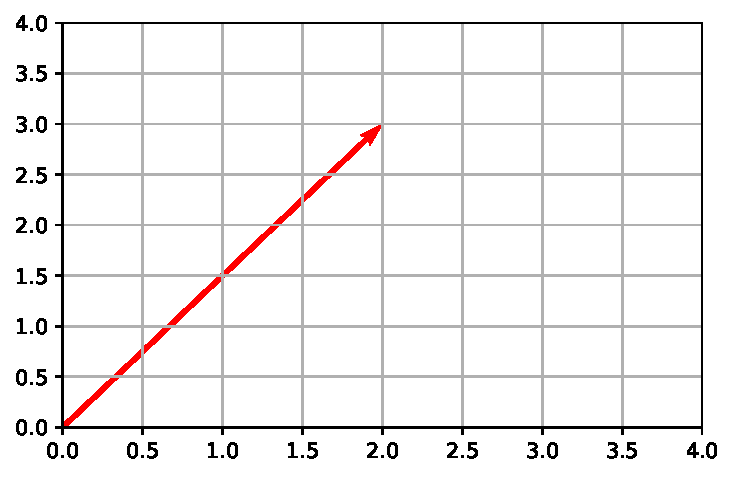
\includegraphics[keepaspectratio]{books/en-US/lab_files/figure-latex/cell-5-output-1.pdf}}

This makes a little arrow from the origin \texttt{(0,0)} to
\texttt{(2,3)}.

\subsubsection{Try It Yourself}\label{try-it-yourself-100}

\begin{enumerate}
\def\labelenumi{\arabic{enumi}.}
\tightlist
\item
  Change the vector \texttt{v} to \texttt{{[}4,\ 1{]}}. Where does the
  arrow point now?
\item
  Try making a 3D vector with 4 numbers, like
  \texttt{{[}1,\ 2,\ 3,\ 4{]}}. What happens?
\item
  Replace \texttt{np.array({[}2,3{]})} with
  \texttt{np.array({[}0,0{]})}. What does the arrow look like?
\end{enumerate}

\subsection{2. Vector Notation, Components, and
Arrows}\label{vector-notation-components-and-arrows-1}

In this lab, we'll practice reading, writing, and visualizing vectors in
different ways. A vector can look simple at first - just a list of
numbers - but how we \emph{write} it and how we \emph{interpret} it
really matters. This is where notation and components come into play.

A vector has:

\begin{itemize}
\tightlist
\item
  A symbol (we might call it \texttt{v}, \texttt{w}, or even
  \texttt{→AB} in geometry).
\item
  Components (the individual numbers, like \texttt{2} and \texttt{3} in
  \texttt{{[}2,\ 3{]}}).
\item
  An arrow picture (a geometric way to see the vector as a directed line
  segment).
\end{itemize}

Let's see all three in action with Python.

\subsubsection{Set Up Your Lab}\label{set-up-your-lab-1}

\begin{Shaded}
\begin{Highlighting}[]
\ImportTok{import}\NormalTok{ numpy }\ImportTok{as}\NormalTok{ np}
\ImportTok{import}\NormalTok{ matplotlib.pyplot }\ImportTok{as}\NormalTok{ plt}
\end{Highlighting}
\end{Shaded}

\subsubsection{Step-by-Step Code
Walkthrough}\label{step-by-step-code-walkthrough-1}

\begin{enumerate}
\def\labelenumi{\arabic{enumi}.}
\tightlist
\item
  Writing vectors in Python
\end{enumerate}

\begin{Shaded}
\begin{Highlighting}[]
\CommentTok{\# Two{-}dimensional vector}
\NormalTok{v }\OperatorTok{=}\NormalTok{ np.array([}\DecValTok{2}\NormalTok{, }\DecValTok{3}\NormalTok{])}

\CommentTok{\# Three{-}dimensional vector}
\NormalTok{w }\OperatorTok{=}\NormalTok{ np.array([}\DecValTok{1}\NormalTok{, }\OperatorTok{{-}}\DecValTok{1}\NormalTok{, }\DecValTok{4}\NormalTok{])}

\BuiltInTok{print}\NormalTok{(}\StringTok{"v ="}\NormalTok{, v)}
\BuiltInTok{print}\NormalTok{(}\StringTok{"w ="}\NormalTok{, w)}
\end{Highlighting}
\end{Shaded}

\begin{verbatim}
v = [2 3]
w = [ 1 -1  4]
\end{verbatim}

Here \texttt{v} has components \texttt{(2,\ 3)} and \texttt{w} has
components \texttt{(1,\ -1,\ 4)}.

\begin{enumerate}
\def\labelenumi{\arabic{enumi}.}
\setcounter{enumi}{1}
\tightlist
\item
  Accessing components Each number in the vector is a \emph{component}.
  We can pick them out using indexing.
\end{enumerate}

\begin{Shaded}
\begin{Highlighting}[]
\BuiltInTok{print}\NormalTok{(}\StringTok{"First component of v:"}\NormalTok{, v[}\DecValTok{0}\NormalTok{])}
\BuiltInTok{print}\NormalTok{(}\StringTok{"Second component of v:"}\NormalTok{, v[}\DecValTok{1}\NormalTok{])}
\end{Highlighting}
\end{Shaded}

\begin{verbatim}
First component of v: 2
Second component of v: 3
\end{verbatim}

Notice: in Python, indices start at \texttt{0}, so \texttt{v{[}0{]}} is
the \emph{first} component.

\begin{enumerate}
\def\labelenumi{\arabic{enumi}.}
\setcounter{enumi}{2}
\tightlist
\item
  Visualizing vectors as arrows In 2D, it's easy to draw a vector from
  the origin \texttt{(0,0)} to its endpoint \texttt{(x,y)}.
\end{enumerate}

\begin{Shaded}
\begin{Highlighting}[]
\NormalTok{plt.quiver(}\DecValTok{0}\NormalTok{, }\DecValTok{0}\NormalTok{, v[}\DecValTok{0}\NormalTok{], v[}\DecValTok{1}\NormalTok{], angles}\OperatorTok{=}\StringTok{\textquotesingle{}xy\textquotesingle{}}\NormalTok{, scale\_units}\OperatorTok{=}\StringTok{\textquotesingle{}xy\textquotesingle{}}\NormalTok{, scale}\OperatorTok{=}\DecValTok{1}\NormalTok{, color}\OperatorTok{=}\StringTok{\textquotesingle{}r\textquotesingle{}}\NormalTok{)}
\NormalTok{plt.xlim(}\OperatorTok{{-}}\DecValTok{1}\NormalTok{, }\DecValTok{4}\NormalTok{)}
\NormalTok{plt.ylim(}\OperatorTok{{-}}\DecValTok{2}\NormalTok{, }\DecValTok{4}\NormalTok{)}
\NormalTok{plt.axhline(}\DecValTok{0}\NormalTok{, color}\OperatorTok{=}\StringTok{\textquotesingle{}black\textquotesingle{}}\NormalTok{, linewidth}\OperatorTok{=}\FloatTok{0.5}\NormalTok{)}
\NormalTok{plt.axvline(}\DecValTok{0}\NormalTok{, color}\OperatorTok{=}\StringTok{\textquotesingle{}black\textquotesingle{}}\NormalTok{, linewidth}\OperatorTok{=}\FloatTok{0.5}\NormalTok{)}
\NormalTok{plt.grid()}
\NormalTok{plt.show()}
\end{Highlighting}
\end{Shaded}

\pandocbounded{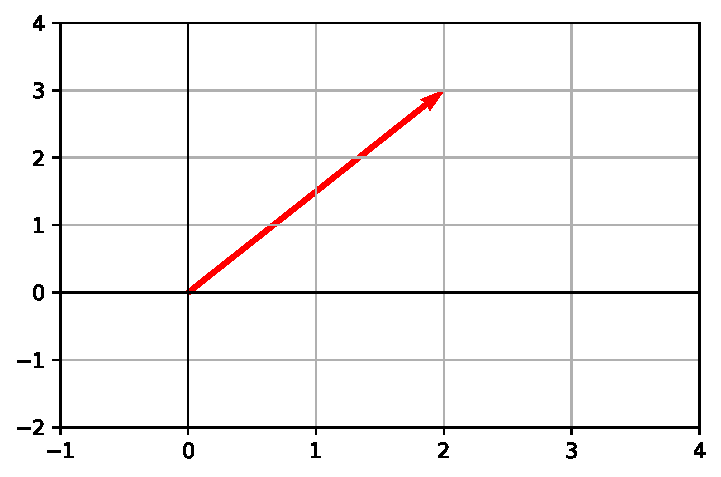
\includegraphics[keepaspectratio]{books/en-US/lab_files/figure-latex/cell-9-output-1.pdf}}

This shows vector v as a red arrow from \texttt{(0,0)} to
\texttt{(2,3)}.

\begin{enumerate}
\def\labelenumi{\arabic{enumi}.}
\setcounter{enumi}{3}
\tightlist
\item
  Drawing multiple vectors We can plot several arrows at once to compare
  them.
\end{enumerate}

\begin{Shaded}
\begin{Highlighting}[]
\NormalTok{u }\OperatorTok{=}\NormalTok{ np.array([}\DecValTok{3}\NormalTok{, }\DecValTok{1}\NormalTok{])}
\NormalTok{z }\OperatorTok{=}\NormalTok{ np.array([}\OperatorTok{{-}}\DecValTok{1}\NormalTok{, }\DecValTok{2}\NormalTok{])}

\CommentTok{\# Draw v, u, z in different colors}
\NormalTok{plt.quiver(}\DecValTok{0}\NormalTok{, }\DecValTok{0}\NormalTok{, v[}\DecValTok{0}\NormalTok{], v[}\DecValTok{1}\NormalTok{], angles}\OperatorTok{=}\StringTok{\textquotesingle{}xy\textquotesingle{}}\NormalTok{, scale\_units}\OperatorTok{=}\StringTok{\textquotesingle{}xy\textquotesingle{}}\NormalTok{, scale}\OperatorTok{=}\DecValTok{1}\NormalTok{, color}\OperatorTok{=}\StringTok{\textquotesingle{}r\textquotesingle{}}\NormalTok{, label}\OperatorTok{=}\StringTok{\textquotesingle{}v\textquotesingle{}}\NormalTok{)}
\NormalTok{plt.quiver(}\DecValTok{0}\NormalTok{, }\DecValTok{0}\NormalTok{, u[}\DecValTok{0}\NormalTok{], u[}\DecValTok{1}\NormalTok{], angles}\OperatorTok{=}\StringTok{\textquotesingle{}xy\textquotesingle{}}\NormalTok{, scale\_units}\OperatorTok{=}\StringTok{\textquotesingle{}xy\textquotesingle{}}\NormalTok{, scale}\OperatorTok{=}\DecValTok{1}\NormalTok{, color}\OperatorTok{=}\StringTok{\textquotesingle{}b\textquotesingle{}}\NormalTok{, label}\OperatorTok{=}\StringTok{\textquotesingle{}u\textquotesingle{}}\NormalTok{)}
\NormalTok{plt.quiver(}\DecValTok{0}\NormalTok{, }\DecValTok{0}\NormalTok{, z[}\DecValTok{0}\NormalTok{], z[}\DecValTok{1}\NormalTok{], angles}\OperatorTok{=}\StringTok{\textquotesingle{}xy\textquotesingle{}}\NormalTok{, scale\_units}\OperatorTok{=}\StringTok{\textquotesingle{}xy\textquotesingle{}}\NormalTok{, scale}\OperatorTok{=}\DecValTok{1}\NormalTok{, color}\OperatorTok{=}\StringTok{\textquotesingle{}g\textquotesingle{}}\NormalTok{, label}\OperatorTok{=}\StringTok{\textquotesingle{}z\textquotesingle{}}\NormalTok{)}

\NormalTok{plt.xlim(}\OperatorTok{{-}}\DecValTok{2}\NormalTok{, }\DecValTok{4}\NormalTok{)}
\NormalTok{plt.ylim(}\OperatorTok{{-}}\DecValTok{2}\NormalTok{, }\DecValTok{4}\NormalTok{)}
\NormalTok{plt.axhline(}\DecValTok{0}\NormalTok{, color}\OperatorTok{=}\StringTok{\textquotesingle{}black\textquotesingle{}}\NormalTok{, linewidth}\OperatorTok{=}\FloatTok{0.5}\NormalTok{)}
\NormalTok{plt.axvline(}\DecValTok{0}\NormalTok{, color}\OperatorTok{=}\StringTok{\textquotesingle{}black\textquotesingle{}}\NormalTok{, linewidth}\OperatorTok{=}\FloatTok{0.5}\NormalTok{)}
\NormalTok{plt.grid()}
\NormalTok{plt.show()}
\end{Highlighting}
\end{Shaded}

\pandocbounded{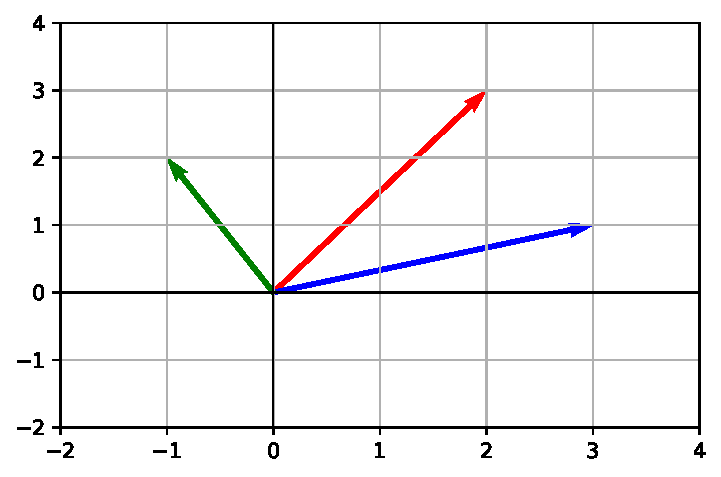
\includegraphics[keepaspectratio]{books/en-US/lab_files/figure-latex/cell-10-output-1.pdf}}

Now you'll see three arrows starting at the same point, each pointing in
a different direction.

\subsubsection{Try It Yourself}\label{try-it-yourself-101}

\begin{enumerate}
\def\labelenumi{\arabic{enumi}.}
\tightlist
\item
  Change \texttt{v} to \texttt{{[}5,\ 0{]}}. What does the arrow look
  like now?
\item
  Try a vector like \texttt{{[}0,\ -3{]}}. Which axis does it line up
  with?
\item
  Make a new vector \texttt{q\ =\ np.array({[}2,\ 0,\ 0{]})}. What
  happens if you try to plot it with \texttt{plt.quiver} in 2D?
\end{enumerate}

\subsection{3. Vector Addition and Scalar
Multiplication}\label{vector-addition-and-scalar-multiplication-1}

In this lab, we'll explore the two most fundamental operations you can
perform with vectors: adding them together and scaling them by a number
(a scalar). These operations form the basis of everything else in linear
algebra, from geometry to machine learning. Understanding how they work,
both in code and visually, is key to building intuition.

\subsubsection{Set Up Your Lab}\label{set-up-your-lab-2}

\begin{Shaded}
\begin{Highlighting}[]
\ImportTok{import}\NormalTok{ numpy }\ImportTok{as}\NormalTok{ np}
\ImportTok{import}\NormalTok{ matplotlib.pyplot }\ImportTok{as}\NormalTok{ plt}
\end{Highlighting}
\end{Shaded}

\subsubsection{Step-by-Step Code
Walkthrough}\label{step-by-step-code-walkthrough-2}

\begin{enumerate}
\def\labelenumi{\arabic{enumi}.}
\tightlist
\item
  Vector addition When you add two vectors, you simply add their
  components one by one.
\end{enumerate}

\begin{Shaded}
\begin{Highlighting}[]
\NormalTok{v }\OperatorTok{=}\NormalTok{ np.array([}\DecValTok{2}\NormalTok{, }\DecValTok{3}\NormalTok{])}
\NormalTok{u }\OperatorTok{=}\NormalTok{ np.array([}\DecValTok{1}\NormalTok{, }\OperatorTok{{-}}\DecValTok{1}\NormalTok{])}

\NormalTok{sum\_vector }\OperatorTok{=}\NormalTok{ v }\OperatorTok{+}\NormalTok{ u}
\BuiltInTok{print}\NormalTok{(}\StringTok{"v + u ="}\NormalTok{, sum\_vector)}
\end{Highlighting}
\end{Shaded}

\begin{verbatim}
v + u = [3 2]
\end{verbatim}

Here, \texttt{(2,3)\ +\ (1,-1)\ =\ (3,2)}.

\begin{enumerate}
\def\labelenumi{\arabic{enumi}.}
\setcounter{enumi}{1}
\tightlist
\item
  Visualizing vector addition (tip-to-tail method) Graphically, vector
  addition means placing the tail of one vector at the head of the
  other. The resulting vector goes from the start of the first to the
  end of the second.
\end{enumerate}

\begin{Shaded}
\begin{Highlighting}[]
\NormalTok{plt.quiver(}\DecValTok{0}\NormalTok{, }\DecValTok{0}\NormalTok{, v[}\DecValTok{0}\NormalTok{], v[}\DecValTok{1}\NormalTok{], angles}\OperatorTok{=}\StringTok{\textquotesingle{}xy\textquotesingle{}}\NormalTok{, scale\_units}\OperatorTok{=}\StringTok{\textquotesingle{}xy\textquotesingle{}}\NormalTok{, scale}\OperatorTok{=}\DecValTok{1}\NormalTok{, color}\OperatorTok{=}\StringTok{\textquotesingle{}r\textquotesingle{}}\NormalTok{, label}\OperatorTok{=}\StringTok{\textquotesingle{}v\textquotesingle{}}\NormalTok{)}
\NormalTok{plt.quiver(v[}\DecValTok{0}\NormalTok{], v[}\DecValTok{1}\NormalTok{], u[}\DecValTok{0}\NormalTok{], u[}\DecValTok{1}\NormalTok{], angles}\OperatorTok{=}\StringTok{\textquotesingle{}xy\textquotesingle{}}\NormalTok{, scale\_units}\OperatorTok{=}\StringTok{\textquotesingle{}xy\textquotesingle{}}\NormalTok{, scale}\OperatorTok{=}\DecValTok{1}\NormalTok{, color}\OperatorTok{=}\StringTok{\textquotesingle{}b\textquotesingle{}}\NormalTok{, label}\OperatorTok{=}\StringTok{\textquotesingle{}u placed at end of v\textquotesingle{}}\NormalTok{)}
\NormalTok{plt.quiver(}\DecValTok{0}\NormalTok{, }\DecValTok{0}\NormalTok{, sum\_vector[}\DecValTok{0}\NormalTok{], sum\_vector[}\DecValTok{1}\NormalTok{], angles}\OperatorTok{=}\StringTok{\textquotesingle{}xy\textquotesingle{}}\NormalTok{, scale\_units}\OperatorTok{=}\StringTok{\textquotesingle{}xy\textquotesingle{}}\NormalTok{, scale}\OperatorTok{=}\DecValTok{1}\NormalTok{, color}\OperatorTok{=}\StringTok{\textquotesingle{}g\textquotesingle{}}\NormalTok{, label}\OperatorTok{=}\StringTok{\textquotesingle{}v + u\textquotesingle{}}\NormalTok{)}

\NormalTok{plt.xlim(}\OperatorTok{{-}}\DecValTok{1}\NormalTok{, }\DecValTok{5}\NormalTok{)}
\NormalTok{plt.ylim(}\OperatorTok{{-}}\DecValTok{2}\NormalTok{, }\DecValTok{5}\NormalTok{)}
\NormalTok{plt.axhline(}\DecValTok{0}\NormalTok{, color}\OperatorTok{=}\StringTok{\textquotesingle{}black\textquotesingle{}}\NormalTok{, linewidth}\OperatorTok{=}\FloatTok{0.5}\NormalTok{)}
\NormalTok{plt.axvline(}\DecValTok{0}\NormalTok{, color}\OperatorTok{=}\StringTok{\textquotesingle{}black\textquotesingle{}}\NormalTok{, linewidth}\OperatorTok{=}\FloatTok{0.5}\NormalTok{)}
\NormalTok{plt.grid()}
\NormalTok{plt.show()}
\end{Highlighting}
\end{Shaded}

\pandocbounded{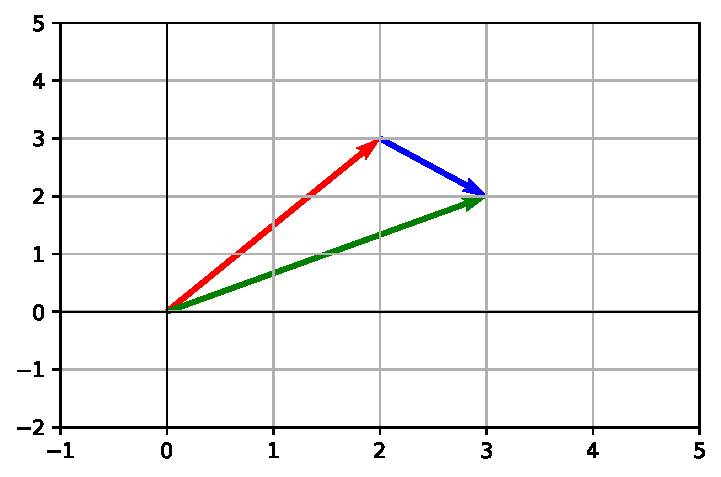
\includegraphics[keepaspectratio]{books/en-US/lab_files/figure-latex/cell-13-output-1.pdf}}

The green arrow is the result of adding \texttt{v} and \texttt{u}.

\begin{enumerate}
\def\labelenumi{\arabic{enumi}.}
\setcounter{enumi}{2}
\tightlist
\item
  Scalar multiplication Multiplying a vector by a scalar stretches or
  shrinks it. If the scalar is negative, the vector flips direction.
\end{enumerate}

\begin{Shaded}
\begin{Highlighting}[]
\NormalTok{c }\OperatorTok{=} \DecValTok{2}
\NormalTok{scaled\_v }\OperatorTok{=}\NormalTok{ c }\OperatorTok{*}\NormalTok{ v}
\BuiltInTok{print}\NormalTok{(}\StringTok{"2 * v ="}\NormalTok{, scaled\_v)}

\NormalTok{d }\OperatorTok{=} \OperatorTok{{-}}\DecValTok{1}
\NormalTok{scaled\_v\_neg }\OperatorTok{=}\NormalTok{ d }\OperatorTok{*}\NormalTok{ v}
\BuiltInTok{print}\NormalTok{(}\StringTok{"{-}1 * v ="}\NormalTok{, scaled\_v\_neg)}
\end{Highlighting}
\end{Shaded}

\begin{verbatim}
2 * v = [4 6]
-1 * v = [-2 -3]
\end{verbatim}

So \texttt{2\ *\ (2,3)\ =\ (4,6)} and \texttt{-1\ *\ (2,3)\ =\ (-2,-3)}.

\begin{enumerate}
\def\labelenumi{\arabic{enumi}.}
\setcounter{enumi}{3}
\tightlist
\item
  Visualizing scalar multiplication
\end{enumerate}

\begin{Shaded}
\begin{Highlighting}[]
\NormalTok{plt.quiver(}\DecValTok{0}\NormalTok{, }\DecValTok{0}\NormalTok{, v[}\DecValTok{0}\NormalTok{], v[}\DecValTok{1}\NormalTok{], angles}\OperatorTok{=}\StringTok{\textquotesingle{}xy\textquotesingle{}}\NormalTok{, scale\_units}\OperatorTok{=}\StringTok{\textquotesingle{}xy\textquotesingle{}}\NormalTok{, scale}\OperatorTok{=}\DecValTok{1}\NormalTok{, color}\OperatorTok{=}\StringTok{\textquotesingle{}r\textquotesingle{}}\NormalTok{, label}\OperatorTok{=}\StringTok{\textquotesingle{}v\textquotesingle{}}\NormalTok{)}
\NormalTok{plt.quiver(}\DecValTok{0}\NormalTok{, }\DecValTok{0}\NormalTok{, scaled\_v[}\DecValTok{0}\NormalTok{], scaled\_v[}\DecValTok{1}\NormalTok{], angles}\OperatorTok{=}\StringTok{\textquotesingle{}xy\textquotesingle{}}\NormalTok{, scale\_units}\OperatorTok{=}\StringTok{\textquotesingle{}xy\textquotesingle{}}\NormalTok{, scale}\OperatorTok{=}\DecValTok{1}\NormalTok{, color}\OperatorTok{=}\StringTok{\textquotesingle{}b\textquotesingle{}}\NormalTok{, label}\OperatorTok{=}\StringTok{\textquotesingle{}2 * v\textquotesingle{}}\NormalTok{)}
\NormalTok{plt.quiver(}\DecValTok{0}\NormalTok{, }\DecValTok{0}\NormalTok{, scaled\_v\_neg[}\DecValTok{0}\NormalTok{], scaled\_v\_neg[}\DecValTok{1}\NormalTok{], angles}\OperatorTok{=}\StringTok{\textquotesingle{}xy\textquotesingle{}}\NormalTok{, scale\_units}\OperatorTok{=}\StringTok{\textquotesingle{}xy\textquotesingle{}}\NormalTok{, scale}\OperatorTok{=}\DecValTok{1}\NormalTok{, color}\OperatorTok{=}\StringTok{\textquotesingle{}g\textquotesingle{}}\NormalTok{, label}\OperatorTok{=}\StringTok{\textquotesingle{}{-}1 * v\textquotesingle{}}\NormalTok{)}

\NormalTok{plt.xlim(}\OperatorTok{{-}}\DecValTok{5}\NormalTok{, }\DecValTok{5}\NormalTok{)}
\NormalTok{plt.ylim(}\OperatorTok{{-}}\DecValTok{5}\NormalTok{, }\DecValTok{7}\NormalTok{)}
\NormalTok{plt.axhline(}\DecValTok{0}\NormalTok{, color}\OperatorTok{=}\StringTok{\textquotesingle{}black\textquotesingle{}}\NormalTok{, linewidth}\OperatorTok{=}\FloatTok{0.5}\NormalTok{)}
\NormalTok{plt.axvline(}\DecValTok{0}\NormalTok{, color}\OperatorTok{=}\StringTok{\textquotesingle{}black\textquotesingle{}}\NormalTok{, linewidth}\OperatorTok{=}\FloatTok{0.5}\NormalTok{)}
\NormalTok{plt.grid()}
\NormalTok{plt.show()}
\end{Highlighting}
\end{Shaded}

\pandocbounded{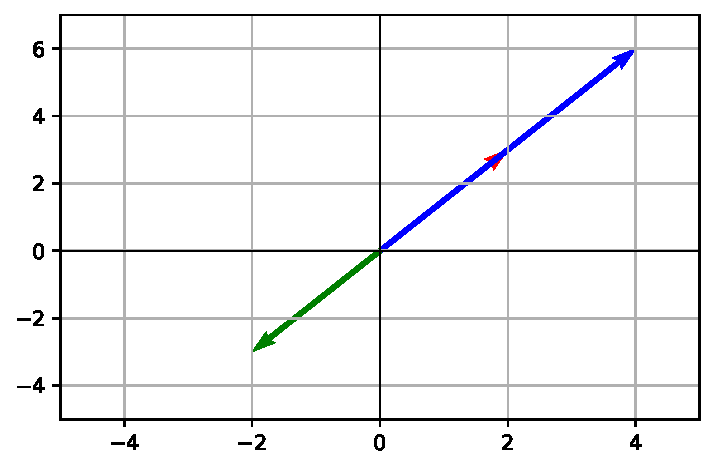
\includegraphics[keepaspectratio]{books/en-US/lab_files/figure-latex/cell-15-output-1.pdf}}

Here, the blue arrow is twice as long as the red arrow, while the green
arrow points in the opposite direction.

\begin{enumerate}
\def\labelenumi{\arabic{enumi}.}
\setcounter{enumi}{4}
\tightlist
\item
  Combining both operations We can scale vectors and then add them. This
  is called a linear combination (and it's the foundation for the next
  section).
\end{enumerate}

\begin{Shaded}
\begin{Highlighting}[]
\NormalTok{combo }\OperatorTok{=} \DecValTok{3}\OperatorTok{*}\NormalTok{v }\OperatorTok{+}\NormalTok{ (}\OperatorTok{{-}}\DecValTok{2}\NormalTok{)}\OperatorTok{*}\NormalTok{u}
\BuiltInTok{print}\NormalTok{(}\StringTok{"3*v {-} 2*u ="}\NormalTok{, combo)}
\end{Highlighting}
\end{Shaded}

\begin{verbatim}
3*v - 2*u = [ 4 11]
\end{verbatim}

\subsubsection{Try It Yourself}\label{try-it-yourself-102}

\begin{enumerate}
\def\labelenumi{\arabic{enumi}.}
\tightlist
\item
  Replace \texttt{c\ =\ 2} with \texttt{c\ =\ 0.5}. What happens to the
  vector?
\item
  Try adding three vectors: \texttt{v\ +\ u\ +\ np.array({[}-1,2{]})}.
  Can you predict the result before printing?
\item
  Visualize \texttt{3*v\ +\ 2*u} using arrows. How does it compare to
  just \texttt{v\ +\ u}?
\end{enumerate}

\subsection{4. Linear Combinations and
Span}\label{linear-combinations-and-span-1}

Now that we know how to add vectors and scale them, we can combine these
two moves to create linear combinations. A linear combination is just a
recipe: multiply vectors by scalars, then add them together. The set of
all possible results you can get from such recipes is called the span.

This idea is powerful because span tells us what directions and regions
of space we can reach using given vectors.

\subsubsection{Set Up Your Lab}\label{set-up-your-lab-3}

\begin{Shaded}
\begin{Highlighting}[]
\ImportTok{import}\NormalTok{ numpy }\ImportTok{as}\NormalTok{ np}
\ImportTok{import}\NormalTok{ matplotlib.pyplot }\ImportTok{as}\NormalTok{ plt}
\end{Highlighting}
\end{Shaded}

\subsubsection{Step-by-Step Code
Walkthrough}\label{step-by-step-code-walkthrough-3}

\begin{enumerate}
\def\labelenumi{\arabic{enumi}.}
\tightlist
\item
  Linear combinations in Python
\end{enumerate}

\begin{Shaded}
\begin{Highlighting}[]
\NormalTok{v }\OperatorTok{=}\NormalTok{ np.array([}\DecValTok{2}\NormalTok{, }\DecValTok{1}\NormalTok{])}
\NormalTok{u }\OperatorTok{=}\NormalTok{ np.array([}\DecValTok{1}\NormalTok{, }\DecValTok{3}\NormalTok{])}

\NormalTok{combo1 }\OperatorTok{=} \DecValTok{2}\OperatorTok{*}\NormalTok{v }\OperatorTok{+} \DecValTok{3}\OperatorTok{*}\NormalTok{u}
\NormalTok{combo2 }\OperatorTok{=} \OperatorTok{{-}}\DecValTok{1}\OperatorTok{*}\NormalTok{v }\OperatorTok{+} \DecValTok{4}\OperatorTok{*}\NormalTok{u}

\BuiltInTok{print}\NormalTok{(}\StringTok{"2*v + 3*u ="}\NormalTok{, combo1)}
\BuiltInTok{print}\NormalTok{(}\StringTok{"{-}v + 4*u ="}\NormalTok{, combo2)}
\end{Highlighting}
\end{Shaded}

\begin{verbatim}
2*v + 3*u = [ 7 11]
-v + 4*u = [ 2 11]
\end{verbatim}

Here, we multiplied and added vectors using scalars. Each result is a
new vector.

\begin{enumerate}
\def\labelenumi{\arabic{enumi}.}
\setcounter{enumi}{1}
\tightlist
\item
  Visualizing linear combinations Let's plot \texttt{v}, \texttt{u}, and
  their combinations.
\end{enumerate}

\begin{Shaded}
\begin{Highlighting}[]
\NormalTok{plt.quiver(}\DecValTok{0}\NormalTok{, }\DecValTok{0}\NormalTok{, v[}\DecValTok{0}\NormalTok{], v[}\DecValTok{1}\NormalTok{], angles}\OperatorTok{=}\StringTok{\textquotesingle{}xy\textquotesingle{}}\NormalTok{, scale\_units}\OperatorTok{=}\StringTok{\textquotesingle{}xy\textquotesingle{}}\NormalTok{, scale}\OperatorTok{=}\DecValTok{1}\NormalTok{, color}\OperatorTok{=}\StringTok{\textquotesingle{}r\textquotesingle{}}\NormalTok{, label}\OperatorTok{=}\StringTok{\textquotesingle{}v\textquotesingle{}}\NormalTok{)}
\NormalTok{plt.quiver(}\DecValTok{0}\NormalTok{, }\DecValTok{0}\NormalTok{, u[}\DecValTok{0}\NormalTok{], u[}\DecValTok{1}\NormalTok{], angles}\OperatorTok{=}\StringTok{\textquotesingle{}xy\textquotesingle{}}\NormalTok{, scale\_units}\OperatorTok{=}\StringTok{\textquotesingle{}xy\textquotesingle{}}\NormalTok{, scale}\OperatorTok{=}\DecValTok{1}\NormalTok{, color}\OperatorTok{=}\StringTok{\textquotesingle{}b\textquotesingle{}}\NormalTok{, label}\OperatorTok{=}\StringTok{\textquotesingle{}u\textquotesingle{}}\NormalTok{)}
\NormalTok{plt.quiver(}\DecValTok{0}\NormalTok{, }\DecValTok{0}\NormalTok{, combo1[}\DecValTok{0}\NormalTok{], combo1[}\DecValTok{1}\NormalTok{], angles}\OperatorTok{=}\StringTok{\textquotesingle{}xy\textquotesingle{}}\NormalTok{, scale\_units}\OperatorTok{=}\StringTok{\textquotesingle{}xy\textquotesingle{}}\NormalTok{, scale}\OperatorTok{=}\DecValTok{1}\NormalTok{, color}\OperatorTok{=}\StringTok{\textquotesingle{}g\textquotesingle{}}\NormalTok{, label}\OperatorTok{=}\StringTok{\textquotesingle{}2v + 3u\textquotesingle{}}\NormalTok{)}
\NormalTok{plt.quiver(}\DecValTok{0}\NormalTok{, }\DecValTok{0}\NormalTok{, combo2[}\DecValTok{0}\NormalTok{], combo2[}\DecValTok{1}\NormalTok{], angles}\OperatorTok{=}\StringTok{\textquotesingle{}xy\textquotesingle{}}\NormalTok{, scale\_units}\OperatorTok{=}\StringTok{\textquotesingle{}xy\textquotesingle{}}\NormalTok{, scale}\OperatorTok{=}\DecValTok{1}\NormalTok{, color}\OperatorTok{=}\StringTok{\textquotesingle{}m\textquotesingle{}}\NormalTok{, label}\OperatorTok{=}\StringTok{\textquotesingle{}{-}v + 4u\textquotesingle{}}\NormalTok{)}

\NormalTok{plt.xlim(}\OperatorTok{{-}}\DecValTok{5}\NormalTok{, }\DecValTok{10}\NormalTok{)}
\NormalTok{plt.ylim(}\OperatorTok{{-}}\DecValTok{5}\NormalTok{, }\DecValTok{10}\NormalTok{)}
\NormalTok{plt.axhline(}\DecValTok{0}\NormalTok{, color}\OperatorTok{=}\StringTok{\textquotesingle{}black\textquotesingle{}}\NormalTok{, linewidth}\OperatorTok{=}\FloatTok{0.5}\NormalTok{)}
\NormalTok{plt.axvline(}\DecValTok{0}\NormalTok{, color}\OperatorTok{=}\StringTok{\textquotesingle{}black\textquotesingle{}}\NormalTok{, linewidth}\OperatorTok{=}\FloatTok{0.5}\NormalTok{)}
\NormalTok{plt.grid()}
\NormalTok{plt.show()}
\end{Highlighting}
\end{Shaded}

\pandocbounded{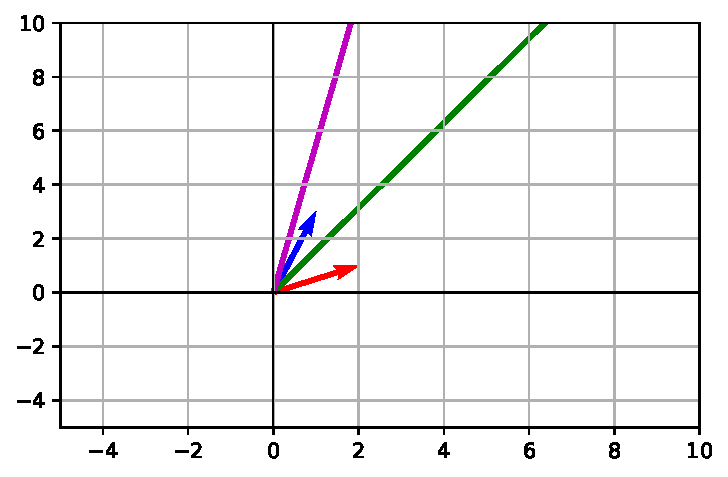
\includegraphics[keepaspectratio]{books/en-US/lab_files/figure-latex/cell-19-output-1.pdf}}

This shows how new arrows can be generated from scaling and adding the
original ones.

\begin{enumerate}
\def\labelenumi{\arabic{enumi}.}
\setcounter{enumi}{2}
\tightlist
\item
  Exploring the span The span of two 2D vectors is either:
\end{enumerate}

\begin{itemize}
\tightlist
\item
  A line (if one is a multiple of the other).
\item
  The whole 2D plane (if they are independent).
\end{itemize}

\begin{Shaded}
\begin{Highlighting}[]
\CommentTok{\# Generate many combinations}
\NormalTok{coeffs }\OperatorTok{=} \BuiltInTok{range}\NormalTok{(}\OperatorTok{{-}}\DecValTok{5}\NormalTok{, }\DecValTok{6}\NormalTok{)}
\NormalTok{points }\OperatorTok{=}\NormalTok{ []}
\ControlFlowTok{for}\NormalTok{ a }\KeywordTok{in}\NormalTok{ coeffs:}
    \ControlFlowTok{for}\NormalTok{ b }\KeywordTok{in}\NormalTok{ coeffs:}
\NormalTok{        point }\OperatorTok{=}\NormalTok{ a}\OperatorTok{*}\NormalTok{v }\OperatorTok{+}\NormalTok{ b}\OperatorTok{*}\NormalTok{u}
\NormalTok{        points.append(point)}

\NormalTok{points }\OperatorTok{=}\NormalTok{ np.array(points)}

\NormalTok{plt.scatter(points[:,}\DecValTok{0}\NormalTok{], points[:,}\DecValTok{1}\NormalTok{], s}\OperatorTok{=}\DecValTok{10}\NormalTok{, color}\OperatorTok{=}\StringTok{\textquotesingle{}gray\textquotesingle{}}\NormalTok{)}
\NormalTok{plt.quiver(}\DecValTok{0}\NormalTok{, }\DecValTok{0}\NormalTok{, v[}\DecValTok{0}\NormalTok{], v[}\DecValTok{1}\NormalTok{], angles}\OperatorTok{=}\StringTok{\textquotesingle{}xy\textquotesingle{}}\NormalTok{, scale\_units}\OperatorTok{=}\StringTok{\textquotesingle{}xy\textquotesingle{}}\NormalTok{, scale}\OperatorTok{=}\DecValTok{1}\NormalTok{, color}\OperatorTok{=}\StringTok{\textquotesingle{}r\textquotesingle{}}\NormalTok{)}
\NormalTok{plt.quiver(}\DecValTok{0}\NormalTok{, }\DecValTok{0}\NormalTok{, u[}\DecValTok{0}\NormalTok{], u[}\DecValTok{1}\NormalTok{], angles}\OperatorTok{=}\StringTok{\textquotesingle{}xy\textquotesingle{}}\NormalTok{, scale\_units}\OperatorTok{=}\StringTok{\textquotesingle{}xy\textquotesingle{}}\NormalTok{, scale}\OperatorTok{=}\DecValTok{1}\NormalTok{, color}\OperatorTok{=}\StringTok{\textquotesingle{}b\textquotesingle{}}\NormalTok{)}

\NormalTok{plt.xlim(}\OperatorTok{{-}}\DecValTok{10}\NormalTok{, }\DecValTok{10}\NormalTok{)}
\NormalTok{plt.ylim(}\OperatorTok{{-}}\DecValTok{10}\NormalTok{, }\DecValTok{10}\NormalTok{)}
\NormalTok{plt.axhline(}\DecValTok{0}\NormalTok{, color}\OperatorTok{=}\StringTok{\textquotesingle{}black\textquotesingle{}}\NormalTok{, linewidth}\OperatorTok{=}\FloatTok{0.5}\NormalTok{)}
\NormalTok{plt.axvline(}\DecValTok{0}\NormalTok{, color}\OperatorTok{=}\StringTok{\textquotesingle{}black\textquotesingle{}}\NormalTok{, linewidth}\OperatorTok{=}\FloatTok{0.5}\NormalTok{)}
\NormalTok{plt.grid()}
\NormalTok{plt.show()}
\end{Highlighting}
\end{Shaded}

\pandocbounded{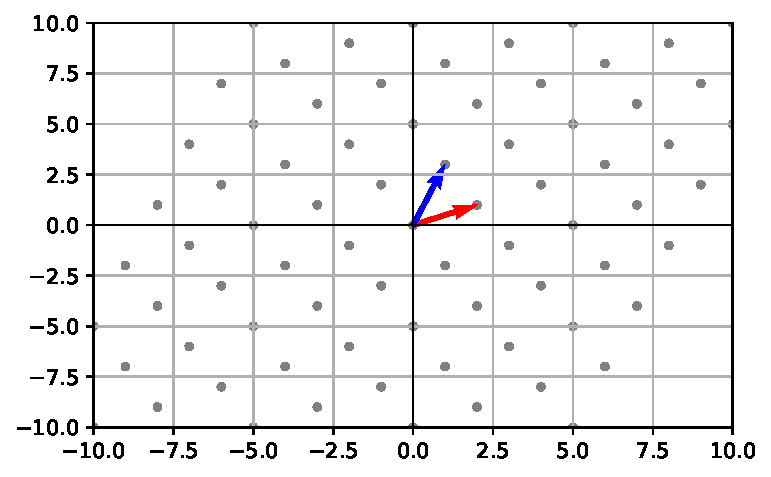
\includegraphics[keepaspectratio]{books/en-US/lab_files/figure-latex/cell-20-output-1.pdf}}

The gray dots show all reachable points with combinations of \texttt{v}
and \texttt{u}.

\begin{enumerate}
\def\labelenumi{\arabic{enumi}.}
\setcounter{enumi}{3}
\tightlist
\item
  Special case: dependent vectors
\end{enumerate}

\begin{Shaded}
\begin{Highlighting}[]
\NormalTok{w }\OperatorTok{=}\NormalTok{ np.array([}\DecValTok{4}\NormalTok{, }\DecValTok{2}\NormalTok{])  }\CommentTok{\# notice w = 2*v}
\NormalTok{coeffs }\OperatorTok{=} \BuiltInTok{range}\NormalTok{(}\OperatorTok{{-}}\DecValTok{5}\NormalTok{, }\DecValTok{6}\NormalTok{)}
\NormalTok{points }\OperatorTok{=}\NormalTok{ []}
\ControlFlowTok{for}\NormalTok{ a }\KeywordTok{in}\NormalTok{ coeffs:}
    \ControlFlowTok{for}\NormalTok{ b }\KeywordTok{in}\NormalTok{ coeffs:}
\NormalTok{        points.append(a}\OperatorTok{*}\NormalTok{v }\OperatorTok{+}\NormalTok{ b}\OperatorTok{*}\NormalTok{w)}

\NormalTok{points }\OperatorTok{=}\NormalTok{ np.array(points)}

\NormalTok{plt.scatter(points[:,}\DecValTok{0}\NormalTok{], points[:,}\DecValTok{1}\NormalTok{], s}\OperatorTok{=}\DecValTok{10}\NormalTok{, color}\OperatorTok{=}\StringTok{\textquotesingle{}gray\textquotesingle{}}\NormalTok{)}
\NormalTok{plt.quiver(}\DecValTok{0}\NormalTok{, }\DecValTok{0}\NormalTok{, v[}\DecValTok{0}\NormalTok{], v[}\DecValTok{1}\NormalTok{], angles}\OperatorTok{=}\StringTok{\textquotesingle{}xy\textquotesingle{}}\NormalTok{, scale\_units}\OperatorTok{=}\StringTok{\textquotesingle{}xy\textquotesingle{}}\NormalTok{, scale}\OperatorTok{=}\DecValTok{1}\NormalTok{, color}\OperatorTok{=}\StringTok{\textquotesingle{}r\textquotesingle{}}\NormalTok{)}
\NormalTok{plt.quiver(}\DecValTok{0}\NormalTok{, }\DecValTok{0}\NormalTok{, w[}\DecValTok{0}\NormalTok{], w[}\DecValTok{1}\NormalTok{], angles}\OperatorTok{=}\StringTok{\textquotesingle{}xy\textquotesingle{}}\NormalTok{, scale\_units}\OperatorTok{=}\StringTok{\textquotesingle{}xy\textquotesingle{}}\NormalTok{, scale}\OperatorTok{=}\DecValTok{1}\NormalTok{, color}\OperatorTok{=}\StringTok{\textquotesingle{}b\textquotesingle{}}\NormalTok{)}

\NormalTok{plt.xlim(}\OperatorTok{{-}}\DecValTok{10}\NormalTok{, }\DecValTok{10}\NormalTok{)}
\NormalTok{plt.ylim(}\OperatorTok{{-}}\DecValTok{10}\NormalTok{, }\DecValTok{10}\NormalTok{)}
\NormalTok{plt.axhline(}\DecValTok{0}\NormalTok{, color}\OperatorTok{=}\StringTok{\textquotesingle{}black\textquotesingle{}}\NormalTok{, linewidth}\OperatorTok{=}\FloatTok{0.5}\NormalTok{)}
\NormalTok{plt.axvline(}\DecValTok{0}\NormalTok{, color}\OperatorTok{=}\StringTok{\textquotesingle{}black\textquotesingle{}}\NormalTok{, linewidth}\OperatorTok{=}\FloatTok{0.5}\NormalTok{)}
\NormalTok{plt.grid()}
\NormalTok{plt.show()}
\end{Highlighting}
\end{Shaded}

\pandocbounded{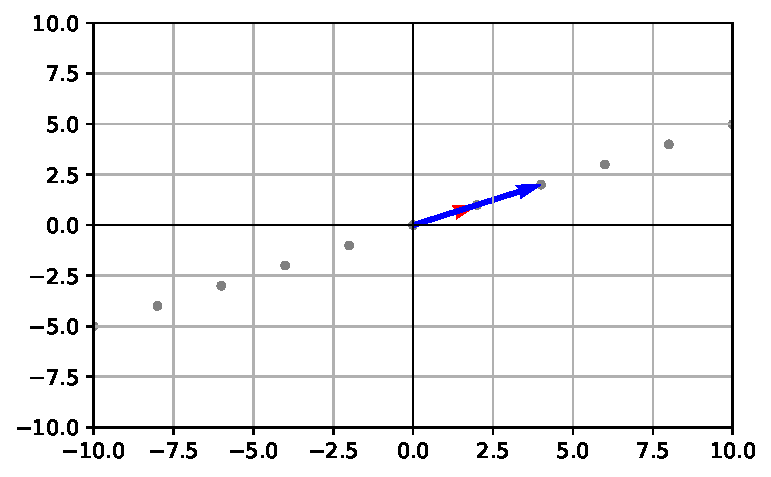
\includegraphics[keepaspectratio]{books/en-US/lab_files/figure-latex/cell-21-output-1.pdf}}

Here, the span collapses to a line because \texttt{w} is just a scaled
copy of \texttt{v}.

\subsubsection{Try It Yourself}\label{try-it-yourself-103}

\begin{enumerate}
\def\labelenumi{\arabic{enumi}.}
\tightlist
\item
  Replace \texttt{u\ =\ {[}1,3{]}} with \texttt{u\ =\ {[}-1,2{]}}. What
  does the span look like?
\item
  Try three vectors in 2D (e.g., \texttt{v,\ u,\ w}). Do you get more
  than the whole plane?
\item
  Experiment with 3D vectors. Use \texttt{np.array({[}x,y,z{]})} and
  check whether different vectors span a plane or all of space.
\end{enumerate}

\subsection{5. Length (Norm) and
Distance}\label{length-norm-and-distance-1}

In this lab, we'll measure how big a vector is (its length, also called
its norm) and how far apart two vectors are (their distance). These
ideas connect algebra to geometry: when we compute a norm, we're
measuring the size of an arrow; when we compute a distance, we're
measuring the gap between two points in space.

\subsubsection{Set Up Your Lab}\label{set-up-your-lab-4}

\begin{Shaded}
\begin{Highlighting}[]
\ImportTok{import}\NormalTok{ numpy }\ImportTok{as}\NormalTok{ np}
\ImportTok{import}\NormalTok{ matplotlib.pyplot }\ImportTok{as}\NormalTok{ plt}
\end{Highlighting}
\end{Shaded}

\subsubsection{Step-by-Step Code
Walkthrough}\label{step-by-step-code-walkthrough-4}

\begin{enumerate}
\def\labelenumi{\arabic{enumi}.}
\tightlist
\item
  Vector length (norm) in 2D The length of a vector is computed using
  the Pythagorean theorem. For a vector \texttt{(x,\ y)}, the length is
  \texttt{sqrt(x²\ +\ y²)}.
\end{enumerate}

\begin{Shaded}
\begin{Highlighting}[]
\NormalTok{v }\OperatorTok{=}\NormalTok{ np.array([}\DecValTok{3}\NormalTok{, }\DecValTok{4}\NormalTok{])}
\NormalTok{length }\OperatorTok{=}\NormalTok{ np.linalg.norm(v)}
\BuiltInTok{print}\NormalTok{(}\StringTok{"Length of v ="}\NormalTok{, length)}
\end{Highlighting}
\end{Shaded}

\begin{verbatim}
Length of v = 5.0
\end{verbatim}

This prints \texttt{5.0}, because \texttt{(3,4)} forms a right triangle
with sides 3 and 4, and \texttt{sqrt(3²+4²)=5}.

\begin{enumerate}
\def\labelenumi{\arabic{enumi}.}
\setcounter{enumi}{1}
\tightlist
\item
  Manual calculation vs NumPy
\end{enumerate}

\begin{Shaded}
\begin{Highlighting}[]
\NormalTok{manual\_length }\OperatorTok{=}\NormalTok{ (v[}\DecValTok{0}\NormalTok{]}\OperatorTok{**}\DecValTok{2} \OperatorTok{+}\NormalTok{ v[}\DecValTok{1}\NormalTok{]}\OperatorTok{**}\DecValTok{2}\NormalTok{)}\OperatorTok{**}\FloatTok{0.5}
\BuiltInTok{print}\NormalTok{(}\StringTok{"Manual length ="}\NormalTok{, manual\_length)}
\BuiltInTok{print}\NormalTok{(}\StringTok{"NumPy length ="}\NormalTok{, np.linalg.norm(v))}
\end{Highlighting}
\end{Shaded}

\begin{verbatim}
Manual length = 5.0
NumPy length = 5.0
\end{verbatim}

Both give the same result.

\begin{enumerate}
\def\labelenumi{\arabic{enumi}.}
\setcounter{enumi}{2}
\tightlist
\item
  Visualizing vector length
\end{enumerate}

\begin{Shaded}
\begin{Highlighting}[]
\NormalTok{plt.quiver(}\DecValTok{0}\NormalTok{, }\DecValTok{0}\NormalTok{, v[}\DecValTok{0}\NormalTok{], v[}\DecValTok{1}\NormalTok{], angles}\OperatorTok{=}\StringTok{\textquotesingle{}xy\textquotesingle{}}\NormalTok{, scale\_units}\OperatorTok{=}\StringTok{\textquotesingle{}xy\textquotesingle{}}\NormalTok{, scale}\OperatorTok{=}\DecValTok{1}\NormalTok{, color}\OperatorTok{=}\StringTok{\textquotesingle{}r\textquotesingle{}}\NormalTok{)}
\NormalTok{plt.xlim(}\DecValTok{0}\NormalTok{, }\DecValTok{5}\NormalTok{)}
\NormalTok{plt.ylim(}\DecValTok{0}\NormalTok{, }\DecValTok{5}\NormalTok{)}
\NormalTok{plt.axhline(}\DecValTok{0}\NormalTok{, color}\OperatorTok{=}\StringTok{\textquotesingle{}black\textquotesingle{}}\NormalTok{, linewidth}\OperatorTok{=}\FloatTok{0.5}\NormalTok{)}
\NormalTok{plt.axvline(}\DecValTok{0}\NormalTok{, color}\OperatorTok{=}\StringTok{\textquotesingle{}black\textquotesingle{}}\NormalTok{, linewidth}\OperatorTok{=}\FloatTok{0.5}\NormalTok{)}
\NormalTok{plt.text(v[}\DecValTok{0}\NormalTok{]}\OperatorTok{/}\DecValTok{2}\NormalTok{, v[}\DecValTok{1}\NormalTok{]}\OperatorTok{/}\DecValTok{2}\NormalTok{, }\SpecialStringTok{f"Length=}\SpecialCharTok{\{}\NormalTok{length}\SpecialCharTok{\}}\SpecialStringTok{"}\NormalTok{, fontsize}\OperatorTok{=}\DecValTok{10}\NormalTok{, color}\OperatorTok{=}\StringTok{\textquotesingle{}blue\textquotesingle{}}\NormalTok{)}
\NormalTok{plt.grid()}
\NormalTok{plt.show()}
\end{Highlighting}
\end{Shaded}

\pandocbounded{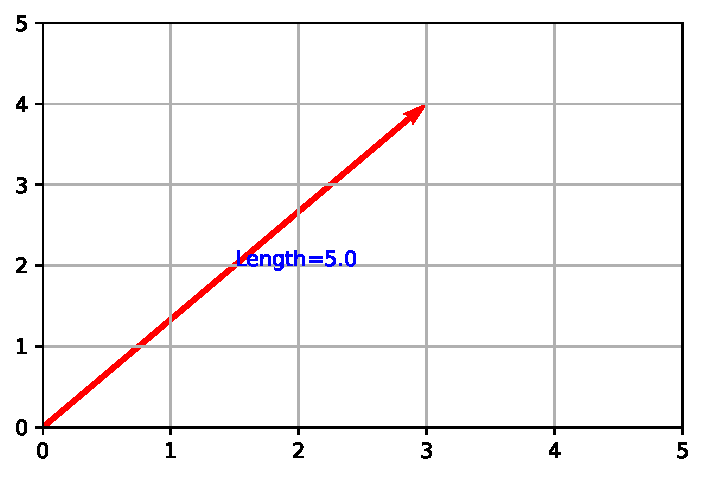
\includegraphics[keepaspectratio]{books/en-US/lab_files/figure-latex/cell-25-output-1.pdf}}

You'll see the arrow \texttt{(3,4)} with its length labeled.

\begin{enumerate}
\def\labelenumi{\arabic{enumi}.}
\setcounter{enumi}{3}
\tightlist
\item
  Distance between two vectors The distance between \texttt{v} and
  another vector \texttt{u} is the length of their difference:
  \texttt{‖v\ -\ u‖}.
\end{enumerate}

\begin{Shaded}
\begin{Highlighting}[]
\NormalTok{u }\OperatorTok{=}\NormalTok{ np.array([}\DecValTok{0}\NormalTok{, }\DecValTok{0}\NormalTok{])   }\CommentTok{\# the origin}
\NormalTok{dist }\OperatorTok{=}\NormalTok{ np.linalg.norm(v }\OperatorTok{{-}}\NormalTok{ u)}
\BuiltInTok{print}\NormalTok{(}\StringTok{"Distance between v and u ="}\NormalTok{, dist)}
\end{Highlighting}
\end{Shaded}

\begin{verbatim}
Distance between v and u = 5.0
\end{verbatim}

Since \texttt{u} is the origin, this is just the length of \texttt{v}.

\begin{enumerate}
\def\labelenumi{\arabic{enumi}.}
\setcounter{enumi}{4}
\tightlist
\item
  A more interesting distance
\end{enumerate}

\begin{Shaded}
\begin{Highlighting}[]
\NormalTok{u }\OperatorTok{=}\NormalTok{ np.array([}\DecValTok{1}\NormalTok{, }\DecValTok{1}\NormalTok{])}
\NormalTok{dist }\OperatorTok{=}\NormalTok{ np.linalg.norm(v }\OperatorTok{{-}}\NormalTok{ u)}
\BuiltInTok{print}\NormalTok{(}\StringTok{"Distance between v and u ="}\NormalTok{, dist)}
\end{Highlighting}
\end{Shaded}

\begin{verbatim}
Distance between v and u = 3.605551275463989
\end{verbatim}

This measures how far \texttt{(3,4)} is from \texttt{(1,1)}.

\begin{enumerate}
\def\labelenumi{\arabic{enumi}.}
\setcounter{enumi}{5}
\tightlist
\item
  Visualizing distance between points
\end{enumerate}

\begin{Shaded}
\begin{Highlighting}[]
\NormalTok{plt.scatter([v[}\DecValTok{0}\NormalTok{], u[}\DecValTok{0}\NormalTok{]], [v[}\DecValTok{1}\NormalTok{], u[}\DecValTok{1}\NormalTok{]], color}\OperatorTok{=}\NormalTok{[}\StringTok{\textquotesingle{}red\textquotesingle{}}\NormalTok{,}\StringTok{\textquotesingle{}blue\textquotesingle{}}\NormalTok{])}
\NormalTok{plt.plot([v[}\DecValTok{0}\NormalTok{], u[}\DecValTok{0}\NormalTok{]], [v[}\DecValTok{1}\NormalTok{], u[}\DecValTok{1}\NormalTok{]], }\StringTok{\textquotesingle{}k{-}{-}\textquotesingle{}}\NormalTok{)}
\NormalTok{plt.text(v[}\DecValTok{0}\NormalTok{], v[}\DecValTok{1}\NormalTok{], }\StringTok{\textquotesingle{}v\textquotesingle{}}\NormalTok{, fontsize}\OperatorTok{=}\DecValTok{12}\NormalTok{, color}\OperatorTok{=}\StringTok{\textquotesingle{}red\textquotesingle{}}\NormalTok{)}
\NormalTok{plt.text(u[}\DecValTok{0}\NormalTok{], u[}\DecValTok{1}\NormalTok{], }\StringTok{\textquotesingle{}u\textquotesingle{}}\NormalTok{, fontsize}\OperatorTok{=}\DecValTok{12}\NormalTok{, color}\OperatorTok{=}\StringTok{\textquotesingle{}blue\textquotesingle{}}\NormalTok{)}
\NormalTok{plt.grid()}
\NormalTok{plt.show()}
\end{Highlighting}
\end{Shaded}

\pandocbounded{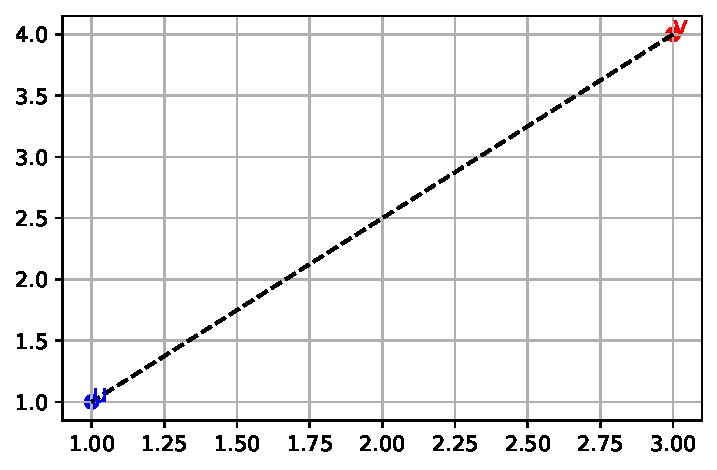
\includegraphics[keepaspectratio]{books/en-US/lab_files/figure-latex/cell-28-output-1.pdf}}

The dashed line shows the distance between the two points.

\begin{enumerate}
\def\labelenumi{\arabic{enumi}.}
\setcounter{enumi}{6}
\tightlist
\item
  Higher-dimensional vectors Norms and distances work the same way in
  any dimension:
\end{enumerate}

\begin{Shaded}
\begin{Highlighting}[]
\NormalTok{a }\OperatorTok{=}\NormalTok{ np.array([}\DecValTok{1}\NormalTok{,}\DecValTok{2}\NormalTok{,}\DecValTok{3}\NormalTok{])}
\NormalTok{b }\OperatorTok{=}\NormalTok{ np.array([}\DecValTok{4}\NormalTok{,}\DecValTok{0}\NormalTok{,}\DecValTok{8}\NormalTok{])}
\BuiltInTok{print}\NormalTok{(}\StringTok{"‖a‖ ="}\NormalTok{, np.linalg.norm(a))}
\BuiltInTok{print}\NormalTok{(}\StringTok{"‖b‖ ="}\NormalTok{, np.linalg.norm(b))}
\BuiltInTok{print}\NormalTok{(}\StringTok{"Distance between a and b ="}\NormalTok{, np.linalg.norm(a}\OperatorTok{{-}}\NormalTok{b))}
\end{Highlighting}
\end{Shaded}

\begin{verbatim}
‖a‖ = 3.7416573867739413
‖b‖ = 8.94427190999916
Distance between a and b = 6.164414002968976
\end{verbatim}

Even though we can't draw 3D easily on paper, the formulas still apply.

\subsubsection{Try It Yourself}\label{try-it-yourself-104}

\begin{enumerate}
\def\labelenumi{\arabic{enumi}.}
\tightlist
\item
  Compute the length of \texttt{np.array({[}5,12{]})}. What do you
  expect?
\item
  Find the distance between \texttt{(2,3)} and \texttt{(7,7)}. Can you
  sketch it by hand and check?
\item
  In 3D, try vectors \texttt{(1,1,1)} and \texttt{(2,2,2)}. Why is the
  distance exactly \texttt{sqrt(3)}?
\end{enumerate}

\subsection{6. Dot Product}\label{dot-product}

The dot product is one of the most important operations in linear
algebra. It takes two vectors and gives you a single number. That number
combines both the lengths of the vectors and how much they point in the
same direction. In this lab, we'll calculate dot products in several
ways, see how they relate to geometry, and visualize their meaning.

\subsubsection{Set Up Your Lab}\label{set-up-your-lab-5}

\begin{Shaded}
\begin{Highlighting}[]
\ImportTok{import}\NormalTok{ numpy }\ImportTok{as}\NormalTok{ np}
\ImportTok{import}\NormalTok{ matplotlib.pyplot }\ImportTok{as}\NormalTok{ plt}
\end{Highlighting}
\end{Shaded}

\subsubsection{Step-by-Step Code
Walkthrough}\label{step-by-step-code-walkthrough-5}

\begin{enumerate}
\def\labelenumi{\arabic{enumi}.}
\tightlist
\item
  Algebraic definition The dot product of two vectors is the sum of the
  products of their components:
\end{enumerate}

\begin{Shaded}
\begin{Highlighting}[]
\NormalTok{v }\OperatorTok{=}\NormalTok{ np.array([}\DecValTok{2}\NormalTok{, }\DecValTok{3}\NormalTok{])}
\NormalTok{u }\OperatorTok{=}\NormalTok{ np.array([}\DecValTok{4}\NormalTok{, }\OperatorTok{{-}}\DecValTok{1}\NormalTok{])}

\NormalTok{dot\_manual }\OperatorTok{=}\NormalTok{ v[}\DecValTok{0}\NormalTok{]}\OperatorTok{*}\NormalTok{u[}\DecValTok{0}\NormalTok{] }\OperatorTok{+}\NormalTok{ v[}\DecValTok{1}\NormalTok{]}\OperatorTok{*}\NormalTok{u[}\DecValTok{1}\NormalTok{]}
\NormalTok{dot\_numpy }\OperatorTok{=}\NormalTok{ np.dot(v, u)}

\BuiltInTok{print}\NormalTok{(}\StringTok{"Manual dot product:"}\NormalTok{, dot\_manual)}
\BuiltInTok{print}\NormalTok{(}\StringTok{"NumPy dot product:"}\NormalTok{, dot\_numpy)}
\end{Highlighting}
\end{Shaded}

\begin{verbatim}
Manual dot product: 5
NumPy dot product: 5
\end{verbatim}

Here, \texttt{(2*4)\ +\ (3*-1)\ =\ 8\ -\ 3\ =\ 5}.

\begin{enumerate}
\def\labelenumi{\arabic{enumi}.}
\setcounter{enumi}{1}
\tightlist
\item
  Geometric definition The dot product also equals the product of the
  lengths of the vectors times the cosine of the angle between them:
\end{enumerate}

\[
v \cdot u = \|v\| \|u\| \cos \theta
\]

We can compute the angle:

\begin{Shaded}
\begin{Highlighting}[]
\NormalTok{norm\_v }\OperatorTok{=}\NormalTok{ np.linalg.norm(v)}
\NormalTok{norm\_u }\OperatorTok{=}\NormalTok{ np.linalg.norm(u)}

\NormalTok{cos\_theta }\OperatorTok{=}\NormalTok{ np.dot(v, u) }\OperatorTok{/}\NormalTok{ (norm\_v }\OperatorTok{*}\NormalTok{ norm\_u)}
\NormalTok{theta }\OperatorTok{=}\NormalTok{ np.arccos(cos\_theta)}

\BuiltInTok{print}\NormalTok{(}\StringTok{"cos(theta) ="}\NormalTok{, cos\_theta)}
\BuiltInTok{print}\NormalTok{(}\StringTok{"theta (in radians) ="}\NormalTok{, theta)}
\BuiltInTok{print}\NormalTok{(}\StringTok{"theta (in degrees) ="}\NormalTok{, np.degrees(theta))}
\end{Highlighting}
\end{Shaded}

\begin{verbatim}
cos(theta) = 0.33633639699815626
theta (in radians) = 1.2277723863741932
theta (in degrees) = 70.3461759419467
\end{verbatim}

This gives the angle between \texttt{v} and \texttt{u}.

\begin{enumerate}
\def\labelenumi{\arabic{enumi}.}
\setcounter{enumi}{2}
\tightlist
\item
  Visualizing the dot product Let's draw the two vectors:
\end{enumerate}

\begin{Shaded}
\begin{Highlighting}[]
\NormalTok{plt.quiver(}\DecValTok{0}\NormalTok{,}\DecValTok{0}\NormalTok{,v[}\DecValTok{0}\NormalTok{],v[}\DecValTok{1}\NormalTok{],angles}\OperatorTok{=}\StringTok{\textquotesingle{}xy\textquotesingle{}}\NormalTok{,scale\_units}\OperatorTok{=}\StringTok{\textquotesingle{}xy\textquotesingle{}}\NormalTok{,scale}\OperatorTok{=}\DecValTok{1}\NormalTok{,color}\OperatorTok{=}\StringTok{\textquotesingle{}r\textquotesingle{}}\NormalTok{,label}\OperatorTok{=}\StringTok{\textquotesingle{}v\textquotesingle{}}\NormalTok{)}
\NormalTok{plt.quiver(}\DecValTok{0}\NormalTok{,}\DecValTok{0}\NormalTok{,u[}\DecValTok{0}\NormalTok{],u[}\DecValTok{1}\NormalTok{],angles}\OperatorTok{=}\StringTok{\textquotesingle{}xy\textquotesingle{}}\NormalTok{,scale\_units}\OperatorTok{=}\StringTok{\textquotesingle{}xy\textquotesingle{}}\NormalTok{,scale}\OperatorTok{=}\DecValTok{1}\NormalTok{,color}\OperatorTok{=}\StringTok{\textquotesingle{}b\textquotesingle{}}\NormalTok{,label}\OperatorTok{=}\StringTok{\textquotesingle{}u\textquotesingle{}}\NormalTok{)}
\NormalTok{plt.xlim(}\OperatorTok{{-}}\DecValTok{1}\NormalTok{,}\DecValTok{5}\NormalTok{)}
\NormalTok{plt.ylim(}\OperatorTok{{-}}\DecValTok{2}\NormalTok{,}\DecValTok{4}\NormalTok{)}
\NormalTok{plt.axhline(}\DecValTok{0}\NormalTok{,color}\OperatorTok{=}\StringTok{\textquotesingle{}black\textquotesingle{}}\NormalTok{,linewidth}\OperatorTok{=}\FloatTok{0.5}\NormalTok{)}
\NormalTok{plt.axvline(}\DecValTok{0}\NormalTok{,color}\OperatorTok{=}\StringTok{\textquotesingle{}black\textquotesingle{}}\NormalTok{,linewidth}\OperatorTok{=}\FloatTok{0.5}\NormalTok{)}
\NormalTok{plt.grid()}
\NormalTok{plt.show()}
\end{Highlighting}
\end{Shaded}

\pandocbounded{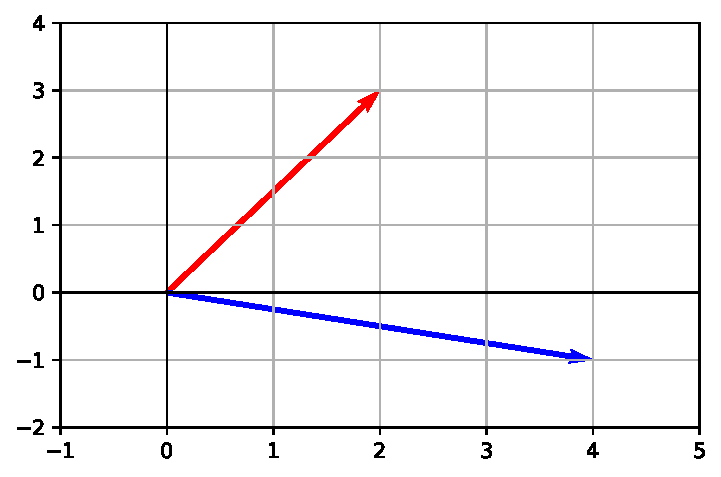
\includegraphics[keepaspectratio]{books/en-US/lab_files/figure-latex/cell-33-output-1.pdf}}

The dot product is positive if the angle is less than 90°, negative if
greater than 90°, and zero if the vectors are perpendicular.

\begin{enumerate}
\def\labelenumi{\arabic{enumi}.}
\setcounter{enumi}{3}
\tightlist
\item
  Projections and dot product The dot product lets us compute how much
  of one vector lies in the direction of another.
\end{enumerate}

\begin{Shaded}
\begin{Highlighting}[]
\NormalTok{proj\_length }\OperatorTok{=}\NormalTok{ np.dot(v, u) }\OperatorTok{/}\NormalTok{ np.linalg.norm(u)}
\BuiltInTok{print}\NormalTok{(}\StringTok{"Projection length of v onto u:"}\NormalTok{, proj\_length)}
\end{Highlighting}
\end{Shaded}

\begin{verbatim}
Projection length of v onto u: 1.212678125181665
\end{verbatim}

This is the length of the shadow of \texttt{v} onto \texttt{u}.

\begin{enumerate}
\def\labelenumi{\arabic{enumi}.}
\setcounter{enumi}{4}
\tightlist
\item
  Special cases
\end{enumerate}

\begin{itemize}
\tightlist
\item
  If vectors point in the same direction, the dot product is large and
  positive.
\item
  If vectors are perpendicular, the dot product is zero.
\item
  If vectors point in opposite directions, the dot product is negative.
\end{itemize}

\begin{Shaded}
\begin{Highlighting}[]
\NormalTok{a }\OperatorTok{=}\NormalTok{ np.array([}\DecValTok{1}\NormalTok{,}\DecValTok{0}\NormalTok{])}
\NormalTok{b }\OperatorTok{=}\NormalTok{ np.array([}\DecValTok{0}\NormalTok{,}\DecValTok{1}\NormalTok{])}
\NormalTok{c }\OperatorTok{=}\NormalTok{ np.array([}\OperatorTok{{-}}\DecValTok{1}\NormalTok{,}\DecValTok{0}\NormalTok{])}

\BuiltInTok{print}\NormalTok{(}\StringTok{"a · b ="}\NormalTok{, np.dot(a,b))   }\CommentTok{\# perpendicular}
\BuiltInTok{print}\NormalTok{(}\StringTok{"a · a ="}\NormalTok{, np.dot(a,a))   }\CommentTok{\# length squared}
\BuiltInTok{print}\NormalTok{(}\StringTok{"a · c ="}\NormalTok{, np.dot(a,c))   }\CommentTok{\# opposite}
\end{Highlighting}
\end{Shaded}

\begin{verbatim}
a · b = 0
a · a = 1
a · c = -1
\end{verbatim}

\subsubsection{Try It Yourself}\label{try-it-yourself-105}

\begin{enumerate}
\def\labelenumi{\arabic{enumi}.}
\tightlist
\item
  Compute the dot product of \texttt{(3,4)} with \texttt{(4,3)}. Is the
  result larger or smaller than the product of their lengths?
\item
  Try \texttt{(1,2,3)\ ·\ (4,5,6)}. Does the geometric meaning still
  work in 3D?
\item
  Create two perpendicular vectors (e.g.~\texttt{(2,0)} and
  \texttt{(0,5)}). Verify the dot product is zero.
\end{enumerate}

\subsection{7. Angles Between Vectors and
Cosine}\label{angles-between-vectors-and-cosine-1}

In this lab, we'll go deeper into the connection between vectors and
geometry by calculating angles. Angles tell us how much two vectors
``point in the same direction.'' The bridge between algebra and geometry
here is the cosine formula, which comes directly from the dot product.

\subsubsection{Set Up Your Lab}\label{set-up-your-lab-6}

\begin{Shaded}
\begin{Highlighting}[]
\ImportTok{import}\NormalTok{ numpy }\ImportTok{as}\NormalTok{ np}
\ImportTok{import}\NormalTok{ matplotlib.pyplot }\ImportTok{as}\NormalTok{ plt}
\end{Highlighting}
\end{Shaded}

\subsubsection{Step-by-Step Code
Walkthrough}\label{step-by-step-code-walkthrough-6}

\begin{enumerate}
\def\labelenumi{\arabic{enumi}.}
\tightlist
\item
  Formula for the angle The angle \(\theta\) between two vectors \(v\)
  and \(u\) is given by:
\end{enumerate}

\[
\cos \theta = \frac{v \cdot u}{\|v\| \, \|u\|}
\]

This means:

\begin{itemize}
\tightlist
\item
  If \(\cos \theta = 1\), the vectors point in exactly the same
  direction.
\item
  If \(\cos \theta = 0\), they are perpendicular.
\item
  If \(\cos \theta = -1\), they point in opposite directions.
\end{itemize}

\begin{enumerate}
\def\labelenumi{\arabic{enumi}.}
\setcounter{enumi}{1}
\tightlist
\item
  Computing the angle in Python
\end{enumerate}

\begin{Shaded}
\begin{Highlighting}[]
\NormalTok{v }\OperatorTok{=}\NormalTok{ np.array([}\DecValTok{2}\NormalTok{, }\DecValTok{3}\NormalTok{])}
\NormalTok{u }\OperatorTok{=}\NormalTok{ np.array([}\DecValTok{3}\NormalTok{, }\OperatorTok{{-}}\DecValTok{1}\NormalTok{])}

\NormalTok{dot }\OperatorTok{=}\NormalTok{ np.dot(v, u)}
\NormalTok{norm\_v }\OperatorTok{=}\NormalTok{ np.linalg.norm(v)}
\NormalTok{norm\_u }\OperatorTok{=}\NormalTok{ np.linalg.norm(u)}

\NormalTok{cos\_theta }\OperatorTok{=}\NormalTok{ dot }\OperatorTok{/}\NormalTok{ (norm\_v }\OperatorTok{*}\NormalTok{ norm\_u)}
\NormalTok{theta }\OperatorTok{=}\NormalTok{ np.arccos(cos\_theta)}

\BuiltInTok{print}\NormalTok{(}\StringTok{"cos(theta) ="}\NormalTok{, cos\_theta)}
\BuiltInTok{print}\NormalTok{(}\StringTok{"theta in radians ="}\NormalTok{, theta)}
\BuiltInTok{print}\NormalTok{(}\StringTok{"theta in degrees ="}\NormalTok{, np.degrees(theta))}
\end{Highlighting}
\end{Shaded}

\begin{verbatim}
cos(theta) = 0.2631174057921088
theta in radians = 1.3045442776439713
theta in degrees = 74.74488129694222
\end{verbatim}

This gives both the cosine value and the actual angle.

\begin{enumerate}
\def\labelenumi{\arabic{enumi}.}
\setcounter{enumi}{2}
\tightlist
\item
  Visualizing the vectors
\end{enumerate}

\begin{Shaded}
\begin{Highlighting}[]
\NormalTok{plt.quiver(}\DecValTok{0}\NormalTok{,}\DecValTok{0}\NormalTok{,v[}\DecValTok{0}\NormalTok{],v[}\DecValTok{1}\NormalTok{],angles}\OperatorTok{=}\StringTok{\textquotesingle{}xy\textquotesingle{}}\NormalTok{,scale\_units}\OperatorTok{=}\StringTok{\textquotesingle{}xy\textquotesingle{}}\NormalTok{,scale}\OperatorTok{=}\DecValTok{1}\NormalTok{,color}\OperatorTok{=}\StringTok{\textquotesingle{}r\textquotesingle{}}\NormalTok{,label}\OperatorTok{=}\StringTok{\textquotesingle{}v\textquotesingle{}}\NormalTok{)}
\NormalTok{plt.quiver(}\DecValTok{0}\NormalTok{,}\DecValTok{0}\NormalTok{,u[}\DecValTok{0}\NormalTok{],u[}\DecValTok{1}\NormalTok{],angles}\OperatorTok{=}\StringTok{\textquotesingle{}xy\textquotesingle{}}\NormalTok{,scale\_units}\OperatorTok{=}\StringTok{\textquotesingle{}xy\textquotesingle{}}\NormalTok{,scale}\OperatorTok{=}\DecValTok{1}\NormalTok{,color}\OperatorTok{=}\StringTok{\textquotesingle{}b\textquotesingle{}}\NormalTok{,label}\OperatorTok{=}\StringTok{\textquotesingle{}u\textquotesingle{}}\NormalTok{)}

\NormalTok{plt.xlim(}\OperatorTok{{-}}\DecValTok{1}\NormalTok{,}\DecValTok{4}\NormalTok{)}
\NormalTok{plt.ylim(}\OperatorTok{{-}}\DecValTok{2}\NormalTok{,}\DecValTok{4}\NormalTok{)}
\NormalTok{plt.axhline(}\DecValTok{0}\NormalTok{,color}\OperatorTok{=}\StringTok{\textquotesingle{}black\textquotesingle{}}\NormalTok{,linewidth}\OperatorTok{=}\FloatTok{0.5}\NormalTok{)}
\NormalTok{plt.axvline(}\DecValTok{0}\NormalTok{,color}\OperatorTok{=}\StringTok{\textquotesingle{}black\textquotesingle{}}\NormalTok{,linewidth}\OperatorTok{=}\FloatTok{0.5}\NormalTok{)}
\NormalTok{plt.grid()}
\NormalTok{plt.show()}
\end{Highlighting}
\end{Shaded}

\pandocbounded{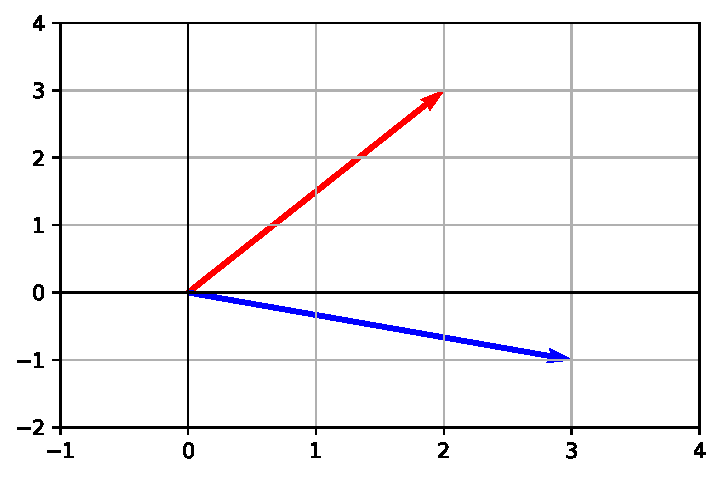
\includegraphics[keepaspectratio]{books/en-US/lab_files/figure-latex/cell-38-output-1.pdf}}

You can see the angle between \texttt{v} and \texttt{u} as the gap
between the red and blue arrows.

\begin{enumerate}
\def\labelenumi{\arabic{enumi}.}
\setcounter{enumi}{3}
\tightlist
\item
  Checking special cases
\end{enumerate}

\begin{Shaded}
\begin{Highlighting}[]
\NormalTok{a }\OperatorTok{=}\NormalTok{ np.array([}\DecValTok{1}\NormalTok{,}\DecValTok{0}\NormalTok{])}
\NormalTok{b }\OperatorTok{=}\NormalTok{ np.array([}\DecValTok{0}\NormalTok{,}\DecValTok{1}\NormalTok{])}
\NormalTok{c }\OperatorTok{=}\NormalTok{ np.array([}\OperatorTok{{-}}\DecValTok{1}\NormalTok{,}\DecValTok{0}\NormalTok{])}

\BuiltInTok{print}\NormalTok{(}\StringTok{"Angle between a and b ="}\NormalTok{, np.degrees(np.arccos(np.dot(a,b)}\OperatorTok{/}\NormalTok{(np.linalg.norm(a)}\OperatorTok{*}\NormalTok{np.linalg.norm(b)))))}
\BuiltInTok{print}\NormalTok{(}\StringTok{"Angle between a and c ="}\NormalTok{, np.degrees(np.arccos(np.dot(a,c)}\OperatorTok{/}\NormalTok{(np.linalg.norm(a)}\OperatorTok{*}\NormalTok{np.linalg.norm(c)))))}
\end{Highlighting}
\end{Shaded}

\begin{verbatim}
Angle between a and b = 90.0
Angle between a and c = 180.0
\end{verbatim}

\begin{itemize}
\tightlist
\item
  Angle between \texttt{(1,0)} and \texttt{(0,1)} is 90°.
\item
  Angle between \texttt{(1,0)} and \texttt{(-1,0)} is 180°.
\end{itemize}

\begin{enumerate}
\def\labelenumi{\arabic{enumi}.}
\setcounter{enumi}{4}
\tightlist
\item
  Using cosine as a similarity measure In data science and machine
  learning, people often use cosine similarity instead of raw angles.
  It's just the cosine value itself:
\end{enumerate}

\begin{Shaded}
\begin{Highlighting}[]
\NormalTok{cosine\_similarity }\OperatorTok{=}\NormalTok{ np.dot(v,u)}\OperatorTok{/}\NormalTok{(np.linalg.norm(v)}\OperatorTok{*}\NormalTok{np.linalg.norm(u))}
\BuiltInTok{print}\NormalTok{(}\StringTok{"Cosine similarity ="}\NormalTok{, cosine\_similarity)}
\end{Highlighting}
\end{Shaded}

\begin{verbatim}
Cosine similarity = 0.2631174057921088
\end{verbatim}

Values close to \texttt{1} mean vectors are aligned, values near
\texttt{0} mean unrelated, and values near \texttt{-1} mean opposite.

\subsubsection{Try It Yourself}\label{try-it-yourself-106}

\begin{enumerate}
\def\labelenumi{\arabic{enumi}.}
\tightlist
\item
  Create two random vectors with \texttt{np.random.randn(3)} and compute
  the angle between them.
\item
  Verify that swapping the vectors gives the same angle (symmetry).
\item
  Find two vectors where cosine similarity is exactly \texttt{0}. Can
  you come up with an example in 2D?
\end{enumerate}

\subsection{8. Projections and
Decompositions}\label{projections-and-decompositions-1}

In this lab, we'll learn how to split one vector into parts: one part
that lies \emph{along} another vector, and one part that is
\emph{perpendicular}. This process is called projection and
decomposition. Projections let us measure ``how much of a vector points
in a given direction,'' and decompositions give us a way to break
vectors into useful components.

\subsubsection{Set Up Your Lab}\label{set-up-your-lab-7}

\begin{Shaded}
\begin{Highlighting}[]
\ImportTok{import}\NormalTok{ numpy }\ImportTok{as}\NormalTok{ np}
\ImportTok{import}\NormalTok{ matplotlib.pyplot }\ImportTok{as}\NormalTok{ plt}
\end{Highlighting}
\end{Shaded}

\subsubsection{Step-by-Step Code
Walkthrough}\label{step-by-step-code-walkthrough-7}

\begin{enumerate}
\def\labelenumi{\arabic{enumi}.}
\tightlist
\item
  Projection formula The projection of vector \(v\) onto vector \(u\)
  is:
\end{enumerate}

\[
\text{proj}_u(v) = \frac{v \cdot u}{u \cdot u} \, u
\]

This gives the component of \(v\) that points in the direction of \(u\).

\begin{enumerate}
\def\labelenumi{\arabic{enumi}.}
\setcounter{enumi}{1}
\tightlist
\item
  Computing projection in Python
\end{enumerate}

\begin{Shaded}
\begin{Highlighting}[]
\NormalTok{v }\OperatorTok{=}\NormalTok{ np.array([}\DecValTok{3}\NormalTok{, }\DecValTok{2}\NormalTok{])}
\NormalTok{u }\OperatorTok{=}\NormalTok{ np.array([}\DecValTok{2}\NormalTok{, }\DecValTok{0}\NormalTok{])}

\NormalTok{proj\_u\_v }\OperatorTok{=}\NormalTok{ (np.dot(v, u) }\OperatorTok{/}\NormalTok{ np.dot(u, u)) }\OperatorTok{*}\NormalTok{ u}
\BuiltInTok{print}\NormalTok{(}\StringTok{"Projection of v onto u:"}\NormalTok{, proj\_u\_v)}
\end{Highlighting}
\end{Shaded}

\begin{verbatim}
Projection of v onto u: [3. 0.]
\end{verbatim}

Here, \(v = (3,2)\) and \(u = (2,0)\). The projection of \texttt{v} onto
\texttt{u} is a vector pointing along the x-axis.

\begin{enumerate}
\def\labelenumi{\arabic{enumi}.}
\setcounter{enumi}{2}
\tightlist
\item
  Decomposing into parallel and perpendicular parts
\end{enumerate}

We can write:

\[
v = \text{proj}_u(v) + (v - \text{proj}_u(v))
\]

The first part is parallel to \texttt{u}, the second part is
perpendicular.

\begin{Shaded}
\begin{Highlighting}[]
\NormalTok{perp }\OperatorTok{=}\NormalTok{ v }\OperatorTok{{-}}\NormalTok{ proj\_u\_v}
\BuiltInTok{print}\NormalTok{(}\StringTok{"Parallel part:"}\NormalTok{, proj\_u\_v)}
\BuiltInTok{print}\NormalTok{(}\StringTok{"Perpendicular part:"}\NormalTok{, perp)}
\end{Highlighting}
\end{Shaded}

\begin{verbatim}
Parallel part: [3. 0.]
Perpendicular part: [0. 2.]
\end{verbatim}

\begin{enumerate}
\def\labelenumi{\arabic{enumi}.}
\setcounter{enumi}{3}
\tightlist
\item
  Visualizing projection and decomposition
\end{enumerate}

\begin{Shaded}
\begin{Highlighting}[]
\NormalTok{plt.quiver(}\DecValTok{0}\NormalTok{, }\DecValTok{0}\NormalTok{, v[}\DecValTok{0}\NormalTok{], v[}\DecValTok{1}\NormalTok{], angles}\OperatorTok{=}\StringTok{\textquotesingle{}xy\textquotesingle{}}\NormalTok{, scale\_units}\OperatorTok{=}\StringTok{\textquotesingle{}xy\textquotesingle{}}\NormalTok{, scale}\OperatorTok{=}\DecValTok{1}\NormalTok{, color}\OperatorTok{=}\StringTok{\textquotesingle{}r\textquotesingle{}}\NormalTok{, label}\OperatorTok{=}\StringTok{\textquotesingle{}v\textquotesingle{}}\NormalTok{)}
\NormalTok{plt.quiver(}\DecValTok{0}\NormalTok{, }\DecValTok{0}\NormalTok{, u[}\DecValTok{0}\NormalTok{], u[}\DecValTok{1}\NormalTok{], angles}\OperatorTok{=}\StringTok{\textquotesingle{}xy\textquotesingle{}}\NormalTok{, scale\_units}\OperatorTok{=}\StringTok{\textquotesingle{}xy\textquotesingle{}}\NormalTok{, scale}\OperatorTok{=}\DecValTok{1}\NormalTok{, color}\OperatorTok{=}\StringTok{\textquotesingle{}b\textquotesingle{}}\NormalTok{, label}\OperatorTok{=}\StringTok{\textquotesingle{}u\textquotesingle{}}\NormalTok{)}
\NormalTok{plt.quiver(}\DecValTok{0}\NormalTok{, }\DecValTok{0}\NormalTok{, proj\_u\_v[}\DecValTok{0}\NormalTok{], proj\_u\_v[}\DecValTok{1}\NormalTok{], angles}\OperatorTok{=}\StringTok{\textquotesingle{}xy\textquotesingle{}}\NormalTok{, scale\_units}\OperatorTok{=}\StringTok{\textquotesingle{}xy\textquotesingle{}}\NormalTok{, scale}\OperatorTok{=}\DecValTok{1}\NormalTok{, color}\OperatorTok{=}\StringTok{\textquotesingle{}g\textquotesingle{}}\NormalTok{, label}\OperatorTok{=}\StringTok{\textquotesingle{}proj\_u(v)\textquotesingle{}}\NormalTok{)}
\NormalTok{plt.quiver(proj\_u\_v[}\DecValTok{0}\NormalTok{], proj\_u\_v[}\DecValTok{1}\NormalTok{], perp[}\DecValTok{0}\NormalTok{], perp[}\DecValTok{1}\NormalTok{], angles}\OperatorTok{=}\StringTok{\textquotesingle{}xy\textquotesingle{}}\NormalTok{, scale\_units}\OperatorTok{=}\StringTok{\textquotesingle{}xy\textquotesingle{}}\NormalTok{, scale}\OperatorTok{=}\DecValTok{1}\NormalTok{, color}\OperatorTok{=}\StringTok{\textquotesingle{}m\textquotesingle{}}\NormalTok{, label}\OperatorTok{=}\StringTok{\textquotesingle{}perpendicular\textquotesingle{}}\NormalTok{)}

\NormalTok{plt.xlim(}\OperatorTok{{-}}\DecValTok{1}\NormalTok{, }\DecValTok{5}\NormalTok{)}
\NormalTok{plt.ylim(}\OperatorTok{{-}}\DecValTok{1}\NormalTok{, }\DecValTok{4}\NormalTok{)}
\NormalTok{plt.axhline(}\DecValTok{0}\NormalTok{, color}\OperatorTok{=}\StringTok{\textquotesingle{}black\textquotesingle{}}\NormalTok{, linewidth}\OperatorTok{=}\FloatTok{0.5}\NormalTok{)}
\NormalTok{plt.axvline(}\DecValTok{0}\NormalTok{, color}\OperatorTok{=}\StringTok{\textquotesingle{}black\textquotesingle{}}\NormalTok{, linewidth}\OperatorTok{=}\FloatTok{0.5}\NormalTok{)}
\NormalTok{plt.grid()}
\NormalTok{plt.show()}
\end{Highlighting}
\end{Shaded}

\pandocbounded{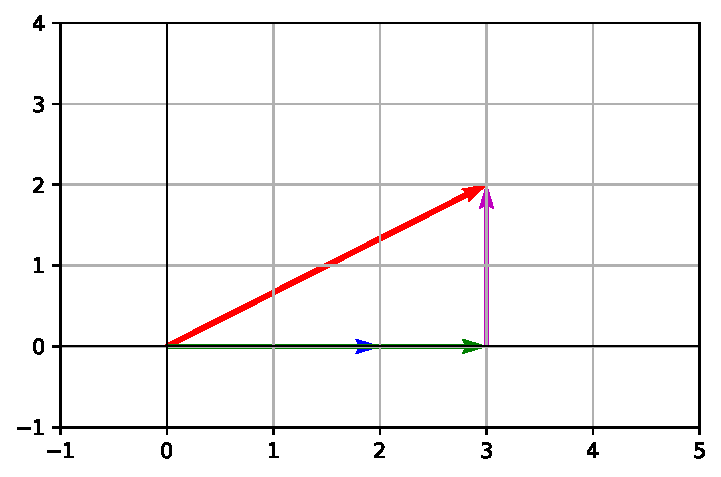
\includegraphics[keepaspectratio]{books/en-US/lab_files/figure-latex/cell-44-output-1.pdf}}

You'll see \texttt{v} (red), \texttt{u} (blue), the projection (green),
and the perpendicular remainder (magenta).

\begin{enumerate}
\def\labelenumi{\arabic{enumi}.}
\setcounter{enumi}{4}
\tightlist
\item
  Projection in higher dimensions
\end{enumerate}

This formula works in any dimension:

\begin{Shaded}
\begin{Highlighting}[]
\NormalTok{a }\OperatorTok{=}\NormalTok{ np.array([}\DecValTok{1}\NormalTok{,}\DecValTok{2}\NormalTok{,}\DecValTok{3}\NormalTok{])}
\NormalTok{b }\OperatorTok{=}\NormalTok{ np.array([}\DecValTok{0}\NormalTok{,}\DecValTok{1}\NormalTok{,}\DecValTok{0}\NormalTok{])}

\NormalTok{proj }\OperatorTok{=}\NormalTok{ (np.dot(a,b)}\OperatorTok{/}\NormalTok{np.dot(b,b)) }\OperatorTok{*}\NormalTok{ b}
\NormalTok{perp }\OperatorTok{=}\NormalTok{ a }\OperatorTok{{-}}\NormalTok{ proj}

\BuiltInTok{print}\NormalTok{(}\StringTok{"Projection of a onto b:"}\NormalTok{, proj)}
\BuiltInTok{print}\NormalTok{(}\StringTok{"Perpendicular component:"}\NormalTok{, perp)}
\end{Highlighting}
\end{Shaded}

\begin{verbatim}
Projection of a onto b: [0. 2. 0.]
Perpendicular component: [1. 0. 3.]
\end{verbatim}

Even in 3D or higher, projections are about splitting into ``along'' and
``across.''

\subsubsection{Try It Yourself}\label{try-it-yourself-107}

\begin{enumerate}
\def\labelenumi{\arabic{enumi}.}
\tightlist
\item
  Try projecting \texttt{(2,3)} onto \texttt{(0,5)}. Where does it land?
\item
  Take a 3D vector like \texttt{(4,2,6)} and project it onto
  \texttt{(1,0,0)}. What does this give you?
\item
  Change the base vector \texttt{u} to something not aligned with the
  axes, like \texttt{(1,1)}. Does the projection still work?
\end{enumerate}

\subsection{9. Cauchy--Schwarz and Triangle
Inequalities}\label{cauchyschwarz-and-triangle-inequalities-1}

This lab introduces two fundamental inequalities in linear algebra. They
may look abstract at first, but they provide guarantees that always hold
true for vectors. We'll explore them with small examples in Python to
see why they matter.

\subsubsection{Set Up Your Lab}\label{set-up-your-lab-8}

\begin{Shaded}
\begin{Highlighting}[]
\ImportTok{import}\NormalTok{ numpy }\ImportTok{as}\NormalTok{ np}
\end{Highlighting}
\end{Shaded}

\subsubsection{Step-by-Step Code
Walkthrough}\label{step-by-step-code-walkthrough-8}

\begin{enumerate}
\def\labelenumi{\arabic{enumi}.}
\tightlist
\item
  Cauchy--Schwarz inequality
\end{enumerate}

The inequality states:

\[
|v \cdot u| \leq \|v\| \, \|u\|
\]

It means the dot product is never ``bigger'' than the product of the
vector lengths. Equality happens only if the two vectors are pointing in
exactly the same (or opposite) direction.

\begin{Shaded}
\begin{Highlighting}[]
\NormalTok{v }\OperatorTok{=}\NormalTok{ np.array([}\DecValTok{3}\NormalTok{, }\DecValTok{4}\NormalTok{])}
\NormalTok{u }\OperatorTok{=}\NormalTok{ np.array([}\DecValTok{1}\NormalTok{, }\DecValTok{2}\NormalTok{])}

\NormalTok{lhs }\OperatorTok{=} \BuiltInTok{abs}\NormalTok{(np.dot(v, u))}
\NormalTok{rhs }\OperatorTok{=}\NormalTok{ np.linalg.norm(v) }\OperatorTok{*}\NormalTok{ np.linalg.norm(u)}

\BuiltInTok{print}\NormalTok{(}\StringTok{"Left{-}hand side (|v·u|):"}\NormalTok{, lhs)}
\BuiltInTok{print}\NormalTok{(}\StringTok{"Right{-}hand side (‖v‖‖u‖):"}\NormalTok{, rhs)}
\BuiltInTok{print}\NormalTok{(}\StringTok{"Inequality holds?"}\NormalTok{, lhs }\OperatorTok{\textless{}=}\NormalTok{ rhs)}
\end{Highlighting}
\end{Shaded}

\begin{verbatim}
Left-hand side (|v·u|): 11
Right-hand side (‖v‖‖u‖): 11.180339887498949
Inequality holds? True
\end{verbatim}

\begin{enumerate}
\def\labelenumi{\arabic{enumi}.}
\setcounter{enumi}{1}
\tightlist
\item
  Testing Cauchy--Schwarz with different vectors
\end{enumerate}

\begin{Shaded}
\begin{Highlighting}[]
\NormalTok{pairs }\OperatorTok{=}\NormalTok{ [}
\NormalTok{    (np.array([}\DecValTok{1}\NormalTok{,}\DecValTok{0}\NormalTok{]), np.array([}\DecValTok{0}\NormalTok{,}\DecValTok{1}\NormalTok{])),  }\CommentTok{\# perpendicular}
\NormalTok{    (np.array([}\DecValTok{2}\NormalTok{,}\DecValTok{3}\NormalTok{]), np.array([}\DecValTok{4}\NormalTok{,}\DecValTok{6}\NormalTok{])),  }\CommentTok{\# multiples}
\NormalTok{    (np.array([}\OperatorTok{{-}}\DecValTok{1}\NormalTok{,}\DecValTok{2}\NormalTok{]), np.array([}\DecValTok{3}\NormalTok{,}\OperatorTok{{-}}\DecValTok{6}\NormalTok{])) }\CommentTok{\# opposite multiples}
\NormalTok{]}

\ControlFlowTok{for}\NormalTok{ v,u }\KeywordTok{in}\NormalTok{ pairs:}
\NormalTok{    lhs }\OperatorTok{=} \BuiltInTok{abs}\NormalTok{(np.dot(v, u))}
\NormalTok{    rhs }\OperatorTok{=}\NormalTok{ np.linalg.norm(v) }\OperatorTok{*}\NormalTok{ np.linalg.norm(u)}
    \BuiltInTok{print}\NormalTok{(}\SpecialStringTok{f"v=}\SpecialCharTok{\{}\NormalTok{v}\SpecialCharTok{\}}\SpecialStringTok{, u=}\SpecialCharTok{\{}\NormalTok{u}\SpecialCharTok{\}}\SpecialStringTok{ {-}\textgreater{} |v·u|=}\SpecialCharTok{\{}\NormalTok{lhs}\SpecialCharTok{\}}\SpecialStringTok{, ‖v‖‖u‖=}\SpecialCharTok{\{}\NormalTok{rhs}\SpecialCharTok{\}}\SpecialStringTok{, holds=}\SpecialCharTok{\{}\NormalTok{lhs}\OperatorTok{\textless{}=}\NormalTok{rhs}\SpecialCharTok{\}}\SpecialStringTok{"}\NormalTok{)}
\end{Highlighting}
\end{Shaded}

\begin{verbatim}
v=[1 0], u=[0 1] -> |v·u|=0, ‖v‖‖u‖=1.0, holds=True
v=[2 3], u=[4 6] -> |v·u|=26, ‖v‖‖u‖=25.999999999999996, holds=False
v=[-1  2], u=[ 3 -6] -> |v·u|=15, ‖v‖‖u‖=15.000000000000002, holds=True
\end{verbatim}

\begin{itemize}
\tightlist
\item
  Perpendicular vectors give \texttt{\textbar{}v·u\textbar{}\ =\ 0}, far
  less than the product of norms.
\item
  Multiples give equality (\texttt{lhs\ =\ rhs}).
\end{itemize}

\begin{enumerate}
\def\labelenumi{\arabic{enumi}.}
\setcounter{enumi}{2}
\tightlist
\item
  Triangle inequality
\end{enumerate}

The triangle inequality states:

\[
\|v + u\| \leq \|v\| + \|u\|
\]

Geometrically, the length of one side of a triangle can never be longer
than the sum of the other two sides.

\begin{Shaded}
\begin{Highlighting}[]
\NormalTok{v }\OperatorTok{=}\NormalTok{ np.array([}\DecValTok{3}\NormalTok{, }\DecValTok{4}\NormalTok{])}
\NormalTok{u }\OperatorTok{=}\NormalTok{ np.array([}\DecValTok{1}\NormalTok{, }\DecValTok{2}\NormalTok{])}

\NormalTok{lhs }\OperatorTok{=}\NormalTok{ np.linalg.norm(v }\OperatorTok{+}\NormalTok{ u)}
\NormalTok{rhs }\OperatorTok{=}\NormalTok{ np.linalg.norm(v) }\OperatorTok{+}\NormalTok{ np.linalg.norm(u)}

\BuiltInTok{print}\NormalTok{(}\StringTok{"‖v+u‖ ="}\NormalTok{, lhs)}
\BuiltInTok{print}\NormalTok{(}\StringTok{"‖v‖ + ‖u‖ ="}\NormalTok{, rhs)}
\BuiltInTok{print}\NormalTok{(}\StringTok{"Inequality holds?"}\NormalTok{, lhs }\OperatorTok{\textless{}=}\NormalTok{ rhs)}
\end{Highlighting}
\end{Shaded}

\begin{verbatim}
‖v+u‖ = 7.211102550927978
‖v‖ + ‖u‖ = 7.23606797749979
Inequality holds? True
\end{verbatim}

\begin{enumerate}
\def\labelenumi{\arabic{enumi}.}
\setcounter{enumi}{3}
\tightlist
\item
  Visual demonstration with a triangle
\end{enumerate}

\begin{Shaded}
\begin{Highlighting}[]
\ImportTok{import}\NormalTok{ matplotlib.pyplot }\ImportTok{as}\NormalTok{ plt}

\NormalTok{origin }\OperatorTok{=}\NormalTok{ np.array([}\DecValTok{0}\NormalTok{,}\DecValTok{0}\NormalTok{])}
\NormalTok{points }\OperatorTok{=}\NormalTok{ np.array([origin, v, v}\OperatorTok{+}\NormalTok{u, origin])}

\NormalTok{plt.plot(points[:,}\DecValTok{0}\NormalTok{], points[:,}\DecValTok{1}\NormalTok{], }\StringTok{\textquotesingle{}ro{-}\textquotesingle{}}\NormalTok{)  }\CommentTok{\# triangle outline}
\NormalTok{plt.text(v[}\DecValTok{0}\NormalTok{], v[}\DecValTok{1}\NormalTok{], }\StringTok{\textquotesingle{}v\textquotesingle{}}\NormalTok{)}
\NormalTok{plt.text(v[}\DecValTok{0}\NormalTok{]}\OperatorTok{+}\NormalTok{u[}\DecValTok{0}\NormalTok{], v[}\DecValTok{1}\NormalTok{]}\OperatorTok{+}\NormalTok{u[}\DecValTok{1}\NormalTok{], }\StringTok{\textquotesingle{}v+u\textquotesingle{}}\NormalTok{)}
\NormalTok{plt.text(u[}\DecValTok{0}\NormalTok{], u[}\DecValTok{1}\NormalTok{], }\StringTok{\textquotesingle{}u\textquotesingle{}}\NormalTok{)}

\NormalTok{plt.grid()}
\NormalTok{plt.axhline(}\DecValTok{0}\NormalTok{,color}\OperatorTok{=}\StringTok{\textquotesingle{}black\textquotesingle{}}\NormalTok{,linewidth}\OperatorTok{=}\FloatTok{0.5}\NormalTok{)}
\NormalTok{plt.axvline(}\DecValTok{0}\NormalTok{,color}\OperatorTok{=}\StringTok{\textquotesingle{}black\textquotesingle{}}\NormalTok{,linewidth}\OperatorTok{=}\FloatTok{0.5}\NormalTok{)}
\NormalTok{plt.axis(}\StringTok{\textquotesingle{}equal\textquotesingle{}}\NormalTok{)}
\NormalTok{plt.show()}
\end{Highlighting}
\end{Shaded}

\pandocbounded{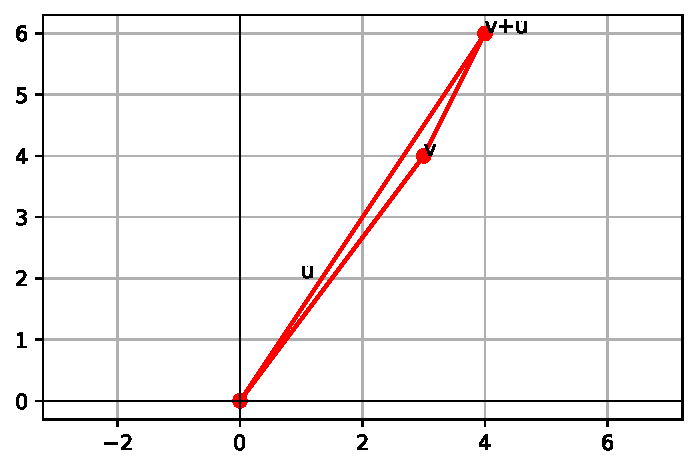
\includegraphics[keepaspectratio]{books/en-US/lab_files/figure-latex/cell-50-output-1.pdf}}

This triangle shows why the inequality is called the ``triangle''
inequality.

\begin{enumerate}
\def\labelenumi{\arabic{enumi}.}
\setcounter{enumi}{4}
\tightlist
\item
  Testing triangle inequality with random vectors
\end{enumerate}

\begin{Shaded}
\begin{Highlighting}[]
\ControlFlowTok{for}\NormalTok{ \_ }\KeywordTok{in} \BuiltInTok{range}\NormalTok{(}\DecValTok{5}\NormalTok{):}
\NormalTok{    v }\OperatorTok{=}\NormalTok{ np.random.randn(}\DecValTok{2}\NormalTok{)}
\NormalTok{    u }\OperatorTok{=}\NormalTok{ np.random.randn(}\DecValTok{2}\NormalTok{)}
\NormalTok{    lhs }\OperatorTok{=}\NormalTok{ np.linalg.norm(v}\OperatorTok{+}\NormalTok{u)}
\NormalTok{    rhs }\OperatorTok{=}\NormalTok{ np.linalg.norm(v) }\OperatorTok{+}\NormalTok{ np.linalg.norm(u)}
    \BuiltInTok{print}\NormalTok{(}\SpecialStringTok{f"‖v+u‖=}\SpecialCharTok{\{}\NormalTok{lhs}\SpecialCharTok{:.3f\}}\SpecialStringTok{, ‖v‖+‖u‖=}\SpecialCharTok{\{}\NormalTok{rhs}\SpecialCharTok{:.3f\}}\SpecialStringTok{, holds=}\SpecialCharTok{\{}\NormalTok{lhs }\OperatorTok{\textless{}=}\NormalTok{ rhs}\SpecialCharTok{\}}\SpecialStringTok{"}\NormalTok{)}
\end{Highlighting}
\end{Shaded}

\begin{verbatim}
‖v+u‖=0.778, ‖v‖+‖u‖=2.112, holds=True
‖v+u‖=1.040, ‖v‖+‖u‖=2.621, holds=True
‖v+u‖=1.632, ‖v‖+‖u‖=2.482, holds=True
‖v+u‖=1.493, ‖v‖+‖u‖=2.250, holds=True
‖v+u‖=2.653, ‖v‖+‖u‖=2.692, holds=True
\end{verbatim}

No matter what vectors you try, the inequality always holds.

\subsubsection{The Takeaway}\label{the-takeaway}

\begin{itemize}
\tightlist
\item
  Cauchy--Schwarz: The dot product is always bounded by the product of
  vector lengths.
\item
  Triangle inequality: The length of one side of a triangle can't exceed
  the sum of the other two.
\item
  These inequalities form the backbone of geometry, analysis, and many
  proofs in linear algebra.
\end{itemize}

\subsection{10. Orthonormal Sets in
ℝ²/ℝ³}\label{orthonormal-sets-in-ux211duxb2ux211duxb3}

In this lab, we'll explore orthonormal sets - collections of vectors
that are both orthogonal (perpendicular) and normalized (length = 1).
These sets are the ``nicest'' possible bases for vector spaces. In 2D
and 3D, they correspond to the coordinate axes we already know, but we
can also construct and test new ones.

\subsubsection{Set Up Your Lab}\label{set-up-your-lab-9}

\begin{Shaded}
\begin{Highlighting}[]
\ImportTok{import}\NormalTok{ numpy }\ImportTok{as}\NormalTok{ np}
\ImportTok{import}\NormalTok{ matplotlib.pyplot }\ImportTok{as}\NormalTok{ plt}
\end{Highlighting}
\end{Shaded}

\subsubsection{Step-by-Step Code
Walkthrough}\label{step-by-step-code-walkthrough-9}

\begin{enumerate}
\def\labelenumi{\arabic{enumi}.}
\tightlist
\item
  Orthogonal vectors Two vectors are orthogonal if their dot product is
  zero.
\end{enumerate}

\begin{Shaded}
\begin{Highlighting}[]
\NormalTok{x\_axis }\OperatorTok{=}\NormalTok{ np.array([}\DecValTok{1}\NormalTok{, }\DecValTok{0}\NormalTok{])}
\NormalTok{y\_axis }\OperatorTok{=}\NormalTok{ np.array([}\DecValTok{0}\NormalTok{, }\DecValTok{1}\NormalTok{])}

\BuiltInTok{print}\NormalTok{(}\StringTok{"x\_axis · y\_axis ="}\NormalTok{, np.dot(x\_axis, y\_axis))  }\CommentTok{\# should be 0}
\end{Highlighting}
\end{Shaded}

\begin{verbatim}
x_axis · y_axis = 0
\end{verbatim}

So the standard axes are orthogonal.

\begin{enumerate}
\def\labelenumi{\arabic{enumi}.}
\setcounter{enumi}{1}
\tightlist
\item
  Normalizing vectors Normalization means dividing a vector by its
  length to make its norm equal to 1.
\end{enumerate}

\begin{Shaded}
\begin{Highlighting}[]
\NormalTok{v }\OperatorTok{=}\NormalTok{ np.array([}\DecValTok{3}\NormalTok{, }\DecValTok{4}\NormalTok{])}
\NormalTok{v\_normalized }\OperatorTok{=}\NormalTok{ v }\OperatorTok{/}\NormalTok{ np.linalg.norm(v)}

\BuiltInTok{print}\NormalTok{(}\StringTok{"Original v:"}\NormalTok{, v)}
\BuiltInTok{print}\NormalTok{(}\StringTok{"Normalized v:"}\NormalTok{, v\_normalized)}
\BuiltInTok{print}\NormalTok{(}\StringTok{"Length of normalized v:"}\NormalTok{, np.linalg.norm(v\_normalized))}
\end{Highlighting}
\end{Shaded}

\begin{verbatim}
Original v: [3 4]
Normalized v: [0.6 0.8]
Length of normalized v: 1.0
\end{verbatim}

Now \texttt{v\_normalized} points in the same direction as \texttt{v}
but has unit length.

\begin{enumerate}
\def\labelenumi{\arabic{enumi}.}
\setcounter{enumi}{2}
\tightlist
\item
  Building an orthonormal set in 2D
\end{enumerate}

\begin{Shaded}
\begin{Highlighting}[]
\NormalTok{u1 }\OperatorTok{=}\NormalTok{ np.array([}\DecValTok{1}\NormalTok{, }\DecValTok{0}\NormalTok{])}
\NormalTok{u2 }\OperatorTok{=}\NormalTok{ np.array([}\DecValTok{0}\NormalTok{, }\DecValTok{1}\NormalTok{])}

\BuiltInTok{print}\NormalTok{(}\StringTok{"u1 length:"}\NormalTok{, np.linalg.norm(u1))}
\BuiltInTok{print}\NormalTok{(}\StringTok{"u2 length:"}\NormalTok{, np.linalg.norm(u2))}
\BuiltInTok{print}\NormalTok{(}\StringTok{"u1 · u2 ="}\NormalTok{, np.dot(u1,u2))}
\end{Highlighting}
\end{Shaded}

\begin{verbatim}
u1 length: 1.0
u2 length: 1.0
u1 · u2 = 0
\end{verbatim}

Both have length 1, and their dot product is 0. That makes
\texttt{\{u1,\ u2\}} an orthonormal set in 2D.

\begin{enumerate}
\def\labelenumi{\arabic{enumi}.}
\setcounter{enumi}{3}
\tightlist
\item
  Visualizing 2D orthonormal vectors
\end{enumerate}

\begin{Shaded}
\begin{Highlighting}[]
\NormalTok{plt.quiver(}\DecValTok{0}\NormalTok{,}\DecValTok{0}\NormalTok{,u1[}\DecValTok{0}\NormalTok{],u1[}\DecValTok{1}\NormalTok{],angles}\OperatorTok{=}\StringTok{\textquotesingle{}xy\textquotesingle{}}\NormalTok{,scale\_units}\OperatorTok{=}\StringTok{\textquotesingle{}xy\textquotesingle{}}\NormalTok{,scale}\OperatorTok{=}\DecValTok{1}\NormalTok{,color}\OperatorTok{=}\StringTok{\textquotesingle{}r\textquotesingle{}}\NormalTok{)}
\NormalTok{plt.quiver(}\DecValTok{0}\NormalTok{,}\DecValTok{0}\NormalTok{,u2[}\DecValTok{0}\NormalTok{],u2[}\DecValTok{1}\NormalTok{],angles}\OperatorTok{=}\StringTok{\textquotesingle{}xy\textquotesingle{}}\NormalTok{,scale\_units}\OperatorTok{=}\StringTok{\textquotesingle{}xy\textquotesingle{}}\NormalTok{,scale}\OperatorTok{=}\DecValTok{1}\NormalTok{,color}\OperatorTok{=}\StringTok{\textquotesingle{}b\textquotesingle{}}\NormalTok{)}

\NormalTok{plt.xlim(}\OperatorTok{{-}}\FloatTok{1.5}\NormalTok{,}\FloatTok{1.5}\NormalTok{)}
\NormalTok{plt.ylim(}\OperatorTok{{-}}\FloatTok{1.5}\NormalTok{,}\FloatTok{1.5}\NormalTok{)}
\NormalTok{plt.axhline(}\DecValTok{0}\NormalTok{,color}\OperatorTok{=}\StringTok{\textquotesingle{}black\textquotesingle{}}\NormalTok{,linewidth}\OperatorTok{=}\FloatTok{0.5}\NormalTok{)}
\NormalTok{plt.axvline(}\DecValTok{0}\NormalTok{,color}\OperatorTok{=}\StringTok{\textquotesingle{}black\textquotesingle{}}\NormalTok{,linewidth}\OperatorTok{=}\FloatTok{0.5}\NormalTok{)}
\NormalTok{plt.grid()}
\NormalTok{plt.show()}
\end{Highlighting}
\end{Shaded}

\pandocbounded{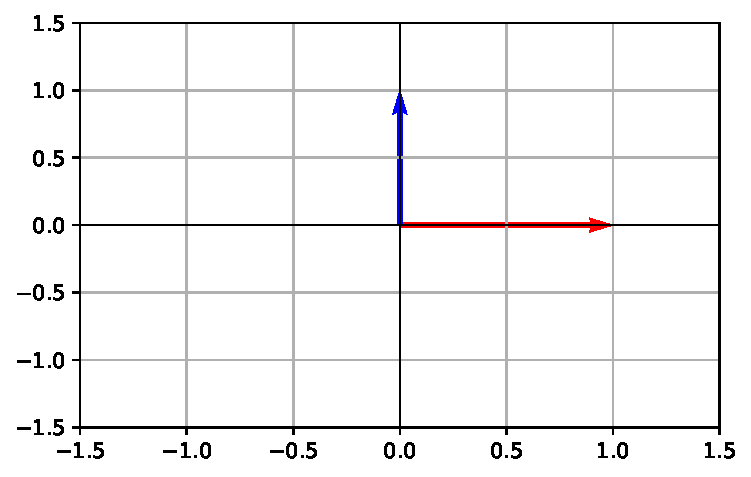
\includegraphics[keepaspectratio]{books/en-US/lab_files/figure-latex/cell-56-output-1.pdf}}

You'll see the red and blue arrows at right angles, each of length 1.

\begin{enumerate}
\def\labelenumi{\arabic{enumi}.}
\setcounter{enumi}{4}
\tightlist
\item
  Orthonormal set in 3D In 3D, the standard basis vectors are:
\end{enumerate}

\begin{Shaded}
\begin{Highlighting}[]
\NormalTok{i }\OperatorTok{=}\NormalTok{ np.array([}\DecValTok{1}\NormalTok{,}\DecValTok{0}\NormalTok{,}\DecValTok{0}\NormalTok{])}
\NormalTok{j }\OperatorTok{=}\NormalTok{ np.array([}\DecValTok{0}\NormalTok{,}\DecValTok{1}\NormalTok{,}\DecValTok{0}\NormalTok{])}
\NormalTok{k }\OperatorTok{=}\NormalTok{ np.array([}\DecValTok{0}\NormalTok{,}\DecValTok{0}\NormalTok{,}\DecValTok{1}\NormalTok{])}

\BuiltInTok{print}\NormalTok{(}\StringTok{"‖i‖ ="}\NormalTok{, np.linalg.norm(i))}
\BuiltInTok{print}\NormalTok{(}\StringTok{"‖j‖ ="}\NormalTok{, np.linalg.norm(j))}
\BuiltInTok{print}\NormalTok{(}\StringTok{"‖k‖ ="}\NormalTok{, np.linalg.norm(k))}
\BuiltInTok{print}\NormalTok{(}\StringTok{"i·j ="}\NormalTok{, np.dot(i,j))}
\BuiltInTok{print}\NormalTok{(}\StringTok{"j·k ="}\NormalTok{, np.dot(j,k))}
\BuiltInTok{print}\NormalTok{(}\StringTok{"i·k ="}\NormalTok{, np.dot(i,k))}
\end{Highlighting}
\end{Shaded}

\begin{verbatim}
‖i‖ = 1.0
‖j‖ = 1.0
‖k‖ = 1.0
i·j = 0
j·k = 0
i·k = 0
\end{verbatim}

Lengths are all 1, and dot products are 0. So \texttt{\{i,\ j,\ k\}} is
an orthonormal set in ℝ³.

\begin{enumerate}
\def\labelenumi{\arabic{enumi}.}
\setcounter{enumi}{5}
\tightlist
\item
  Testing if a set is orthonormal We can write a helper function:
\end{enumerate}

\begin{Shaded}
\begin{Highlighting}[]
\KeywordTok{def}\NormalTok{ is\_orthonormal(vectors):}
    \ControlFlowTok{for}\NormalTok{ i }\KeywordTok{in} \BuiltInTok{range}\NormalTok{(}\BuiltInTok{len}\NormalTok{(vectors)):}
        \ControlFlowTok{for}\NormalTok{ j }\KeywordTok{in} \BuiltInTok{range}\NormalTok{(}\BuiltInTok{len}\NormalTok{(vectors)):}
\NormalTok{            dot }\OperatorTok{=}\NormalTok{ np.dot(vectors[i], vectors[j])}
            \ControlFlowTok{if}\NormalTok{ i }\OperatorTok{==}\NormalTok{ j:}
                \ControlFlowTok{if} \KeywordTok{not}\NormalTok{ np.isclose(dot, }\DecValTok{1}\NormalTok{): }\ControlFlowTok{return} \VariableTok{False}
            \ControlFlowTok{else}\NormalTok{:}
                \ControlFlowTok{if} \KeywordTok{not}\NormalTok{ np.isclose(dot, }\DecValTok{0}\NormalTok{): }\ControlFlowTok{return} \VariableTok{False}
    \ControlFlowTok{return} \VariableTok{True}

\BuiltInTok{print}\NormalTok{(is\_orthonormal([i, j, k]))  }\CommentTok{\# True}
\end{Highlighting}
\end{Shaded}

\begin{verbatim}
True
\end{verbatim}

\begin{enumerate}
\def\labelenumi{\arabic{enumi}.}
\setcounter{enumi}{6}
\tightlist
\item
  Constructing a new orthonormal pair Not all orthonormal sets look like
  the axes.
\end{enumerate}

\begin{Shaded}
\begin{Highlighting}[]
\NormalTok{u1 }\OperatorTok{=}\NormalTok{ np.array([}\DecValTok{1}\NormalTok{,}\DecValTok{1}\NormalTok{]) }\OperatorTok{/}\NormalTok{ np.sqrt(}\DecValTok{2}\NormalTok{)}
\NormalTok{u2 }\OperatorTok{=}\NormalTok{ np.array([}\OperatorTok{{-}}\DecValTok{1}\NormalTok{,}\DecValTok{1}\NormalTok{]) }\OperatorTok{/}\NormalTok{ np.sqrt(}\DecValTok{2}\NormalTok{)}

\BuiltInTok{print}\NormalTok{(}\StringTok{"u1·u2 ="}\NormalTok{, np.dot(u1,u2))}
\BuiltInTok{print}\NormalTok{(}\StringTok{"‖u1‖ ="}\NormalTok{, np.linalg.norm(u1))}
\BuiltInTok{print}\NormalTok{(}\StringTok{"‖u2‖ ="}\NormalTok{, np.linalg.norm(u2))}
\end{Highlighting}
\end{Shaded}

\begin{verbatim}
u1·u2 = 0.0
‖u1‖ = 0.9999999999999999
‖u2‖ = 0.9999999999999999
\end{verbatim}

This gives a rotated orthonormal basis in 2D.

\subsubsection{Try It Yourself}\label{try-it-yourself-108}

\begin{enumerate}
\def\labelenumi{\arabic{enumi}.}
\tightlist
\item
  Normalize \texttt{(2,2,1)} to make it a unit vector.
\item
  Test whether the set
  \texttt{\{{[}1,0,0{]},\ {[}0,2,0{]},\ {[}0,0,3{]}\}} is orthonormal.
\item
  Construct two vectors in 2D that are not perpendicular. Normalize them
  and check if the dot product is still zero.
\end{enumerate}

\section{Chapter 2. Matrices and basic
operations}\label{chapter-2.-matrices-and-basic-operations-2}

\subsection{11. Matrices as Tables and as
Machines}\label{matrices-as-tables-and-as-machines-1}

Matrices can feel mysterious at first, but there are two simple ways to
think about them:

\begin{enumerate}
\def\labelenumi{\arabic{enumi}.}
\tightlist
\item
  As tables of numbers - just a grid you can store and manipulate.
\item
  As machines - something that takes a vector in and spits a new vector
  out.
\end{enumerate}

In this lab, we'll explore both views and see how they connect.

\subsubsection{Set Up Your Lab}\label{set-up-your-lab-10}

\begin{Shaded}
\begin{Highlighting}[]
\ImportTok{import}\NormalTok{ numpy }\ImportTok{as}\NormalTok{ np}
\end{Highlighting}
\end{Shaded}

\subsubsection{Step-by-Step Code
Walkthrough}\label{step-by-step-code-walkthrough-10}

\begin{enumerate}
\def\labelenumi{\arabic{enumi}.}
\tightlist
\item
  A matrix as a table of numbers
\end{enumerate}

\begin{Shaded}
\begin{Highlighting}[]
\NormalTok{A }\OperatorTok{=}\NormalTok{ np.array([}
\NormalTok{    [}\DecValTok{1}\NormalTok{, }\DecValTok{2}\NormalTok{, }\DecValTok{3}\NormalTok{],}
\NormalTok{    [}\DecValTok{4}\NormalTok{, }\DecValTok{5}\NormalTok{, }\DecValTok{6}\NormalTok{]}
\NormalTok{])}

\BuiltInTok{print}\NormalTok{(}\StringTok{"Matrix A:}\CharTok{\textbackslash{}n}\StringTok{"}\NormalTok{, A)}
\BuiltInTok{print}\NormalTok{(}\StringTok{"Shape of A:"}\NormalTok{, A.shape)}
\end{Highlighting}
\end{Shaded}

\begin{verbatim}
Matrix A:
 [[1 2 3]
 [4 5 6]]
Shape of A: (2, 3)
\end{verbatim}

Here, \texttt{A} is a 2×3 matrix (2 rows, 3 columns).

\begin{itemize}
\tightlist
\item
  Rows = horizontal slices → \texttt{{[}1,2,3{]}} and
  \texttt{{[}4,5,6{]}}
\item
  Columns = vertical slices → \texttt{{[}1,4{]}}, \texttt{{[}2,5{]}},
  \texttt{{[}3,6{]}}
\end{itemize}

\begin{enumerate}
\def\labelenumi{\arabic{enumi}.}
\setcounter{enumi}{1}
\tightlist
\item
  Accessing rows and columns
\end{enumerate}

\begin{Shaded}
\begin{Highlighting}[]
\NormalTok{first\_row }\OperatorTok{=}\NormalTok{ A[}\DecValTok{0}\NormalTok{]        }\CommentTok{\# row 0}
\NormalTok{second\_column }\OperatorTok{=}\NormalTok{ A[:,}\DecValTok{1}\NormalTok{]  }\CommentTok{\# column 1}

\BuiltInTok{print}\NormalTok{(}\StringTok{"First row:"}\NormalTok{, first\_row)}
\BuiltInTok{print}\NormalTok{(}\StringTok{"Second column:"}\NormalTok{, second\_column)}
\end{Highlighting}
\end{Shaded}

\begin{verbatim}
First row: [1 2 3]
Second column: [2 5]
\end{verbatim}

Rows are whole vectors too, and so are columns.

\begin{enumerate}
\def\labelenumi{\arabic{enumi}.}
\setcounter{enumi}{2}
\tightlist
\item
  A matrix as a machine
\end{enumerate}

A matrix can ``act'' on a vector. If \texttt{x\ =\ {[}x1,\ x2,\ x3{]}},
then \texttt{A·x} is computed by taking linear combinations of the
columns of \texttt{A}.

\begin{Shaded}
\begin{Highlighting}[]
\NormalTok{x }\OperatorTok{=}\NormalTok{ np.array([}\DecValTok{1}\NormalTok{, }\DecValTok{0}\NormalTok{, }\OperatorTok{{-}}\DecValTok{1}\NormalTok{])  }\CommentTok{\# a 3D vector}
\NormalTok{result }\OperatorTok{=}\NormalTok{ A.dot(x)}

\BuiltInTok{print}\NormalTok{(}\StringTok{"A·x ="}\NormalTok{, result)}
\end{Highlighting}
\end{Shaded}

\begin{verbatim}
A·x = [-2 -2]
\end{verbatim}

Interpretation: multiply \texttt{A} by \texttt{x} = combine columns of
\texttt{A} with weights from \texttt{x}.

\[
A \cdot x = 1 \cdot \text{(col 1)} + 0 \cdot \text{(col 2)} + (-1) \cdot \text{(col 3)}
\]

\begin{enumerate}
\def\labelenumi{\arabic{enumi}.}
\setcounter{enumi}{3}
\tightlist
\item
  Verifying column combination view
\end{enumerate}

\begin{Shaded}
\begin{Highlighting}[]
\NormalTok{col1 }\OperatorTok{=}\NormalTok{ A[:,}\DecValTok{0}\NormalTok{]}
\NormalTok{col2 }\OperatorTok{=}\NormalTok{ A[:,}\DecValTok{1}\NormalTok{]}
\NormalTok{col3 }\OperatorTok{=}\NormalTok{ A[:,}\DecValTok{2}\NormalTok{]}

\NormalTok{manual }\OperatorTok{=} \DecValTok{1}\OperatorTok{*}\NormalTok{col1 }\OperatorTok{+} \DecValTok{0}\OperatorTok{*}\NormalTok{col2 }\OperatorTok{+}\NormalTok{ (}\OperatorTok{{-}}\DecValTok{1}\NormalTok{)}\OperatorTok{*}\NormalTok{col3}
\BuiltInTok{print}\NormalTok{(}\StringTok{"Manual combination:"}\NormalTok{, manual)}
\BuiltInTok{print}\NormalTok{(}\StringTok{"A·x result:"}\NormalTok{, result)}
\end{Highlighting}
\end{Shaded}

\begin{verbatim}
Manual combination: [-2 -2]
A·x result: [-2 -2]
\end{verbatim}

They match exactly. This shows the ``machine'' interpretation is just a
shortcut for column combinations.

\begin{enumerate}
\def\labelenumi{\arabic{enumi}.}
\setcounter{enumi}{4}
\tightlist
\item
  Geometric intuition (2D example)
\end{enumerate}

\begin{Shaded}
\begin{Highlighting}[]
\NormalTok{B }\OperatorTok{=}\NormalTok{ np.array([}
\NormalTok{    [}\DecValTok{2}\NormalTok{, }\DecValTok{0}\NormalTok{],}
\NormalTok{    [}\DecValTok{0}\NormalTok{, }\DecValTok{1}\NormalTok{]}
\NormalTok{])}

\NormalTok{v }\OperatorTok{=}\NormalTok{ np.array([}\DecValTok{1}\NormalTok{,}\DecValTok{2}\NormalTok{])}
\BuiltInTok{print}\NormalTok{(}\StringTok{"B·v ="}\NormalTok{, B.dot(v))}
\end{Highlighting}
\end{Shaded}

\begin{verbatim}
B·v = [2 2]
\end{verbatim}

Here, \texttt{B} scales the x-direction by 2 while leaving the
y-direction alone. So \texttt{(1,2)} becomes \texttt{(2,2)}.

\subsubsection{Try It Yourself}\label{try-it-yourself-109}

\begin{enumerate}
\def\labelenumi{\arabic{enumi}.}
\tightlist
\item
  Create a 3×3 identity matrix with \texttt{np.eye(3)} and multiply it
  by different vectors. What happens?
\item
  Build a matrix \texttt{{[}{[}0,-1{]},{[}1,0{]}{]}}. Try multiplying it
  by \texttt{(1,0)} and \texttt{(0,1)}. What transformation is this?
\item
  Create your own 2×2 matrix that flips vectors across the x-axis. Test
  it on \texttt{(1,2)} and \texttt{(−3,4)}.
\end{enumerate}

\subsubsection{The Takeaway}\label{the-takeaway-1}

\begin{itemize}
\tightlist
\item
  A matrix is both a grid of numbers and a machine that transforms
  vectors.
\item
  Matrix--vector multiplication is the same as combining columns with
  given weights.
\item
  Thinking of matrices as machines helps build intuition for rotations,
  scalings, and other transformations later.
\end{itemize}

\subsection{12. Matrix Shapes, Indexing, and Block
Views}\label{matrix-shapes-indexing-and-block-views-1}

Matrices come in many shapes, and learning to read their structure is
essential. Shape tells us how many rows and columns a matrix has.
Indexing lets us grab specific entries, rows, or columns. Block views
let us zoom in on submatrices, which is extremely useful for both theory
and computation.

\subsubsection{Set Up Your Lab}\label{set-up-your-lab-11}

\begin{Shaded}
\begin{Highlighting}[]
\ImportTok{import}\NormalTok{ numpy }\ImportTok{as}\NormalTok{ np}
\end{Highlighting}
\end{Shaded}

\subsubsection{Step-by-Step Code
Walkthrough}\label{step-by-step-code-walkthrough-11}

\begin{enumerate}
\def\labelenumi{\arabic{enumi}.}
\tightlist
\item
  Matrix shapes
\end{enumerate}

The shape of a matrix is \texttt{(rows,\ columns)}.

\begin{Shaded}
\begin{Highlighting}[]
\NormalTok{A }\OperatorTok{=}\NormalTok{ np.array([}
\NormalTok{    [}\DecValTok{1}\NormalTok{, }\DecValTok{2}\NormalTok{, }\DecValTok{3}\NormalTok{],}
\NormalTok{    [}\DecValTok{4}\NormalTok{, }\DecValTok{5}\NormalTok{, }\DecValTok{6}\NormalTok{],}
\NormalTok{    [}\DecValTok{7}\NormalTok{, }\DecValTok{8}\NormalTok{, }\DecValTok{9}\NormalTok{]}
\NormalTok{])}

\BuiltInTok{print}\NormalTok{(}\StringTok{"Matrix A:}\CharTok{\textbackslash{}n}\StringTok{"}\NormalTok{, A)}
\BuiltInTok{print}\NormalTok{(}\StringTok{"Shape of A:"}\NormalTok{, A.shape)}
\end{Highlighting}
\end{Shaded}

\begin{verbatim}
Matrix A:
 [[1 2 3]
 [4 5 6]
 [7 8 9]]
Shape of A: (3, 3)
\end{verbatim}

Here, \texttt{A} is a 3×3 matrix.

\begin{enumerate}
\def\labelenumi{\arabic{enumi}.}
\setcounter{enumi}{1}
\tightlist
\item
  Indexing elements
\end{enumerate}

In NumPy, rows and columns are 0-based. The first entry is
\texttt{A{[}0,0{]}}.

\begin{Shaded}
\begin{Highlighting}[]
\BuiltInTok{print}\NormalTok{(}\StringTok{"A[0,0] ="}\NormalTok{, A[}\DecValTok{0}\NormalTok{,}\DecValTok{0}\NormalTok{])  }\CommentTok{\# top{-}left element}
\BuiltInTok{print}\NormalTok{(}\StringTok{"A[1,2] ="}\NormalTok{, A[}\DecValTok{1}\NormalTok{,}\DecValTok{2}\NormalTok{])  }\CommentTok{\# second row, third column}
\end{Highlighting}
\end{Shaded}

\begin{verbatim}
A[0,0] = 1
A[1,2] = 6
\end{verbatim}

\begin{enumerate}
\def\labelenumi{\arabic{enumi}.}
\setcounter{enumi}{2}
\tightlist
\item
  Extracting rows and columns
\end{enumerate}

\begin{Shaded}
\begin{Highlighting}[]
\NormalTok{row1 }\OperatorTok{=}\NormalTok{ A[}\DecValTok{0}\NormalTok{]       }\CommentTok{\# first row}
\NormalTok{col2 }\OperatorTok{=}\NormalTok{ A[:,}\DecValTok{1}\NormalTok{]     }\CommentTok{\# second column}

\BuiltInTok{print}\NormalTok{(}\StringTok{"First row:"}\NormalTok{, row1)}
\BuiltInTok{print}\NormalTok{(}\StringTok{"Second column:"}\NormalTok{, col2)}
\end{Highlighting}
\end{Shaded}

\begin{verbatim}
First row: [1 2 3]
Second column: [2 5 8]
\end{verbatim}

Notice: \texttt{A{[}i{]}} gives a row, \texttt{A{[}:,j{]}} gives a
column.

\begin{enumerate}
\def\labelenumi{\arabic{enumi}.}
\setcounter{enumi}{3}
\tightlist
\item
  Slicing submatrices (block view)
\end{enumerate}

You can slice multiple rows and columns to form a smaller matrix.

\begin{Shaded}
\begin{Highlighting}[]
\NormalTok{block }\OperatorTok{=}\NormalTok{ A[}\DecValTok{0}\NormalTok{:}\DecValTok{2}\NormalTok{, }\DecValTok{1}\NormalTok{:}\DecValTok{3}\NormalTok{]  }\CommentTok{\# rows 0–1, columns 1–2}
\BuiltInTok{print}\NormalTok{(}\StringTok{"Block submatrix:}\CharTok{\textbackslash{}n}\StringTok{"}\NormalTok{, block)}
\end{Highlighting}
\end{Shaded}

\begin{verbatim}
Block submatrix:
 [[2 3]
 [5 6]]
\end{verbatim}

This block is:

\[
\begin{bmatrix}
2 & 3 \\
5 & 6
\end{bmatrix}
\]

\begin{enumerate}
\def\labelenumi{\arabic{enumi}.}
\setcounter{enumi}{4}
\tightlist
\item
  Modifying parts of a matrix
\end{enumerate}

\begin{Shaded}
\begin{Highlighting}[]
\NormalTok{A[}\DecValTok{0}\NormalTok{,}\DecValTok{0}\NormalTok{] }\OperatorTok{=} \DecValTok{99}
\BuiltInTok{print}\NormalTok{(}\StringTok{"Modified A:}\CharTok{\textbackslash{}n}\StringTok{"}\NormalTok{, A)}

\NormalTok{A[}\DecValTok{1}\NormalTok{,:] }\OperatorTok{=}\NormalTok{ [}\DecValTok{10}\NormalTok{, }\DecValTok{11}\NormalTok{, }\DecValTok{12}\NormalTok{]   }\CommentTok{\# replace row 1}
\BuiltInTok{print}\NormalTok{(}\StringTok{"After replacing row 1:}\CharTok{\textbackslash{}n}\StringTok{"}\NormalTok{, A)}
\end{Highlighting}
\end{Shaded}

\begin{verbatim}
Modified A:
 [[99  2  3]
 [ 4  5  6]
 [ 7  8  9]]
After replacing row 1:
 [[99  2  3]
 [10 11 12]
 [ 7  8  9]]
\end{verbatim}

\begin{enumerate}
\def\labelenumi{\arabic{enumi}.}
\setcounter{enumi}{5}
\tightlist
\item
  Non-square matrices
\end{enumerate}

Not all matrices are square. Shapes can be rectangular, too.

\begin{Shaded}
\begin{Highlighting}[]
\NormalTok{B }\OperatorTok{=}\NormalTok{ np.array([}
\NormalTok{    [}\DecValTok{1}\NormalTok{, }\DecValTok{2}\NormalTok{],}
\NormalTok{    [}\DecValTok{3}\NormalTok{, }\DecValTok{4}\NormalTok{],}
\NormalTok{    [}\DecValTok{5}\NormalTok{, }\DecValTok{6}\NormalTok{]}
\NormalTok{])}

\BuiltInTok{print}\NormalTok{(}\StringTok{"Matrix B:}\CharTok{\textbackslash{}n}\StringTok{"}\NormalTok{, B)}
\BuiltInTok{print}\NormalTok{(}\StringTok{"Shape of B:"}\NormalTok{, B.shape)}
\end{Highlighting}
\end{Shaded}

\begin{verbatim}
Matrix B:
 [[1 2]
 [3 4]
 [5 6]]
Shape of B: (3, 2)
\end{verbatim}

Here, \texttt{B} is 3×2 (3 rows, 2 columns).

\begin{enumerate}
\def\labelenumi{\arabic{enumi}.}
\setcounter{enumi}{6}
\tightlist
\item
  Block decomposition idea
\end{enumerate}

We can think of large matrices as made of smaller blocks. This is common
in linear algebra proofs and algorithms.

\begin{Shaded}
\begin{Highlighting}[]
\NormalTok{C }\OperatorTok{=}\NormalTok{ np.array([}
\NormalTok{    [}\DecValTok{1}\NormalTok{,}\DecValTok{2}\NormalTok{,}\DecValTok{3}\NormalTok{,}\DecValTok{4}\NormalTok{],}
\NormalTok{    [}\DecValTok{5}\NormalTok{,}\DecValTok{6}\NormalTok{,}\DecValTok{7}\NormalTok{,}\DecValTok{8}\NormalTok{],}
\NormalTok{    [}\DecValTok{9}\NormalTok{,}\DecValTok{10}\NormalTok{,}\DecValTok{11}\NormalTok{,}\DecValTok{12}\NormalTok{],}
\NormalTok{    [}\DecValTok{13}\NormalTok{,}\DecValTok{14}\NormalTok{,}\DecValTok{15}\NormalTok{,}\DecValTok{16}\NormalTok{]}
\NormalTok{])}

\NormalTok{top\_left }\OperatorTok{=}\NormalTok{ C[}\DecValTok{0}\NormalTok{:}\DecValTok{2}\NormalTok{, }\DecValTok{0}\NormalTok{:}\DecValTok{2}\NormalTok{]}
\NormalTok{bottom\_right }\OperatorTok{=}\NormalTok{ C[}\DecValTok{2}\NormalTok{:}\DecValTok{4}\NormalTok{, }\DecValTok{2}\NormalTok{:}\DecValTok{4}\NormalTok{]}

\BuiltInTok{print}\NormalTok{(}\StringTok{"Top{-}left block:}\CharTok{\textbackslash{}n}\StringTok{"}\NormalTok{, top\_left)}
\BuiltInTok{print}\NormalTok{(}\StringTok{"Bottom{-}right block:}\CharTok{\textbackslash{}n}\StringTok{"}\NormalTok{, bottom\_right)}
\end{Highlighting}
\end{Shaded}

\begin{verbatim}
Top-left block:
 [[1 2]
 [5 6]]
Bottom-right block:
 [[11 12]
 [15 16]]
\end{verbatim}

This is the start of block matrix notation.

\subsubsection{Try It Yourself}\label{try-it-yourself-110}

\begin{enumerate}
\def\labelenumi{\arabic{enumi}.}
\tightlist
\item
  Create a 4×5 matrix with values 1--20 using
  \texttt{np.arange(1,21).reshape(4,5)}. Find its shape.
\item
  Extract the middle row and last column.
\item
  Cut it into four 2×2 blocks. Can you reassemble them in a different
  order?
\end{enumerate}

\subsection{13. Matrix Addition and Scalar
Multiplication}\label{matrix-addition-and-scalar-multiplication-1}

Now that we understand matrix shapes and indexing, let's practice two of
the simplest but most important operations: adding matrices and scaling
them with numbers (scalars). These operations extend the rules we
already know for vectors.

\subsubsection{Set Up Your Lab}\label{set-up-your-lab-12}

\begin{Shaded}
\begin{Highlighting}[]
\ImportTok{import}\NormalTok{ numpy }\ImportTok{as}\NormalTok{ np}
\end{Highlighting}
\end{Shaded}

\subsubsection{Step-by-Step Code
Walkthrough}\label{step-by-step-code-walkthrough-12}

\begin{enumerate}
\def\labelenumi{\arabic{enumi}.}
\tightlist
\item
  Adding two matrices You can add two matrices if (and only if) they
  have the same shape. Addition happens entry by entry.
\end{enumerate}

\begin{Shaded}
\begin{Highlighting}[]
\NormalTok{A }\OperatorTok{=}\NormalTok{ np.array([}
\NormalTok{    [}\DecValTok{1}\NormalTok{, }\DecValTok{2}\NormalTok{],}
\NormalTok{    [}\DecValTok{3}\NormalTok{, }\DecValTok{4}\NormalTok{]}
\NormalTok{])}

\NormalTok{B }\OperatorTok{=}\NormalTok{ np.array([}
\NormalTok{    [}\DecValTok{5}\NormalTok{, }\DecValTok{6}\NormalTok{],}
\NormalTok{    [}\DecValTok{7}\NormalTok{, }\DecValTok{8}\NormalTok{]}
\NormalTok{])}

\NormalTok{C }\OperatorTok{=}\NormalTok{ A }\OperatorTok{+}\NormalTok{ B}
\BuiltInTok{print}\NormalTok{(}\StringTok{"A + B =}\CharTok{\textbackslash{}n}\StringTok{"}\NormalTok{, C)}
\end{Highlighting}
\end{Shaded}

\begin{verbatim}
A + B =
 [[ 6  8]
 [10 12]]
\end{verbatim}

Each element in \texttt{C} is the sum of corresponding elements in
\texttt{A} and \texttt{B}.

\begin{enumerate}
\def\labelenumi{\arabic{enumi}.}
\setcounter{enumi}{1}
\tightlist
\item
  Scalar multiplication Multiplying a matrix by a scalar multiplies
  every entry by that number.
\end{enumerate}

\begin{Shaded}
\begin{Highlighting}[]
\NormalTok{k }\OperatorTok{=} \DecValTok{3}
\NormalTok{D }\OperatorTok{=}\NormalTok{ k }\OperatorTok{*}\NormalTok{ A}
\BuiltInTok{print}\NormalTok{(}\StringTok{"3 * A =}\CharTok{\textbackslash{}n}\StringTok{"}\NormalTok{, D)}
\end{Highlighting}
\end{Shaded}

\begin{verbatim}
3 * A =
 [[ 3  6]
 [ 9 12]]
\end{verbatim}

Here, each element of \texttt{A} is tripled.

\begin{enumerate}
\def\labelenumi{\arabic{enumi}.}
\setcounter{enumi}{2}
\tightlist
\item
  Combining both operations We can mix addition and scaling, just like
  with vectors.
\end{enumerate}

\begin{Shaded}
\begin{Highlighting}[]
\NormalTok{combo }\OperatorTok{=} \DecValTok{2}\OperatorTok{*}\NormalTok{A }\OperatorTok{{-}}\NormalTok{ B}
\BuiltInTok{print}\NormalTok{(}\StringTok{"2A {-} B =}\CharTok{\textbackslash{}n}\StringTok{"}\NormalTok{, combo)}
\end{Highlighting}
\end{Shaded}

\begin{verbatim}
2A - B =
 [[-3 -2]
 [-1  0]]
\end{verbatim}

This creates new matrices as linear combinations of others.

\begin{enumerate}
\def\labelenumi{\arabic{enumi}.}
\setcounter{enumi}{3}
\tightlist
\item
  Zero matrix A matrix of all zeros acts like ``nothing happens'' for
  addition.
\end{enumerate}

\begin{Shaded}
\begin{Highlighting}[]
\NormalTok{zero }\OperatorTok{=}\NormalTok{ np.zeros((}\DecValTok{2}\NormalTok{,}\DecValTok{2}\NormalTok{))}
\BuiltInTok{print}\NormalTok{(}\StringTok{"Zero matrix:}\CharTok{\textbackslash{}n}\StringTok{"}\NormalTok{, zero)}
\BuiltInTok{print}\NormalTok{(}\StringTok{"A + Zero =}\CharTok{\textbackslash{}n}\StringTok{"}\NormalTok{, A }\OperatorTok{+}\NormalTok{ zero)}
\end{Highlighting}
\end{Shaded}

\begin{verbatim}
Zero matrix:
 [[0. 0.]
 [0. 0.]]
A + Zero =
 [[1. 2.]
 [3. 4.]]
\end{verbatim}

\begin{enumerate}
\def\labelenumi{\arabic{enumi}.}
\setcounter{enumi}{4}
\tightlist
\item
  Shape mismatch (what fails) If shapes don't match, NumPy throws an
  error.
\end{enumerate}

\begin{Shaded}
\begin{Highlighting}[]
\NormalTok{X }\OperatorTok{=}\NormalTok{ np.array([}
\NormalTok{    [}\DecValTok{1}\NormalTok{,}\DecValTok{2}\NormalTok{,}\DecValTok{3}\NormalTok{],}
\NormalTok{    [}\DecValTok{4}\NormalTok{,}\DecValTok{5}\NormalTok{,}\DecValTok{6}\NormalTok{]}
\NormalTok{])}

\ControlFlowTok{try}\NormalTok{:}
    \BuiltInTok{print}\NormalTok{(A }\OperatorTok{+}\NormalTok{ X)}
\ControlFlowTok{except} \PreprocessorTok{ValueError} \ImportTok{as}\NormalTok{ e:}
    \BuiltInTok{print}\NormalTok{(}\StringTok{"Error:"}\NormalTok{, e)}
\end{Highlighting}
\end{Shaded}

\begin{verbatim}
Error: operands could not be broadcast together with shapes (2,2) (2,3) 
\end{verbatim}

This shows why shape consistency matters.

\subsubsection{Try It Yourself}\label{try-it-yourself-111}

\begin{enumerate}
\def\labelenumi{\arabic{enumi}.}
\tightlist
\item
  Create two random 3×3 matrices with
  \texttt{np.random.randint(0,10,(3,3))} and add them.
\item
  Multiply a 4×4 matrix by \texttt{-1}. What happens to its entries?
\item
  Compute \texttt{3A\ +\ 2B} with the matrices from above. Compare with
  doing each step manually.
\end{enumerate}

\subsection{14. Matrix--Vector Product (Linear Combinations of
Columns)}\label{matrixvector-product-linear-combinations-of-columns-1}

This lab introduces the matrix--vector product, one of the most
important operations in linear algebra. Multiplying a matrix by a vector
doesn't just crunch numbers - it produces a new vector by combining the
matrix's columns in a weighted way.

\subsubsection{Set Up Your Lab}\label{set-up-your-lab-13}

\begin{Shaded}
\begin{Highlighting}[]
\ImportTok{import}\NormalTok{ numpy }\ImportTok{as}\NormalTok{ np}
\end{Highlighting}
\end{Shaded}

\subsubsection{Step-by-Step Code
Walkthrough}\label{step-by-step-code-walkthrough-13}

\begin{enumerate}
\def\labelenumi{\arabic{enumi}.}
\tightlist
\item
  A simple matrix and vector
\end{enumerate}

\begin{Shaded}
\begin{Highlighting}[]
\NormalTok{A }\OperatorTok{=}\NormalTok{ np.array([}
\NormalTok{    [}\DecValTok{1}\NormalTok{, }\DecValTok{2}\NormalTok{],}
\NormalTok{    [}\DecValTok{3}\NormalTok{, }\DecValTok{4}\NormalTok{],}
\NormalTok{    [}\DecValTok{5}\NormalTok{, }\DecValTok{6}\NormalTok{]}
\NormalTok{])  }\CommentTok{\# 3×2 matrix}

\NormalTok{x }\OperatorTok{=}\NormalTok{ np.array([}\DecValTok{2}\NormalTok{, }\OperatorTok{{-}}\DecValTok{1}\NormalTok{])  }\CommentTok{\# 2D vector}
\end{Highlighting}
\end{Shaded}

Here, \texttt{A} has 2 columns, so we can multiply it by a 2D vector
\texttt{x}.

\begin{enumerate}
\def\labelenumi{\arabic{enumi}.}
\setcounter{enumi}{1}
\tightlist
\item
  Matrix--vector multiplication in NumPy
\end{enumerate}

\begin{Shaded}
\begin{Highlighting}[]
\NormalTok{y }\OperatorTok{=}\NormalTok{ A.dot(x)}
\BuiltInTok{print}\NormalTok{(}\StringTok{"A·x ="}\NormalTok{, y)}
\end{Highlighting}
\end{Shaded}

\begin{verbatim}
A·x = [0 2 4]
\end{verbatim}

Result: a 3D vector.

\begin{enumerate}
\def\labelenumi{\arabic{enumi}.}
\setcounter{enumi}{2}
\tightlist
\item
  Interpreting the result as linear combinations
\end{enumerate}

Matrix \texttt{A} has two columns:

\begin{Shaded}
\begin{Highlighting}[]
\NormalTok{col1 }\OperatorTok{=}\NormalTok{ A[:,}\DecValTok{0}\NormalTok{]   }\CommentTok{\# first column}
\NormalTok{col2 }\OperatorTok{=}\NormalTok{ A[:,}\DecValTok{1}\NormalTok{]   }\CommentTok{\# second column}

\NormalTok{manual }\OperatorTok{=} \DecValTok{2}\OperatorTok{*}\NormalTok{col1 }\OperatorTok{+}\NormalTok{ (}\OperatorTok{{-}}\DecValTok{1}\NormalTok{)}\OperatorTok{*}\NormalTok{col2}
\BuiltInTok{print}\NormalTok{(}\StringTok{"Manual linear combination:"}\NormalTok{, manual)}
\end{Highlighting}
\end{Shaded}

\begin{verbatim}
Manual linear combination: [0 2 4]
\end{verbatim}

This matches \texttt{A·x}. In words: \emph{multiply each column by the
corresponding entry of \texttt{x} and then add them up}.

\begin{enumerate}
\def\labelenumi{\arabic{enumi}.}
\setcounter{enumi}{3}
\tightlist
\item
  Another example (geometry)
\end{enumerate}

\begin{Shaded}
\begin{Highlighting}[]
\NormalTok{B }\OperatorTok{=}\NormalTok{ np.array([}
\NormalTok{    [}\DecValTok{2}\NormalTok{, }\DecValTok{0}\NormalTok{],}
\NormalTok{    [}\DecValTok{0}\NormalTok{, }\DecValTok{1}\NormalTok{]}
\NormalTok{])  }\CommentTok{\# stretches x{-}axis by 2}

\NormalTok{v }\OperatorTok{=}\NormalTok{ np.array([}\DecValTok{1}\NormalTok{, }\DecValTok{3}\NormalTok{])}
\BuiltInTok{print}\NormalTok{(}\StringTok{"B·v ="}\NormalTok{, B.dot(v))}
\end{Highlighting}
\end{Shaded}

\begin{verbatim}
B·v = [2 3]
\end{verbatim}

Here, \texttt{(1,3)} becomes \texttt{(2,3)}. The x-component was
doubled, while y stayed the same.

\begin{enumerate}
\def\labelenumi{\arabic{enumi}.}
\setcounter{enumi}{4}
\tightlist
\item
  Visualization of matrix action
\end{enumerate}

\begin{Shaded}
\begin{Highlighting}[]
\ImportTok{import}\NormalTok{ matplotlib.pyplot }\ImportTok{as}\NormalTok{ plt}

\CommentTok{\# draw original vector}
\NormalTok{plt.quiver(}\DecValTok{0}\NormalTok{,}\DecValTok{0}\NormalTok{,v[}\DecValTok{0}\NormalTok{],v[}\DecValTok{1}\NormalTok{],angles}\OperatorTok{=}\StringTok{\textquotesingle{}xy\textquotesingle{}}\NormalTok{,scale\_units}\OperatorTok{=}\StringTok{\textquotesingle{}xy\textquotesingle{}}\NormalTok{,scale}\OperatorTok{=}\DecValTok{1}\NormalTok{,color}\OperatorTok{=}\StringTok{\textquotesingle{}r\textquotesingle{}}\NormalTok{,label}\OperatorTok{=}\StringTok{\textquotesingle{}v\textquotesingle{}}\NormalTok{)}

\CommentTok{\# draw transformed vector}
\NormalTok{v\_transformed }\OperatorTok{=}\NormalTok{ B.dot(v)}
\NormalTok{plt.quiver(}\DecValTok{0}\NormalTok{,}\DecValTok{0}\NormalTok{,v\_transformed[}\DecValTok{0}\NormalTok{],v\_transformed[}\DecValTok{1}\NormalTok{],angles}\OperatorTok{=}\StringTok{\textquotesingle{}xy\textquotesingle{}}\NormalTok{,scale\_units}\OperatorTok{=}\StringTok{\textquotesingle{}xy\textquotesingle{}}\NormalTok{,scale}\OperatorTok{=}\DecValTok{1}\NormalTok{,color}\OperatorTok{=}\StringTok{\textquotesingle{}b\textquotesingle{}}\NormalTok{,label}\OperatorTok{=}\StringTok{\textquotesingle{}B·v\textquotesingle{}}\NormalTok{)}

\NormalTok{plt.xlim(}\OperatorTok{{-}}\DecValTok{1}\NormalTok{,}\DecValTok{4}\NormalTok{)}
\NormalTok{plt.ylim(}\OperatorTok{{-}}\DecValTok{1}\NormalTok{,}\DecValTok{4}\NormalTok{)}
\NormalTok{plt.axhline(}\DecValTok{0}\NormalTok{,color}\OperatorTok{=}\StringTok{\textquotesingle{}black\textquotesingle{}}\NormalTok{,linewidth}\OperatorTok{=}\FloatTok{0.5}\NormalTok{)}
\NormalTok{plt.axvline(}\DecValTok{0}\NormalTok{,color}\OperatorTok{=}\StringTok{\textquotesingle{}black\textquotesingle{}}\NormalTok{,linewidth}\OperatorTok{=}\FloatTok{0.5}\NormalTok{)}
\NormalTok{plt.grid()}
\NormalTok{plt.show()}
\end{Highlighting}
\end{Shaded}

\pandocbounded{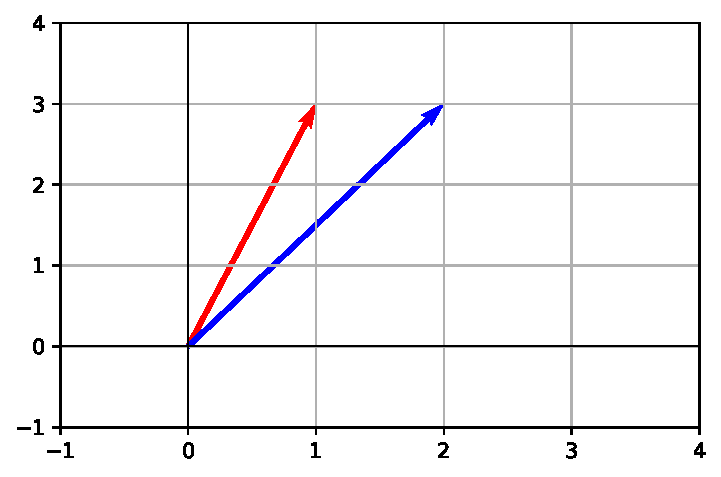
\includegraphics[keepaspectratio]{books/en-US/lab_files/figure-latex/cell-85-output-1.pdf}}

Red arrow = original vector, blue arrow = transformed vector.

\subsubsection{Try It Yourself}\label{try-it-yourself-112}

\begin{enumerate}
\def\labelenumi{\arabic{enumi}.}
\item
  Multiply

  \[
  A = \begin{bmatrix}1 & 0 \\ 0 & 1 \\ -1 & 2\end{bmatrix},\; x = [3,1]
  \]

  What's the result?
\item
  Replace \texttt{B} with \texttt{{[}{[}0,-1{]},{[}1,0{]}{]}}. Multiply
  it by \texttt{(1,0)} and \texttt{(0,1)}. What geometric transformation
  does this represent?
\item
  For a 4×4 identity matrix (\texttt{np.eye(4)}), try multiplying by any
  4D vector. What do you observe?
\end{enumerate}

\subsection{15. Matrix--Matrix Product (Composition of Linear
Steps)}\label{matrixmatrix-product-composition-of-linear-steps-1}

Matrix--matrix multiplication is how we combine two linear
transformations into one. Instead of applying one transformation, then
another, we can multiply their matrices and get a single matrix that
does both at once.

\subsubsection{Set Up Your Lab}\label{set-up-your-lab-14}

\begin{Shaded}
\begin{Highlighting}[]
\ImportTok{import}\NormalTok{ numpy }\ImportTok{as}\NormalTok{ np}
\end{Highlighting}
\end{Shaded}

\subsubsection{Step-by-Step Code
Walkthrough}\label{step-by-step-code-walkthrough-14}

\begin{enumerate}
\def\labelenumi{\arabic{enumi}.}
\tightlist
\item
  Matrix--matrix multiplication in NumPy
\end{enumerate}

\begin{Shaded}
\begin{Highlighting}[]
\NormalTok{A }\OperatorTok{=}\NormalTok{ np.array([}
\NormalTok{    [}\DecValTok{1}\NormalTok{, }\DecValTok{2}\NormalTok{],}
\NormalTok{    [}\DecValTok{3}\NormalTok{, }\DecValTok{4}\NormalTok{]}
\NormalTok{])  }\CommentTok{\# 2×2}

\NormalTok{B }\OperatorTok{=}\NormalTok{ np.array([}
\NormalTok{    [}\DecValTok{2}\NormalTok{, }\DecValTok{0}\NormalTok{],}
\NormalTok{    [}\DecValTok{1}\NormalTok{, }\DecValTok{2}\NormalTok{]}
\NormalTok{])  }\CommentTok{\# 2×2}

\NormalTok{C }\OperatorTok{=}\NormalTok{ A.dot(B)   }\CommentTok{\# or A @ B}
\BuiltInTok{print}\NormalTok{(}\StringTok{"A·B =}\CharTok{\textbackslash{}n}\StringTok{"}\NormalTok{, C)}
\end{Highlighting}
\end{Shaded}

\begin{verbatim}
A·B =
 [[ 4  4]
 [10  8]]
\end{verbatim}

The result \texttt{C} is another 2×2 matrix.

\begin{enumerate}
\def\labelenumi{\arabic{enumi}.}
\setcounter{enumi}{1}
\tightlist
\item
  Manual computation
\end{enumerate}

Each entry of \texttt{C} is computed as a row of A dotted with a column
of B:

\begin{Shaded}
\begin{Highlighting}[]
\NormalTok{c11 }\OperatorTok{=}\NormalTok{ A[}\DecValTok{0}\NormalTok{,:].dot(B[:,}\DecValTok{0}\NormalTok{])}
\NormalTok{c12 }\OperatorTok{=}\NormalTok{ A[}\DecValTok{0}\NormalTok{,:].dot(B[:,}\DecValTok{1}\NormalTok{])}
\NormalTok{c21 }\OperatorTok{=}\NormalTok{ A[}\DecValTok{1}\NormalTok{,:].dot(B[:,}\DecValTok{0}\NormalTok{])}
\NormalTok{c22 }\OperatorTok{=}\NormalTok{ A[}\DecValTok{1}\NormalTok{,:].dot(B[:,}\DecValTok{1}\NormalTok{])}

\BuiltInTok{print}\NormalTok{(}\StringTok{"Manual C =}\CharTok{\textbackslash{}n}\StringTok{"}\NormalTok{, np.array([[c11,c12],[c21,c22]]))}
\end{Highlighting}
\end{Shaded}

\begin{verbatim}
Manual C =
 [[ 4  4]
 [10  8]]
\end{verbatim}

This should match \texttt{A·B}.

\begin{enumerate}
\def\labelenumi{\arabic{enumi}.}
\setcounter{enumi}{2}
\tightlist
\item
  Geometric interpretation
\end{enumerate}

Let's see how two transformations combine.

\begin{itemize}
\tightlist
\item
  Matrix \texttt{B} scales x by 2 and stretches y by 2.
\item
  Matrix \texttt{A} applies another linear transformation.
\end{itemize}

Together, \texttt{C\ =\ A·B} does both in one step.

\begin{Shaded}
\begin{Highlighting}[]
\NormalTok{v }\OperatorTok{=}\NormalTok{ np.array([}\DecValTok{1}\NormalTok{,}\DecValTok{1}\NormalTok{])}

\BuiltInTok{print}\NormalTok{(}\StringTok{"First apply B:"}\NormalTok{, B.dot(v))}
\BuiltInTok{print}\NormalTok{(}\StringTok{"Then apply A:"}\NormalTok{, A.dot(B.dot(v)))}
\BuiltInTok{print}\NormalTok{(}\StringTok{"Directly with C:"}\NormalTok{, C.dot(v))}
\end{Highlighting}
\end{Shaded}

\begin{verbatim}
First apply B: [2 3]
Then apply A: [ 8 18]
Directly with C: [ 8 18]
\end{verbatim}

The result is the same: applying \texttt{B} then \texttt{A} is
equivalent to applying \texttt{C}.

\begin{enumerate}
\def\labelenumi{\arabic{enumi}.}
\setcounter{enumi}{3}
\tightlist
\item
  Non-square matrices
\end{enumerate}

Matrix multiplication also works for rectangular matrices, as long as
the inner dimensions match.

\begin{Shaded}
\begin{Highlighting}[]
\NormalTok{M }\OperatorTok{=}\NormalTok{ np.array([}
\NormalTok{    [}\DecValTok{1}\NormalTok{, }\DecValTok{0}\NormalTok{, }\DecValTok{2}\NormalTok{],}
\NormalTok{    [}\DecValTok{0}\NormalTok{, }\DecValTok{1}\NormalTok{, }\DecValTok{3}\NormalTok{]}
\NormalTok{])  }\CommentTok{\# 2×3}

\NormalTok{N }\OperatorTok{=}\NormalTok{ np.array([}
\NormalTok{    [}\DecValTok{1}\NormalTok{, }\DecValTok{2}\NormalTok{],}
\NormalTok{    [}\DecValTok{0}\NormalTok{, }\DecValTok{1}\NormalTok{],}
\NormalTok{    [}\DecValTok{4}\NormalTok{, }\DecValTok{0}\NormalTok{]}
\NormalTok{])  }\CommentTok{\# 3×2}

\NormalTok{P }\OperatorTok{=}\NormalTok{ M.dot(N)  }\CommentTok{\# result is 2×2}
\BuiltInTok{print}\NormalTok{(}\StringTok{"M·N =}\CharTok{\textbackslash{}n}\StringTok{"}\NormalTok{, P)}
\end{Highlighting}
\end{Shaded}

\begin{verbatim}
M·N =
 [[ 9  2]
 [12  1]]
\end{verbatim}

Shape rule: \texttt{(2×3)·(3×2)\ =\ (2×2)}.

\begin{enumerate}
\def\labelenumi{\arabic{enumi}.}
\setcounter{enumi}{4}
\tightlist
\item
  Associativity (but not commutativity)
\end{enumerate}

Matrix multiplication is associative: \texttt{(A·B)·C\ =\ A·(B·C)}. But
it's not commutative: in general, \texttt{A·B\ ≠\ B·A}.

\begin{Shaded}
\begin{Highlighting}[]
\NormalTok{A }\OperatorTok{=}\NormalTok{ np.array([[}\DecValTok{1}\NormalTok{,}\DecValTok{2}\NormalTok{],[}\DecValTok{3}\NormalTok{,}\DecValTok{4}\NormalTok{]])}
\NormalTok{B }\OperatorTok{=}\NormalTok{ np.array([[}\DecValTok{0}\NormalTok{,}\DecValTok{1}\NormalTok{],[}\DecValTok{1}\NormalTok{,}\DecValTok{0}\NormalTok{]])}

\BuiltInTok{print}\NormalTok{(}\StringTok{"A·B =}\CharTok{\textbackslash{}n}\StringTok{"}\NormalTok{, A.dot(B))}
\BuiltInTok{print}\NormalTok{(}\StringTok{"B·A =}\CharTok{\textbackslash{}n}\StringTok{"}\NormalTok{, B.dot(A))}
\end{Highlighting}
\end{Shaded}

\begin{verbatim}
A·B =
 [[2 1]
 [4 3]]
B·A =
 [[3 4]
 [1 2]]
\end{verbatim}

The two results are different.

\subsubsection{Try It Yourself}\label{try-it-yourself-113}

\begin{enumerate}
\def\labelenumi{\arabic{enumi}.}
\item
  Multiply

  \[
  A = \begin{bmatrix}1 & 0 \\ 0 & 1\end{bmatrix},\; 
  B = \begin{bmatrix}0 & -1 \\ 1 & 0\end{bmatrix}
  \]

  What transformation does \texttt{A·B} represent?
\item
  Create a random 3×2 matrix and a 2×4 matrix. Multiply them. What shape
  is the result?
\item
  Verify with Python that \texttt{(A·B)·C\ =\ A·(B·C)} for some 3×3
  random matrices.
\end{enumerate}

\subsection{16. Identity, Inverse, and
Transpose}\label{identity-inverse-and-transpose-1}

In this lab, we'll meet three special matrix operations and objects: the
identity matrix, the inverse, and the transpose. These are the building
blocks of matrix algebra, each with a simple meaning but deep
importance.

\subsubsection{Set Up Your Lab}\label{set-up-your-lab-15}

\begin{Shaded}
\begin{Highlighting}[]
\ImportTok{import}\NormalTok{ numpy }\ImportTok{as}\NormalTok{ np}
\end{Highlighting}
\end{Shaded}

\subsubsection{Step-by-Step Code
Walkthrough}\label{step-by-step-code-walkthrough-15}

\begin{enumerate}
\def\labelenumi{\arabic{enumi}.}
\tightlist
\item
  Identity matrix The identity matrix is like the number \texttt{1} for
  matrices: multiplying by it changes nothing.
\end{enumerate}

\begin{Shaded}
\begin{Highlighting}[]
\NormalTok{I }\OperatorTok{=}\NormalTok{ np.eye(}\DecValTok{3}\NormalTok{)  }\CommentTok{\# 3×3 identity matrix}
\BuiltInTok{print}\NormalTok{(}\StringTok{"Identity matrix:}\CharTok{\textbackslash{}n}\StringTok{"}\NormalTok{, I)}

\NormalTok{A }\OperatorTok{=}\NormalTok{ np.array([}
\NormalTok{    [}\DecValTok{2}\NormalTok{, }\DecValTok{1}\NormalTok{, }\DecValTok{0}\NormalTok{],}
\NormalTok{    [}\DecValTok{0}\NormalTok{, }\DecValTok{1}\NormalTok{, }\DecValTok{3}\NormalTok{],}
\NormalTok{    [}\DecValTok{4}\NormalTok{, }\DecValTok{0}\NormalTok{, }\DecValTok{1}\NormalTok{]}
\NormalTok{])}

\BuiltInTok{print}\NormalTok{(}\StringTok{"A·I =}\CharTok{\textbackslash{}n}\StringTok{"}\NormalTok{, A.dot(I))}
\BuiltInTok{print}\NormalTok{(}\StringTok{"I·A =}\CharTok{\textbackslash{}n}\StringTok{"}\NormalTok{, I.dot(A))}
\end{Highlighting}
\end{Shaded}

\begin{verbatim}
Identity matrix:
 [[1. 0. 0.]
 [0. 1. 0.]
 [0. 0. 1.]]
A·I =
 [[2. 1. 0.]
 [0. 1. 3.]
 [4. 0. 1.]]
I·A =
 [[2. 1. 0.]
 [0. 1. 3.]
 [4. 0. 1.]]
\end{verbatim}

Both equal \texttt{A}.

\begin{enumerate}
\def\labelenumi{\arabic{enumi}.}
\setcounter{enumi}{1}
\tightlist
\item
  Transpose The transpose flips rows and columns.
\end{enumerate}

\begin{Shaded}
\begin{Highlighting}[]
\NormalTok{B }\OperatorTok{=}\NormalTok{ np.array([}
\NormalTok{    [}\DecValTok{1}\NormalTok{, }\DecValTok{2}\NormalTok{, }\DecValTok{3}\NormalTok{],}
\NormalTok{    [}\DecValTok{4}\NormalTok{, }\DecValTok{5}\NormalTok{, }\DecValTok{6}\NormalTok{]}
\NormalTok{])}

\BuiltInTok{print}\NormalTok{(}\StringTok{"B:}\CharTok{\textbackslash{}n}\StringTok{"}\NormalTok{, B)}
\BuiltInTok{print}\NormalTok{(}\StringTok{"B.T:}\CharTok{\textbackslash{}n}\StringTok{"}\NormalTok{, B.T)}
\end{Highlighting}
\end{Shaded}

\begin{verbatim}
B:
 [[1 2 3]
 [4 5 6]]
B.T:
 [[1 4]
 [2 5]
 [3 6]]
\end{verbatim}

\begin{itemize}
\tightlist
\item
  Original: 2×3
\item
  Transpose: 3×2
\end{itemize}

Geometrically, transpose swaps the axes when vectors are viewed in
row/column form.

\begin{enumerate}
\def\labelenumi{\arabic{enumi}.}
\setcounter{enumi}{2}
\tightlist
\item
  Inverse The inverse matrix is like dividing by a number: multiplying a
  matrix by its inverse gives the identity.
\end{enumerate}

\begin{Shaded}
\begin{Highlighting}[]
\NormalTok{C }\OperatorTok{=}\NormalTok{ np.array([}
\NormalTok{    [}\DecValTok{2}\NormalTok{, }\DecValTok{1}\NormalTok{],}
\NormalTok{    [}\DecValTok{5}\NormalTok{, }\DecValTok{3}\NormalTok{]}
\NormalTok{])}

\NormalTok{C\_inv }\OperatorTok{=}\NormalTok{ np.linalg.inv(C)}
\BuiltInTok{print}\NormalTok{(}\StringTok{"Inverse of C:}\CharTok{\textbackslash{}n}\StringTok{"}\NormalTok{, C\_inv)}

\BuiltInTok{print}\NormalTok{(}\StringTok{"C·C\_inv =}\CharTok{\textbackslash{}n}\StringTok{"}\NormalTok{, C.dot(C\_inv))}
\BuiltInTok{print}\NormalTok{(}\StringTok{"C\_inv·C =}\CharTok{\textbackslash{}n}\StringTok{"}\NormalTok{, C\_inv.dot(C))}
\end{Highlighting}
\end{Shaded}

\begin{verbatim}
Inverse of C:
 [[ 3. -1.]
 [-5.  2.]]
C·C_inv =
 [[ 1.00000000e+00  2.22044605e-16]
 [-8.88178420e-16  1.00000000e+00]]
C_inv·C =
 [[1.00000000e+00 3.33066907e-16]
 [0.00000000e+00 1.00000000e+00]]
\end{verbatim}

Both products are (approximately) the identity.

\begin{enumerate}
\def\labelenumi{\arabic{enumi}.}
\setcounter{enumi}{3}
\tightlist
\item
  Matrices that don't have inverses Not every matrix is invertible. If a
  matrix is singular (determinant = 0), it has no inverse.
\end{enumerate}

\begin{Shaded}
\begin{Highlighting}[]
\NormalTok{D }\OperatorTok{=}\NormalTok{ np.array([}
\NormalTok{    [}\DecValTok{1}\NormalTok{, }\DecValTok{2}\NormalTok{],}
\NormalTok{    [}\DecValTok{2}\NormalTok{, }\DecValTok{4}\NormalTok{]}
\NormalTok{])}

\ControlFlowTok{try}\NormalTok{:}
\NormalTok{    np.linalg.inv(D)}
\ControlFlowTok{except}\NormalTok{ np.linalg.LinAlgError }\ImportTok{as}\NormalTok{ e:}
    \BuiltInTok{print}\NormalTok{(}\StringTok{"Error:"}\NormalTok{, e)}
\end{Highlighting}
\end{Shaded}

\begin{verbatim}
Error: Singular matrix
\end{verbatim}

Here, the second row is a multiple of the first, so \texttt{D} can't be
inverted.

\begin{enumerate}
\def\labelenumi{\arabic{enumi}.}
\setcounter{enumi}{4}
\tightlist
\item
  Transpose and inverse together For invertible matrices,
\end{enumerate}

\[
(A^T)^{-1} = (A^{-1})^T
\]

We can check this numerically:

\begin{Shaded}
\begin{Highlighting}[]
\NormalTok{A }\OperatorTok{=}\NormalTok{ np.array([}
\NormalTok{    [}\DecValTok{1}\NormalTok{, }\DecValTok{2}\NormalTok{],}
\NormalTok{    [}\DecValTok{3}\NormalTok{, }\DecValTok{5}\NormalTok{]}
\NormalTok{])}

\NormalTok{lhs }\OperatorTok{=}\NormalTok{ np.linalg.inv(A.T)}
\NormalTok{rhs }\OperatorTok{=}\NormalTok{ np.linalg.inv(A).T}

\BuiltInTok{print}\NormalTok{(}\StringTok{"Do they match?"}\NormalTok{, np.allclose(lhs, rhs))}
\end{Highlighting}
\end{Shaded}

\begin{verbatim}
Do they match? True
\end{verbatim}

\subsubsection{Try It Yourself}\label{try-it-yourself-114}

\begin{enumerate}
\def\labelenumi{\arabic{enumi}.}
\tightlist
\item
  Create a 4×4 identity matrix. Multiply it by any 4×1 vector. Does it
  change?
\item
  Take a random 2×2 matrix with \texttt{np.random.randint}. Compute its
  inverse and check if multiplying gives identity.
\item
  Pick a rectangular 3×2 matrix. What happens when you try
  \texttt{np.linalg.inv}? Why?
\item
  Compute \texttt{(A.T).T} for some matrix \texttt{A}. What do you
  notice?
\end{enumerate}

\subsection{17. Symmetric, Diagonal, Triangular, and Permutation
Matrices}\label{symmetric-diagonal-triangular-and-permutation-matrices-1}

In this lab, we'll meet four important families of special matrices.
They have patterns that make them easier to understand, compute with,
and use in algorithms.

\subsubsection{Set Up Your Lab}\label{set-up-your-lab-16}

\begin{Shaded}
\begin{Highlighting}[]
\ImportTok{import}\NormalTok{ numpy }\ImportTok{as}\NormalTok{ np}
\end{Highlighting}
\end{Shaded}

\subsubsection{Step-by-Step Code
Walkthrough}\label{step-by-step-code-walkthrough-16}

\begin{enumerate}
\def\labelenumi{\arabic{enumi}.}
\tightlist
\item
  Symmetric matrices A matrix is symmetric if it equals its transpose:
  \(A = A^T\).
\end{enumerate}

\begin{Shaded}
\begin{Highlighting}[]
\NormalTok{A }\OperatorTok{=}\NormalTok{ np.array([}
\NormalTok{    [}\DecValTok{2}\NormalTok{, }\DecValTok{3}\NormalTok{, }\DecValTok{4}\NormalTok{],}
\NormalTok{    [}\DecValTok{3}\NormalTok{, }\DecValTok{5}\NormalTok{, }\DecValTok{6}\NormalTok{],}
\NormalTok{    [}\DecValTok{4}\NormalTok{, }\DecValTok{6}\NormalTok{, }\DecValTok{8}\NormalTok{]}
\NormalTok{])}

\BuiltInTok{print}\NormalTok{(}\StringTok{"A:}\CharTok{\textbackslash{}n}\StringTok{"}\NormalTok{, A)}
\BuiltInTok{print}\NormalTok{(}\StringTok{"A.T:}\CharTok{\textbackslash{}n}\StringTok{"}\NormalTok{, A.T)}
\BuiltInTok{print}\NormalTok{(}\StringTok{"Is symmetric?"}\NormalTok{, np.allclose(A, A.T))}
\end{Highlighting}
\end{Shaded}

\begin{verbatim}
A:
 [[2 3 4]
 [3 5 6]
 [4 6 8]]
A.T:
 [[2 3 4]
 [3 5 6]
 [4 6 8]]
Is symmetric? True
\end{verbatim}

Symmetric matrices appear in physics, optimization, and statistics
(e.g., covariance matrices).

\begin{enumerate}
\def\labelenumi{\arabic{enumi}.}
\setcounter{enumi}{1}
\tightlist
\item
  Diagonal matrices A diagonal matrix has nonzero entries only on the
  main diagonal.
\end{enumerate}

\begin{Shaded}
\begin{Highlighting}[]
\NormalTok{D }\OperatorTok{=}\NormalTok{ np.diag([}\DecValTok{1}\NormalTok{, }\DecValTok{5}\NormalTok{, }\DecValTok{9}\NormalTok{])}
\BuiltInTok{print}\NormalTok{(}\StringTok{"Diagonal matrix:}\CharTok{\textbackslash{}n}\StringTok{"}\NormalTok{, D)}

\NormalTok{x }\OperatorTok{=}\NormalTok{ np.array([}\DecValTok{2}\NormalTok{, }\DecValTok{3}\NormalTok{, }\DecValTok{4}\NormalTok{])}
\BuiltInTok{print}\NormalTok{(}\StringTok{"D·x ="}\NormalTok{, D.dot(x))  }\CommentTok{\# scales each component}
\end{Highlighting}
\end{Shaded}

\begin{verbatim}
Diagonal matrix:
 [[1 0 0]
 [0 5 0]
 [0 0 9]]
D·x = [ 2 15 36]
\end{verbatim}

Diagonal multiplication simply scales each coordinate separately.

\begin{enumerate}
\def\labelenumi{\arabic{enumi}.}
\setcounter{enumi}{2}
\tightlist
\item
  Triangular matrices Upper triangular: all entries below the diagonal
  are zero. Lower triangular: all entries above the diagonal are zero.
\end{enumerate}

\begin{Shaded}
\begin{Highlighting}[]
\NormalTok{U }\OperatorTok{=}\NormalTok{ np.array([}
\NormalTok{    [}\DecValTok{1}\NormalTok{, }\DecValTok{2}\NormalTok{, }\DecValTok{3}\NormalTok{],}
\NormalTok{    [}\DecValTok{0}\NormalTok{, }\DecValTok{4}\NormalTok{, }\DecValTok{5}\NormalTok{],}
\NormalTok{    [}\DecValTok{0}\NormalTok{, }\DecValTok{0}\NormalTok{, }\DecValTok{6}\NormalTok{]}
\NormalTok{])}

\NormalTok{L }\OperatorTok{=}\NormalTok{ np.array([}
\NormalTok{    [}\DecValTok{7}\NormalTok{, }\DecValTok{0}\NormalTok{, }\DecValTok{0}\NormalTok{],}
\NormalTok{    [}\DecValTok{8}\NormalTok{, }\DecValTok{9}\NormalTok{, }\DecValTok{0}\NormalTok{],}
\NormalTok{    [}\DecValTok{1}\NormalTok{, }\DecValTok{2}\NormalTok{, }\DecValTok{3}\NormalTok{]}
\NormalTok{])}

\BuiltInTok{print}\NormalTok{(}\StringTok{"Upper triangular U:}\CharTok{\textbackslash{}n}\StringTok{"}\NormalTok{, U)}
\BuiltInTok{print}\NormalTok{(}\StringTok{"Lower triangular L:}\CharTok{\textbackslash{}n}\StringTok{"}\NormalTok{, L)}
\end{Highlighting}
\end{Shaded}

\begin{verbatim}
Upper triangular U:
 [[1 2 3]
 [0 4 5]
 [0 0 6]]
Lower triangular L:
 [[7 0 0]
 [8 9 0]
 [1 2 3]]
\end{verbatim}

These are important in solving linear systems (e.g., Gaussian
elimination).

\begin{enumerate}
\def\labelenumi{\arabic{enumi}.}
\setcounter{enumi}{3}
\tightlist
\item
  Permutation matrices A permutation matrix rearranges the order of
  coordinates. Each row and each column has exactly one \texttt{1},
  everything else is \texttt{0}.
\end{enumerate}

\begin{Shaded}
\begin{Highlighting}[]
\NormalTok{P }\OperatorTok{=}\NormalTok{ np.array([}
\NormalTok{    [}\DecValTok{0}\NormalTok{, }\DecValTok{1}\NormalTok{, }\DecValTok{0}\NormalTok{],}
\NormalTok{    [}\DecValTok{0}\NormalTok{, }\DecValTok{0}\NormalTok{, }\DecValTok{1}\NormalTok{],}
\NormalTok{    [}\DecValTok{1}\NormalTok{, }\DecValTok{0}\NormalTok{, }\DecValTok{0}\NormalTok{]}
\NormalTok{])}

\BuiltInTok{print}\NormalTok{(}\StringTok{"Permutation matrix P:}\CharTok{\textbackslash{}n}\StringTok{"}\NormalTok{, P)}

\NormalTok{v }\OperatorTok{=}\NormalTok{ np.array([}\DecValTok{10}\NormalTok{, }\DecValTok{20}\NormalTok{, }\DecValTok{30}\NormalTok{])}
\BuiltInTok{print}\NormalTok{(}\StringTok{"P·v ="}\NormalTok{, P.dot(v))}
\end{Highlighting}
\end{Shaded}

\begin{verbatim}
Permutation matrix P:
 [[0 1 0]
 [0 0 1]
 [1 0 0]]
P·v = [20 30 10]
\end{verbatim}

Here, \texttt{P} cycles \texttt{(10,20,30)} into \texttt{(20,30,10)}.

\begin{enumerate}
\def\labelenumi{\arabic{enumi}.}
\setcounter{enumi}{4}
\tightlist
\item
  Checking properties
\end{enumerate}

\begin{Shaded}
\begin{Highlighting}[]
\KeywordTok{def}\NormalTok{ is\_symmetric(M): }\ControlFlowTok{return}\NormalTok{ np.allclose(M, M.T)}
\KeywordTok{def}\NormalTok{ is\_diagonal(M): }\ControlFlowTok{return}\NormalTok{ np.count\_nonzero(M }\OperatorTok{{-}}\NormalTok{ np.diag(np.diag(M))) }\OperatorTok{==} \DecValTok{0}
\KeywordTok{def}\NormalTok{ is\_upper\_triangular(M): }\ControlFlowTok{return}\NormalTok{ np.allclose(M, np.triu(M))}
\KeywordTok{def}\NormalTok{ is\_lower\_triangular(M): }\ControlFlowTok{return}\NormalTok{ np.allclose(M, np.tril(M))}

\BuiltInTok{print}\NormalTok{(}\StringTok{"A symmetric?"}\NormalTok{, is\_symmetric(A))}
\BuiltInTok{print}\NormalTok{(}\StringTok{"D diagonal?"}\NormalTok{, is\_diagonal(D))}
\BuiltInTok{print}\NormalTok{(}\StringTok{"U upper triangular?"}\NormalTok{, is\_upper\_triangular(U))}
\BuiltInTok{print}\NormalTok{(}\StringTok{"L lower triangular?"}\NormalTok{, is\_lower\_triangular(L))}
\end{Highlighting}
\end{Shaded}

\begin{verbatim}
A symmetric? True
D diagonal? True
U upper triangular? True
L lower triangular? True
\end{verbatim}

\subsubsection{Try It Yourself}\label{try-it-yourself-115}

\begin{enumerate}
\def\labelenumi{\arabic{enumi}.}
\tightlist
\item
  Create a random symmetric matrix by generating any matrix \texttt{M}
  and computing \texttt{(M\ +\ M.T)/2}.
\item
  Build a 4×4 diagonal matrix with diagonal entries
  \texttt{{[}2,4,6,8{]}} and multiply it by \texttt{{[}1,1,1,1{]}}.
\item
  Make a permutation matrix that swaps the first and last components of
  a 3D vector.
\item
  Check whether the identity matrix is diagonal, symmetric, upper
  triangular, and lower triangular all at once.
\end{enumerate}

\subsection{18. Trace and Basic Matrix
Properties}\label{trace-and-basic-matrix-properties-1}

In this lab, we'll introduce the trace of a matrix and a few quick
properties that often appear in proofs, algorithms, and applications.
The trace is simple to compute but surprisingly powerful.

\subsubsection{Set Up Your Lab}\label{set-up-your-lab-17}

\begin{Shaded}
\begin{Highlighting}[]
\ImportTok{import}\NormalTok{ numpy }\ImportTok{as}\NormalTok{ np}
\end{Highlighting}
\end{Shaded}

\subsubsection{Step-by-Step Code
Walkthrough}\label{step-by-step-code-walkthrough-17}

\begin{enumerate}
\def\labelenumi{\arabic{enumi}.}
\tightlist
\item
  What is the trace? The trace of a square matrix is the sum of its
  diagonal entries:
\end{enumerate}

\[
\text{tr}(A) = \sum_i A_{ii}
\]

\begin{Shaded}
\begin{Highlighting}[]
\NormalTok{A }\OperatorTok{=}\NormalTok{ np.array([}
\NormalTok{    [}\DecValTok{2}\NormalTok{, }\DecValTok{1}\NormalTok{, }\DecValTok{3}\NormalTok{],}
\NormalTok{    [}\DecValTok{0}\NormalTok{, }\DecValTok{4}\NormalTok{, }\DecValTok{5}\NormalTok{],}
\NormalTok{    [}\DecValTok{7}\NormalTok{, }\DecValTok{8}\NormalTok{, }\DecValTok{6}\NormalTok{]}
\NormalTok{])}

\NormalTok{trace\_A }\OperatorTok{=}\NormalTok{ np.trace(A)}
\BuiltInTok{print}\NormalTok{(}\StringTok{"Matrix A:}\CharTok{\textbackslash{}n}\StringTok{"}\NormalTok{, A)}
\BuiltInTok{print}\NormalTok{(}\StringTok{"Trace of A ="}\NormalTok{, trace\_A)}
\end{Highlighting}
\end{Shaded}

\begin{verbatim}
Matrix A:
 [[2 1 3]
 [0 4 5]
 [7 8 6]]
Trace of A = 12
\end{verbatim}

Here, trace = \(2 + 4 + 6 = 12\).

\begin{enumerate}
\def\labelenumi{\arabic{enumi}.}
\setcounter{enumi}{1}
\tightlist
\item
  Trace is linear For matrices \texttt{A} and \texttt{B}:
\end{enumerate}

\[
\text{tr}(A+B) = \text{tr}(A) + \text{tr}(B)
\]

\[
\text{tr}(cA) = c \cdot \text{tr}(A)
\]

\begin{Shaded}
\begin{Highlighting}[]
\NormalTok{B }\OperatorTok{=}\NormalTok{ np.array([}
\NormalTok{    [}\DecValTok{1}\NormalTok{, }\DecValTok{0}\NormalTok{, }\DecValTok{0}\NormalTok{],}
\NormalTok{    [}\DecValTok{0}\NormalTok{, }\DecValTok{2}\NormalTok{, }\DecValTok{0}\NormalTok{],}
\NormalTok{    [}\DecValTok{0}\NormalTok{, }\DecValTok{0}\NormalTok{, }\DecValTok{3}\NormalTok{]}
\NormalTok{])}

\BuiltInTok{print}\NormalTok{(}\StringTok{"tr(A+B) ="}\NormalTok{, np.trace(A}\OperatorTok{+}\NormalTok{B))}
\BuiltInTok{print}\NormalTok{(}\StringTok{"tr(A) + tr(B) ="}\NormalTok{, np.trace(A) }\OperatorTok{+}\NormalTok{ np.trace(B))}

\BuiltInTok{print}\NormalTok{(}\StringTok{"tr(3A) ="}\NormalTok{, np.trace(}\DecValTok{3}\OperatorTok{*}\NormalTok{A))}
\BuiltInTok{print}\NormalTok{(}\StringTok{"3 * tr(A) ="}\NormalTok{, }\DecValTok{3}\OperatorTok{*}\NormalTok{np.trace(A))}
\end{Highlighting}
\end{Shaded}

\begin{verbatim}
tr(A+B) = 18
tr(A) + tr(B) = 18
tr(3A) = 36
3 * tr(A) = 36
\end{verbatim}

\begin{enumerate}
\def\labelenumi{\arabic{enumi}.}
\setcounter{enumi}{2}
\tightlist
\item
  Trace of a product One important property is:
\end{enumerate}

\[
\text{tr}(AB) = \text{tr}(BA)
\]

\begin{Shaded}
\begin{Highlighting}[]
\NormalTok{C }\OperatorTok{=}\NormalTok{ np.array([}
\NormalTok{    [}\DecValTok{0}\NormalTok{,}\DecValTok{1}\NormalTok{],}
\NormalTok{    [}\DecValTok{2}\NormalTok{,}\DecValTok{3}\NormalTok{]}
\NormalTok{])}

\NormalTok{D }\OperatorTok{=}\NormalTok{ np.array([}
\NormalTok{    [}\DecValTok{4}\NormalTok{,}\DecValTok{5}\NormalTok{],}
\NormalTok{    [}\DecValTok{6}\NormalTok{,}\DecValTok{7}\NormalTok{]}
\NormalTok{])}

\BuiltInTok{print}\NormalTok{(}\StringTok{"tr(CD) ="}\NormalTok{, np.trace(C.dot(D)))}
\BuiltInTok{print}\NormalTok{(}\StringTok{"tr(DC) ="}\NormalTok{, np.trace(D.dot(C)))}
\end{Highlighting}
\end{Shaded}

\begin{verbatim}
tr(CD) = 37
tr(DC) = 37
\end{verbatim}

Both are equal, even though \texttt{CD} and \texttt{DC} are different
matrices.

\begin{enumerate}
\def\labelenumi{\arabic{enumi}.}
\setcounter{enumi}{3}
\tightlist
\item
  Trace and eigenvalues The trace equals the sum of eigenvalues of a
  matrix (counting multiplicities).
\end{enumerate}

\begin{Shaded}
\begin{Highlighting}[]
\NormalTok{vals, vecs }\OperatorTok{=}\NormalTok{ np.linalg.eig(A)}
\BuiltInTok{print}\NormalTok{(}\StringTok{"Eigenvalues:"}\NormalTok{, vals)}
\BuiltInTok{print}\NormalTok{(}\StringTok{"Sum of eigenvalues ="}\NormalTok{, np.}\BuiltInTok{sum}\NormalTok{(vals))}
\BuiltInTok{print}\NormalTok{(}\StringTok{"Trace ="}\NormalTok{, np.trace(A))}
\end{Highlighting}
\end{Shaded}

\begin{verbatim}
Eigenvalues: [12.83286783  2.13019807 -2.9630659 ]
Sum of eigenvalues = 12.000000000000007
Trace = 12
\end{verbatim}

The results should match (within rounding error).

\begin{enumerate}
\def\labelenumi{\arabic{enumi}.}
\setcounter{enumi}{4}
\tightlist
\item
  Quick invariants
\end{enumerate}

\begin{itemize}
\tightlist
\item
  Trace doesn't change under transpose: \texttt{tr(A)\ =\ tr(A.T)}
\item
  Trace doesn't change under similarity transforms:
  \texttt{tr(P\^{}-1\ A\ P)\ =\ tr(A)}
\end{itemize}

\begin{Shaded}
\begin{Highlighting}[]
\BuiltInTok{print}\NormalTok{(}\StringTok{"tr(A) ="}\NormalTok{, np.trace(A))}
\BuiltInTok{print}\NormalTok{(}\StringTok{"tr(A.T) ="}\NormalTok{, np.trace(A.T))}
\end{Highlighting}
\end{Shaded}

\begin{verbatim}
tr(A) = 12
tr(A.T) = 12
\end{verbatim}

\subsubsection{Try It Yourself}\label{try-it-yourself-116}

\begin{enumerate}
\def\labelenumi{\arabic{enumi}.}
\item
  Create a 2×2 rotation matrix for 90°:

  \[
  R = \begin{bmatrix}0 & -1 \\ 1 & 0\end{bmatrix}
  \]

  What is its trace? What does that tell you about its eigenvalues?
\item
  Make a random 3×3 matrix and compare \texttt{tr(A)} with the sum of
  eigenvalues.
\item
  Test \texttt{tr(AB)} and \texttt{tr(BA)} with a rectangular matrix
  \texttt{A} (e.g.~2×3) and \texttt{B} (3×2). Do they still match?
\end{enumerate}

\subsection{19. Affine Transforms and Homogeneous
Coordinates}\label{affine-transforms-and-homogeneous-coordinates-1}

Affine transformations let us do more than just linear operations - they
include translations (shifting points), which ordinary matrices can't
handle alone. To unify rotations, scalings, reflections, and
translations, we use homogeneous coordinates.

\subsubsection{Set Up Your Lab}\label{set-up-your-lab-18}

\begin{Shaded}
\begin{Highlighting}[]
\ImportTok{import}\NormalTok{ numpy }\ImportTok{as}\NormalTok{ np}
\ImportTok{import}\NormalTok{ matplotlib.pyplot }\ImportTok{as}\NormalTok{ plt}
\end{Highlighting}
\end{Shaded}

\subsubsection{Step-by-Step Code
Walkthrough}\label{step-by-step-code-walkthrough-18}

\begin{enumerate}
\def\labelenumi{\arabic{enumi}.}
\tightlist
\item
  Linear transformations vs affine transformations
\end{enumerate}

\begin{itemize}
\tightlist
\item
  A linear transformation can rotate, scale, or shear, but always keeps
  the origin fixed.
\item
  An affine transformation allows translation as well.
\end{itemize}

For example, shifting every point by \texttt{(2,3)} is affine but not
linear.

\begin{enumerate}
\def\labelenumi{\arabic{enumi}.}
\setcounter{enumi}{1}
\tightlist
\item
  Homogeneous coordinates idea We add an extra coordinate (usually
  \texttt{1}) to vectors.
\end{enumerate}

\begin{itemize}
\tightlist
\item
  A 2D point \texttt{(x,y)} becomes \texttt{(x,y,1)}.
\item
  A 3D point \texttt{(x,y,z)} becomes \texttt{(x,y,z,1)}.
\end{itemize}

This trick lets us represent translations using matrix multiplication.

\begin{enumerate}
\def\labelenumi{\arabic{enumi}.}
\setcounter{enumi}{2}
\tightlist
\item
  2D translation matrix
\end{enumerate}

\[
T = \begin{bmatrix}
1 & 0 & t_x \\
0 & 1 & t_y \\
0 & 0 & 1
\end{bmatrix}
\]

\begin{Shaded}
\begin{Highlighting}[]
\NormalTok{T }\OperatorTok{=}\NormalTok{ np.array([}
\NormalTok{    [}\DecValTok{1}\NormalTok{, }\DecValTok{0}\NormalTok{, }\DecValTok{2}\NormalTok{],}
\NormalTok{    [}\DecValTok{0}\NormalTok{, }\DecValTok{1}\NormalTok{, }\DecValTok{3}\NormalTok{],}
\NormalTok{    [}\DecValTok{0}\NormalTok{, }\DecValTok{0}\NormalTok{, }\DecValTok{1}\NormalTok{]}
\NormalTok{])}

\NormalTok{p }\OperatorTok{=}\NormalTok{ np.array([}\DecValTok{1}\NormalTok{, }\DecValTok{1}\NormalTok{, }\DecValTok{1}\NormalTok{])  }\CommentTok{\# point at (1,1)}
\NormalTok{p\_translated }\OperatorTok{=}\NormalTok{ T.dot(p)}

\BuiltInTok{print}\NormalTok{(}\StringTok{"Original point:"}\NormalTok{, p)}
\BuiltInTok{print}\NormalTok{(}\StringTok{"Translated point:"}\NormalTok{, p\_translated)}
\end{Highlighting}
\end{Shaded}

\begin{verbatim}
Original point: [1 1 1]
Translated point: [3 4 1]
\end{verbatim}

This shifts \texttt{(1,1)} to \texttt{(3,4)}.

\begin{enumerate}
\def\labelenumi{\arabic{enumi}.}
\setcounter{enumi}{3}
\tightlist
\item
  Combining rotation and translation
\end{enumerate}

A 90° rotation around the origin in 2D:

\begin{Shaded}
\begin{Highlighting}[]
\NormalTok{R }\OperatorTok{=}\NormalTok{ np.array([}
\NormalTok{    [}\DecValTok{0}\NormalTok{, }\OperatorTok{{-}}\DecValTok{1}\NormalTok{, }\DecValTok{0}\NormalTok{],}
\NormalTok{    [}\DecValTok{1}\NormalTok{,  }\DecValTok{0}\NormalTok{, }\DecValTok{0}\NormalTok{],}
\NormalTok{    [}\DecValTok{0}\NormalTok{,  }\DecValTok{0}\NormalTok{, }\DecValTok{1}\NormalTok{]}
\NormalTok{])}

\NormalTok{M }\OperatorTok{=}\NormalTok{ T.dot(R)  }\CommentTok{\# rotate then translate}
\BuiltInTok{print}\NormalTok{(}\StringTok{"Combined transform:}\CharTok{\textbackslash{}n}\StringTok{"}\NormalTok{, M)}

\NormalTok{p }\OperatorTok{=}\NormalTok{ np.array([}\DecValTok{1}\NormalTok{, }\DecValTok{0}\NormalTok{, }\DecValTok{1}\NormalTok{])}
\BuiltInTok{print}\NormalTok{(}\StringTok{"Rotated + translated point:"}\NormalTok{, M.dot(p))}
\end{Highlighting}
\end{Shaded}

\begin{verbatim}
Combined transform:
 [[ 0 -1  2]
 [ 1  0  3]
 [ 0  0  1]]
Rotated + translated point: [2 4 1]
\end{verbatim}

Now we can apply rotation and translation in one step.

\begin{enumerate}
\def\labelenumi{\arabic{enumi}.}
\setcounter{enumi}{4}
\tightlist
\item
  Visualization of translation
\end{enumerate}

\begin{Shaded}
\begin{Highlighting}[]
\NormalTok{points }\OperatorTok{=}\NormalTok{ np.array([}
\NormalTok{    [}\DecValTok{0}\NormalTok{,}\DecValTok{0}\NormalTok{,}\DecValTok{1}\NormalTok{],}
\NormalTok{    [}\DecValTok{1}\NormalTok{,}\DecValTok{0}\NormalTok{,}\DecValTok{1}\NormalTok{],}
\NormalTok{    [}\DecValTok{1}\NormalTok{,}\DecValTok{1}\NormalTok{,}\DecValTok{1}\NormalTok{],}
\NormalTok{    [}\DecValTok{0}\NormalTok{,}\DecValTok{1}\NormalTok{,}\DecValTok{1}\NormalTok{]}
\NormalTok{])  }\CommentTok{\# a unit square}

\NormalTok{transformed }\OperatorTok{=}\NormalTok{ points.dot(T.T)}

\NormalTok{plt.scatter(points[:,}\DecValTok{0}\NormalTok{], points[:,}\DecValTok{1}\NormalTok{], color}\OperatorTok{=}\StringTok{\textquotesingle{}r\textquotesingle{}}\NormalTok{, label}\OperatorTok{=}\StringTok{\textquotesingle{}original\textquotesingle{}}\NormalTok{)}
\NormalTok{plt.scatter(transformed[:,}\DecValTok{0}\NormalTok{], transformed[:,}\DecValTok{1}\NormalTok{], color}\OperatorTok{=}\StringTok{\textquotesingle{}b\textquotesingle{}}\NormalTok{, label}\OperatorTok{=}\StringTok{\textquotesingle{}translated\textquotesingle{}}\NormalTok{)}

\ControlFlowTok{for}\NormalTok{ i }\KeywordTok{in} \BuiltInTok{range}\NormalTok{(}\BuiltInTok{len}\NormalTok{(points)):}
\NormalTok{    plt.arrow(points[i,}\DecValTok{0}\NormalTok{], points[i,}\DecValTok{1}\NormalTok{],}
\NormalTok{              transformed[i,}\DecValTok{0}\NormalTok{]}\OperatorTok{{-}}\NormalTok{points[i,}\DecValTok{0}\NormalTok{],}
\NormalTok{              transformed[i,}\DecValTok{1}\NormalTok{]}\OperatorTok{{-}}\NormalTok{points[i,}\DecValTok{1}\NormalTok{],}
\NormalTok{              head\_width}\OperatorTok{=}\FloatTok{0.05}\NormalTok{, color}\OperatorTok{=}\StringTok{\textquotesingle{}gray\textquotesingle{}}\NormalTok{)}

\NormalTok{plt.legend()}
\NormalTok{plt.axis(}\StringTok{\textquotesingle{}equal\textquotesingle{}}\NormalTok{)}
\NormalTok{plt.grid()}
\NormalTok{plt.show()}
\end{Highlighting}
\end{Shaded}

\pandocbounded{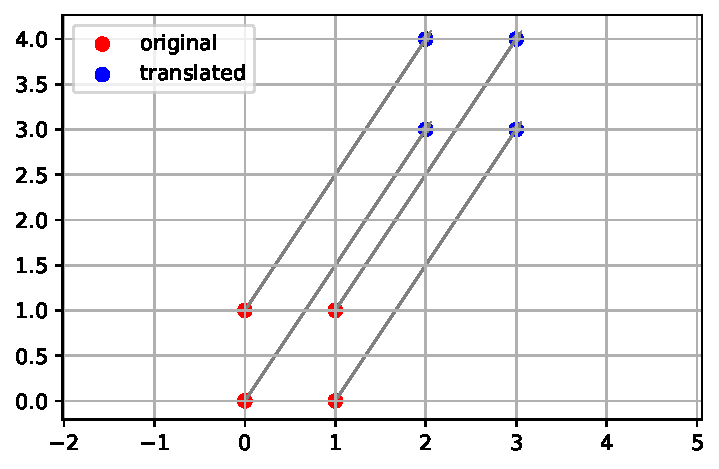
\includegraphics[keepaspectratio]{books/en-US/lab_files/figure-latex/cell-113-output-1.pdf}}

You'll see the red unit square moved to a blue unit square shifted by
\texttt{(2,3)}.

\begin{enumerate}
\def\labelenumi{\arabic{enumi}.}
\setcounter{enumi}{5}
\tightlist
\item
  Extending to 3D In 3D, homogeneous coordinates use 4×4 matrices.
  Translations, rotations, and scalings all fit the same framework.
\end{enumerate}

\begin{Shaded}
\begin{Highlighting}[]
\NormalTok{T3 }\OperatorTok{=}\NormalTok{ np.array([}
\NormalTok{    [}\DecValTok{1}\NormalTok{,}\DecValTok{0}\NormalTok{,}\DecValTok{0}\NormalTok{,}\DecValTok{5}\NormalTok{],}
\NormalTok{    [}\DecValTok{0}\NormalTok{,}\DecValTok{1}\NormalTok{,}\DecValTok{0}\NormalTok{,}\OperatorTok{{-}}\DecValTok{2}\NormalTok{],}
\NormalTok{    [}\DecValTok{0}\NormalTok{,}\DecValTok{0}\NormalTok{,}\DecValTok{1}\NormalTok{,}\DecValTok{3}\NormalTok{],}
\NormalTok{    [}\DecValTok{0}\NormalTok{,}\DecValTok{0}\NormalTok{,}\DecValTok{0}\NormalTok{,}\DecValTok{1}\NormalTok{]}
\NormalTok{])}

\NormalTok{p3 }\OperatorTok{=}\NormalTok{ np.array([}\DecValTok{1}\NormalTok{,}\DecValTok{2}\NormalTok{,}\DecValTok{3}\NormalTok{,}\DecValTok{1}\NormalTok{])}
\BuiltInTok{print}\NormalTok{(}\StringTok{"Translated 3D point:"}\NormalTok{, T3.dot(p3))}
\end{Highlighting}
\end{Shaded}

\begin{verbatim}
Translated 3D point: [6 0 6 1]
\end{verbatim}

This shifts \texttt{(1,2,3)} to \texttt{(6,0,6)}.

\subsubsection{Try It Yourself}\label{try-it-yourself-117}

\begin{enumerate}
\def\labelenumi{\arabic{enumi}.}
\tightlist
\item
  Build a scaling matrix in homogeneous coordinates that doubles both x
  and y, and apply it to \texttt{(1,1)}.
\item
  Create a 2D transform that rotates by 90° and then shifts by
  \texttt{(−2,1)}. Apply it to \texttt{(0,2)}.
\item
  In 3D, translate \texttt{(0,0,0)} by \texttt{(10,10,10)}. What
  homogeneous matrix did you use?
\end{enumerate}

\subsection{20. Computing with Matrices (Cost Counts and Simple
Speedups)}\label{computing-with-matrices-cost-counts-and-simple-speedups-1}

Working with matrices is not just about theory - in practice, we care
about how much computation it takes to perform operations, and how we
can make them faster. This lab introduces basic cost analysis (counting
operations) and demonstrates simple NumPy optimizations.

\subsubsection{Set Up Your Lab}\label{set-up-your-lab-19}

\begin{Shaded}
\begin{Highlighting}[]
\ImportTok{import}\NormalTok{ numpy }\ImportTok{as}\NormalTok{ np}
\ImportTok{import}\NormalTok{ time}
\end{Highlighting}
\end{Shaded}

\subsubsection{Step-by-Step Code
Walkthrough}\label{step-by-step-code-walkthrough-19}

\begin{enumerate}
\def\labelenumi{\arabic{enumi}.}
\tightlist
\item
  Counting operations (matrix--vector multiply)
\end{enumerate}

If \texttt{A} is an \(m \times n\) matrix and \texttt{x} is an
\(n\)-dimensional vector, computing \texttt{A·x} takes about
\(m \times n\) multiplications and the same number of additions.

\begin{Shaded}
\begin{Highlighting}[]
\NormalTok{m, n }\OperatorTok{=} \DecValTok{3}\NormalTok{, }\DecValTok{4}
\NormalTok{A }\OperatorTok{=}\NormalTok{ np.random.randint(}\DecValTok{1}\NormalTok{,}\DecValTok{10}\NormalTok{,(m,n))}
\NormalTok{x }\OperatorTok{=}\NormalTok{ np.random.randint(}\DecValTok{1}\NormalTok{,}\DecValTok{10}\NormalTok{,n)}

\BuiltInTok{print}\NormalTok{(}\StringTok{"Matrix A:}\CharTok{\textbackslash{}n}\StringTok{"}\NormalTok{, A)}
\BuiltInTok{print}\NormalTok{(}\StringTok{"Vector x:"}\NormalTok{, x)}
\BuiltInTok{print}\NormalTok{(}\StringTok{"A·x ="}\NormalTok{, A.dot(x))}
\end{Highlighting}
\end{Shaded}

\begin{verbatim}
Matrix A:
 [[6 6 6 2]
 [1 1 1 1]
 [1 8 7 4]]
Vector x: [6 5 4 5]
A·x = [100  20  94]
\end{verbatim}

Here the cost is \(3 \times 4 = 12\) multiplications + 12 additions.

\begin{enumerate}
\def\labelenumi{\arabic{enumi}.}
\setcounter{enumi}{1}
\tightlist
\item
  Counting operations (matrix--matrix multiply)
\end{enumerate}

For an \(m \times n\) times \(n \times p\) multiplication, the cost is
about \(m \times n \times p\).

\begin{Shaded}
\begin{Highlighting}[]
\NormalTok{m, n, p }\OperatorTok{=} \DecValTok{3}\NormalTok{, }\DecValTok{4}\NormalTok{, }\DecValTok{2}
\NormalTok{A }\OperatorTok{=}\NormalTok{ np.random.randint(}\DecValTok{1}\NormalTok{,}\DecValTok{10}\NormalTok{,(m,n))}
\NormalTok{B }\OperatorTok{=}\NormalTok{ np.random.randint(}\DecValTok{1}\NormalTok{,}\DecValTok{10}\NormalTok{,(n,p))}

\NormalTok{C }\OperatorTok{=}\NormalTok{ A.dot(B)}
\BuiltInTok{print}\NormalTok{(}\StringTok{"A·B =}\CharTok{\textbackslash{}n}\StringTok{"}\NormalTok{, C)}
\end{Highlighting}
\end{Shaded}

\begin{verbatim}
A·B =
 [[ 59  92]
 [ 43  81]
 [ 65 102]]
\end{verbatim}

Here the cost is \(3 \times 4 \times 2 = 24\) multiplications + 24
additions.

\begin{enumerate}
\def\labelenumi{\arabic{enumi}.}
\setcounter{enumi}{2}
\tightlist
\item
  Timing with NumPy (vectorized vs loop)
\end{enumerate}

NumPy is optimized in C and Fortran under the hood. Let's compare matrix
multiplication with and without vectorization.

\begin{Shaded}
\begin{Highlighting}[]
\NormalTok{n }\OperatorTok{=} \DecValTok{50}
\NormalTok{A }\OperatorTok{=}\NormalTok{ np.random.randn(n,n)}
\NormalTok{B }\OperatorTok{=}\NormalTok{ np.random.randn(n,n)}

\CommentTok{\# Vectorized}
\NormalTok{start }\OperatorTok{=}\NormalTok{ time.time()}
\NormalTok{C1 }\OperatorTok{=}\NormalTok{ A.dot(B)}
\NormalTok{end }\OperatorTok{=}\NormalTok{ time.time()}
\BuiltInTok{print}\NormalTok{(}\StringTok{"Vectorized dot:"}\NormalTok{, }\BuiltInTok{round}\NormalTok{(end}\OperatorTok{{-}}\NormalTok{start,}\DecValTok{3}\NormalTok{), }\StringTok{"seconds"}\NormalTok{)}

\CommentTok{\# Manual loops}
\NormalTok{C2 }\OperatorTok{=}\NormalTok{ np.zeros((n,n))}
\NormalTok{start }\OperatorTok{=}\NormalTok{ time.time()}
\ControlFlowTok{for}\NormalTok{ i }\KeywordTok{in} \BuiltInTok{range}\NormalTok{(n):}
    \ControlFlowTok{for}\NormalTok{ j }\KeywordTok{in} \BuiltInTok{range}\NormalTok{(n):}
        \ControlFlowTok{for}\NormalTok{ k }\KeywordTok{in} \BuiltInTok{range}\NormalTok{(n):}
\NormalTok{            C2[i,j] }\OperatorTok{+=}\NormalTok{ A[i,k]}\OperatorTok{*}\NormalTok{B[k,j]}
\NormalTok{end }\OperatorTok{=}\NormalTok{ time.time()}
\BuiltInTok{print}\NormalTok{(}\StringTok{"Triple loop:"}\NormalTok{, }\BuiltInTok{round}\NormalTok{(end}\OperatorTok{{-}}\NormalTok{start,}\DecValTok{3}\NormalTok{), }\StringTok{"seconds"}\NormalTok{)}
\end{Highlighting}
\end{Shaded}

\begin{verbatim}
Vectorized dot: 0.0 seconds
Triple loop: 0.026 seconds
\end{verbatim}

The vectorized version should be thousands of times faster.

\begin{enumerate}
\def\labelenumi{\arabic{enumi}.}
\setcounter{enumi}{3}
\tightlist
\item
  Broadcasting tricks
\end{enumerate}

NumPy lets us avoid loops by broadcasting operations across entire rows
or columns.

\begin{Shaded}
\begin{Highlighting}[]
\NormalTok{A }\OperatorTok{=}\NormalTok{ np.array([}
\NormalTok{    [}\DecValTok{1}\NormalTok{,}\DecValTok{2}\NormalTok{,}\DecValTok{3}\NormalTok{],}
\NormalTok{    [}\DecValTok{4}\NormalTok{,}\DecValTok{5}\NormalTok{,}\DecValTok{6}\NormalTok{]}
\NormalTok{])}

\CommentTok{\# Add 10 to every entry}
\BuiltInTok{print}\NormalTok{(}\StringTok{"A+10 =}\CharTok{\textbackslash{}n}\StringTok{"}\NormalTok{, A}\OperatorTok{+}\DecValTok{10}\NormalTok{)}

\CommentTok{\# Multiply each row by a different scalar}
\NormalTok{scales }\OperatorTok{=}\NormalTok{ np.array([}\DecValTok{1}\NormalTok{,}\DecValTok{10}\NormalTok{])[:,}\VariableTok{None}\NormalTok{]}
\BuiltInTok{print}\NormalTok{(}\StringTok{"Row{-}scaled A =}\CharTok{\textbackslash{}n}\StringTok{"}\NormalTok{, A}\OperatorTok{*}\NormalTok{scales)}
\end{Highlighting}
\end{Shaded}

\begin{verbatim}
A+10 =
 [[11 12 13]
 [14 15 16]]
Row-scaled A =
 [[ 1  2  3]
 [40 50 60]]
\end{verbatim}

\begin{enumerate}
\def\labelenumi{\arabic{enumi}.}
\setcounter{enumi}{4}
\tightlist
\item
  Memory and data types
\end{enumerate}

For large computations, data type matters.

\begin{Shaded}
\begin{Highlighting}[]
\NormalTok{A }\OperatorTok{=}\NormalTok{ np.random.randn(}\DecValTok{1000}\NormalTok{,}\DecValTok{1000}\NormalTok{).astype(np.float32)  }\CommentTok{\# 32{-}bit floats}
\NormalTok{B }\OperatorTok{=}\NormalTok{ np.random.randn(}\DecValTok{1000}\NormalTok{,}\DecValTok{1000}\NormalTok{).astype(np.float32)}

\NormalTok{start }\OperatorTok{=}\NormalTok{ time.time()}
\NormalTok{C }\OperatorTok{=}\NormalTok{ A.dot(B)}
\BuiltInTok{print}\NormalTok{(}\StringTok{"Result shape:"}\NormalTok{, C.shape, }\StringTok{"dtype:"}\NormalTok{, C.dtype)}
\BuiltInTok{print}\NormalTok{(}\StringTok{"Time:"}\NormalTok{, }\BuiltInTok{round}\NormalTok{(time.time()}\OperatorTok{{-}}\NormalTok{start,}\DecValTok{3}\NormalTok{), }\StringTok{"seconds"}\NormalTok{)}
\end{Highlighting}
\end{Shaded}

\begin{verbatim}
Result shape: (1000, 1000) dtype: float32
Time: 0.002 seconds
\end{verbatim}

Using \texttt{float32} instead of \texttt{float64} halves memory use and
can speed up computation (at the cost of some precision).

\subsubsection{Try It Yourself}\label{try-it-yourself-118}

\begin{enumerate}
\def\labelenumi{\arabic{enumi}.}
\tightlist
\item
  Compute the cost of multiplying a 200×500 matrix with a 500×1000
  matrix. How many multiplications are needed?
\item
  Time matrix multiplication for sizes 100, 500, 1000 in NumPy. How does
  the time scale?
\item
  Experiment with \texttt{float32} vs \texttt{float64} in NumPy. How do
  speed and memory change?
\item
  Try broadcasting: multiply each column of a matrix by
  \texttt{{[}1,2,3,...{]}}.
\end{enumerate}

\subsubsection{The Takeaway}\label{the-takeaway-2}

\begin{itemize}
\tightlist
\item
  Matrix operations have predictable computational costs: \texttt{A·x}
  \textasciitilde{} \(m \times n\), \texttt{A·B} \textasciitilde{}
  \(m \times n \times p\).
\item
  Vectorized NumPy operations are vastly faster than Python loops.
\item
  Broadcasting and choosing the right data type are simple speedups
  every beginner should learn.
\end{itemize}

\section{Chapter 3. Linear Systems and
Elimination}\label{chapter-3.-linear-systems-and-elimination-2}

\subsection{21. From Equations to Matrices (Augmenting and
Encoding)}\label{from-equations-to-matrices-augmenting-and-encoding}

Linear algebra often begins with solving systems of linear equations.
For example:

\[
\begin{cases}  
x + 2y = 5 \\  
3x - y = 4  
\end{cases}
\]

Instead of juggling symbols, we can encode the entire system into a
matrix. This is the key idea that lets computers handle thousands or
millions of equations efficiently.

\subsubsection{Set Up Your Lab}\label{set-up-your-lab-20}

\begin{Shaded}
\begin{Highlighting}[]
\ImportTok{import}\NormalTok{ numpy }\ImportTok{as}\NormalTok{ np}
\end{Highlighting}
\end{Shaded}

\subsubsection{Step-by-Step Code
Walkthrough}\label{step-by-step-code-walkthrough-20}

\begin{enumerate}
\def\labelenumi{\arabic{enumi}.}
\tightlist
\item
  Write a system of equations
\end{enumerate}

We'll use this small example:

\[
\begin{cases}  
2x + y = 8 \\  
-3x + 4y = -11  
\end{cases}
\]

\begin{enumerate}
\def\labelenumi{\arabic{enumi}.}
\setcounter{enumi}{1}
\tightlist
\item
  Encode coefficients and constants
\end{enumerate}

\begin{itemize}
\tightlist
\item
  Coefficient matrix \(A\): numbers multiplying variables.
\item
  Variable vector \(x\): unknowns \texttt{{[}x,\ y{]}}.
\item
  Constant vector \(b\): right-hand side.
\end{itemize}

\begin{Shaded}
\begin{Highlighting}[]
\NormalTok{A }\OperatorTok{=}\NormalTok{ np.array([}
\NormalTok{    [}\DecValTok{2}\NormalTok{, }\DecValTok{1}\NormalTok{],}
\NormalTok{    [}\OperatorTok{{-}}\DecValTok{3}\NormalTok{, }\DecValTok{4}\NormalTok{]}
\NormalTok{])}

\NormalTok{b }\OperatorTok{=}\NormalTok{ np.array([}\DecValTok{8}\NormalTok{, }\OperatorTok{{-}}\DecValTok{11}\NormalTok{])}

\BuiltInTok{print}\NormalTok{(}\StringTok{"Coefficient matrix A:}\CharTok{\textbackslash{}n}\StringTok{"}\NormalTok{, A)}
\BuiltInTok{print}\NormalTok{(}\StringTok{"Constants vector b:"}\NormalTok{, b)}
\end{Highlighting}
\end{Shaded}

\begin{verbatim}
Coefficient matrix A:
 [[ 2  1]
 [-3  4]]
Constants vector b: [  8 -11]
\end{verbatim}

So the system is \(A·x = b\).

\begin{enumerate}
\def\labelenumi{\arabic{enumi}.}
\setcounter{enumi}{2}
\tightlist
\item
  Augmented matrix
\end{enumerate}

We can bundle the system into one compact matrix:

\[
[A|b] = \begin{bmatrix}2 & 1 & | & 8 \\ -3 & 4 & | & -11 \end{bmatrix}
\]

\begin{Shaded}
\begin{Highlighting}[]
\NormalTok{augmented }\OperatorTok{=}\NormalTok{ np.column\_stack((A, b))}
\BuiltInTok{print}\NormalTok{(}\StringTok{"Augmented matrix:}\CharTok{\textbackslash{}n}\StringTok{"}\NormalTok{, augmented)}
\end{Highlighting}
\end{Shaded}

\begin{verbatim}
Augmented matrix:
 [[  2   1   8]
 [ -3   4 -11]]
\end{verbatim}

This format is useful for elimination algorithms.

\begin{enumerate}
\def\labelenumi{\arabic{enumi}.}
\setcounter{enumi}{3}
\tightlist
\item
  Solving directly with NumPy
\end{enumerate}

\begin{Shaded}
\begin{Highlighting}[]
\NormalTok{solution }\OperatorTok{=}\NormalTok{ np.linalg.solve(A, b)}
\BuiltInTok{print}\NormalTok{(}\StringTok{"Solution (x,y):"}\NormalTok{, solution)}
\end{Highlighting}
\end{Shaded}

\begin{verbatim}
Solution (x,y): [3.90909091 0.18181818]
\end{verbatim}

Here NumPy solves the system using efficient algorithms.

\begin{enumerate}
\def\labelenumi{\arabic{enumi}.}
\setcounter{enumi}{4}
\tightlist
\item
  Checking the solution
\end{enumerate}

Always verify:

\begin{Shaded}
\begin{Highlighting}[]
\NormalTok{check }\OperatorTok{=}\NormalTok{ A.dot(solution)}
\BuiltInTok{print}\NormalTok{(}\StringTok{"A·x ="}\NormalTok{, check, }\StringTok{"should equal b ="}\NormalTok{, b)}
\end{Highlighting}
\end{Shaded}

\begin{verbatim}
A·x = [  8. -11.] should equal b = [  8 -11]
\end{verbatim}

\begin{enumerate}
\def\labelenumi{\arabic{enumi}.}
\setcounter{enumi}{5}
\tightlist
\item
  Another example (3 variables)
\end{enumerate}

\[
\begin{cases}  
x + y + z = 6 \\  
2x - y + z = 3 \\  
- x + 2y - z = 2  
\end{cases}
\]

\begin{Shaded}
\begin{Highlighting}[]
\NormalTok{A }\OperatorTok{=}\NormalTok{ np.array([}
\NormalTok{    [}\DecValTok{1}\NormalTok{, }\DecValTok{1}\NormalTok{, }\DecValTok{1}\NormalTok{],}
\NormalTok{    [}\DecValTok{2}\NormalTok{, }\OperatorTok{{-}}\DecValTok{1}\NormalTok{, }\DecValTok{1}\NormalTok{],}
\NormalTok{    [}\OperatorTok{{-}}\DecValTok{1}\NormalTok{, }\DecValTok{2}\NormalTok{, }\OperatorTok{{-}}\DecValTok{1}\NormalTok{]}
\NormalTok{])}

\NormalTok{b }\OperatorTok{=}\NormalTok{ np.array([}\DecValTok{6}\NormalTok{, }\DecValTok{3}\NormalTok{, }\DecValTok{2}\NormalTok{])}

\BuiltInTok{print}\NormalTok{(}\StringTok{"Augmented matrix:}\CharTok{\textbackslash{}n}\StringTok{"}\NormalTok{, np.column\_stack((A, b)))}
\BuiltInTok{print}\NormalTok{(}\StringTok{"Solution:"}\NormalTok{, np.linalg.solve(A, b))}
\end{Highlighting}
\end{Shaded}

\begin{verbatim}
Augmented matrix:
 [[ 1  1  1  6]
 [ 2 -1  1  3]
 [-1  2 -1  2]]
Solution: [2.33333333 2.66666667 1.        ]
\end{verbatim}

\subsubsection{Try It Yourself}\label{try-it-yourself-119}

\begin{enumerate}
\def\labelenumi{\arabic{enumi}.}
\item
  Encode the system:

  \[
  \begin{cases}  
  2x - y = 1 \\  
  x + 3y = 7  
  \end{cases}
  \]

  Write \texttt{A} and \texttt{b}, then solve.
\item
  For a 3×3 system, try creating a random coefficient matrix with
  \texttt{np.random.randint(-5,5,(3,3))} and a random \texttt{b}. Use
  \texttt{np.linalg.solve}.
\item
  Modify the constants \texttt{b} slightly and see how the solution
  changes. This introduces the idea of sensitivity.
\end{enumerate}

\subsubsection{The Takeaway}\label{the-takeaway-3}

\begin{itemize}
\tightlist
\item
  Systems of linear equations can be neatly written as \(A·x = b\).
\item
  The augmented matrix \([A|b]\) is a compact way to set up elimination.
\item
  This matrix encoding transforms algebra problems into matrix problems
  - the gateway to all of linear algebra.
\end{itemize}

\subsection{22. Row Operations (Legal Moves That Keep
Solutions)}\label{row-operations-legal-moves-that-keep-solutions}

When solving linear systems, we don't want to change the solutions -
just simplify the system into an easier form. This is where row
operations come in. They are the ``legal moves'' we can do on an
augmented matrix \([A|b]\) without changing the solution set.

\subsubsection{Set Up Your Lab}\label{set-up-your-lab-21}

\begin{Shaded}
\begin{Highlighting}[]
\ImportTok{import}\NormalTok{ numpy }\ImportTok{as}\NormalTok{ np}
\end{Highlighting}
\end{Shaded}

\subsubsection{Step-by-Step Code
Walkthrough}\label{step-by-step-code-walkthrough-21}

\begin{enumerate}
\def\labelenumi{\arabic{enumi}.}
\item
  Three legal row operations
\item
  Swap two rows \((R_i \leftrightarrow R_j)\)
\item
  Multiply a row by a nonzero scalar \((R_i \to c·R_i)\)
\item
  Replace a row with itself plus a multiple of another row
  \((R_i \to R_i + c·R_j)\)
\end{enumerate}

These preserve the solution set.

\begin{enumerate}
\def\labelenumi{\arabic{enumi}.}
\setcounter{enumi}{1}
\tightlist
\item
  Start with an augmented matrix
\end{enumerate}

System:

\[
\begin{cases}  
x + 2y = 5 \\  
3x + 4y = 6  
\end{cases}
\]

\begin{Shaded}
\begin{Highlighting}[]
\NormalTok{A }\OperatorTok{=}\NormalTok{ np.array([}
\NormalTok{    [}\DecValTok{1}\NormalTok{, }\DecValTok{2}\NormalTok{, }\DecValTok{5}\NormalTok{],}
\NormalTok{    [}\DecValTok{3}\NormalTok{, }\DecValTok{4}\NormalTok{, }\DecValTok{6}\NormalTok{]}
\NormalTok{], dtype}\OperatorTok{=}\BuiltInTok{float}\NormalTok{)}

\BuiltInTok{print}\NormalTok{(}\StringTok{"Initial augmented matrix:}\CharTok{\textbackslash{}n}\StringTok{"}\NormalTok{, A)}
\end{Highlighting}
\end{Shaded}

\begin{verbatim}
Initial augmented matrix:
 [[1. 2. 5.]
 [3. 4. 6.]]
\end{verbatim}

\begin{enumerate}
\def\labelenumi{\arabic{enumi}.}
\setcounter{enumi}{2}
\tightlist
\item
  Row swap
\end{enumerate}

Swap row 0 and row 1.

\begin{Shaded}
\begin{Highlighting}[]
\NormalTok{A[[}\DecValTok{0}\NormalTok{,}\DecValTok{1}\NormalTok{]] }\OperatorTok{=}\NormalTok{ A[[}\DecValTok{1}\NormalTok{,}\DecValTok{0}\NormalTok{]]}
\BuiltInTok{print}\NormalTok{(}\StringTok{"After swapping rows:}\CharTok{\textbackslash{}n}\StringTok{"}\NormalTok{, A)}
\end{Highlighting}
\end{Shaded}

\begin{verbatim}
After swapping rows:
 [[3. 4. 6.]
 [1. 2. 5.]]
\end{verbatim}

\begin{enumerate}
\def\labelenumi{\arabic{enumi}.}
\setcounter{enumi}{3}
\tightlist
\item
  Multiply a row by a scalar
\end{enumerate}

Make the pivot in row 0 equal to 1.

\begin{Shaded}
\begin{Highlighting}[]
\NormalTok{A[}\DecValTok{0}\NormalTok{] }\OperatorTok{=}\NormalTok{ A[}\DecValTok{0}\NormalTok{] }\OperatorTok{/}\NormalTok{ A[}\DecValTok{0}\NormalTok{,}\DecValTok{0}\NormalTok{]}
\BuiltInTok{print}\NormalTok{(}\StringTok{"After scaling first row:}\CharTok{\textbackslash{}n}\StringTok{"}\NormalTok{, A)}
\end{Highlighting}
\end{Shaded}

\begin{verbatim}
After scaling first row:
 [[1.         1.33333333 2.        ]
 [1.         2.         5.        ]]
\end{verbatim}

\begin{enumerate}
\def\labelenumi{\arabic{enumi}.}
\setcounter{enumi}{4}
\tightlist
\item
  Add a multiple of another row
\end{enumerate}

Eliminate the first column of row 1.

\begin{Shaded}
\begin{Highlighting}[]
\NormalTok{A[}\DecValTok{1}\NormalTok{] }\OperatorTok{=}\NormalTok{ A[}\DecValTok{1}\NormalTok{] }\OperatorTok{{-}} \DecValTok{3}\OperatorTok{*}\NormalTok{A[}\DecValTok{0}\NormalTok{]}
\BuiltInTok{print}\NormalTok{(}\StringTok{"After eliminating x from second row:}\CharTok{\textbackslash{}n}\StringTok{"}\NormalTok{, A)}
\end{Highlighting}
\end{Shaded}

\begin{verbatim}
After eliminating x from second row:
 [[ 1.          1.33333333  2.        ]
 [-2.         -2.         -1.        ]]
\end{verbatim}

Now the system is simpler: second row has only \texttt{y}.

\begin{enumerate}
\def\labelenumi{\arabic{enumi}.}
\setcounter{enumi}{5}
\tightlist
\item
  Solving from the new system
\end{enumerate}

\begin{Shaded}
\begin{Highlighting}[]
\NormalTok{y }\OperatorTok{=}\NormalTok{ A[}\DecValTok{1}\NormalTok{,}\DecValTok{2}\NormalTok{] }\OperatorTok{/}\NormalTok{ A[}\DecValTok{1}\NormalTok{,}\DecValTok{1}\NormalTok{]}
\NormalTok{x }\OperatorTok{=}\NormalTok{ (A[}\DecValTok{0}\NormalTok{,}\DecValTok{2}\NormalTok{] }\OperatorTok{{-}}\NormalTok{ A[}\DecValTok{0}\NormalTok{,}\DecValTok{1}\NormalTok{]}\OperatorTok{*}\NormalTok{y) }\OperatorTok{/}\NormalTok{ A[}\DecValTok{0}\NormalTok{,}\DecValTok{0}\NormalTok{]}
\BuiltInTok{print}\NormalTok{(}\StringTok{"Solution: x ="}\NormalTok{, x, }\StringTok{", y ="}\NormalTok{, y)}
\end{Highlighting}
\end{Shaded}

\begin{verbatim}
Solution: x = 1.3333333333333335 , y = 0.5
\end{verbatim}

\begin{enumerate}
\def\labelenumi{\arabic{enumi}.}
\setcounter{enumi}{6}
\tightlist
\item
  Using NumPy step-by-step vs solver
\end{enumerate}

\begin{Shaded}
\begin{Highlighting}[]
\NormalTok{coeff }\OperatorTok{=}\NormalTok{ np.array([[}\DecValTok{1}\NormalTok{,}\DecValTok{2}\NormalTok{],[}\DecValTok{3}\NormalTok{,}\DecValTok{4}\NormalTok{]])}
\NormalTok{const }\OperatorTok{=}\NormalTok{ np.array([}\DecValTok{5}\NormalTok{,}\DecValTok{6}\NormalTok{])}
\BuiltInTok{print}\NormalTok{(}\StringTok{"np.linalg.solve result:"}\NormalTok{, np.linalg.solve(coeff,const))}
\end{Highlighting}
\end{Shaded}

\begin{verbatim}
np.linalg.solve result: [-4.   4.5]
\end{verbatim}

Both methods give the same solution.

\subsubsection{Try It Yourself}\label{try-it-yourself-120}

\begin{enumerate}
\def\labelenumi{\arabic{enumi}.}
\item
  Take the system:

  \[
  \begin{cases}  
  2x + y = 7 \\  
  x - y = 1  
  \end{cases}
  \]

  Write its augmented matrix, then:

  \begin{itemize}
  \tightlist
  \item
    Swap rows.
  \item
    Scale the first row.
  \item
    Eliminate one variable.
  \end{itemize}
\item
  Create a random 3×3 system with integers between -5 and 5. Perform at
  least one of each row operation manually in code.
\item
  Experiment with multiplying a row by \texttt{0}. What happens, and why
  is this not allowed as a legal operation?
\end{enumerate}

\subsubsection{The Takeaway}\label{the-takeaway-4}

\begin{itemize}
\tightlist
\item
  The three legal row operations are row swap, row scaling, and row
  replacement.
\item
  These steps preserve the solution set while moving toward a simpler
  form.
\item
  They are the foundation of Gaussian elimination, the standard
  algorithm for solving linear systems.
\end{itemize}

\subsection{23. Row-Echelon and Reduced Row-Echelon Forms (Target
Shapes)}\label{row-echelon-and-reduced-row-echelon-forms-target-shapes}

When solving systems, our goal is to simplify the augmented matrix into
a standard shape where the solutions are easy to read. These shapes are
called row-echelon form (REF) and reduced row-echelon form (RREF).

\subsubsection{Set Up Your Lab}\label{set-up-your-lab-22}

\begin{Shaded}
\begin{Highlighting}[]
\ImportTok{import}\NormalTok{ numpy }\ImportTok{as}\NormalTok{ np}
\ImportTok{from}\NormalTok{ sympy }\ImportTok{import}\NormalTok{ Matrix}
\end{Highlighting}
\end{Shaded}

We'll use NumPy for basic work and SymPy for exact RREF (since NumPy
doesn't have it built-in).

\subsubsection{Step-by-Step Code
Walkthrough}\label{step-by-step-code-walkthrough-22}

\begin{enumerate}
\def\labelenumi{\arabic{enumi}.}
\tightlist
\item
  Row-Echelon Form (REF)
\end{enumerate}

\begin{itemize}
\tightlist
\item
  All nonzero rows are above any zero rows.
\item
  Each leading entry (pivot) is to the right of the pivot in the row
  above.
\item
  Pivots are usually scaled to 1, but not strictly required.
\end{itemize}

Example system:

\[
\begin{cases}  
x + 2y + z = 7 \\  
2x + 4y + z = 12 \\  
3x + 6y + 2z = 17  
\end{cases}
\]

\begin{Shaded}
\begin{Highlighting}[]
\NormalTok{A }\OperatorTok{=}\NormalTok{ np.array([}
\NormalTok{    [}\DecValTok{1}\NormalTok{, }\DecValTok{2}\NormalTok{, }\DecValTok{1}\NormalTok{, }\DecValTok{7}\NormalTok{],}
\NormalTok{    [}\DecValTok{2}\NormalTok{, }\DecValTok{4}\NormalTok{, }\DecValTok{1}\NormalTok{, }\DecValTok{12}\NormalTok{],}
\NormalTok{    [}\DecValTok{3}\NormalTok{, }\DecValTok{6}\NormalTok{, }\DecValTok{2}\NormalTok{, }\DecValTok{17}\NormalTok{]}
\NormalTok{], dtype}\OperatorTok{=}\BuiltInTok{float}\NormalTok{)}

\BuiltInTok{print}\NormalTok{(}\StringTok{"Augmented matrix:}\CharTok{\textbackslash{}n}\StringTok{"}\NormalTok{, A)}
\end{Highlighting}
\end{Shaded}

\begin{verbatim}
Augmented matrix:
 [[ 1.  2.  1.  7.]
 [ 2.  4.  1. 12.]
 [ 3.  6.  2. 17.]]
\end{verbatim}

Perform elimination manually:

\begin{Shaded}
\begin{Highlighting}[]
\CommentTok{\# eliminate first column entries below pivot}
\NormalTok{A[}\DecValTok{1}\NormalTok{] }\OperatorTok{=}\NormalTok{ A[}\DecValTok{1}\NormalTok{] }\OperatorTok{{-}} \DecValTok{2}\OperatorTok{*}\NormalTok{A[}\DecValTok{0}\NormalTok{]}
\NormalTok{A[}\DecValTok{2}\NormalTok{] }\OperatorTok{=}\NormalTok{ A[}\DecValTok{2}\NormalTok{] }\OperatorTok{{-}} \DecValTok{3}\OperatorTok{*}\NormalTok{A[}\DecValTok{0}\NormalTok{]}
\BuiltInTok{print}\NormalTok{(}\StringTok{"After eliminating first column:}\CharTok{\textbackslash{}n}\StringTok{"}\NormalTok{, A)}
\end{Highlighting}
\end{Shaded}

\begin{verbatim}
After eliminating first column:
 [[ 1.  2.  1.  7.]
 [ 0.  0. -1. -2.]
 [ 0.  0. -1. -4.]]
\end{verbatim}

Now the pivots move diagonally across the matrix - this is row-echelon
form.

\begin{enumerate}
\def\labelenumi{\arabic{enumi}.}
\setcounter{enumi}{1}
\tightlist
\item
  Reduced Row-Echelon Form (RREF) In RREF, we go further:
\end{enumerate}

\begin{itemize}
\tightlist
\item
  Every pivot = 1.
\item
  Every pivot is the only nonzero in its column.
\end{itemize}

Instead of coding manually, we'll let SymPy handle it:

\begin{Shaded}
\begin{Highlighting}[]
\NormalTok{M }\OperatorTok{=}\NormalTok{ Matrix([}
\NormalTok{    [}\DecValTok{1}\NormalTok{, }\DecValTok{2}\NormalTok{, }\DecValTok{1}\NormalTok{, }\DecValTok{7}\NormalTok{],}
\NormalTok{    [}\DecValTok{2}\NormalTok{, }\DecValTok{4}\NormalTok{, }\DecValTok{1}\NormalTok{, }\DecValTok{12}\NormalTok{],}
\NormalTok{    [}\DecValTok{3}\NormalTok{, }\DecValTok{6}\NormalTok{, }\DecValTok{2}\NormalTok{, }\DecValTok{17}\NormalTok{]}
\NormalTok{])}

\NormalTok{M\_rref }\OperatorTok{=}\NormalTok{ M.rref()}
\BuiltInTok{print}\NormalTok{(}\StringTok{"RREF form:}\CharTok{\textbackslash{}n}\StringTok{"}\NormalTok{, M\_rref[}\DecValTok{0}\NormalTok{])}
\end{Highlighting}
\end{Shaded}

\begin{verbatim}
RREF form:
 Matrix([[1, 2, 0, 0], [0, 0, 1, 0], [0, 0, 0, 1]])
\end{verbatim}

SymPy shows the final canonical form.

\begin{enumerate}
\def\labelenumi{\arabic{enumi}.}
\setcounter{enumi}{2}
\tightlist
\item
  Reading solutions from RREF
\end{enumerate}

If the RREF looks like:

\[
\begin{bmatrix}  
1 & 0 & a & b \\  
0 & 1 & c & d \\  
0 & 0 & 0 & 0  
\end{bmatrix}
\]

It means:

\begin{itemize}
\tightlist
\item
  The first two variables are leading (pivots).
\item
  The third variable is free.
\item
  Solutions can be written in terms of the free variable.
\end{itemize}

\begin{enumerate}
\def\labelenumi{\arabic{enumi}.}
\setcounter{enumi}{3}
\tightlist
\item
  A quick example with free variables
\end{enumerate}

System:

\[
x + y + z = 3 \\  
2x + y - z = 0  
\]

\begin{Shaded}
\begin{Highlighting}[]
\NormalTok{M2 }\OperatorTok{=}\NormalTok{ Matrix([}
\NormalTok{    [}\DecValTok{1}\NormalTok{,}\DecValTok{1}\NormalTok{,}\DecValTok{1}\NormalTok{,}\DecValTok{3}\NormalTok{],}
\NormalTok{    [}\DecValTok{2}\NormalTok{,}\DecValTok{1}\NormalTok{,}\OperatorTok{{-}}\DecValTok{1}\NormalTok{,}\DecValTok{0}\NormalTok{]}
\NormalTok{])}

\NormalTok{M2\_rref }\OperatorTok{=}\NormalTok{ M2.rref()}
\BuiltInTok{print}\NormalTok{(}\StringTok{"RREF form:}\CharTok{\textbackslash{}n}\StringTok{"}\NormalTok{, M2\_rref[}\DecValTok{0}\NormalTok{])}
\end{Highlighting}
\end{Shaded}

\begin{verbatim}
RREF form:
 Matrix([[1, 0, -2, -3], [0, 1, 3, 6]])
\end{verbatim}

Here, one column will not have a pivot → that variable is free.

\subsubsection{Try It Yourself}\label{try-it-yourself-121}

\begin{enumerate}
\def\labelenumi{\arabic{enumi}.}
\item
  Take the system:

  \[
  2x + 3y = 6, \quad 4x + 6y = 12
  \]

  Write the augmented matrix and compute its RREF. What does it tell you
  about solutions?
\item
  Create a random 3×4 matrix in NumPy. Use SymPy's
  \texttt{Matrix.rref()} to compute its reduced form. Identify the pivot
  columns.
\item
  For the system:

  \[
  x + 2y + 3z = 4, \quad 2x + 4y + 6z = 8
  \]

  Check if the equations are independent or multiples of each other by
  looking at the RREF.
\end{enumerate}

\subsubsection{The Takeaway}\label{the-takeaway-5}

\begin{itemize}
\tightlist
\item
  REF organizes equations into a staircase shape.
\item
  RREF goes further, making each pivot the only nonzero in its column.
\item
  These canonical forms make it easy to identify pivot variables, free
  variables, and the solution set structure.
\end{itemize}

\subsection{24. Pivots, Free Variables, and Leading Ones (Reading
Solutions)}\label{pivots-free-variables-and-leading-ones-reading-solutions}

Once a matrix is in row-echelon or reduced row-echelon form, the
solutions to the system become visible. The key is identifying pivots,
leading ones, and free variables.

\subsubsection{Set Up Your Lab}\label{set-up-your-lab-23}

\begin{Shaded}
\begin{Highlighting}[]
\ImportTok{import}\NormalTok{ numpy }\ImportTok{as}\NormalTok{ np}
\ImportTok{from}\NormalTok{ sympy }\ImportTok{import}\NormalTok{ Matrix}
\end{Highlighting}
\end{Shaded}

\subsubsection{Step-by-Step Code
Walkthrough}\label{step-by-step-code-walkthrough-23}

\begin{enumerate}
\def\labelenumi{\arabic{enumi}.}
\tightlist
\item
  What are pivots?
\end{enumerate}

\begin{itemize}
\tightlist
\item
  A pivot is the first nonzero entry in a row (after elimination).
\item
  In RREF, pivots are scaled to \texttt{1} and are called leading ones.
\item
  Pivot columns correspond to basic variables.
\end{itemize}

\begin{enumerate}
\def\labelenumi{\arabic{enumi}.}
\setcounter{enumi}{1}
\tightlist
\item
  Example system
\end{enumerate}

\[
\begin{cases}  
x + y + z = 6 \\  
2x + 3y + z = 10  
\end{cases}
\]

\begin{Shaded}
\begin{Highlighting}[]
\NormalTok{M }\OperatorTok{=}\NormalTok{ Matrix([}
\NormalTok{    [}\DecValTok{1}\NormalTok{,}\DecValTok{1}\NormalTok{,}\DecValTok{1}\NormalTok{,}\DecValTok{6}\NormalTok{],}
\NormalTok{    [}\DecValTok{2}\NormalTok{,}\DecValTok{3}\NormalTok{,}\DecValTok{1}\NormalTok{,}\DecValTok{10}\NormalTok{]}
\NormalTok{])}

\NormalTok{M\_rref }\OperatorTok{=}\NormalTok{ M.rref()}
\BuiltInTok{print}\NormalTok{(}\StringTok{"RREF form:}\CharTok{\textbackslash{}n}\StringTok{"}\NormalTok{, M\_rref[}\DecValTok{0}\NormalTok{])}
\end{Highlighting}
\end{Shaded}

\begin{verbatim}
RREF form:
 Matrix([[1, 0, 2, 8], [0, 1, -1, -2]])
\end{verbatim}

\begin{enumerate}
\def\labelenumi{\arabic{enumi}.}
\setcounter{enumi}{2}
\tightlist
\item
  Interpreting the RREF
\end{enumerate}

Suppose the RREF comes out as:

\[
\begin{bmatrix}  
1 & 0 & -2 & 4 \\  
0 & 1 & 1 & 2  
\end{bmatrix}
\]

This means:

\begin{itemize}
\item
  Pivot columns: 1 and 2 → variables \(x\) and \(y\) are basic.
\item
  Free variable: \(z\).
\item
  Equations:

  \[
  x - 2z = 4, \quad y + z = 2
  \]
\item
  Solution in terms of \(z\):

  \[
  x = 4 + 2z, \quad y = 2 - z, \quad z = z
  \]
\end{itemize}

\begin{enumerate}
\def\labelenumi{\arabic{enumi}.}
\setcounter{enumi}{3}
\tightlist
\item
  Coding the solution extraction
\end{enumerate}

\begin{Shaded}
\begin{Highlighting}[]
\NormalTok{rref\_matrix, pivots }\OperatorTok{=}\NormalTok{ M\_rref}
\BuiltInTok{print}\NormalTok{(}\StringTok{"Pivot columns:"}\NormalTok{, pivots)}

\CommentTok{\# free variables are the columns not in pivots}
\NormalTok{all\_vars }\OperatorTok{=} \BuiltInTok{set}\NormalTok{(}\BuiltInTok{range}\NormalTok{(rref\_matrix.shape[}\DecValTok{1}\NormalTok{]}\OperatorTok{{-}}\DecValTok{1}\NormalTok{))  }\CommentTok{\# exclude last column (constants)}
\NormalTok{free\_vars }\OperatorTok{=}\NormalTok{ all\_vars }\OperatorTok{{-}} \BuiltInTok{set}\NormalTok{(pivots)}
\BuiltInTok{print}\NormalTok{(}\StringTok{"Free variable indices:"}\NormalTok{, free\_vars)}
\end{Highlighting}
\end{Shaded}

\begin{verbatim}
Pivot columns: (0, 1)
Free variable indices: {2}
\end{verbatim}

\begin{enumerate}
\def\labelenumi{\arabic{enumi}.}
\setcounter{enumi}{4}
\tightlist
\item
  Another example with infinitely many solutions
\end{enumerate}

\[
x + 2y + 3z = 4, \quad 2x + 4y + 6z = 8
\]

\begin{Shaded}
\begin{Highlighting}[]
\NormalTok{M2 }\OperatorTok{=}\NormalTok{ Matrix([}
\NormalTok{    [}\DecValTok{1}\NormalTok{,}\DecValTok{2}\NormalTok{,}\DecValTok{3}\NormalTok{,}\DecValTok{4}\NormalTok{],}
\NormalTok{    [}\DecValTok{2}\NormalTok{,}\DecValTok{4}\NormalTok{,}\DecValTok{6}\NormalTok{,}\DecValTok{8}\NormalTok{]}
\NormalTok{])}

\NormalTok{M2\_rref }\OperatorTok{=}\NormalTok{ M2.rref()}
\BuiltInTok{print}\NormalTok{(}\StringTok{"RREF form:}\CharTok{\textbackslash{}n}\StringTok{"}\NormalTok{, M2\_rref[}\DecValTok{0}\NormalTok{])}
\end{Highlighting}
\end{Shaded}

\begin{verbatim}
RREF form:
 Matrix([[1, 2, 3, 4], [0, 0, 0, 0]])
\end{verbatim}

The second row becomes all zeros, showing redundancy. Pivot in column 1,
free variables in columns 2 and 3.

\begin{enumerate}
\def\labelenumi{\arabic{enumi}.}
\setcounter{enumi}{5}
\tightlist
\item
  Solving underdetermined systems
\end{enumerate}

If you have more variables than equations, expect free variables.
Example:

\[
x + y = 3
\]

\begin{Shaded}
\begin{Highlighting}[]
\NormalTok{M3 }\OperatorTok{=}\NormalTok{ Matrix([[}\DecValTok{1}\NormalTok{,}\DecValTok{1}\NormalTok{,}\DecValTok{3}\NormalTok{]])}
\BuiltInTok{print}\NormalTok{(}\StringTok{"RREF form:}\CharTok{\textbackslash{}n}\StringTok{"}\NormalTok{, M3.rref()[}\DecValTok{0}\NormalTok{])}
\end{Highlighting}
\end{Shaded}

\begin{verbatim}
RREF form:
 Matrix([[1, 1, 3]])
\end{verbatim}

Here, \(x = 3 - y\). Variable \(y\) is free.

\subsubsection{Try It Yourself}\label{try-it-yourself-122}

\begin{enumerate}
\def\labelenumi{\arabic{enumi}.}
\item
  Take the system:

  \[
  x + y + z = 2, \quad y + z = 1
  \]

  Compute its RREF and identify pivot and free variables.
\item
  Create a random 3×4 system and compute its pivots. How many free
  variables do you get?
\item
  For the system:

  \[
  x - y = 0, \quad 2x - 2y = 0
  \]

  Verify that the system has infinitely many solutions and describe them
  in terms of a free variable.
\end{enumerate}

\subsubsection{The Takeaway}\label{the-takeaway-6}

\begin{itemize}
\tightlist
\item
  Pivots / leading ones mark the basic variables.
\item
  Free variables correspond to non-pivot columns.
\item
  Solutions are written in terms of free variables, showing whether the
  system has a unique, infinite, or no solution.
\end{itemize}

\subsection{25. Solving Consistent Systems (Unique vs.~Infinite
Solutions)}\label{solving-consistent-systems-unique-vs.-infinite-solutions}

Now that we can spot pivots and free variables, we can classify systems
of equations as having a unique solution or infinitely many solutions
(assuming they're consistent). In this lab, we'll practice solving both
types.

\subsubsection{Set Up Your Lab}\label{set-up-your-lab-24}

\begin{Shaded}
\begin{Highlighting}[]
\ImportTok{import}\NormalTok{ numpy }\ImportTok{as}\NormalTok{ np}
\ImportTok{from}\NormalTok{ sympy }\ImportTok{import}\NormalTok{ Matrix}
\end{Highlighting}
\end{Shaded}

\subsubsection{Step-by-Step Code
Walkthrough}\label{step-by-step-code-walkthrough-24}

\begin{enumerate}
\def\labelenumi{\arabic{enumi}.}
\tightlist
\item
  Unique solution example
\end{enumerate}

System:

\[
x + y = 3, \quad 2x - y = 0
\]

\begin{Shaded}
\begin{Highlighting}[]
\ImportTok{from}\NormalTok{ sympy }\ImportTok{import}\NormalTok{ Matrix}

\NormalTok{M }\OperatorTok{=}\NormalTok{ Matrix([}
\NormalTok{    [}\DecValTok{1}\NormalTok{, }\DecValTok{1}\NormalTok{, }\DecValTok{3}\NormalTok{],}
\NormalTok{    [}\DecValTok{2}\NormalTok{, }\OperatorTok{{-}}\DecValTok{1}\NormalTok{, }\DecValTok{0}\NormalTok{]}
\NormalTok{])}

\NormalTok{M\_rref }\OperatorTok{=}\NormalTok{ M.rref()}
\BuiltInTok{print}\NormalTok{(}\StringTok{"RREF form:}\CharTok{\textbackslash{}n}\StringTok{"}\NormalTok{, M\_rref[}\DecValTok{0}\NormalTok{])}

\CommentTok{\# Split into coefficient matrix A and right{-}hand side b}
\NormalTok{A }\OperatorTok{=}\NormalTok{ M[:, :}\DecValTok{2}\NormalTok{]}
\NormalTok{b }\OperatorTok{=}\NormalTok{ M[:, }\DecValTok{2}\NormalTok{]}

\NormalTok{solution }\OperatorTok{=}\NormalTok{ A.solve\_least\_squares(b)}
\BuiltInTok{print}\NormalTok{(}\StringTok{"Solution:"}\NormalTok{, solution)}
\end{Highlighting}
\end{Shaded}

\begin{verbatim}
RREF form:
 Matrix([[1, 0, 1], [0, 1, 2]])
Solution: Matrix([[1], [2]])
\end{verbatim}

\begin{enumerate}
\def\labelenumi{\arabic{enumi}.}
\setcounter{enumi}{1}
\tightlist
\item
  Infinite solution example
\end{enumerate}

System:

\[
x + y + z = 2, \quad 2x + 2y + 2z = 4
\]

\begin{Shaded}
\begin{Highlighting}[]
\NormalTok{M2 }\OperatorTok{=}\NormalTok{ Matrix([}
\NormalTok{    [}\DecValTok{1}\NormalTok{, }\DecValTok{1}\NormalTok{, }\DecValTok{1}\NormalTok{, }\DecValTok{2}\NormalTok{],}
\NormalTok{    [}\DecValTok{2}\NormalTok{, }\DecValTok{2}\NormalTok{, }\DecValTok{2}\NormalTok{, }\DecValTok{4}\NormalTok{]}
\NormalTok{])}

\NormalTok{M2\_rref }\OperatorTok{=}\NormalTok{ M2.rref()}
\BuiltInTok{print}\NormalTok{(}\StringTok{"RREF form:}\CharTok{\textbackslash{}n}\StringTok{"}\NormalTok{, M2\_rref[}\DecValTok{0}\NormalTok{])}
\end{Highlighting}
\end{Shaded}

\begin{verbatim}
RREF form:
 Matrix([[1, 1, 1, 2], [0, 0, 0, 0]])
\end{verbatim}

Only one pivot → two free variables.

Interpretation:

\begin{itemize}
\tightlist
\item
  \(x = 2 - y - z\)
\item
  \(y, z\) are free
\item
  Infinite solutions described by parameters.
\end{itemize}

\begin{enumerate}
\def\labelenumi{\arabic{enumi}.}
\setcounter{enumi}{2}
\tightlist
\item
  Classifying consistency
\end{enumerate}

A system is consistent if the RREF does \emph{not} have a row like:

\[
[0, 0, 0, c] \quad (c \neq 0)
\]

Example consistent system:

\begin{Shaded}
\begin{Highlighting}[]
\NormalTok{M3 }\OperatorTok{=}\NormalTok{ Matrix([}
\NormalTok{    [}\DecValTok{1}\NormalTok{, }\DecValTok{2}\NormalTok{, }\DecValTok{3}\NormalTok{],}
\NormalTok{    [}\DecValTok{0}\NormalTok{, }\DecValTok{1}\NormalTok{, }\DecValTok{4}\NormalTok{]}
\NormalTok{])}
\BuiltInTok{print}\NormalTok{(}\StringTok{"RREF:}\CharTok{\textbackslash{}n}\StringTok{"}\NormalTok{, M3.rref()[}\DecValTok{0}\NormalTok{])}
\end{Highlighting}
\end{Shaded}

\begin{verbatim}
RREF:
 Matrix([[1, 0, -5], [0, 1, 4]])
\end{verbatim}

Example inconsistent system (no solution):

\begin{Shaded}
\begin{Highlighting}[]
\NormalTok{M4 }\OperatorTok{=}\NormalTok{ Matrix([}
\NormalTok{    [}\DecValTok{1}\NormalTok{, }\DecValTok{1}\NormalTok{, }\DecValTok{2}\NormalTok{],}
\NormalTok{    [}\DecValTok{2}\NormalTok{, }\DecValTok{2}\NormalTok{, }\DecValTok{5}\NormalTok{]}
\NormalTok{])}
\BuiltInTok{print}\NormalTok{(}\StringTok{"RREF:}\CharTok{\textbackslash{}n}\StringTok{"}\NormalTok{, M4.rref()[}\DecValTok{0}\NormalTok{])}
\end{Highlighting}
\end{Shaded}

\begin{verbatim}
RREF:
 Matrix([[1, 1, 0], [0, 0, 1]])
\end{verbatim}

The second one ends with \texttt{{[}0,0,1{]}}, meaning contradiction (0
= 1).

\begin{enumerate}
\def\labelenumi{\arabic{enumi}.}
\setcounter{enumi}{3}
\tightlist
\item
  Quick NumPy comparison
\end{enumerate}

For systems with unique solutions:

\begin{Shaded}
\begin{Highlighting}[]
\NormalTok{A }\OperatorTok{=}\NormalTok{ np.array([[}\DecValTok{1}\NormalTok{,}\DecValTok{1}\NormalTok{],[}\DecValTok{2}\NormalTok{,}\OperatorTok{{-}}\DecValTok{1}\NormalTok{]], dtype}\OperatorTok{=}\BuiltInTok{float}\NormalTok{)}
\NormalTok{b }\OperatorTok{=}\NormalTok{ np.array([}\DecValTok{3}\NormalTok{,}\DecValTok{0}\NormalTok{], dtype}\OperatorTok{=}\BuiltInTok{float}\NormalTok{)}
\BuiltInTok{print}\NormalTok{(}\StringTok{"Unique solution with np.linalg.solve:"}\NormalTok{, np.linalg.solve(A,b))}
\end{Highlighting}
\end{Shaded}

\begin{verbatim}
Unique solution with np.linalg.solve: [1. 2.]
\end{verbatim}

For systems with infinite solutions, \texttt{np.linalg.solve} will fail,
but SymPy handles parametric solutions.

\subsubsection{Try It Yourself}\label{try-it-yourself-123}

\begin{enumerate}
\def\labelenumi{\arabic{enumi}.}
\item
  Solve:

  \[
  x + y + z = 1, \quad 2x + 3y + z = 2
  \]

  Is the solution unique or infinite?
\item
  Check consistency of:

  \[
  x + 2y = 3, \quad 2x + 4y = 8
  \]
\item
  Build a random 3×4 augmented matrix and compute its RREF. Identify:

  \begin{itemize}
  \tightlist
  \item
    Does it have a unique solution, infinitely many, or none?
  \end{itemize}
\end{enumerate}

\subsubsection{The Takeaway}\label{the-takeaway-7}

\begin{itemize}
\tightlist
\item
  Unique solution: pivot in every variable column.
\item
  Infinite solutions: free variables remain, system is still consistent.
\item
  No solution: an inconsistent row appears.
\end{itemize}

Understanding pivots and free variables gives a complete picture of the
solution set.

\subsection{26. Detecting Inconsistency (When No Solution
Exists)}\label{detecting-inconsistency-when-no-solution-exists}

Not all systems of linear equations can be solved. Some are
inconsistent, meaning the equations contradict each other. In this lab,
we'll learn how to recognize inconsistency using augmented matrices and
RREF.

\subsubsection{Set Up Your Lab}\label{set-up-your-lab-25}

\begin{Shaded}
\begin{Highlighting}[]
\ImportTok{import}\NormalTok{ numpy }\ImportTok{as}\NormalTok{ np}
\ImportTok{from}\NormalTok{ sympy }\ImportTok{import}\NormalTok{ Matrix}
\end{Highlighting}
\end{Shaded}

\subsubsection{Step-by-Step Code
Walkthrough}\label{step-by-step-code-walkthrough-25}

\begin{enumerate}
\def\labelenumi{\arabic{enumi}.}
\tightlist
\item
  An inconsistent system
\end{enumerate}

\[
x + y = 2, \quad 2x + 2y = 5
\]

Notice the second equation looks like a multiple of the first, but the
constant doesn't match - contradiction.

\begin{Shaded}
\begin{Highlighting}[]
\NormalTok{M }\OperatorTok{=}\NormalTok{ Matrix([}
\NormalTok{    [}\DecValTok{1}\NormalTok{, }\DecValTok{1}\NormalTok{, }\DecValTok{2}\NormalTok{],}
\NormalTok{    [}\DecValTok{2}\NormalTok{, }\DecValTok{2}\NormalTok{, }\DecValTok{5}\NormalTok{]}
\NormalTok{])}

\NormalTok{M\_rref }\OperatorTok{=}\NormalTok{ M.rref()}
\BuiltInTok{print}\NormalTok{(}\StringTok{"RREF:}\CharTok{\textbackslash{}n}\StringTok{"}\NormalTok{, M\_rref[}\DecValTok{0}\NormalTok{])}
\end{Highlighting}
\end{Shaded}

\begin{verbatim}
RREF:
 Matrix([[1, 1, 0], [0, 0, 1]])
\end{verbatim}

RREF gives:

\[
\begin{bmatrix}  
1 & 1 & 2 \\  
0 & 0 & 1  
\end{bmatrix}
\]

The last row means \(0 = 1\), so no solution exists.

\begin{enumerate}
\def\labelenumi{\arabic{enumi}.}
\setcounter{enumi}{1}
\tightlist
\item
  A consistent system (for contrast)
\end{enumerate}

\[
x + y = 2, \quad 2x + 2y = 4
\]

\begin{Shaded}
\begin{Highlighting}[]
\NormalTok{M2 }\OperatorTok{=}\NormalTok{ Matrix([}
\NormalTok{    [}\DecValTok{1}\NormalTok{, }\DecValTok{1}\NormalTok{, }\DecValTok{2}\NormalTok{],}
\NormalTok{    [}\DecValTok{2}\NormalTok{, }\DecValTok{2}\NormalTok{, }\DecValTok{4}\NormalTok{]}
\NormalTok{])}

\BuiltInTok{print}\NormalTok{(}\StringTok{"RREF:}\CharTok{\textbackslash{}n}\StringTok{"}\NormalTok{, M2.rref()[}\DecValTok{0}\NormalTok{])}
\end{Highlighting}
\end{Shaded}

\begin{verbatim}
RREF:
 Matrix([[1, 1, 2], [0, 0, 0]])
\end{verbatim}

This reduces to one equation and a redundant row of zeros → infinitely
many solutions.

\begin{enumerate}
\def\labelenumi{\arabic{enumi}.}
\setcounter{enumi}{2}
\tightlist
\item
  Visualizing inconsistency (2D case)
\end{enumerate}

System:

\[
x + y = 2 \quad \text{and} \quad x + y = 3
\]

These are parallel lines that never meet.

\begin{Shaded}
\begin{Highlighting}[]
\ImportTok{import}\NormalTok{ matplotlib.pyplot }\ImportTok{as}\NormalTok{ plt}

\NormalTok{x\_vals }\OperatorTok{=}\NormalTok{ np.linspace(}\OperatorTok{{-}}\DecValTok{1}\NormalTok{, }\DecValTok{3}\NormalTok{, }\DecValTok{100}\NormalTok{)}
\NormalTok{y1 }\OperatorTok{=} \DecValTok{2} \OperatorTok{{-}}\NormalTok{ x\_vals}
\NormalTok{y2 }\OperatorTok{=} \DecValTok{3} \OperatorTok{{-}}\NormalTok{ x\_vals}

\NormalTok{plt.plot(x\_vals, y1, label}\OperatorTok{=}\StringTok{"x+y=2"}\NormalTok{)}
\NormalTok{plt.plot(x\_vals, y2, label}\OperatorTok{=}\StringTok{"x+y=3"}\NormalTok{)}

\NormalTok{plt.legend()}
\NormalTok{plt.axhline(}\DecValTok{0}\NormalTok{,color}\OperatorTok{=}\StringTok{\textquotesingle{}black\textquotesingle{}}\NormalTok{,linewidth}\OperatorTok{=}\FloatTok{0.5}\NormalTok{)}
\NormalTok{plt.axvline(}\DecValTok{0}\NormalTok{,color}\OperatorTok{=}\StringTok{\textquotesingle{}black\textquotesingle{}}\NormalTok{,linewidth}\OperatorTok{=}\FloatTok{0.5}\NormalTok{)}
\NormalTok{plt.grid()}
\NormalTok{plt.show()}
\end{Highlighting}
\end{Shaded}

\pandocbounded{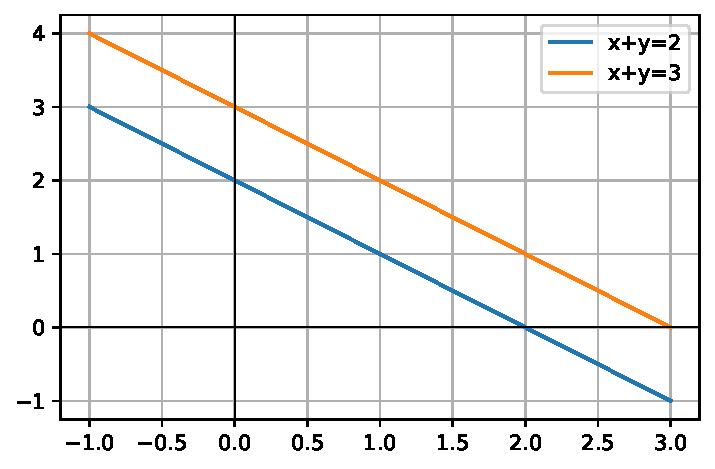
\includegraphics[keepaspectratio]{books/en-US/lab_files/figure-latex/cell-153-output-1.pdf}}

The two lines are parallel → no solution.

\begin{enumerate}
\def\labelenumi{\arabic{enumi}.}
\setcounter{enumi}{3}
\tightlist
\item
  Detecting inconsistency automatically
\end{enumerate}

We can scan the RREF for a row of the form \([0, 0, …, c]\) with
\(c \neq 0\).

\begin{Shaded}
\begin{Highlighting}[]
\KeywordTok{def}\NormalTok{ is\_inconsistent(M):}
\NormalTok{    rref\_matrix, \_ }\OperatorTok{=}\NormalTok{ M.rref()}
    \ControlFlowTok{for}\NormalTok{ row }\KeywordTok{in}\NormalTok{ rref\_matrix.tolist():}
        \ControlFlowTok{if} \BuiltInTok{all}\NormalTok{(v }\OperatorTok{==} \DecValTok{0} \ControlFlowTok{for}\NormalTok{ v }\KeywordTok{in}\NormalTok{ row[:}\OperatorTok{{-}}\DecValTok{1}\NormalTok{]) }\KeywordTok{and}\NormalTok{ row[}\OperatorTok{{-}}\DecValTok{1}\NormalTok{] }\OperatorTok{!=} \DecValTok{0}\NormalTok{:}
            \ControlFlowTok{return} \VariableTok{True}
    \ControlFlowTok{return} \VariableTok{False}

\BuiltInTok{print}\NormalTok{(}\StringTok{"System 1 inconsistent?"}\NormalTok{, is\_inconsistent(M))}
\BuiltInTok{print}\NormalTok{(}\StringTok{"System 2 inconsistent?"}\NormalTok{, is\_inconsistent(M2))}
\end{Highlighting}
\end{Shaded}

\begin{verbatim}
System 1 inconsistent? True
System 2 inconsistent? False
\end{verbatim}

\subsubsection{Try It Yourself}\label{try-it-yourself-124}

\begin{enumerate}
\def\labelenumi{\arabic{enumi}.}
\item
  Test the system:

  \[
  x + 2y = 4, \quad 2x + 4y = 10
  \]

  Write the augmented matrix and check if it's inconsistent.
\item
  Build a random 2×3 augmented matrix with integer entries. Use
  \texttt{is\_inconsistent} to check.
\item
  Plot two linear equations in 2D. Adjust constants to see when they
  intersect (consistent) vs when they are parallel (inconsistent).
\end{enumerate}

\subsubsection{The Takeaway}\label{the-takeaway-8}

\begin{itemize}
\item
  A system is inconsistent if RREF contains a row like \([0,0,…,c]\)
  with \(c \neq 0\).
\item
  Geometrically, this means the equations describe parallel lines (2D),
  parallel planes (3D), or higher-dimensional contradictions.
\item
  Recognizing inconsistency quickly saves time and avoids chasing
  impossible solutions.
\end{itemize}

\subsection{27. Gaussian Elimination by Hand (A Disciplined
Procedure)}\label{gaussian-elimination-by-hand-a-disciplined-procedure}

Gaussian elimination is the systematic way to solve linear systems using
row operations. It transforms the augmented matrix into row-echelon form
(REF) and then uses back substitution to find solutions. In this lab,
we'll walk step by step through the process.

\subsubsection{Set Up Your Lab}\label{set-up-your-lab-26}

\begin{Shaded}
\begin{Highlighting}[]
\ImportTok{import}\NormalTok{ numpy }\ImportTok{as}\NormalTok{ np}
\ImportTok{from}\NormalTok{ sympy }\ImportTok{import}\NormalTok{ Matrix}
\end{Highlighting}
\end{Shaded}

\subsubsection{Step-by-Step Code
Walkthrough}\label{step-by-step-code-walkthrough-26}

\begin{enumerate}
\def\labelenumi{\arabic{enumi}.}
\tightlist
\item
  Example system
\end{enumerate}

\[
\begin{cases}  
x + y + z = 6 \\  
2x + 3y + z = 14 \\  
x + 2y + 3z = 14  
\end{cases}
\]

\begin{Shaded}
\begin{Highlighting}[]
\NormalTok{A }\OperatorTok{=}\NormalTok{ np.array([}
\NormalTok{    [}\DecValTok{1}\NormalTok{, }\DecValTok{1}\NormalTok{, }\DecValTok{1}\NormalTok{, }\DecValTok{6}\NormalTok{],}
\NormalTok{    [}\DecValTok{2}\NormalTok{, }\DecValTok{3}\NormalTok{, }\DecValTok{1}\NormalTok{, }\DecValTok{14}\NormalTok{],}
\NormalTok{    [}\DecValTok{1}\NormalTok{, }\DecValTok{2}\NormalTok{, }\DecValTok{3}\NormalTok{, }\DecValTok{14}\NormalTok{]}
\NormalTok{], dtype}\OperatorTok{=}\BuiltInTok{float}\NormalTok{)}

\BuiltInTok{print}\NormalTok{(}\StringTok{"Initial augmented matrix:}\CharTok{\textbackslash{}n}\StringTok{"}\NormalTok{, A)}
\end{Highlighting}
\end{Shaded}

\begin{verbatim}
Initial augmented matrix:
 [[ 1.  1.  1.  6.]
 [ 2.  3.  1. 14.]
 [ 1.  2.  3. 14.]]
\end{verbatim}

\begin{enumerate}
\def\labelenumi{\arabic{enumi}.}
\setcounter{enumi}{1}
\tightlist
\item
  Step 1: Get a pivot in the first column
\end{enumerate}

Make the pivot at (0,0) into 1 (it already is). Now eliminate below it.

\begin{Shaded}
\begin{Highlighting}[]
\NormalTok{A[}\DecValTok{1}\NormalTok{] }\OperatorTok{=}\NormalTok{ A[}\DecValTok{1}\NormalTok{] }\OperatorTok{{-}} \DecValTok{2}\OperatorTok{*}\NormalTok{A[}\DecValTok{0}\NormalTok{]   }\CommentTok{\# Row2 → Row2 {-} 2*Row1}
\NormalTok{A[}\DecValTok{2}\NormalTok{] }\OperatorTok{=}\NormalTok{ A[}\DecValTok{2}\NormalTok{] }\OperatorTok{{-}}\NormalTok{ A[}\DecValTok{0}\NormalTok{]     }\CommentTok{\# Row3 → Row3 {-} Row1}
\BuiltInTok{print}\NormalTok{(}\StringTok{"After eliminating first column:}\CharTok{\textbackslash{}n}\StringTok{"}\NormalTok{, A)}
\end{Highlighting}
\end{Shaded}

\begin{verbatim}
After eliminating first column:
 [[ 1.  1.  1.  6.]
 [ 0.  1. -1.  2.]
 [ 0.  1.  2.  8.]]
\end{verbatim}

\begin{enumerate}
\def\labelenumi{\arabic{enumi}.}
\setcounter{enumi}{2}
\tightlist
\item
  Step 2: Pivot in the second column
\end{enumerate}

Make the pivot in row 1, col 1 equal to 1.

\begin{Shaded}
\begin{Highlighting}[]
\NormalTok{A[}\DecValTok{1}\NormalTok{] }\OperatorTok{=}\NormalTok{ A[}\DecValTok{1}\NormalTok{] }\OperatorTok{/}\NormalTok{ A[}\DecValTok{1}\NormalTok{,}\DecValTok{1}\NormalTok{]}
\BuiltInTok{print}\NormalTok{(}\StringTok{"After scaling second row:}\CharTok{\textbackslash{}n}\StringTok{"}\NormalTok{, A)}
\end{Highlighting}
\end{Shaded}

\begin{verbatim}
After scaling second row:
 [[ 1.  1.  1.  6.]
 [ 0.  1. -1.  2.]
 [ 0.  1.  2.  8.]]
\end{verbatim}

Now eliminate below:

\begin{Shaded}
\begin{Highlighting}[]
\NormalTok{A[}\DecValTok{2}\NormalTok{] }\OperatorTok{=}\NormalTok{ A[}\DecValTok{2}\NormalTok{] }\OperatorTok{{-}}\NormalTok{ A[}\DecValTok{2}\NormalTok{,}\DecValTok{1}\NormalTok{]}\OperatorTok{*}\NormalTok{A[}\DecValTok{1}\NormalTok{]}
\BuiltInTok{print}\NormalTok{(}\StringTok{"After eliminating second column:}\CharTok{\textbackslash{}n}\StringTok{"}\NormalTok{, A)}
\end{Highlighting}
\end{Shaded}

\begin{verbatim}
After eliminating second column:
 [[ 1.  1.  1.  6.]
 [ 0.  1. -1.  2.]
 [ 0.  0.  3.  6.]]
\end{verbatim}

\begin{enumerate}
\def\labelenumi{\arabic{enumi}.}
\setcounter{enumi}{3}
\tightlist
\item
  Step 3: Pivot in the third column
\end{enumerate}

Make the bottom-right entry into 1.

\begin{Shaded}
\begin{Highlighting}[]
\NormalTok{A[}\DecValTok{2}\NormalTok{] }\OperatorTok{=}\NormalTok{ A[}\DecValTok{2}\NormalTok{] }\OperatorTok{/}\NormalTok{ A[}\DecValTok{2}\NormalTok{,}\DecValTok{2}\NormalTok{]}
\BuiltInTok{print}\NormalTok{(}\StringTok{"After scaling third row:}\CharTok{\textbackslash{}n}\StringTok{"}\NormalTok{, A)}
\end{Highlighting}
\end{Shaded}

\begin{verbatim}
After scaling third row:
 [[ 1.  1.  1.  6.]
 [ 0.  1. -1.  2.]
 [ 0.  0.  1.  2.]]
\end{verbatim}

At this point, the matrix is in row-echelon form (REF).

\begin{enumerate}
\def\labelenumi{\arabic{enumi}.}
\setcounter{enumi}{4}
\tightlist
\item
  Back substitution
\end{enumerate}

Now solve from the bottom up:

\begin{Shaded}
\begin{Highlighting}[]
\NormalTok{z }\OperatorTok{=}\NormalTok{ A[}\DecValTok{2}\NormalTok{,}\DecValTok{3}\NormalTok{]}
\NormalTok{y }\OperatorTok{=}\NormalTok{ A[}\DecValTok{1}\NormalTok{,}\DecValTok{3}\NormalTok{] }\OperatorTok{{-}}\NormalTok{ A[}\DecValTok{1}\NormalTok{,}\DecValTok{2}\NormalTok{]}\OperatorTok{*}\NormalTok{z}
\NormalTok{x }\OperatorTok{=}\NormalTok{ A[}\DecValTok{0}\NormalTok{,}\DecValTok{3}\NormalTok{] }\OperatorTok{{-}}\NormalTok{ A[}\DecValTok{0}\NormalTok{,}\DecValTok{1}\NormalTok{]}\OperatorTok{*}\NormalTok{y }\OperatorTok{{-}}\NormalTok{ A[}\DecValTok{0}\NormalTok{,}\DecValTok{2}\NormalTok{]}\OperatorTok{*}\NormalTok{z}

\BuiltInTok{print}\NormalTok{(}\SpecialStringTok{f"Solution: x=}\SpecialCharTok{\{}\NormalTok{x}\SpecialCharTok{\}}\SpecialStringTok{, y=}\SpecialCharTok{\{}\NormalTok{y}\SpecialCharTok{\}}\SpecialStringTok{, z=}\SpecialCharTok{\{}\NormalTok{z}\SpecialCharTok{\}}\SpecialStringTok{"}\NormalTok{)}
\end{Highlighting}
\end{Shaded}

\begin{verbatim}
Solution: x=0.0, y=4.0, z=2.0
\end{verbatim}

\begin{enumerate}
\def\labelenumi{\arabic{enumi}.}
\setcounter{enumi}{5}
\tightlist
\item
  Verification
\end{enumerate}

\begin{Shaded}
\begin{Highlighting}[]
\NormalTok{coeff }\OperatorTok{=}\NormalTok{ np.array([}
\NormalTok{    [}\DecValTok{1}\NormalTok{,}\DecValTok{1}\NormalTok{,}\DecValTok{1}\NormalTok{],}
\NormalTok{    [}\DecValTok{2}\NormalTok{,}\DecValTok{3}\NormalTok{,}\DecValTok{1}\NormalTok{],}
\NormalTok{    [}\DecValTok{1}\NormalTok{,}\DecValTok{2}\NormalTok{,}\DecValTok{3}\NormalTok{]}
\NormalTok{], dtype}\OperatorTok{=}\BuiltInTok{float}\NormalTok{)}
\NormalTok{const }\OperatorTok{=}\NormalTok{ np.array([}\DecValTok{6}\NormalTok{,}\DecValTok{14}\NormalTok{,}\DecValTok{14}\NormalTok{], dtype}\OperatorTok{=}\BuiltInTok{float}\NormalTok{)}

\BuiltInTok{print}\NormalTok{(}\StringTok{"Check with np.linalg.solve:"}\NormalTok{, np.linalg.solve(coeff,const))}
\end{Highlighting}
\end{Shaded}

\begin{verbatim}
Check with np.linalg.solve: [0. 4. 2.]
\end{verbatim}

The results match.

\subsubsection{Try It Yourself}\label{try-it-yourself-125}

\begin{enumerate}
\def\labelenumi{\arabic{enumi}.}
\item
  Solve:

  \[
  2x + y = 5, \quad 4x - 6y = -2
  \]

  using Gaussian elimination manually in code.
\item
  Create a random 3×4 augmented matrix and reduce it step by step,
  printing after each row operation.
\item
  Compare your manual elimination to SymPy's RREF with
  \texttt{Matrix.rref()}.
\end{enumerate}

\subsubsection{The Takeaway}\label{the-takeaway-9}

\begin{itemize}
\tightlist
\item
  Gaussian elimination is a disciplined sequence of row operations.
\item
  It reduces the matrix to row-echelon form, from which back
  substitution is straightforward.
\item
  This method is the backbone of solving systems by hand and underlies
  many numerical algorithms.
\end{itemize}

\subsection{28. Back Substitution and Solution Sets (Finishing
Cleanly)}\label{back-substitution-and-solution-sets-finishing-cleanly}

Once Gaussian elimination reduces a system to row-echelon form (REF),
the final step is back substitution. This means solving variables
starting from the last equation and working upward. In this lab, we'll
practice both unique and infinite solution cases.

\subsubsection{Set Up Your Lab}\label{set-up-your-lab-27}

\begin{Shaded}
\begin{Highlighting}[]
\ImportTok{import}\NormalTok{ numpy }\ImportTok{as}\NormalTok{ np}
\ImportTok{from}\NormalTok{ sympy }\ImportTok{import}\NormalTok{ Matrix}
\end{Highlighting}
\end{Shaded}

\subsubsection{Step-by-Step Code
Walkthrough}\label{step-by-step-code-walkthrough-27}

\begin{enumerate}
\def\labelenumi{\arabic{enumi}.}
\tightlist
\item
  Unique solution example
\end{enumerate}

System:

\[
x + y + z = 6, \quad 2y + 5z = -4, \quad z = 3
\]

Row-echelon form looks like:

\[
\begin{bmatrix}  
1 & 1 & 1 & 6 \\  
0 & 2 & 5 & -4 \\  
0 & 0 & 1 & 3  
\end{bmatrix}
\]

Solve bottom-up:

\begin{Shaded}
\begin{Highlighting}[]
\NormalTok{z }\OperatorTok{=} \DecValTok{3}
\NormalTok{y }\OperatorTok{=}\NormalTok{ (}\OperatorTok{{-}}\DecValTok{4} \OperatorTok{{-}} \DecValTok{5}\OperatorTok{*}\NormalTok{z)}\OperatorTok{/}\DecValTok{2}
\NormalTok{x }\OperatorTok{=} \DecValTok{6} \OperatorTok{{-}}\NormalTok{ y }\OperatorTok{{-}}\NormalTok{ z}
\BuiltInTok{print}\NormalTok{(}\SpecialStringTok{f"Solution: x=}\SpecialCharTok{\{}\NormalTok{x}\SpecialCharTok{\}}\SpecialStringTok{, y=}\SpecialCharTok{\{}\NormalTok{y}\SpecialCharTok{\}}\SpecialStringTok{, z=}\SpecialCharTok{\{}\NormalTok{z}\SpecialCharTok{\}}\SpecialStringTok{"}\NormalTok{)}
\end{Highlighting}
\end{Shaded}

\begin{verbatim}
Solution: x=12.5, y=-9.5, z=3
\end{verbatim}

\begin{enumerate}
\def\labelenumi{\arabic{enumi}.}
\setcounter{enumi}{1}
\tightlist
\item
  Infinite solution example
\end{enumerate}

System:

\[
x + y + z = 2, \quad 2x + 2y + 2z = 4
\]

After elimination:

\[
\begin{bmatrix}  
1 & 1 & 1 & 2 \\  
0 & 0 & 0 & 0  
\end{bmatrix}
\]

This means:

\begin{itemize}
\tightlist
\item
  Equation: \(x + y + z = 2\).
\item
  Free variables: choose \(y\) and \(z\).
\end{itemize}

Let \(y = s, z = t\). Then:

\[
x = 2 - s - t
\]

So the solution set is:

\begin{Shaded}
\begin{Highlighting}[]
\ImportTok{from}\NormalTok{ sympy }\ImportTok{import}\NormalTok{ symbols}
\NormalTok{s, t }\OperatorTok{=}\NormalTok{ symbols(}\StringTok{\textquotesingle{}s t\textquotesingle{}}\NormalTok{)}
\NormalTok{x }\OperatorTok{=} \DecValTok{2} \OperatorTok{{-}}\NormalTok{ s }\OperatorTok{{-}}\NormalTok{ t}
\NormalTok{y }\OperatorTok{=}\NormalTok{ s}
\NormalTok{z }\OperatorTok{=}\NormalTok{ t}
\BuiltInTok{print}\NormalTok{(}\StringTok{"General solution:"}\NormalTok{)}
\BuiltInTok{print}\NormalTok{(}\StringTok{"x ="}\NormalTok{, x, }\StringTok{", y ="}\NormalTok{, y, }\StringTok{", z ="}\NormalTok{, z)}
\end{Highlighting}
\end{Shaded}

\begin{verbatim}
General solution:
x = -s - t + 2 , y = s , z = t
\end{verbatim}

\begin{enumerate}
\def\labelenumi{\arabic{enumi}.}
\setcounter{enumi}{2}
\tightlist
\item
  Consistency check with RREF
\end{enumerate}

We can use SymPy to confirm solution sets:

\begin{Shaded}
\begin{Highlighting}[]
\NormalTok{M }\OperatorTok{=}\NormalTok{ Matrix([}
\NormalTok{    [}\DecValTok{1}\NormalTok{,}\DecValTok{1}\NormalTok{,}\DecValTok{1}\NormalTok{,}\DecValTok{2}\NormalTok{],}
\NormalTok{    [}\DecValTok{2}\NormalTok{,}\DecValTok{2}\NormalTok{,}\DecValTok{2}\NormalTok{,}\DecValTok{4}\NormalTok{]}
\NormalTok{])}

\BuiltInTok{print}\NormalTok{(}\StringTok{"RREF form:}\CharTok{\textbackslash{}n}\StringTok{"}\NormalTok{, M.rref()[}\DecValTok{0}\NormalTok{])}
\end{Highlighting}
\end{Shaded}

\begin{verbatim}
RREF form:
 Matrix([[1, 1, 1, 2], [0, 0, 0, 0]])
\end{verbatim}

The second row disappears, showing infinite solutions.

\begin{enumerate}
\def\labelenumi{\arabic{enumi}.}
\setcounter{enumi}{3}
\tightlist
\item
  Encoding solution sets
\end{enumerate}

General solutions are often written in parametric vector form.

For the infinite solution above:

\[
(x,y,z) = (2,0,0) + s(-1,1,0) + t(-1,0,1)
\]

This shows the solution space is a plane in \(\mathbb{R}^3\).

\subsubsection{Try It Yourself}\label{try-it-yourself-126}

\begin{enumerate}
\def\labelenumi{\arabic{enumi}.}
\item
  Solve:

  \[
  x + 2y = 5, \quad y = 1
  \]

  Do back substitution by hand and check with NumPy.
\item
  Take the system:

  \[
  x + y + z = 1, \quad 2x + 2y + 2z = 2
  \]

  Write its solution set in parametric form.
\item
  Use \texttt{Matrix.rref()} on a 3×4 random augmented matrix. Identify
  pivot and free variables, then describe the solution set.
\end{enumerate}

\subsubsection{The Takeaway}\label{the-takeaway-10}

\begin{itemize}
\tightlist
\item
  Back substitution is the cleanup step after Gaussian elimination.
\item
  It reveals whether the system has a unique solution or infinitely
  many.
\item
  Solutions can be expressed explicitly (unique case) or parametrically
  (infinite case).
\end{itemize}

\subsection{29. Rank and Its First Meaning (Pivots as
Information)}\label{rank-and-its-first-meaning-pivots-as-information}

The rank of a matrix tells us how much independent information it
contains. Rank is one of the most important concepts in linear algebra
because it connects to pivots, independence, dimension, and the number
of solutions to a system.

\subsubsection{Set Up Your Lab}\label{set-up-your-lab-28}

\begin{Shaded}
\begin{Highlighting}[]
\ImportTok{import}\NormalTok{ numpy }\ImportTok{as}\NormalTok{ np}
\ImportTok{from}\NormalTok{ sympy }\ImportTok{import}\NormalTok{ Matrix}
\end{Highlighting}
\end{Shaded}

\subsubsection{Step-by-Step Code
Walkthrough}\label{step-by-step-code-walkthrough-28}

\begin{enumerate}
\def\labelenumi{\arabic{enumi}.}
\tightlist
\item
  Rank definition The rank is the number of pivots (leading ones) in the
  row-echelon form of a matrix.
\end{enumerate}

Example:

\begin{Shaded}
\begin{Highlighting}[]
\NormalTok{A }\OperatorTok{=}\NormalTok{ Matrix([}
\NormalTok{    [}\DecValTok{1}\NormalTok{, }\DecValTok{2}\NormalTok{, }\DecValTok{3}\NormalTok{],}
\NormalTok{    [}\DecValTok{2}\NormalTok{, }\DecValTok{4}\NormalTok{, }\DecValTok{6}\NormalTok{],}
\NormalTok{    [}\DecValTok{1}\NormalTok{, }\DecValTok{1}\NormalTok{, }\DecValTok{1}\NormalTok{]}
\NormalTok{])}

\BuiltInTok{print}\NormalTok{(}\StringTok{"RREF:}\CharTok{\textbackslash{}n}\StringTok{"}\NormalTok{, A.rref()[}\DecValTok{0}\NormalTok{])}
\BuiltInTok{print}\NormalTok{(}\StringTok{"Rank of A:"}\NormalTok{, A.rank())}
\end{Highlighting}
\end{Shaded}

\begin{verbatim}
RREF:
 Matrix([[1, 0, -1], [0, 1, 2], [0, 0, 0]])
Rank of A: 2
\end{verbatim}

\begin{itemize}
\tightlist
\item
  The second row is a multiple of the first, so the rank is less than 3.
\item
  Only two independent rows → rank = 2.
\end{itemize}

\begin{enumerate}
\def\labelenumi{\arabic{enumi}.}
\setcounter{enumi}{1}
\tightlist
\item
  Rank and solutions to \(A·x = b\)
\end{enumerate}

Consider:

\[
\begin{cases}  
x + y + z = 3 \\  
2x + 2y + 2z = 6 \\  
x - y = 0  
\end{cases}
\]

\begin{Shaded}
\begin{Highlighting}[]
\NormalTok{M }\OperatorTok{=}\NormalTok{ Matrix([}
\NormalTok{    [}\DecValTok{1}\NormalTok{, }\DecValTok{1}\NormalTok{, }\DecValTok{1}\NormalTok{, }\DecValTok{3}\NormalTok{],}
\NormalTok{    [}\DecValTok{2}\NormalTok{, }\DecValTok{2}\NormalTok{, }\DecValTok{2}\NormalTok{, }\DecValTok{6}\NormalTok{],}
\NormalTok{    [}\DecValTok{1}\NormalTok{, }\OperatorTok{{-}}\DecValTok{1}\NormalTok{, }\DecValTok{0}\NormalTok{, }\DecValTok{0}\NormalTok{]}
\NormalTok{])}

\BuiltInTok{print}\NormalTok{(}\StringTok{"RREF:}\CharTok{\textbackslash{}n}\StringTok{"}\NormalTok{, M.rref()[}\DecValTok{0}\NormalTok{])}
\BuiltInTok{print}\NormalTok{(}\StringTok{"Rank of coefficient matrix:"}\NormalTok{, M[:, :}\OperatorTok{{-}}\DecValTok{1}\NormalTok{].rank())}
\BuiltInTok{print}\NormalTok{(}\StringTok{"Rank of augmented matrix:"}\NormalTok{, M.rank())}
\end{Highlighting}
\end{Shaded}

\begin{verbatim}
RREF:
 Matrix([[1, 0, 1/2, 3/2], [0, 1, 1/2, 3/2], [0, 0, 0, 0]])
Rank of coefficient matrix: 2
Rank of augmented matrix: 2
\end{verbatim}

\begin{itemize}
\tightlist
\item
  If rank(A) = rank({[}A\textbar b{]}) = number of variables → unique
  solution.
\item
  If rank(A) = rank({[}A\textbar b{]}) \textless{} number of variables →
  infinite solutions.
\item
  If rank(A) \textless{} rank({[}A\textbar b{]}) → no solution.
\end{itemize}

\begin{enumerate}
\def\labelenumi{\arabic{enumi}.}
\setcounter{enumi}{2}
\tightlist
\item
  NumPy comparison
\end{enumerate}

\begin{Shaded}
\begin{Highlighting}[]
\NormalTok{A }\OperatorTok{=}\NormalTok{ np.array([}
\NormalTok{    [}\DecValTok{1}\NormalTok{, }\DecValTok{2}\NormalTok{, }\DecValTok{3}\NormalTok{],}
\NormalTok{    [}\DecValTok{2}\NormalTok{, }\DecValTok{4}\NormalTok{, }\DecValTok{6}\NormalTok{],}
\NormalTok{    [}\DecValTok{1}\NormalTok{, }\DecValTok{1}\NormalTok{, }\DecValTok{1}\NormalTok{]}
\NormalTok{], dtype}\OperatorTok{=}\BuiltInTok{float}\NormalTok{)}

\BuiltInTok{print}\NormalTok{(}\StringTok{"Rank with NumPy:"}\NormalTok{, np.linalg.matrix\_rank(A))}
\end{Highlighting}
\end{Shaded}

\begin{verbatim}
Rank with NumPy: 2
\end{verbatim}

\begin{enumerate}
\def\labelenumi{\arabic{enumi}.}
\setcounter{enumi}{3}
\tightlist
\item
  Rank as ``dimension of information''
\end{enumerate}

The rank equals:

\begin{itemize}
\tightlist
\item
  The number of independent rows.
\item
  The number of independent columns.
\item
  The dimension of the column space.
\end{itemize}

\begin{Shaded}
\begin{Highlighting}[]
\NormalTok{B }\OperatorTok{=}\NormalTok{ Matrix([}
\NormalTok{    [}\DecValTok{1}\NormalTok{,}\DecValTok{2}\NormalTok{],}
\NormalTok{    [}\DecValTok{2}\NormalTok{,}\DecValTok{4}\NormalTok{],}
\NormalTok{    [}\DecValTok{3}\NormalTok{,}\DecValTok{6}\NormalTok{]}
\NormalTok{])}

\BuiltInTok{print}\NormalTok{(}\StringTok{"Rank of B:"}\NormalTok{, B.rank())}
\end{Highlighting}
\end{Shaded}

\begin{verbatim}
Rank of B: 1
\end{verbatim}

All columns are multiples → only one independent direction → rank = 1.

\subsubsection{Try It Yourself}\label{try-it-yourself-127}

\begin{enumerate}
\def\labelenumi{\arabic{enumi}.}
\item
  Compute the rank of:

  \[
  \begin{bmatrix}  
  1 & 2 & 3 \\  
  2 & 4 & 6 \\  
  3 & 6 & 9  
  \end{bmatrix}
  \]

  What do you expect?
\item
  Create a random 4×4 matrix with \texttt{np.random.randint}. Compute
  its rank with both SymPy and NumPy.
\item
  Test solution consistency using rank: build a system where rank(A) ≠
  rank({[}A\textbar b{]}) and show it has no solution.
\end{enumerate}

\subsubsection{The Takeaway}\label{the-takeaway-11}

\begin{itemize}
\tightlist
\item
  Rank = number of pivots = dimension of independent information.
\item
  Rank reveals whether a system has no solution, one solution, or
  infinitely many.
\item
  Rank connects algebra (pivots) with geometry (dimension of subspaces).
\end{itemize}

\subsection{30. LU Factorization (Elimination Captured as L and
U)}\label{lu-factorization-elimination-captured-as-l-and-u}

Gaussian elimination can be recorded in a neat factorization:

\[
A = LU
\]

where \(L\) is a lower triangular matrix (recording the multipliers we
used) and \(U\) is an upper triangular matrix (the result of
elimination). This is called LU factorization. It's a powerful tool for
solving systems efficiently.

\subsubsection{Set Up Your Lab}\label{set-up-your-lab-29}

\begin{Shaded}
\begin{Highlighting}[]
\ImportTok{import}\NormalTok{ numpy }\ImportTok{as}\NormalTok{ np}
\ImportTok{from}\NormalTok{ scipy.linalg }\ImportTok{import}\NormalTok{ lu}
\end{Highlighting}
\end{Shaded}

\subsubsection{Step-by-Step Code
Walkthrough}\label{step-by-step-code-walkthrough-29}

\begin{enumerate}
\def\labelenumi{\arabic{enumi}.}
\tightlist
\item
  Example matrix
\end{enumerate}

\begin{Shaded}
\begin{Highlighting}[]
\NormalTok{A }\OperatorTok{=}\NormalTok{ np.array([}
\NormalTok{    [}\DecValTok{2}\NormalTok{, }\DecValTok{3}\NormalTok{, }\DecValTok{1}\NormalTok{],}
\NormalTok{    [}\DecValTok{4}\NormalTok{, }\DecValTok{7}\NormalTok{, }\DecValTok{7}\NormalTok{],}
\NormalTok{    [}\DecValTok{6}\NormalTok{, }\DecValTok{18}\NormalTok{, }\DecValTok{22}\NormalTok{]}
\NormalTok{], dtype}\OperatorTok{=}\BuiltInTok{float}\NormalTok{)}

\BuiltInTok{print}\NormalTok{(}\StringTok{"Matrix A:}\CharTok{\textbackslash{}n}\StringTok{"}\NormalTok{, A)}
\end{Highlighting}
\end{Shaded}

\begin{verbatim}
Matrix A:
 [[ 2.  3.  1.]
 [ 4.  7.  7.]
 [ 6. 18. 22.]]
\end{verbatim}

\begin{enumerate}
\def\labelenumi{\arabic{enumi}.}
\setcounter{enumi}{1}
\tightlist
\item
  LU decomposition with SciPy
\end{enumerate}

\begin{Shaded}
\begin{Highlighting}[]
\NormalTok{P, L, U }\OperatorTok{=}\NormalTok{ lu(A)}

\BuiltInTok{print}\NormalTok{(}\StringTok{"Permutation matrix P:}\CharTok{\textbackslash{}n}\StringTok{"}\NormalTok{, P)}
\BuiltInTok{print}\NormalTok{(}\StringTok{"Lower triangular L:}\CharTok{\textbackslash{}n}\StringTok{"}\NormalTok{, L)}
\BuiltInTok{print}\NormalTok{(}\StringTok{"Upper triangular U:}\CharTok{\textbackslash{}n}\StringTok{"}\NormalTok{, U)}
\end{Highlighting}
\end{Shaded}

\begin{verbatim}
Permutation matrix P:
 [[0. 0. 1.]
 [0. 1. 0.]
 [1. 0. 0.]]
Lower triangular L:
 [[1.         0.         0.        ]
 [0.66666667 1.         0.        ]
 [0.33333333 0.6        1.        ]]
Upper triangular U:
 [[ 6.         18.         22.        ]
 [ 0.         -5.         -7.66666667]
 [ 0.          0.         -1.73333333]]
\end{verbatim}

Here, \(P\) handles row swaps (partial pivoting), \(L\) is lower
triangular, and \(U\) is upper triangular.

\begin{enumerate}
\def\labelenumi{\arabic{enumi}.}
\setcounter{enumi}{2}
\tightlist
\item
  Verifying the factorization
\end{enumerate}

\begin{Shaded}
\begin{Highlighting}[]
\NormalTok{reconstructed }\OperatorTok{=}\NormalTok{ P }\OperatorTok{@}\NormalTok{ L }\OperatorTok{@}\NormalTok{ U}
\BuiltInTok{print}\NormalTok{(}\StringTok{"Does P·L·U equal A?}\CharTok{\textbackslash{}n}\StringTok{"}\NormalTok{, np.allclose(reconstructed, A))}
\end{Highlighting}
\end{Shaded}

\begin{verbatim}
Does P·L·U equal A?
 True
\end{verbatim}

\begin{enumerate}
\def\labelenumi{\arabic{enumi}.}
\setcounter{enumi}{3}
\tightlist
\item
  Solving a system with LU
\end{enumerate}

Suppose we want to solve \(Ax = b\). Instead of working directly with
\(A\), we solve in two steps:

\begin{enumerate}
\def\labelenumi{\arabic{enumi}.}
\tightlist
\item
  Solve \(Ly = Pb\) (forward substitution).
\item
  Solve \(Ux = y\) (back substitution).
\end{enumerate}

\begin{Shaded}
\begin{Highlighting}[]
\NormalTok{b }\OperatorTok{=}\NormalTok{ np.array([}\DecValTok{1}\NormalTok{, }\DecValTok{2}\NormalTok{, }\DecValTok{3}\NormalTok{], dtype}\OperatorTok{=}\BuiltInTok{float}\NormalTok{)}

\CommentTok{\# Step 1: Pb}
\NormalTok{Pb }\OperatorTok{=}\NormalTok{ P }\OperatorTok{@}\NormalTok{ b}

\CommentTok{\# Step 2: forward substitution Ly = Pb}
\NormalTok{y }\OperatorTok{=}\NormalTok{ np.linalg.solve(L, Pb)}

\CommentTok{\# Step 3: back substitution Ux = y}
\NormalTok{x }\OperatorTok{=}\NormalTok{ np.linalg.solve(U, y)}

\BuiltInTok{print}\NormalTok{(}\StringTok{"Solution x:"}\NormalTok{, x)}
\end{Highlighting}
\end{Shaded}

\begin{verbatim}
Solution x: [ 0.5 -0.  -0. ]
\end{verbatim}

\begin{enumerate}
\def\labelenumi{\arabic{enumi}.}
\setcounter{enumi}{4}
\tightlist
\item
  Efficiency advantage
\end{enumerate}

If we have to solve many systems with the same \(A\) but different
\(b\), we only compute \(LU\) once, then reuse it. This saves a lot of
computation.

\begin{enumerate}
\def\labelenumi{\arabic{enumi}.}
\setcounter{enumi}{5}
\tightlist
\item
  NumPy's built-in rank-revealing factorization
\end{enumerate}

While NumPy doesn't have \texttt{lu} directly, it works seamlessly with
SciPy. For large matrices, LU decomposition is the backbone of solvers
like \texttt{np.linalg.solve}.

\subsubsection{Try It Yourself}\label{try-it-yourself-128}

\begin{enumerate}
\def\labelenumi{\arabic{enumi}.}
\item
  Compute LU decomposition for

  \[
  A = \begin{bmatrix} 1 & 2 & 0 \\ 3 & 4 & 4 \\ 5 & 6 & 3 \end{bmatrix}
  \]

  Verify \(P·L·U = A\).
\item
  Solve \(Ax = b\) with

  \[
  b = [3,7,8]
  \]

  using LU factorization.
\item
  Compare solving with LU factorization vs directly using
  \texttt{np.linalg.solve(A,b)}. Are the answers the same?
\end{enumerate}

\subsubsection{The Takeaway}\label{the-takeaway-12}

\begin{itemize}
\tightlist
\item
  LU factorization captures Gaussian elimination in matrix form:
  \(A = P·L·U\).
\item
  It allows fast repeated solving of systems with different right-hand
  sides.
\item
  LU decomposition is a core technique in numerical linear algebra and
  the basis of many solvers.
\end{itemize}

\section{Chapter 4. Vector Spaces and
Subspaces}\label{chapter-4.-vector-spaces-and-subspaces-2}

\subsection{31. Axioms of Vector Spaces (What ``Space'' Really
Means)}\label{axioms-of-vector-spaces-what-space-really-means}

Vector spaces generalize what we've been doing with vectors and
matrices. Instead of just \(\mathbb{R}^n\), a vector space is any
collection of objects (vectors) where addition and scalar multiplication
follow specific axioms (rules). In this lab, we'll explore these axioms
concretely with Python.

\subsubsection{Set Up Your Lab}\label{set-up-your-lab-30}

\begin{Shaded}
\begin{Highlighting}[]
\ImportTok{import}\NormalTok{ numpy }\ImportTok{as}\NormalTok{ np}
\end{Highlighting}
\end{Shaded}

\subsubsection{Step-by-Step Code
Walkthrough}\label{step-by-step-code-walkthrough-30}

\begin{enumerate}
\def\labelenumi{\arabic{enumi}.}
\tightlist
\item
  Vector space example: \(\mathbb{R}^2\)
\end{enumerate}

Let's check two rules (axioms): closure under addition and scalar
multiplication.

\begin{Shaded}
\begin{Highlighting}[]
\NormalTok{u }\OperatorTok{=}\NormalTok{ np.array([}\DecValTok{1}\NormalTok{, }\DecValTok{2}\NormalTok{])}
\NormalTok{v }\OperatorTok{=}\NormalTok{ np.array([}\DecValTok{3}\NormalTok{, }\OperatorTok{{-}}\DecValTok{1}\NormalTok{])}

\CommentTok{\# Closure under addition}
\BuiltInTok{print}\NormalTok{(}\StringTok{"u + v ="}\NormalTok{, u }\OperatorTok{+}\NormalTok{ v)}

\CommentTok{\# Closure under scalar multiplication}
\NormalTok{k }\OperatorTok{=} \DecValTok{5}
\BuiltInTok{print}\NormalTok{(}\StringTok{"k * u ="}\NormalTok{, k }\OperatorTok{*}\NormalTok{ u)}
\end{Highlighting}
\end{Shaded}

\begin{verbatim}
u + v = [4 1]
k * u = [ 5 10]
\end{verbatim}

Both results are still in \(\mathbb{R}^2\).

\begin{enumerate}
\def\labelenumi{\arabic{enumi}.}
\setcounter{enumi}{1}
\tightlist
\item
  Zero vector and additive inverses
\end{enumerate}

Every vector space must contain a zero vector, and every vector must
have an additive inverse.

\begin{Shaded}
\begin{Highlighting}[]
\NormalTok{zero }\OperatorTok{=}\NormalTok{ np.array([}\DecValTok{0}\NormalTok{, }\DecValTok{0}\NormalTok{])}
\NormalTok{inverse\_u }\OperatorTok{=} \OperatorTok{{-}}\NormalTok{u}
\BuiltInTok{print}\NormalTok{(}\StringTok{"Zero vector:"}\NormalTok{, zero)}
\BuiltInTok{print}\NormalTok{(}\StringTok{"u + ({-}u) ="}\NormalTok{, u }\OperatorTok{+}\NormalTok{ inverse\_u)}
\end{Highlighting}
\end{Shaded}

\begin{verbatim}
Zero vector: [0 0]
u + (-u) = [0 0]
\end{verbatim}

\begin{enumerate}
\def\labelenumi{\arabic{enumi}.}
\setcounter{enumi}{2}
\tightlist
\item
  Distributive and associative properties
\end{enumerate}

Check:

\begin{itemize}
\tightlist
\item
  \(a(u+v) = au + av\)
\item
  \((a+b)u = au + bu\)
\end{itemize}

\begin{Shaded}
\begin{Highlighting}[]
\NormalTok{a, b }\OperatorTok{=} \DecValTok{2}\NormalTok{, }\DecValTok{3}

\NormalTok{lhs1 }\OperatorTok{=}\NormalTok{ a }\OperatorTok{*}\NormalTok{ (u }\OperatorTok{+}\NormalTok{ v)}
\NormalTok{rhs1 }\OperatorTok{=}\NormalTok{ a}\OperatorTok{*}\NormalTok{u }\OperatorTok{+}\NormalTok{ a}\OperatorTok{*}\NormalTok{v}
\BuiltInTok{print}\NormalTok{(}\StringTok{"a(u+v) ="}\NormalTok{, lhs1, }\StringTok{", au+av ="}\NormalTok{, rhs1)}

\NormalTok{lhs2 }\OperatorTok{=}\NormalTok{ (a}\OperatorTok{+}\NormalTok{b) }\OperatorTok{*}\NormalTok{ u}
\NormalTok{rhs2 }\OperatorTok{=}\NormalTok{ a}\OperatorTok{*}\NormalTok{u }\OperatorTok{+}\NormalTok{ b}\OperatorTok{*}\NormalTok{u}
\BuiltInTok{print}\NormalTok{(}\StringTok{"(a+b)u ="}\NormalTok{, lhs2, }\StringTok{", au+bu ="}\NormalTok{, rhs2)}
\end{Highlighting}
\end{Shaded}

\begin{verbatim}
a(u+v) = [8 2] , au+av = [8 2]
(a+b)u = [ 5 10] , au+bu = [ 5 10]
\end{verbatim}

Both equalities hold → distributive laws confirmed.

\begin{enumerate}
\def\labelenumi{\arabic{enumi}.}
\setcounter{enumi}{3}
\tightlist
\item
  A set that fails to be a vector space
\end{enumerate}

Consider only positive numbers with normal addition and scalar
multiplication.

\begin{Shaded}
\begin{Highlighting}[]
\NormalTok{positive\_numbers }\OperatorTok{=}\NormalTok{ [}\DecValTok{1}\NormalTok{, }\DecValTok{2}\NormalTok{, }\DecValTok{3}\NormalTok{]}
\ControlFlowTok{try}\NormalTok{:}
    \BuiltInTok{print}\NormalTok{(}\StringTok{"Closure under negatives?"}\NormalTok{, }\OperatorTok{{-}}\DecValTok{1} \OperatorTok{*}\NormalTok{ np.array(positive\_numbers))}
\ControlFlowTok{except} \PreprocessorTok{Exception} \ImportTok{as}\NormalTok{ e:}
    \BuiltInTok{print}\NormalTok{(}\StringTok{"Error:"}\NormalTok{, e)}
\end{Highlighting}
\end{Shaded}

\begin{verbatim}
Closure under negatives? [-1 -2 -3]
\end{verbatim}

Negative results leave the set → not a vector space.

\begin{enumerate}
\def\labelenumi{\arabic{enumi}.}
\setcounter{enumi}{4}
\tightlist
\item
  Python helper to check axioms
\end{enumerate}

We can quickly check if a set of vectors is closed under addition and
scalar multiplication.

\begin{Shaded}
\begin{Highlighting}[]
\KeywordTok{def}\NormalTok{ check\_closure(vectors, scalars):}
    \ControlFlowTok{for}\NormalTok{ v }\KeywordTok{in}\NormalTok{ vectors:}
        \ControlFlowTok{for}\NormalTok{ u }\KeywordTok{in}\NormalTok{ vectors:}
            \ControlFlowTok{if} \KeywordTok{not} \BuiltInTok{any}\NormalTok{(np.array\_equal(v}\OperatorTok{+}\NormalTok{u, w) }\ControlFlowTok{for}\NormalTok{ w }\KeywordTok{in}\NormalTok{ vectors):}
                \ControlFlowTok{return} \VariableTok{False}
        \ControlFlowTok{for}\NormalTok{ k }\KeywordTok{in}\NormalTok{ scalars:}
            \ControlFlowTok{if} \KeywordTok{not} \BuiltInTok{any}\NormalTok{(np.array\_equal(k}\OperatorTok{*}\NormalTok{v, w) }\ControlFlowTok{for}\NormalTok{ w }\KeywordTok{in}\NormalTok{ vectors):}
                \ControlFlowTok{return} \VariableTok{False}
    \ControlFlowTok{return} \VariableTok{True}

\NormalTok{vectors }\OperatorTok{=}\NormalTok{ [np.array([}\DecValTok{0}\NormalTok{,}\DecValTok{0}\NormalTok{]), np.array([}\DecValTok{1}\NormalTok{,}\DecValTok{0}\NormalTok{]), np.array([}\DecValTok{0}\NormalTok{,}\DecValTok{1}\NormalTok{]), np.array([}\DecValTok{1}\NormalTok{,}\DecValTok{1}\NormalTok{])]}
\NormalTok{scalars }\OperatorTok{=}\NormalTok{ [}\DecValTok{0}\NormalTok{,}\DecValTok{1}\NormalTok{,}\OperatorTok{{-}}\DecValTok{1}\NormalTok{]}
\BuiltInTok{print}\NormalTok{(}\StringTok{"Closed under addition and scalar multiplication?"}\NormalTok{, check\_closure(vectors, scalars))}
\end{Highlighting}
\end{Shaded}

\begin{verbatim}
Closed under addition and scalar multiplication? False
\end{verbatim}

This small set is closed → it forms a vector space (a subspace of
\(\mathbb{R}^2\)).

\subsubsection{Try It Yourself}\label{try-it-yourself-129}

\begin{enumerate}
\def\labelenumi{\arabic{enumi}.}
\tightlist
\item
  Verify that \(\mathbb{R}^3\) satisfies the vector space axioms using
  random vectors.
\item
  Test whether the set of all 2×2 matrices forms a vector space under
  normal addition and scalar multiplication.
\item
  Find an example of a set that fails closure (e.g., integers under
  division).
\end{enumerate}

\subsubsection{The Takeaway}\label{the-takeaway-13}

\begin{itemize}
\tightlist
\item
  A vector space is any set where addition and scalar multiplication
  satisfy 10 standard axioms.
\item
  These rules ensure consistent algebraic behavior.
\item
  Many objects beyond arrows in \(\mathbb{R}^n\) (like polynomials or
  matrices) are vector spaces too.
\end{itemize}

\subsection{32. Subspaces, Column Space, and Null Space (Where Solutions
Live)}\label{subspaces-column-space-and-null-space-where-solutions-live}

A subspace is a smaller vector space sitting inside a bigger one. For
matrices, two subspaces show up all the time:

\begin{itemize}
\tightlist
\item
  Column space: all combinations of the matrix's columns (possible
  outputs of \(Ax\)).
\item
  Null space: all vectors \(x\) such that \(Ax = 0\) (inputs that
  vanish).
\end{itemize}

This lab explores both in Python.

\subsubsection{Set Up Your Lab}\label{set-up-your-lab-31}

\begin{Shaded}
\begin{Highlighting}[]
\ImportTok{import}\NormalTok{ numpy }\ImportTok{as}\NormalTok{ np}
\ImportTok{from}\NormalTok{ sympy }\ImportTok{import}\NormalTok{ Matrix}
\end{Highlighting}
\end{Shaded}

\subsubsection{Step-by-Step Code
Walkthrough}\label{step-by-step-code-walkthrough-31}

\begin{enumerate}
\def\labelenumi{\arabic{enumi}.}
\tightlist
\item
  Column space basics
\end{enumerate}

Take:

\[
A = \begin{bmatrix} 1 & 2 \\ 2 & 4 \\ 3 & 6 \end{bmatrix}
\]

\begin{Shaded}
\begin{Highlighting}[]
\NormalTok{A }\OperatorTok{=}\NormalTok{ Matrix([}
\NormalTok{    [}\DecValTok{1}\NormalTok{,}\DecValTok{2}\NormalTok{],}
\NormalTok{    [}\DecValTok{2}\NormalTok{,}\DecValTok{4}\NormalTok{],}
\NormalTok{    [}\DecValTok{3}\NormalTok{,}\DecValTok{6}\NormalTok{]}
\NormalTok{])}

\BuiltInTok{print}\NormalTok{(}\StringTok{"Matrix A:}\CharTok{\textbackslash{}n}\StringTok{"}\NormalTok{, A)}
\BuiltInTok{print}\NormalTok{(}\StringTok{"Column space basis:}\CharTok{\textbackslash{}n}\StringTok{"}\NormalTok{, A.columnspace())}
\BuiltInTok{print}\NormalTok{(}\StringTok{"Rank (dimension of column space):"}\NormalTok{, A.rank())}
\end{Highlighting}
\end{Shaded}

\begin{verbatim}
Matrix A:
 Matrix([[1, 2], [2, 4], [3, 6]])
Column space basis:
 [Matrix([
[1],
[2],
[3]])]
Rank (dimension of column space): 1
\end{verbatim}

\begin{itemize}
\tightlist
\item
  The second column is a multiple of the first → column space has
  dimension 1.
\item
  All outputs of \(Ax\) lie on a line in \(\mathbb{R}^3\).
\end{itemize}

\begin{enumerate}
\def\labelenumi{\arabic{enumi}.}
\setcounter{enumi}{1}
\tightlist
\item
  Null space basics
\end{enumerate}

\begin{Shaded}
\begin{Highlighting}[]
\BuiltInTok{print}\NormalTok{(}\StringTok{"Null space basis:}\CharTok{\textbackslash{}n}\StringTok{"}\NormalTok{, A.nullspace())}
\end{Highlighting}
\end{Shaded}

\begin{verbatim}
Null space basis:
 [Matrix([
[-2],
[ 1]])]
\end{verbatim}

The null space contains all \(x\) where \(Ax=0\). Here, the null space
is 1-dimensional (vectors like \([-2,1]\)).

\begin{enumerate}
\def\labelenumi{\arabic{enumi}.}
\setcounter{enumi}{2}
\tightlist
\item
  A full-rank example
\end{enumerate}

\begin{Shaded}
\begin{Highlighting}[]
\NormalTok{B }\OperatorTok{=}\NormalTok{ Matrix([}
\NormalTok{    [}\DecValTok{1}\NormalTok{,}\DecValTok{0}\NormalTok{,}\DecValTok{0}\NormalTok{],}
\NormalTok{    [}\DecValTok{0}\NormalTok{,}\DecValTok{1}\NormalTok{,}\DecValTok{0}\NormalTok{],}
\NormalTok{    [}\DecValTok{0}\NormalTok{,}\DecValTok{0}\NormalTok{,}\DecValTok{1}\NormalTok{]}
\NormalTok{])}

\BuiltInTok{print}\NormalTok{(}\StringTok{"Column space basis:}\CharTok{\textbackslash{}n}\StringTok{"}\NormalTok{, B.columnspace())}
\BuiltInTok{print}\NormalTok{(}\StringTok{"Null space basis:}\CharTok{\textbackslash{}n}\StringTok{"}\NormalTok{, B.nullspace())}
\end{Highlighting}
\end{Shaded}

\begin{verbatim}
Column space basis:
 [Matrix([
[1],
[0],
[0]]), Matrix([
[0],
[1],
[0]]), Matrix([
[0],
[0],
[1]])]
Null space basis:
 []
\end{verbatim}

\begin{itemize}
\tightlist
\item
  Column space = all of \(\mathbb{R}^3\).
\item
  Null space = only the zero vector.
\end{itemize}

\begin{enumerate}
\def\labelenumi{\arabic{enumi}.}
\setcounter{enumi}{3}
\tightlist
\item
  Geometry link
\end{enumerate}

For \(A\) (rank 1, 2 columns):

\begin{itemize}
\tightlist
\item
  Column space: line in \(\mathbb{R}^3\).
\item
  Null space: line in \(\mathbb{R}^2\).
\end{itemize}

Together they explain the system \(Ax = b\):

\begin{itemize}
\tightlist
\item
  If \(b\) is outside the column space, no solution exists.
\item
  If \(b\) is inside, solutions differ by a vector in the null space.
\end{itemize}

\begin{enumerate}
\def\labelenumi{\arabic{enumi}.}
\setcounter{enumi}{4}
\tightlist
\item
  Quick NumPy version
\end{enumerate}

NumPy doesn't directly give null space, but we can compute it with SVD.

\begin{Shaded}
\begin{Highlighting}[]
\ImportTok{from}\NormalTok{ numpy.linalg }\ImportTok{import}\NormalTok{ svd}

\NormalTok{A }\OperatorTok{=}\NormalTok{ np.array([[}\DecValTok{1}\NormalTok{,}\DecValTok{2}\NormalTok{],[}\DecValTok{2}\NormalTok{,}\DecValTok{4}\NormalTok{],[}\DecValTok{3}\NormalTok{,}\DecValTok{6}\NormalTok{]], dtype}\OperatorTok{=}\BuiltInTok{float}\NormalTok{)}
\NormalTok{U, S, Vt }\OperatorTok{=}\NormalTok{ svd(A)}

\NormalTok{tol }\OperatorTok{=} \FloatTok{1e{-}10}
\NormalTok{null\_mask }\OperatorTok{=}\NormalTok{ (S }\OperatorTok{\textless{}=}\NormalTok{ tol)}
\NormalTok{null\_space }\OperatorTok{=}\NormalTok{ Vt.T[:, null\_mask]}
\BuiltInTok{print}\NormalTok{(}\StringTok{"Null space (via SVD):}\CharTok{\textbackslash{}n}\StringTok{"}\NormalTok{, null\_space)}
\end{Highlighting}
\end{Shaded}

\begin{verbatim}
Null space (via SVD):
 [[-0.89442719]
 [ 0.4472136 ]]
\end{verbatim}

\subsubsection{Try It Yourself}\label{try-it-yourself-130}

\begin{enumerate}
\def\labelenumi{\arabic{enumi}.}
\item
  Find the column space and null space of

  \[
  \begin{bmatrix} 1 & 1 \\ 0 & 1 \\ 0 & 0 \end{bmatrix}
  \]

  How many dimensions does each have?
\item
  Generate a random 3×3 matrix. Compute its rank, column space, and null
  space.
\item
  Solve \(Ax = b\) with

  \[
  A = \begin{bmatrix} 1 & 2 \\ 2 & 4 \\ 3 & 6 \end{bmatrix}, \quad b = \begin{bmatrix} 1 \\ 2 \\ 3 \end{bmatrix}
  \]

  and describe why it has infinitely many solutions.
\end{enumerate}

\subsubsection{The Takeaway}\label{the-takeaway-14}

\begin{itemize}
\tightlist
\item
  The column space = all possible outputs of a matrix.
\item
  The null space = all inputs that map to zero.
\item
  These subspaces give the complete picture of what a matrix does.
\end{itemize}

\subsection{33. Span and Generating Sets (Coverage of a
Space)}\label{span-and-generating-sets-coverage-of-a-space}

The span of a set of vectors is all the linear combinations you can make
from them. If a set of vectors can ``cover'' a whole space, we call it a
generating set. This lab shows how to compute and visualize spans.

\subsubsection{Set Up Your Lab}\label{set-up-your-lab-32}

\begin{Shaded}
\begin{Highlighting}[]
\ImportTok{import}\NormalTok{ numpy }\ImportTok{as}\NormalTok{ np}
\ImportTok{from}\NormalTok{ sympy }\ImportTok{import}\NormalTok{ Matrix}
\ImportTok{import}\NormalTok{ matplotlib.pyplot }\ImportTok{as}\NormalTok{ plt}
\end{Highlighting}
\end{Shaded}

\subsubsection{Step-by-Step Code
Walkthrough}\label{step-by-step-code-walkthrough-32}

\begin{enumerate}
\def\labelenumi{\arabic{enumi}.}
\tightlist
\item
  Span in \(\mathbb{R}^2\)
\end{enumerate}

Two vectors that aren't multiples span the whole plane.

\begin{Shaded}
\begin{Highlighting}[]
\NormalTok{u }\OperatorTok{=}\NormalTok{ np.array([}\DecValTok{1}\NormalTok{, }\DecValTok{0}\NormalTok{])}
\NormalTok{v }\OperatorTok{=}\NormalTok{ np.array([}\DecValTok{0}\NormalTok{, }\DecValTok{1}\NormalTok{])}

\NormalTok{M }\OperatorTok{=}\NormalTok{ Matrix.hstack(Matrix(u), Matrix(v))}
\BuiltInTok{print}\NormalTok{(}\StringTok{"Rank:"}\NormalTok{, M.rank())}
\end{Highlighting}
\end{Shaded}

\begin{verbatim}
Rank: 2
\end{verbatim}

Rank = 2 → the span of \(\{u,v\}\) is all of \(\mathbb{R}^2\).

\begin{enumerate}
\def\labelenumi{\arabic{enumi}.}
\setcounter{enumi}{1}
\tightlist
\item
  Dependent vectors (smaller span)
\end{enumerate}

\begin{Shaded}
\begin{Highlighting}[]
\NormalTok{u }\OperatorTok{=}\NormalTok{ np.array([}\DecValTok{1}\NormalTok{, }\DecValTok{2}\NormalTok{])}
\NormalTok{v }\OperatorTok{=}\NormalTok{ np.array([}\DecValTok{2}\NormalTok{, }\DecValTok{4}\NormalTok{])}

\NormalTok{M }\OperatorTok{=}\NormalTok{ Matrix.hstack(Matrix(u), Matrix(v))}
\BuiltInTok{print}\NormalTok{(}\StringTok{"Rank:"}\NormalTok{, M.rank())}
\end{Highlighting}
\end{Shaded}

\begin{verbatim}
Rank: 1
\end{verbatim}

Rank = 1 → these vectors only span a line.

\begin{enumerate}
\def\labelenumi{\arabic{enumi}.}
\setcounter{enumi}{2}
\tightlist
\item
  Visualizing a span
\end{enumerate}

Let's see what the span of two vectors looks like.

\begin{Shaded}
\begin{Highlighting}[]
\NormalTok{u }\OperatorTok{=}\NormalTok{ np.array([}\DecValTok{1}\NormalTok{, }\DecValTok{2}\NormalTok{])}
\NormalTok{v }\OperatorTok{=}\NormalTok{ np.array([}\DecValTok{2}\NormalTok{, }\DecValTok{1}\NormalTok{])}

\NormalTok{coeffs }\OperatorTok{=}\NormalTok{ np.linspace(}\OperatorTok{{-}}\DecValTok{2}\NormalTok{, }\DecValTok{2}\NormalTok{, }\DecValTok{11}\NormalTok{)}
\NormalTok{points }\OperatorTok{=}\NormalTok{ []}
\ControlFlowTok{for}\NormalTok{ a }\KeywordTok{in}\NormalTok{ coeffs:}
    \ControlFlowTok{for}\NormalTok{ b }\KeywordTok{in}\NormalTok{ coeffs:}
\NormalTok{        points.append(a}\OperatorTok{*}\NormalTok{u }\OperatorTok{+}\NormalTok{ b}\OperatorTok{*}\NormalTok{v)}
\NormalTok{points }\OperatorTok{=}\NormalTok{ np.array(points)}

\NormalTok{plt.scatter(points[:,}\DecValTok{0}\NormalTok{], points[:,}\DecValTok{1}\NormalTok{], s}\OperatorTok{=}\DecValTok{10}\NormalTok{)}
\NormalTok{plt.axhline(}\DecValTok{0}\NormalTok{,color}\OperatorTok{=}\StringTok{\textquotesingle{}black\textquotesingle{}}\NormalTok{,linewidth}\OperatorTok{=}\FloatTok{0.5}\NormalTok{)}
\NormalTok{plt.axvline(}\DecValTok{0}\NormalTok{,color}\OperatorTok{=}\StringTok{\textquotesingle{}black\textquotesingle{}}\NormalTok{,linewidth}\OperatorTok{=}\FloatTok{0.5}\NormalTok{)}
\NormalTok{plt.title(}\StringTok{"Span of \{u,v\}"}\NormalTok{)}
\NormalTok{plt.grid()}
\NormalTok{plt.show()}
\end{Highlighting}
\end{Shaded}

\pandocbounded{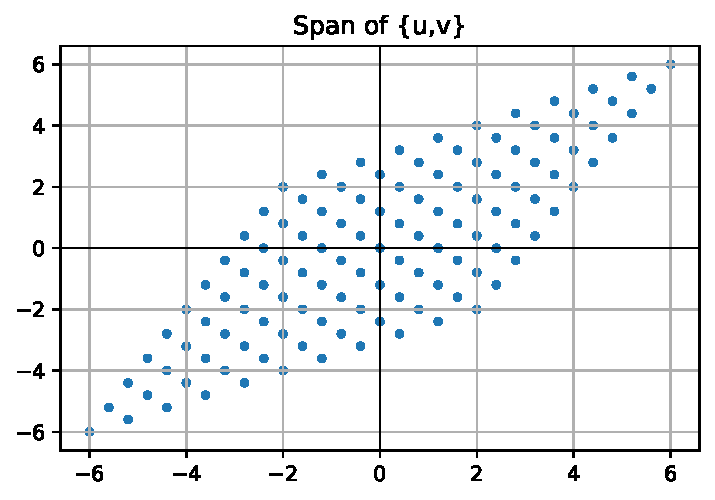
\includegraphics[keepaspectratio]{books/en-US/lab_files/figure-latex/cell-191-output-1.pdf}}

You'll see a filled grid - the entire plane, because the two vectors are
independent.

\begin{enumerate}
\def\labelenumi{\arabic{enumi}.}
\setcounter{enumi}{3}
\tightlist
\item
  Generating set of a space
\end{enumerate}

For \(\mathbb{R}^3\):

\begin{Shaded}
\begin{Highlighting}[]
\NormalTok{basis }\OperatorTok{=}\NormalTok{ [Matrix([}\DecValTok{1}\NormalTok{,}\DecValTok{0}\NormalTok{,}\DecValTok{0}\NormalTok{]), Matrix([}\DecValTok{0}\NormalTok{,}\DecValTok{1}\NormalTok{,}\DecValTok{0}\NormalTok{]), Matrix([}\DecValTok{0}\NormalTok{,}\DecValTok{0}\NormalTok{,}\DecValTok{1}\NormalTok{])]}
\NormalTok{M }\OperatorTok{=}\NormalTok{ Matrix.hstack(}\OperatorTok{*}\NormalTok{basis)}
\BuiltInTok{print}\NormalTok{(}\StringTok{"Rank:"}\NormalTok{, M.rank())}
\end{Highlighting}
\end{Shaded}

\begin{verbatim}
Rank: 3
\end{verbatim}

Rank = 3 → this set spans the whole space.

\begin{enumerate}
\def\labelenumi{\arabic{enumi}.}
\setcounter{enumi}{4}
\tightlist
\item
  Testing if a vector is in the span
\end{enumerate}

Example: Is \([3,5]\) in the span of \([1,2]\) and \([2,1]\)?

\begin{Shaded}
\begin{Highlighting}[]
\NormalTok{u }\OperatorTok{=}\NormalTok{ Matrix([}\DecValTok{1}\NormalTok{,}\DecValTok{2}\NormalTok{])}
\NormalTok{v }\OperatorTok{=}\NormalTok{ Matrix([}\DecValTok{2}\NormalTok{,}\DecValTok{1}\NormalTok{])}
\NormalTok{target }\OperatorTok{=}\NormalTok{ Matrix([}\DecValTok{3}\NormalTok{,}\DecValTok{5}\NormalTok{])}

\NormalTok{M }\OperatorTok{=}\NormalTok{ Matrix.hstack(u,v)}
\NormalTok{solution }\OperatorTok{=}\NormalTok{ M.gauss\_jordan\_solve(target)}
\BuiltInTok{print}\NormalTok{(}\StringTok{"Coefficients (a,b):"}\NormalTok{, solution)}
\end{Highlighting}
\end{Shaded}

\begin{verbatim}
Coefficients (a,b): (Matrix([
[7/3],
[1/3]]), Matrix(0, 1, []))
\end{verbatim}

If a solution exists, the target is in the span.

\subsubsection{Try It Yourself}\label{try-it-yourself-131}

\begin{enumerate}
\def\labelenumi{\arabic{enumi}.}
\tightlist
\item
  Test if \([4,6]\) is in the span of \([1,2]\).
\item
  Visualize the span of \([1,0,0]\) and \([0,1,0]\) in \(\mathbb{R}^3\).
  What does it look like?
\item
  Create a random 3×3 matrix. Use \texttt{rank()} to check if its
  columns span \(\mathbb{R}^3\).
\end{enumerate}

\subsubsection{The Takeaway}\label{the-takeaway-15}

\begin{itemize}
\tightlist
\item
  Span = all linear combinations of a set of vectors.
\item
  Independent vectors span bigger spaces; dependent ones collapse to
  smaller spaces.
\item
  Generating sets are the foundation of bases and coordinate systems.
\end{itemize}

\subsection{34. Linear Independence and Dependence (No Redundancy
vs.~Redundancy)}\label{linear-independence-and-dependence-no-redundancy-vs.-redundancy}

A set of vectors is linearly independent if none of them can be written
as a combination of the others. If at least one can, the set is
dependent. This distinction tells us whether a set of vectors has
redundancy.

\subsubsection{Set Up Your Lab}\label{set-up-your-lab-33}

\begin{Shaded}
\begin{Highlighting}[]
\ImportTok{import}\NormalTok{ numpy }\ImportTok{as}\NormalTok{ np}
\ImportTok{from}\NormalTok{ sympy }\ImportTok{import}\NormalTok{ Matrix}
\end{Highlighting}
\end{Shaded}

\subsubsection{Step-by-Step Code
Walkthrough}\label{step-by-step-code-walkthrough-33}

\begin{enumerate}
\def\labelenumi{\arabic{enumi}.}
\tightlist
\item
  Independent vectors example
\end{enumerate}

\begin{Shaded}
\begin{Highlighting}[]
\NormalTok{v1 }\OperatorTok{=}\NormalTok{ Matrix([}\DecValTok{1}\NormalTok{, }\DecValTok{0}\NormalTok{, }\DecValTok{0}\NormalTok{])}
\NormalTok{v2 }\OperatorTok{=}\NormalTok{ Matrix([}\DecValTok{0}\NormalTok{, }\DecValTok{1}\NormalTok{, }\DecValTok{0}\NormalTok{])}
\NormalTok{v3 }\OperatorTok{=}\NormalTok{ Matrix([}\DecValTok{0}\NormalTok{, }\DecValTok{0}\NormalTok{, }\DecValTok{1}\NormalTok{])}

\NormalTok{M }\OperatorTok{=}\NormalTok{ Matrix.hstack(v1, v2, v3)}
\BuiltInTok{print}\NormalTok{(}\StringTok{"Rank:"}\NormalTok{, M.rank(), }\StringTok{" Number of vectors:"}\NormalTok{, M.shape[}\DecValTok{1}\NormalTok{])}
\end{Highlighting}
\end{Shaded}

\begin{verbatim}
Rank: 3  Number of vectors: 3
\end{verbatim}

Rank = 3, number of vectors = 3 → all independent.

\begin{enumerate}
\def\labelenumi{\arabic{enumi}.}
\setcounter{enumi}{1}
\tightlist
\item
  Dependent vectors example
\end{enumerate}

\begin{Shaded}
\begin{Highlighting}[]
\NormalTok{v1 }\OperatorTok{=}\NormalTok{ Matrix([}\DecValTok{1}\NormalTok{, }\DecValTok{2}\NormalTok{, }\DecValTok{3}\NormalTok{])}
\NormalTok{v2 }\OperatorTok{=}\NormalTok{ Matrix([}\DecValTok{2}\NormalTok{, }\DecValTok{4}\NormalTok{, }\DecValTok{6}\NormalTok{])}
\NormalTok{v3 }\OperatorTok{=}\NormalTok{ Matrix([}\DecValTok{3}\NormalTok{, }\DecValTok{6}\NormalTok{, }\DecValTok{9}\NormalTok{])}

\NormalTok{M }\OperatorTok{=}\NormalTok{ Matrix.hstack(v1, v2, v3)}
\BuiltInTok{print}\NormalTok{(}\StringTok{"Rank:"}\NormalTok{, M.rank(), }\StringTok{" Number of vectors:"}\NormalTok{, M.shape[}\DecValTok{1}\NormalTok{])}
\end{Highlighting}
\end{Shaded}

\begin{verbatim}
Rank: 1  Number of vectors: 3
\end{verbatim}

Rank = 1, number of vectors = 3 → they're dependent (multiples of each
other).

\begin{enumerate}
\def\labelenumi{\arabic{enumi}.}
\setcounter{enumi}{2}
\tightlist
\item
  Checking dependence automatically
\end{enumerate}

A quick test: if rank \textless{} number of vectors → dependent.

\begin{Shaded}
\begin{Highlighting}[]
\KeywordTok{def}\NormalTok{ check\_independence(vectors):}
\NormalTok{    M }\OperatorTok{=}\NormalTok{ Matrix.hstack(}\OperatorTok{*}\NormalTok{vectors)}
    \ControlFlowTok{return}\NormalTok{ M.rank() }\OperatorTok{==}\NormalTok{ M.shape[}\DecValTok{1}\NormalTok{]}

\BuiltInTok{print}\NormalTok{(}\StringTok{"Independent?"}\NormalTok{, check\_independence([Matrix([}\DecValTok{1}\NormalTok{,}\DecValTok{0}\NormalTok{]), Matrix([}\DecValTok{0}\NormalTok{,}\DecValTok{1}\NormalTok{])]))}
\BuiltInTok{print}\NormalTok{(}\StringTok{"Independent?"}\NormalTok{, check\_independence([Matrix([}\DecValTok{1}\NormalTok{,}\DecValTok{2}\NormalTok{]), Matrix([}\DecValTok{2}\NormalTok{,}\DecValTok{4}\NormalTok{])]))}
\end{Highlighting}
\end{Shaded}

\begin{verbatim}
Independent? True
Independent? False
\end{verbatim}

\begin{enumerate}
\def\labelenumi{\arabic{enumi}.}
\setcounter{enumi}{3}
\tightlist
\item
  Solving for dependence relation
\end{enumerate}

If vectors are dependent, we can find coefficients \(c_1, c_2, …\) such
that

\[
c_1 v_1 + c_2 v_2 + … + c_k v_k = 0
\]

with some \(c_i \neq 0\).

\begin{Shaded}
\begin{Highlighting}[]
\NormalTok{M }\OperatorTok{=}\NormalTok{ Matrix.hstack(Matrix([}\DecValTok{1}\NormalTok{,}\DecValTok{2}\NormalTok{]), Matrix([}\DecValTok{2}\NormalTok{,}\DecValTok{4}\NormalTok{]))}
\NormalTok{null\_space }\OperatorTok{=}\NormalTok{ M.nullspace()}
\BuiltInTok{print}\NormalTok{(}\StringTok{"Dependence relation (coefficients):"}\NormalTok{, null\_space)}
\end{Highlighting}
\end{Shaded}

\begin{verbatim}
Dependence relation (coefficients): [Matrix([
[-2],
[ 1]])]
\end{verbatim}

This shows the exact linear relation.

\begin{enumerate}
\def\labelenumi{\arabic{enumi}.}
\setcounter{enumi}{4}
\tightlist
\item
  Random example
\end{enumerate}

\begin{Shaded}
\begin{Highlighting}[]
\NormalTok{np.random.seed(}\DecValTok{0}\NormalTok{)}
\NormalTok{R }\OperatorTok{=}\NormalTok{ Matrix(np.random.randint(}\OperatorTok{{-}}\DecValTok{3}\NormalTok{, }\DecValTok{4}\NormalTok{, (}\DecValTok{3}\NormalTok{,}\DecValTok{3}\NormalTok{)))}
\BuiltInTok{print}\NormalTok{(}\StringTok{"Random matrix:}\CharTok{\textbackslash{}n}\StringTok{"}\NormalTok{, R)}
\BuiltInTok{print}\NormalTok{(}\StringTok{"Rank:"}\NormalTok{, R.rank())}
\end{Highlighting}
\end{Shaded}

\begin{verbatim}
Random matrix:
 Matrix([[1, 2, -3], [0, 0, 0], [-2, 0, 2]])
Rank: 2
\end{verbatim}

Depending on the rank, the columns may be independent (rank = 3) or
dependent (rank \textless{} 3).

\subsubsection{Try It Yourself}\label{try-it-yourself-132}

\begin{enumerate}
\def\labelenumi{\arabic{enumi}.}
\tightlist
\item
  Test if \([1,1,0], [0,1,1], [1,2,1]\) are independent.
\item
  Generate 4 random vectors in \(\mathbb{R}^3\). Can they ever be
  independent? Why or why not?
\item
  Find the dependence relation for \([2,4], [3,6]\).
\end{enumerate}

\subsubsection{The Takeaway}\label{the-takeaway-16}

\begin{itemize}
\tightlist
\item
  Independent set: no redundancy, each vector adds a new direction.
\item
  Dependent set: at least one vector is unnecessary (it lies in the span
  of others).
\item
  Independence is the key to defining basis and dimension.
\end{itemize}

\subsection{35. Basis and Coordinates (Naming Every Vector
Uniquely)}\label{basis-and-coordinates-naming-every-vector-uniquely}

A basis is a set of independent vectors that span a space. It's like
choosing a coordinate system: every vector in the space can be expressed
uniquely as a combination of basis vectors. In this lab, we'll see how
to find bases and compute coordinates relative to them.

\subsubsection{Set Up Your Lab}\label{set-up-your-lab-34}

\begin{Shaded}
\begin{Highlighting}[]
\ImportTok{import}\NormalTok{ numpy }\ImportTok{as}\NormalTok{ np}
\ImportTok{from}\NormalTok{ sympy }\ImportTok{import}\NormalTok{ Matrix}
\end{Highlighting}
\end{Shaded}

\subsubsection{Step-by-Step Code
Walkthrough}\label{step-by-step-code-walkthrough-34}

\begin{enumerate}
\def\labelenumi{\arabic{enumi}.}
\tightlist
\item
  Standard basis in \(\mathbb{R}^3\)
\end{enumerate}

\begin{Shaded}
\begin{Highlighting}[]
\NormalTok{e1 }\OperatorTok{=}\NormalTok{ Matrix([}\DecValTok{1}\NormalTok{,}\DecValTok{0}\NormalTok{,}\DecValTok{0}\NormalTok{])}
\NormalTok{e2 }\OperatorTok{=}\NormalTok{ Matrix([}\DecValTok{0}\NormalTok{,}\DecValTok{1}\NormalTok{,}\DecValTok{0}\NormalTok{])}
\NormalTok{e3 }\OperatorTok{=}\NormalTok{ Matrix([}\DecValTok{0}\NormalTok{,}\DecValTok{0}\NormalTok{,}\DecValTok{1}\NormalTok{])}

\NormalTok{M }\OperatorTok{=}\NormalTok{ Matrix.hstack(e1, e2, e3)}
\BuiltInTok{print}\NormalTok{(}\StringTok{"Rank:"}\NormalTok{, M.rank())}
\end{Highlighting}
\end{Shaded}

\begin{verbatim}
Rank: 3
\end{verbatim}

These three independent vectors form the standard basis of
\(\mathbb{R}^3\). Any vector like \([2,5,-1]\) can be expressed as

\[
2e_1 + 5e_2 - 1e_3
\]

\begin{enumerate}
\def\labelenumi{\arabic{enumi}.}
\setcounter{enumi}{1}
\tightlist
\item
  Finding a basis from dependent vectors
\end{enumerate}

\begin{Shaded}
\begin{Highlighting}[]
\NormalTok{v1 }\OperatorTok{=}\NormalTok{ Matrix([}\DecValTok{1}\NormalTok{,}\DecValTok{2}\NormalTok{,}\DecValTok{3}\NormalTok{])}
\NormalTok{v2 }\OperatorTok{=}\NormalTok{ Matrix([}\DecValTok{2}\NormalTok{,}\DecValTok{4}\NormalTok{,}\DecValTok{6}\NormalTok{])}
\NormalTok{v3 }\OperatorTok{=}\NormalTok{ Matrix([}\DecValTok{1}\NormalTok{,}\DecValTok{0}\NormalTok{,}\DecValTok{1}\NormalTok{])}

\NormalTok{M }\OperatorTok{=}\NormalTok{ Matrix.hstack(v1,v2,v3)}
\BuiltInTok{print}\NormalTok{(}\StringTok{"Column space basis:"}\NormalTok{, M.columnspace())}
\end{Highlighting}
\end{Shaded}

\begin{verbatim}
Column space basis: [Matrix([
[1],
[2],
[3]]), Matrix([
[1],
[0],
[1]])]
\end{verbatim}

SymPy extracts independent columns automatically. This gives a basis for
the column space.

\begin{enumerate}
\def\labelenumi{\arabic{enumi}.}
\setcounter{enumi}{2}
\tightlist
\item
  Coordinates relative to a basis
\end{enumerate}

Suppose basis = \(\{ [1,0], [1,1] \}\). Express vector \([3,5]\) in this
basis.

\begin{Shaded}
\begin{Highlighting}[]
\NormalTok{B }\OperatorTok{=}\NormalTok{ Matrix.hstack(Matrix([}\DecValTok{1}\NormalTok{,}\DecValTok{0}\NormalTok{]), Matrix([}\DecValTok{1}\NormalTok{,}\DecValTok{1}\NormalTok{]))}
\NormalTok{target }\OperatorTok{=}\NormalTok{ Matrix([}\DecValTok{3}\NormalTok{,}\DecValTok{5}\NormalTok{])}

\NormalTok{coords }\OperatorTok{=}\NormalTok{ B.solve\_least\_squares(target)}
\BuiltInTok{print}\NormalTok{(}\StringTok{"Coordinates in basis B:"}\NormalTok{, coords)}
\end{Highlighting}
\end{Shaded}

\begin{verbatim}
Coordinates in basis B: Matrix([[-2], [5]])
\end{verbatim}

So \([3,5] = 3·[1,0] + 2·[1,1]\).

\begin{enumerate}
\def\labelenumi{\arabic{enumi}.}
\setcounter{enumi}{3}
\tightlist
\item
  Basis change
\end{enumerate}

If we switch to a different basis, coordinates change but the vector
stays the same.

\begin{Shaded}
\begin{Highlighting}[]
\NormalTok{new\_basis }\OperatorTok{=}\NormalTok{ Matrix.hstack(Matrix([}\DecValTok{2}\NormalTok{,}\DecValTok{1}\NormalTok{]), Matrix([}\DecValTok{1}\NormalTok{,}\DecValTok{2}\NormalTok{]))}
\NormalTok{coords\_new }\OperatorTok{=}\NormalTok{ new\_basis.solve\_least\_squares(target)}
\BuiltInTok{print}\NormalTok{(}\StringTok{"Coordinates in new basis:"}\NormalTok{, coords\_new)}
\end{Highlighting}
\end{Shaded}

\begin{verbatim}
Coordinates in new basis: Matrix([[1/3], [7/3]])
\end{verbatim}

\begin{enumerate}
\def\labelenumi{\arabic{enumi}.}
\setcounter{enumi}{4}
\tightlist
\item
  Random example
\end{enumerate}

Generate 3 random vectors in \(\mathbb{R}^3\). Check if they form a
basis.

\begin{Shaded}
\begin{Highlighting}[]
\NormalTok{np.random.seed(}\DecValTok{1}\NormalTok{)}
\NormalTok{R }\OperatorTok{=}\NormalTok{ Matrix(np.random.randint(}\OperatorTok{{-}}\DecValTok{3}\NormalTok{,}\DecValTok{4}\NormalTok{,(}\DecValTok{3}\NormalTok{,}\DecValTok{3}\NormalTok{)))}
\BuiltInTok{print}\NormalTok{(}\StringTok{"Random matrix:}\CharTok{\textbackslash{}n}\StringTok{"}\NormalTok{, R)}
\BuiltInTok{print}\NormalTok{(}\StringTok{"Rank:"}\NormalTok{, R.rank())}
\end{Highlighting}
\end{Shaded}

\begin{verbatim}
Random matrix:
 Matrix([[2, 0, 1], [-3, -2, 0], [2, -3, -3]])
Rank: 3
\end{verbatim}

If rank = 3 → basis for \(\mathbb{R}^3\). Otherwise, only span a
subspace.

\subsubsection{Try It Yourself}\label{try-it-yourself-133}

\begin{enumerate}
\def\labelenumi{\arabic{enumi}.}
\tightlist
\item
  Check if \([1,2], [3,4]\) form a basis of \(\mathbb{R}^2\).
\item
  Express vector \([7,5]\) in that basis.
\item
  Create 4 random vectors in \(\mathbb{R}^3\). Find a basis for their
  span.
\end{enumerate}

\subsubsection{The Takeaway}\label{the-takeaway-17}

\begin{itemize}
\tightlist
\item
  A basis = minimal set of vectors that span a space.
\item
  Every vector has a unique coordinate representation in a given basis.
\item
  Changing bases changes the coordinates, not the vector itself.
\end{itemize}

\subsection{36. Dimension (How Many
Directions)}\label{dimension-how-many-directions}

The dimension of a vector space is the number of independent directions
it has. Formally, it's the number of vectors in any basis of the space.
Dimension tells us the ``size'' of a space in terms of degrees of
freedom.

\subsubsection{Set Up Your Lab}\label{set-up-your-lab-35}

\begin{Shaded}
\begin{Highlighting}[]
\ImportTok{import}\NormalTok{ numpy }\ImportTok{as}\NormalTok{ np}
\ImportTok{from}\NormalTok{ sympy }\ImportTok{import}\NormalTok{ Matrix}
\end{Highlighting}
\end{Shaded}

\subsubsection{Step-by-Step Code
Walkthrough}\label{step-by-step-code-walkthrough-35}

\begin{enumerate}
\def\labelenumi{\arabic{enumi}.}
\tightlist
\item
  Dimension of \(\mathbb{R}^n\)
\end{enumerate}

The dimension of \(\mathbb{R}^n\) is \(n\).

\begin{Shaded}
\begin{Highlighting}[]
\NormalTok{n }\OperatorTok{=} \DecValTok{4}
\NormalTok{basis }\OperatorTok{=}\NormalTok{ [Matrix.eye(n)[:,i] }\ControlFlowTok{for}\NormalTok{ i }\KeywordTok{in} \BuiltInTok{range}\NormalTok{(n)]}
\BuiltInTok{print}\NormalTok{(}\StringTok{"Basis for R\^{}4:"}\NormalTok{, basis)}
\BuiltInTok{print}\NormalTok{(}\StringTok{"Dimension of R\^{}4:"}\NormalTok{, }\BuiltInTok{len}\NormalTok{(basis))}
\end{Highlighting}
\end{Shaded}

\begin{verbatim}
Basis for R^4: [Matrix([
[1],
[0],
[0],
[0]]), Matrix([
[0],
[1],
[0],
[0]]), Matrix([
[0],
[0],
[1],
[0]]), Matrix([
[0],
[0],
[0],
[1]])]
Dimension of R^4: 4
\end{verbatim}

Each standard unit vector adds one independent direction → dimension =
4.

\begin{enumerate}
\def\labelenumi{\arabic{enumi}.}
\setcounter{enumi}{1}
\tightlist
\item
  Dimension via rank
\end{enumerate}

The rank of a matrix equals the dimension of its column space.

\begin{Shaded}
\begin{Highlighting}[]
\NormalTok{A }\OperatorTok{=}\NormalTok{ Matrix([}
\NormalTok{    [}\DecValTok{1}\NormalTok{,}\DecValTok{2}\NormalTok{,}\DecValTok{3}\NormalTok{],}
\NormalTok{    [}\DecValTok{2}\NormalTok{,}\DecValTok{4}\NormalTok{,}\DecValTok{6}\NormalTok{],}
\NormalTok{    [}\DecValTok{1}\NormalTok{,}\DecValTok{0}\NormalTok{,}\DecValTok{1}\NormalTok{]}
\NormalTok{])}

\BuiltInTok{print}\NormalTok{(}\StringTok{"Rank (dimension of column space):"}\NormalTok{, A.rank())}
\end{Highlighting}
\end{Shaded}

\begin{verbatim}
Rank (dimension of column space): 2
\end{verbatim}

Here, rank = 2 → the column space is a 2D plane inside \(\mathbb{R}^3\).

\begin{enumerate}
\def\labelenumi{\arabic{enumi}.}
\setcounter{enumi}{2}
\tightlist
\item
  Null space dimension
\end{enumerate}

The null space dimension is given by:

\[
\text{dim(Null(A))} = \#\text{variables} - \text{rank(A)}
\]

\begin{Shaded}
\begin{Highlighting}[]
\BuiltInTok{print}\NormalTok{(}\StringTok{"Null space basis:"}\NormalTok{, A.nullspace())}
\BuiltInTok{print}\NormalTok{(}\StringTok{"Dimension of null space:"}\NormalTok{, }\BuiltInTok{len}\NormalTok{(A.nullspace()))}
\end{Highlighting}
\end{Shaded}

\begin{verbatim}
Null space basis: [Matrix([
[-1],
[-1],
[ 1]])]
Dimension of null space: 1
\end{verbatim}

This is the number of free variables in a solution.

\begin{enumerate}
\def\labelenumi{\arabic{enumi}.}
\setcounter{enumi}{3}
\tightlist
\item
  Dimension in practice
\end{enumerate}

\begin{itemize}
\tightlist
\item
  A line through the origin in \(\mathbb{R}^3\) has dimension 1.
\item
  A plane through the origin has dimension 2.
\item
  The whole \(\mathbb{R}^3\) has dimension 3.
\end{itemize}

Example:

\begin{Shaded}
\begin{Highlighting}[]
\NormalTok{v1 }\OperatorTok{=}\NormalTok{ Matrix([}\DecValTok{1}\NormalTok{,}\DecValTok{2}\NormalTok{,}\DecValTok{3}\NormalTok{])}
\NormalTok{v2 }\OperatorTok{=}\NormalTok{ Matrix([}\DecValTok{2}\NormalTok{,}\DecValTok{4}\NormalTok{,}\DecValTok{6}\NormalTok{])}
\NormalTok{span }\OperatorTok{=}\NormalTok{ Matrix.hstack(v1,v2)}
\BuiltInTok{print}\NormalTok{(}\StringTok{"Dimension of span:"}\NormalTok{, span.rank())}
\end{Highlighting}
\end{Shaded}

\begin{verbatim}
Dimension of span: 1
\end{verbatim}

Result = 1 → they only generate a line.

\begin{enumerate}
\def\labelenumi{\arabic{enumi}.}
\setcounter{enumi}{4}
\tightlist
\item
  Random example
\end{enumerate}

\begin{Shaded}
\begin{Highlighting}[]
\NormalTok{np.random.seed(}\DecValTok{2}\NormalTok{)}
\NormalTok{R }\OperatorTok{=}\NormalTok{ Matrix(np.random.randint(}\OperatorTok{{-}}\DecValTok{3}\NormalTok{,}\DecValTok{4}\NormalTok{,(}\DecValTok{4}\NormalTok{,}\DecValTok{4}\NormalTok{)))}
\BuiltInTok{print}\NormalTok{(}\StringTok{"Random 4x4 matrix:}\CharTok{\textbackslash{}n}\StringTok{"}\NormalTok{, R)}
\BuiltInTok{print}\NormalTok{(}\StringTok{"Column space dimension:"}\NormalTok{, R.rank())}
\end{Highlighting}
\end{Shaded}

\begin{verbatim}
Random 4x4 matrix:
 Matrix([[-3, 2, -3, 3], [0, -1, 0, -3], [-1, -2, 0, 2], [-1, 1, 1, 1]])
Column space dimension: 4
\end{verbatim}

Rank may be 4 (full space) or smaller (collapsed).

\subsubsection{Try It Yourself}\label{try-it-yourself-134}

\begin{enumerate}
\def\labelenumi{\arabic{enumi}.}
\item
  Find the dimension of the column space of

  \[
  \begin{bmatrix}  
  1 & 1 & 1 \\  
  0 & 1 & 1 \\  
  0 & 0 & 0  
  \end{bmatrix}
  \]
\item
  Compute the dimension of the null space of a 3×3 singular matrix.
\item
  Generate a 5×3 random matrix and compute its column space dimension.
\end{enumerate}

\subsubsection{The Takeaway}\label{the-takeaway-18}

\begin{itemize}
\tightlist
\item
  Dimension = number of independent directions.
\item
  Found by counting basis vectors (or rank).
\item
  Dimensions describe lines (1D), planes (2D), and higher subspaces
  inside larger spaces.
\end{itemize}

\subsection{37. Rank--Nullity Theorem (Dimensions That Add
Up)}\label{ranknullity-theorem-dimensions-that-add-up}

The rank--nullity theorem ties together the dimension of the column
space and the null space of a matrix. It says:

\[
\text{rank}(A) + \text{nullity}(A) = \text{number of columns of } A
\]

This is a powerful consistency check in linear algebra.

\subsubsection{Set Up Your Lab}\label{set-up-your-lab-36}

\begin{Shaded}
\begin{Highlighting}[]
\ImportTok{import}\NormalTok{ numpy }\ImportTok{as}\NormalTok{ np}
\ImportTok{from}\NormalTok{ sympy }\ImportTok{import}\NormalTok{ Matrix}
\end{Highlighting}
\end{Shaded}

\subsubsection{Step-by-Step Code
Walkthrough}\label{step-by-step-code-walkthrough-36}

\begin{enumerate}
\def\labelenumi{\arabic{enumi}.}
\tightlist
\item
  Simple 3×3 example
\end{enumerate}

\begin{Shaded}
\begin{Highlighting}[]
\NormalTok{A }\OperatorTok{=}\NormalTok{ Matrix([}
\NormalTok{    [}\DecValTok{1}\NormalTok{, }\DecValTok{2}\NormalTok{, }\DecValTok{3}\NormalTok{],}
\NormalTok{    [}\DecValTok{2}\NormalTok{, }\DecValTok{4}\NormalTok{, }\DecValTok{6}\NormalTok{],}
\NormalTok{    [}\DecValTok{1}\NormalTok{, }\DecValTok{0}\NormalTok{, }\DecValTok{1}\NormalTok{]}
\NormalTok{])}

\NormalTok{rank }\OperatorTok{=}\NormalTok{ A.rank()}
\NormalTok{nullity }\OperatorTok{=} \BuiltInTok{len}\NormalTok{(A.nullspace())}
\BuiltInTok{print}\NormalTok{(}\StringTok{"Rank:"}\NormalTok{, rank)}
\BuiltInTok{print}\NormalTok{(}\StringTok{"Nullity:"}\NormalTok{, nullity)}
\BuiltInTok{print}\NormalTok{(}\StringTok{"Rank + Nullity ="}\NormalTok{, rank }\OperatorTok{+}\NormalTok{ nullity)}
\BuiltInTok{print}\NormalTok{(}\StringTok{"Number of columns ="}\NormalTok{, A.shape[}\DecValTok{1}\NormalTok{])}
\end{Highlighting}
\end{Shaded}

\begin{verbatim}
Rank: 2
Nullity: 1
Rank + Nullity = 3
Number of columns = 3
\end{verbatim}

You should see that rank + nullity = 3, the number of columns.

\begin{enumerate}
\def\labelenumi{\arabic{enumi}.}
\setcounter{enumi}{1}
\tightlist
\item
  Full-rank case
\end{enumerate}

\begin{Shaded}
\begin{Highlighting}[]
\NormalTok{B }\OperatorTok{=}\NormalTok{ Matrix([}
\NormalTok{    [}\DecValTok{1}\NormalTok{,}\DecValTok{0}\NormalTok{,}\DecValTok{0}\NormalTok{],}
\NormalTok{    [}\DecValTok{0}\NormalTok{,}\DecValTok{1}\NormalTok{,}\DecValTok{0}\NormalTok{],}
\NormalTok{    [}\DecValTok{0}\NormalTok{,}\DecValTok{0}\NormalTok{,}\DecValTok{1}\NormalTok{]}
\NormalTok{])}

\BuiltInTok{print}\NormalTok{(}\StringTok{"Rank:"}\NormalTok{, B.rank())}
\BuiltInTok{print}\NormalTok{(}\StringTok{"Nullity:"}\NormalTok{, }\BuiltInTok{len}\NormalTok{(B.nullspace()))}
\end{Highlighting}
\end{Shaded}

\begin{verbatim}
Rank: 3
Nullity: 0
\end{verbatim}

\begin{itemize}
\tightlist
\item
  Rank = 3 (all independent).
\item
  Nullity = 0 (only zero solution to \(Bx=0\)).
\item
  Rank + Nullity = 3 columns.
\end{itemize}

\begin{enumerate}
\def\labelenumi{\arabic{enumi}.}
\setcounter{enumi}{2}
\tightlist
\item
  Wide matrix (more columns than rows)
\end{enumerate}

\begin{Shaded}
\begin{Highlighting}[]
\NormalTok{C }\OperatorTok{=}\NormalTok{ Matrix([}
\NormalTok{    [}\DecValTok{1}\NormalTok{,}\DecValTok{2}\NormalTok{,}\DecValTok{3}\NormalTok{,}\DecValTok{4}\NormalTok{],}
\NormalTok{    [}\DecValTok{0}\NormalTok{,}\DecValTok{1}\NormalTok{,}\DecValTok{1}\NormalTok{,}\DecValTok{2}\NormalTok{],}
\NormalTok{    [}\DecValTok{0}\NormalTok{,}\DecValTok{0}\NormalTok{,}\DecValTok{0}\NormalTok{,}\DecValTok{0}\NormalTok{]}
\NormalTok{])}

\NormalTok{rank }\OperatorTok{=}\NormalTok{ C.rank()}
\NormalTok{nullity }\OperatorTok{=} \BuiltInTok{len}\NormalTok{(C.nullspace())}
\BuiltInTok{print}\NormalTok{(}\StringTok{"Rank:"}\NormalTok{, rank, }\StringTok{" Nullity:"}\NormalTok{, nullity, }\StringTok{" Columns:"}\NormalTok{, C.shape[}\DecValTok{1}\NormalTok{])}
\end{Highlighting}
\end{Shaded}

\begin{verbatim}
Rank: 2  Nullity: 2  Columns: 4
\end{verbatim}

Here, nullity \textgreater{} 0 because there are more variables than
independent equations.

\begin{enumerate}
\def\labelenumi{\arabic{enumi}.}
\setcounter{enumi}{3}
\tightlist
\item
  Verifying with random matrices
\end{enumerate}

\begin{Shaded}
\begin{Highlighting}[]
\NormalTok{np.random.seed(}\DecValTok{3}\NormalTok{)}
\NormalTok{R }\OperatorTok{=}\NormalTok{ Matrix(np.random.randint(}\OperatorTok{{-}}\DecValTok{3}\NormalTok{,}\DecValTok{4}\NormalTok{,(}\DecValTok{4}\NormalTok{,}\DecValTok{5}\NormalTok{)))}
\BuiltInTok{print}\NormalTok{(}\StringTok{"Random 4x5 matrix:}\CharTok{\textbackslash{}n}\StringTok{"}\NormalTok{, R)}
\BuiltInTok{print}\NormalTok{(}\StringTok{"Rank + Nullity ="}\NormalTok{, R.rank() }\OperatorTok{+} \BuiltInTok{len}\NormalTok{(R.nullspace()))}
\BuiltInTok{print}\NormalTok{(}\StringTok{"Number of columns ="}\NormalTok{, R.shape[}\DecValTok{1}\NormalTok{])}
\end{Highlighting}
\end{Shaded}

\begin{verbatim}
Random 4x5 matrix:
 Matrix([[-1, -3, -2, 0, -3], [-3, -3, 2, 2, 0], [-1, 0, -2, -2, -1], [2, 3, -3, 1, 1]])
Rank + Nullity = 5
Number of columns = 5
\end{verbatim}

Always consistent: rank + nullity = number of columns.

\begin{enumerate}
\def\labelenumi{\arabic{enumi}.}
\setcounter{enumi}{4}
\tightlist
\item
  Geometric interpretation
\end{enumerate}

For an \(m \times n\) matrix:

\begin{itemize}
\tightlist
\item
  Rank(A) = dimension of outputs (column space).
\item
  Nullity(A) = dimension of hidden directions that collapse to 0.
\item
  Together, they use up all the ``input dimensions'' (n).
\end{itemize}

\subsubsection{Try It Yourself}\label{try-it-yourself-135}

\begin{enumerate}
\def\labelenumi{\arabic{enumi}.}
\item
  Compute rank and nullity of

  \[
  \begin{bmatrix}  
  1 & 1 & 1 \\  
  0 & 1 & 1  
  \end{bmatrix}
  \]

  Check the theorem.
\item
  Create a 2×4 random integer matrix. Confirm that rank + nullity = 4.
\item
  Explain why a tall full-rank \(5 \times 3\) matrix must have nullity =
  0.
\end{enumerate}

\subsubsection{The Takeaway}\label{the-takeaway-19}

\begin{itemize}
\tightlist
\item
  Rank + Nullity = number of columns (always true).
\item
  Rank measures independent outputs; nullity measures hidden freedom.
\item
  This theorem connects solutions of \(Ax=0\) with the structure of
  \(A\).
\end{itemize}

\subsection{38. Coordinates Relative to a Basis (Changing the
``Ruler'')}\label{coordinates-relative-to-a-basis-changing-the-ruler}

Once we choose a basis, every vector can be described with coordinates
relative to that basis. This is like changing the ``ruler'' we use to
measure vectors. In this lab, we'll practice computing coordinates in
different bases.

\subsubsection{Set Up Your Lab}\label{set-up-your-lab-37}

\begin{Shaded}
\begin{Highlighting}[]
\ImportTok{import}\NormalTok{ numpy }\ImportTok{as}\NormalTok{ np}
\ImportTok{from}\NormalTok{ sympy }\ImportTok{import}\NormalTok{ Matrix}
\end{Highlighting}
\end{Shaded}

\subsubsection{Step-by-Step Code
Walkthrough}\label{step-by-step-code-walkthrough-37}

\begin{enumerate}
\def\labelenumi{\arabic{enumi}.}
\tightlist
\item
  Standard basis coordinates
\end{enumerate}

Vector \(v = [4,5]\) in \(\mathbb{R}^2\):

\begin{Shaded}
\begin{Highlighting}[]
\NormalTok{v }\OperatorTok{=}\NormalTok{ Matrix([}\DecValTok{4}\NormalTok{,}\DecValTok{5}\NormalTok{])}
\NormalTok{e1 }\OperatorTok{=}\NormalTok{ Matrix([}\DecValTok{1}\NormalTok{,}\DecValTok{0}\NormalTok{])}
\NormalTok{e2 }\OperatorTok{=}\NormalTok{ Matrix([}\DecValTok{0}\NormalTok{,}\DecValTok{1}\NormalTok{])}

\NormalTok{B }\OperatorTok{=}\NormalTok{ Matrix.hstack(e1,e2)}
\NormalTok{coords }\OperatorTok{=}\NormalTok{ B.solve\_least\_squares(v)}
\BuiltInTok{print}\NormalTok{(}\StringTok{"Coordinates in standard basis:"}\NormalTok{, coords)}
\end{Highlighting}
\end{Shaded}

\begin{verbatim}
Coordinates in standard basis: Matrix([[4], [5]])
\end{verbatim}

Result is just \([4,5]\). Easy - the standard basis matches the
components directly.

\begin{enumerate}
\def\labelenumi{\arabic{enumi}.}
\setcounter{enumi}{1}
\tightlist
\item
  Non-standard basis
\end{enumerate}

Suppose basis = \(\{ [1,1], [1,-1] \}\). Express \(v = [4,5]\) in this
basis.

\begin{Shaded}
\begin{Highlighting}[]
\NormalTok{B2 }\OperatorTok{=}\NormalTok{ Matrix.hstack(Matrix([}\DecValTok{1}\NormalTok{,}\DecValTok{1}\NormalTok{]), Matrix([}\DecValTok{1}\NormalTok{,}\OperatorTok{{-}}\DecValTok{1}\NormalTok{]))}
\NormalTok{coords2 }\OperatorTok{=}\NormalTok{ B2.solve\_least\_squares(v)}
\BuiltInTok{print}\NormalTok{(}\StringTok{"Coordinates in new basis:"}\NormalTok{, coords2)}
\end{Highlighting}
\end{Shaded}

\begin{verbatim}
Coordinates in new basis: Matrix([[9/2], [-1/2]])
\end{verbatim}

Now \(v\) has different coordinates.

\begin{enumerate}
\def\labelenumi{\arabic{enumi}.}
\setcounter{enumi}{2}
\tightlist
\item
  Changing coordinates back
\end{enumerate}

To reconstruct the vector from coordinates:

\begin{Shaded}
\begin{Highlighting}[]
\NormalTok{reconstructed }\OperatorTok{=}\NormalTok{ B2 }\OperatorTok{*}\NormalTok{ coords2}
\BuiltInTok{print}\NormalTok{(}\StringTok{"Reconstructed vector:"}\NormalTok{, reconstructed)}
\end{Highlighting}
\end{Shaded}

\begin{verbatim}
Reconstructed vector: Matrix([[4], [5]])
\end{verbatim}

It matches the original \([4,5]\).

\begin{enumerate}
\def\labelenumi{\arabic{enumi}.}
\setcounter{enumi}{3}
\tightlist
\item
  Random basis in \(\mathbb{R}^3\)
\end{enumerate}

\begin{Shaded}
\begin{Highlighting}[]
\NormalTok{basis }\OperatorTok{=}\NormalTok{ Matrix.hstack(}
\NormalTok{    Matrix([}\DecValTok{1}\NormalTok{,}\DecValTok{0}\NormalTok{,}\DecValTok{1}\NormalTok{]),}
\NormalTok{    Matrix([}\DecValTok{0}\NormalTok{,}\DecValTok{1}\NormalTok{,}\DecValTok{1}\NormalTok{]),}
\NormalTok{    Matrix([}\DecValTok{1}\NormalTok{,}\DecValTok{1}\NormalTok{,}\DecValTok{0}\NormalTok{])}
\NormalTok{)}
\NormalTok{v }\OperatorTok{=}\NormalTok{ Matrix([}\DecValTok{2}\NormalTok{,}\DecValTok{3}\NormalTok{,}\DecValTok{4}\NormalTok{])}

\NormalTok{coords }\OperatorTok{=}\NormalTok{ basis.solve\_least\_squares(v)}
\BuiltInTok{print}\NormalTok{(}\StringTok{"Coordinates of v in random basis:"}\NormalTok{, coords)}
\end{Highlighting}
\end{Shaded}

\begin{verbatim}
Coordinates of v in random basis: Matrix([[3/2], [5/2], [1/2]])
\end{verbatim}

Any independent set of 3 vectors in \(\mathbb{R}^3\) works as a basis.

\begin{enumerate}
\def\labelenumi{\arabic{enumi}.}
\setcounter{enumi}{4}
\tightlist
\item
  Visualization in 2D
\end{enumerate}

Let's compare coordinates in two bases.

\begin{Shaded}
\begin{Highlighting}[]
\ImportTok{import}\NormalTok{ matplotlib.pyplot }\ImportTok{as}\NormalTok{ plt}

\NormalTok{v }\OperatorTok{=}\NormalTok{ np.array([}\DecValTok{4}\NormalTok{,}\DecValTok{5}\NormalTok{])}
\NormalTok{b1 }\OperatorTok{=}\NormalTok{ np.array([}\DecValTok{1}\NormalTok{,}\DecValTok{1}\NormalTok{])}
\NormalTok{b2 }\OperatorTok{=}\NormalTok{ np.array([}\DecValTok{1}\NormalTok{,}\OperatorTok{{-}}\DecValTok{1}\NormalTok{])}

\NormalTok{plt.quiver(}\DecValTok{0}\NormalTok{,}\DecValTok{0}\NormalTok{,v[}\DecValTok{0}\NormalTok{],v[}\DecValTok{1}\NormalTok{],angles}\OperatorTok{=}\StringTok{\textquotesingle{}xy\textquotesingle{}}\NormalTok{,scale\_units}\OperatorTok{=}\StringTok{\textquotesingle{}xy\textquotesingle{}}\NormalTok{,scale}\OperatorTok{=}\DecValTok{1}\NormalTok{,color}\OperatorTok{=}\StringTok{\textquotesingle{}blue\textquotesingle{}}\NormalTok{,label}\OperatorTok{=}\StringTok{\textquotesingle{}v\textquotesingle{}}\NormalTok{)}
\NormalTok{plt.quiver(}\DecValTok{0}\NormalTok{,}\DecValTok{0}\NormalTok{,b1[}\DecValTok{0}\NormalTok{],b1[}\DecValTok{1}\NormalTok{],angles}\OperatorTok{=}\StringTok{\textquotesingle{}xy\textquotesingle{}}\NormalTok{,scale\_units}\OperatorTok{=}\StringTok{\textquotesingle{}xy\textquotesingle{}}\NormalTok{,scale}\OperatorTok{=}\DecValTok{1}\NormalTok{,color}\OperatorTok{=}\StringTok{\textquotesingle{}red\textquotesingle{}}\NormalTok{,label}\OperatorTok{=}\StringTok{\textquotesingle{}basis1\textquotesingle{}}\NormalTok{)}
\NormalTok{plt.quiver(}\DecValTok{0}\NormalTok{,}\DecValTok{0}\NormalTok{,b2[}\DecValTok{0}\NormalTok{],b2[}\DecValTok{1}\NormalTok{],angles}\OperatorTok{=}\StringTok{\textquotesingle{}xy\textquotesingle{}}\NormalTok{,scale\_units}\OperatorTok{=}\StringTok{\textquotesingle{}xy\textquotesingle{}}\NormalTok{,scale}\OperatorTok{=}\DecValTok{1}\NormalTok{,color}\OperatorTok{=}\StringTok{\textquotesingle{}green\textquotesingle{}}\NormalTok{,label}\OperatorTok{=}\StringTok{\textquotesingle{}basis2\textquotesingle{}}\NormalTok{)}

\NormalTok{plt.xlim(}\OperatorTok{{-}}\DecValTok{1}\NormalTok{,}\DecValTok{6}\NormalTok{)}
\NormalTok{plt.ylim(}\OperatorTok{{-}}\DecValTok{6}\NormalTok{,}\DecValTok{6}\NormalTok{)}
\NormalTok{plt.legend()}
\NormalTok{plt.grid()}
\NormalTok{plt.show()}
\end{Highlighting}
\end{Shaded}

\pandocbounded{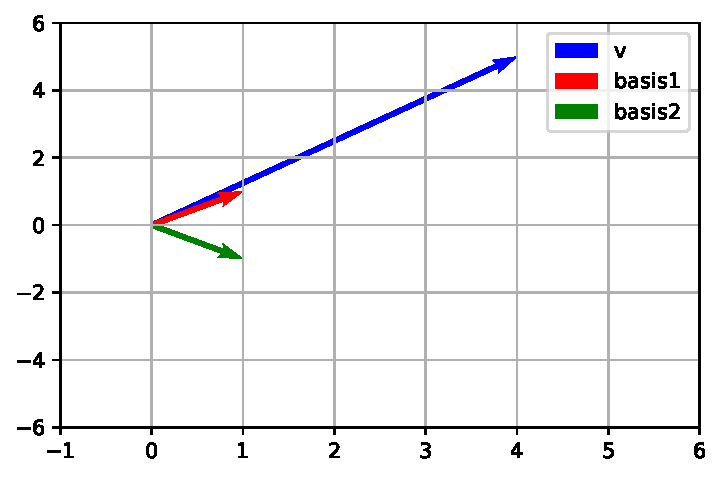
\includegraphics[keepaspectratio]{books/en-US/lab_files/figure-latex/cell-222-output-1.pdf}}

Even though the basis vectors look different, they span the same space,
and \(v\) can be expressed in terms of them.

\subsubsection{Try It Yourself}\label{try-it-yourself-136}

\begin{enumerate}
\def\labelenumi{\arabic{enumi}.}
\tightlist
\item
  Express \([7,3]\) in the basis \(\{[2,0], [0,3]\}\).
\item
  Pick three independent random vectors in \(\mathbb{R}^3\). Write down
  the coordinates of \([1,2,3]\) in that basis.
\item
  Verify that reconstructing always gives the original vector.
\end{enumerate}

\subsubsection{The Takeaway}\label{the-takeaway-20}

\begin{itemize}
\tightlist
\item
  A basis provides a coordinate system for vectors.
\item
  Coordinates depend on the basis, but the underlying vector doesn't
  change.
\item
  Changing the basis is like changing the ``ruler'' you measure vectors
  with.
\end{itemize}

\subsection{39. Change-of-Basis Matrices (Moving Between Coordinate
Systems)}\label{change-of-basis-matrices-moving-between-coordinate-systems}

When we switch from one basis to another, we need a change-of-basis
matrix. This matrix acts like a translator: it converts coordinates in
one system to coordinates in another.

\subsubsection{Set Up Your Lab}\label{set-up-your-lab-38}

\begin{Shaded}
\begin{Highlighting}[]
\ImportTok{import}\NormalTok{ numpy }\ImportTok{as}\NormalTok{ np}
\ImportTok{from}\NormalTok{ sympy }\ImportTok{import}\NormalTok{ Matrix}
\end{Highlighting}
\end{Shaded}

\subsubsection{Step-by-Step Code
Walkthrough}\label{step-by-step-code-walkthrough-38}

\begin{enumerate}
\def\labelenumi{\arabic{enumi}.}
\tightlist
\item
  Two bases in \(\mathbb{R}^2\)
\end{enumerate}

Let's define:

\begin{itemize}
\tightlist
\item
  Basis \(B = \{ [1,0], [0,1] \}\) (standard basis).
\item
  Basis \(C = \{ [1,1], [1,-1] \}\).
\end{itemize}

\begin{Shaded}
\begin{Highlighting}[]
\NormalTok{B }\OperatorTok{=}\NormalTok{ Matrix.hstack(Matrix([}\DecValTok{1}\NormalTok{,}\DecValTok{0}\NormalTok{]), Matrix([}\DecValTok{0}\NormalTok{,}\DecValTok{1}\NormalTok{]))}
\NormalTok{C }\OperatorTok{=}\NormalTok{ Matrix.hstack(Matrix([}\DecValTok{1}\NormalTok{,}\DecValTok{1}\NormalTok{]), Matrix([}\DecValTok{1}\NormalTok{,}\OperatorTok{{-}}\DecValTok{1}\NormalTok{]))}
\end{Highlighting}
\end{Shaded}

\begin{enumerate}
\def\labelenumi{\arabic{enumi}.}
\setcounter{enumi}{1}
\tightlist
\item
  Change-of-basis matrix
\end{enumerate}

The matrix that converts C-coordinates → standard coordinates is just
\(C\).

\begin{Shaded}
\begin{Highlighting}[]
\BuiltInTok{print}\NormalTok{(}\StringTok{"C (basis matrix):}\CharTok{\textbackslash{}n}\StringTok{"}\NormalTok{, C)}
\end{Highlighting}
\end{Shaded}

\begin{verbatim}
C (basis matrix):
 Matrix([[1, 1], [1, -1]])
\end{verbatim}

To go the other way (standard → C), we compute the inverse of \(C\).

\begin{Shaded}
\begin{Highlighting}[]
\NormalTok{C\_inv }\OperatorTok{=}\NormalTok{ C.inv()}
\BuiltInTok{print}\NormalTok{(}\StringTok{"C inverse:}\CharTok{\textbackslash{}n}\StringTok{"}\NormalTok{, C\_inv)}
\end{Highlighting}
\end{Shaded}

\begin{verbatim}
C inverse:
 Matrix([[1/2, 1/2], [1/2, -1/2]])
\end{verbatim}

\begin{enumerate}
\def\labelenumi{\arabic{enumi}.}
\setcounter{enumi}{2}
\tightlist
\item
  Converting coordinates
\end{enumerate}

Vector \(v = [4,5]\).

\begin{itemize}
\tightlist
\item
  In standard basis:
\end{itemize}

\begin{Shaded}
\begin{Highlighting}[]
\NormalTok{v }\OperatorTok{=}\NormalTok{ Matrix([}\DecValTok{4}\NormalTok{,}\DecValTok{5}\NormalTok{])}
\NormalTok{coords\_in\_standard }\OperatorTok{=}\NormalTok{ v}
\BuiltInTok{print}\NormalTok{(}\StringTok{"Coordinates in standard basis:"}\NormalTok{, coords\_in\_standard)}
\end{Highlighting}
\end{Shaded}

\begin{verbatim}
Coordinates in standard basis: Matrix([[4], [5]])
\end{verbatim}

\begin{itemize}
\tightlist
\item
  In basis \(C\):
\end{itemize}

\begin{Shaded}
\begin{Highlighting}[]
\NormalTok{coords\_in\_C }\OperatorTok{=}\NormalTok{ C\_inv }\OperatorTok{*}\NormalTok{ v}
\BuiltInTok{print}\NormalTok{(}\StringTok{"Coordinates in C basis:"}\NormalTok{, coords\_in\_C)}
\end{Highlighting}
\end{Shaded}

\begin{verbatim}
Coordinates in C basis: Matrix([[9/2], [-1/2]])
\end{verbatim}

\begin{itemize}
\tightlist
\item
  Convert back:
\end{itemize}

\begin{Shaded}
\begin{Highlighting}[]
\NormalTok{reconstructed }\OperatorTok{=}\NormalTok{ C }\OperatorTok{*}\NormalTok{ coords\_in\_C}
\BuiltInTok{print}\NormalTok{(}\StringTok{"Reconstructed vector:"}\NormalTok{, reconstructed)}
\end{Highlighting}
\end{Shaded}

\begin{verbatim}
Reconstructed vector: Matrix([[4], [5]])
\end{verbatim}

The reconstruction matches the original vector.

\begin{enumerate}
\def\labelenumi{\arabic{enumi}.}
\setcounter{enumi}{3}
\tightlist
\item
  General formula
\end{enumerate}

If \(P\) is the change-of-basis matrix from basis \(B\) to basis \(C\):

\[
[v]_C = P^{-1}[v]_B
\]

\[
[v]_B = P[v]_C
\]

Here, \(P\) is the matrix of new basis vectors written in terms of the
old basis.

\begin{enumerate}
\def\labelenumi{\arabic{enumi}.}
\setcounter{enumi}{4}
\tightlist
\item
  Random 3D example
\end{enumerate}

\begin{Shaded}
\begin{Highlighting}[]
\NormalTok{B }\OperatorTok{=}\NormalTok{ Matrix.eye(}\DecValTok{3}\NormalTok{)  }\CommentTok{\# standard basis}
\NormalTok{C }\OperatorTok{=}\NormalTok{ Matrix.hstack(}
\NormalTok{    Matrix([}\DecValTok{1}\NormalTok{,}\DecValTok{0}\NormalTok{,}\DecValTok{1}\NormalTok{]),}
\NormalTok{    Matrix([}\DecValTok{0}\NormalTok{,}\DecValTok{1}\NormalTok{,}\DecValTok{1}\NormalTok{]),}
\NormalTok{    Matrix([}\DecValTok{1}\NormalTok{,}\DecValTok{1}\NormalTok{,}\DecValTok{0}\NormalTok{])}
\NormalTok{)}

\NormalTok{v }\OperatorTok{=}\NormalTok{ Matrix([}\DecValTok{2}\NormalTok{,}\DecValTok{3}\NormalTok{,}\DecValTok{4}\NormalTok{])}

\NormalTok{C\_inv }\OperatorTok{=}\NormalTok{ C.inv()}
\NormalTok{coords\_in\_C }\OperatorTok{=}\NormalTok{ C\_inv }\OperatorTok{*}\NormalTok{ v}
\BuiltInTok{print}\NormalTok{(}\StringTok{"Coordinates in new basis C:"}\NormalTok{, coords\_in\_C)}

\BuiltInTok{print}\NormalTok{(}\StringTok{"Back to standard:"}\NormalTok{, C }\OperatorTok{*}\NormalTok{ coords\_in\_C)}
\end{Highlighting}
\end{Shaded}

\begin{verbatim}
Coordinates in new basis C: Matrix([[3/2], [5/2], [1/2]])
Back to standard: Matrix([[2], [3], [4]])
\end{verbatim}

\subsubsection{Try It Yourself}\label{try-it-yourself-137}

\begin{enumerate}
\def\labelenumi{\arabic{enumi}.}
\tightlist
\item
  Convert \([7,3]\) from the standard basis to the basis
  \(\{[2,0], [0,3]\}\).
\item
  Pick a random invertible 3×3 matrix as a basis. Write a vector in that
  basis, then convert it back to the standard basis.
\item
  Prove that converting back and forth always returns the same vector.
\end{enumerate}

\subsubsection{The Takeaway}\label{the-takeaway-21}

\begin{itemize}
\tightlist
\item
  A change-of-basis matrix converts coordinates between bases.
\item
  Going from new basis → old basis uses the basis matrix.
\item
  Going from old basis → new basis requires its inverse.
\item
  The vector itself never changes - only the description of it does.
\end{itemize}

\subsection{40. Affine Subspaces (Lines and Planes Not Through the
Origin)}\label{affine-subspaces-lines-and-planes-not-through-the-origin}

So far, subspaces always passed through the origin. But many familiar
objects - like lines offset from the origin or planes floating in space
- are affine subspaces. They look like subspaces, just shifted away from
zero.

\subsubsection{Set Up Your Lab}\label{set-up-your-lab-39}

\begin{Shaded}
\begin{Highlighting}[]
\ImportTok{import}\NormalTok{ numpy }\ImportTok{as}\NormalTok{ np}
\ImportTok{import}\NormalTok{ matplotlib.pyplot }\ImportTok{as}\NormalTok{ plt}
\ImportTok{from}\NormalTok{ sympy }\ImportTok{import}\NormalTok{ Matrix}
\end{Highlighting}
\end{Shaded}

\subsubsection{Step-by-Step Code
Walkthrough}\label{step-by-step-code-walkthrough-39}

\begin{enumerate}
\def\labelenumi{\arabic{enumi}.}
\tightlist
\item
  Line through the origin (a subspace)
\end{enumerate}

\[
L = \{ t \cdot [1,2] : t \in \mathbb{R} \}
\]

\begin{Shaded}
\begin{Highlighting}[]
\NormalTok{t }\OperatorTok{=}\NormalTok{ np.linspace(}\OperatorTok{{-}}\DecValTok{3}\NormalTok{,}\DecValTok{3}\NormalTok{,}\DecValTok{20}\NormalTok{)}
\NormalTok{line\_origin }\OperatorTok{=}\NormalTok{ np.array([t, }\DecValTok{2}\OperatorTok{*}\NormalTok{t]).T}
\NormalTok{plt.plot(line\_origin[:,}\DecValTok{0}\NormalTok{], line\_origin[:,}\DecValTok{1}\NormalTok{], label}\OperatorTok{=}\StringTok{"Through origin"}\NormalTok{)}
\end{Highlighting}
\end{Shaded}

\pandocbounded{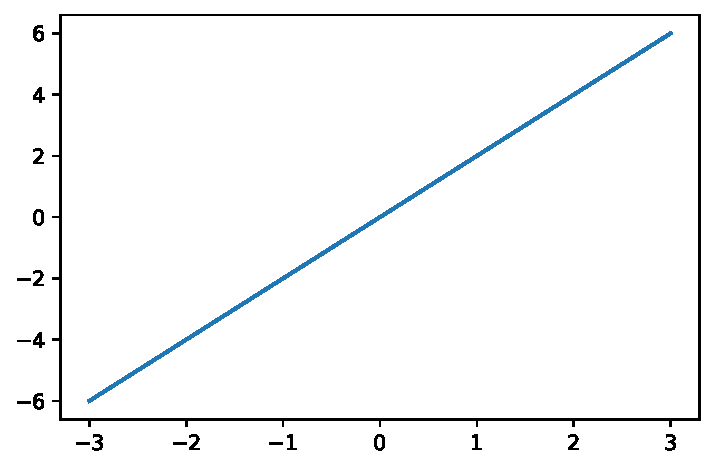
\includegraphics[keepaspectratio]{books/en-US/lab_files/figure-latex/cell-232-output-1.pdf}}

\begin{enumerate}
\def\labelenumi{\arabic{enumi}.}
\setcounter{enumi}{1}
\tightlist
\item
  Line not through the origin (affine subspace)
\end{enumerate}

\[
L' = \{ [3,1] + t \cdot [1,2] : t \in \mathbb{R} \}
\]

\begin{Shaded}
\begin{Highlighting}[]
\NormalTok{point }\OperatorTok{=}\NormalTok{ np.array([}\DecValTok{3}\NormalTok{,}\DecValTok{1}\NormalTok{])}
\NormalTok{direction }\OperatorTok{=}\NormalTok{ np.array([}\DecValTok{1}\NormalTok{,}\DecValTok{2}\NormalTok{])}
\NormalTok{line\_shifted }\OperatorTok{=}\NormalTok{ np.array([point }\OperatorTok{+}\NormalTok{ k}\OperatorTok{*}\NormalTok{direction }\ControlFlowTok{for}\NormalTok{ k }\KeywordTok{in}\NormalTok{ t])}
\NormalTok{plt.plot(line\_shifted[:,}\DecValTok{0}\NormalTok{], line\_shifted[:,}\DecValTok{1}\NormalTok{], label}\OperatorTok{=}\StringTok{"Shifted line"}\NormalTok{)}
\end{Highlighting}
\end{Shaded}

\pandocbounded{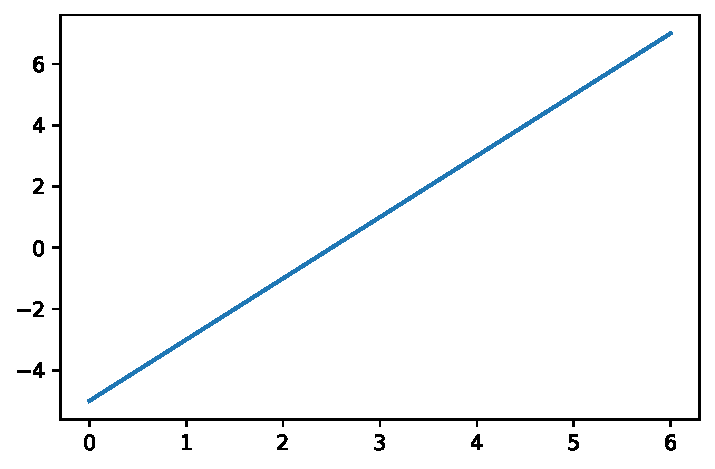
\includegraphics[keepaspectratio]{books/en-US/lab_files/figure-latex/cell-233-output-1.pdf}}

\begin{enumerate}
\def\labelenumi{\arabic{enumi}.}
\setcounter{enumi}{2}
\tightlist
\item
  Visualizing together
\end{enumerate}

\begin{Shaded}
\begin{Highlighting}[]
\NormalTok{plt.scatter(}\OperatorTok{*}\NormalTok{point, color}\OperatorTok{=}\StringTok{"red"}\NormalTok{, label}\OperatorTok{=}\StringTok{"Shift point"}\NormalTok{)}
\NormalTok{plt.axhline(}\DecValTok{0}\NormalTok{,color}\OperatorTok{=}\StringTok{\textquotesingle{}black\textquotesingle{}}\NormalTok{,linewidth}\OperatorTok{=}\FloatTok{0.5}\NormalTok{)}
\NormalTok{plt.axvline(}\DecValTok{0}\NormalTok{,color}\OperatorTok{=}\StringTok{\textquotesingle{}black\textquotesingle{}}\NormalTok{,linewidth}\OperatorTok{=}\FloatTok{0.5}\NormalTok{)}
\NormalTok{plt.legend()}
\NormalTok{plt.grid()}
\NormalTok{plt.show()}
\end{Highlighting}
\end{Shaded}

\pandocbounded{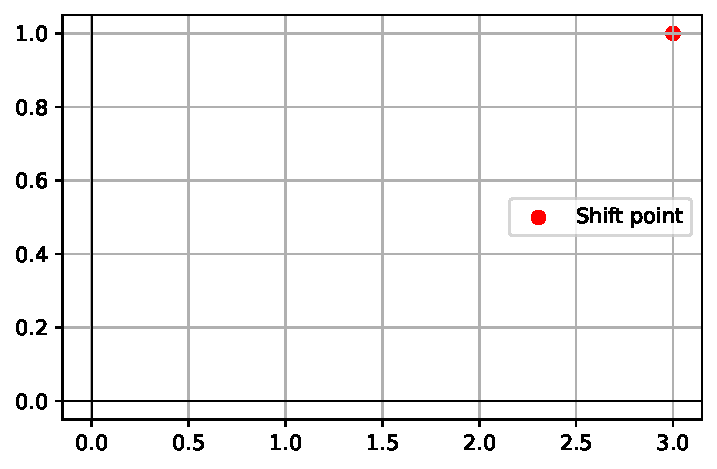
\includegraphics[keepaspectratio]{books/en-US/lab_files/figure-latex/cell-234-output-1.pdf}}

One line passes through the origin, the other is parallel but shifted.

\begin{enumerate}
\def\labelenumi{\arabic{enumi}.}
\setcounter{enumi}{3}
\tightlist
\item
  Plane example
\end{enumerate}

A plane in \(\mathbb{R}^3\):

\[
P = \{ [1,2,3] + s[1,0,0] + t[0,1,0] : s,t \in \mathbb{R} \}
\]

This is an affine plane parallel to the \(xy\)-plane, but shifted.

\begin{Shaded}
\begin{Highlighting}[]
\NormalTok{s\_vals }\OperatorTok{=}\NormalTok{ np.linspace(}\OperatorTok{{-}}\DecValTok{2}\NormalTok{,}\DecValTok{2}\NormalTok{,}\DecValTok{10}\NormalTok{)}
\NormalTok{t\_vals }\OperatorTok{=}\NormalTok{ np.linspace(}\OperatorTok{{-}}\DecValTok{2}\NormalTok{,}\DecValTok{2}\NormalTok{,}\DecValTok{10}\NormalTok{)}

\NormalTok{points }\OperatorTok{=}\NormalTok{ []}
\ControlFlowTok{for}\NormalTok{ s }\KeywordTok{in}\NormalTok{ s\_vals:}
    \ControlFlowTok{for}\NormalTok{ t }\KeywordTok{in}\NormalTok{ t\_vals:}
\NormalTok{        points.append([}\DecValTok{1}\NormalTok{,}\DecValTok{2}\NormalTok{,}\DecValTok{3}\NormalTok{] }\OperatorTok{+}\NormalTok{ s}\OperatorTok{*}\NormalTok{np.array([}\DecValTok{1}\NormalTok{,}\DecValTok{0}\NormalTok{,}\DecValTok{0}\NormalTok{]) }\OperatorTok{+}\NormalTok{ t}\OperatorTok{*}\NormalTok{np.array([}\DecValTok{0}\NormalTok{,}\DecValTok{1}\NormalTok{,}\DecValTok{0}\NormalTok{]))}

\NormalTok{points }\OperatorTok{=}\NormalTok{ np.array(points)}

\ImportTok{from}\NormalTok{ mpl\_toolkits.mplot3d }\ImportTok{import}\NormalTok{ Axes3D}
\NormalTok{fig }\OperatorTok{=}\NormalTok{ plt.figure()}
\NormalTok{ax }\OperatorTok{=}\NormalTok{ fig.add\_subplot(}\DecValTok{111}\NormalTok{, projection}\OperatorTok{=}\StringTok{\textquotesingle{}3d\textquotesingle{}}\NormalTok{)}
\NormalTok{ax.scatter(points[:,}\DecValTok{0}\NormalTok{], points[:,}\DecValTok{1}\NormalTok{], points[:,}\DecValTok{2}\NormalTok{])}
\NormalTok{ax.set\_title(}\StringTok{"Affine plane in R\^{}3"}\NormalTok{)}
\NormalTok{plt.show()}
\end{Highlighting}
\end{Shaded}

\pandocbounded{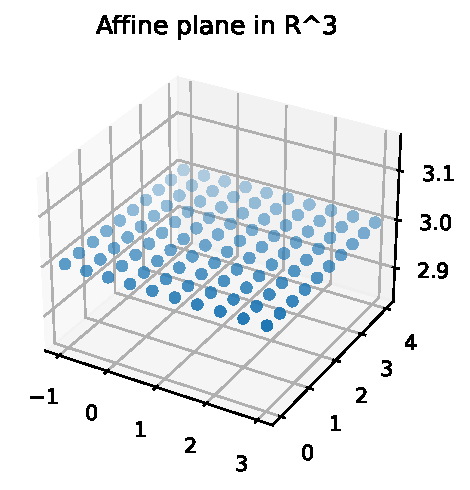
\includegraphics[keepaspectratio]{books/en-US/lab_files/figure-latex/cell-235-output-1.pdf}}

\begin{enumerate}
\def\labelenumi{\arabic{enumi}.}
\setcounter{enumi}{4}
\tightlist
\item
  Algebraic difference
\end{enumerate}

\begin{itemize}
\tightlist
\item
  A subspace must satisfy closure under addition and scalar
  multiplication, and must include 0.
\item
  An affine subspace is just a subspace plus a fixed shift vector.
\end{itemize}

\subsubsection{Try It Yourself}\label{try-it-yourself-138}

\begin{enumerate}
\def\labelenumi{\arabic{enumi}.}
\item
  Define a line in \(\mathbb{R}^2\):

  \[
  (x,y) = (2,3) + t(1,-1)
  \]

  Plot it and compare with the subspace spanned by \((1,-1)\).
\item
  Construct an affine plane in \(\mathbb{R}^3\) shifted by vector
  \((5,5,5)\).
\item
  Show algebraically that subtracting the shift point turns an affine
  subspace back into a regular subspace.
\end{enumerate}

\subsubsection{The Takeaway}\label{the-takeaway-22}

\begin{itemize}
\tightlist
\item
  Subspaces go through the origin.
\item
  Affine subspaces are shifted copies of subspaces.
\item
  They're essential in geometry, computer graphics, and optimization
  (e.g., feasible regions in linear programming).
\end{itemize}

\section{Chapter 5. Linear Transformation and
Structure}\label{chapter-5.-linear-transformation-and-structure-1}

\subsection{41. Linear Transformations (Preserving Lines and
Sums)}\label{linear-transformations-preserving-lines-and-sums}

A linear transformation is a function between vector spaces that
preserves two key properties:

\begin{enumerate}
\def\labelenumi{\arabic{enumi}.}
\tightlist
\item
  Additivity: \(T(u+v) = T(u) + T(v)\)
\item
  Homogeneity: \(T(cu) = cT(u)\)
\end{enumerate}

In practice, every linear transformation can be represented by a matrix.
This lab will help you understand and experiment with linear
transformations in Python.

\subsubsection{Set Up Your Lab}\label{set-up-your-lab-40}

\begin{Shaded}
\begin{Highlighting}[]
\ImportTok{import}\NormalTok{ numpy }\ImportTok{as}\NormalTok{ np}
\ImportTok{import}\NormalTok{ matplotlib.pyplot }\ImportTok{as}\NormalTok{ plt}
\end{Highlighting}
\end{Shaded}

\subsubsection{Step-by-Step Code
Walkthrough}\label{step-by-step-code-walkthrough-40}

\begin{enumerate}
\def\labelenumi{\arabic{enumi}.}
\tightlist
\item
  Simple linear transformation (scaling)
\end{enumerate}

Let's scale vectors by 2 in the x-direction and by 0.5 in the
y-direction.

\begin{Shaded}
\begin{Highlighting}[]
\NormalTok{A }\OperatorTok{=}\NormalTok{ np.array([}
\NormalTok{    [}\DecValTok{2}\NormalTok{, }\DecValTok{0}\NormalTok{],}
\NormalTok{    [}\DecValTok{0}\NormalTok{, }\FloatTok{0.5}\NormalTok{]}
\NormalTok{])}

\NormalTok{v }\OperatorTok{=}\NormalTok{ np.array([}\DecValTok{1}\NormalTok{, }\DecValTok{2}\NormalTok{])}
\NormalTok{Tv }\OperatorTok{=}\NormalTok{ A }\OperatorTok{@}\NormalTok{ v}
\BuiltInTok{print}\NormalTok{(}\StringTok{"Original v:"}\NormalTok{, v)}
\BuiltInTok{print}\NormalTok{(}\StringTok{"Transformed Tv:"}\NormalTok{, Tv)}
\end{Highlighting}
\end{Shaded}

\begin{verbatim}
Original v: [1 2]
Transformed Tv: [2. 1.]
\end{verbatim}

\begin{enumerate}
\def\labelenumi{\arabic{enumi}.}
\setcounter{enumi}{1}
\tightlist
\item
  Visualizing multiple vectors
\end{enumerate}

\begin{Shaded}
\begin{Highlighting}[]
\NormalTok{vectors }\OperatorTok{=}\NormalTok{ [np.array([}\DecValTok{1}\NormalTok{,}\DecValTok{1}\NormalTok{]), np.array([}\DecValTok{2}\NormalTok{,}\DecValTok{0}\NormalTok{]), np.array([}\OperatorTok{{-}}\DecValTok{1}\NormalTok{,}\DecValTok{2}\NormalTok{])]}

\ControlFlowTok{for}\NormalTok{ v }\KeywordTok{in}\NormalTok{ vectors:}
\NormalTok{    Tv }\OperatorTok{=}\NormalTok{ A }\OperatorTok{@}\NormalTok{ v}
\NormalTok{    plt.arrow(}\DecValTok{0}\NormalTok{,}\DecValTok{0}\NormalTok{,v[}\DecValTok{0}\NormalTok{],v[}\DecValTok{1}\NormalTok{],head\_width}\OperatorTok{=}\FloatTok{0.1}\NormalTok{,color}\OperatorTok{=}\StringTok{\textquotesingle{}blue\textquotesingle{}}\NormalTok{,length\_includes\_head}\OperatorTok{=}\VariableTok{True}\NormalTok{)}
\NormalTok{    plt.arrow(}\DecValTok{0}\NormalTok{,}\DecValTok{0}\NormalTok{,Tv[}\DecValTok{0}\NormalTok{],Tv[}\DecValTok{1}\NormalTok{],head\_width}\OperatorTok{=}\FloatTok{0.1}\NormalTok{,color}\OperatorTok{=}\StringTok{\textquotesingle{}red\textquotesingle{}}\NormalTok{,length\_includes\_head}\OperatorTok{=}\VariableTok{True}\NormalTok{)}

\NormalTok{plt.axhline(}\DecValTok{0}\NormalTok{,color}\OperatorTok{=}\StringTok{\textquotesingle{}black\textquotesingle{}}\NormalTok{,linewidth}\OperatorTok{=}\FloatTok{0.5}\NormalTok{)}
\NormalTok{plt.axvline(}\DecValTok{0}\NormalTok{,color}\OperatorTok{=}\StringTok{\textquotesingle{}black\textquotesingle{}}\NormalTok{,linewidth}\OperatorTok{=}\FloatTok{0.5}\NormalTok{)}
\NormalTok{plt.xlim(}\OperatorTok{{-}}\DecValTok{3}\NormalTok{,}\DecValTok{5}\NormalTok{)}
\NormalTok{plt.ylim(}\OperatorTok{{-}}\DecValTok{1}\NormalTok{,}\DecValTok{5}\NormalTok{)}
\NormalTok{plt.grid()}
\NormalTok{plt.title(}\StringTok{"Blue = original, Red = transformed"}\NormalTok{)}
\NormalTok{plt.show()}
\end{Highlighting}
\end{Shaded}

\pandocbounded{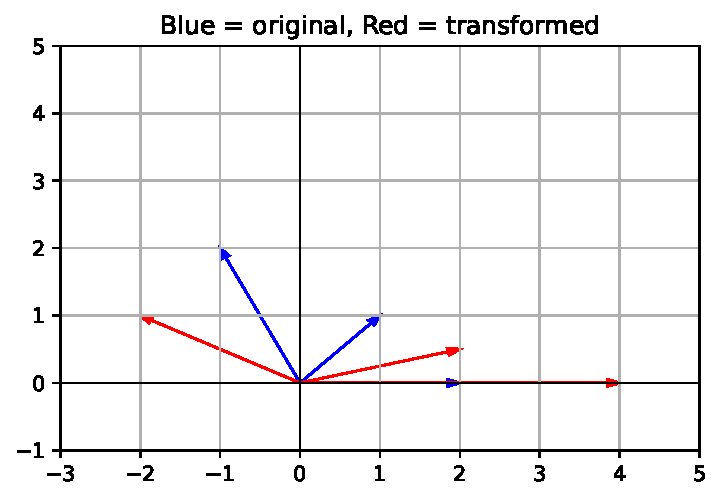
\includegraphics[keepaspectratio]{books/en-US/lab_files/figure-latex/cell-238-output-1.pdf}}

Blue arrows are the original vectors; red arrows are the transformed
ones. Notice how the transformation stretches and compresses
consistently.

\begin{enumerate}
\def\labelenumi{\arabic{enumi}.}
\setcounter{enumi}{2}
\tightlist
\item
  Rotation as a linear transformation
\end{enumerate}

Rotating vectors by \(\theta = 90^\circ\):

\begin{Shaded}
\begin{Highlighting}[]
\NormalTok{theta }\OperatorTok{=}\NormalTok{ np.pi}\OperatorTok{/}\DecValTok{2}
\NormalTok{R }\OperatorTok{=}\NormalTok{ np.array([}
\NormalTok{    [np.cos(theta), }\OperatorTok{{-}}\NormalTok{np.sin(theta)],}
\NormalTok{    [np.sin(theta),  np.cos(theta)]}
\NormalTok{])}

\NormalTok{v }\OperatorTok{=}\NormalTok{ np.array([}\DecValTok{1}\NormalTok{,}\DecValTok{0}\NormalTok{])}
\BuiltInTok{print}\NormalTok{(}\StringTok{"Rotate [1,0] by 90°:"}\NormalTok{, R }\OperatorTok{@}\NormalTok{ v)}
\end{Highlighting}
\end{Shaded}

\begin{verbatim}
Rotate [1,0] by 90°: [6.123234e-17 1.000000e+00]
\end{verbatim}

The result is \([0,1]\), a perfect rotation.

\begin{enumerate}
\def\labelenumi{\arabic{enumi}.}
\setcounter{enumi}{3}
\tightlist
\item
  Checking linearity
\end{enumerate}

\begin{Shaded}
\begin{Highlighting}[]
\NormalTok{u }\OperatorTok{=}\NormalTok{ np.array([}\DecValTok{1}\NormalTok{,}\DecValTok{2}\NormalTok{])}
\NormalTok{v }\OperatorTok{=}\NormalTok{ np.array([}\DecValTok{3}\NormalTok{,}\DecValTok{4}\NormalTok{])}
\NormalTok{c }\OperatorTok{=} \DecValTok{5}

\NormalTok{lhs }\OperatorTok{=}\NormalTok{ A }\OperatorTok{@}\NormalTok{ (u}\OperatorTok{+}\NormalTok{v)}
\NormalTok{rhs }\OperatorTok{=}\NormalTok{ A}\OperatorTok{@}\NormalTok{u }\OperatorTok{+}\NormalTok{ A}\OperatorTok{@}\NormalTok{v}
\BuiltInTok{print}\NormalTok{(}\StringTok{"Additivity holds?"}\NormalTok{, np.allclose(lhs,rhs))}

\NormalTok{lhs }\OperatorTok{=}\NormalTok{ A }\OperatorTok{@}\NormalTok{ (c}\OperatorTok{*}\NormalTok{u)}
\NormalTok{rhs }\OperatorTok{=}\NormalTok{ c}\OperatorTok{*}\NormalTok{(A}\OperatorTok{@}\NormalTok{u)}
\BuiltInTok{print}\NormalTok{(}\StringTok{"Homogeneity holds?"}\NormalTok{, np.allclose(lhs,rhs))}
\end{Highlighting}
\end{Shaded}

\begin{verbatim}
Additivity holds? True
Homogeneity holds? True
\end{verbatim}

Both checks return \texttt{True}, proving \(T\) is linear.

\begin{enumerate}
\def\labelenumi{\arabic{enumi}.}
\setcounter{enumi}{4}
\tightlist
\item
  Non-linear example (for contrast)
\end{enumerate}

A transformation like \(T(x,y) = (x^2, y)\) is not linear.

\begin{Shaded}
\begin{Highlighting}[]
\KeywordTok{def}\NormalTok{ nonlinear(v):}
    \ControlFlowTok{return}\NormalTok{ np.array([v[}\DecValTok{0}\NormalTok{]}\OperatorTok{**}\DecValTok{2}\NormalTok{, v[}\DecValTok{1}\NormalTok{]])}

\BuiltInTok{print}\NormalTok{(}\StringTok{"T([2,3]) ="}\NormalTok{, nonlinear(np.array([}\DecValTok{2}\NormalTok{,}\DecValTok{3}\NormalTok{])))}
\BuiltInTok{print}\NormalTok{(}\StringTok{"Check additivity:"}\NormalTok{, nonlinear(np.array([}\DecValTok{1}\NormalTok{,}\DecValTok{2}\NormalTok{])}\OperatorTok{+}\NormalTok{np.array([}\DecValTok{3}\NormalTok{,}\DecValTok{4}\NormalTok{])) }\OperatorTok{==}\NormalTok{ (nonlinear([}\DecValTok{1}\NormalTok{,}\DecValTok{2}\NormalTok{])}\OperatorTok{+}\NormalTok{nonlinear([}\DecValTok{3}\NormalTok{,}\DecValTok{4}\NormalTok{])))}
\end{Highlighting}
\end{Shaded}

\begin{verbatim}
T([2,3]) = [4 3]
Check additivity: [False  True]
\end{verbatim}

This fails the additivity test, so it's not linear.

\subsubsection{Try It Yourself}\label{try-it-yourself-139}

\begin{enumerate}
\def\labelenumi{\arabic{enumi}.}
\item
  Define a shear matrix

  \[
  S = \begin{bmatrix} 1 & 1 \\ 0 & 1 \end{bmatrix}
  \]

  Apply it to vectors and plot before/after.
\item
  Verify linearity for rotation by 45°.
\item
  Test whether \(T(x,y) = (x+y, y)\) is linear.
\end{enumerate}

\subsubsection{The Takeaway}\label{the-takeaway-23}

\begin{itemize}
\tightlist
\item
  A linear transformation preserves vector addition and scalar
  multiplication.
\item
  Every linear transformation can be represented by a matrix.
\item
  Visualizing with arrows helps build geometric intuition: stretching,
  rotating, and shearing are all linear.
\end{itemize}

\subsection{42. Matrix Representation of a Linear Map (Choosing a
Basis)}\label{matrix-representation-of-a-linear-map-choosing-a-basis}

Every linear transformation can be written as a matrix, but the exact
matrix depends on the basis you choose. This lab shows how to build and
interpret matrix representations.

\subsubsection{Set Up Your Lab}\label{set-up-your-lab-41}

\begin{Shaded}
\begin{Highlighting}[]
\ImportTok{import}\NormalTok{ numpy }\ImportTok{as}\NormalTok{ np}
\ImportTok{from}\NormalTok{ sympy }\ImportTok{import}\NormalTok{ Matrix}
\end{Highlighting}
\end{Shaded}

\subsubsection{Step-by-Step Code
Walkthrough}\label{step-by-step-code-walkthrough-41}

\begin{enumerate}
\def\labelenumi{\arabic{enumi}.}
\tightlist
\item
  From transformation to matrix
\end{enumerate}

Suppose \(T: \mathbb{R}^2 \to \mathbb{R}^2\) is defined by:

\[
T(x,y) = (2x + y, \; x - y)
\]

To find its matrix in the standard basis, apply \(T\) to each basis
vector:

\begin{Shaded}
\begin{Highlighting}[]
\NormalTok{e1 }\OperatorTok{=}\NormalTok{ Matrix([}\DecValTok{1}\NormalTok{,}\DecValTok{0}\NormalTok{])}
\NormalTok{e2 }\OperatorTok{=}\NormalTok{ Matrix([}\DecValTok{0}\NormalTok{,}\DecValTok{1}\NormalTok{])}

\KeywordTok{def}\NormalTok{ T(v):}
\NormalTok{    x, y }\OperatorTok{=}\NormalTok{ v}
    \ControlFlowTok{return}\NormalTok{ Matrix([}\DecValTok{2}\OperatorTok{*}\NormalTok{x }\OperatorTok{+}\NormalTok{ y, x }\OperatorTok{{-}}\NormalTok{ y])}

\BuiltInTok{print}\NormalTok{(}\StringTok{"T(e1):"}\NormalTok{, T(e1))}
\BuiltInTok{print}\NormalTok{(}\StringTok{"T(e2):"}\NormalTok{, T(e2))}
\end{Highlighting}
\end{Shaded}

\begin{verbatim}
T(e1): Matrix([[2], [1]])
T(e2): Matrix([[1], [-1]])
\end{verbatim}

Stacking results as columns gives the matrix:

\begin{Shaded}
\begin{Highlighting}[]
\NormalTok{A }\OperatorTok{=}\NormalTok{ Matrix.hstack(T(e1), T(e2))}
\BuiltInTok{print}\NormalTok{(}\StringTok{"Matrix representation in standard basis:}\CharTok{\textbackslash{}n}\StringTok{"}\NormalTok{, A)}
\end{Highlighting}
\end{Shaded}

\begin{verbatim}
Matrix representation in standard basis:
 Matrix([[2, 1], [1, -1]])
\end{verbatim}

\begin{enumerate}
\def\labelenumi{\arabic{enumi}.}
\setcounter{enumi}{1}
\tightlist
\item
  Using the matrix for computations
\end{enumerate}

\begin{Shaded}
\begin{Highlighting}[]
\NormalTok{v }\OperatorTok{=}\NormalTok{ Matrix([}\DecValTok{3}\NormalTok{,}\DecValTok{4}\NormalTok{])}
\BuiltInTok{print}\NormalTok{(}\StringTok{"T(v) via definition:"}\NormalTok{, T(v))}
\BuiltInTok{print}\NormalTok{(}\StringTok{"T(v) via matrix:"}\NormalTok{, A}\OperatorTok{*}\NormalTok{v)}
\end{Highlighting}
\end{Shaded}

\begin{verbatim}
T(v) via definition: Matrix([[10], [-1]])
T(v) via matrix: Matrix([[10], [-1]])
\end{verbatim}

Both methods match.

\begin{enumerate}
\def\labelenumi{\arabic{enumi}.}
\setcounter{enumi}{2}
\tightlist
\item
  Matrix in a different basis
\end{enumerate}

Now suppose we use basis

\[
B = \{ [1,1], [1,-1] \}
\]

To represent \(T\) in this basis:

\begin{enumerate}
\def\labelenumi{\arabic{enumi}.}
\tightlist
\item
  Build the change-of-basis matrix \(P\).
\item
  Compute \(A_B = P^{-1}AP\).
\end{enumerate}

\begin{Shaded}
\begin{Highlighting}[]
\NormalTok{B }\OperatorTok{=}\NormalTok{ Matrix.hstack(Matrix([}\DecValTok{1}\NormalTok{,}\DecValTok{1}\NormalTok{]), Matrix([}\DecValTok{1}\NormalTok{,}\OperatorTok{{-}}\DecValTok{1}\NormalTok{]))}
\NormalTok{P }\OperatorTok{=}\NormalTok{ B}
\NormalTok{A\_B }\OperatorTok{=}\NormalTok{ P.inv() }\OperatorTok{*}\NormalTok{ A }\OperatorTok{*}\NormalTok{ P}
\BuiltInTok{print}\NormalTok{(}\StringTok{"Matrix representation in new basis:}\CharTok{\textbackslash{}n}\StringTok{"}\NormalTok{, A\_B)}
\end{Highlighting}
\end{Shaded}

\begin{verbatim}
Matrix representation in new basis:
 Matrix([[3/2, 3/2], [3/2, -1/2]])
\end{verbatim}

\begin{enumerate}
\def\labelenumi{\arabic{enumi}.}
\setcounter{enumi}{3}
\tightlist
\item
  Interpretation
\end{enumerate}

\begin{itemize}
\tightlist
\item
  In standard basis, \(A\) tells us how \(T\) acts on unit vectors.
\item
  In basis \(B\), \(A_B\) shows how \(T\) looks when described using
  different coordinates.
\end{itemize}

\begin{enumerate}
\def\labelenumi{\arabic{enumi}.}
\setcounter{enumi}{4}
\tightlist
\item
  Random linear map in \(\mathbb{R}^3\)
\end{enumerate}

\begin{Shaded}
\begin{Highlighting}[]
\NormalTok{np.random.seed(}\DecValTok{1}\NormalTok{)}
\NormalTok{A3 }\OperatorTok{=}\NormalTok{ Matrix(np.random.randint(}\OperatorTok{{-}}\DecValTok{3}\NormalTok{,}\DecValTok{4}\NormalTok{,(}\DecValTok{3}\NormalTok{,}\DecValTok{3}\NormalTok{)))}
\BuiltInTok{print}\NormalTok{(}\StringTok{"Random transformation matrix:}\CharTok{\textbackslash{}n}\StringTok{"}\NormalTok{, A3)}

\NormalTok{B3 }\OperatorTok{=}\NormalTok{ Matrix.hstack(Matrix([}\DecValTok{1}\NormalTok{,}\DecValTok{0}\NormalTok{,}\DecValTok{1}\NormalTok{]), Matrix([}\DecValTok{0}\NormalTok{,}\DecValTok{1}\NormalTok{,}\DecValTok{1}\NormalTok{]), Matrix([}\DecValTok{1}\NormalTok{,}\DecValTok{1}\NormalTok{,}\DecValTok{0}\NormalTok{]))}
\NormalTok{A3\_B }\OperatorTok{=}\NormalTok{ B3.inv() }\OperatorTok{*}\NormalTok{ A3 }\OperatorTok{*}\NormalTok{ B3}
\BuiltInTok{print}\NormalTok{(}\StringTok{"Representation in new basis:}\CharTok{\textbackslash{}n}\StringTok{"}\NormalTok{, A3\_B)}
\end{Highlighting}
\end{Shaded}

\begin{verbatim}
Random transformation matrix:
 Matrix([[2, 0, 1], [-3, -2, 0], [2, -3, -3]])
Representation in new basis:
 Matrix([[5/2, -3/2, 3], [-7/2, -9/2, -4], [1/2, 5/2, -1]])
\end{verbatim}

\subsubsection{Try It Yourself}\label{try-it-yourself-140}

\begin{enumerate}
\def\labelenumi{\arabic{enumi}.}
\tightlist
\item
  Define \(T(x,y) = (x+2y, 3x+y)\). Find its matrix in the standard
  basis.
\item
  Use a new basis \(\{[2,0],[0,3]\}\). Compute the representation
  \(A_B\).
\item
  Verify that applying \(T\) directly to a vector matches computing via
  \(A_B\) and change-of-basis.
\end{enumerate}

\subsubsection{The Takeaway}\label{the-takeaway-24}

\begin{itemize}
\tightlist
\item
  A linear transformation becomes a matrix representation once a basis
  is chosen.
\item
  Columns of the matrix = images of basis vectors.
\item
  Changing the basis changes the matrix, but the transformation itself
  stays the same.
\end{itemize}

\subsection{43. Kernel and Image (Inputs That Vanish; Outputs We Can
Reach)}\label{kernel-and-image-inputs-that-vanish-outputs-we-can-reach}

Two fundamental subspaces describe any linear transformation
\(T(x) = Ax\):

\begin{itemize}
\tightlist
\item
  Kernel (null space): all vectors \(x\) such that \(Ax = 0\).
\item
  Image (column space): all possible outputs \(Ax\).
\end{itemize}

The kernel tells us what inputs collapse to zero, while the image tells
us what outputs are achievable.

\subsubsection{Set Up Your Lab}\label{set-up-your-lab-42}

\begin{Shaded}
\begin{Highlighting}[]
\ImportTok{import}\NormalTok{ numpy }\ImportTok{as}\NormalTok{ np}
\ImportTok{from}\NormalTok{ sympy }\ImportTok{import}\NormalTok{ Matrix}
\end{Highlighting}
\end{Shaded}

\subsubsection{Step-by-Step Code
Walkthrough}\label{step-by-step-code-walkthrough-42}

\begin{enumerate}
\def\labelenumi{\arabic{enumi}.}
\tightlist
\item
  Kernel of a matrix
\end{enumerate}

Consider

\[
A = \begin{bmatrix} 1 & 2 & 3 \\ 2 & 4 & 6 \end{bmatrix}
\]

\begin{Shaded}
\begin{Highlighting}[]
\NormalTok{A }\OperatorTok{=}\NormalTok{ Matrix([}
\NormalTok{    [}\DecValTok{1}\NormalTok{,}\DecValTok{2}\NormalTok{,}\DecValTok{3}\NormalTok{],}
\NormalTok{    [}\DecValTok{2}\NormalTok{,}\DecValTok{4}\NormalTok{,}\DecValTok{6}\NormalTok{]}
\NormalTok{])}

\BuiltInTok{print}\NormalTok{(}\StringTok{"Null space (kernel):"}\NormalTok{, A.nullspace())}
\end{Highlighting}
\end{Shaded}

\begin{verbatim}
Null space (kernel): [Matrix([
[-2],
[ 1],
[ 0]]), Matrix([
[-3],
[ 0],
[ 1]])]
\end{verbatim}

The null space basis shows dependencies among columns. Here, the kernel
is 2-dimensional because columns are dependent.

\begin{enumerate}
\def\labelenumi{\arabic{enumi}.}
\setcounter{enumi}{1}
\tightlist
\item
  Image (column space)
\end{enumerate}

\begin{Shaded}
\begin{Highlighting}[]
\BuiltInTok{print}\NormalTok{(}\StringTok{"Column space (image):"}\NormalTok{, A.columnspace())}
\BuiltInTok{print}\NormalTok{(}\StringTok{"Rank (dimension of image):"}\NormalTok{, A.rank())}
\end{Highlighting}
\end{Shaded}

\begin{verbatim}
Column space (image): [Matrix([
[1],
[2]])]
Rank (dimension of image): 1
\end{verbatim}

The image is spanned by \([1,2]^T\). So all outputs of \(A\) are
multiples of this vector.

\begin{enumerate}
\def\labelenumi{\arabic{enumi}.}
\setcounter{enumi}{2}
\tightlist
\item
  Interpretation
\end{enumerate}

\begin{itemize}
\tightlist
\item
  Kernel vectors → directions that map to zero.
\item
  Image vectors → directions we can actually reach in the output space.
\end{itemize}

If \(x \in \ker(A)\), then \(Ax = 0\). If \(b\) is not in the image, the
system \(Ax = b\) has no solution.

\begin{enumerate}
\def\labelenumi{\arabic{enumi}.}
\setcounter{enumi}{3}
\tightlist
\item
  Example with full rank
\end{enumerate}

\begin{Shaded}
\begin{Highlighting}[]
\NormalTok{B }\OperatorTok{=}\NormalTok{ Matrix([}
\NormalTok{    [}\DecValTok{1}\NormalTok{,}\DecValTok{0}\NormalTok{,}\DecValTok{0}\NormalTok{],}
\NormalTok{    [}\DecValTok{0}\NormalTok{,}\DecValTok{1}\NormalTok{,}\DecValTok{0}\NormalTok{],}
\NormalTok{    [}\DecValTok{0}\NormalTok{,}\DecValTok{0}\NormalTok{,}\DecValTok{1}\NormalTok{]}
\NormalTok{])}

\BuiltInTok{print}\NormalTok{(}\StringTok{"Kernel of B:"}\NormalTok{, B.nullspace())}
\BuiltInTok{print}\NormalTok{(}\StringTok{"Image of B:"}\NormalTok{, B.columnspace())}
\end{Highlighting}
\end{Shaded}

\begin{verbatim}
Kernel of B: []
Image of B: [Matrix([
[1],
[0],
[0]]), Matrix([
[0],
[1],
[0]]), Matrix([
[0],
[0],
[1]])]
\end{verbatim}

\begin{itemize}
\tightlist
\item
  Kernel = only zero vector.
\item
  Image = all of \(\mathbb{R}^3\).
\end{itemize}

\begin{enumerate}
\def\labelenumi{\arabic{enumi}.}
\setcounter{enumi}{4}
\tightlist
\item
  NumPy version (image via column space)
\end{enumerate}

\begin{Shaded}
\begin{Highlighting}[]
\NormalTok{A }\OperatorTok{=}\NormalTok{ np.array([[}\DecValTok{1}\NormalTok{,}\DecValTok{2}\NormalTok{,}\DecValTok{3}\NormalTok{],[}\DecValTok{2}\NormalTok{,}\DecValTok{4}\NormalTok{,}\DecValTok{6}\NormalTok{]], dtype}\OperatorTok{=}\BuiltInTok{float}\NormalTok{)}
\NormalTok{rank }\OperatorTok{=}\NormalTok{ np.linalg.matrix\_rank(A)}
\BuiltInTok{print}\NormalTok{(}\StringTok{"Rank with NumPy:"}\NormalTok{, rank)}
\end{Highlighting}
\end{Shaded}

\begin{verbatim}
Rank with NumPy: 1
\end{verbatim}

NumPy doesn't compute null spaces directly, but we can use SVD for that
if needed.

\subsubsection{Try It Yourself}\label{try-it-yourself-141}

\begin{enumerate}
\def\labelenumi{\arabic{enumi}.}
\item
  Compute kernel and image for

  \[
  \begin{bmatrix} 1 & 1 \\ 1 & 1 \end{bmatrix}
  \]

  What do they look like?
\item
  Take a random 3×4 matrix and find its kernel and image dimensions.
\item
  Solve \(Ax = b\) for a matrix \(A\). Try two different \(b\): one
  inside the image, one outside. Observe the difference.
\end{enumerate}

\subsubsection{The Takeaway}\label{the-takeaway-25}

\begin{itemize}
\tightlist
\item
  Kernel = inputs that vanish under \(A\).
\item
  Image = outputs that can be reached by \(A\).
\item
  Together, they fully describe what a linear map does: what it
  ``kills'' and what it ``produces.''
\end{itemize}

\subsection{44. Invertibility and Isomorphisms (Perfectly Reversible
Maps)}\label{invertibility-and-isomorphisms-perfectly-reversible-maps}

A matrix (or linear map) is invertible if it has an inverse \(A^{-1}\)
such that

\[
A^{-1}A = I \quad \text{and} \quad AA^{-1} = I
\]

An invertible map is also called an isomorphism, because it preserves
all information - every input has exactly one output, and every output
comes from exactly one input.

\subsubsection{Set Up Your Lab}\label{set-up-your-lab-43}

\begin{Shaded}
\begin{Highlighting}[]
\ImportTok{import}\NormalTok{ numpy }\ImportTok{as}\NormalTok{ np}
\ImportTok{from}\NormalTok{ sympy }\ImportTok{import}\NormalTok{ Matrix}
\end{Highlighting}
\end{Shaded}

\subsubsection{Step-by-Step Code
Walkthrough}\label{step-by-step-code-walkthrough-43}

\begin{enumerate}
\def\labelenumi{\arabic{enumi}.}
\tightlist
\item
  Checking invertibility
\end{enumerate}

\begin{Shaded}
\begin{Highlighting}[]
\NormalTok{A }\OperatorTok{=}\NormalTok{ Matrix([}
\NormalTok{    [}\DecValTok{2}\NormalTok{,}\DecValTok{1}\NormalTok{],}
\NormalTok{    [}\DecValTok{5}\NormalTok{,}\DecValTok{3}\NormalTok{]}
\NormalTok{])}

\BuiltInTok{print}\NormalTok{(}\StringTok{"Determinant:"}\NormalTok{, A.det())}
\BuiltInTok{print}\NormalTok{(}\StringTok{"Is invertible?"}\NormalTok{, A.det() }\OperatorTok{!=} \DecValTok{0}\NormalTok{)}
\end{Highlighting}
\end{Shaded}

\begin{verbatim}
Determinant: 1
Is invertible? True
\end{verbatim}

If determinant ≠ 0 → invertible.

\begin{enumerate}
\def\labelenumi{\arabic{enumi}.}
\setcounter{enumi}{1}
\tightlist
\item
  Computing the inverse
\end{enumerate}

\begin{Shaded}
\begin{Highlighting}[]
\NormalTok{A\_inv }\OperatorTok{=}\NormalTok{ A.inv()}
\BuiltInTok{print}\NormalTok{(}\StringTok{"Inverse matrix:}\CharTok{\textbackslash{}n}\StringTok{"}\NormalTok{, A\_inv)}

\BuiltInTok{print}\NormalTok{(}\StringTok{"Check A*A\_inv = I:}\CharTok{\textbackslash{}n}\StringTok{"}\NormalTok{, A }\OperatorTok{*}\NormalTok{ A\_inv)}
\end{Highlighting}
\end{Shaded}

\begin{verbatim}
Inverse matrix:
 Matrix([[3, -1], [-5, 2]])
Check A*A_inv = I:
 Matrix([[1, 0], [0, 1]])
\end{verbatim}

\begin{enumerate}
\def\labelenumi{\arabic{enumi}.}
\setcounter{enumi}{2}
\tightlist
\item
  Solving systems with inverses
\end{enumerate}

For \(Ax = b\), if \(A\) is invertible:

\begin{Shaded}
\begin{Highlighting}[]
\NormalTok{b }\OperatorTok{=}\NormalTok{ Matrix([}\DecValTok{1}\NormalTok{,}\DecValTok{2}\NormalTok{])}
\NormalTok{x }\OperatorTok{=}\NormalTok{ A\_inv }\OperatorTok{*}\NormalTok{ b}
\BuiltInTok{print}\NormalTok{(}\StringTok{"Solution x:"}\NormalTok{, x)}
\end{Highlighting}
\end{Shaded}

\begin{verbatim}
Solution x: Matrix([[1], [-1]])
\end{verbatim}

This is equivalent to \texttt{A.solve(b)} in SymPy or
\texttt{np.linalg.solve} in NumPy.

\begin{enumerate}
\def\labelenumi{\arabic{enumi}.}
\setcounter{enumi}{3}
\tightlist
\item
  Non-invertible (singular) example
\end{enumerate}

\begin{Shaded}
\begin{Highlighting}[]
\NormalTok{B }\OperatorTok{=}\NormalTok{ Matrix([}
\NormalTok{    [}\DecValTok{1}\NormalTok{,}\DecValTok{2}\NormalTok{],}
\NormalTok{    [}\DecValTok{2}\NormalTok{,}\DecValTok{4}\NormalTok{]}
\NormalTok{])}

\BuiltInTok{print}\NormalTok{(}\StringTok{"Determinant:"}\NormalTok{, B.det())}
\BuiltInTok{print}\NormalTok{(}\StringTok{"Is invertible?"}\NormalTok{, B.det() }\OperatorTok{!=} \DecValTok{0}\NormalTok{)}
\end{Highlighting}
\end{Shaded}

\begin{verbatim}
Determinant: 0
Is invertible? False
\end{verbatim}

Determinant = 0 → no inverse. The matrix collapses space onto a line,
losing information.

\begin{enumerate}
\def\labelenumi{\arabic{enumi}.}
\setcounter{enumi}{4}
\tightlist
\item
  NumPy version
\end{enumerate}

\begin{Shaded}
\begin{Highlighting}[]
\NormalTok{A }\OperatorTok{=}\NormalTok{ np.array([[}\DecValTok{2}\NormalTok{,}\DecValTok{1}\NormalTok{],[}\DecValTok{5}\NormalTok{,}\DecValTok{3}\NormalTok{]], dtype}\OperatorTok{=}\BuiltInTok{float}\NormalTok{)}
\BuiltInTok{print}\NormalTok{(}\StringTok{"Determinant:"}\NormalTok{, np.linalg.det(A))}
\BuiltInTok{print}\NormalTok{(}\StringTok{"Inverse:}\CharTok{\textbackslash{}n}\StringTok{"}\NormalTok{, np.linalg.inv(A))}
\end{Highlighting}
\end{Shaded}

\begin{verbatim}
Determinant: 1.0000000000000002
Inverse:
 [[ 3. -1.]
 [-5.  2.]]
\end{verbatim}

\begin{enumerate}
\def\labelenumi{\arabic{enumi}.}
\setcounter{enumi}{5}
\tightlist
\item
  Geometric intuition
\end{enumerate}

\begin{itemize}
\tightlist
\item
  Invertible transformation = reversible (like rotating, scaling by
  nonzero).
\item
  Non-invertible transformation = squashing space into a lower dimension
  (like flattening a plane onto a line).
\end{itemize}

\subsubsection{Try It Yourself}\label{try-it-yourself-142}

\begin{enumerate}
\def\labelenumi{\arabic{enumi}.}
\item
  Test whether

  \[
  \begin{bmatrix} 1 & 0 \\ 0 & 1 \end{bmatrix}
  \]

  is invertible and find its inverse.
\item
  Compute the determinant of a 3×3 random integer matrix. If it's
  nonzero, find its inverse.
\item
  Create a singular 3×3 matrix (make one row a multiple of another).
  Confirm it has no inverse.
\end{enumerate}

\subsubsection{The Takeaway}\label{the-takeaway-26}

\begin{itemize}
\tightlist
\item
  Invertible matrix ↔ isomorphism: perfectly reversible, no information
  lost.
\item
  Determinant ≠ 0 → invertible; determinant = 0 → singular.
\item
  Inverses are useful conceptually, but in computation we usually solve
  systems directly instead of calculating \(A^{-1}\).
\end{itemize}

\subsection{45. Composition, Powers, and Iteration (Doing It Again and
Again)}\label{composition-powers-and-iteration-doing-it-again-and-again}

Linear transformations can be chained together. Applying one after
another is called composition, and in matrix form this becomes
multiplication. Repeated application of the same transformation leads to
powers of a matrix.

\subsubsection{Set Up Your Lab}\label{set-up-your-lab-44}

\begin{Shaded}
\begin{Highlighting}[]
\ImportTok{import}\NormalTok{ numpy }\ImportTok{as}\NormalTok{ np}
\ImportTok{from}\NormalTok{ sympy }\ImportTok{import}\NormalTok{ Matrix}
\end{Highlighting}
\end{Shaded}

\subsubsection{Step-by-Step Code
Walkthrough}\label{step-by-step-code-walkthrough-44}

\begin{enumerate}
\def\labelenumi{\arabic{enumi}.}
\tightlist
\item
  Composition of transformations
\end{enumerate}

Suppose we have two linear maps:

\begin{itemize}
\tightlist
\item
  \(T_1\): rotate by 90°
\item
  \(T_2\): scale x by 2
\end{itemize}

\begin{Shaded}
\begin{Highlighting}[]
\NormalTok{theta }\OperatorTok{=}\NormalTok{ np.pi}\OperatorTok{/}\DecValTok{2}
\NormalTok{R }\OperatorTok{=}\NormalTok{ np.array([}
\NormalTok{    [np.cos(theta), }\OperatorTok{{-}}\NormalTok{np.sin(theta)],}
\NormalTok{    [np.sin(theta),  np.cos(theta)]}
\NormalTok{])}
\NormalTok{S }\OperatorTok{=}\NormalTok{ np.array([}
\NormalTok{    [}\DecValTok{2}\NormalTok{,}\DecValTok{0}\NormalTok{],}
\NormalTok{    [}\DecValTok{0}\NormalTok{,}\DecValTok{1}\NormalTok{]}
\NormalTok{])}

\CommentTok{\# Compose: apply R then S}
\NormalTok{C }\OperatorTok{=}\NormalTok{ S }\OperatorTok{@}\NormalTok{ R}
\BuiltInTok{print}\NormalTok{(}\StringTok{"Composite matrix:}\CharTok{\textbackslash{}n}\StringTok{"}\NormalTok{, C)}
\end{Highlighting}
\end{Shaded}

\begin{verbatim}
Composite matrix:
 [[ 1.2246468e-16 -2.0000000e+00]
 [ 1.0000000e+00  6.1232340e-17]]
\end{verbatim}

Applying the composite matrix is equivalent to applying both maps in
sequence.

\begin{enumerate}
\def\labelenumi{\arabic{enumi}.}
\setcounter{enumi}{1}
\tightlist
\item
  Verifying with a vector
\end{enumerate}

\begin{Shaded}
\begin{Highlighting}[]
\NormalTok{v }\OperatorTok{=}\NormalTok{ np.array([}\DecValTok{1}\NormalTok{,}\DecValTok{1}\NormalTok{])}
\NormalTok{step1 }\OperatorTok{=}\NormalTok{ R }\OperatorTok{@}\NormalTok{ v}
\NormalTok{step2 }\OperatorTok{=}\NormalTok{ S }\OperatorTok{@}\NormalTok{ step1}
\NormalTok{composite }\OperatorTok{=}\NormalTok{ C }\OperatorTok{@}\NormalTok{ v}

\BuiltInTok{print}\NormalTok{(}\StringTok{"Step{-}by{-}step:"}\NormalTok{, step2)}
\BuiltInTok{print}\NormalTok{(}\StringTok{"Composite:"}\NormalTok{, composite)}
\end{Highlighting}
\end{Shaded}

\begin{verbatim}
Step-by-step: [-2.  1.]
Composite: [-2.  1.]
\end{verbatim}

Both results are the same → composition = matrix multiplication.

\begin{enumerate}
\def\labelenumi{\arabic{enumi}.}
\setcounter{enumi}{2}
\tightlist
\item
  Powers of a matrix
\end{enumerate}

Repeatedly applying a transformation corresponds to matrix powers.

Example: scaling by 2.

\begin{Shaded}
\begin{Highlighting}[]
\NormalTok{A }\OperatorTok{=}\NormalTok{ np.array([[}\DecValTok{2}\NormalTok{,}\DecValTok{0}\NormalTok{],[}\DecValTok{0}\NormalTok{,}\DecValTok{2}\NormalTok{]])}
\NormalTok{v }\OperatorTok{=}\NormalTok{ np.array([}\DecValTok{1}\NormalTok{,}\DecValTok{1}\NormalTok{])}

\BuiltInTok{print}\NormalTok{(}\StringTok{"A @ v ="}\NormalTok{, A }\OperatorTok{@}\NormalTok{ v)}
\BuiltInTok{print}\NormalTok{(}\StringTok{"A\^{}2 @ v ="}\NormalTok{, np.linalg.matrix\_power(A,}\DecValTok{2}\NormalTok{) }\OperatorTok{@}\NormalTok{ v)}
\BuiltInTok{print}\NormalTok{(}\StringTok{"A\^{}5 @ v ="}\NormalTok{, np.linalg.matrix\_power(A,}\DecValTok{5}\NormalTok{) }\OperatorTok{@}\NormalTok{ v)}
\end{Highlighting}
\end{Shaded}

\begin{verbatim}
A @ v = [2 2]
A^2 @ v = [4 4]
A^5 @ v = [32 32]
\end{verbatim}

Each step doubles the scaling effect.

\begin{enumerate}
\def\labelenumi{\arabic{enumi}.}
\setcounter{enumi}{3}
\tightlist
\item
  Iteration dynamics
\end{enumerate}

Let's iterate a transformation many times and see what happens.

Example:

\[
A = \begin{bmatrix} 0.5 & 0 \\ 0 & 0.5 \end{bmatrix}
\]

\begin{Shaded}
\begin{Highlighting}[]
\NormalTok{A }\OperatorTok{=}\NormalTok{ np.array([[}\FloatTok{0.5}\NormalTok{,}\DecValTok{0}\NormalTok{],[}\DecValTok{0}\NormalTok{,}\FloatTok{0.5}\NormalTok{]])}
\NormalTok{v }\OperatorTok{=}\NormalTok{ np.array([}\DecValTok{4}\NormalTok{,}\DecValTok{4}\NormalTok{])}

\ControlFlowTok{for}\NormalTok{ i }\KeywordTok{in} \BuiltInTok{range}\NormalTok{(}\DecValTok{5}\NormalTok{):}
\NormalTok{    v }\OperatorTok{=}\NormalTok{ A }\OperatorTok{@}\NormalTok{ v}
    \BuiltInTok{print}\NormalTok{(}\SpecialStringTok{f"Step }\SpecialCharTok{\{}\NormalTok{i}\OperatorTok{+}\DecValTok{1}\SpecialCharTok{\}}\SpecialStringTok{:"}\NormalTok{, v)}
\end{Highlighting}
\end{Shaded}

\begin{verbatim}
Step 1: [2. 2.]
Step 2: [1. 1.]
Step 3: [0.5 0.5]
Step 4: [0.25 0.25]
Step 5: [0.125 0.125]
\end{verbatim}

Each step shrinks the vector → iteration can reveal stability.

\begin{enumerate}
\def\labelenumi{\arabic{enumi}.}
\setcounter{enumi}{4}
\tightlist
\item
  Random example
\end{enumerate}

\begin{Shaded}
\begin{Highlighting}[]
\NormalTok{np.random.seed(}\DecValTok{0}\NormalTok{)}
\NormalTok{M }\OperatorTok{=}\NormalTok{ np.random.randint(}\OperatorTok{{-}}\DecValTok{2}\NormalTok{,}\DecValTok{3}\NormalTok{,(}\DecValTok{2}\NormalTok{,}\DecValTok{2}\NormalTok{))}
\BuiltInTok{print}\NormalTok{(}\StringTok{"Random matrix:}\CharTok{\textbackslash{}n}\StringTok{"}\NormalTok{, M)}

\BuiltInTok{print}\NormalTok{(}\StringTok{"M\^{}2:}\CharTok{\textbackslash{}n}\StringTok{"}\NormalTok{, np.linalg.matrix\_power(M,}\DecValTok{2}\NormalTok{))}
\BuiltInTok{print}\NormalTok{(}\StringTok{"M\^{}3:}\CharTok{\textbackslash{}n}\StringTok{"}\NormalTok{, np.linalg.matrix\_power(M,}\DecValTok{3}\NormalTok{))}
\end{Highlighting}
\end{Shaded}

\begin{verbatim}
Random matrix:
 [[ 2 -2]
 [ 1  1]]
M^2:
 [[ 2 -6]
 [ 3 -1]]
M^3:
 [[ -2 -10]
 [  5  -7]]
\end{verbatim}

\subsubsection{Try It Yourself}\label{try-it-yourself-143}

\begin{enumerate}
\def\labelenumi{\arabic{enumi}.}
\tightlist
\item
  Create two transformations: reflection across x-axis and scaling by 3.
  Compose them.
\item
  Take a shear matrix and compute \(A^5\). What happens to a vector
  after repeated application?
\item
  Experiment with a rotation matrix raised to higher powers. What cycle
  do you see?
\end{enumerate}

\subsubsection{The Takeaway}\label{the-takeaway-27}

\begin{itemize}
\tightlist
\item
  Composition of linear maps = matrix multiplication.
\item
  Powers of a matrix represent repeated application.
\item
  Iteration reveals long-term dynamics: shrinking, growing, or
  oscillating behavior.
\end{itemize}

\subsection{46. Similarity and Conjugation (Same Action, Different
Basis)}\label{similarity-and-conjugation-same-action-different-basis}

Two matrices \(A\) and \(B\) are called similar if there exists an
invertible matrix \(P\) such that

\[
B = P^{-1} A P
\]

This means \(A\) and \(B\) represent the same linear transformation, but
in different bases. This lab explores similarity and why it matters.

\subsubsection{Set Up Your Lab}\label{set-up-your-lab-45}

\begin{Shaded}
\begin{Highlighting}[]
\ImportTok{import}\NormalTok{ numpy }\ImportTok{as}\NormalTok{ np}
\ImportTok{from}\NormalTok{ sympy }\ImportTok{import}\NormalTok{ Matrix}
\end{Highlighting}
\end{Shaded}

\subsubsection{Step-by-Step Code
Walkthrough}\label{step-by-step-code-walkthrough-45}

\begin{enumerate}
\def\labelenumi{\arabic{enumi}.}
\tightlist
\item
  Example with a change of basis
\end{enumerate}

\begin{Shaded}
\begin{Highlighting}[]
\NormalTok{A }\OperatorTok{=}\NormalTok{ Matrix([}
\NormalTok{    [}\DecValTok{2}\NormalTok{,}\DecValTok{1}\NormalTok{],}
\NormalTok{    [}\DecValTok{0}\NormalTok{,}\DecValTok{2}\NormalTok{]}
\NormalTok{])}

\NormalTok{P }\OperatorTok{=}\NormalTok{ Matrix([}
\NormalTok{    [}\DecValTok{1}\NormalTok{,}\DecValTok{1}\NormalTok{],}
\NormalTok{    [}\DecValTok{0}\NormalTok{,}\DecValTok{1}\NormalTok{]}
\NormalTok{])}

\NormalTok{B }\OperatorTok{=}\NormalTok{ P.inv() }\OperatorTok{*}\NormalTok{ A }\OperatorTok{*}\NormalTok{ P}
\BuiltInTok{print}\NormalTok{(}\StringTok{"Original A:}\CharTok{\textbackslash{}n}\StringTok{"}\NormalTok{, A)}
\BuiltInTok{print}\NormalTok{(}\StringTok{"Similar matrix B:}\CharTok{\textbackslash{}n}\StringTok{"}\NormalTok{, B)}
\end{Highlighting}
\end{Shaded}

\begin{verbatim}
Original A:
 Matrix([[2, 1], [0, 2]])
Similar matrix B:
 Matrix([[2, 1], [0, 2]])
\end{verbatim}

Here, \(A\) and \(B\) are similar: they describe the same transformation
in different coordinates.

\begin{enumerate}
\def\labelenumi{\arabic{enumi}.}
\setcounter{enumi}{1}
\tightlist
\item
  Eigenvalues stay the same
\end{enumerate}

Similarity preserves eigenvalues.

\begin{Shaded}
\begin{Highlighting}[]
\BuiltInTok{print}\NormalTok{(}\StringTok{"Eigenvalues of A:"}\NormalTok{, A.eigenvals())}
\BuiltInTok{print}\NormalTok{(}\StringTok{"Eigenvalues of B:"}\NormalTok{, B.eigenvals())}
\end{Highlighting}
\end{Shaded}

\begin{verbatim}
Eigenvalues of A: {2: 2}
Eigenvalues of B: {2: 2}
\end{verbatim}

Both matrices have the same eigenvalues, even though their entries
differ.

\begin{enumerate}
\def\labelenumi{\arabic{enumi}.}
\setcounter{enumi}{2}
\tightlist
\item
  Similarity and diagonalization
\end{enumerate}

If a matrix is diagonalizable, there exists \(P\) such that

\[
D = P^{-1} A P
\]

where \(D\) is diagonal.

\begin{Shaded}
\begin{Highlighting}[]
\NormalTok{C }\OperatorTok{=}\NormalTok{ Matrix([}
\NormalTok{    [}\DecValTok{4}\NormalTok{,}\DecValTok{1}\NormalTok{],}
\NormalTok{    [}\DecValTok{0}\NormalTok{,}\DecValTok{2}\NormalTok{]}
\NormalTok{])}

\NormalTok{P, D }\OperatorTok{=}\NormalTok{ C.diagonalize()}
\BuiltInTok{print}\NormalTok{(}\StringTok{"Diagonal form D:}\CharTok{\textbackslash{}n}\StringTok{"}\NormalTok{, D)}
\BuiltInTok{print}\NormalTok{(}\StringTok{"Check similarity (P\^{}{-}1 C P = D):}\CharTok{\textbackslash{}n}\StringTok{"}\NormalTok{, P.inv()}\OperatorTok{*}\NormalTok{C}\OperatorTok{*}\NormalTok{P)}
\end{Highlighting}
\end{Shaded}

\begin{verbatim}
Diagonal form D:
 Matrix([[2, 0], [0, 4]])
Check similarity (P^-1 C P = D):
 Matrix([[2, 0], [0, 4]])
\end{verbatim}

Diagonalization is a special case of similarity, where the new matrix is
as simple as possible.

\begin{enumerate}
\def\labelenumi{\arabic{enumi}.}
\setcounter{enumi}{3}
\tightlist
\item
  NumPy version
\end{enumerate}

\begin{Shaded}
\begin{Highlighting}[]
\NormalTok{A }\OperatorTok{=}\NormalTok{ np.array([[}\DecValTok{2}\NormalTok{,}\DecValTok{1}\NormalTok{],[}\DecValTok{0}\NormalTok{,}\DecValTok{2}\NormalTok{]], dtype}\OperatorTok{=}\BuiltInTok{float}\NormalTok{)}
\NormalTok{eigvals, eigvecs }\OperatorTok{=}\NormalTok{ np.linalg.eig(A)}
\BuiltInTok{print}\NormalTok{(}\StringTok{"Eigenvalues:"}\NormalTok{, eigvals)}
\BuiltInTok{print}\NormalTok{(}\StringTok{"Eigenvectors (basis P):}\CharTok{\textbackslash{}n}\StringTok{"}\NormalTok{, eigvecs)}
\end{Highlighting}
\end{Shaded}

\begin{verbatim}
Eigenvalues: [2. 2.]
Eigenvectors (basis P):
 [[ 1.0000000e+00 -1.0000000e+00]
 [ 0.0000000e+00  4.4408921e-16]]
\end{verbatim}

Here, eigenvectors form the change-of-basis matrix \(P\).

\begin{enumerate}
\def\labelenumi{\arabic{enumi}.}
\setcounter{enumi}{4}
\tightlist
\item
  Geometric interpretation
\end{enumerate}

\begin{itemize}
\tightlist
\item
  Similar matrices = same transformation, different ``ruler'' (basis).
\item
  Diagonalization = finding a ruler that makes the transformation look
  like pure stretching along axes.
\end{itemize}

\subsubsection{Try It Yourself}\label{try-it-yourself-144}

\begin{enumerate}
\def\labelenumi{\arabic{enumi}.}
\item
  Take

  \[
  A = \begin{bmatrix} 1 & 1 \\ 0 & 1 \end{bmatrix}
  \]

  and find a matrix \(P\) that gives a similar \(B\).
\item
  Show that two similar matrices have the same determinant and trace.
\item
  For a random 3×3 matrix, check if it is diagonalizable using SymPy's
  \texttt{.diagonalize()} method.
\end{enumerate}

\subsubsection{The Takeaway}\label{the-takeaway-28}

\begin{itemize}
\tightlist
\item
  Similarity = same linear map, different basis.
\item
  Similar matrices share eigenvalues, determinant, and trace.
\item
  Diagonalization is the simplest similarity form, making repeated
  computations (like powers) much easier.
\end{itemize}

\subsection{47. Projections and Reflections (Idempotent and Involutive
Maps)}\label{projections-and-reflections-idempotent-and-involutive-maps}

Two very common geometric linear maps are projections and reflections.
They show up in graphics, physics, and optimization.

\begin{itemize}
\tightlist
\item
  A projection squashes vectors onto a subspace (like dropping a
  shadow).
\item
  A reflection flips vectors across a line or plane (like a mirror).
\end{itemize}

\subsubsection{Set Up Your Lab}\label{set-up-your-lab-46}

\begin{Shaded}
\begin{Highlighting}[]
\ImportTok{import}\NormalTok{ numpy }\ImportTok{as}\NormalTok{ np}
\ImportTok{from}\NormalTok{ sympy }\ImportTok{import}\NormalTok{ Matrix}
\ImportTok{import}\NormalTok{ matplotlib.pyplot }\ImportTok{as}\NormalTok{ plt}
\end{Highlighting}
\end{Shaded}

\subsubsection{Step-by-Step Code
Walkthrough}\label{step-by-step-code-walkthrough-46}

\begin{enumerate}
\def\labelenumi{\arabic{enumi}.}
\tightlist
\item
  Projection onto a line
\end{enumerate}

If we want to project onto the line spanned by \(u\), the projection
matrix is:

\[
P = \frac{uu^T}{u^T u}
\]

\begin{Shaded}
\begin{Highlighting}[]
\NormalTok{u }\OperatorTok{=}\NormalTok{ np.array([}\DecValTok{2}\NormalTok{,}\DecValTok{1}\NormalTok{], dtype}\OperatorTok{=}\BuiltInTok{float}\NormalTok{)}
\NormalTok{u }\OperatorTok{=}\NormalTok{ u }\OperatorTok{/}\NormalTok{ np.linalg.norm(u)   }\CommentTok{\# normalize}
\NormalTok{P }\OperatorTok{=}\NormalTok{ np.outer(u,u)}

\BuiltInTok{print}\NormalTok{(}\StringTok{"Projection matrix:}\CharTok{\textbackslash{}n}\StringTok{"}\NormalTok{, P)}
\end{Highlighting}
\end{Shaded}

\begin{verbatim}
Projection matrix:
 [[0.8 0.4]
 [0.4 0.2]]
\end{verbatim}

Apply projection:

\begin{Shaded}
\begin{Highlighting}[]
\NormalTok{v }\OperatorTok{=}\NormalTok{ np.array([}\DecValTok{3}\NormalTok{,}\DecValTok{4}\NormalTok{], dtype}\OperatorTok{=}\BuiltInTok{float}\NormalTok{)}
\NormalTok{proj\_v }\OperatorTok{=}\NormalTok{ P }\OperatorTok{@}\NormalTok{ v}
\BuiltInTok{print}\NormalTok{(}\StringTok{"Original v:"}\NormalTok{, v)}
\BuiltInTok{print}\NormalTok{(}\StringTok{"Projection of v onto u:"}\NormalTok{, proj\_v)}
\end{Highlighting}
\end{Shaded}

\begin{verbatim}
Original v: [3. 4.]
Projection of v onto u: [4. 2.]
\end{verbatim}

\begin{enumerate}
\def\labelenumi{\arabic{enumi}.}
\setcounter{enumi}{1}
\tightlist
\item
  Visualization of projection
\end{enumerate}

\begin{Shaded}
\begin{Highlighting}[]
\NormalTok{plt.arrow(}\DecValTok{0}\NormalTok{,}\DecValTok{0}\NormalTok{,v[}\DecValTok{0}\NormalTok{],v[}\DecValTok{1}\NormalTok{],head\_width}\OperatorTok{=}\FloatTok{0.1}\NormalTok{,color}\OperatorTok{=}\StringTok{"blue"}\NormalTok{,length\_includes\_head}\OperatorTok{=}\VariableTok{True}\NormalTok{)}
\NormalTok{plt.arrow(}\DecValTok{0}\NormalTok{,}\DecValTok{0}\NormalTok{,proj\_v[}\DecValTok{0}\NormalTok{],proj\_v[}\DecValTok{1}\NormalTok{],head\_width}\OperatorTok{=}\FloatTok{0.1}\NormalTok{,color}\OperatorTok{=}\StringTok{"red"}\NormalTok{,length\_includes\_head}\OperatorTok{=}\VariableTok{True}\NormalTok{)}
\NormalTok{plt.arrow(proj\_v[}\DecValTok{0}\NormalTok{],proj\_v[}\DecValTok{1}\NormalTok{],v[}\DecValTok{0}\NormalTok{]}\OperatorTok{{-}}\NormalTok{proj\_v[}\DecValTok{0}\NormalTok{],v[}\DecValTok{1}\NormalTok{]}\OperatorTok{{-}}\NormalTok{proj\_v[}\DecValTok{1}\NormalTok{],head\_width}\OperatorTok{=}\FloatTok{0.1}\NormalTok{,color}\OperatorTok{=}\StringTok{"gray"}\NormalTok{,linestyle}\OperatorTok{=}\StringTok{"dashed"}\NormalTok{)}

\NormalTok{plt.axhline(}\DecValTok{0}\NormalTok{,color}\OperatorTok{=}\StringTok{\textquotesingle{}black\textquotesingle{}}\NormalTok{,linewidth}\OperatorTok{=}\FloatTok{0.5}\NormalTok{)}
\NormalTok{plt.axvline(}\DecValTok{0}\NormalTok{,color}\OperatorTok{=}\StringTok{\textquotesingle{}black\textquotesingle{}}\NormalTok{,linewidth}\OperatorTok{=}\FloatTok{0.5}\NormalTok{)}
\NormalTok{plt.grid()}
\NormalTok{plt.title(}\StringTok{"Blue = original, Red = projection, Gray = error vector"}\NormalTok{)}
\NormalTok{plt.show()}
\end{Highlighting}
\end{Shaded}

\pandocbounded{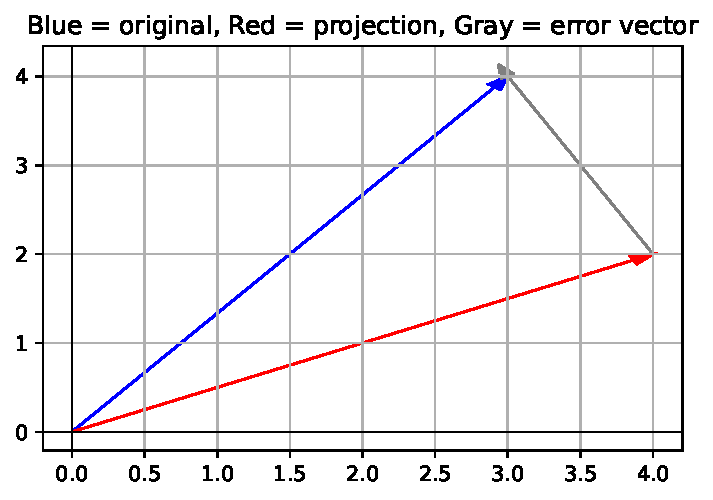
\includegraphics[keepaspectratio]{books/en-US/lab_files/figure-latex/cell-273-output-1.pdf}}

The projection is the closest point on the line to the original vector.

\begin{enumerate}
\def\labelenumi{\arabic{enumi}.}
\setcounter{enumi}{2}
\tightlist
\item
  Reflection across a line
\end{enumerate}

The reflection matrix across the line spanned by \(u\) is:

\[
R = 2P - I
\]

\begin{Shaded}
\begin{Highlighting}[]
\NormalTok{I }\OperatorTok{=}\NormalTok{ np.eye(}\DecValTok{2}\NormalTok{)}
\NormalTok{R }\OperatorTok{=} \DecValTok{2}\OperatorTok{*}\NormalTok{P }\OperatorTok{{-}}\NormalTok{ I}

\NormalTok{reflect\_v }\OperatorTok{=}\NormalTok{ R }\OperatorTok{@}\NormalTok{ v}
\BuiltInTok{print}\NormalTok{(}\StringTok{"Reflection of v across line u:"}\NormalTok{, reflect\_v)}
\end{Highlighting}
\end{Shaded}

\begin{verbatim}
Reflection of v across line u: [ 5.0000000e+00 -4.4408921e-16]
\end{verbatim}

\begin{enumerate}
\def\labelenumi{\arabic{enumi}.}
\setcounter{enumi}{3}
\tightlist
\item
  Checking algebraic properties
\end{enumerate}

\begin{itemize}
\tightlist
\item
  Projection: \(P^2 = P\) (idempotent).
\item
  Reflection: \(R^2 = I\) (involutive).
\end{itemize}

\begin{Shaded}
\begin{Highlighting}[]
\BuiltInTok{print}\NormalTok{(}\StringTok{"P\^{}2 =}\CharTok{\textbackslash{}n}\StringTok{"}\NormalTok{, P }\OperatorTok{@}\NormalTok{ P)}
\BuiltInTok{print}\NormalTok{(}\StringTok{"R\^{}2 =}\CharTok{\textbackslash{}n}\StringTok{"}\NormalTok{, R }\OperatorTok{@}\NormalTok{ R)}
\end{Highlighting}
\end{Shaded}

\begin{verbatim}
P^2 =
 [[0.8 0.4]
 [0.4 0.2]]
R^2 =
 [[ 1.00000000e+00 -1.59872116e-16]
 [-1.59872116e-16  1.00000000e+00]]
\end{verbatim}

\begin{enumerate}
\def\labelenumi{\arabic{enumi}.}
\setcounter{enumi}{4}
\tightlist
\item
  Projection in higher dimensions
\end{enumerate}

Project onto the plane spanned by two vectors in \(\mathbb{R}^3\).

\begin{Shaded}
\begin{Highlighting}[]
\NormalTok{u1 }\OperatorTok{=}\NormalTok{ np.array([}\DecValTok{1}\NormalTok{,}\DecValTok{0}\NormalTok{,}\DecValTok{0}\NormalTok{], dtype}\OperatorTok{=}\BuiltInTok{float}\NormalTok{)}
\NormalTok{u2 }\OperatorTok{=}\NormalTok{ np.array([}\DecValTok{0}\NormalTok{,}\DecValTok{1}\NormalTok{,}\DecValTok{0}\NormalTok{], dtype}\OperatorTok{=}\BuiltInTok{float}\NormalTok{)}

\NormalTok{U }\OperatorTok{=}\NormalTok{ np.column\_stack((u1,u2))   }\CommentTok{\# basis for plane}
\NormalTok{P\_plane }\OperatorTok{=}\NormalTok{ U }\OperatorTok{@}\NormalTok{ np.linalg.inv(U.T }\OperatorTok{@}\NormalTok{ U) }\OperatorTok{@}\NormalTok{ U.T}

\NormalTok{v }\OperatorTok{=}\NormalTok{ np.array([}\DecValTok{1}\NormalTok{,}\DecValTok{2}\NormalTok{,}\DecValTok{3}\NormalTok{], dtype}\OperatorTok{=}\BuiltInTok{float}\NormalTok{)}
\NormalTok{proj\_plane }\OperatorTok{=}\NormalTok{ P\_plane }\OperatorTok{@}\NormalTok{ v}
\BuiltInTok{print}\NormalTok{(}\StringTok{"Projection onto xy{-}plane:"}\NormalTok{, proj\_plane)}
\end{Highlighting}
\end{Shaded}

\begin{verbatim}
Projection onto xy-plane: [1. 2. 0.]
\end{verbatim}

\subsubsection{Try It Yourself}\label{try-it-yourself-145}

\begin{enumerate}
\def\labelenumi{\arabic{enumi}.}
\tightlist
\item
  Project \([4,5]\) onto the x-axis and verify the result.
\item
  Reflect \([1,2]\) across the line \(y=x\).
\item
  Create a random 3D vector and project it onto the plane spanned by
  \([1,1,0]\) and \([0,1,1]\).
\end{enumerate}

\subsubsection{The Takeaway}\label{the-takeaway-29}

\begin{itemize}
\tightlist
\item
  Projection: idempotent (\(P^2 = P\)), finds the closest vector in a
  subspace.
\item
  Reflection: involutive (\(R^2 = I\)), flips across a line/plane but
  preserves lengths.
\item
  Both are simple but powerful examples of linear transformations with
  clear geometry.
\end{itemize}

\subsection{48. Rotations and Shear (Geometric
Intuition)}\label{rotations-and-shear-geometric-intuition}

Two transformations often used in geometry, graphics, and physics are
rotations and shears. Both are linear maps, but they behave differently:

\begin{itemize}
\tightlist
\item
  Rotation preserves lengths and angles.
\item
  Shear preserves area (in 2D) but distorts shapes, turning squares into
  parallelograms.
\end{itemize}

\subsubsection{Set Up Your Lab}\label{set-up-your-lab-47}

\begin{Shaded}
\begin{Highlighting}[]
\ImportTok{import}\NormalTok{ numpy }\ImportTok{as}\NormalTok{ np}
\ImportTok{import}\NormalTok{ matplotlib.pyplot }\ImportTok{as}\NormalTok{ plt}
\end{Highlighting}
\end{Shaded}

\subsubsection{Step-by-Step Code
Walkthrough}\label{step-by-step-code-walkthrough-47}

\begin{enumerate}
\def\labelenumi{\arabic{enumi}.}
\tightlist
\item
  Rotation in 2D
\end{enumerate}

The rotation matrix by angle \(\theta\) is:

\[
R(\theta) = \begin{bmatrix} 
\cos\theta & -\sin\theta \\ 
\sin\theta & \cos\theta 
\end{bmatrix}
\]

\begin{Shaded}
\begin{Highlighting}[]
\KeywordTok{def}\NormalTok{ rotation\_matrix(theta):}
    \ControlFlowTok{return}\NormalTok{ np.array([}
\NormalTok{        [np.cos(theta), }\OperatorTok{{-}}\NormalTok{np.sin(theta)],}
\NormalTok{        [np.sin(theta),  np.cos(theta)]}
\NormalTok{    ])}

\NormalTok{theta }\OperatorTok{=}\NormalTok{ np.pi}\OperatorTok{/}\DecValTok{4}   \CommentTok{\# 45 degrees}
\NormalTok{R }\OperatorTok{=}\NormalTok{ rotation\_matrix(theta)}

\NormalTok{v }\OperatorTok{=}\NormalTok{ np.array([}\DecValTok{2}\NormalTok{,}\DecValTok{1}\NormalTok{])}
\NormalTok{rotated\_v }\OperatorTok{=}\NormalTok{ R }\OperatorTok{@}\NormalTok{ v}
\BuiltInTok{print}\NormalTok{(}\StringTok{"Original v:"}\NormalTok{, v)}
\BuiltInTok{print}\NormalTok{(}\StringTok{"Rotated v (45°):"}\NormalTok{, rotated\_v)}
\end{Highlighting}
\end{Shaded}

\begin{verbatim}
Original v: [2 1]
Rotated v (45°): [0.70710678 2.12132034]
\end{verbatim}

\begin{enumerate}
\def\labelenumi{\arabic{enumi}.}
\setcounter{enumi}{1}
\tightlist
\item
  Visualizing rotation
\end{enumerate}

\begin{Shaded}
\begin{Highlighting}[]
\NormalTok{plt.arrow(}\DecValTok{0}\NormalTok{,}\DecValTok{0}\NormalTok{,v[}\DecValTok{0}\NormalTok{],v[}\DecValTok{1}\NormalTok{],head\_width}\OperatorTok{=}\FloatTok{0.1}\NormalTok{,color}\OperatorTok{=}\StringTok{"blue"}\NormalTok{,length\_includes\_head}\OperatorTok{=}\VariableTok{True}\NormalTok{)}
\NormalTok{plt.arrow(}\DecValTok{0}\NormalTok{,}\DecValTok{0}\NormalTok{,rotated\_v[}\DecValTok{0}\NormalTok{],rotated\_v[}\DecValTok{1}\NormalTok{],head\_width}\OperatorTok{=}\FloatTok{0.1}\NormalTok{,color}\OperatorTok{=}\StringTok{"red"}\NormalTok{,length\_includes\_head}\OperatorTok{=}\VariableTok{True}\NormalTok{)}

\NormalTok{plt.axhline(}\DecValTok{0}\NormalTok{,color}\OperatorTok{=}\StringTok{\textquotesingle{}black\textquotesingle{}}\NormalTok{,linewidth}\OperatorTok{=}\FloatTok{0.5}\NormalTok{)}
\NormalTok{plt.axvline(}\DecValTok{0}\NormalTok{,color}\OperatorTok{=}\StringTok{\textquotesingle{}black\textquotesingle{}}\NormalTok{,linewidth}\OperatorTok{=}\FloatTok{0.5}\NormalTok{)}
\NormalTok{plt.grid()}
\NormalTok{plt.title(}\StringTok{"Blue = original, Red = rotated (45°)"}\NormalTok{)}
\NormalTok{plt.axis(}\StringTok{"equal"}\NormalTok{)}
\NormalTok{plt.show()}
\end{Highlighting}
\end{Shaded}

\pandocbounded{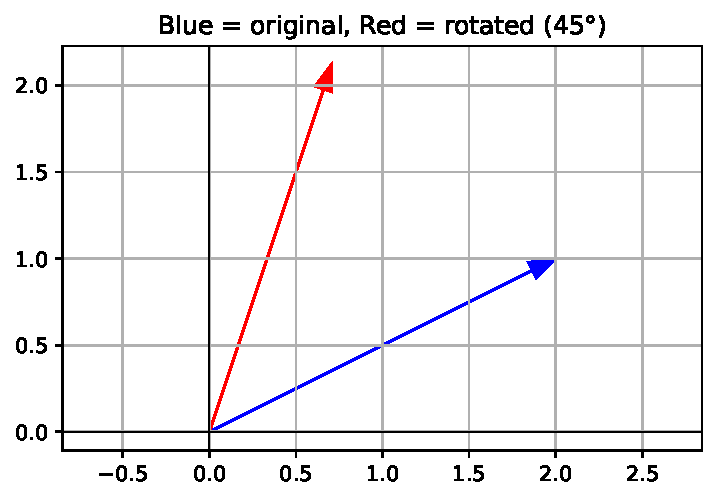
\includegraphics[keepaspectratio]{books/en-US/lab_files/figure-latex/cell-279-output-1.pdf}}

The vector rotates counterclockwise by 45°.

\begin{enumerate}
\def\labelenumi{\arabic{enumi}.}
\setcounter{enumi}{2}
\tightlist
\item
  Shear in 2D
\end{enumerate}

A shear along the x-axis by factor \(k\):

\[
S = \begin{bmatrix} 
1 & k \\ 
0 & 1 
\end{bmatrix}
\]

\begin{Shaded}
\begin{Highlighting}[]
\NormalTok{k }\OperatorTok{=} \FloatTok{1.0}
\NormalTok{S }\OperatorTok{=}\NormalTok{ np.array([}
\NormalTok{    [}\DecValTok{1}\NormalTok{,k],}
\NormalTok{    [}\DecValTok{0}\NormalTok{,}\DecValTok{1}\NormalTok{]}
\NormalTok{])}

\NormalTok{sheared\_v }\OperatorTok{=}\NormalTok{ S }\OperatorTok{@}\NormalTok{ v}
\BuiltInTok{print}\NormalTok{(}\StringTok{"Sheared v:"}\NormalTok{, sheared\_v)}
\end{Highlighting}
\end{Shaded}

\begin{verbatim}
Sheared v: [3. 1.]
\end{verbatim}

\begin{enumerate}
\def\labelenumi{\arabic{enumi}.}
\setcounter{enumi}{3}
\tightlist
\item
  Visualizing shear
\end{enumerate}

\begin{Shaded}
\begin{Highlighting}[]
\NormalTok{plt.arrow(}\DecValTok{0}\NormalTok{,}\DecValTok{0}\NormalTok{,v[}\DecValTok{0}\NormalTok{],v[}\DecValTok{1}\NormalTok{],head\_width}\OperatorTok{=}\FloatTok{0.1}\NormalTok{,color}\OperatorTok{=}\StringTok{"blue"}\NormalTok{,length\_includes\_head}\OperatorTok{=}\VariableTok{True}\NormalTok{)}
\NormalTok{plt.arrow(}\DecValTok{0}\NormalTok{,}\DecValTok{0}\NormalTok{,sheared\_v[}\DecValTok{0}\NormalTok{],sheared\_v[}\DecValTok{1}\NormalTok{],head\_width}\OperatorTok{=}\FloatTok{0.1}\NormalTok{,color}\OperatorTok{=}\StringTok{"green"}\NormalTok{,length\_includes\_head}\OperatorTok{=}\VariableTok{True}\NormalTok{)}

\NormalTok{plt.axhline(}\DecValTok{0}\NormalTok{,color}\OperatorTok{=}\StringTok{\textquotesingle{}black\textquotesingle{}}\NormalTok{,linewidth}\OperatorTok{=}\FloatTok{0.5}\NormalTok{)}
\NormalTok{plt.axvline(}\DecValTok{0}\NormalTok{,color}\OperatorTok{=}\StringTok{\textquotesingle{}black\textquotesingle{}}\NormalTok{,linewidth}\OperatorTok{=}\FloatTok{0.5}\NormalTok{)}
\NormalTok{plt.grid()}
\NormalTok{plt.title(}\StringTok{"Blue = original, Green = sheared"}\NormalTok{)}
\NormalTok{plt.axis(}\StringTok{"equal"}\NormalTok{)}
\NormalTok{plt.show()}
\end{Highlighting}
\end{Shaded}

\pandocbounded{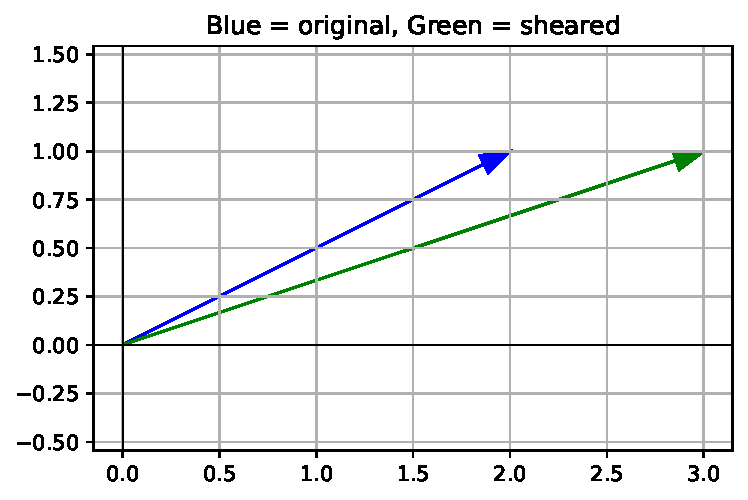
\includegraphics[keepaspectratio]{books/en-US/lab_files/figure-latex/cell-281-output-1.pdf}}

The shear moves the vector sideways, distorting its angle.

\begin{enumerate}
\def\labelenumi{\arabic{enumi}.}
\setcounter{enumi}{4}
\tightlist
\item
  Properties check
\end{enumerate}

\begin{itemize}
\tightlist
\item
  Rotation preserves length:
\end{itemize}

\begin{Shaded}
\begin{Highlighting}[]
\BuiltInTok{print}\NormalTok{(}\StringTok{"||v|| ="}\NormalTok{, np.linalg.norm(v))}
\BuiltInTok{print}\NormalTok{(}\StringTok{"||R v|| ="}\NormalTok{, np.linalg.norm(rotated\_v))}
\end{Highlighting}
\end{Shaded}

\begin{verbatim}
||v|| = 2.23606797749979
||R v|| = 2.2360679774997894
\end{verbatim}

\begin{itemize}
\tightlist
\item
  Shear preserves area (determinant = 1):
\end{itemize}

\begin{Shaded}
\begin{Highlighting}[]
\BuiltInTok{print}\NormalTok{(}\StringTok{"det(S) ="}\NormalTok{, np.linalg.det(S))}
\end{Highlighting}
\end{Shaded}

\begin{verbatim}
det(S) = 1.0
\end{verbatim}

\subsubsection{Try It Yourself}\label{try-it-yourself-146}

\begin{enumerate}
\def\labelenumi{\arabic{enumi}.}
\tightlist
\item
  Rotate \([1,0]\) by 90° and check it becomes \([0,1]\).
\item
  Apply shear with \(k=2\) to a square (points
  \((0,0),(1,0),(1,1),(0,1)\)) and plot before/after.
\item
  Combine rotation and shear: apply shear first, then rotation. What
  happens?
\end{enumerate}

\subsubsection{The Takeaway}\label{the-takeaway-30}

\begin{itemize}
\tightlist
\item
  Rotation: length- and angle-preserving, determinant = 1.
\item
  Shear: shape-distorting but area-preserving, determinant = 1.
\item
  Both are linear maps that provide geometric intuition and real-world
  modeling tools.
\end{itemize}

\subsection{49. Rank and Operator Viewpoint (Rank Beyond
Elimination)}\label{rank-and-operator-viewpoint-rank-beyond-elimination}

The rank of a matrix tells us how much ``information'' a linear map
carries. Algebraically, it is the dimension of the image (column space).
Geometrically, it measures how many independent directions survive the
transformation.

From the operator viewpoint:

\begin{itemize}
\tightlist
\item
  A matrix \(A\) is not just a table of numbers - it is a linear
  operator that maps vectors to other vectors.
\item
  The rank is the dimension of the output space that \(A\) actually
  reaches.
\end{itemize}

\subsubsection{Set Up Your Lab}\label{set-up-your-lab-48}

\begin{Shaded}
\begin{Highlighting}[]
\ImportTok{import}\NormalTok{ numpy }\ImportTok{as}\NormalTok{ np}
\ImportTok{from}\NormalTok{ sympy }\ImportTok{import}\NormalTok{ Matrix}
\end{Highlighting}
\end{Shaded}

\subsubsection{Step-by-Step Code
Walkthrough}\label{step-by-step-code-walkthrough-48}

\begin{enumerate}
\def\labelenumi{\arabic{enumi}.}
\tightlist
\item
  Rank via elimination (SymPy)
\end{enumerate}

\begin{Shaded}
\begin{Highlighting}[]
\NormalTok{A }\OperatorTok{=}\NormalTok{ Matrix([}
\NormalTok{    [}\DecValTok{1}\NormalTok{,}\DecValTok{2}\NormalTok{,}\DecValTok{3}\NormalTok{],}
\NormalTok{    [}\DecValTok{2}\NormalTok{,}\DecValTok{4}\NormalTok{,}\DecValTok{6}\NormalTok{],}
\NormalTok{    [}\DecValTok{1}\NormalTok{,}\DecValTok{1}\NormalTok{,}\DecValTok{1}\NormalTok{]}
\NormalTok{])}

\BuiltInTok{print}\NormalTok{(}\StringTok{"Matrix A:}\CharTok{\textbackslash{}n}\StringTok{"}\NormalTok{, A)}
\BuiltInTok{print}\NormalTok{(}\StringTok{"Rank of A:"}\NormalTok{, A.rank())}
\end{Highlighting}
\end{Shaded}

\begin{verbatim}
Matrix A:
 Matrix([[1, 2, 3], [2, 4, 6], [1, 1, 1]])
Rank of A: 2
\end{verbatim}

Here, the second row is a multiple of the first → less independence →
rank \textless{} 3.

\begin{enumerate}
\def\labelenumi{\arabic{enumi}.}
\setcounter{enumi}{1}
\tightlist
\item
  Rank via NumPy
\end{enumerate}

\begin{Shaded}
\begin{Highlighting}[]
\NormalTok{A\_np }\OperatorTok{=}\NormalTok{ np.array([[}\DecValTok{1}\NormalTok{,}\DecValTok{2}\NormalTok{,}\DecValTok{3}\NormalTok{],[}\DecValTok{2}\NormalTok{,}\DecValTok{4}\NormalTok{,}\DecValTok{6}\NormalTok{],[}\DecValTok{1}\NormalTok{,}\DecValTok{1}\NormalTok{,}\DecValTok{1}\NormalTok{]], dtype}\OperatorTok{=}\BuiltInTok{float}\NormalTok{)}
\BuiltInTok{print}\NormalTok{(}\StringTok{"Rank (NumPy):"}\NormalTok{, np.linalg.matrix\_rank(A\_np))}
\end{Highlighting}
\end{Shaded}

\begin{verbatim}
Rank (NumPy): 2
\end{verbatim}

\begin{enumerate}
\def\labelenumi{\arabic{enumi}.}
\setcounter{enumi}{2}
\tightlist
\item
  Operator viewpoint
\end{enumerate}

Let's apply \(A\) to random vectors:

\begin{Shaded}
\begin{Highlighting}[]
\ControlFlowTok{for}\NormalTok{ v }\KeywordTok{in}\NormalTok{ [np.array([}\DecValTok{1}\NormalTok{,}\DecValTok{0}\NormalTok{,}\DecValTok{0}\NormalTok{]), np.array([}\DecValTok{0}\NormalTok{,}\DecValTok{1}\NormalTok{,}\DecValTok{0}\NormalTok{]), np.array([}\DecValTok{0}\NormalTok{,}\DecValTok{0}\NormalTok{,}\DecValTok{1}\NormalTok{])]:}
    \BuiltInTok{print}\NormalTok{(}\StringTok{"A @"}\NormalTok{, v, }\StringTok{"="}\NormalTok{, A\_np }\OperatorTok{@}\NormalTok{ v)}
\end{Highlighting}
\end{Shaded}

\begin{verbatim}
A @ [1 0 0] = [1. 2. 1.]
A @ [0 1 0] = [2. 4. 1.]
A @ [0 0 1] = [3. 6. 1.]
\end{verbatim}

Even though we started in 3D, all outputs lie in a plane in
\(\mathbb{R}^3\). That's why rank = 2.

\begin{enumerate}
\def\labelenumi{\arabic{enumi}.}
\setcounter{enumi}{3}
\tightlist
\item
  Full rank vs reduced rank
\end{enumerate}

\begin{itemize}
\tightlist
\item
  Full rank: the transformation preserves dimension (no collapse).
\item
  Reduced rank: the transformation collapses onto a lower-dimensional
  subspace.
\end{itemize}

Example full-rank:

\begin{Shaded}
\begin{Highlighting}[]
\NormalTok{B }\OperatorTok{=}\NormalTok{ Matrix([}
\NormalTok{    [}\DecValTok{1}\NormalTok{,}\DecValTok{0}\NormalTok{,}\DecValTok{0}\NormalTok{],}
\NormalTok{    [}\DecValTok{0}\NormalTok{,}\DecValTok{1}\NormalTok{,}\DecValTok{0}\NormalTok{],}
\NormalTok{    [}\DecValTok{0}\NormalTok{,}\DecValTok{0}\NormalTok{,}\DecValTok{1}\NormalTok{]}
\NormalTok{])}

\BuiltInTok{print}\NormalTok{(}\StringTok{"Rank of B:"}\NormalTok{, B.rank())}
\end{Highlighting}
\end{Shaded}

\begin{verbatim}
Rank of B: 3
\end{verbatim}

\begin{enumerate}
\def\labelenumi{\arabic{enumi}.}
\setcounter{enumi}{4}
\tightlist
\item
  Connection to nullity
\end{enumerate}

The rank-nullity theorem:

\[
\text{rank}(A) + \text{nullity}(A) = \text{number of columns of } A
\]

Check with SymPy:

\begin{Shaded}
\begin{Highlighting}[]
\BuiltInTok{print}\NormalTok{(}\StringTok{"Null space (basis):"}\NormalTok{, A.nullspace())}
\BuiltInTok{print}\NormalTok{(}\StringTok{"Nullity:"}\NormalTok{, }\BuiltInTok{len}\NormalTok{(A.nullspace()))}
\BuiltInTok{print}\NormalTok{(}\StringTok{"Rank + Nullity ="}\NormalTok{, A.rank() }\OperatorTok{+} \BuiltInTok{len}\NormalTok{(A.nullspace()))}
\end{Highlighting}
\end{Shaded}

\begin{verbatim}
Null space (basis): [Matrix([
[ 1],
[-2],
[ 1]])]
Nullity: 1
Rank + Nullity = 3
\end{verbatim}

\subsubsection{Try It Yourself}\label{try-it-yourself-147}

\begin{enumerate}
\def\labelenumi{\arabic{enumi}.}
\item
  Take

  \[
  \begin{bmatrix} 1 & 1 \\ 1 & 1 \end{bmatrix}
  \]

  and compute its rank. Why is it 1?
\item
  For a random 4×4 matrix, use \texttt{np.linalg.matrix\_rank} to check
  if it's invertible.
\item
  Verify rank-nullity theorem for a 3×5 random integer matrix.
\end{enumerate}

\subsubsection{The Takeaway}\label{the-takeaway-31}

\begin{itemize}
\tightlist
\item
  Rank = dimension of the image (how many independent outputs a
  transformation has).
\item
  Operator viewpoint: rank shows how much of the input space survives
  after transformation.
\item
  Rank-nullity links the image and kernel - together they fully describe
  a linear operator.
\end{itemize}

\subsection{50. Block Matrices and Block Maps (Divide and Conquer
Structure)}\label{block-matrices-and-block-maps-divide-and-conquer-structure}

Sometimes matrices can be arranged in blocks (submatrices). Treating a
big matrix as smaller pieces helps simplify calculations, especially in
systems with structure (networks, coupled equations, or partitioned
variables).

\subsubsection{Set Up Your Lab}\label{set-up-your-lab-49}

\begin{Shaded}
\begin{Highlighting}[]
\ImportTok{import}\NormalTok{ numpy }\ImportTok{as}\NormalTok{ np}
\ImportTok{from}\NormalTok{ sympy }\ImportTok{import}\NormalTok{ Matrix}
\end{Highlighting}
\end{Shaded}

\subsubsection{Step-by-Step Code
Walkthrough}\label{step-by-step-code-walkthrough-49}

\begin{enumerate}
\def\labelenumi{\arabic{enumi}.}
\tightlist
\item
  Constructing block matrices
\end{enumerate}

We can build a block matrix from smaller pieces:

\begin{Shaded}
\begin{Highlighting}[]
\NormalTok{A11 }\OperatorTok{=}\NormalTok{ Matrix([[}\DecValTok{1}\NormalTok{,}\DecValTok{2}\NormalTok{],[}\DecValTok{3}\NormalTok{,}\DecValTok{4}\NormalTok{]])}
\NormalTok{A12 }\OperatorTok{=}\NormalTok{ Matrix([[}\DecValTok{5}\NormalTok{,}\DecValTok{6}\NormalTok{],[}\DecValTok{7}\NormalTok{,}\DecValTok{8}\NormalTok{]])}
\NormalTok{A21 }\OperatorTok{=}\NormalTok{ Matrix([[}\DecValTok{9}\NormalTok{,}\DecValTok{10}\NormalTok{]])}
\NormalTok{A22 }\OperatorTok{=}\NormalTok{ Matrix([[}\DecValTok{11}\NormalTok{,}\DecValTok{12}\NormalTok{]])}

\CommentTok{\# Combine into a block matrix}
\NormalTok{A }\OperatorTok{=}\NormalTok{ Matrix.vstack(}
\NormalTok{    Matrix.hstack(A11, A12),}
\NormalTok{    Matrix.hstack(A21, A22)}
\NormalTok{)}
\BuiltInTok{print}\NormalTok{(}\StringTok{"Block matrix A:}\CharTok{\textbackslash{}n}\StringTok{"}\NormalTok{, A)}
\end{Highlighting}
\end{Shaded}

\begin{verbatim}
Block matrix A:
 Matrix([[1, 2, 5, 6], [3, 4, 7, 8], [9, 10, 11, 12]])
\end{verbatim}

\begin{enumerate}
\def\labelenumi{\arabic{enumi}.}
\setcounter{enumi}{1}
\tightlist
\item
  Block multiplication
\end{enumerate}

If a matrix is partitioned into blocks, multiplication follows block
rules:

\[
\begin{bmatrix} A & B \\ C & D \end{bmatrix}
\begin{bmatrix} x \\ y \end{bmatrix}
= \begin{bmatrix} Ax + By \\ Cx + Dy \end{bmatrix}
\]

Example:

\begin{Shaded}
\begin{Highlighting}[]
\NormalTok{A }\OperatorTok{=}\NormalTok{ Matrix([}
\NormalTok{    [}\DecValTok{1}\NormalTok{,}\DecValTok{2}\NormalTok{,}\DecValTok{5}\NormalTok{,}\DecValTok{6}\NormalTok{],}
\NormalTok{    [}\DecValTok{3}\NormalTok{,}\DecValTok{4}\NormalTok{,}\DecValTok{7}\NormalTok{,}\DecValTok{8}\NormalTok{],}
\NormalTok{    [}\DecValTok{9}\NormalTok{,}\DecValTok{10}\NormalTok{,}\DecValTok{11}\NormalTok{,}\DecValTok{12}\NormalTok{]}
\NormalTok{])}

\NormalTok{x }\OperatorTok{=}\NormalTok{ Matrix([}\DecValTok{1}\NormalTok{,}\DecValTok{1}\NormalTok{,}\DecValTok{2}\NormalTok{,}\DecValTok{2}\NormalTok{])}
\BuiltInTok{print}\NormalTok{(}\StringTok{"A * x ="}\NormalTok{, A}\OperatorTok{*}\NormalTok{x)}
\end{Highlighting}
\end{Shaded}

\begin{verbatim}
A * x = Matrix([[25], [37], [65]])
\end{verbatim}

Here the vector is split into blocks \([x,y]\).

\begin{enumerate}
\def\labelenumi{\arabic{enumi}.}
\setcounter{enumi}{2}
\tightlist
\item
  Block diagonal matrices
\end{enumerate}

Block diagonal = independent subproblems:

\begin{Shaded}
\begin{Highlighting}[]
\NormalTok{B1 }\OperatorTok{=}\NormalTok{ Matrix([[}\DecValTok{2}\NormalTok{,}\DecValTok{0}\NormalTok{],[}\DecValTok{0}\NormalTok{,}\DecValTok{2}\NormalTok{]])}
\NormalTok{B2 }\OperatorTok{=}\NormalTok{ Matrix([[}\DecValTok{3}\NormalTok{,}\DecValTok{1}\NormalTok{],[}\DecValTok{0}\NormalTok{,}\DecValTok{3}\NormalTok{]])}

\NormalTok{BlockDiag }\OperatorTok{=}\NormalTok{ Matrix([}
\NormalTok{    [}\DecValTok{2}\NormalTok{,}\DecValTok{0}\NormalTok{,}\DecValTok{0}\NormalTok{,}\DecValTok{0}\NormalTok{],}
\NormalTok{    [}\DecValTok{0}\NormalTok{,}\DecValTok{2}\NormalTok{,}\DecValTok{0}\NormalTok{,}\DecValTok{0}\NormalTok{],}
\NormalTok{    [}\DecValTok{0}\NormalTok{,}\DecValTok{0}\NormalTok{,}\DecValTok{3}\NormalTok{,}\DecValTok{1}\NormalTok{],}
\NormalTok{    [}\DecValTok{0}\NormalTok{,}\DecValTok{0}\NormalTok{,}\DecValTok{0}\NormalTok{,}\DecValTok{3}\NormalTok{]}
\NormalTok{])}

\BuiltInTok{print}\NormalTok{(}\StringTok{"Block diagonal matrix:}\CharTok{\textbackslash{}n}\StringTok{"}\NormalTok{, BlockDiag)}
\end{Highlighting}
\end{Shaded}

\begin{verbatim}
Block diagonal matrix:
 Matrix([[2, 0, 0, 0], [0, 2, 0, 0], [0, 0, 3, 1], [0, 0, 0, 3]])
\end{verbatim}

Applying this matrix acts separately on each block - like running two
smaller transformations in parallel.

\begin{enumerate}
\def\labelenumi{\arabic{enumi}.}
\setcounter{enumi}{3}
\tightlist
\item
  Inverse of block diagonal
\end{enumerate}

The inverse of a block diagonal is just the block diagonal of inverses:

\begin{Shaded}
\begin{Highlighting}[]
\NormalTok{B1\_inv }\OperatorTok{=}\NormalTok{ B1.inv()}
\NormalTok{B2\_inv }\OperatorTok{=}\NormalTok{ B2.inv()}
\NormalTok{BlockDiagInv }\OperatorTok{=}\NormalTok{ Matrix([}
\NormalTok{    [B1\_inv[}\DecValTok{0}\NormalTok{,}\DecValTok{0}\NormalTok{],}\DecValTok{0}\NormalTok{,}\DecValTok{0}\NormalTok{,}\DecValTok{0}\NormalTok{],}
\NormalTok{    [}\DecValTok{0}\NormalTok{,B1\_inv[}\DecValTok{1}\NormalTok{,}\DecValTok{1}\NormalTok{],}\DecValTok{0}\NormalTok{,}\DecValTok{0}\NormalTok{],}
\NormalTok{    [}\DecValTok{0}\NormalTok{,}\DecValTok{0}\NormalTok{,B2\_inv[}\DecValTok{0}\NormalTok{,}\DecValTok{0}\NormalTok{],B2\_inv[}\DecValTok{0}\NormalTok{,}\DecValTok{1}\NormalTok{]],}
\NormalTok{    [}\DecValTok{0}\NormalTok{,}\DecValTok{0}\NormalTok{,B2\_inv[}\DecValTok{1}\NormalTok{,}\DecValTok{0}\NormalTok{],B2\_inv[}\DecValTok{1}\NormalTok{,}\DecValTok{1}\NormalTok{]]}
\NormalTok{])}
\BuiltInTok{print}\NormalTok{(}\StringTok{"Inverse block diag:}\CharTok{\textbackslash{}n}\StringTok{"}\NormalTok{, BlockDiagInv)}
\end{Highlighting}
\end{Shaded}

\begin{verbatim}
Inverse block diag:
 Matrix([[1/2, 0, 0, 0], [0, 1/2, 0, 0], [0, 0, 1/3, -1/9], [0, 0, 0, 1/3]])
\end{verbatim}

\begin{enumerate}
\def\labelenumi{\arabic{enumi}.}
\setcounter{enumi}{4}
\tightlist
\item
  Practical example - coupled equations
\end{enumerate}

Suppose we have two independent systems:

\begin{itemize}
\tightlist
\item
  System 1: \(Ax = b\)
\item
  System 2: \(Cy = d\)
\end{itemize}

We can represent both together:

\[
\begin{bmatrix} A & 0 \\ 0 & C \end{bmatrix}
\begin{bmatrix} x \\ y \end{bmatrix}
= \begin{bmatrix} b \\ d \end{bmatrix}
\]

This shows how block matrices organize multiple systems in one big
equation.

\subsubsection{Try It Yourself}\label{try-it-yourself-148}

\begin{enumerate}
\def\labelenumi{\arabic{enumi}.}
\tightlist
\item
  Build a block diagonal matrix with three 2×2 blocks. Apply it to a
  vector.
\item
  Verify block multiplication rule by manually computing \(Ax + By\) and
  \(Cx + Dy\).
\item
  Write two small systems of equations and combine them into one block
  system.
\end{enumerate}

\subsubsection{The Takeaway}\label{the-takeaway-32}

\begin{itemize}
\tightlist
\item
  Block matrices let us break down big systems into smaller parts.
\item
  Block diagonal matrices = independent subsystems.
\item
  Thinking in blocks simplifies algebra, programming, and numerical
  computation.
\end{itemize}

\section{Chapter 6. Determinants and
volume}\label{chapter-6.-determinants-and-volume-2}

\subsection{51. Areas, Volumes, and Signed Scale Factors (Geometric
Entry
Point)}\label{areas-volumes-and-signed-scale-factors-geometric-entry-point}

The determinant of a matrix has a deep geometric meaning: it tells us
how a linear transformation scales area (in 2D), volume (in 3D), or
higher-dimensional content. It can also flip orientation (sign).

\subsubsection{Set Up Your Lab}\label{set-up-your-lab-50}

\begin{Shaded}
\begin{Highlighting}[]
\ImportTok{import}\NormalTok{ numpy }\ImportTok{as}\NormalTok{ np}
\ImportTok{from}\NormalTok{ sympy }\ImportTok{import}\NormalTok{ Matrix}
\end{Highlighting}
\end{Shaded}

\subsubsection{Step-by-Step Code
Walkthrough}\label{step-by-step-code-walkthrough-50}

\begin{enumerate}
\def\labelenumi{\arabic{enumi}.}
\tightlist
\item
  Determinant in 2D (area scaling)
\end{enumerate}

Let's take a matrix that stretches and shears:

\begin{Shaded}
\begin{Highlighting}[]
\NormalTok{A }\OperatorTok{=}\NormalTok{ Matrix([}
\NormalTok{    [}\DecValTok{2}\NormalTok{,}\DecValTok{1}\NormalTok{],}
\NormalTok{    [}\DecValTok{1}\NormalTok{,}\DecValTok{1}\NormalTok{]}
\NormalTok{])}

\BuiltInTok{print}\NormalTok{(}\StringTok{"Determinant:"}\NormalTok{, A.det())}
\end{Highlighting}
\end{Shaded}

\begin{verbatim}
Determinant: 1
\end{verbatim}

The determinant = 1 → areas are preserved, even though the shape is
distorted.

\begin{enumerate}
\def\labelenumi{\arabic{enumi}.}
\setcounter{enumi}{1}
\tightlist
\item
  Unit square under transformation
\end{enumerate}

Transform the square with corners \((0,0),(1,0),(1,1),(0,1)\):

\begin{Shaded}
\begin{Highlighting}[]
\NormalTok{square }\OperatorTok{=}\NormalTok{ Matrix([}
\NormalTok{    [}\DecValTok{0}\NormalTok{,}\DecValTok{0}\NormalTok{],}
\NormalTok{    [}\DecValTok{1}\NormalTok{,}\DecValTok{0}\NormalTok{],}
\NormalTok{    [}\DecValTok{1}\NormalTok{,}\DecValTok{1}\NormalTok{],}
\NormalTok{    [}\DecValTok{0}\NormalTok{,}\DecValTok{1}\NormalTok{]}
\NormalTok{])}

\NormalTok{transformed }\OperatorTok{=}\NormalTok{ (A }\OperatorTok{*}\NormalTok{ square.T).T}
\BuiltInTok{print}\NormalTok{(}\StringTok{"Original square:}\CharTok{\textbackslash{}n}\StringTok{"}\NormalTok{, square)}
\BuiltInTok{print}\NormalTok{(}\StringTok{"Transformed square:}\CharTok{\textbackslash{}n}\StringTok{"}\NormalTok{, transformed)}
\end{Highlighting}
\end{Shaded}

\begin{verbatim}
Original square:
 Matrix([[0, 0], [1, 0], [1, 1], [0, 1]])
Transformed square:
 Matrix([[0, 0], [2, 1], [3, 2], [1, 1]])
\end{verbatim}

The area of the transformed shape equals \(|\det(A)|\).

\begin{enumerate}
\def\labelenumi{\arabic{enumi}.}
\setcounter{enumi}{2}
\tightlist
\item
  Determinant in 3D (volume scaling)
\end{enumerate}

\begin{Shaded}
\begin{Highlighting}[]
\NormalTok{B }\OperatorTok{=}\NormalTok{ Matrix([}
\NormalTok{    [}\DecValTok{1}\NormalTok{,}\DecValTok{2}\NormalTok{,}\DecValTok{0}\NormalTok{],}
\NormalTok{    [}\DecValTok{0}\NormalTok{,}\DecValTok{1}\NormalTok{,}\DecValTok{0}\NormalTok{],}
\NormalTok{    [}\DecValTok{0}\NormalTok{,}\DecValTok{0}\NormalTok{,}\DecValTok{3}\NormalTok{]}
\NormalTok{])}

\BuiltInTok{print}\NormalTok{(}\StringTok{"Determinant:"}\NormalTok{, B.det())}
\end{Highlighting}
\end{Shaded}

\begin{verbatim}
Determinant: 3
\end{verbatim}

\(\det(B)=3\) means that volumes are scaled by 3.

\begin{enumerate}
\def\labelenumi{\arabic{enumi}.}
\setcounter{enumi}{3}
\tightlist
\item
  Negative determinant = orientation flip
\end{enumerate}

\begin{Shaded}
\begin{Highlighting}[]
\NormalTok{C }\OperatorTok{=}\NormalTok{ Matrix([}
\NormalTok{    [}\DecValTok{0}\NormalTok{,}\DecValTok{1}\NormalTok{],}
\NormalTok{    [}\DecValTok{1}\NormalTok{,}\DecValTok{0}\NormalTok{]}
\NormalTok{])}

\BuiltInTok{print}\NormalTok{(}\StringTok{"Determinant:"}\NormalTok{, C.det())}
\end{Highlighting}
\end{Shaded}

\begin{verbatim}
Determinant: -1
\end{verbatim}

The determinant = -1 → area preserved but orientation flipped (like a
mirror reflection).

\begin{enumerate}
\def\labelenumi{\arabic{enumi}.}
\setcounter{enumi}{4}
\tightlist
\item
  NumPy version
\end{enumerate}

\begin{Shaded}
\begin{Highlighting}[]
\NormalTok{A }\OperatorTok{=}\NormalTok{ np.array([[}\DecValTok{2}\NormalTok{,}\DecValTok{1}\NormalTok{],[}\DecValTok{1}\NormalTok{,}\DecValTok{1}\NormalTok{]], dtype}\OperatorTok{=}\BuiltInTok{float}\NormalTok{)}
\BuiltInTok{print}\NormalTok{(}\StringTok{"Det (NumPy):"}\NormalTok{, np.linalg.det(A))}
\end{Highlighting}
\end{Shaded}

\begin{verbatim}
Det (NumPy): 1.0
\end{verbatim}

\subsubsection{Try It Yourself}\label{try-it-yourself-149}

\begin{enumerate}
\def\labelenumi{\arabic{enumi}.}
\item
  Take

  \[
  \begin{bmatrix} 3 & 0 \\ 0 & 2 \end{bmatrix}
  \]

  and compute the determinant. Verify it scales areas by 6.
\item
  Build a 3×3 shear matrix and check how it affects volume.
\item
  Test a reflection matrix and confirm that the determinant is negative.
\end{enumerate}

\subsubsection{The Takeaway}\label{the-takeaway-33}

\begin{itemize}
\tightlist
\item
  Determinant measures how a linear map scales area, volume, or
  hypervolume.
\item
  Positive determinant = preserves orientation; negative = flips it.
\item
  Magnitude of determinant = scaling factor of geometric content.
\end{itemize}

\subsection{52. Determinant via Linear Rules (Multilinearity, Sign,
Normalization)}\label{determinant-via-linear-rules-multilinearity-sign-normalization}

The determinant isn't just a formula; it's defined by three elegant
rules that make it unique. These rules capture its geometric meaning as
a volume-scaling factor.

\begin{enumerate}
\def\labelenumi{\arabic{enumi}.}
\tightlist
\item
  Multilinearity: Linear in each row (or column).
\item
  Sign Change: Swapping two rows flips the sign.
\item
  Normalization: The determinant of the identity matrix is 1.
\end{enumerate}

\subsubsection{Set Up Your Lab}\label{set-up-your-lab-51}

\begin{Shaded}
\begin{Highlighting}[]
\ImportTok{import}\NormalTok{ numpy }\ImportTok{as}\NormalTok{ np}
\ImportTok{from}\NormalTok{ sympy }\ImportTok{import}\NormalTok{ Matrix}
\end{Highlighting}
\end{Shaded}

\subsubsection{Step-by-Step Code
Walkthrough}\label{step-by-step-code-walkthrough-51}

\begin{enumerate}
\def\labelenumi{\arabic{enumi}.}
\tightlist
\item
  Multilinearity
\end{enumerate}

If one row is scaled, the determinant scales the same way.

\begin{Shaded}
\begin{Highlighting}[]
\NormalTok{A }\OperatorTok{=}\NormalTok{ Matrix([[}\DecValTok{1}\NormalTok{,}\DecValTok{2}\NormalTok{],[}\DecValTok{3}\NormalTok{,}\DecValTok{4}\NormalTok{]])}
\BuiltInTok{print}\NormalTok{(}\StringTok{"det(A):"}\NormalTok{, A.det())}

\NormalTok{B }\OperatorTok{=}\NormalTok{ Matrix([[}\DecValTok{2}\NormalTok{,}\DecValTok{4}\NormalTok{],[}\DecValTok{3}\NormalTok{,}\DecValTok{4}\NormalTok{]])  }\CommentTok{\# first row doubled}
\BuiltInTok{print}\NormalTok{(}\StringTok{"det(B):"}\NormalTok{, B.det())}
\end{Highlighting}
\end{Shaded}

\begin{verbatim}
det(A): -2
det(B): -4
\end{verbatim}

You'll see \texttt{det(B)\ =\ 2\ *\ det(A)}.

\begin{enumerate}
\def\labelenumi{\arabic{enumi}.}
\setcounter{enumi}{1}
\tightlist
\item
  Sign change by row swap
\end{enumerate}

\begin{Shaded}
\begin{Highlighting}[]
\NormalTok{C }\OperatorTok{=}\NormalTok{ Matrix([[}\DecValTok{1}\NormalTok{,}\DecValTok{2}\NormalTok{],[}\DecValTok{3}\NormalTok{,}\DecValTok{4}\NormalTok{]])}
\NormalTok{C\_swapped }\OperatorTok{=}\NormalTok{ Matrix([[}\DecValTok{3}\NormalTok{,}\DecValTok{4}\NormalTok{],[}\DecValTok{1}\NormalTok{,}\DecValTok{2}\NormalTok{]])}

\BuiltInTok{print}\NormalTok{(}\StringTok{"det(C):"}\NormalTok{, C.det())}
\BuiltInTok{print}\NormalTok{(}\StringTok{"det(C\_swapped):"}\NormalTok{, C\_swapped.det())}
\end{Highlighting}
\end{Shaded}

\begin{verbatim}
det(C): -2
det(C_swapped): 2
\end{verbatim}

Swapping rows flips the sign of the determinant.

\begin{enumerate}
\def\labelenumi{\arabic{enumi}.}
\setcounter{enumi}{2}
\tightlist
\item
  Normalization rule
\end{enumerate}

\begin{Shaded}
\begin{Highlighting}[]
\NormalTok{I }\OperatorTok{=}\NormalTok{ Matrix.eye(}\DecValTok{3}\NormalTok{)}
\BuiltInTok{print}\NormalTok{(}\StringTok{"det(I):"}\NormalTok{, I.det())}
\end{Highlighting}
\end{Shaded}

\begin{verbatim}
det(I): 1
\end{verbatim}

The determinant of the identity is always 1 - this fixes the scaling
baseline.

\begin{enumerate}
\def\labelenumi{\arabic{enumi}.}
\setcounter{enumi}{3}
\tightlist
\item
  Combining rules (example in 3×3)
\end{enumerate}

\begin{Shaded}
\begin{Highlighting}[]
\NormalTok{M }\OperatorTok{=}\NormalTok{ Matrix([[}\DecValTok{1}\NormalTok{,}\DecValTok{2}\NormalTok{,}\DecValTok{3}\NormalTok{],[}\DecValTok{4}\NormalTok{,}\DecValTok{5}\NormalTok{,}\DecValTok{6}\NormalTok{],[}\DecValTok{7}\NormalTok{,}\DecValTok{8}\NormalTok{,}\DecValTok{9}\NormalTok{]])}
\BuiltInTok{print}\NormalTok{(}\StringTok{"det(M):"}\NormalTok{, M.det())}
\end{Highlighting}
\end{Shaded}

\begin{verbatim}
det(M): 0
\end{verbatim}

Here, rows are linearly dependent, so the determinant is 0 - consistent
with multilinearity (since one row can be written as a combo of others).

\begin{enumerate}
\def\labelenumi{\arabic{enumi}.}
\setcounter{enumi}{4}
\tightlist
\item
  NumPy check
\end{enumerate}

\begin{Shaded}
\begin{Highlighting}[]
\NormalTok{A }\OperatorTok{=}\NormalTok{ np.array([[}\DecValTok{1}\NormalTok{,}\DecValTok{2}\NormalTok{],[}\DecValTok{3}\NormalTok{,}\DecValTok{4}\NormalTok{]], dtype}\OperatorTok{=}\BuiltInTok{float}\NormalTok{)}
\BuiltInTok{print}\NormalTok{(}\StringTok{"det(A) NumPy:"}\NormalTok{, np.linalg.det(A))}
\end{Highlighting}
\end{Shaded}

\begin{verbatim}
det(A) NumPy: -2.0000000000000004
\end{verbatim}

Both SymPy and NumPy confirm the same result.

\subsubsection{Try It Yourself}\label{try-it-yourself-150}

\begin{enumerate}
\def\labelenumi{\arabic{enumi}.}
\tightlist
\item
  Scale a row of a 3×3 matrix by 3. Confirm the determinant scales by 3.
\item
  Swap two rows twice in a row - does the determinant return to its
  original value?
\item
  Compute determinant of a triangular matrix. What pattern do you see?
\end{enumerate}

\subsubsection{The Takeaway}\label{the-takeaway-34}

\begin{itemize}
\tightlist
\item
  Determinant is defined by multilinearity, sign change, and
  normalization.
\item
  These rules uniquely pin down the determinant's behavior.
\item
  Every formula (cofactor expansion, row-reduction method, etc.) comes
  from these core principles.
\end{itemize}

\subsection{53. Determinant and Row Operations (How Each Move Changes
det)}\label{determinant-and-row-operations-how-each-move-changes-det}

Row operations are at the heart of Gaussian elimination, and the
determinant has simple, predictable reactions to them. Understanding
these reactions gives both computational shortcuts and geometric
intuition.

\subsubsection{The Three Key Rules}\label{the-three-key-rules}

\begin{enumerate}
\def\labelenumi{\arabic{enumi}.}
\tightlist
\item
  Row swap: Swapping two rows flips the sign of the determinant.
\item
  Row scaling: Multiplying a row by a scalar \(c\) multiplies the
  determinant by \(c\).
\item
  Row replacement: Adding a multiple of one row to another leaves the
  determinant unchanged.
\end{enumerate}

\subsubsection{Set Up Your Lab}\label{set-up-your-lab-52}

\begin{Shaded}
\begin{Highlighting}[]
\ImportTok{import}\NormalTok{ numpy }\ImportTok{as}\NormalTok{ np}
\ImportTok{from}\NormalTok{ sympy }\ImportTok{import}\NormalTok{ Matrix}
\end{Highlighting}
\end{Shaded}

\subsubsection{Step-by-Step Code
Walkthrough}\label{step-by-step-code-walkthrough-52}

\begin{enumerate}
\def\labelenumi{\arabic{enumi}.}
\tightlist
\item
  Row swap
\end{enumerate}

\begin{Shaded}
\begin{Highlighting}[]
\NormalTok{A }\OperatorTok{=}\NormalTok{ Matrix([[}\DecValTok{1}\NormalTok{,}\DecValTok{2}\NormalTok{],[}\DecValTok{3}\NormalTok{,}\DecValTok{4}\NormalTok{]])}
\BuiltInTok{print}\NormalTok{(}\StringTok{"det(A):"}\NormalTok{, A.det())}

\NormalTok{A\_swapped }\OperatorTok{=}\NormalTok{ Matrix([[}\DecValTok{3}\NormalTok{,}\DecValTok{4}\NormalTok{],[}\DecValTok{1}\NormalTok{,}\DecValTok{2}\NormalTok{]])}
\BuiltInTok{print}\NormalTok{(}\StringTok{"det(after swap):"}\NormalTok{, A\_swapped.det())}
\end{Highlighting}
\end{Shaded}

\begin{verbatim}
det(A): -2
det(after swap): 2
\end{verbatim}

The result flips sign.

\begin{enumerate}
\def\labelenumi{\arabic{enumi}.}
\setcounter{enumi}{1}
\tightlist
\item
  Row scaling
\end{enumerate}

\begin{Shaded}
\begin{Highlighting}[]
\NormalTok{B }\OperatorTok{=}\NormalTok{ Matrix([[}\DecValTok{1}\NormalTok{,}\DecValTok{2}\NormalTok{],[}\DecValTok{3}\NormalTok{,}\DecValTok{4}\NormalTok{]])}
\NormalTok{B\_scaled }\OperatorTok{=}\NormalTok{ Matrix([[}\DecValTok{2}\NormalTok{,}\DecValTok{4}\NormalTok{],[}\DecValTok{3}\NormalTok{,}\DecValTok{4}\NormalTok{]])  }\CommentTok{\# first row × 2}

\BuiltInTok{print}\NormalTok{(}\StringTok{"det(B):"}\NormalTok{, B.det())}
\BuiltInTok{print}\NormalTok{(}\StringTok{"det(after scaling row 1 by 2):"}\NormalTok{, B\_scaled.det())}
\end{Highlighting}
\end{Shaded}

\begin{verbatim}
det(B): -2
det(after scaling row 1 by 2): -4
\end{verbatim}

Determinant is multiplied by 2.

\begin{enumerate}
\def\labelenumi{\arabic{enumi}.}
\setcounter{enumi}{2}
\tightlist
\item
  Row replacement (no change)
\end{enumerate}

\begin{Shaded}
\begin{Highlighting}[]
\NormalTok{C }\OperatorTok{=}\NormalTok{ Matrix([[}\DecValTok{1}\NormalTok{,}\DecValTok{2}\NormalTok{],[}\DecValTok{3}\NormalTok{,}\DecValTok{4}\NormalTok{]])}
\NormalTok{C\_replaced }\OperatorTok{=}\NormalTok{ Matrix([[}\DecValTok{1}\NormalTok{,}\DecValTok{2}\NormalTok{],[}\DecValTok{3}\OperatorTok{{-}}\DecValTok{2}\OperatorTok{*}\DecValTok{1}\NormalTok{, }\DecValTok{4}\OperatorTok{{-}}\DecValTok{2}\OperatorTok{*}\DecValTok{2}\NormalTok{]])  }\CommentTok{\# row2 → row2 {-} 2*row1}

\BuiltInTok{print}\NormalTok{(}\StringTok{"det(C):"}\NormalTok{, C.det())}
\BuiltInTok{print}\NormalTok{(}\StringTok{"det(after row replacement):"}\NormalTok{, C\_replaced.det())}
\end{Highlighting}
\end{Shaded}

\begin{verbatim}
det(C): -2
det(after row replacement): -2
\end{verbatim}

Determinant stays the same.

\begin{enumerate}
\def\labelenumi{\arabic{enumi}.}
\setcounter{enumi}{3}
\tightlist
\item
  Triangular form shortcut
\end{enumerate}

Since elimination only uses row replacement (which doesn't change the
determinant) and row swaps/scales (which we can track), the determinant
of a triangular matrix is just the product of its diagonal entries.

\begin{Shaded}
\begin{Highlighting}[]
\NormalTok{D }\OperatorTok{=}\NormalTok{ Matrix([[}\DecValTok{2}\NormalTok{,}\DecValTok{1}\NormalTok{,}\DecValTok{3}\NormalTok{],[}\DecValTok{0}\NormalTok{,}\DecValTok{4}\NormalTok{,}\DecValTok{5}\NormalTok{],[}\DecValTok{0}\NormalTok{,}\DecValTok{0}\NormalTok{,}\DecValTok{6}\NormalTok{]])}
\BuiltInTok{print}\NormalTok{(}\StringTok{"det(D):"}\NormalTok{, D.det())}
\BuiltInTok{print}\NormalTok{(}\StringTok{"Product of diagonals:"}\NormalTok{, }\DecValTok{2}\OperatorTok{*}\DecValTok{4}\OperatorTok{*}\DecValTok{6}\NormalTok{)}
\end{Highlighting}
\end{Shaded}

\begin{verbatim}
det(D): 48
Product of diagonals: 48
\end{verbatim}

\begin{enumerate}
\def\labelenumi{\arabic{enumi}.}
\setcounter{enumi}{4}
\tightlist
\item
  NumPy confirmation
\end{enumerate}

\begin{Shaded}
\begin{Highlighting}[]
\NormalTok{A }\OperatorTok{=}\NormalTok{ np.array([[}\DecValTok{1}\NormalTok{,}\DecValTok{2}\NormalTok{,}\DecValTok{3}\NormalTok{],[}\DecValTok{0}\NormalTok{,}\DecValTok{4}\NormalTok{,}\DecValTok{5}\NormalTok{],[}\DecValTok{1}\NormalTok{,}\DecValTok{0}\NormalTok{,}\DecValTok{6}\NormalTok{]], dtype}\OperatorTok{=}\BuiltInTok{float}\NormalTok{)}
\BuiltInTok{print}\NormalTok{(}\StringTok{"det(A):"}\NormalTok{, np.linalg.det(A))}
\end{Highlighting}
\end{Shaded}

\begin{verbatim}
det(A): 22.000000000000004
\end{verbatim}

\subsubsection{Try It Yourself}\label{try-it-yourself-151}

\begin{enumerate}
\def\labelenumi{\arabic{enumi}.}
\item
  Take

  \[
  \begin{bmatrix} 2 & 3 \\ 4 & 6 \end{bmatrix}
  \]

  and scale the second row by \(\tfrac{1}{2}\). Compare determinants
  before and after.
\item
  Do Gaussian elimination on a 3×3 matrix, and track how each row
  operation changes the determinant.
\item
  Compute determinant by reducing to triangular form and compare with
  SymPy's \texttt{.det()}.
\end{enumerate}

\subsubsection{The Takeaway}\label{the-takeaway-35}

\begin{itemize}
\tightlist
\item
  Determinant reacts predictably to row operations.
\item
  Row replacement is ``safe'' (no change), scaling multiplies by the
  factor, and swapping flips the sign.
\item
  This makes elimination not just a solving tool, but also a method to
  compute determinants efficiently.
\end{itemize}

\subsection{54. Triangular Matrices and Product of Diagonals (Fast
Wins)}\label{triangular-matrices-and-product-of-diagonals-fast-wins}

For triangular matrices (upper or lower), the determinant is simply the
product of the diagonal entries. This rule is one of the biggest
shortcuts in linear algebra - no expansion or elimination needed.

\subsubsection{Why It Works}\label{why-it-works-2}

\begin{itemize}
\tightlist
\item
  Triangular matrices already look like the end result of Gaussian
  elimination.
\item
  Since row replacement operations don't change the determinant, what's
  left is just the product of the diagonal.
\end{itemize}

\subsubsection{Set Up Your Lab}\label{set-up-your-lab-53}

\begin{Shaded}
\begin{Highlighting}[]
\ImportTok{import}\NormalTok{ numpy }\ImportTok{as}\NormalTok{ np}
\ImportTok{from}\NormalTok{ sympy }\ImportTok{import}\NormalTok{ Matrix}
\end{Highlighting}
\end{Shaded}

\subsubsection{Step-by-Step Code
Walkthrough}\label{step-by-step-code-walkthrough-53}

\begin{enumerate}
\def\labelenumi{\arabic{enumi}.}
\tightlist
\item
  Upper triangular example
\end{enumerate}

\begin{Shaded}
\begin{Highlighting}[]
\NormalTok{A }\OperatorTok{=}\NormalTok{ Matrix([}
\NormalTok{    [}\DecValTok{2}\NormalTok{,}\DecValTok{1}\NormalTok{,}\DecValTok{3}\NormalTok{],}
\NormalTok{    [}\DecValTok{0}\NormalTok{,}\DecValTok{4}\NormalTok{,}\DecValTok{5}\NormalTok{],}
\NormalTok{    [}\DecValTok{0}\NormalTok{,}\DecValTok{0}\NormalTok{,}\DecValTok{6}\NormalTok{]}
\NormalTok{])}

\BuiltInTok{print}\NormalTok{(}\StringTok{"det(A):"}\NormalTok{, A.det())}
\BuiltInTok{print}\NormalTok{(}\StringTok{"Product of diagonals:"}\NormalTok{, }\DecValTok{2}\OperatorTok{*}\DecValTok{4}\OperatorTok{*}\DecValTok{6}\NormalTok{)}
\end{Highlighting}
\end{Shaded}

\begin{verbatim}
det(A): 48
Product of diagonals: 48
\end{verbatim}

Both values match exactly.

\begin{enumerate}
\def\labelenumi{\arabic{enumi}.}
\setcounter{enumi}{1}
\tightlist
\item
  Lower triangular example
\end{enumerate}

\begin{Shaded}
\begin{Highlighting}[]
\NormalTok{B }\OperatorTok{=}\NormalTok{ Matrix([}
\NormalTok{    [}\DecValTok{7}\NormalTok{,}\DecValTok{0}\NormalTok{,}\DecValTok{0}\NormalTok{],}
\NormalTok{    [}\DecValTok{2}\NormalTok{,}\DecValTok{5}\NormalTok{,}\DecValTok{0}\NormalTok{],}
\NormalTok{    [}\DecValTok{3}\NormalTok{,}\DecValTok{4}\NormalTok{,}\DecValTok{9}\NormalTok{]}
\NormalTok{])}

\BuiltInTok{print}\NormalTok{(}\StringTok{"det(B):"}\NormalTok{, B.det())}
\BuiltInTok{print}\NormalTok{(}\StringTok{"Product of diagonals:"}\NormalTok{, }\DecValTok{7}\OperatorTok{*}\DecValTok{5}\OperatorTok{*}\DecValTok{9}\NormalTok{)}
\end{Highlighting}
\end{Shaded}

\begin{verbatim}
det(B): 315
Product of diagonals: 315
\end{verbatim}

\begin{enumerate}
\def\labelenumi{\arabic{enumi}.}
\setcounter{enumi}{2}
\tightlist
\item
  Diagonal matrix (special case)
\end{enumerate}

For diagonal matrices, determinant = product of diagonal entries
directly.

\begin{Shaded}
\begin{Highlighting}[]
\NormalTok{C }\OperatorTok{=}\NormalTok{ Matrix.diag(}\DecValTok{3}\NormalTok{,}\DecValTok{5}\NormalTok{,}\DecValTok{7}\NormalTok{)}
\BuiltInTok{print}\NormalTok{(}\StringTok{"det(C):"}\NormalTok{, C.det())}
\BuiltInTok{print}\NormalTok{(}\StringTok{"Product of diagonals:"}\NormalTok{, }\DecValTok{3}\OperatorTok{*}\DecValTok{5}\OperatorTok{*}\DecValTok{7}\NormalTok{)}
\end{Highlighting}
\end{Shaded}

\begin{verbatim}
det(C): 105
Product of diagonals: 105
\end{verbatim}

\begin{enumerate}
\def\labelenumi{\arabic{enumi}.}
\setcounter{enumi}{3}
\tightlist
\item
  NumPy version
\end{enumerate}

\begin{Shaded}
\begin{Highlighting}[]
\NormalTok{A }\OperatorTok{=}\NormalTok{ np.array([[}\DecValTok{2}\NormalTok{,}\DecValTok{1}\NormalTok{,}\DecValTok{3}\NormalTok{],[}\DecValTok{0}\NormalTok{,}\DecValTok{4}\NormalTok{,}\DecValTok{5}\NormalTok{],[}\DecValTok{0}\NormalTok{,}\DecValTok{0}\NormalTok{,}\DecValTok{6}\NormalTok{]], dtype}\OperatorTok{=}\BuiltInTok{float}\NormalTok{)}
\BuiltInTok{print}\NormalTok{(}\StringTok{"det(A):"}\NormalTok{, np.linalg.det(A))}
\BuiltInTok{print}\NormalTok{(}\StringTok{"Product of diagonals:"}\NormalTok{, np.prod(np.diag(A)))}
\end{Highlighting}
\end{Shaded}

\begin{verbatim}
det(A): 47.999999999999986
Product of diagonals: 48.0
\end{verbatim}

\begin{enumerate}
\def\labelenumi{\arabic{enumi}.}
\setcounter{enumi}{4}
\tightlist
\item
  Quick elimination to triangular form
\end{enumerate}

Even for non-triangular matrices, elimination reduces them to triangular
form, where this rule applies.

\begin{Shaded}
\begin{Highlighting}[]
\NormalTok{D }\OperatorTok{=}\NormalTok{ Matrix([[}\DecValTok{1}\NormalTok{,}\DecValTok{2}\NormalTok{,}\DecValTok{3}\NormalTok{],[}\DecValTok{4}\NormalTok{,}\DecValTok{5}\NormalTok{,}\DecValTok{6}\NormalTok{],[}\DecValTok{7}\NormalTok{,}\DecValTok{8}\NormalTok{,}\DecValTok{10}\NormalTok{]])}
\BuiltInTok{print}\NormalTok{(}\StringTok{"det(D) via SymPy:"}\NormalTok{, D.det())}
\BuiltInTok{print}\NormalTok{(}\StringTok{"det(D) via LU decomposition:"}\NormalTok{, D.LUdecomposition()[}\DecValTok{0}\NormalTok{].det() }\OperatorTok{*}\NormalTok{ D.LUdecomposition()[}\DecValTok{1}\NormalTok{].det())}
\end{Highlighting}
\end{Shaded}

\begin{verbatim}
det(D) via SymPy: -3
det(D) via LU decomposition: -3
\end{verbatim}

\subsubsection{Try It Yourself}\label{try-it-yourself-152}

\begin{enumerate}
\def\labelenumi{\arabic{enumi}.}
\tightlist
\item
  Compute the determinant of a 4×4 diagonal matrix quickly.
\item
  Verify that triangular matrices with a zero on the diagonal always
  have determinant 0.
\item
  Use SymPy to check that elimination to triangular form preserves
  determinant (except for swaps/scales).
\end{enumerate}

\subsubsection{The Takeaway}\label{the-takeaway-36}

\begin{itemize}
\item
  For triangular (and diagonal) matrices:

  \[
  \det(A) = \prod_{i} a_{ii}
  \]
\item
  This shortcut makes determinant computation trivial.
\item
  Gaussian elimination leverages this fact: once reduced to triangular
  form, the determinant is just the product of pivots (with sign
  adjustments for swaps).
\end{itemize}

\subsection{55. det(AB) = det(A)det(B) (Multiplicative
Magic)}\label{detab-detadetb-multiplicative-magic}

One of the most elegant properties of determinants is multiplicativity:

\[
\det(AB) = \det(A)\,\det(B)
\]

This rule is powerful because it connects algebra (matrix
multiplication) with geometry (volume scaling).

\subsubsection{Geometric Intuition}\label{geometric-intuition-9}

\begin{itemize}
\tightlist
\item
  If \(A\) scales volumes by factor \(\det(A)\), and \(B\) scales them
  by \(\det(B)\), then applying \(B\) followed by \(A\) scales volumes
  by \(\det(A)\det(B)\).
\item
  This property works in all dimensions.
\end{itemize}

\subsubsection{Set Up Your Lab}\label{set-up-your-lab-54}

\begin{Shaded}
\begin{Highlighting}[]
\ImportTok{import}\NormalTok{ numpy }\ImportTok{as}\NormalTok{ np}
\ImportTok{from}\NormalTok{ sympy }\ImportTok{import}\NormalTok{ Matrix}
\end{Highlighting}
\end{Shaded}

\subsubsection{Step-by-Step Code
Walkthrough}\label{step-by-step-code-walkthrough-54}

\begin{enumerate}
\def\labelenumi{\arabic{enumi}.}
\tightlist
\item
  2×2 example
\end{enumerate}

\begin{Shaded}
\begin{Highlighting}[]
\NormalTok{A }\OperatorTok{=}\NormalTok{ Matrix([[}\DecValTok{2}\NormalTok{,}\DecValTok{1}\NormalTok{],[}\DecValTok{0}\NormalTok{,}\DecValTok{3}\NormalTok{]])}
\NormalTok{B }\OperatorTok{=}\NormalTok{ Matrix([[}\DecValTok{1}\NormalTok{,}\DecValTok{4}\NormalTok{],[}\DecValTok{2}\NormalTok{,}\DecValTok{5}\NormalTok{]])}

\NormalTok{detA }\OperatorTok{=}\NormalTok{ A.det()}
\NormalTok{detB }\OperatorTok{=}\NormalTok{ B.det()}
\NormalTok{detAB }\OperatorTok{=}\NormalTok{ (A}\OperatorTok{*}\NormalTok{B).det()}

\BuiltInTok{print}\NormalTok{(}\StringTok{"det(A):"}\NormalTok{, detA)}
\BuiltInTok{print}\NormalTok{(}\StringTok{"det(B):"}\NormalTok{, detB)}
\BuiltInTok{print}\NormalTok{(}\StringTok{"det(AB):"}\NormalTok{, detAB)}
\BuiltInTok{print}\NormalTok{(}\StringTok{"det(A)*det(B):"}\NormalTok{, detA}\OperatorTok{*}\NormalTok{detB)}
\end{Highlighting}
\end{Shaded}

\begin{verbatim}
det(A): 6
det(B): -3
det(AB): -18
det(A)*det(B): -18
\end{verbatim}

The two results match.

\begin{enumerate}
\def\labelenumi{\arabic{enumi}.}
\setcounter{enumi}{1}
\tightlist
\item
  3×3 random matrix check
\end{enumerate}

\begin{Shaded}
\begin{Highlighting}[]
\NormalTok{np.random.seed(}\DecValTok{1}\NormalTok{)}
\NormalTok{A }\OperatorTok{=}\NormalTok{ Matrix(np.random.randint(}\OperatorTok{{-}}\DecValTok{3}\NormalTok{,}\DecValTok{4}\NormalTok{,(}\DecValTok{3}\NormalTok{,}\DecValTok{3}\NormalTok{)))}
\NormalTok{B }\OperatorTok{=}\NormalTok{ Matrix(np.random.randint(}\OperatorTok{{-}}\DecValTok{3}\NormalTok{,}\DecValTok{4}\NormalTok{,(}\DecValTok{3}\NormalTok{,}\DecValTok{3}\NormalTok{)))}

\BuiltInTok{print}\NormalTok{(}\StringTok{"det(A):"}\NormalTok{, A.det())}
\BuiltInTok{print}\NormalTok{(}\StringTok{"det(B):"}\NormalTok{, B.det())}
\BuiltInTok{print}\NormalTok{(}\StringTok{"det(AB):"}\NormalTok{, (A}\OperatorTok{*}\NormalTok{B).det())}
\BuiltInTok{print}\NormalTok{(}\StringTok{"det(A)*det(B):"}\NormalTok{, A.det()}\OperatorTok{*}\NormalTok{B.det())}
\end{Highlighting}
\end{Shaded}

\begin{verbatim}
det(A): 25
det(B): -15
det(AB): -375
det(A)*det(B): -375
\end{verbatim}

\begin{enumerate}
\def\labelenumi{\arabic{enumi}.}
\setcounter{enumi}{2}
\tightlist
\item
  Special cases
\end{enumerate}

\begin{itemize}
\tightlist
\item
  If \(\det(A)=0\), then \(\det(AB)=0\).
\item
  If \(\det(A)=\pm1\), it acts like a ``volume-preserving''
  transformation (rotation/reflection).
\end{itemize}

\begin{Shaded}
\begin{Highlighting}[]
\NormalTok{A }\OperatorTok{=}\NormalTok{ Matrix([[}\DecValTok{1}\NormalTok{,}\DecValTok{0}\NormalTok{],[}\DecValTok{0}\NormalTok{,}\DecValTok{0}\NormalTok{]])  }\CommentTok{\# singular}
\NormalTok{B }\OperatorTok{=}\NormalTok{ Matrix([[}\DecValTok{2}\NormalTok{,}\DecValTok{3}\NormalTok{],[}\DecValTok{4}\NormalTok{,}\DecValTok{5}\NormalTok{]])}

\BuiltInTok{print}\NormalTok{(}\StringTok{"det(A):"}\NormalTok{, A.det())}
\BuiltInTok{print}\NormalTok{(}\StringTok{"det(AB):"}\NormalTok{, (A}\OperatorTok{*}\NormalTok{B).det())}
\end{Highlighting}
\end{Shaded}

\begin{verbatim}
det(A): 0
det(AB): 0
\end{verbatim}

Both are 0.

\begin{enumerate}
\def\labelenumi{\arabic{enumi}.}
\setcounter{enumi}{3}
\tightlist
\item
  NumPy version
\end{enumerate}

\begin{Shaded}
\begin{Highlighting}[]
\NormalTok{A }\OperatorTok{=}\NormalTok{ np.array([[}\DecValTok{2}\NormalTok{,}\DecValTok{1}\NormalTok{],[}\DecValTok{0}\NormalTok{,}\DecValTok{3}\NormalTok{]], dtype}\OperatorTok{=}\BuiltInTok{float}\NormalTok{)}
\NormalTok{B }\OperatorTok{=}\NormalTok{ np.array([[}\DecValTok{1}\NormalTok{,}\DecValTok{4}\NormalTok{],[}\DecValTok{2}\NormalTok{,}\DecValTok{5}\NormalTok{]], dtype}\OperatorTok{=}\BuiltInTok{float}\NormalTok{)}

\NormalTok{lhs }\OperatorTok{=}\NormalTok{ np.linalg.det(A }\OperatorTok{@}\NormalTok{ B)}
\NormalTok{rhs }\OperatorTok{=}\NormalTok{ np.linalg.det(A) }\OperatorTok{*}\NormalTok{ np.linalg.det(B)}

\BuiltInTok{print}\NormalTok{(}\StringTok{"det(AB) ="}\NormalTok{, lhs)}
\BuiltInTok{print}\NormalTok{(}\StringTok{"det(A)*det(B) ="}\NormalTok{, rhs)}
\end{Highlighting}
\end{Shaded}

\begin{verbatim}
det(AB) = -17.999999999999996
det(A)*det(B) = -17.999999999999996
\end{verbatim}

\subsubsection{Try It Yourself}\label{try-it-yourself-153}

\begin{enumerate}
\def\labelenumi{\arabic{enumi}.}
\tightlist
\item
  Construct two triangular matrices and verify multiplicativity
  (diagonal products multiply too).
\item
  Test the property with an orthogonal matrix \(Q\) (\(\det(Q)=\pm 1\)).
  What happens?
\item
  Try with one matrix singular - confirm the product is always singular.
\end{enumerate}

\subsubsection{The Takeaway}\label{the-takeaway-37}

\begin{itemize}
\tightlist
\item
  Determinant is multiplicative, not additive.
\item
  \(\det(AB) = \det(A)\det(B)\) is a cornerstone identity in linear
  algebra.
\item
  This property connects geometry (volume scaling) with algebra (matrix
  multiplication).
\end{itemize}

\subsection{56. Invertibility and Zero Determinant (Flat vs.~Full
Volume)}\label{invertibility-and-zero-determinant-flat-vs.-full-volume}

The determinant gives a quick test for invertibility:

\begin{itemize}
\tightlist
\item
  If \(\det(A) \neq 0\), the matrix is invertible.
\item
  If \(\det(A) = 0\), the matrix is singular (non-invertible).
\end{itemize}

Geometrically:

\begin{itemize}
\tightlist
\item
  Nonzero determinant → transformation keeps full dimension (no
  collapse).
\item
  Zero determinant → transformation flattens space into a lower
  dimension (volume = 0).
\end{itemize}

\subsubsection{Set Up Your Lab}\label{set-up-your-lab-55}

\begin{Shaded}
\begin{Highlighting}[]
\ImportTok{import}\NormalTok{ numpy }\ImportTok{as}\NormalTok{ np}
\ImportTok{from}\NormalTok{ sympy }\ImportTok{import}\NormalTok{ Matrix}
\ImportTok{from}\NormalTok{ sympy.matrices.common }\ImportTok{import}\NormalTok{ NonInvertibleMatrixError}
\end{Highlighting}
\end{Shaded}

\subsubsection{Step-by-Step Code
Walkthrough}\label{step-by-step-code-walkthrough-55}

\begin{enumerate}
\def\labelenumi{\arabic{enumi}.}
\tightlist
\item
  Invertible example
\end{enumerate}

\begin{Shaded}
\begin{Highlighting}[]
\NormalTok{A }\OperatorTok{=}\NormalTok{ Matrix([[}\DecValTok{2}\NormalTok{,}\DecValTok{1}\NormalTok{],[}\DecValTok{5}\NormalTok{,}\DecValTok{3}\NormalTok{]])}
\BuiltInTok{print}\NormalTok{(}\StringTok{"det(A):"}\NormalTok{, A.det())}
\BuiltInTok{print}\NormalTok{(}\StringTok{"Inverse exists?"}\NormalTok{, A.det() }\OperatorTok{!=} \DecValTok{0}\NormalTok{)}
\BuiltInTok{print}\NormalTok{(}\StringTok{"A inverse:}\CharTok{\textbackslash{}n}\StringTok{"}\NormalTok{, A.inv())}
\end{Highlighting}
\end{Shaded}

\begin{verbatim}
det(A): 1
Inverse exists? True
A inverse:
 Matrix([[3, -1], [-5, 2]])
\end{verbatim}

The determinant is nonzero → invertible.

\begin{enumerate}
\def\labelenumi{\arabic{enumi}.}
\setcounter{enumi}{1}
\tightlist
\item
  Singular example (zero determinant)
\end{enumerate}

\begin{Shaded}
\begin{Highlighting}[]
\NormalTok{B }\OperatorTok{=}\NormalTok{ Matrix([[}\DecValTok{1}\NormalTok{,}\DecValTok{2}\NormalTok{],[}\DecValTok{2}\NormalTok{,}\DecValTok{4}\NormalTok{]])}
\BuiltInTok{print}\NormalTok{(}\StringTok{"det(B):"}\NormalTok{, B.det())}
\BuiltInTok{print}\NormalTok{(}\StringTok{"Inverse exists?"}\NormalTok{, B.det() }\OperatorTok{!=} \DecValTok{0}\NormalTok{)}
\end{Highlighting}
\end{Shaded}

\begin{verbatim}
det(B): 0
Inverse exists? False
\end{verbatim}

Since the second row is a multiple of the first, determinant = 0 → no
inverse.

\begin{enumerate}
\def\labelenumi{\arabic{enumi}.}
\setcounter{enumi}{2}
\tightlist
\item
  Solving systems with determinant check
\end{enumerate}

If \(\det(A)=0\), the system \(Ax=b\) may have no solutions or
infinitely many.

\begin{Shaded}
\begin{Highlighting}[]
\CommentTok{\# 3. Solving systems with determinant check}
\NormalTok{b }\OperatorTok{=}\NormalTok{ Matrix([}\DecValTok{1}\NormalTok{,}\DecValTok{2}\NormalTok{])}
\ControlFlowTok{try}\NormalTok{:}
    \BuiltInTok{print}\NormalTok{(}\StringTok{"Solve Ax=b with singular B:"}\NormalTok{, B.solve(b))}
\ControlFlowTok{except}\NormalTok{ NonInvertibleMatrixError }\ImportTok{as}\NormalTok{ e:}
    \BuiltInTok{print}\NormalTok{(}\StringTok{"Error when solving Ax=b:"}\NormalTok{, e)}
\end{Highlighting}
\end{Shaded}

\begin{verbatim}
Error when solving Ax=b: Matrix det == 0; not invertible.
\end{verbatim}

SymPy indicates inconsistency or multiple solutions.

\begin{enumerate}
\def\labelenumi{\arabic{enumi}.}
\setcounter{enumi}{3}
\tightlist
\item
  Higher-dimensional example
\end{enumerate}

\begin{Shaded}
\begin{Highlighting}[]
\NormalTok{C }\OperatorTok{=}\NormalTok{ Matrix([}
\NormalTok{    [}\DecValTok{1}\NormalTok{,}\DecValTok{0}\NormalTok{,}\DecValTok{0}\NormalTok{],}
\NormalTok{    [}\DecValTok{0}\NormalTok{,}\DecValTok{2}\NormalTok{,}\DecValTok{0}\NormalTok{],}
\NormalTok{    [}\DecValTok{0}\NormalTok{,}\DecValTok{0}\NormalTok{,}\DecValTok{3}\NormalTok{]}
\NormalTok{])}
\BuiltInTok{print}\NormalTok{(}\StringTok{"det(C):"}\NormalTok{, C.det())}
\BuiltInTok{print}\NormalTok{(}\StringTok{"Invertible?"}\NormalTok{, C.det() }\OperatorTok{!=} \DecValTok{0}\NormalTok{)}
\end{Highlighting}
\end{Shaded}

\begin{verbatim}
det(C): 6
Invertible? True
\end{verbatim}

Diagonal entries all nonzero → invertible.

\begin{enumerate}
\def\labelenumi{\arabic{enumi}.}
\setcounter{enumi}{4}
\tightlist
\item
  NumPy version
\end{enumerate}

\begin{Shaded}
\begin{Highlighting}[]
\NormalTok{A }\OperatorTok{=}\NormalTok{ np.array([[}\DecValTok{2}\NormalTok{,}\DecValTok{1}\NormalTok{],[}\DecValTok{5}\NormalTok{,}\DecValTok{3}\NormalTok{]], dtype}\OperatorTok{=}\BuiltInTok{float}\NormalTok{)}
\BuiltInTok{print}\NormalTok{(}\StringTok{"det(A):"}\NormalTok{, np.linalg.det(A))}
\BuiltInTok{print}\NormalTok{(}\StringTok{"Inverse:}\CharTok{\textbackslash{}n}\StringTok{"}\NormalTok{, np.linalg.inv(A))}

\NormalTok{B }\OperatorTok{=}\NormalTok{ np.array([[}\DecValTok{1}\NormalTok{,}\DecValTok{2}\NormalTok{],[}\DecValTok{2}\NormalTok{,}\DecValTok{4}\NormalTok{]], dtype}\OperatorTok{=}\BuiltInTok{float}\NormalTok{)}
\BuiltInTok{print}\NormalTok{(}\StringTok{"det(B):"}\NormalTok{, np.linalg.det(B))}
\CommentTok{\# np.linalg.inv(B) would fail because det=0}
\end{Highlighting}
\end{Shaded}

\begin{verbatim}
det(A): 1.0000000000000002
Inverse:
 [[ 3. -1.]
 [-5.  2.]]
det(B): 0.0
\end{verbatim}

\subsubsection{Try It Yourself}\label{try-it-yourself-154}

\begin{enumerate}
\def\labelenumi{\arabic{enumi}.}
\tightlist
\item
  Build a 3×3 matrix with determinant 0 by making one row a multiple of
  another. Confirm singularity.
\item
  Generate a random 4×4 matrix and check whether it's invertible using
  \texttt{.det()}.
\item
  Test if two different 2×2 matrices are invertible, then multiply them
  together - is the product invertible too?
\end{enumerate}

\subsubsection{The Takeaway}\label{the-takeaway-38}

\begin{itemize}
\tightlist
\item
  \(\det(A) \neq 0 \implies\) invertible (full volume).
\item
  \(\det(A) = 0 \implies\) singular (space collapsed).
\item
  Determinant gives both algebraic and geometric insight into when a
  matrix is reversible.
\end{itemize}

\subsection{57. Cofactor Expansion (Laplace's
Method)}\label{cofactor-expansion-laplaces-method}

The cofactor expansion is a systematic way to compute determinants using
minors. It's not efficient for large matrices, but it reveals the
recursive structure of determinants.

\subsubsection{Definition}\label{definition-6}

For an \(n \times n\) matrix \(A\),

\[
\det(A) = \sum_{j=1}^{n} (-1)^{i+j} a_{ij} \det(M_{ij})
\]

where:

\begin{itemize}
\tightlist
\item
  \(i\) = chosen row (or column),
\item
  \(M_{ij}\) = minor matrix after removing row \(i\), column \(j\).
\end{itemize}

\subsubsection{Set Up Your Lab}\label{set-up-your-lab-56}

\begin{Shaded}
\begin{Highlighting}[]
\ImportTok{import}\NormalTok{ numpy }\ImportTok{as}\NormalTok{ np}
\ImportTok{from}\NormalTok{ sympy }\ImportTok{import}\NormalTok{ Matrix, symbols}
\end{Highlighting}
\end{Shaded}

\subsubsection{Step-by-Step Code
Walkthrough}\label{step-by-step-code-walkthrough-56}

\begin{enumerate}
\def\labelenumi{\arabic{enumi}.}
\tightlist
\item
  2×2 case (base rule)
\end{enumerate}

\begin{Shaded}
\begin{Highlighting}[]
\CommentTok{\# declare symbols}
\NormalTok{a, b, c, d }\OperatorTok{=}\NormalTok{ symbols(}\StringTok{\textquotesingle{}a b c d\textquotesingle{}}\NormalTok{)}

\CommentTok{\# build the matrix}
\NormalTok{A }\OperatorTok{=}\NormalTok{ Matrix([[a, b],[c, d]])}

\CommentTok{\# compute determinant}
\NormalTok{detA }\OperatorTok{=}\NormalTok{ A.det()}
\BuiltInTok{print}\NormalTok{(}\StringTok{"Determinant 2x2:"}\NormalTok{, detA)}
\end{Highlighting}
\end{Shaded}

\begin{verbatim}
Determinant 2x2: a*d - b*c
\end{verbatim}

Formula: \(\det(A) = ad - bc\).

\begin{enumerate}
\def\labelenumi{\arabic{enumi}.}
\setcounter{enumi}{1}
\tightlist
\item
  3×3 example using cofactor expansion
\end{enumerate}

\begin{Shaded}
\begin{Highlighting}[]
\NormalTok{A }\OperatorTok{=}\NormalTok{ Matrix([}
\NormalTok{    [}\DecValTok{1}\NormalTok{,}\DecValTok{2}\NormalTok{,}\DecValTok{3}\NormalTok{],}
\NormalTok{    [}\DecValTok{4}\NormalTok{,}\DecValTok{5}\NormalTok{,}\DecValTok{6}\NormalTok{],}
\NormalTok{    [}\DecValTok{7}\NormalTok{,}\DecValTok{8}\NormalTok{,}\DecValTok{9}\NormalTok{]}
\NormalTok{])}

\NormalTok{detA }\OperatorTok{=}\NormalTok{ A.det()}
\BuiltInTok{print}\NormalTok{(}\StringTok{"Determinant via SymPy:"}\NormalTok{, detA)}
\end{Highlighting}
\end{Shaded}

\begin{verbatim}
Determinant via SymPy: 0
\end{verbatim}

Let's compute manually along the first row:

\begin{Shaded}
\begin{Highlighting}[]
\NormalTok{cofactor\_expansion }\OperatorTok{=}\NormalTok{ (}
    \DecValTok{1} \OperatorTok{*}\NormalTok{ Matrix([[}\DecValTok{5}\NormalTok{,}\DecValTok{6}\NormalTok{],[}\DecValTok{8}\NormalTok{,}\DecValTok{9}\NormalTok{]]).det()}
    \OperatorTok{{-}} \DecValTok{2} \OperatorTok{*}\NormalTok{ Matrix([[}\DecValTok{4}\NormalTok{,}\DecValTok{6}\NormalTok{],[}\DecValTok{7}\NormalTok{,}\DecValTok{9}\NormalTok{]]).det()}
    \OperatorTok{+} \DecValTok{3} \OperatorTok{*}\NormalTok{ Matrix([[}\DecValTok{4}\NormalTok{,}\DecValTok{5}\NormalTok{],[}\DecValTok{7}\NormalTok{,}\DecValTok{8}\NormalTok{]]).det()}
\NormalTok{)}
\BuiltInTok{print}\NormalTok{(}\StringTok{"Cofactor expansion result:"}\NormalTok{, cofactor\_expansion)}
\end{Highlighting}
\end{Shaded}

\begin{verbatim}
Cofactor expansion result: 0
\end{verbatim}

Both match (here = 0 because rows are dependent).

\begin{enumerate}
\def\labelenumi{\arabic{enumi}.}
\setcounter{enumi}{2}
\tightlist
\item
  Expansion along different rows/columns
\end{enumerate}

The result is the same no matter which row/column you expand along.

\begin{Shaded}
\begin{Highlighting}[]
\NormalTok{cofactor\_col1 }\OperatorTok{=}\NormalTok{ (}
    \DecValTok{1} \OperatorTok{*}\NormalTok{ Matrix([[}\DecValTok{2}\NormalTok{,}\DecValTok{3}\NormalTok{],[}\DecValTok{8}\NormalTok{,}\DecValTok{9}\NormalTok{]]).det()}
    \OperatorTok{{-}} \DecValTok{4} \OperatorTok{*}\NormalTok{ Matrix([[}\DecValTok{2}\NormalTok{,}\DecValTok{3}\NormalTok{],[}\DecValTok{5}\NormalTok{,}\DecValTok{6}\NormalTok{]]).det()}
    \OperatorTok{+} \DecValTok{7} \OperatorTok{*}\NormalTok{ Matrix([[}\DecValTok{2}\NormalTok{,}\DecValTok{3}\NormalTok{],[}\DecValTok{5}\NormalTok{,}\DecValTok{6}\NormalTok{]]).det()}
\NormalTok{)}
\BuiltInTok{print}\NormalTok{(}\StringTok{"Expansion along col1:"}\NormalTok{, cofactor\_col1)}
\end{Highlighting}
\end{Shaded}

\begin{verbatim}
Expansion along col1: -15
\end{verbatim}

\begin{enumerate}
\def\labelenumi{\arabic{enumi}.}
\setcounter{enumi}{3}
\tightlist
\item
  Larger example (4×4)
\end{enumerate}

\begin{Shaded}
\begin{Highlighting}[]
\NormalTok{B }\OperatorTok{=}\NormalTok{ Matrix([}
\NormalTok{    [}\DecValTok{2}\NormalTok{,}\DecValTok{0}\NormalTok{,}\DecValTok{1}\NormalTok{,}\DecValTok{3}\NormalTok{],}
\NormalTok{    [}\DecValTok{1}\NormalTok{,}\DecValTok{2}\NormalTok{,}\DecValTok{0}\NormalTok{,}\DecValTok{4}\NormalTok{],}
\NormalTok{    [}\DecValTok{0}\NormalTok{,}\DecValTok{1}\NormalTok{,}\DecValTok{1}\NormalTok{,}\DecValTok{0}\NormalTok{],}
\NormalTok{    [}\DecValTok{3}\NormalTok{,}\DecValTok{0}\NormalTok{,}\DecValTok{2}\NormalTok{,}\DecValTok{1}\NormalTok{]}
\NormalTok{])}

\BuiltInTok{print}\NormalTok{(}\StringTok{"Determinant 4x4:"}\NormalTok{, B.det())}
\end{Highlighting}
\end{Shaded}

\begin{verbatim}
Determinant 4x4: -15
\end{verbatim}

SymPy handles it directly, but conceptually it's still the same
recursive expansion.

\begin{enumerate}
\def\labelenumi{\arabic{enumi}.}
\setcounter{enumi}{4}
\tightlist
\item
  NumPy vs SymPy
\end{enumerate}

\begin{Shaded}
\begin{Highlighting}[]
\NormalTok{B\_np }\OperatorTok{=}\NormalTok{ np.array([[}\DecValTok{2}\NormalTok{,}\DecValTok{0}\NormalTok{,}\DecValTok{1}\NormalTok{,}\DecValTok{3}\NormalTok{],[}\DecValTok{1}\NormalTok{,}\DecValTok{2}\NormalTok{,}\DecValTok{0}\NormalTok{,}\DecValTok{4}\NormalTok{],[}\DecValTok{0}\NormalTok{,}\DecValTok{1}\NormalTok{,}\DecValTok{1}\NormalTok{,}\DecValTok{0}\NormalTok{],[}\DecValTok{3}\NormalTok{,}\DecValTok{0}\NormalTok{,}\DecValTok{2}\NormalTok{,}\DecValTok{1}\NormalTok{]], dtype}\OperatorTok{=}\BuiltInTok{float}\NormalTok{)}
\BuiltInTok{print}\NormalTok{(}\StringTok{"NumPy determinant:"}\NormalTok{, np.linalg.det(B\_np))}
\end{Highlighting}
\end{Shaded}

\begin{verbatim}
NumPy determinant: -15.0
\end{verbatim}

\subsubsection{Try It Yourself}\label{try-it-yourself-155}

\begin{enumerate}
\def\labelenumi{\arabic{enumi}.}
\tightlist
\item
  Compute a 3×3 determinant manually using cofactor expansion and
  confirm with \texttt{.det()}.
\item
  Expand along a different row and check that the result is unchanged.
\item
  Build a 4×4 diagonal matrix and expand it - what simplification do you
  notice?
\end{enumerate}

\subsubsection{The Takeaway}\label{the-takeaway-39}

\begin{itemize}
\tightlist
\item
  Cofactor expansion defines determinant recursively.
\item
  Works on any row or column, with consistent results.
\item
  Important for proofs and theory, though not practical for computation
  on large matrices.
\end{itemize}

\subsection{58. Permutations and Sign (The Combinatorial
Core)}\label{permutations-and-sign-the-combinatorial-core}

The determinant can also be defined using permutations of indices. This
looks abstract, but it's the most fundamental definition:

\[
\det(A) = \sum_{\sigma \in S_n} \text{sgn}(\sigma) \prod_{i=1}^n a_{i,\sigma(i)}
\]

\begin{itemize}
\tightlist
\item
  \(S_n\) = set of all permutations of \(\{1,\dots,n\}\)
\item
  \(\text{sgn}(\sigma)\) = +1 if the permutation is even, -1 if odd
\item
  Each term = one product of entries, one from each row and column
\end{itemize}

This formula explains why determinants mix signs, why row swaps flip the
determinant, and why dependence kills it.

\subsubsection{Set Up Your Lab}\label{set-up-your-lab-57}

\begin{Shaded}
\begin{Highlighting}[]
\ImportTok{import}\NormalTok{ itertools}
\ImportTok{import}\NormalTok{ numpy }\ImportTok{as}\NormalTok{ np}
\ImportTok{from}\NormalTok{ sympy }\ImportTok{import}\NormalTok{ Matrix}
\end{Highlighting}
\end{Shaded}

\subsubsection{Step-by-Step Code
Walkthrough}\label{step-by-step-code-walkthrough-57}

\begin{enumerate}
\def\labelenumi{\arabic{enumi}.}
\tightlist
\item
  Determinant by permutation expansion (3×3)
\end{enumerate}

\begin{Shaded}
\begin{Highlighting}[]
\KeywordTok{def}\NormalTok{ determinant\_permutation(A):}
\NormalTok{    n }\OperatorTok{=}\NormalTok{ A.shape[}\DecValTok{0}\NormalTok{]}
\NormalTok{    total }\OperatorTok{=} \DecValTok{0}
    \ControlFlowTok{for}\NormalTok{ perm }\KeywordTok{in}\NormalTok{ itertools.permutations(}\BuiltInTok{range}\NormalTok{(n)):}
\NormalTok{        sign }\OperatorTok{=}\NormalTok{ (}\OperatorTok{{-}}\DecValTok{1}\NormalTok{)}\OperatorTok{**}\NormalTok{(}\BuiltInTok{sum}\NormalTok{(}\DecValTok{1} \ControlFlowTok{for}\NormalTok{ i }\KeywordTok{in} \BuiltInTok{range}\NormalTok{(n) }\ControlFlowTok{for}\NormalTok{ j }\KeywordTok{in} \BuiltInTok{range}\NormalTok{(i) }\ControlFlowTok{if}\NormalTok{ perm[j] }\OperatorTok{\textgreater{}}\NormalTok{ perm[i]))}
\NormalTok{        product }\OperatorTok{=} \DecValTok{1}
        \ControlFlowTok{for}\NormalTok{ i }\KeywordTok{in} \BuiltInTok{range}\NormalTok{(n):}
\NormalTok{            product }\OperatorTok{*=}\NormalTok{ A[i, perm[i]]}
\NormalTok{        total }\OperatorTok{+=}\NormalTok{ sign }\OperatorTok{*}\NormalTok{ product}
    \ControlFlowTok{return}\NormalTok{ total}

\NormalTok{A }\OperatorTok{=}\NormalTok{ np.array([[}\DecValTok{1}\NormalTok{,}\DecValTok{2}\NormalTok{,}\DecValTok{3}\NormalTok{],}
\NormalTok{              [}\DecValTok{4}\NormalTok{,}\DecValTok{5}\NormalTok{,}\DecValTok{6}\NormalTok{],}
\NormalTok{              [}\DecValTok{7}\NormalTok{,}\DecValTok{8}\NormalTok{,}\DecValTok{9}\NormalTok{]])}

\BuiltInTok{print}\NormalTok{(}\StringTok{"Permutation formula det:"}\NormalTok{, determinant\_permutation(A))}
\BuiltInTok{print}\NormalTok{(}\StringTok{"NumPy det:"}\NormalTok{, np.linalg.det(A))}
\end{Highlighting}
\end{Shaded}

\begin{verbatim}
Permutation formula det: 0
NumPy det: -9.51619735392994e-16
\end{verbatim}

Both results ≈ 0, since rows are dependent.

\begin{enumerate}
\def\labelenumi{\arabic{enumi}.}
\setcounter{enumi}{1}
\tightlist
\item
  Count permutations
\end{enumerate}

For \(n=3\), there are \(3! = 6\) terms:

\[
\det(A) = a_{11}a_{22}a_{33} + a_{12}a_{23}a_{31} + a_{13}a_{21}a_{32}  
- a_{13}a_{22}a_{31} - a_{11}a_{23}a_{32} - a_{12}a_{21}a_{33}
\]

You can see the alternating signs explicitly.

\begin{enumerate}
\def\labelenumi{\arabic{enumi}.}
\setcounter{enumi}{2}
\tightlist
\item
  Verification with SymPy
\end{enumerate}

\begin{Shaded}
\begin{Highlighting}[]
\NormalTok{M }\OperatorTok{=}\NormalTok{ Matrix([[}\DecValTok{2}\NormalTok{,}\DecValTok{1}\NormalTok{,}\DecValTok{0}\NormalTok{],}
\NormalTok{            [}\DecValTok{1}\NormalTok{,}\DecValTok{3}\NormalTok{,}\DecValTok{4}\NormalTok{],}
\NormalTok{            [}\DecValTok{0}\NormalTok{,}\DecValTok{2}\NormalTok{,}\DecValTok{5}\NormalTok{]])}
\BuiltInTok{print}\NormalTok{(}\StringTok{"SymPy det:"}\NormalTok{, M.det())}
\end{Highlighting}
\end{Shaded}

\begin{verbatim}
SymPy det: 9
\end{verbatim}

Matches the permutation expansion.

\begin{enumerate}
\def\labelenumi{\arabic{enumi}.}
\setcounter{enumi}{3}
\tightlist
\item
  Growth of terms
\end{enumerate}

\begin{itemize}
\tightlist
\item
  2×2 → 2 terms
\item
  3×3 → 6 terms
\item
  4×4 → 24 terms
\item
  \(n\) → \(n!\) terms (factorial growth!)
\end{itemize}

This is why cofactor or LU is preferred computationally.

\subsubsection{Try It Yourself}\label{try-it-yourself-156}

\begin{enumerate}
\def\labelenumi{\arabic{enumi}.}
\tightlist
\item
  Write out the 2×2 permutation formula explicitly and check it equals
  \(ad - bc\).
\item
  Expand a 3×3 determinant by hand using the six terms.
\item
  Modify the code to count how many multiplications are required for a
  5×5 matrix using the permutation definition.
\end{enumerate}

\subsubsection{The Takeaway}\label{the-takeaway-40}

\begin{itemize}
\tightlist
\item
  Determinant = signed sum over all permutations.
\item
  Signs come from permutation parity (even/odd swaps).
\item
  This definition is the combinatorial foundation that unifies all
  determinant properties.
\end{itemize}

\subsection{59. Cramer's Rule (Solving with Determinants, and When Not
to Use
It)}\label{cramers-rule-solving-with-determinants-and-when-not-to-use-it}

Cramer's Rule gives an explicit formula for solving a system of linear
equations \(Ax = b\) using determinants. It is elegant but inefficient
for large systems.

For \(A \in \mathbb{R}^{n \times n}\) with \(\det(A) \neq 0\):

\[
x_i = \frac{\det(A_i)}{\det(A)}
\]

where \(A_i\) is \(A\) with its \(i\)-th column replaced by \(b\).

\subsubsection{Set Up Your Lab}\label{set-up-your-lab-58}

\begin{Shaded}
\begin{Highlighting}[]
\ImportTok{import}\NormalTok{ numpy }\ImportTok{as}\NormalTok{ np}
\ImportTok{from}\NormalTok{ sympy }\ImportTok{import}\NormalTok{ Matrix}
\end{Highlighting}
\end{Shaded}

\subsubsection{Step-by-Step Code
Walkthrough}\label{step-by-step-code-walkthrough-58}

\begin{enumerate}
\def\labelenumi{\arabic{enumi}.}
\tightlist
\item
  Simple 2×2 example
\end{enumerate}

Solve:

\[
\begin{cases} 
2x + y = 5 \\ 
x - y = 1 
\end{cases}
\]

\begin{Shaded}
\begin{Highlighting}[]
\NormalTok{A }\OperatorTok{=}\NormalTok{ Matrix([[}\DecValTok{2}\NormalTok{,}\DecValTok{1}\NormalTok{],[}\DecValTok{1}\NormalTok{,}\OperatorTok{{-}}\DecValTok{1}\NormalTok{]])}
\NormalTok{b }\OperatorTok{=}\NormalTok{ Matrix([}\DecValTok{5}\NormalTok{,}\DecValTok{1}\NormalTok{])}

\NormalTok{detA }\OperatorTok{=}\NormalTok{ A.det()}
\BuiltInTok{print}\NormalTok{(}\StringTok{"det(A):"}\NormalTok{, detA)}

\CommentTok{\# Replace columns}
\NormalTok{A1 }\OperatorTok{=}\NormalTok{ A.copy()}
\NormalTok{A1[:,}\DecValTok{0}\NormalTok{] }\OperatorTok{=}\NormalTok{ b}
\NormalTok{A2 }\OperatorTok{=}\NormalTok{ A.copy()}
\NormalTok{A2[:,}\DecValTok{1}\NormalTok{] }\OperatorTok{=}\NormalTok{ b}

\NormalTok{x1 }\OperatorTok{=}\NormalTok{ A1.det() }\OperatorTok{/}\NormalTok{ detA}
\NormalTok{x2 }\OperatorTok{=}\NormalTok{ A2.det() }\OperatorTok{/}\NormalTok{ detA}
\BuiltInTok{print}\NormalTok{(}\StringTok{"Solution via Cramer\textquotesingle{}s Rule:"}\NormalTok{, [x1, x2])}

\CommentTok{\# Check with built{-}in solver}
\BuiltInTok{print}\NormalTok{(}\StringTok{"SymPy solve:"}\NormalTok{, A.LUsolve(b))}
\end{Highlighting}
\end{Shaded}

\begin{verbatim}
det(A): -3
Solution via Cramer's Rule: [2, 1]
SymPy solve: Matrix([[2], [1]])
\end{verbatim}

Both give the same solution.

\begin{enumerate}
\def\labelenumi{\arabic{enumi}.}
\setcounter{enumi}{1}
\tightlist
\item
  3×3 example
\end{enumerate}

\begin{Shaded}
\begin{Highlighting}[]
\NormalTok{A }\OperatorTok{=}\NormalTok{ Matrix([}
\NormalTok{    [}\DecValTok{1}\NormalTok{,}\DecValTok{2}\NormalTok{,}\DecValTok{3}\NormalTok{],}
\NormalTok{    [}\DecValTok{0}\NormalTok{,}\DecValTok{1}\NormalTok{,}\DecValTok{4}\NormalTok{],}
\NormalTok{    [}\DecValTok{5}\NormalTok{,}\DecValTok{6}\NormalTok{,}\DecValTok{0}\NormalTok{]}
\NormalTok{])}
\NormalTok{b }\OperatorTok{=}\NormalTok{ Matrix([}\DecValTok{7}\NormalTok{,}\DecValTok{8}\NormalTok{,}\DecValTok{9}\NormalTok{])}

\NormalTok{detA }\OperatorTok{=}\NormalTok{ A.det()}
\BuiltInTok{print}\NormalTok{(}\StringTok{"det(A):"}\NormalTok{, detA)}

\NormalTok{solutions }\OperatorTok{=}\NormalTok{ []}
\ControlFlowTok{for}\NormalTok{ i }\KeywordTok{in} \BuiltInTok{range}\NormalTok{(A.shape[}\DecValTok{1}\NormalTok{]):}
\NormalTok{    Ai }\OperatorTok{=}\NormalTok{ A.copy()}
\NormalTok{    Ai[:,i] }\OperatorTok{=}\NormalTok{ b}
\NormalTok{    solutions.append(Ai.det()}\OperatorTok{/}\NormalTok{detA)}

\BuiltInTok{print}\NormalTok{(}\StringTok{"Solution via Cramer\textquotesingle{}s Rule:"}\NormalTok{, solutions)}
\BuiltInTok{print}\NormalTok{(}\StringTok{"SymPy solve:"}\NormalTok{, A.LUsolve(b))}
\end{Highlighting}
\end{Shaded}

\begin{verbatim}
det(A): 1
Solution via Cramer's Rule: [21, -16, 6]
SymPy solve: Matrix([[21], [-16], [6]])
\end{verbatim}

\begin{enumerate}
\def\labelenumi{\arabic{enumi}.}
\setcounter{enumi}{2}
\tightlist
\item
  NumPy version (inefficient but illustrative)
\end{enumerate}

\begin{Shaded}
\begin{Highlighting}[]
\NormalTok{A }\OperatorTok{=}\NormalTok{ np.array([[}\DecValTok{2}\NormalTok{,}\DecValTok{1}\NormalTok{],[}\DecValTok{1}\NormalTok{,}\OperatorTok{{-}}\DecValTok{1}\NormalTok{]], dtype}\OperatorTok{=}\BuiltInTok{float}\NormalTok{)}
\NormalTok{b }\OperatorTok{=}\NormalTok{ np.array([}\DecValTok{5}\NormalTok{,}\DecValTok{1}\NormalTok{], dtype}\OperatorTok{=}\BuiltInTok{float}\NormalTok{)}

\NormalTok{detA }\OperatorTok{=}\NormalTok{ np.linalg.det(A)}

\NormalTok{solutions }\OperatorTok{=}\NormalTok{ []}
\ControlFlowTok{for}\NormalTok{ i }\KeywordTok{in} \BuiltInTok{range}\NormalTok{(A.shape[}\DecValTok{1}\NormalTok{]):}
\NormalTok{    Ai }\OperatorTok{=}\NormalTok{ A.copy()}
\NormalTok{    Ai[:,i] }\OperatorTok{=}\NormalTok{ b}
\NormalTok{    solutions.append(np.linalg.det(Ai)}\OperatorTok{/}\NormalTok{detA)}

\BuiltInTok{print}\NormalTok{(}\StringTok{"Solution:"}\NormalTok{, solutions)}
\end{Highlighting}
\end{Shaded}

\begin{verbatim}
Solution: [np.float64(2.0000000000000004), np.float64(1.0)]
\end{verbatim}

\begin{enumerate}
\def\labelenumi{\arabic{enumi}.}
\setcounter{enumi}{3}
\tightlist
\item
  Why not use it in practice?
\end{enumerate}

\begin{itemize}
\tightlist
\item
  Requires computing \(n+1\) determinants.
\item
  Determinant computation via cofactor expansion is factorial-time.
\item
  Gaussian elimination or LU is far more efficient.
\end{itemize}

\subsubsection{Try It Yourself}\label{try-it-yourself-157}

\begin{enumerate}
\def\labelenumi{\arabic{enumi}.}
\tightlist
\item
  Solve a 3×3 system using Cramer's Rule and confirm with
  \texttt{A.solve(b)}.
\item
  Try Cramer's Rule when \(\det(A)=0\). What happens?
\item
  Compare runtime of Cramer's Rule vs LU for a random 5×5 matrix.
\end{enumerate}

\subsubsection{The Takeaway}\label{the-takeaway-41}

\begin{itemize}
\tightlist
\item
  Cramer's Rule gives explicit formulas for solutions using
  determinants.
\item
  Beautiful for theory, useful for small cases, but not computationally
  practical.
\item
  It highlights the deep connection between determinants and solving
  linear systems.
\end{itemize}

\subsection{60. Computing Determinants in Practice (Use LU, Mind
Stability)}\label{computing-determinants-in-practice-use-lu-mind-stability}

While definitions like cofactor expansion and permutations are
beautiful, they are too slow for large matrices. In practice,
determinants are computed using row reduction or LU decomposition, with
careful attention to numerical stability.

\subsubsection{Set Up Your Lab}\label{set-up-your-lab-59}

\begin{Shaded}
\begin{Highlighting}[]
\ImportTok{import}\NormalTok{ numpy }\ImportTok{as}\NormalTok{ np}
\ImportTok{from}\NormalTok{ sympy }\ImportTok{import}\NormalTok{ Matrix}
\end{Highlighting}
\end{Shaded}

\subsubsection{Step-by-Step Code
Walkthrough}\label{step-by-step-code-walkthrough-59}

\begin{enumerate}
\def\labelenumi{\arabic{enumi}.}
\tightlist
\item
  Cofactor expansion is too slow
\end{enumerate}

\begin{Shaded}
\begin{Highlighting}[]
\NormalTok{A }\OperatorTok{=}\NormalTok{ Matrix([}
\NormalTok{    [}\DecValTok{1}\NormalTok{,}\DecValTok{2}\NormalTok{,}\DecValTok{3}\NormalTok{],}
\NormalTok{    [}\DecValTok{4}\NormalTok{,}\DecValTok{5}\NormalTok{,}\DecValTok{6}\NormalTok{],}
\NormalTok{    [}\DecValTok{7}\NormalTok{,}\DecValTok{8}\NormalTok{,}\DecValTok{10}\NormalTok{]}
\NormalTok{])}
\BuiltInTok{print}\NormalTok{(}\StringTok{"det via cofactor expansion:"}\NormalTok{, A.det())}
\end{Highlighting}
\end{Shaded}

\begin{verbatim}
det via cofactor expansion: -3
\end{verbatim}

This works for 3×3, but complexity grows factorially.

\begin{enumerate}
\def\labelenumi{\arabic{enumi}.}
\setcounter{enumi}{1}
\tightlist
\item
  Determinant via triangular form (LU decomposition)
\end{enumerate}

LU decomposition factorizes \(A = LU\), where \(L\) is lower triangular
and \(U\) is upper triangular. Determinant = product of diagonals of
\(U\), up to sign corrections for row swaps.

\begin{Shaded}
\begin{Highlighting}[]
\NormalTok{L, U, perm }\OperatorTok{=}\NormalTok{ A.LUdecomposition()}
\NormalTok{detA }\OperatorTok{=}\NormalTok{ A.det()}
\BuiltInTok{print}\NormalTok{(}\StringTok{"L:}\CharTok{\textbackslash{}n}\StringTok{"}\NormalTok{, L)}
\BuiltInTok{print}\NormalTok{(}\StringTok{"U:}\CharTok{\textbackslash{}n}\StringTok{"}\NormalTok{, U)}
\BuiltInTok{print}\NormalTok{(}\StringTok{"Permutation matrix:}\CharTok{\textbackslash{}n}\StringTok{"}\NormalTok{, perm)}
\BuiltInTok{print}\NormalTok{(}\StringTok{"det via LU product:"}\NormalTok{, detA)}
\end{Highlighting}
\end{Shaded}

\begin{verbatim}
L:
 Matrix([[1, 0, 0], [4, 1, 0], [7, 2, 1]])
U:
 Matrix([[1, 2, 3], [0, -3, -6], [0, 0, 1]])
Permutation matrix:
 []
det via LU product: -3
\end{verbatim}

\begin{enumerate}
\def\labelenumi{\arabic{enumi}.}
\setcounter{enumi}{2}
\tightlist
\item
  NumPy efficient method
\end{enumerate}

\begin{Shaded}
\begin{Highlighting}[]
\NormalTok{A\_np }\OperatorTok{=}\NormalTok{ np.array([[}\DecValTok{1}\NormalTok{,}\DecValTok{2}\NormalTok{,}\DecValTok{3}\NormalTok{],[}\DecValTok{4}\NormalTok{,}\DecValTok{5}\NormalTok{,}\DecValTok{6}\NormalTok{],[}\DecValTok{7}\NormalTok{,}\DecValTok{8}\NormalTok{,}\DecValTok{10}\NormalTok{]], dtype}\OperatorTok{=}\BuiltInTok{float}\NormalTok{)}
\BuiltInTok{print}\NormalTok{(}\StringTok{"NumPy det:"}\NormalTok{, np.linalg.det(A\_np))}
\end{Highlighting}
\end{Shaded}

\begin{verbatim}
NumPy det: -3.000000000000001
\end{verbatim}

NumPy uses optimized routines (LAPACK under the hood).

\begin{enumerate}
\def\labelenumi{\arabic{enumi}.}
\setcounter{enumi}{3}
\tightlist
\item
  Large random matrix
\end{enumerate}

\begin{Shaded}
\begin{Highlighting}[]
\NormalTok{np.random.seed(}\DecValTok{0}\NormalTok{)}
\NormalTok{B }\OperatorTok{=}\NormalTok{ np.random.rand(}\DecValTok{5}\NormalTok{,}\DecValTok{5}\NormalTok{)}
\BuiltInTok{print}\NormalTok{(}\StringTok{"NumPy det (5x5):"}\NormalTok{, np.linalg.det(B))}
\end{Highlighting}
\end{Shaded}

\begin{verbatim}
NumPy det (5x5): 0.009658225505885114
\end{verbatim}

Computes quickly even for larger matrices.

\begin{enumerate}
\def\labelenumi{\arabic{enumi}.}
\setcounter{enumi}{4}
\tightlist
\item
  Stability issues
\end{enumerate}

Determinants of large or ill-conditioned matrices can suffer from
floating-point errors. For example, if rows are nearly dependent:

\begin{Shaded}
\begin{Highlighting}[]
\NormalTok{C }\OperatorTok{=}\NormalTok{ np.array([[}\DecValTok{1}\NormalTok{,}\DecValTok{2}\NormalTok{,}\DecValTok{3}\NormalTok{],[}\DecValTok{2}\NormalTok{,}\FloatTok{4.0000001}\NormalTok{,}\DecValTok{6}\NormalTok{],[}\DecValTok{3}\NormalTok{,}\DecValTok{6}\NormalTok{,}\DecValTok{9}\NormalTok{]], dtype}\OperatorTok{=}\BuiltInTok{float}\NormalTok{)}
\BuiltInTok{print}\NormalTok{(}\StringTok{"det(C):"}\NormalTok{, np.linalg.det(C))}
\end{Highlighting}
\end{Shaded}

\begin{verbatim}
det(C): -4.996003624823549e-23
\end{verbatim}

The result may not be exactly 0 due to floating-point approximations.

\subsubsection{Try It Yourself}\label{try-it-yourself-158}

\begin{enumerate}
\def\labelenumi{\arabic{enumi}.}
\tightlist
\item
  Compute the determinant of a random 10×10 matrix with
  \texttt{np.linalg.det}.
\item
  Compare results between SymPy (exact rational arithmetic) and NumPy
  (floating-point).
\item
  Test determinant of a nearly singular matrix - notice numerical
  instability.
\end{enumerate}

\subsubsection{The Takeaway}\label{the-takeaway-42}

\begin{itemize}
\tightlist
\item
  Determinants in practice are computed with LU decomposition or
  equivalent.
\item
  Always be mindful of numerical stability - small errors matter when
  determinant ≈ 0.
\item
  For exact answers (small cases), use symbolic tools like SymPy; for
  speed, use NumPy.
\end{itemize}

\section{Chapter 7. Eigenvalues, Eigenvectors, and
Dynamics}\label{chapter-7.-eigenvalues-eigenvectors-and-dynamics-2}

\subsection{61. Eigenvalues and Eigenvectors (Directions That Stay
Put)}\label{eigenvalues-and-eigenvectors-directions-that-stay-put}

An eigenvector of a matrix \(A\) is a special vector that doesn't change
direction when multiplied by \(A\). Instead, it only gets stretched or
shrunk by a scalar called the eigenvalue.

Formally:

\[
A v = \lambda v
\]

where \(v\) is an eigenvector and \(\lambda\) is the eigenvalue.

Geometrically: eigenvectors are ``preferred directions'' of a linear
transformation.

\subsubsection{Set Up Your Lab}\label{set-up-your-lab-60}

\begin{Shaded}
\begin{Highlighting}[]
\ImportTok{import}\NormalTok{ numpy }\ImportTok{as}\NormalTok{ np}
\ImportTok{from}\NormalTok{ sympy }\ImportTok{import}\NormalTok{ Matrix}
\end{Highlighting}
\end{Shaded}

\subsubsection{Step-by-Step Code
Walkthrough}\label{step-by-step-code-walkthrough-60}

\begin{enumerate}
\def\labelenumi{\arabic{enumi}.}
\tightlist
\item
  A simple 2×2 example
\end{enumerate}

\begin{Shaded}
\begin{Highlighting}[]
\NormalTok{A }\OperatorTok{=}\NormalTok{ Matrix([}
\NormalTok{    [}\DecValTok{2}\NormalTok{,}\DecValTok{1}\NormalTok{],}
\NormalTok{    [}\DecValTok{1}\NormalTok{,}\DecValTok{2}\NormalTok{]}
\NormalTok{])}

\NormalTok{eigs }\OperatorTok{=}\NormalTok{ A.eigenvects()}
\BuiltInTok{print}\NormalTok{(}\StringTok{"Eigenvalues and eigenvectors:"}\NormalTok{, eigs)}
\end{Highlighting}
\end{Shaded}

\begin{verbatim}
Eigenvalues and eigenvectors: [(1, 1, [Matrix([
[-1],
[ 1]])]), (3, 1, [Matrix([
[1],
[1]])])]
\end{verbatim}

This outputs eigenvalues and their associated eigenvectors.

\begin{enumerate}
\def\labelenumi{\arabic{enumi}.}
\setcounter{enumi}{1}
\tightlist
\item
  Verify the eigen equation
\end{enumerate}

Pick one eigenpair \((\lambda, v)\):

\begin{Shaded}
\begin{Highlighting}[]
\NormalTok{lam }\OperatorTok{=}\NormalTok{ eigs[}\DecValTok{0}\NormalTok{][}\DecValTok{0}\NormalTok{]}
\NormalTok{v }\OperatorTok{=}\NormalTok{ eigs[}\DecValTok{0}\NormalTok{][}\DecValTok{2}\NormalTok{][}\DecValTok{0}\NormalTok{]}
\BuiltInTok{print}\NormalTok{(}\StringTok{"Check Av = λv:"}\NormalTok{, A}\OperatorTok{*}\NormalTok{v, lam}\OperatorTok{*}\NormalTok{v)}
\end{Highlighting}
\end{Shaded}

\begin{verbatim}
Check Av = λv: Matrix([[-1], [1]]) Matrix([[-1], [1]])
\end{verbatim}

Both sides match → confirming the eigenpair.

\begin{enumerate}
\def\labelenumi{\arabic{enumi}.}
\setcounter{enumi}{2}
\tightlist
\item
  NumPy version
\end{enumerate}

\begin{Shaded}
\begin{Highlighting}[]
\NormalTok{A\_np }\OperatorTok{=}\NormalTok{ np.array([[}\DecValTok{2}\NormalTok{,}\DecValTok{1}\NormalTok{],[}\DecValTok{1}\NormalTok{,}\DecValTok{2}\NormalTok{]], dtype}\OperatorTok{=}\BuiltInTok{float}\NormalTok{)}
\NormalTok{eigvals, eigvecs }\OperatorTok{=}\NormalTok{ np.linalg.eig(A\_np)}

\BuiltInTok{print}\NormalTok{(}\StringTok{"Eigenvalues:"}\NormalTok{, eigvals)}
\BuiltInTok{print}\NormalTok{(}\StringTok{"Eigenvectors:}\CharTok{\textbackslash{}n}\StringTok{"}\NormalTok{, eigvecs)}
\end{Highlighting}
\end{Shaded}

\begin{verbatim}
Eigenvalues: [3. 1.]
Eigenvectors:
 [[ 0.70710678 -0.70710678]
 [ 0.70710678  0.70710678]]
\end{verbatim}

Columns of \texttt{eigvecs} are eigenvectors.

\begin{enumerate}
\def\labelenumi{\arabic{enumi}.}
\setcounter{enumi}{3}
\tightlist
\item
  Geometric interpretation (plot)
\end{enumerate}

\begin{Shaded}
\begin{Highlighting}[]
\ImportTok{import}\NormalTok{ matplotlib.pyplot }\ImportTok{as}\NormalTok{ plt}

\NormalTok{v1 }\OperatorTok{=}\NormalTok{ np.array(eigvecs[:,}\DecValTok{0}\NormalTok{])}
\NormalTok{v2 }\OperatorTok{=}\NormalTok{ np.array(eigvecs[:,}\DecValTok{1}\NormalTok{])}

\NormalTok{plt.arrow(}\DecValTok{0}\NormalTok{,}\DecValTok{0}\NormalTok{,v1[}\DecValTok{0}\NormalTok{],v1[}\DecValTok{1}\NormalTok{],head\_width}\OperatorTok{=}\FloatTok{0.1}\NormalTok{,color}\OperatorTok{=}\StringTok{"blue"}\NormalTok{,length\_includes\_head}\OperatorTok{=}\VariableTok{True}\NormalTok{)}
\NormalTok{plt.arrow(}\DecValTok{0}\NormalTok{,}\DecValTok{0}\NormalTok{,v2[}\DecValTok{0}\NormalTok{],v2[}\DecValTok{1}\NormalTok{],head\_width}\OperatorTok{=}\FloatTok{0.1}\NormalTok{,color}\OperatorTok{=}\StringTok{"red"}\NormalTok{,length\_includes\_head}\OperatorTok{=}\VariableTok{True}\NormalTok{)}

\NormalTok{plt.axhline(}\DecValTok{0}\NormalTok{,color}\OperatorTok{=}\StringTok{"black"}\NormalTok{,linewidth}\OperatorTok{=}\FloatTok{0.5}\NormalTok{)}
\NormalTok{plt.axvline(}\DecValTok{0}\NormalTok{,color}\OperatorTok{=}\StringTok{"black"}\NormalTok{,linewidth}\OperatorTok{=}\FloatTok{0.5}\NormalTok{)}
\NormalTok{plt.axis(}\StringTok{"equal"}\NormalTok{)}
\NormalTok{plt.grid()}
\NormalTok{plt.title(}\StringTok{"Eigenvectors: directions that stay put"}\NormalTok{)}
\NormalTok{plt.show()}
\end{Highlighting}
\end{Shaded}

\pandocbounded{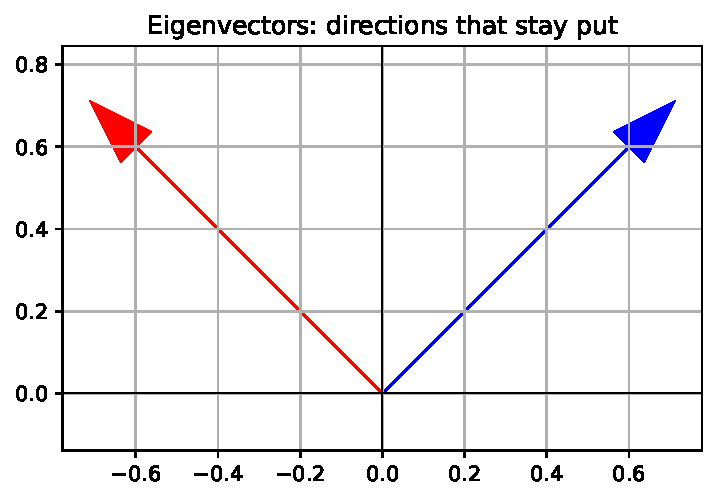
\includegraphics[keepaspectratio]{books/en-US/lab_files/figure-latex/cell-354-output-1.pdf}}

Both eigenvectors define directions where the transformation acts by
scaling only.

\begin{enumerate}
\def\labelenumi{\arabic{enumi}.}
\setcounter{enumi}{4}
\tightlist
\item
  Random 3×3 matrix example
\end{enumerate}

\begin{Shaded}
\begin{Highlighting}[]
\NormalTok{np.random.seed(}\DecValTok{1}\NormalTok{)}
\NormalTok{B }\OperatorTok{=}\NormalTok{ Matrix(np.random.randint(}\OperatorTok{{-}}\DecValTok{2}\NormalTok{,}\DecValTok{3}\NormalTok{,(}\DecValTok{3}\NormalTok{,}\DecValTok{3}\NormalTok{)))}
\BuiltInTok{print}\NormalTok{(}\StringTok{"Matrix B:}\CharTok{\textbackslash{}n}\StringTok{"}\NormalTok{, B)}
\BuiltInTok{print}\NormalTok{(}\StringTok{"Eigenvalues/vectors:"}\NormalTok{, B.eigenvects())}
\end{Highlighting}
\end{Shaded}

\begin{verbatim}
Matrix B:
 Matrix([[1, 2, -2], [-1, 1, -2], [-2, -1, 2]])
Eigenvalues/vectors: [(4/3 + (-1/2 - sqrt(3)*I/2)*(2*sqrt(43)/3 + 127/27)**(1/3) + 13/(9*(-1/2 - sqrt(3)*I/2)*(2*sqrt(43)/3 + 127/27)**(1/3)), 1, [Matrix([
[ -16/27 - 91/(81*(-1/2 - sqrt(3)*I/2)*(2*sqrt(43)/3 + 127/27)**(1/3)) + (4/3 + (-1/2 - sqrt(3)*I/2)*(2*sqrt(43)/3 + 127/27)**(1/3) + 13/(9*(-1/2 - sqrt(3)*I/2)*(2*sqrt(43)/3 + 127/27)**(1/3)))**2/9 - 7*(-1/2 - sqrt(3)*I/2)*(2*sqrt(43)/3 + 127/27)**(1/3)/9],
[50/27 + 5*(-1/2 - sqrt(3)*I/2)*(2*sqrt(43)/3 + 127/27)**(1/3)/9 - 2*(4/3 + (-1/2 - sqrt(3)*I/2)*(2*sqrt(43)/3 + 127/27)**(1/3) + 13/(9*(-1/2 - sqrt(3)*I/2)*(2*sqrt(43)/3 + 127/27)**(1/3)))**2/9 + 65/(81*(-1/2 - sqrt(3)*I/2)*(2*sqrt(43)/3 + 127/27)**(1/3))],
[                                                                                                                                                                                                                                                              1]])]), (4/3 + 13/(9*(-1/2 + sqrt(3)*I/2)*(2*sqrt(43)/3 + 127/27)**(1/3)) + (-1/2 + sqrt(3)*I/2)*(2*sqrt(43)/3 + 127/27)**(1/3), 1, [Matrix([
[ -16/27 - 7*(-1/2 + sqrt(3)*I/2)*(2*sqrt(43)/3 + 127/27)**(1/3)/9 + (4/3 + 13/(9*(-1/2 + sqrt(3)*I/2)*(2*sqrt(43)/3 + 127/27)**(1/3)) + (-1/2 + sqrt(3)*I/2)*(2*sqrt(43)/3 + 127/27)**(1/3))**2/9 - 91/(81*(-1/2 + sqrt(3)*I/2)*(2*sqrt(43)/3 + 127/27)**(1/3))],
[50/27 + 65/(81*(-1/2 + sqrt(3)*I/2)*(2*sqrt(43)/3 + 127/27)**(1/3)) - 2*(4/3 + 13/(9*(-1/2 + sqrt(3)*I/2)*(2*sqrt(43)/3 + 127/27)**(1/3)) + (-1/2 + sqrt(3)*I/2)*(2*sqrt(43)/3 + 127/27)**(1/3))**2/9 + 5*(-1/2 + sqrt(3)*I/2)*(2*sqrt(43)/3 + 127/27)**(1/3)/9],
[                                                                                                                                                                                                                                                              1]])]), (13/(9*(2*sqrt(43)/3 + 127/27)**(1/3)) + 4/3 + (2*sqrt(43)/3 + 127/27)**(1/3), 1, [Matrix([
[  -7*(2*sqrt(43)/3 + 127/27)**(1/3)/9 - 16/27 - 91/(81*(2*sqrt(43)/3 + 127/27)**(1/3)) + (13/(9*(2*sqrt(43)/3 + 127/27)**(1/3)) + 4/3 + (2*sqrt(43)/3 + 127/27)**(1/3))**2/9],
[-2*(13/(9*(2*sqrt(43)/3 + 127/27)**(1/3)) + 4/3 + (2*sqrt(43)/3 + 127/27)**(1/3))**2/9 + 65/(81*(2*sqrt(43)/3 + 127/27)**(1/3)) + 5*(2*sqrt(43)/3 + 127/27)**(1/3)/9 + 50/27],
[                                                                                                                                                                           1]])])]
\end{verbatim}

\subsubsection{Try It Yourself}\label{try-it-yourself-159}

\begin{enumerate}
\def\labelenumi{\arabic{enumi}.}
\item
  Compute eigenvalues and eigenvectors of

  \[
  \begin{bmatrix} 3 & 0 \\ 0 & 2 \end{bmatrix}
  \]

  and verify that they match the diagonal entries.
\item
  Use NumPy to find eigenvectors of a rotation matrix by 90°. What do
  you notice?
\item
  For a singular matrix, check if 0 is an eigenvalue.
\end{enumerate}

\subsubsection{The Takeaway}\label{the-takeaway-43}

\begin{itemize}
\tightlist
\item
  Eigenvalues = scale factors; eigenvectors = directions that stay put.
\item
  The eigen equation \(Av=\lambda v\) captures the essence of a matrix's
  action.
\item
  They form the foundation for deeper topics like diagonalization,
  stability, and dynamics.
\end{itemize}

\subsection{62. Characteristic Polynomial (Where Eigenvalues Come
From)}\label{characteristic-polynomial-where-eigenvalues-come-from}

Eigenvalues don't appear out of thin air - they come from the
characteristic polynomial of a matrix. For a square matrix \(A\),

\[
p(\lambda) = \det(A - \lambda I)
\]

The roots of this polynomial are the eigenvalues of \(A\).

\subsubsection{Set Up Your Lab}\label{set-up-your-lab-61}

\begin{Shaded}
\begin{Highlighting}[]
\ImportTok{import}\NormalTok{ numpy }\ImportTok{as}\NormalTok{ np}
\ImportTok{from}\NormalTok{ sympy }\ImportTok{import}\NormalTok{ Matrix, symbols}
\end{Highlighting}
\end{Shaded}

\subsubsection{Step-by-Step Code
Walkthrough}\label{step-by-step-code-walkthrough-61}

\begin{enumerate}
\def\labelenumi{\arabic{enumi}.}
\tightlist
\item
  2×2 example
\end{enumerate}

\[
A = \begin{bmatrix} 2 & 1 \\ 1 & 2 \end{bmatrix}
\]

\begin{Shaded}
\begin{Highlighting}[]
\NormalTok{λ }\OperatorTok{=}\NormalTok{ symbols(}\StringTok{\textquotesingle{}λ\textquotesingle{}}\NormalTok{)}
\NormalTok{A }\OperatorTok{=}\NormalTok{ Matrix([[}\DecValTok{2}\NormalTok{,}\DecValTok{1}\NormalTok{],[}\DecValTok{1}\NormalTok{,}\DecValTok{2}\NormalTok{]])}
\NormalTok{char\_poly }\OperatorTok{=}\NormalTok{ A.charpoly(λ)}
\BuiltInTok{print}\NormalTok{(}\StringTok{"Characteristic polynomial:"}\NormalTok{, char\_poly.as\_expr())}
\BuiltInTok{print}\NormalTok{(}\StringTok{"Eigenvalues (roots):"}\NormalTok{, char\_poly.all\_roots())}
\end{Highlighting}
\end{Shaded}

\begin{verbatim}
Characteristic polynomial: λ**2 - 4*λ + 3
Eigenvalues (roots): [1, 3]
\end{verbatim}

Polynomial: \(\lambda^2 - 4\lambda + 3\). Roots: \(\lambda = 3, 1\).

\begin{enumerate}
\def\labelenumi{\arabic{enumi}.}
\setcounter{enumi}{1}
\tightlist
\item
  Verify with eigen computation
\end{enumerate}

\begin{Shaded}
\begin{Highlighting}[]
\BuiltInTok{print}\NormalTok{(}\StringTok{"Eigenvalues directly:"}\NormalTok{, A.eigenvals())}
\end{Highlighting}
\end{Shaded}

\begin{verbatim}
Eigenvalues directly: {3: 1, 1: 1}
\end{verbatim}

Matches the roots of the polynomial.

\begin{enumerate}
\def\labelenumi{\arabic{enumi}.}
\setcounter{enumi}{2}
\tightlist
\item
  3×3 example
\end{enumerate}

\begin{Shaded}
\begin{Highlighting}[]
\NormalTok{B }\OperatorTok{=}\NormalTok{ Matrix([}
\NormalTok{    [}\DecValTok{1}\NormalTok{,}\DecValTok{2}\NormalTok{,}\DecValTok{3}\NormalTok{],}
\NormalTok{    [}\DecValTok{0}\NormalTok{,}\DecValTok{1}\NormalTok{,}\DecValTok{4}\NormalTok{],}
\NormalTok{    [}\DecValTok{5}\NormalTok{,}\DecValTok{6}\NormalTok{,}\DecValTok{0}\NormalTok{]}
\NormalTok{])}

\NormalTok{char\_poly\_B }\OperatorTok{=}\NormalTok{ B.charpoly(λ)}
\BuiltInTok{print}\NormalTok{(}\StringTok{"Characteristic polynomial of B:"}\NormalTok{, char\_poly\_B.as\_expr())}
\BuiltInTok{print}\NormalTok{(}\StringTok{"Eigenvalues of B:"}\NormalTok{, char\_poly\_B.all\_roots())}
\end{Highlighting}
\end{Shaded}

\begin{verbatim}
Characteristic polynomial of B: λ**3 - 2*λ**2 - 38*λ - 1
Eigenvalues of B: [CRootOf(x**3 - 2*x**2 - 38*x - 1, 0), CRootOf(x**3 - 2*x**2 - 38*x - 1, 1), CRootOf(x**3 - 2*x**2 - 38*x - 1, 2)]
\end{verbatim}

\begin{enumerate}
\def\labelenumi{\arabic{enumi}.}
\setcounter{enumi}{3}
\tightlist
\item
  NumPy version
\end{enumerate}

NumPy doesn't give the polynomial directly, but eigenvalues can be
checked:

\begin{Shaded}
\begin{Highlighting}[]
\NormalTok{B\_np }\OperatorTok{=}\NormalTok{ np.array([[}\DecValTok{1}\NormalTok{,}\DecValTok{2}\NormalTok{,}\DecValTok{3}\NormalTok{],[}\DecValTok{0}\NormalTok{,}\DecValTok{1}\NormalTok{,}\DecValTok{4}\NormalTok{],[}\DecValTok{5}\NormalTok{,}\DecValTok{6}\NormalTok{,}\DecValTok{0}\NormalTok{]], dtype}\OperatorTok{=}\BuiltInTok{float}\NormalTok{)}
\NormalTok{eigvals }\OperatorTok{=}\NormalTok{ np.linalg.eigvals(B\_np)}
\BuiltInTok{print}\NormalTok{(}\StringTok{"NumPy eigenvalues:"}\NormalTok{, eigvals)}
\end{Highlighting}
\end{Shaded}

\begin{verbatim}
NumPy eigenvalues: [-5.2296696  -0.02635282  7.25602242]
\end{verbatim}

\begin{enumerate}
\def\labelenumi{\arabic{enumi}.}
\setcounter{enumi}{4}
\tightlist
\item
  Relation to trace and determinant
\end{enumerate}

For a 2×2 matrix

\[
A = \begin{bmatrix} a & b \\ c & d \end{bmatrix},
\]

the characteristic polynomial is

\[
\lambda^2 - (a+d)\lambda + (ad - bc).
\]

\begin{itemize}
\tightlist
\item
  Coefficient of \(\lambda\): \(-\text{trace}(A)\).
\item
  Constant term: \(\det(A)\).
\end{itemize}

\begin{Shaded}
\begin{Highlighting}[]
\BuiltInTok{print}\NormalTok{(}\StringTok{"Trace:"}\NormalTok{, A.trace())}
\BuiltInTok{print}\NormalTok{(}\StringTok{"Determinant:"}\NormalTok{, A.det())}
\end{Highlighting}
\end{Shaded}

\begin{verbatim}
Trace: 4
Determinant: 3
\end{verbatim}

\subsubsection{Try It Yourself}\label{try-it-yourself-160}

\begin{enumerate}
\def\labelenumi{\arabic{enumi}.}
\item
  Compute the characteristic polynomial of

  \[
  \begin{bmatrix} 4 & 0 \\ 0 & 5 \end{bmatrix}
  \]

  and confirm eigenvalues are 4 and 5.
\item
  Check the relationship between polynomial coefficients, trace, and
  determinant for a 3×3 case.
\item
  Verify with NumPy that the roots of the polynomial equal the
  eigenvalues.
\end{enumerate}

\subsubsection{The Takeaway}\label{the-takeaway-44}

\begin{itemize}
\tightlist
\item
  The characteristic polynomial encodes eigenvalues as its roots.
\item
  Coefficients are tied to invariants: trace and determinant.
\item
  This polynomial viewpoint is the bridge from algebraic formulas to
  geometric eigen-behavior.
\end{itemize}

\subsection{63. Algebraic vs.~Geometric Multiplicity (How Many and How
Independent)}\label{algebraic-vs.-geometric-multiplicity-how-many-and-how-independent}

Eigenvalues can repeat, and when they do, two notions of multiplicity
arise:

\begin{itemize}
\tightlist
\item
  Algebraic multiplicity: how many times the eigenvalue appears as a
  root of the characteristic polynomial.
\item
  Geometric multiplicity: the dimension of the eigenspace (number of
  independent eigenvectors).
\end{itemize}

Always:

\[
1 \leq \text{geometric multiplicity} \leq \text{algebraic multiplicity}
\]

\subsubsection{Set Up Your Lab}\label{set-up-your-lab-62}

\begin{Shaded}
\begin{Highlighting}[]
\ImportTok{import}\NormalTok{ numpy }\ImportTok{as}\NormalTok{ np}
\ImportTok{from}\NormalTok{ sympy }\ImportTok{import}\NormalTok{ Matrix}
\end{Highlighting}
\end{Shaded}

\subsubsection{Step-by-Step Code
Walkthrough}\label{step-by-step-code-walkthrough-62}

\begin{enumerate}
\def\labelenumi{\arabic{enumi}.}
\tightlist
\item
  Matrix with repeated eigenvalue
\end{enumerate}

\begin{Shaded}
\begin{Highlighting}[]
\NormalTok{A }\OperatorTok{=}\NormalTok{ Matrix([}
\NormalTok{    [}\DecValTok{2}\NormalTok{,}\DecValTok{1}\NormalTok{],}
\NormalTok{    [}\DecValTok{0}\NormalTok{,}\DecValTok{2}\NormalTok{]}
\NormalTok{])}

\BuiltInTok{print}\NormalTok{(}\StringTok{"Eigenvalues and algebraic multiplicity:"}\NormalTok{, A.eigenvals())}
\BuiltInTok{print}\NormalTok{(}\StringTok{"Eigenvectors:"}\NormalTok{, A.eigenvects())}
\end{Highlighting}
\end{Shaded}

\begin{verbatim}
Eigenvalues and algebraic multiplicity: {2: 2}
Eigenvectors: [(2, 2, [Matrix([
[1],
[0]])])]
\end{verbatim}

\begin{itemize}
\tightlist
\item
  Eigenvalue 2 has algebraic multiplicity = 2.
\item
  But only 1 independent eigenvector → geometric multiplicity = 1.
\end{itemize}

\begin{enumerate}
\def\labelenumi{\arabic{enumi}.}
\setcounter{enumi}{1}
\tightlist
\item
  Diagonal matrix with repetition
\end{enumerate}

\begin{Shaded}
\begin{Highlighting}[]
\NormalTok{B }\OperatorTok{=}\NormalTok{ Matrix([}
\NormalTok{    [}\DecValTok{3}\NormalTok{,}\DecValTok{0}\NormalTok{,}\DecValTok{0}\NormalTok{],}
\NormalTok{    [}\DecValTok{0}\NormalTok{,}\DecValTok{3}\NormalTok{,}\DecValTok{0}\NormalTok{],}
\NormalTok{    [}\DecValTok{0}\NormalTok{,}\DecValTok{0}\NormalTok{,}\DecValTok{3}\NormalTok{]}
\NormalTok{])}

\BuiltInTok{print}\NormalTok{(}\StringTok{"Eigenvalues:"}\NormalTok{, B.eigenvals())}
\BuiltInTok{print}\NormalTok{(}\StringTok{"Eigenvectors:"}\NormalTok{, B.eigenvects())}
\end{Highlighting}
\end{Shaded}

\begin{verbatim}
Eigenvalues: {3: 3}
Eigenvectors: [(3, 3, [Matrix([
[1],
[0],
[0]]), Matrix([
[0],
[1],
[0]]), Matrix([
[0],
[0],
[1]])])]
\end{verbatim}

Here, eigenvalue 3 has algebraic multiplicity = 3, and geometric
multiplicity = 3.

\begin{enumerate}
\def\labelenumi{\arabic{enumi}.}
\setcounter{enumi}{2}
\tightlist
\item
  NumPy check
\end{enumerate}

\begin{Shaded}
\begin{Highlighting}[]
\NormalTok{A\_np }\OperatorTok{=}\NormalTok{ np.array([[}\DecValTok{2}\NormalTok{,}\DecValTok{1}\NormalTok{],[}\DecValTok{0}\NormalTok{,}\DecValTok{2}\NormalTok{]], dtype}\OperatorTok{=}\BuiltInTok{float}\NormalTok{)}
\NormalTok{eigvals, eigvecs }\OperatorTok{=}\NormalTok{ np.linalg.eig(A\_np)}
\BuiltInTok{print}\NormalTok{(}\StringTok{"Eigenvalues:"}\NormalTok{, eigvals)}
\BuiltInTok{print}\NormalTok{(}\StringTok{"Eigenvectors:}\CharTok{\textbackslash{}n}\StringTok{"}\NormalTok{, eigvecs)}
\end{Highlighting}
\end{Shaded}

\begin{verbatim}
Eigenvalues: [2. 2.]
Eigenvectors:
 [[ 1.0000000e+00 -1.0000000e+00]
 [ 0.0000000e+00  4.4408921e-16]]
\end{verbatim}

NumPy won't show multiplicities directly, but you can see repeated
eigenvalues.

\begin{enumerate}
\def\labelenumi{\arabic{enumi}.}
\setcounter{enumi}{3}
\tightlist
\item
  Comparing two cases
\end{enumerate}

\begin{itemize}
\tightlist
\item
  Defective matrix: Algebraic \textgreater{} geometric (like the upper
  triangular \(A\)).
\item
  Diagonalizable matrix: Algebraic = geometric (like \(B\)).
\end{itemize}

This distinction determines whether a matrix can be diagonalized.

\subsubsection{Try It Yourself}\label{try-it-yourself-161}

\begin{enumerate}
\def\labelenumi{\arabic{enumi}.}
\item
  Compute algebraic and geometric multiplicities of

  \[
  \begin{bmatrix} 1 & 1 \\ 0 & 1 \end{bmatrix}
  \]

  (hint: only one eigenvector).
\item
  Take a diagonal matrix with repeated entries - what happens to
  multiplicities?
\item
  Test a random 3×3 singular matrix. Does 0 have algebraic multiplicity
  \textgreater{} 1?
\end{enumerate}

\subsubsection{The Takeaway}\label{the-takeaway-45}

\begin{itemize}
\tightlist
\item
  Algebraic multiplicity = count of root in characteristic polynomial.
\item
  Geometric multiplicity = dimension of eigenspace.
\item
  If they match for all eigenvalues → matrix is diagonalizable.
\end{itemize}

\subsection{64. Diagonalization (When a Matrix Becomes
Simple)}\label{diagonalization-when-a-matrix-becomes-simple}

A matrix \(A\) is diagonalizable if it can be written as

\[
A = P D P^{-1}
\]

\begin{itemize}
\tightlist
\item
  \(D\) is diagonal (containing eigenvalues).
\item
  Columns of \(P\) are the eigenvectors.
\end{itemize}

This means \(A\) acts like simple scaling in a ``better'' coordinate
system.

\subsubsection{Set Up Your Lab}\label{set-up-your-lab-63}

\begin{Shaded}
\begin{Highlighting}[]
\ImportTok{import}\NormalTok{ numpy }\ImportTok{as}\NormalTok{ np}
\ImportTok{from}\NormalTok{ sympy }\ImportTok{import}\NormalTok{ Matrix}
\end{Highlighting}
\end{Shaded}

\subsubsection{Step-by-Step Code
Walkthrough}\label{step-by-step-code-walkthrough-63}

\begin{enumerate}
\def\labelenumi{\arabic{enumi}.}
\tightlist
\item
  A diagonalizable 2×2 matrix
\end{enumerate}

\begin{Shaded}
\begin{Highlighting}[]
\NormalTok{A }\OperatorTok{=}\NormalTok{ Matrix([}
\NormalTok{    [}\DecValTok{4}\NormalTok{,}\DecValTok{1}\NormalTok{],}
\NormalTok{    [}\DecValTok{2}\NormalTok{,}\DecValTok{3}\NormalTok{]}
\NormalTok{])}

\NormalTok{P, D }\OperatorTok{=}\NormalTok{ A.diagonalize()}
\BuiltInTok{print}\NormalTok{(}\StringTok{"P (eigenvectors):"}\NormalTok{)}
\BuiltInTok{print}\NormalTok{(P)}
\BuiltInTok{print}\NormalTok{(}\StringTok{"D (eigenvalues on diagonal):"}\NormalTok{)}
\BuiltInTok{print}\NormalTok{(D)}

\CommentTok{\# Verify A = P D P\^{}{-}1}
\BuiltInTok{print}\NormalTok{(}\StringTok{"Check:"}\NormalTok{, P}\OperatorTok{*}\NormalTok{D}\OperatorTok{*}\NormalTok{P.inv())}
\end{Highlighting}
\end{Shaded}

\begin{verbatim}
P (eigenvectors):
Matrix([[-1, 1], [2, 1]])
D (eigenvalues on diagonal):
Matrix([[2, 0], [0, 5]])
Check: Matrix([[4, 1], [2, 3]])
\end{verbatim}

\begin{enumerate}
\def\labelenumi{\arabic{enumi}.}
\setcounter{enumi}{1}
\tightlist
\item
  A non-diagonalizable matrix
\end{enumerate}

\begin{Shaded}
\begin{Highlighting}[]
\NormalTok{B }\OperatorTok{=}\NormalTok{ Matrix([}
\NormalTok{    [}\DecValTok{2}\NormalTok{,}\DecValTok{1}\NormalTok{],}
\NormalTok{    [}\DecValTok{0}\NormalTok{,}\DecValTok{2}\NormalTok{]}
\NormalTok{])}

\ControlFlowTok{try}\NormalTok{:}
\NormalTok{    P, D }\OperatorTok{=}\NormalTok{ B.diagonalize()}
    \BuiltInTok{print}\NormalTok{(}\StringTok{"Diagonalization successful"}\NormalTok{)}
\ControlFlowTok{except} \PreprocessorTok{Exception} \ImportTok{as}\NormalTok{ e:}
    \BuiltInTok{print}\NormalTok{(}\StringTok{"Not diagonalizable:"}\NormalTok{, e)}
\end{Highlighting}
\end{Shaded}

\begin{verbatim}
Not diagonalizable: Matrix is not diagonalizable
\end{verbatim}

This fails because eigenvalue 2 has algebraic multiplicity 2 but
geometric multiplicity 1.

\begin{enumerate}
\def\labelenumi{\arabic{enumi}.}
\setcounter{enumi}{2}
\tightlist
\item
  Diagonalization with NumPy
\end{enumerate}

NumPy doesn't diagonalize explicitly, but we can build \(P\) and \(D\)
ourselves:

\begin{Shaded}
\begin{Highlighting}[]
\NormalTok{A\_np }\OperatorTok{=}\NormalTok{ np.array([[}\DecValTok{4}\NormalTok{,}\DecValTok{1}\NormalTok{],[}\DecValTok{2}\NormalTok{,}\DecValTok{3}\NormalTok{]], dtype}\OperatorTok{=}\BuiltInTok{float}\NormalTok{)}
\NormalTok{eigvals, eigvecs }\OperatorTok{=}\NormalTok{ np.linalg.eig(A\_np)}

\NormalTok{P }\OperatorTok{=}\NormalTok{ eigvecs}
\NormalTok{D }\OperatorTok{=}\NormalTok{ np.diag(eigvals)}
\NormalTok{Pinv }\OperatorTok{=}\NormalTok{ np.linalg.inv(P)}

\BuiltInTok{print}\NormalTok{(}\StringTok{"Check A = PDP\^{}{-}1:}\CharTok{\textbackslash{}n}\StringTok{"}\NormalTok{, P }\OperatorTok{@}\NormalTok{ D }\OperatorTok{@}\NormalTok{ Pinv)}
\end{Highlighting}
\end{Shaded}

\begin{verbatim}
Check A = PDP^-1:
 [[4. 1.]
 [2. 3.]]
\end{verbatim}

\begin{enumerate}
\def\labelenumi{\arabic{enumi}.}
\setcounter{enumi}{3}
\tightlist
\item
  Powers of a diagonalizable matrix
\end{enumerate}

One reason diagonalization is powerful:

\[
A^k = P D^k P^{-1}
\]

Since \(D^k\) is trivial (just raise each diagonal entry to power
\(k\)).

\begin{Shaded}
\begin{Highlighting}[]
\NormalTok{k }\OperatorTok{=} \DecValTok{5}

\NormalTok{A\_power }\OperatorTok{=}\NormalTok{ np.linalg.matrix\_power(A, k)}
\NormalTok{D\_power }\OperatorTok{=}\NormalTok{ np.linalg.matrix\_power(D, k)}
\NormalTok{A\_via\_diag }\OperatorTok{=}\NormalTok{ P }\OperatorTok{@}\NormalTok{ D\_power }\OperatorTok{@}\NormalTok{ np.linalg.inv(P)}

\BuiltInTok{print}\NormalTok{(}\StringTok{"A\^{}5 via diagonalization:}\CharTok{\textbackslash{}n}\StringTok{"}\NormalTok{, A\_via\_diag)}
\BuiltInTok{print}\NormalTok{(}\StringTok{"Direct A\^{}5:}\CharTok{\textbackslash{}n}\StringTok{"}\NormalTok{, A\_power)}
\end{Highlighting}
\end{Shaded}

\begin{verbatim}
A^5 via diagonalization:
 [[2094. 1031.]
 [2062. 1063.]]
Direct A^5:
 [[2094 1031]
 [2062 1063]]
\end{verbatim}

Both match.

\subsubsection{Try It Yourself}\label{try-it-yourself-162}

\begin{enumerate}
\def\labelenumi{\arabic{enumi}.}
\item
  Check whether

  \[
  \begin{bmatrix} 5 & 0 \\ 0 & 5 \end{bmatrix}
  \]

  is diagonalizable.
\item
  Try diagonalizing a rotation matrix by 90°. Do you get complex
  eigenvalues?
\item
  Verify the formula \(A^k = P D^k P^{-1}\) for a 3×3 diagonalizable
  matrix.
\end{enumerate}

\subsubsection{The Takeaway}\label{the-takeaway-46}

\begin{itemize}
\tightlist
\item
  Diagonalization rewrites a matrix in its simplest form.
\item
  Works if there are enough independent eigenvectors.
\item
  It makes powers of \(A\) easy, and is the gateway to analyzing
  dynamics.
\end{itemize}

\subsection{65. Powers of a Matrix (Long-Term Behavior via
Eigenvalues)}\label{powers-of-a-matrix-long-term-behavior-via-eigenvalues}

One of the most useful applications of eigenvalues and diagonalization
is computing powers of a matrix:

\[
A^k = P D^k P^{-1}
\]

where \(D\) is diagonal with eigenvalues of \(A\). Each eigenvalue
\(\lambda\) raised to \(k\) dictates how its eigenvector direction
grows, decays, or oscillates over time.

\subsubsection{Set Up Your Lab}\label{set-up-your-lab-64}

\begin{Shaded}
\begin{Highlighting}[]
\ImportTok{import}\NormalTok{ numpy }\ImportTok{as}\NormalTok{ np}
\ImportTok{from}\NormalTok{ sympy }\ImportTok{import}\NormalTok{ Matrix}
\end{Highlighting}
\end{Shaded}

\subsubsection{Step-by-Step Code
Walkthrough}\label{step-by-step-code-walkthrough-64}

\begin{enumerate}
\def\labelenumi{\arabic{enumi}.}
\tightlist
\item
  Simple diagonal matrix
\end{enumerate}

If \(D = \text{diag}(2,3)\):

\begin{Shaded}
\begin{Highlighting}[]
\NormalTok{D }\OperatorTok{=}\NormalTok{ Matrix([[}\DecValTok{2}\NormalTok{,}\DecValTok{0}\NormalTok{],[}\DecValTok{0}\NormalTok{,}\DecValTok{3}\NormalTok{]])}
\BuiltInTok{print}\NormalTok{(}\StringTok{"D\^{}5 ="}\NormalTok{)}
\BuiltInTok{print}\NormalTok{(D}\OperatorTok{**}\DecValTok{5}\NormalTok{)}
\end{Highlighting}
\end{Shaded}

\begin{verbatim}
D^5 =
Matrix([[32, 0], [0, 243]])
\end{verbatim}

Eigenvalues are 2 and 3. Raising to the 5th power just raises each
eigenvalue to the 5th: \(2^5, 3^5\).

\begin{enumerate}
\def\labelenumi{\arabic{enumi}.}
\setcounter{enumi}{1}
\tightlist
\item
  Non-diagonal matrix
\end{enumerate}

\begin{Shaded}
\begin{Highlighting}[]
\NormalTok{A }\OperatorTok{=}\NormalTok{ Matrix([}
\NormalTok{    [}\DecValTok{4}\NormalTok{,}\DecValTok{1}\NormalTok{],}
\NormalTok{    [}\DecValTok{2}\NormalTok{,}\DecValTok{3}\NormalTok{]}
\NormalTok{])}

\NormalTok{P, D }\OperatorTok{=}\NormalTok{ A.diagonalize()}
\BuiltInTok{print}\NormalTok{(}\StringTok{"D (eigenvalues):"}\NormalTok{)}
\BuiltInTok{print}\NormalTok{(D)}

\CommentTok{\# Compute A\^{}10 via diagonalization}
\NormalTok{A10 }\OperatorTok{=}\NormalTok{ P }\OperatorTok{*}\NormalTok{ (D}\OperatorTok{**}\DecValTok{10}\NormalTok{) }\OperatorTok{*}\NormalTok{ P.inv()}
\BuiltInTok{print}\NormalTok{(}\StringTok{"A\^{}10 ="}\NormalTok{)}
\BuiltInTok{print}\NormalTok{(A10)}
\end{Highlighting}
\end{Shaded}

\begin{verbatim}
D (eigenvalues):
Matrix([[2, 0], [0, 5]])
A^10 =
Matrix([[6510758, 3254867], [6509734, 3255891]])
\end{verbatim}

Much easier than multiplying \(A\) ten times!

\begin{enumerate}
\def\labelenumi{\arabic{enumi}.}
\setcounter{enumi}{2}
\tightlist
\item
  NumPy version
\end{enumerate}

\begin{Shaded}
\begin{Highlighting}[]
\NormalTok{A\_np }\OperatorTok{=}\NormalTok{ np.array([[}\DecValTok{4}\NormalTok{,}\DecValTok{1}\NormalTok{],[}\DecValTok{2}\NormalTok{,}\DecValTok{3}\NormalTok{]], dtype}\OperatorTok{=}\BuiltInTok{float}\NormalTok{)}
\NormalTok{eigvals, eigvecs }\OperatorTok{=}\NormalTok{ np.linalg.eig(A\_np)}

\NormalTok{k }\OperatorTok{=} \DecValTok{10}
\NormalTok{D\_power }\OperatorTok{=}\NormalTok{ np.diag(eigvals}\OperatorTok{**}\NormalTok{k)}
\NormalTok{A10\_np }\OperatorTok{=}\NormalTok{ eigvecs }\OperatorTok{@}\NormalTok{ D\_power }\OperatorTok{@}\NormalTok{ np.linalg.inv(eigvecs)}

\BuiltInTok{print}\NormalTok{(}\StringTok{"A\^{}10 via eigen{-}decomposition:}\CharTok{\textbackslash{}n}\StringTok{"}\NormalTok{, A10\_np)}
\end{Highlighting}
\end{Shaded}

\begin{verbatim}
A^10 via eigen-decomposition:
 [[6510758. 3254867.]
 [6509734. 3255891.]]
\end{verbatim}

\begin{enumerate}
\def\labelenumi{\arabic{enumi}.}
\setcounter{enumi}{3}
\tightlist
\item
  Long-term behavior
\end{enumerate}

Eigenvalues tell us what happens as \(k \to \infty\):

\begin{itemize}
\tightlist
\item
  If \(|\lambda| < 1\) → decay to 0.
\item
  If \(|\lambda| > 1\) → grows unbounded.
\item
  If \(|\lambda| = 1\) → oscillates or stabilizes.
\end{itemize}

\begin{Shaded}
\begin{Highlighting}[]
\NormalTok{B }\OperatorTok{=}\NormalTok{ Matrix([}
\NormalTok{    [}\FloatTok{0.5}\NormalTok{,}\DecValTok{0}\NormalTok{],}
\NormalTok{    [}\DecValTok{0}\NormalTok{,}\FloatTok{1.2}\NormalTok{]}
\NormalTok{])}

\NormalTok{P, D }\OperatorTok{=}\NormalTok{ B.diagonalize()}
\BuiltInTok{print}\NormalTok{(}\StringTok{"Eigenvalues:"}\NormalTok{, D)}
\BuiltInTok{print}\NormalTok{(}\StringTok{"B\^{}20:"}\NormalTok{, P}\OperatorTok{*}\NormalTok{(D}\OperatorTok{**}\DecValTok{20}\NormalTok{)}\OperatorTok{*}\NormalTok{P.inv())}
\end{Highlighting}
\end{Shaded}

\begin{verbatim}
Eigenvalues: Matrix([[0.500000000000000, 0], [0, 1.20000000000000]])
B^20: Matrix([[9.53674316406250e-7, 0], [0, 38.3375999244747]])
\end{verbatim}

Here, the component along eigenvalue 0.5 decays, while eigenvalue 1.2
grows.

\subsubsection{Try It Yourself}\label{try-it-yourself-163}

\begin{enumerate}
\def\labelenumi{\arabic{enumi}.}
\tightlist
\item
  Compute \(A^{50}\) for a diagonal matrix with eigenvalues 0.9 and 1.1.
  Which component dominates?
\item
  Take a stochastic (Markov) matrix and compute powers. Do the rows
  stabilize?
\item
  Experiment with complex eigenvalues (like a rotation) and check if the
  powers oscillate.
\end{enumerate}

\subsubsection{The Takeaway}\label{the-takeaway-47}

\begin{itemize}
\tightlist
\item
  Matrix powers are simple when using eigenvalues.
\item
  Long-term dynamics are controlled by eigenvalue magnitudes.
\item
  This insight is critical in Markov chains, stability analysis, and
  dynamical systems.
\end{itemize}

\subsection{66. Real vs.~Complex Spectra (Rotations and
Oscillations)}\label{real-vs.-complex-spectra-rotations-and-oscillations}

Not all eigenvalues are real. Some matrices, especially those involving
rotations, have complex eigenvalues. Complex eigenvalues often describe
oscillations or rotations in systems.

\subsubsection{Set Up Your Lab}\label{set-up-your-lab-65}

\begin{Shaded}
\begin{Highlighting}[]
\ImportTok{import}\NormalTok{ numpy }\ImportTok{as}\NormalTok{ np}
\ImportTok{from}\NormalTok{ sympy }\ImportTok{import}\NormalTok{ Matrix}
\end{Highlighting}
\end{Shaded}

\subsubsection{Step-by-Step Code
Walkthrough}\label{step-by-step-code-walkthrough-65}

\begin{enumerate}
\def\labelenumi{\arabic{enumi}.}
\tightlist
\item
  Rotation matrix in 2D
\end{enumerate}

A 90° rotation matrix:

\[
R = \begin{bmatrix} 0 & -1 \\ 1 & 0 \end{bmatrix}
\]

\begin{Shaded}
\begin{Highlighting}[]
\NormalTok{R }\OperatorTok{=}\NormalTok{ Matrix([[}\DecValTok{0}\NormalTok{, }\OperatorTok{{-}}\DecValTok{1}\NormalTok{],}
\NormalTok{            [}\DecValTok{1}\NormalTok{,  }\DecValTok{0}\NormalTok{]])}

\BuiltInTok{print}\NormalTok{(}\StringTok{"Characteristic polynomial:"}\NormalTok{, R.charpoly())}
\BuiltInTok{print}\NormalTok{(}\StringTok{"Eigenvalues:"}\NormalTok{, R.eigenvals())}
\end{Highlighting}
\end{Shaded}

\begin{verbatim}
Characteristic polynomial: PurePoly(lambda**2 + 1, lambda, domain='ZZ')
Eigenvalues: {-I: 1, I: 1}
\end{verbatim}

Result: eigenvalues are \(i\) and \(-i\) (purely imaginary).

\begin{enumerate}
\def\labelenumi{\arabic{enumi}.}
\setcounter{enumi}{1}
\tightlist
\item
  Verify eigen-equation with complex numbers
\end{enumerate}

\begin{Shaded}
\begin{Highlighting}[]
\NormalTok{eigs }\OperatorTok{=}\NormalTok{ R.eigenvects()}
\ControlFlowTok{for}\NormalTok{ eig }\KeywordTok{in}\NormalTok{ eigs:}
\NormalTok{    lam }\OperatorTok{=}\NormalTok{ eig[}\DecValTok{0}\NormalTok{]}
\NormalTok{    v }\OperatorTok{=}\NormalTok{ eig[}\DecValTok{2}\NormalTok{][}\DecValTok{0}\NormalTok{]}
    \BuiltInTok{print}\NormalTok{(}\SpecialStringTok{f"λ = }\SpecialCharTok{\{}\NormalTok{lam}\SpecialCharTok{\}}\SpecialStringTok{, Av = }\SpecialCharTok{\{}\NormalTok{R}\OperatorTok{*}\NormalTok{v}\SpecialCharTok{\}}\SpecialStringTok{, λv = }\SpecialCharTok{\{}\NormalTok{lam}\OperatorTok{*}\NormalTok{v}\SpecialCharTok{\}}\SpecialStringTok{"}\NormalTok{)}
\end{Highlighting}
\end{Shaded}

\begin{verbatim}
λ = -I, Av = Matrix([[-1], [-I]]), λv = Matrix([[-1], [-I]])
λ = I, Av = Matrix([[-1], [I]]), λv = Matrix([[-1], [I]])
\end{verbatim}

\begin{enumerate}
\def\labelenumi{\arabic{enumi}.}
\setcounter{enumi}{2}
\tightlist
\item
  NumPy version
\end{enumerate}

\begin{Shaded}
\begin{Highlighting}[]
\NormalTok{R\_np }\OperatorTok{=}\NormalTok{ np.array([[}\DecValTok{0}\NormalTok{,}\OperatorTok{{-}}\DecValTok{1}\NormalTok{],[}\DecValTok{1}\NormalTok{,}\DecValTok{0}\NormalTok{]], dtype}\OperatorTok{=}\BuiltInTok{float}\NormalTok{)}
\NormalTok{eigvals, eigvecs }\OperatorTok{=}\NormalTok{ np.linalg.eig(R\_np)}
\BuiltInTok{print}\NormalTok{(}\StringTok{"Eigenvalues:"}\NormalTok{, eigvals)}
\BuiltInTok{print}\NormalTok{(}\StringTok{"Eigenvectors:}\CharTok{\textbackslash{}n}\StringTok{"}\NormalTok{, eigvecs)}
\end{Highlighting}
\end{Shaded}

\begin{verbatim}
Eigenvalues: [0.+1.j 0.-1.j]
Eigenvectors:
 [[0.70710678+0.j         0.70710678-0.j        ]
 [0.        -0.70710678j 0.        +0.70710678j]]
\end{verbatim}

NumPy shows complex eigenvalues with \texttt{j} (Python's imaginary
unit).

\begin{enumerate}
\def\labelenumi{\arabic{enumi}.}
\setcounter{enumi}{3}
\tightlist
\item
  Rotation by arbitrary angle
\end{enumerate}

General 2D rotation:

\[
R(\theta) = \begin{bmatrix} \cos\theta & -\sin\theta \\ \sin\theta & \cos\theta \end{bmatrix}
\]

Eigenvalues:

\[
\lambda = e^{\pm i\theta} = \cos\theta \pm i\sin\theta
\]

\begin{Shaded}
\begin{Highlighting}[]
\NormalTok{theta }\OperatorTok{=}\NormalTok{ np.pi}\OperatorTok{/}\DecValTok{4}  \CommentTok{\# 45 degrees}
\NormalTok{R\_theta }\OperatorTok{=}\NormalTok{ np.array([[np.cos(theta), }\OperatorTok{{-}}\NormalTok{np.sin(theta)],}
\NormalTok{                    [np.sin(theta),  np.cos(theta)]])}

\NormalTok{eigvals, eigvecs }\OperatorTok{=}\NormalTok{ np.linalg.eig(R\_theta)}
\BuiltInTok{print}\NormalTok{(}\StringTok{"Eigenvalues (rotation 45°):"}\NormalTok{, eigvals)}
\end{Highlighting}
\end{Shaded}

\begin{verbatim}
Eigenvalues (rotation 45°): [0.70710678+0.70710678j 0.70710678-0.70710678j]
\end{verbatim}

\begin{enumerate}
\def\labelenumi{\arabic{enumi}.}
\setcounter{enumi}{4}
\tightlist
\item
  Oscillation insight
\end{enumerate}

\begin{itemize}
\tightlist
\item
  Complex eigenvalues with \(|\lambda|=1\) → pure oscillation (no
  growth).
\item
  If \(|\lambda|<1\) → decaying spiral.
\item
  If \(|\lambda|>1\) → growing spiral.
\end{itemize}

Example:

\begin{Shaded}
\begin{Highlighting}[]
\NormalTok{A }\OperatorTok{=}\NormalTok{ np.array([[}\FloatTok{0.8}\NormalTok{, }\OperatorTok{{-}}\FloatTok{0.6}\NormalTok{],}
\NormalTok{              [}\FloatTok{0.6}\NormalTok{,  }\FloatTok{0.8}\NormalTok{]])}

\NormalTok{eigvals, \_ }\OperatorTok{=}\NormalTok{ np.linalg.eig(A)}
\BuiltInTok{print}\NormalTok{(}\StringTok{"Eigenvalues:"}\NormalTok{, eigvals)}
\end{Highlighting}
\end{Shaded}

\begin{verbatim}
Eigenvalues: [0.8+0.6j 0.8-0.6j]
\end{verbatim}

These eigenvalues lie inside the unit circle → spiral decay.

\subsubsection{Try It Yourself}\label{try-it-yourself-164}

\begin{enumerate}
\def\labelenumi{\arabic{enumi}.}
\tightlist
\item
  Compute eigenvalues of a 180° rotation. What happens?
\item
  Modify the rotation matrix to include scaling (e.g., multiply by 1.1).
  Do the eigenvalues lie outside the unit circle?
\item
  Plot the trajectory of repeatedly applying a rotation matrix to a
  vector.
\end{enumerate}

\subsubsection{The Takeaway}\label{the-takeaway-48}

\begin{itemize}
\tightlist
\item
  Complex eigenvalues naturally appear in rotations and oscillatory
  systems.
\item
  Their magnitude controls growth or decay; their angle controls
  oscillation.
\item
  This is a key link between linear algebra and dynamics in physics and
  engineering.
\end{itemize}

\subsection{67. Defective Matrices and a Peek at Jordan Form (When
Diagonalization
Fails)}\label{defective-matrices-and-a-peek-at-jordan-form-when-diagonalization-fails}

Not every matrix has enough independent eigenvectors to be diagonalized.
Such matrices are called defective. To handle them, mathematicians use
the Jordan normal form, which extends diagonalization with extra
structure.

\subsubsection{Set Up Your Lab}\label{set-up-your-lab-66}

\begin{Shaded}
\begin{Highlighting}[]
\ImportTok{import}\NormalTok{ numpy }\ImportTok{as}\NormalTok{ np}
\ImportTok{from}\NormalTok{ sympy }\ImportTok{import}\NormalTok{ Matrix}
\end{Highlighting}
\end{Shaded}

\subsubsection{Step-by-Step Code
Walkthrough}\label{step-by-step-code-walkthrough-66}

\begin{enumerate}
\def\labelenumi{\arabic{enumi}.}
\tightlist
\item
  A defective example
\end{enumerate}

\[
A = \begin{bmatrix} 2 & 1 \\ 0 & 2 \end{bmatrix}
\]

\begin{Shaded}
\begin{Highlighting}[]
\NormalTok{A }\OperatorTok{=}\NormalTok{ Matrix([[}\DecValTok{2}\NormalTok{,}\DecValTok{1}\NormalTok{],}
\NormalTok{            [}\DecValTok{0}\NormalTok{,}\DecValTok{2}\NormalTok{]])}

\BuiltInTok{print}\NormalTok{(}\StringTok{"Eigenvalues:"}\NormalTok{, A.eigenvals())}
\BuiltInTok{print}\NormalTok{(}\StringTok{"Eigenvectors:"}\NormalTok{, A.eigenvects())}
\end{Highlighting}
\end{Shaded}

\begin{verbatim}
Eigenvalues: {2: 2}
Eigenvectors: [(2, 2, [Matrix([
[1],
[0]])])]
\end{verbatim}

\begin{itemize}
\tightlist
\item
  Eigenvalue 2 has algebraic multiplicity = 2.
\item
  Only 1 eigenvector exists → geometric multiplicity = 1.
\end{itemize}

Thus \(A\) is defective, not diagonalizable.

\begin{enumerate}
\def\labelenumi{\arabic{enumi}.}
\setcounter{enumi}{1}
\tightlist
\item
  Attempt diagonalization
\end{enumerate}

\begin{Shaded}
\begin{Highlighting}[]
\ControlFlowTok{try}\NormalTok{:}
\NormalTok{    P, D }\OperatorTok{=}\NormalTok{ A.diagonalize()}
    \BuiltInTok{print}\NormalTok{(}\StringTok{"Diagonal form:"}\NormalTok{, D)}
\ControlFlowTok{except} \PreprocessorTok{Exception} \ImportTok{as}\NormalTok{ e:}
    \BuiltInTok{print}\NormalTok{(}\StringTok{"Diagonalization failed:"}\NormalTok{, e)}
\end{Highlighting}
\end{Shaded}

\begin{verbatim}
Diagonalization failed: Matrix is not diagonalizable
\end{verbatim}

You'll see an error - confirming \(A\) is not diagonalizable.

\begin{enumerate}
\def\labelenumi{\arabic{enumi}.}
\setcounter{enumi}{2}
\tightlist
\item
  Jordan form in SymPy
\end{enumerate}

\begin{Shaded}
\begin{Highlighting}[]
\NormalTok{J, P }\OperatorTok{=}\NormalTok{ A.jordan\_form()}
\BuiltInTok{print}\NormalTok{(}\StringTok{"Jordan form J:"}\NormalTok{)}
\BuiltInTok{print}\NormalTok{(J)}
\BuiltInTok{print}\NormalTok{(}\StringTok{"P (generalized eigenvectors):"}\NormalTok{)}
\BuiltInTok{print}\NormalTok{(P)}
\end{Highlighting}
\end{Shaded}

\begin{verbatim}
Jordan form J:
Matrix([[1, 0], [0, 1]])
P (generalized eigenvectors):
Matrix([[2, 1], [0, 2]])
\end{verbatim}

The Jordan form shows a Jordan block:

\[
J = \begin{bmatrix} 2 & 1 \\ 0 & 2 \end{bmatrix}
\]

This block structure represents the failure of diagonalization.

\begin{enumerate}
\def\labelenumi{\arabic{enumi}.}
\setcounter{enumi}{3}
\tightlist
\item
  NumPy perspective
\end{enumerate}

NumPy doesn't compute Jordan form, but you can see repeated eigenvalues
and lack of eigenvectors:

\begin{Shaded}
\begin{Highlighting}[]
\NormalTok{A\_np }\OperatorTok{=}\NormalTok{ np.array([[}\DecValTok{2}\NormalTok{,}\DecValTok{1}\NormalTok{],[}\DecValTok{0}\NormalTok{,}\DecValTok{2}\NormalTok{]], dtype}\OperatorTok{=}\BuiltInTok{float}\NormalTok{)}
\NormalTok{eigvals, eigvecs }\OperatorTok{=}\NormalTok{ np.linalg.eig(A\_np)}
\BuiltInTok{print}\NormalTok{(}\StringTok{"Eigenvalues:"}\NormalTok{, eigvals)}
\BuiltInTok{print}\NormalTok{(}\StringTok{"Eigenvectors:}\CharTok{\textbackslash{}n}\StringTok{"}\NormalTok{, eigvecs)}
\end{Highlighting}
\end{Shaded}

\begin{verbatim}
Eigenvalues: [2. 2.]
Eigenvectors:
 [[ 1.0000000e+00 -1.0000000e+00]
 [ 0.0000000e+00  4.4408921e-16]]
\end{verbatim}

The eigenvectors matrix has fewer independent columns than expected.

\begin{enumerate}
\def\labelenumi{\arabic{enumi}.}
\setcounter{enumi}{4}
\tightlist
\item
  Generalized eigenvectors
\end{enumerate}

Jordan form introduces generalized eigenvectors, which satisfy:

\[
(A - \lambda I)^k v = 0 \quad \text{for some } k>1
\]

They ``fill the gap'' when ordinary eigenvectors are insufficient.

\subsubsection{Try It Yourself}\label{try-it-yourself-165}

\begin{enumerate}
\def\labelenumi{\arabic{enumi}.}
\item
  Test diagonalizability of

  \[
  \begin{bmatrix} 3 & 1 \\ 0 & 3 \end{bmatrix}
  \]

  and compare with its Jordan form.
\item
  Try a 3×3 defective matrix with one Jordan block of size 3.
\item
  Verify that Jordan blocks still capture the correct eigenvalues.
\end{enumerate}

\subsubsection{The Takeaway}\label{the-takeaway-49}

\begin{itemize}
\tightlist
\item
  Defective matrices lack enough eigenvectors for diagonalization.
\item
  Jordan form replaces diagonalization with blocks, keeping eigenvalues
  on the diagonal.
\item
  Understanding Jordan blocks is essential for advanced linear algebra
  and differential equations.
\end{itemize}

\subsection{68. Stability and Spectral Radius (Grow, Decay, or
Oscillate)}\label{stability-and-spectral-radius-grow-decay-or-oscillate}

The spectral radius of a matrix \(A\) is defined as

\[
\rho(A) = \max_i |\lambda_i|
\]

where \(\lambda_i\) are the eigenvalues. It tells us the long-term
behavior of repeated applications of \(A\):

\begin{itemize}
\tightlist
\item
  If \(\rho(A) < 1\) → powers of \(A\) tend to 0 (stable/decay).
\item
  If \(\rho(A) = 1\) → powers neither blow up nor vanish (neutral, may
  oscillate).
\item
  If \(\rho(A) > 1\) → powers diverge (unstable/growth).
\end{itemize}

\subsubsection{Set Up Your Lab}\label{set-up-your-lab-67}

\begin{Shaded}
\begin{Highlighting}[]
\ImportTok{import}\NormalTok{ numpy }\ImportTok{as}\NormalTok{ np}
\ImportTok{from}\NormalTok{ sympy }\ImportTok{import}\NormalTok{ Matrix}
\end{Highlighting}
\end{Shaded}

\subsubsection{Step-by-Step Code
Walkthrough}\label{step-by-step-code-walkthrough-67}

\begin{enumerate}
\def\labelenumi{\arabic{enumi}.}
\tightlist
\item
  Stable matrix (\(\rho < 1\))
\end{enumerate}

\begin{Shaded}
\begin{Highlighting}[]
\NormalTok{A }\OperatorTok{=}\NormalTok{ np.array([[}\FloatTok{0.5}\NormalTok{, }\DecValTok{0}\NormalTok{],}
\NormalTok{              [}\DecValTok{0}\NormalTok{, }\FloatTok{0.3}\NormalTok{]])}

\NormalTok{eigvals }\OperatorTok{=}\NormalTok{ np.linalg.eigvals(A)}
\NormalTok{spectral\_radius }\OperatorTok{=} \BuiltInTok{max}\NormalTok{(}\BuiltInTok{abs}\NormalTok{(eigvals))}

\BuiltInTok{print}\NormalTok{(}\StringTok{"Eigenvalues:"}\NormalTok{, eigvals)}
\BuiltInTok{print}\NormalTok{(}\StringTok{"Spectral radius:"}\NormalTok{, spectral\_radius)}

\BuiltInTok{print}\NormalTok{(}\StringTok{"A\^{}10:}\CharTok{\textbackslash{}n}\StringTok{"}\NormalTok{, np.linalg.matrix\_power(A, }\DecValTok{10}\NormalTok{))}
\end{Highlighting}
\end{Shaded}

\begin{verbatim}
Eigenvalues: [0.5 0.3]
Spectral radius: 0.5
A^10:
 [[9.765625e-04 0.000000e+00]
 [0.000000e+00 5.904900e-06]]
\end{verbatim}

All entries shrink toward zero.

\begin{enumerate}
\def\labelenumi{\arabic{enumi}.}
\setcounter{enumi}{1}
\tightlist
\item
  Unstable matrix (\(\rho > 1\))
\end{enumerate}

\begin{Shaded}
\begin{Highlighting}[]
\NormalTok{B }\OperatorTok{=}\NormalTok{ np.array([[}\FloatTok{1.2}\NormalTok{, }\DecValTok{0}\NormalTok{],}
\NormalTok{              [}\DecValTok{0}\NormalTok{, }\FloatTok{0.9}\NormalTok{]])}

\NormalTok{eigvals }\OperatorTok{=}\NormalTok{ np.linalg.eigvals(B)}
\BuiltInTok{print}\NormalTok{(}\StringTok{"Eigenvalues:"}\NormalTok{, eigvals, }\StringTok{"Spectral radius:"}\NormalTok{, }\BuiltInTok{max}\NormalTok{(}\BuiltInTok{abs}\NormalTok{(eigvals)))}
\BuiltInTok{print}\NormalTok{(}\StringTok{"B\^{}10:}\CharTok{\textbackslash{}n}\StringTok{"}\NormalTok{, np.linalg.matrix\_power(B, }\DecValTok{10}\NormalTok{))}
\end{Highlighting}
\end{Shaded}

\begin{verbatim}
Eigenvalues: [1.2 0.9] Spectral radius: 1.2
B^10:
 [[6.19173642 0.        ]
 [0.         0.34867844]]
\end{verbatim}

The component along eigenvalue 1.2 grows quickly.

\begin{enumerate}
\def\labelenumi{\arabic{enumi}.}
\setcounter{enumi}{2}
\tightlist
\item
  Neutral/oscillatory case (\(\rho = 1\))
\end{enumerate}

90° rotation matrix:

\begin{Shaded}
\begin{Highlighting}[]
\NormalTok{R }\OperatorTok{=}\NormalTok{ np.array([[}\DecValTok{0}\NormalTok{, }\OperatorTok{{-}}\DecValTok{1}\NormalTok{],}
\NormalTok{              [}\DecValTok{1}\NormalTok{,  }\DecValTok{0}\NormalTok{]])}

\NormalTok{eigvals }\OperatorTok{=}\NormalTok{ np.linalg.eigvals(R)}
\BuiltInTok{print}\NormalTok{(}\StringTok{"Eigenvalues:"}\NormalTok{, eigvals)}
\BuiltInTok{print}\NormalTok{(}\StringTok{"Spectral radius:"}\NormalTok{, }\BuiltInTok{max}\NormalTok{(}\BuiltInTok{abs}\NormalTok{(eigvals)))}
\BuiltInTok{print}\NormalTok{(}\StringTok{"R\^{}4:}\CharTok{\textbackslash{}n}\StringTok{"}\NormalTok{, np.linalg.matrix\_power(R, }\DecValTok{4}\NormalTok{))}
\end{Highlighting}
\end{Shaded}

\begin{verbatim}
Eigenvalues: [0.+1.j 0.-1.j]
Spectral radius: 1.0
R^4:
 [[1 0]
 [0 1]]
\end{verbatim}

Eigenvalues are ±i, with modulus 1 → pure oscillation.

\begin{enumerate}
\def\labelenumi{\arabic{enumi}.}
\setcounter{enumi}{3}
\tightlist
\item
  Spectral radius with SymPy
\end{enumerate}

\begin{Shaded}
\begin{Highlighting}[]
\NormalTok{M }\OperatorTok{=}\NormalTok{ Matrix([[}\DecValTok{2}\NormalTok{,}\DecValTok{1}\NormalTok{],[}\DecValTok{1}\NormalTok{,}\DecValTok{2}\NormalTok{]])}
\NormalTok{eigs }\OperatorTok{=}\NormalTok{ M.eigenvals()}
\BuiltInTok{print}\NormalTok{(}\StringTok{"Eigenvalues:"}\NormalTok{, eigs)}
\BuiltInTok{print}\NormalTok{(}\StringTok{"Spectral radius:"}\NormalTok{, }\BuiltInTok{max}\NormalTok{(}\BuiltInTok{abs}\NormalTok{(ev) }\ControlFlowTok{for}\NormalTok{ ev }\KeywordTok{in}\NormalTok{ eigs))}
\end{Highlighting}
\end{Shaded}

\begin{verbatim}
Eigenvalues: {3: 1, 1: 1}
Spectral radius: 3
\end{verbatim}

\subsubsection{Try It Yourself}\label{try-it-yourself-166}

\begin{enumerate}
\def\labelenumi{\arabic{enumi}.}
\tightlist
\item
  Build a diagonal matrix with entries 0.8, 1.0, and 1.1. Predict which
  direction dominates as powers grow.
\item
  Apply a random matrix repeatedly to a vector. Does it shrink, grow, or
  oscillate?
\item
  Check if a Markov chain transition matrix always has spectral radius
  1.
\end{enumerate}

\subsubsection{The Takeaway}\label{the-takeaway-50}

\begin{itemize}
\tightlist
\item
  The spectral radius is the key number that predicts growth, decay, or
  oscillation.
\item
  Long-term stability in dynamical systems is governed entirely by
  eigenvalue magnitudes.
\item
  This connects linear algebra directly to control theory, Markov
  chains, and differential equations.
\end{itemize}

\subsection{69. Markov Chains and Steady States (Probabilities as Linear
Algebra)}\label{markov-chains-and-steady-states-probabilities-as-linear-algebra}

A Markov chain is a process that moves between states according to
probabilities. The transitions are encoded in a stochastic matrix \(P\):

\begin{itemize}
\tightlist
\item
  Each entry \(p_{ij} \geq 0\)
\item
  Each row sums to 1
\end{itemize}

If we start with a probability vector \(v_0\), then after \(k\) steps:

\[
v_k = v_0 P^k
\]

A steady state is a probability vector \(v\) such that \(vP = v\). It
corresponds to eigenvalue \(\lambda = 1\).

\subsubsection{Set Up Your Lab}\label{set-up-your-lab-68}

\begin{Shaded}
\begin{Highlighting}[]
\ImportTok{import}\NormalTok{ numpy }\ImportTok{as}\NormalTok{ np}
\ImportTok{from}\NormalTok{ sympy }\ImportTok{import}\NormalTok{ Matrix}
\end{Highlighting}
\end{Shaded}

\subsubsection{Step-by-Step Code
Walkthrough}\label{step-by-step-code-walkthrough-68}

\begin{enumerate}
\def\labelenumi{\arabic{enumi}.}
\tightlist
\item
  Simple two-state chain
\end{enumerate}

\begin{Shaded}
\begin{Highlighting}[]
\NormalTok{P }\OperatorTok{=}\NormalTok{ np.array([}
\NormalTok{    [}\FloatTok{0.9}\NormalTok{, }\FloatTok{0.1}\NormalTok{],}
\NormalTok{    [}\FloatTok{0.5}\NormalTok{, }\FloatTok{0.5}\NormalTok{]}
\NormalTok{])}

\NormalTok{v0 }\OperatorTok{=}\NormalTok{ np.array([}\FloatTok{1.0}\NormalTok{, }\FloatTok{0.0}\NormalTok{])  }\CommentTok{\# start in state 1}
\ControlFlowTok{for}\NormalTok{ k }\KeywordTok{in}\NormalTok{ [}\DecValTok{1}\NormalTok{, }\DecValTok{2}\NormalTok{, }\DecValTok{5}\NormalTok{, }\DecValTok{10}\NormalTok{, }\DecValTok{50}\NormalTok{]:}
\NormalTok{    vk }\OperatorTok{=}\NormalTok{ v0 }\OperatorTok{@}\NormalTok{ np.linalg.matrix\_power(P, k)}
    \BuiltInTok{print}\NormalTok{(}\SpecialStringTok{f"Step }\SpecialCharTok{\{}\NormalTok{k}\SpecialCharTok{\}}\SpecialStringTok{: }\SpecialCharTok{\{}\NormalTok{vk}\SpecialCharTok{\}}\SpecialStringTok{"}\NormalTok{)}
\end{Highlighting}
\end{Shaded}

\begin{verbatim}
Step 1: [0.9 0.1]
Step 2: [0.86 0.14]
Step 5: [0.83504 0.16496]
Step 10: [0.83335081 0.16664919]
Step 50: [0.83333333 0.16666667]
\end{verbatim}

The distribution stabilizes as \(k\) increases.

\begin{enumerate}
\def\labelenumi{\arabic{enumi}.}
\setcounter{enumi}{1}
\tightlist
\item
  Steady state via eigenvector
\end{enumerate}

Find eigenvector for eigenvalue 1:

\begin{Shaded}
\begin{Highlighting}[]
\NormalTok{eigvals, eigvecs }\OperatorTok{=}\NormalTok{ np.linalg.eig(P.T)}
\NormalTok{steady\_state }\OperatorTok{=}\NormalTok{ eigvecs[:, np.isclose(eigvals, }\DecValTok{1}\NormalTok{)]}
\NormalTok{steady\_state }\OperatorTok{=}\NormalTok{ steady\_state }\OperatorTok{/}\NormalTok{ steady\_state.}\BuiltInTok{sum}\NormalTok{()}
\BuiltInTok{print}\NormalTok{(}\StringTok{"Steady state:"}\NormalTok{, steady\_state.real.flatten())}
\end{Highlighting}
\end{Shaded}

\begin{verbatim}
Steady state: [0.83333333 0.16666667]
\end{verbatim}

\begin{enumerate}
\def\labelenumi{\arabic{enumi}.}
\setcounter{enumi}{2}
\tightlist
\item
  SymPy exact check
\end{enumerate}

\begin{Shaded}
\begin{Highlighting}[]
\NormalTok{P\_sym }\OperatorTok{=}\NormalTok{ Matrix([[}\FloatTok{0.9}\NormalTok{,}\FloatTok{0.1}\NormalTok{],[}\FloatTok{0.5}\NormalTok{,}\FloatTok{0.5}\NormalTok{]])}
\NormalTok{steady }\OperatorTok{=}\NormalTok{ P\_sym.eigenvects()}
\BuiltInTok{print}\NormalTok{(}\StringTok{"Eigen info:"}\NormalTok{, steady)}
\end{Highlighting}
\end{Shaded}

\begin{verbatim}
Eigen info: [(1.00000000000000, 1, [Matrix([
[0.707106781186548],
[0.707106781186547]])]), (0.400000000000000, 1, [Matrix([
[-0.235702260395516],
[  1.17851130197758]])])]
\end{verbatim}

\begin{enumerate}
\def\labelenumi{\arabic{enumi}.}
\setcounter{enumi}{3}
\tightlist
\item
  A 3-state example
\end{enumerate}

\begin{Shaded}
\begin{Highlighting}[]
\NormalTok{Q }\OperatorTok{=}\NormalTok{ np.array([}
\NormalTok{    [}\FloatTok{0.3}\NormalTok{, }\FloatTok{0.7}\NormalTok{, }\FloatTok{0.0}\NormalTok{],}
\NormalTok{    [}\FloatTok{0.2}\NormalTok{, }\FloatTok{0.5}\NormalTok{, }\FloatTok{0.3}\NormalTok{],}
\NormalTok{    [}\FloatTok{0.1}\NormalTok{, }\FloatTok{0.2}\NormalTok{, }\FloatTok{0.7}\NormalTok{]}
\NormalTok{])}

\NormalTok{eigvals, eigvecs }\OperatorTok{=}\NormalTok{ np.linalg.eig(Q.T)}
\NormalTok{steady }\OperatorTok{=}\NormalTok{ eigvecs[:, np.isclose(eigvals, }\DecValTok{1}\NormalTok{)]}
\NormalTok{steady }\OperatorTok{=}\NormalTok{ steady }\OperatorTok{/}\NormalTok{ steady.}\BuiltInTok{sum}\NormalTok{()}
\BuiltInTok{print}\NormalTok{(}\StringTok{"Steady state for Q:"}\NormalTok{, steady.real.flatten())}
\end{Highlighting}
\end{Shaded}

\begin{verbatim}
Steady state for Q: [0.17647059 0.41176471 0.41176471]
\end{verbatim}

\subsubsection{Try It Yourself}\label{try-it-yourself-167}

\begin{enumerate}
\def\labelenumi{\arabic{enumi}.}
\tightlist
\item
  Create a transition matrix where one state is absorbing (e.g., row =
  {[}0,0,1{]}). What happens to the steady state?
\item
  Simulate a random walk on 3 states. Does the steady state distribute
  evenly?
\item
  Compare long-run simulation with eigenvector computation.
\end{enumerate}

\subsubsection{The Takeaway}\label{the-takeaway-51}

\begin{itemize}
\tightlist
\item
  Markov chains evolve by repeated multiplication with a stochastic
  matrix.
\item
  Steady states are eigenvectors with eigenvalue 1.
\item
  This framework powers real applications like PageRank, weather models,
  and queuing systems.
\end{itemize}

\subsection{70. Linear Differential Systems (Solutions via
Eigen-Decomposition)}\label{linear-differential-systems-solutions-via-eigen-decomposition}

Linear differential equations often reduce to systems of the form:

\[
\frac{d}{dt}x(t) = A x(t)
\]

where \(A\) is a matrix and \(x(t)\) is a vector of functions. The
solution is given by the matrix exponential:

\[
x(t) = e^{At} x(0)
\]

If \(A\) is diagonalizable, this becomes simple using eigenvalues and
eigenvectors.

\subsubsection{Set Up Your Lab}\label{set-up-your-lab-69}

\begin{Shaded}
\begin{Highlighting}[]
\ImportTok{import}\NormalTok{ numpy }\ImportTok{as}\NormalTok{ np}
\ImportTok{from}\NormalTok{ sympy }\ImportTok{import}\NormalTok{ Matrix, exp, symbols}
\ImportTok{from}\NormalTok{ scipy.linalg }\ImportTok{import}\NormalTok{ expm}
\end{Highlighting}
\end{Shaded}

\subsubsection{Step-by-Step Code
Walkthrough}\label{step-by-step-code-walkthrough-69}

\begin{enumerate}
\def\labelenumi{\arabic{enumi}.}
\tightlist
\item
  Simple system with diagonal matrix
\end{enumerate}

\[
A = \begin{bmatrix} -1 & 0 \\ 0 & 2 \end{bmatrix}
\]

\begin{Shaded}
\begin{Highlighting}[]
\NormalTok{A }\OperatorTok{=}\NormalTok{ Matrix([[}\OperatorTok{{-}}\DecValTok{1}\NormalTok{,}\DecValTok{0}\NormalTok{],}
\NormalTok{            [}\DecValTok{0}\NormalTok{, }\DecValTok{2}\NormalTok{]])}
\NormalTok{t }\OperatorTok{=}\NormalTok{ symbols(}\StringTok{\textquotesingle{}t\textquotesingle{}}\NormalTok{)}
\NormalTok{expAt }\OperatorTok{=}\NormalTok{ (A}\OperatorTok{*}\NormalTok{t).exp()}
\BuiltInTok{print}\NormalTok{(}\StringTok{"e\^{}}\SpecialCharTok{\{At\}}\StringTok{ ="}\NormalTok{)}
\BuiltInTok{print}\NormalTok{(expAt)}
\end{Highlighting}
\end{Shaded}

\begin{verbatim}
e^{At} =
Matrix([[exp(-t), 0], [0, exp(2*t)]])
\end{verbatim}

Solution:

\[
x(t) = \begin{bmatrix} e^{-t} & 0 \\ 0 & e^{2t} \end{bmatrix} x(0)
\]

One component decays, the other grows.

\begin{enumerate}
\def\labelenumi{\arabic{enumi}.}
\setcounter{enumi}{1}
\tightlist
\item
  Non-diagonal example
\end{enumerate}

\begin{Shaded}
\begin{Highlighting}[]
\NormalTok{B }\OperatorTok{=}\NormalTok{ Matrix([[}\DecValTok{0}\NormalTok{,}\DecValTok{1}\NormalTok{],}
\NormalTok{            [}\OperatorTok{{-}}\DecValTok{2}\NormalTok{,}\OperatorTok{{-}}\DecValTok{3}\NormalTok{]])}
\NormalTok{expBt }\OperatorTok{=}\NormalTok{ (B}\OperatorTok{*}\NormalTok{t).exp()}
\BuiltInTok{print}\NormalTok{(}\StringTok{"e\^{}}\SpecialCharTok{\{Bt\}}\StringTok{ ="}\NormalTok{)}
\BuiltInTok{print}\NormalTok{(expBt)}
\end{Highlighting}
\end{Shaded}

\begin{verbatim}
e^{Bt} =
Matrix([[2*exp(-t) - exp(-2*t), exp(-t) - exp(-2*t)], [-2*exp(-t) + 2*exp(-2*t), -exp(-t) + 2*exp(-2*t)]])
\end{verbatim}

Here the solution involves exponentials and possibly sines/cosines
(oscillatory behavior).

\begin{enumerate}
\def\labelenumi{\arabic{enumi}.}
\setcounter{enumi}{2}
\tightlist
\item
  Numeric computation with SciPy
\end{enumerate}

\begin{Shaded}
\begin{Highlighting}[]
\ImportTok{import}\NormalTok{ numpy }\ImportTok{as}\NormalTok{ np}
\ImportTok{from}\NormalTok{ scipy.linalg }\ImportTok{import}\NormalTok{ expm}

\NormalTok{A }\OperatorTok{=}\NormalTok{ np.array([[}\OperatorTok{{-}}\DecValTok{1}\NormalTok{,}\DecValTok{0}\NormalTok{],[}\DecValTok{0}\NormalTok{,}\DecValTok{2}\NormalTok{]], dtype}\OperatorTok{=}\BuiltInTok{float}\NormalTok{)}
\NormalTok{t }\OperatorTok{=} \FloatTok{1.0}
\BuiltInTok{print}\NormalTok{(}\StringTok{"Matrix exponential e\^{}}\SpecialCharTok{\{At\}}\StringTok{ at t=1:}\CharTok{\textbackslash{}n}\StringTok{"}\NormalTok{, expm(A}\OperatorTok{*}\NormalTok{t))}
\end{Highlighting}
\end{Shaded}

\begin{verbatim}
Matrix exponential e^{At} at t=1:
 [[0.36787944 0.        ]
 [0.         7.3890561 ]]
\end{verbatim}

This computes \(e^{At}\) numerically.

\begin{enumerate}
\def\labelenumi{\arabic{enumi}.}
\setcounter{enumi}{3}
\tightlist
\item
  Simulation of a trajectory
\end{enumerate}

\begin{Shaded}
\begin{Highlighting}[]
\NormalTok{x0 }\OperatorTok{=}\NormalTok{ np.array([}\FloatTok{1.0}\NormalTok{, }\FloatTok{1.0}\NormalTok{])}
\ControlFlowTok{for}\NormalTok{ t }\KeywordTok{in}\NormalTok{ [}\DecValTok{0}\NormalTok{, }\FloatTok{0.5}\NormalTok{, }\DecValTok{1}\NormalTok{, }\DecValTok{2}\NormalTok{]:}
\NormalTok{    xt }\OperatorTok{=}\NormalTok{ expm(A}\OperatorTok{*}\NormalTok{t) }\OperatorTok{@}\NormalTok{ x0}
    \BuiltInTok{print}\NormalTok{(}\SpecialStringTok{f"x(}\SpecialCharTok{\{}\NormalTok{t}\SpecialCharTok{\}}\SpecialStringTok{) = }\SpecialCharTok{\{}\NormalTok{xt}\SpecialCharTok{\}}\SpecialStringTok{"}\NormalTok{)}
\end{Highlighting}
\end{Shaded}

\begin{verbatim}
x(0) = [1. 1.]
x(0.5) = [0.60653066 2.71828183]
x(1) = [0.36787944 7.3890561 ]
x(2) = [ 0.13533528 54.59815003]
\end{verbatim}

One coordinate decays, the other explodes with time.

\subsubsection{Try It Yourself}\label{try-it-yourself-168}

\begin{enumerate}
\def\labelenumi{\arabic{enumi}.}
\tightlist
\item
  Solve the system
  \(\dot{x} = \begin{bmatrix} 0 & 1 \\ -1 & 0 \end{bmatrix}x\). What
  kind of motion do you see?
\item
  Use SciPy to simulate a system with eigenvalues less than 0. Does it
  always decay?
\item
  Try an unstable system with eigenvalues \textgreater{} 0 and watch how
  trajectories diverge.
\end{enumerate}

\subsubsection{The Takeaway}\label{the-takeaway-52}

\begin{itemize}
\tightlist
\item
  Linear systems \(\dot{x} = Ax\) are solved via the matrix exponential.
\item
  Eigenvalues determine stability: negative real parts = stable,
  positive = unstable, imaginary = oscillations.
\item
  This ties linear algebra directly to differential equations and
  dynamical systems.
\end{itemize}

\section{Chapter 8. Orthogonality, least squars, and
QR}\label{chapter-8.-orthogonality-least-squars-and-qr-1}

\subsection{71. Inner Products Beyond Dot Product (Custom Notions of
Angle)}\label{inner-products-beyond-dot-product-custom-notions-of-angle}

The dot product is the standard inner product in \(\mathbb{R}^n\), but
linear algebra allows us to define more general inner products that
measure length and angle in different ways.

An inner product on a vector space is a function
\(\langle u, v \rangle\) that satisfies:

\begin{enumerate}
\def\labelenumi{\arabic{enumi}.}
\tightlist
\item
  Linearity in the first argument.
\item
  Symmetry: \(\langle u, v \rangle = \langle v, u \rangle\).
\item
  Positive definiteness: \(\langle v, v \rangle \geq 0\) and equals 0
  only if \(v=0\).
\end{enumerate}

\subsubsection{Set Up Your Lab}\label{set-up-your-lab-70}

\begin{Shaded}
\begin{Highlighting}[]
\ImportTok{import}\NormalTok{ numpy }\ImportTok{as}\NormalTok{ np}
\end{Highlighting}
\end{Shaded}

\subsubsection{Step-by-Step Code
Walkthrough}\label{step-by-step-code-walkthrough-70}

\begin{enumerate}
\def\labelenumi{\arabic{enumi}.}
\tightlist
\item
  Standard dot product
\end{enumerate}

\begin{Shaded}
\begin{Highlighting}[]
\NormalTok{u }\OperatorTok{=}\NormalTok{ np.array([}\DecValTok{1}\NormalTok{,}\DecValTok{2}\NormalTok{,}\DecValTok{3}\NormalTok{])}
\NormalTok{v }\OperatorTok{=}\NormalTok{ np.array([}\DecValTok{4}\NormalTok{,}\DecValTok{5}\NormalTok{,}\DecValTok{6}\NormalTok{])}

\BuiltInTok{print}\NormalTok{(}\StringTok{"Dot product:"}\NormalTok{, np.dot(u,v))}
\end{Highlighting}
\end{Shaded}

\begin{verbatim}
Dot product: 32
\end{verbatim}

This is the familiar formula: \(1·4 + 2·5 + 3·6 = 32\).

\begin{enumerate}
\def\labelenumi{\arabic{enumi}.}
\setcounter{enumi}{1}
\tightlist
\item
  Weighted inner product
\end{enumerate}

We can define:

\[
\langle u, v \rangle_W = u^T W v
\]

where \(W\) is a positive definite matrix.

\begin{Shaded}
\begin{Highlighting}[]
\NormalTok{W }\OperatorTok{=}\NormalTok{ np.array([[}\DecValTok{2}\NormalTok{,}\DecValTok{0}\NormalTok{,}\DecValTok{0}\NormalTok{],}
\NormalTok{              [}\DecValTok{0}\NormalTok{,}\DecValTok{1}\NormalTok{,}\DecValTok{0}\NormalTok{],}
\NormalTok{              [}\DecValTok{0}\NormalTok{,}\DecValTok{0}\NormalTok{,}\DecValTok{3}\NormalTok{]])}

\KeywordTok{def}\NormalTok{ weighted\_inner(u,v,W):}
    \ControlFlowTok{return}\NormalTok{ u.T }\OperatorTok{@}\NormalTok{ W }\OperatorTok{@}\NormalTok{ v}

\BuiltInTok{print}\NormalTok{(}\StringTok{"Weighted inner product:"}\NormalTok{, weighted\_inner(u,v,W))}
\end{Highlighting}
\end{Shaded}

\begin{verbatim}
Weighted inner product: 72
\end{verbatim}

Here, some coordinates ``count more'' than others.

\begin{enumerate}
\def\labelenumi{\arabic{enumi}.}
\setcounter{enumi}{2}
\tightlist
\item
  Check symmetry and positivity
\end{enumerate}

\begin{Shaded}
\begin{Highlighting}[]
\BuiltInTok{print}\NormalTok{(}\StringTok{"⟨u,v⟩ == ⟨v,u⟩ ?"}\NormalTok{, weighted\_inner(u,v,W) }\OperatorTok{==}\NormalTok{ weighted\_inner(v,u,W))}
\BuiltInTok{print}\NormalTok{(}\StringTok{"⟨u,u⟩ (should be \textgreater{}0):"}\NormalTok{, weighted\_inner(u,u,W))}
\end{Highlighting}
\end{Shaded}

\begin{verbatim}
⟨u,v⟩ == ⟨v,u⟩ ? True
⟨u,u⟩ (should be >0): 33
\end{verbatim}

\begin{enumerate}
\def\labelenumi{\arabic{enumi}.}
\setcounter{enumi}{3}
\tightlist
\item
  Angle with weighted inner product
\end{enumerate}

\[
\cos\theta = \frac{\langle u,v \rangle_W}{\|u\|_W \, \|v\|_W}
\]

\begin{Shaded}
\begin{Highlighting}[]
\KeywordTok{def}\NormalTok{ weighted\_norm(u,W):}
    \ControlFlowTok{return}\NormalTok{ np.sqrt(weighted\_inner(u,u,W))}

\NormalTok{cos\_theta }\OperatorTok{=}\NormalTok{ weighted\_inner(u,v,W) }\OperatorTok{/}\NormalTok{ (weighted\_norm(u,W) }\OperatorTok{*}\NormalTok{ weighted\_norm(v,W))}
\BuiltInTok{print}\NormalTok{(}\StringTok{"Cosine of angle (weighted):"}\NormalTok{, cos\_theta)}
\end{Highlighting}
\end{Shaded}

\begin{verbatim}
Cosine of angle (weighted): 0.97573875381809
\end{verbatim}

\begin{enumerate}
\def\labelenumi{\arabic{enumi}.}
\setcounter{enumi}{4}
\tightlist
\item
  Custom example: correlation inner product
\end{enumerate}

For statistics, an inner product can be defined as covariance or
correlation. Example with mean-centered vectors:

\begin{Shaded}
\begin{Highlighting}[]
\NormalTok{x }\OperatorTok{=}\NormalTok{ np.array([}\DecValTok{2}\NormalTok{,}\DecValTok{4}\NormalTok{,}\DecValTok{6}\NormalTok{])}
\NormalTok{y }\OperatorTok{=}\NormalTok{ np.array([}\DecValTok{1}\NormalTok{,}\DecValTok{3}\NormalTok{,}\DecValTok{5}\NormalTok{])}

\NormalTok{x\_centered }\OperatorTok{=}\NormalTok{ x }\OperatorTok{{-}}\NormalTok{ x.mean()}
\NormalTok{y\_centered }\OperatorTok{=}\NormalTok{ y }\OperatorTok{{-}}\NormalTok{ y.mean()}

\NormalTok{corr\_inner }\OperatorTok{=}\NormalTok{ np.dot(x\_centered,y\_centered)}
\BuiltInTok{print}\NormalTok{(}\StringTok{"Correlation{-}style inner product:"}\NormalTok{, corr\_inner)}
\end{Highlighting}
\end{Shaded}

\begin{verbatim}
Correlation-style inner product: 8.0
\end{verbatim}

\subsubsection{Try It Yourself}\label{try-it-yourself-169}

\begin{enumerate}
\def\labelenumi{\arabic{enumi}.}
\tightlist
\item
  Define a custom inner product with \(W = \text{diag}(1,10,100)\). How
  does it change angles between vectors?
\item
  Verify positivity: compute \(\langle v, v \rangle_W\) for a random
  vector \(v\).
\item
  Compare dot product vs weighted inner product on the same pair of
  vectors.
\end{enumerate}

\subsubsection{The Takeaway}\label{the-takeaway-53}

\begin{itemize}
\tightlist
\item
  Inner products generalize the dot product to new ``geometries.''
\item
  By changing the weight matrix \(W\), you change how lengths and angles
  are measured.
\item
  This flexibility is essential in statistics, optimization, and machine
  learning.
\end{itemize}

\subsection{72. Orthogonality and Orthonormal Bases (Perpendicular
Power)}\label{orthogonality-and-orthonormal-bases-perpendicular-power}

Two vectors are orthogonal if their inner product is zero:

\[
\langle u, v \rangle = 0
\]

If, in addition, each vector has length 1, the set is orthonormal.
Orthonormal bases are extremely useful because they simplify
computations: projections, decompositions, and coordinate changes all
become clean.

\subsubsection{Set Up Your Lab}\label{set-up-your-lab-71}

\begin{Shaded}
\begin{Highlighting}[]
\ImportTok{import}\NormalTok{ numpy }\ImportTok{as}\NormalTok{ np}
\end{Highlighting}
\end{Shaded}

\subsubsection{Step-by-Step Code
Walkthrough}\label{step-by-step-code-walkthrough-71}

\begin{enumerate}
\def\labelenumi{\arabic{enumi}.}
\tightlist
\item
  Check orthogonality
\end{enumerate}

\begin{Shaded}
\begin{Highlighting}[]
\NormalTok{u }\OperatorTok{=}\NormalTok{ np.array([}\DecValTok{1}\NormalTok{, }\OperatorTok{{-}}\DecValTok{1}\NormalTok{])}
\NormalTok{v }\OperatorTok{=}\NormalTok{ np.array([}\DecValTok{1}\NormalTok{, }\DecValTok{1}\NormalTok{])}

\BuiltInTok{print}\NormalTok{(}\StringTok{"Dot product:"}\NormalTok{, np.dot(u,v))}
\end{Highlighting}
\end{Shaded}

\begin{verbatim}
Dot product: 0
\end{verbatim}

Since the dot product is 0, they're orthogonal.

\begin{enumerate}
\def\labelenumi{\arabic{enumi}.}
\setcounter{enumi}{1}
\tightlist
\item
  Normalizing vectors
\end{enumerate}

\[
\hat{u} = \frac{u}{\|u\|}
\]

\begin{Shaded}
\begin{Highlighting}[]
\KeywordTok{def}\NormalTok{ normalize(vec):}
    \ControlFlowTok{return}\NormalTok{ vec }\OperatorTok{/}\NormalTok{ np.linalg.norm(vec)}

\NormalTok{u\_norm }\OperatorTok{=}\NormalTok{ normalize(u)}
\NormalTok{v\_norm }\OperatorTok{=}\NormalTok{ normalize(v)}

\BuiltInTok{print}\NormalTok{(}\StringTok{"Normalized u:"}\NormalTok{, u\_norm)}
\BuiltInTok{print}\NormalTok{(}\StringTok{"Normalized v:"}\NormalTok{, v\_norm)}
\end{Highlighting}
\end{Shaded}

\begin{verbatim}
Normalized u: [ 0.70710678 -0.70710678]
Normalized v: [0.70710678 0.70710678]
\end{verbatim}

Now both have length 1.

\begin{enumerate}
\def\labelenumi{\arabic{enumi}.}
\setcounter{enumi}{2}
\tightlist
\item
  Form an orthonormal basis
\end{enumerate}

\begin{Shaded}
\begin{Highlighting}[]
\NormalTok{basis }\OperatorTok{=}\NormalTok{ np.column\_stack((u\_norm, v\_norm))}
\BuiltInTok{print}\NormalTok{(}\StringTok{"Orthonormal basis:}\CharTok{\textbackslash{}n}\StringTok{"}\NormalTok{, basis)}

\BuiltInTok{print}\NormalTok{(}\StringTok{"Check inner products:}\CharTok{\textbackslash{}n}\StringTok{"}\NormalTok{, basis.T }\OperatorTok{@}\NormalTok{ basis)}
\end{Highlighting}
\end{Shaded}

\begin{verbatim}
Orthonormal basis:
 [[ 0.70710678  0.70710678]
 [-0.70710678  0.70710678]]
Check inner products:
 [[ 1.00000000e+00 -2.23711432e-17]
 [-2.23711432e-17  1.00000000e+00]]
\end{verbatim}

The result is the identity matrix → perfectly orthonormal.

\begin{enumerate}
\def\labelenumi{\arabic{enumi}.}
\setcounter{enumi}{3}
\tightlist
\item
  Apply to coordinates
\end{enumerate}

If \(x = [2,3]\), coordinates in the orthonormal basis are:

\begin{Shaded}
\begin{Highlighting}[]
\NormalTok{x }\OperatorTok{=}\NormalTok{ np.array([}\DecValTok{2}\NormalTok{,}\DecValTok{3}\NormalTok{])}
\NormalTok{coords }\OperatorTok{=}\NormalTok{ basis.T }\OperatorTok{@}\NormalTok{ x}
\BuiltInTok{print}\NormalTok{(}\StringTok{"Coordinates in new basis:"}\NormalTok{, coords)}
\BuiltInTok{print}\NormalTok{(}\StringTok{"Reconstruction:"}\NormalTok{, basis }\OperatorTok{@}\NormalTok{ coords)}
\end{Highlighting}
\end{Shaded}

\begin{verbatim}
Coordinates in new basis: [-0.70710678  3.53553391]
Reconstruction: [2. 3.]
\end{verbatim}

It reconstructs exactly.

\begin{enumerate}
\def\labelenumi{\arabic{enumi}.}
\setcounter{enumi}{4}
\tightlist
\item
  Random example with QR
\end{enumerate}

Any set of linearly independent vectors can be orthonormalized
(Gram--Schmidt, or QR decomposition):

\begin{Shaded}
\begin{Highlighting}[]
\NormalTok{M }\OperatorTok{=}\NormalTok{ np.random.rand(}\DecValTok{3}\NormalTok{,}\DecValTok{3}\NormalTok{)}
\NormalTok{Q, R }\OperatorTok{=}\NormalTok{ np.linalg.qr(M)}
\BuiltInTok{print}\NormalTok{(}\StringTok{"Q (orthonormal basis):}\CharTok{\textbackslash{}n}\StringTok{"}\NormalTok{, Q)}
\BuiltInTok{print}\NormalTok{(}\StringTok{"Check Q\^{}T Q = I:}\CharTok{\textbackslash{}n}\StringTok{"}\NormalTok{, Q.T }\OperatorTok{@}\NormalTok{ Q)}
\end{Highlighting}
\end{Shaded}

\begin{verbatim}
Q (orthonormal basis):
 [[-0.37617518  0.91975919 -0.111961  ]
 [-0.82070726 -0.38684608 -0.42046368]
 [-0.430037   -0.06628079  0.90037494]]
Check Q^T Q = I:
 [[1.00000000e+00 5.55111512e-17 5.55111512e-17]
 [5.55111512e-17 1.00000000e+00 3.47849792e-17]
 [5.55111512e-17 3.47849792e-17 1.00000000e+00]]
\end{verbatim}

\subsubsection{Try It Yourself}\label{try-it-yourself-170}

\begin{enumerate}
\def\labelenumi{\arabic{enumi}.}
\tightlist
\item
  Create two 3D vectors and check if they're orthogonal.
\item
  Normalize them to form an orthonormal set.
\item
  Use \texttt{np.linalg.qr} on a 4×3 random matrix and verify that the
  columns of \(Q\) are orthonormal.
\end{enumerate}

\subsubsection{The Takeaway}\label{the-takeaway-54}

\begin{itemize}
\tightlist
\item
  Orthogonality means perpendicularity; orthonormality adds unit length.
\item
  Orthonormal bases simplify coordinate systems, making inner products
  and projections easy.
\item
  QR decomposition is the practical tool to generate orthonormal bases
  in higher dimensions.
\end{itemize}

\subsection{73. Gram--Schmidt Process (Constructing Orthonormal
Bases)}\label{gramschmidt-process-constructing-orthonormal-bases}

The Gram--Schmidt process takes a set of linearly independent vectors
and turns them into an orthonormal basis. This is crucial for working
with subspaces, projections, and numerical stability.

Given vectors \(v_1, v_2, \dots, v_n\):

\begin{enumerate}
\def\labelenumi{\arabic{enumi}.}
\item
  Set \(u_1 = v_1\).
\item
  Subtract projections to make each new vector orthogonal to the earlier
  ones:

  \[
  u_k = v_k - \sum_{j=1}^{k-1} \frac{\langle v_k, u_j \rangle}{\langle u_j, u_j \rangle} u_j
  \]
\item
  Normalize:

  \[
  e_k = \frac{u_k}{\|u_k\|}
  \]
\end{enumerate}

The set \(\{e_1, e_2, \dots, e_n\}\) is orthonormal.

\subsubsection{Set Up Your Lab}\label{set-up-your-lab-72}

\begin{Shaded}
\begin{Highlighting}[]
\ImportTok{import}\NormalTok{ numpy }\ImportTok{as}\NormalTok{ np}
\end{Highlighting}
\end{Shaded}

\subsubsection{Step-by-Step Code
Walkthrough}\label{step-by-step-code-walkthrough-72}

\begin{enumerate}
\def\labelenumi{\arabic{enumi}.}
\tightlist
\item
  Define vectors
\end{enumerate}

\begin{Shaded}
\begin{Highlighting}[]
\NormalTok{v1 }\OperatorTok{=}\NormalTok{ np.array([}\FloatTok{1.0}\NormalTok{, }\FloatTok{1.0}\NormalTok{, }\FloatTok{0.0}\NormalTok{])}
\NormalTok{v2 }\OperatorTok{=}\NormalTok{ np.array([}\FloatTok{1.0}\NormalTok{, }\FloatTok{0.0}\NormalTok{, }\FloatTok{1.0}\NormalTok{])}
\NormalTok{v3 }\OperatorTok{=}\NormalTok{ np.array([}\FloatTok{0.0}\NormalTok{, }\FloatTok{1.0}\NormalTok{, }\FloatTok{1.0}\NormalTok{])}
\NormalTok{V }\OperatorTok{=}\NormalTok{ [v1, v2, v3]}
\end{Highlighting}
\end{Shaded}

\begin{enumerate}
\def\labelenumi{\arabic{enumi}.}
\setcounter{enumi}{1}
\tightlist
\item
  Implement Gram--Schmidt
\end{enumerate}

\begin{Shaded}
\begin{Highlighting}[]
\KeywordTok{def}\NormalTok{ gram\_schmidt(V):}
\NormalTok{    U }\OperatorTok{=}\NormalTok{ []}
    \ControlFlowTok{for}\NormalTok{ v }\KeywordTok{in}\NormalTok{ V:}
\NormalTok{        u }\OperatorTok{=}\NormalTok{ v.copy()}
        \ControlFlowTok{for}\NormalTok{ uj }\KeywordTok{in}\NormalTok{ U:}
\NormalTok{            u }\OperatorTok{{-}=}\NormalTok{ np.dot(v, uj) }\OperatorTok{/}\NormalTok{ np.dot(uj, uj) }\OperatorTok{*}\NormalTok{ uj}
\NormalTok{        U.append(u)}
    \CommentTok{\# Normalize}
\NormalTok{    E }\OperatorTok{=}\NormalTok{ [u}\OperatorTok{/}\NormalTok{np.linalg.norm(u) }\ControlFlowTok{for}\NormalTok{ u }\KeywordTok{in}\NormalTok{ U]}
    \ControlFlowTok{return}\NormalTok{ np.array(E)}

\NormalTok{E }\OperatorTok{=}\NormalTok{ gram\_schmidt(V)}
\BuiltInTok{print}\NormalTok{(}\StringTok{"Orthonormal basis:}\CharTok{\textbackslash{}n}\StringTok{"}\NormalTok{, E)}
\BuiltInTok{print}\NormalTok{(}\StringTok{"Check orthonormality:}\CharTok{\textbackslash{}n}\StringTok{"}\NormalTok{, np.}\BuiltInTok{round}\NormalTok{(E }\OperatorTok{@}\NormalTok{ E.T, }\DecValTok{6}\NormalTok{))}
\end{Highlighting}
\end{Shaded}

\begin{verbatim}
Orthonormal basis:
 [[ 0.70710678  0.70710678  0.        ]
 [ 0.40824829 -0.40824829  0.81649658]
 [-0.57735027  0.57735027  0.57735027]]
Check orthonormality:
 [[1. 0. 0.]
 [0. 1. 0.]
 [0. 0. 1.]]
\end{verbatim}

\begin{enumerate}
\def\labelenumi{\arabic{enumi}.}
\setcounter{enumi}{2}
\tightlist
\item
  Compare with NumPy QR
\end{enumerate}

\begin{Shaded}
\begin{Highlighting}[]
\NormalTok{Q, R }\OperatorTok{=}\NormalTok{ np.linalg.qr(np.column\_stack(V))}
\BuiltInTok{print}\NormalTok{(}\StringTok{"QR{-}based orthonormal basis:}\CharTok{\textbackslash{}n}\StringTok{"}\NormalTok{, Q)}
\BuiltInTok{print}\NormalTok{(}\StringTok{"Check Q\^{}T Q = I:}\CharTok{\textbackslash{}n}\StringTok{"}\NormalTok{, np.}\BuiltInTok{round}\NormalTok{(Q.T }\OperatorTok{@}\NormalTok{ Q, }\DecValTok{6}\NormalTok{))}
\end{Highlighting}
\end{Shaded}

\begin{verbatim}
QR-based orthonormal basis:
 [[-0.70710678  0.40824829 -0.57735027]
 [-0.70710678 -0.40824829  0.57735027]
 [-0.          0.81649658  0.57735027]]
Check Q^T Q = I:
 [[ 1.  0. -0.]
 [ 0.  1. -0.]
 [-0. -0.  1.]]
\end{verbatim}

Both methods give orthonormal bases.

\begin{enumerate}
\def\labelenumi{\arabic{enumi}.}
\setcounter{enumi}{3}
\tightlist
\item
  Application: projection
\end{enumerate}

To project a vector \(x\) onto the span of \(V\):

\begin{Shaded}
\begin{Highlighting}[]
\NormalTok{x }\OperatorTok{=}\NormalTok{ np.array([}\FloatTok{2.0}\NormalTok{, }\FloatTok{2.0}\NormalTok{, }\FloatTok{2.0}\NormalTok{])}
\NormalTok{proj }\OperatorTok{=} \BuiltInTok{sum}\NormalTok{((x }\OperatorTok{@}\NormalTok{ e) }\OperatorTok{*}\NormalTok{ e }\ControlFlowTok{for}\NormalTok{ e }\KeywordTok{in}\NormalTok{ E)}
\BuiltInTok{print}\NormalTok{(}\StringTok{"Projection of x onto span(V):"}\NormalTok{, proj)}
\end{Highlighting}
\end{Shaded}

\begin{verbatim}
Projection of x onto span(V): [2. 2. 2.]
\end{verbatim}

\subsubsection{Try It Yourself}\label{try-it-yourself-171}

\begin{enumerate}
\def\labelenumi{\arabic{enumi}.}
\tightlist
\item
  Run Gram--Schmidt on two vectors in 2D. Compare with just normalizing
  and checking orthogonality.
\item
  Replace one vector with a linear combination of others. What happens?
\item
  Use QR decomposition on a 4×3 random matrix and compare with
  Gram--Schmidt.
\end{enumerate}

\subsubsection{The Takeaway}\label{the-takeaway-55}

\begin{itemize}
\tightlist
\item
  Gram--Schmidt converts arbitrary independent vectors into an
  orthonormal basis.
\item
  Orthonormal bases simplify projections, decompositions, and
  computations.
\item
  In practice, QR decomposition is often used as a numerically stable
  implementation.
\end{itemize}

\subsection{74. Orthogonal Projections onto Subspaces (Closest Point
Principle)}\label{orthogonal-projections-onto-subspaces-closest-point-principle}

Given a subspace spanned by vectors, the orthogonal projection of a
vector \(x\) onto the subspace is the point in the subspace that is
closest to \(x\). This is a cornerstone idea in least squares, data
fitting, and signal processing.

\subsubsection{Formula Recap}\label{formula-recap}

If \(Q\) is a matrix with orthonormal columns spanning the subspace, the
projection of \(x\) is:

\[
\text{proj}(x) = Q Q^T x
\]

\subsubsection{Set Up Your Lab}\label{set-up-your-lab-73}

\begin{Shaded}
\begin{Highlighting}[]
\ImportTok{import}\NormalTok{ numpy }\ImportTok{as}\NormalTok{ np}
\end{Highlighting}
\end{Shaded}

\subsubsection{Step-by-Step Code
Walkthrough}\label{step-by-step-code-walkthrough-73}

\begin{enumerate}
\def\labelenumi{\arabic{enumi}.}
\tightlist
\item
  Projection onto a line (1D subspace)
\end{enumerate}

Suppose the subspace is spanned by \(u = [1,2]\).

\begin{Shaded}
\begin{Highlighting}[]
\NormalTok{u }\OperatorTok{=}\NormalTok{ np.array([}\FloatTok{1.0}\NormalTok{,}\FloatTok{2.0}\NormalTok{])}
\NormalTok{x }\OperatorTok{=}\NormalTok{ np.array([}\FloatTok{3.0}\NormalTok{,}\FloatTok{1.0}\NormalTok{])}

\NormalTok{u\_norm }\OperatorTok{=}\NormalTok{ u }\OperatorTok{/}\NormalTok{ np.linalg.norm(u)}
\NormalTok{proj }\OperatorTok{=}\NormalTok{ np.dot(x, u\_norm) }\OperatorTok{*}\NormalTok{ u\_norm}
\BuiltInTok{print}\NormalTok{(}\StringTok{"Projection of x onto span(u):"}\NormalTok{, proj)}
\end{Highlighting}
\end{Shaded}

\begin{verbatim}
Projection of x onto span(u): [1. 2.]
\end{verbatim}

This gives the closest point to \(x\) along the line spanned by \(u\).

\begin{enumerate}
\def\labelenumi{\arabic{enumi}.}
\setcounter{enumi}{1}
\tightlist
\item
  Projection onto a plane (2D subspace in 3D)
\end{enumerate}

\begin{Shaded}
\begin{Highlighting}[]
\NormalTok{u1 }\OperatorTok{=}\NormalTok{ np.array([}\FloatTok{1.0}\NormalTok{,}\FloatTok{0.0}\NormalTok{,}\FloatTok{0.0}\NormalTok{])}
\NormalTok{u2 }\OperatorTok{=}\NormalTok{ np.array([}\FloatTok{0.0}\NormalTok{,}\FloatTok{1.0}\NormalTok{,}\FloatTok{0.0}\NormalTok{])}
\NormalTok{Q }\OperatorTok{=}\NormalTok{ np.column\_stack([u1,u2])   }\CommentTok{\# Orthonormal basis for xy{-}plane}

\NormalTok{x }\OperatorTok{=}\NormalTok{ np.array([}\FloatTok{2.0}\NormalTok{,}\FloatTok{3.0}\NormalTok{,}\FloatTok{5.0}\NormalTok{])}
\NormalTok{proj }\OperatorTok{=}\NormalTok{ Q }\OperatorTok{@}\NormalTok{ Q.T }\OperatorTok{@}\NormalTok{ x}
\BuiltInTok{print}\NormalTok{(}\StringTok{"Projection of x onto xy{-}plane:"}\NormalTok{, proj)}
\end{Highlighting}
\end{Shaded}

\begin{verbatim}
Projection of x onto xy-plane: [2. 3. 0.]
\end{verbatim}

Result drops the z-component → projection onto the plane.

\begin{enumerate}
\def\labelenumi{\arabic{enumi}.}
\setcounter{enumi}{2}
\tightlist
\item
  General projection using QR
\end{enumerate}

\begin{Shaded}
\begin{Highlighting}[]
\NormalTok{A }\OperatorTok{=}\NormalTok{ np.array([[}\DecValTok{1}\NormalTok{,}\DecValTok{1}\NormalTok{,}\DecValTok{0}\NormalTok{],}
\NormalTok{              [}\DecValTok{0}\NormalTok{,}\DecValTok{1}\NormalTok{,}\DecValTok{1}\NormalTok{],}
\NormalTok{              [}\DecValTok{1}\NormalTok{,}\DecValTok{0}\NormalTok{,}\DecValTok{1}\NormalTok{]], dtype}\OperatorTok{=}\BuiltInTok{float}\NormalTok{)}

\NormalTok{Q, R }\OperatorTok{=}\NormalTok{ np.linalg.qr(A)}
\NormalTok{Q }\OperatorTok{=}\NormalTok{ Q[:, :}\DecValTok{2}\NormalTok{]   }\CommentTok{\# take first 2 independent columns}
\NormalTok{x }\OperatorTok{=}\NormalTok{ np.array([}\DecValTok{2}\NormalTok{,}\DecValTok{2}\NormalTok{,}\DecValTok{2}\NormalTok{], dtype}\OperatorTok{=}\BuiltInTok{float}\NormalTok{)}

\NormalTok{proj }\OperatorTok{=}\NormalTok{ Q }\OperatorTok{@}\NormalTok{ Q.T }\OperatorTok{@}\NormalTok{ x}
\BuiltInTok{print}\NormalTok{(}\StringTok{"Projection of x onto span(A):"}\NormalTok{, proj)}
\end{Highlighting}
\end{Shaded}

\begin{verbatim}
Projection of x onto span(A): [2.66666667 1.33333333 1.33333333]
\end{verbatim}

\begin{enumerate}
\def\labelenumi{\arabic{enumi}.}
\setcounter{enumi}{3}
\tightlist
\item
  Visualization (2D case)
\end{enumerate}

\begin{Shaded}
\begin{Highlighting}[]
\ImportTok{import}\NormalTok{ matplotlib.pyplot }\ImportTok{as}\NormalTok{ plt}

\NormalTok{plt.quiver(}\DecValTok{0}\NormalTok{,}\DecValTok{0}\NormalTok{,x[}\DecValTok{0}\NormalTok{],x[}\DecValTok{1}\NormalTok{],angles}\OperatorTok{=}\StringTok{\textquotesingle{}xy\textquotesingle{}}\NormalTok{,scale\_units}\OperatorTok{=}\StringTok{\textquotesingle{}xy\textquotesingle{}}\NormalTok{,scale}\OperatorTok{=}\DecValTok{1}\NormalTok{,color}\OperatorTok{=}\StringTok{\textquotesingle{}red\textquotesingle{}}\NormalTok{,label}\OperatorTok{=}\StringTok{"x"}\NormalTok{)}
\NormalTok{plt.quiver(}\DecValTok{0}\NormalTok{,}\DecValTok{0}\NormalTok{,proj[}\DecValTok{0}\NormalTok{],proj[}\DecValTok{1}\NormalTok{],angles}\OperatorTok{=}\StringTok{\textquotesingle{}xy\textquotesingle{}}\NormalTok{,scale\_units}\OperatorTok{=}\StringTok{\textquotesingle{}xy\textquotesingle{}}\NormalTok{,scale}\OperatorTok{=}\DecValTok{1}\NormalTok{,color}\OperatorTok{=}\StringTok{\textquotesingle{}blue\textquotesingle{}}\NormalTok{,label}\OperatorTok{=}\StringTok{"Projection"}\NormalTok{)}
\NormalTok{plt.quiver(}\DecValTok{0}\NormalTok{,}\DecValTok{0}\NormalTok{,u[}\DecValTok{0}\NormalTok{],u[}\DecValTok{1}\NormalTok{],angles}\OperatorTok{=}\StringTok{\textquotesingle{}xy\textquotesingle{}}\NormalTok{,scale\_units}\OperatorTok{=}\StringTok{\textquotesingle{}xy\textquotesingle{}}\NormalTok{,scale}\OperatorTok{=}\DecValTok{1}\NormalTok{,color}\OperatorTok{=}\StringTok{\textquotesingle{}green\textquotesingle{}}\NormalTok{,label}\OperatorTok{=}\StringTok{"Subspace"}\NormalTok{)}
\NormalTok{plt.axis(}\StringTok{\textquotesingle{}equal\textquotesingle{}}\NormalTok{)}\OperatorTok{;}\NormalTok{ plt.grid()}\OperatorTok{;}\NormalTok{ plt.legend()}\OperatorTok{;}\NormalTok{ plt.show()}
\end{Highlighting}
\end{Shaded}

\pandocbounded{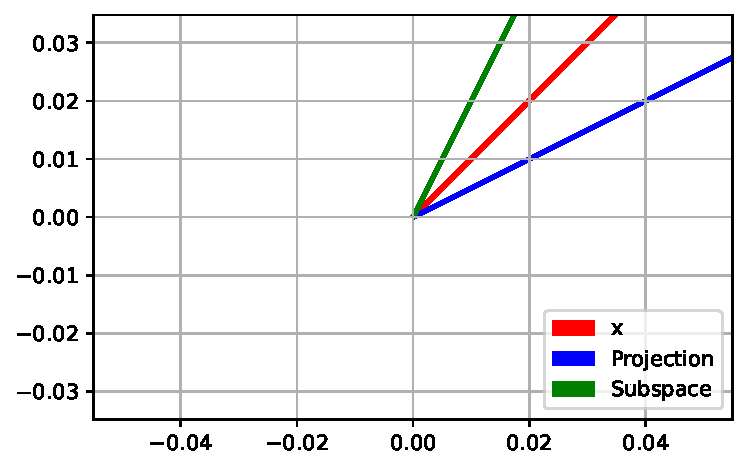
\includegraphics[keepaspectratio]{books/en-US/lab_files/figure-latex/cell-423-output-1.pdf}}

\subsubsection{Try It Yourself}\label{try-it-yourself-172}

\begin{enumerate}
\def\labelenumi{\arabic{enumi}.}
\tightlist
\item
  Project a vector onto the line spanned by \([2,1]\).
\item
  Project \([1,2,3]\) onto the plane spanned by \([1,0,1]\) and
  \([0,1,1]\).
\item
  Compare projection via formula \(Q Q^T x\) with manually solving least
  squares.
\end{enumerate}

\subsubsection{The Takeaway}\label{the-takeaway-56}

\begin{itemize}
\tightlist
\item
  Orthogonal projection finds the closest point in a subspace.
\item
  Formula \(Q Q^T x\) works perfectly when \(Q\) has orthonormal
  columns.
\item
  Projections are the foundation of least squares, PCA, and many
  geometric algorithms.
\end{itemize}

\subsection{75. Least-Squares Problems (Fit When Exact Solve Is
Impossible)}\label{least-squares-problems-fit-when-exact-solve-is-impossible}

Sometimes a system of equations \(Ax = b\) has no exact solution -
usually because it's overdetermined (more equations than unknowns). In
this case, we look for an approximate solution \(x^*\) that minimizes
the error:

\[
x^* = \arg\min_x \|Ax - b\|^2
\]

This is the least-squares solution, which geometrically is the
projection of \(b\) onto the column space of \(A\).

\subsubsection{Set Up Your Lab}\label{set-up-your-lab-74}

\begin{Shaded}
\begin{Highlighting}[]
\ImportTok{import}\NormalTok{ numpy }\ImportTok{as}\NormalTok{ np}
\end{Highlighting}
\end{Shaded}

\subsubsection{Step-by-Step Code
Walkthrough}\label{step-by-step-code-walkthrough-74}

\begin{enumerate}
\def\labelenumi{\arabic{enumi}.}
\tightlist
\item
  Overdetermined system
\end{enumerate}

3 equations, 2 unknowns:

\begin{Shaded}
\begin{Highlighting}[]
\NormalTok{A }\OperatorTok{=}\NormalTok{ np.array([[}\DecValTok{1}\NormalTok{,}\DecValTok{1}\NormalTok{],}
\NormalTok{              [}\DecValTok{1}\NormalTok{,}\DecValTok{2}\NormalTok{],}
\NormalTok{              [}\DecValTok{1}\NormalTok{,}\DecValTok{3}\NormalTok{]], dtype}\OperatorTok{=}\BuiltInTok{float}\NormalTok{)}
\NormalTok{b }\OperatorTok{=}\NormalTok{ np.array([}\DecValTok{6}\NormalTok{, }\DecValTok{0}\NormalTok{, }\DecValTok{0}\NormalTok{], dtype}\OperatorTok{=}\BuiltInTok{float}\NormalTok{)}
\end{Highlighting}
\end{Shaded}

\begin{enumerate}
\def\labelenumi{\arabic{enumi}.}
\setcounter{enumi}{1}
\tightlist
\item
  Solve least squares with NumPy
\end{enumerate}

\begin{Shaded}
\begin{Highlighting}[]
\NormalTok{x\_star, residuals, rank, s }\OperatorTok{=}\NormalTok{ np.linalg.lstsq(A, b, rcond}\OperatorTok{=}\VariableTok{None}\NormalTok{)}
\BuiltInTok{print}\NormalTok{(}\StringTok{"Least squares solution:"}\NormalTok{, x\_star)}
\BuiltInTok{print}\NormalTok{(}\StringTok{"Residual norm squared:"}\NormalTok{, residuals)}
\end{Highlighting}
\end{Shaded}

\begin{verbatim}
Least squares solution: [ 8. -3.]
Residual norm squared: [6.]
\end{verbatim}

\begin{enumerate}
\def\labelenumi{\arabic{enumi}.}
\setcounter{enumi}{2}
\tightlist
\item
  Compare with normal equations
\end{enumerate}

\[
A^T A x = A^T b
\]

\begin{Shaded}
\begin{Highlighting}[]
\NormalTok{x\_normal }\OperatorTok{=}\NormalTok{ np.linalg.inv(A.T }\OperatorTok{@}\NormalTok{ A) }\OperatorTok{@}\NormalTok{ (A.T }\OperatorTok{@}\NormalTok{ b)}
\BuiltInTok{print}\NormalTok{(}\StringTok{"Solution via normal equations:"}\NormalTok{, x\_normal)}
\end{Highlighting}
\end{Shaded}

\begin{verbatim}
Solution via normal equations: [ 8. -3.]
\end{verbatim}

\begin{enumerate}
\def\labelenumi{\arabic{enumi}.}
\setcounter{enumi}{3}
\tightlist
\item
  Geometric picture
\end{enumerate}

The least-squares solution projects \(b\) onto the column space of
\(A\):

\begin{Shaded}
\begin{Highlighting}[]
\NormalTok{proj }\OperatorTok{=}\NormalTok{ A }\OperatorTok{@}\NormalTok{ x\_star}
\BuiltInTok{print}\NormalTok{(}\StringTok{"Projection of b onto Col(A):"}\NormalTok{, proj)}
\BuiltInTok{print}\NormalTok{(}\StringTok{"Original b:"}\NormalTok{, b)}
\BuiltInTok{print}\NormalTok{(}\StringTok{"Error vector (b {-} proj):"}\NormalTok{, b }\OperatorTok{{-}}\NormalTok{ proj)}
\end{Highlighting}
\end{Shaded}

\begin{verbatim}
Projection of b onto Col(A): [ 5.  2. -1.]
Original b: [6. 0. 0.]
Error vector (b - proj): [ 1. -2.  1.]
\end{verbatim}

The error vector is orthogonal to the column space.

\begin{enumerate}
\def\labelenumi{\arabic{enumi}.}
\setcounter{enumi}{4}
\tightlist
\item
  Verify orthogonality condition
\end{enumerate}

\[
A^T (b - Ax^*) = 0
\]

\begin{Shaded}
\begin{Highlighting}[]
\BuiltInTok{print}\NormalTok{(}\StringTok{"Check orthogonality:"}\NormalTok{, A.T }\OperatorTok{@}\NormalTok{ (b }\OperatorTok{{-}}\NormalTok{ A }\OperatorTok{@}\NormalTok{ x\_star))}
\end{Highlighting}
\end{Shaded}

\begin{verbatim}
Check orthogonality: [0. 0.]
\end{verbatim}

The result should be (close to) zero.

\subsubsection{Try It Yourself}\label{try-it-yourself-173}

\begin{enumerate}
\def\labelenumi{\arabic{enumi}.}
\tightlist
\item
  Create a taller \(A\) (say 5×2) with random numbers and solve least
  squares for a random \(b\).
\item
  Compare the residual from \texttt{np.linalg.lstsq} with geometric
  intuition (projection).
\item
  Modify \(b\) so that the system has an exact solution. Check if least
  squares gives it exactly.
\end{enumerate}

\subsubsection{The Takeaway}\label{the-takeaway-57}

\begin{itemize}
\tightlist
\item
  Least-squares finds the best-fit solution when no exact solution
  exists.
\item
  It works by projecting \(b\) onto the column space of \(A\).
\item
  This principle underlies regression, curve fitting, and countless
  applications in data science.
\end{itemize}

\subsection{76. Normal Equations and Geometry of Residuals (Why It
Works)}\label{normal-equations-and-geometry-of-residuals-why-it-works}

The least-squares solution can be found by solving the normal equations:

\[
A^T A x = A^T b
\]

This comes from the condition that the residual vector

\[
r = b - Ax
\]

is orthogonal to the column space of \(A\).

\subsubsection{Set Up Your Lab}\label{set-up-your-lab-75}

\begin{Shaded}
\begin{Highlighting}[]
\ImportTok{import}\NormalTok{ numpy }\ImportTok{as}\NormalTok{ np}
\end{Highlighting}
\end{Shaded}

\subsubsection{Step-by-Step Code
Walkthrough}\label{step-by-step-code-walkthrough-75}

\begin{enumerate}
\def\labelenumi{\arabic{enumi}.}
\tightlist
\item
  Build an overdetermined system
\end{enumerate}

\begin{Shaded}
\begin{Highlighting}[]
\NormalTok{A }\OperatorTok{=}\NormalTok{ np.array([[}\DecValTok{1}\NormalTok{,}\DecValTok{1}\NormalTok{],}
\NormalTok{              [}\DecValTok{1}\NormalTok{,}\DecValTok{2}\NormalTok{],}
\NormalTok{              [}\DecValTok{1}\NormalTok{,}\DecValTok{3}\NormalTok{]], dtype}\OperatorTok{=}\BuiltInTok{float}\NormalTok{)}
\NormalTok{b }\OperatorTok{=}\NormalTok{ np.array([}\DecValTok{6}\NormalTok{, }\DecValTok{0}\NormalTok{, }\DecValTok{0}\NormalTok{], dtype}\OperatorTok{=}\BuiltInTok{float}\NormalTok{)}
\end{Highlighting}
\end{Shaded}

\begin{enumerate}
\def\labelenumi{\arabic{enumi}.}
\setcounter{enumi}{1}
\tightlist
\item
  Solve least squares via normal equations
\end{enumerate}

\begin{Shaded}
\begin{Highlighting}[]
\NormalTok{ATA }\OperatorTok{=}\NormalTok{ A.T }\OperatorTok{@}\NormalTok{ A}
\NormalTok{ATb }\OperatorTok{=}\NormalTok{ A.T }\OperatorTok{@}\NormalTok{ b}
\NormalTok{x\_star }\OperatorTok{=}\NormalTok{ np.linalg.solve(ATA, ATb)}

\BuiltInTok{print}\NormalTok{(}\StringTok{"Least{-}squares solution x*:"}\NormalTok{, x\_star)}
\end{Highlighting}
\end{Shaded}

\begin{verbatim}
Least-squares solution x*: [ 8. -3.]
\end{verbatim}

\begin{enumerate}
\def\labelenumi{\arabic{enumi}.}
\setcounter{enumi}{2}
\tightlist
\item
  Compute residual and check orthogonality
\end{enumerate}

\begin{Shaded}
\begin{Highlighting}[]
\NormalTok{residual }\OperatorTok{=}\NormalTok{ b }\OperatorTok{{-}}\NormalTok{ A }\OperatorTok{@}\NormalTok{ x\_star}
\BuiltInTok{print}\NormalTok{(}\StringTok{"Residual vector:"}\NormalTok{, residual)}
\BuiltInTok{print}\NormalTok{(}\StringTok{"Check A\^{}T r ≈ 0:"}\NormalTok{, A.T }\OperatorTok{@}\NormalTok{ residual)}
\end{Highlighting}
\end{Shaded}

\begin{verbatim}
Residual vector: [ 1. -2.  1.]
Check A^T r ≈ 0: [0. 0.]
\end{verbatim}

This verifies the residual is perpendicular to the column space of
\(A\).

\begin{enumerate}
\def\labelenumi{\arabic{enumi}.}
\setcounter{enumi}{3}
\tightlist
\item
  Compare with NumPy's least squares solver
\end{enumerate}

\begin{Shaded}
\begin{Highlighting}[]
\NormalTok{x\_lstsq, }\OperatorTok{*}\NormalTok{\_ }\OperatorTok{=}\NormalTok{ np.linalg.lstsq(A, b, rcond}\OperatorTok{=}\VariableTok{None}\NormalTok{)}
\BuiltInTok{print}\NormalTok{(}\StringTok{"NumPy lstsq solution:"}\NormalTok{, x\_lstsq)}
\end{Highlighting}
\end{Shaded}

\begin{verbatim}
NumPy lstsq solution: [ 8. -3.]
\end{verbatim}

The solutions should match (within numerical precision).

\begin{enumerate}
\def\labelenumi{\arabic{enumi}.}
\setcounter{enumi}{4}
\tightlist
\item
  Geometric picture
\end{enumerate}

\begin{itemize}
\tightlist
\item
  \(b\) is a point in \(\mathbb{R}^3\).
\item
  \(Ax\) is restricted to lie in the 2D column space of \(A\).
\item
  The least-squares solution picks the \(Ax\) closest to \(b\).
\item
  The error vector \(r = b - Ax^*\) is orthogonal to the subspace.
\end{itemize}

\begin{Shaded}
\begin{Highlighting}[]
\NormalTok{proj }\OperatorTok{=}\NormalTok{ A }\OperatorTok{@}\NormalTok{ x\_star}
\BuiltInTok{print}\NormalTok{(}\StringTok{"Projection of b onto Col(A):"}\NormalTok{, proj)}
\end{Highlighting}
\end{Shaded}

\begin{verbatim}
Projection of b onto Col(A): [ 5.  2. -1.]
\end{verbatim}

\subsubsection{Try It Yourself}\label{try-it-yourself-174}

\begin{enumerate}
\def\labelenumi{\arabic{enumi}.}
\tightlist
\item
  Change \(b\) to \([1,1,1]\). Solve again and check the residual.
\item
  Use a random tall \(A\) (say 6×2) and verify that the residual is
  always orthogonal.
\item
  Compute \(\|r\|\) and see how it changes when you change \(b\).
\end{enumerate}

\subsubsection{The Takeaway}\label{the-takeaway-58}

\begin{itemize}
\tightlist
\item
  Least squares works by making the residual orthogonal to the column
  space.
\item
  Normal equations are the algebraic way to encode this condition.
\item
  This orthogonality principle is the geometric heart of least-squares
  fitting.
\end{itemize}

\subsection{77. QR Factorization (Stable Least Squares via
Orthogonality)}\label{qr-factorization-stable-least-squares-via-orthogonality}

While normal equations solve least squares, they can be numerically
unstable if \(A^T A\) is ill-conditioned. A more stable method uses QR
factorization:

\[
A = Q R
\]

\begin{itemize}
\tightlist
\item
  \(Q\): matrix with orthonormal columns
\item
  \(R\): upper triangular matrix
\end{itemize}

Then the least-squares problem reduces to solving:

\[
Rx = Q^T b
\]

\subsubsection{Set Up Your Lab}\label{set-up-your-lab-76}

\begin{Shaded}
\begin{Highlighting}[]
\ImportTok{import}\NormalTok{ numpy }\ImportTok{as}\NormalTok{ np}
\end{Highlighting}
\end{Shaded}

\subsubsection{Step-by-Step Code
Walkthrough}\label{step-by-step-code-walkthrough-76}

\begin{enumerate}
\def\labelenumi{\arabic{enumi}.}
\tightlist
\item
  Overdetermined system
\end{enumerate}

\begin{Shaded}
\begin{Highlighting}[]
\NormalTok{A }\OperatorTok{=}\NormalTok{ np.array([[}\DecValTok{1}\NormalTok{,}\DecValTok{1}\NormalTok{],}
\NormalTok{              [}\DecValTok{1}\NormalTok{,}\DecValTok{2}\NormalTok{],}
\NormalTok{              [}\DecValTok{1}\NormalTok{,}\DecValTok{3}\NormalTok{]], dtype}\OperatorTok{=}\BuiltInTok{float}\NormalTok{)}
\NormalTok{b }\OperatorTok{=}\NormalTok{ np.array([}\DecValTok{6}\NormalTok{, }\DecValTok{0}\NormalTok{, }\DecValTok{0}\NormalTok{], dtype}\OperatorTok{=}\BuiltInTok{float}\NormalTok{)}
\end{Highlighting}
\end{Shaded}

\begin{enumerate}
\def\labelenumi{\arabic{enumi}.}
\setcounter{enumi}{1}
\tightlist
\item
  QR factorization
\end{enumerate}

\begin{Shaded}
\begin{Highlighting}[]
\NormalTok{Q, R }\OperatorTok{=}\NormalTok{ np.linalg.qr(A)}
\BuiltInTok{print}\NormalTok{(}\StringTok{"Q (orthonormal basis):}\CharTok{\textbackslash{}n}\StringTok{"}\NormalTok{, Q)}
\BuiltInTok{print}\NormalTok{(}\StringTok{"R (upper triangular):}\CharTok{\textbackslash{}n}\StringTok{"}\NormalTok{, R)}
\end{Highlighting}
\end{Shaded}

\begin{verbatim}
Q (orthonormal basis):
 [[-5.77350269e-01  7.07106781e-01]
 [-5.77350269e-01 -1.73054947e-16]
 [-5.77350269e-01 -7.07106781e-01]]
R (upper triangular):
 [[-1.73205081 -3.46410162]
 [ 0.         -1.41421356]]
\end{verbatim}

\begin{enumerate}
\def\labelenumi{\arabic{enumi}.}
\setcounter{enumi}{2}
\tightlist
\item
  Solve least squares using QR
\end{enumerate}

\begin{Shaded}
\begin{Highlighting}[]
\NormalTok{y }\OperatorTok{=}\NormalTok{ Q.T }\OperatorTok{@}\NormalTok{ b}
\NormalTok{x\_star }\OperatorTok{=}\NormalTok{ np.linalg.solve(R[:}\DecValTok{2}\NormalTok{,:], y[:}\DecValTok{2}\NormalTok{])  }\CommentTok{\# only top rows matter}
\BuiltInTok{print}\NormalTok{(}\StringTok{"Least squares solution via QR:"}\NormalTok{, x\_star)}
\end{Highlighting}
\end{Shaded}

\begin{verbatim}
Least squares solution via QR: [ 8. -3.]
\end{verbatim}

\begin{enumerate}
\def\labelenumi{\arabic{enumi}.}
\setcounter{enumi}{3}
\tightlist
\item
  Compare with NumPy's \texttt{lstsq}
\end{enumerate}

\begin{Shaded}
\begin{Highlighting}[]
\NormalTok{x\_lstsq, }\OperatorTok{*}\NormalTok{\_ }\OperatorTok{=}\NormalTok{ np.linalg.lstsq(A, b, rcond}\OperatorTok{=}\VariableTok{None}\NormalTok{)}
\BuiltInTok{print}\NormalTok{(}\StringTok{"NumPy lstsq:"}\NormalTok{, x\_lstsq)}
\end{Highlighting}
\end{Shaded}

\begin{verbatim}
NumPy lstsq: [ 8. -3.]
\end{verbatim}

The answers should match closely.

\begin{enumerate}
\def\labelenumi{\arabic{enumi}.}
\setcounter{enumi}{4}
\tightlist
\item
  Residual check
\end{enumerate}

\begin{Shaded}
\begin{Highlighting}[]
\NormalTok{residual }\OperatorTok{=}\NormalTok{ b }\OperatorTok{{-}}\NormalTok{ A }\OperatorTok{@}\NormalTok{ x\_star}
\BuiltInTok{print}\NormalTok{(}\StringTok{"Residual vector:"}\NormalTok{, residual)}
\BuiltInTok{print}\NormalTok{(}\StringTok{"Check orthogonality (Q\^{}T r):"}\NormalTok{, Q.T }\OperatorTok{@}\NormalTok{ residual)}
\end{Highlighting}
\end{Shaded}

\begin{verbatim}
Residual vector: [ 1. -2.  1.]
Check orthogonality (Q^T r): [0.00000000e+00 3.46109895e-16]
\end{verbatim}

Residual is orthogonal to the column space, confirming correctness.

\subsubsection{Try It Yourself}\label{try-it-yourself-175}

\begin{enumerate}
\def\labelenumi{\arabic{enumi}.}
\tightlist
\item
  Solve least squares for a 5×2 random matrix using both normal
  equations and QR. Compare results.
\item
  Check stability by making columns of \(A\) nearly dependent - see if
  QR behaves better than normal equations.
\item
  Compute projection of \(b\) using \(Q Q^T b\) and confirm it equals
  \(A x^*\).
\end{enumerate}

\subsubsection{The Takeaway}\label{the-takeaway-59}

\begin{itemize}
\tightlist
\item
  QR factorization provides a numerically stable way to solve least
  squares.
\item
  It avoids the instability of normal equations.
\item
  In practice, modern solvers (like NumPy's \texttt{lstsq}) rely on QR
  or SVD under the hood.
\end{itemize}

\subsection{78. Orthogonal Matrices (Length-Preserving
Transforms)}\label{orthogonal-matrices-length-preserving-transforms}

An orthogonal matrix \(Q\) is a square matrix whose columns (and rows)
are orthonormal vectors. Formally:

\[
Q^T Q = Q Q^T = I
\]

Key properties:

\begin{itemize}
\tightlist
\item
  Preserves lengths: \(\|Qx\| = \|x\|\)
\item
  Preserves dot products:
  \(\langle Qx, Qy \rangle = \langle x, y \rangle\)
\item
  Determinant is either \(+1\) (rotation) or \(-1\) (reflection)
\end{itemize}

\subsubsection{Set Up Your Lab}\label{set-up-your-lab-77}

\begin{Shaded}
\begin{Highlighting}[]
\ImportTok{import}\NormalTok{ numpy }\ImportTok{as}\NormalTok{ np}
\end{Highlighting}
\end{Shaded}

\subsubsection{Step-by-Step Code
Walkthrough}\label{step-by-step-code-walkthrough-77}

\begin{enumerate}
\def\labelenumi{\arabic{enumi}.}
\tightlist
\item
  Construct a simple orthogonal matrix
\end{enumerate}

90° rotation in 2D:

\begin{Shaded}
\begin{Highlighting}[]
\NormalTok{Q }\OperatorTok{=}\NormalTok{ np.array([[}\DecValTok{0}\NormalTok{, }\OperatorTok{{-}}\DecValTok{1}\NormalTok{],}
\NormalTok{              [}\DecValTok{1}\NormalTok{,  }\DecValTok{0}\NormalTok{]])}

\BuiltInTok{print}\NormalTok{(}\StringTok{"Q\^{}T Q =}\CharTok{\textbackslash{}n}\StringTok{"}\NormalTok{, Q.T }\OperatorTok{@}\NormalTok{ Q)}
\end{Highlighting}
\end{Shaded}

\begin{verbatim}
Q^T Q =
 [[1 0]
 [0 1]]
\end{verbatim}

Result = identity → confirms orthogonality.

\begin{enumerate}
\def\labelenumi{\arabic{enumi}.}
\setcounter{enumi}{1}
\tightlist
\item
  Check length preservation
\end{enumerate}

\begin{Shaded}
\begin{Highlighting}[]
\NormalTok{x }\OperatorTok{=}\NormalTok{ np.array([}\DecValTok{3}\NormalTok{,}\DecValTok{4}\NormalTok{])}
\BuiltInTok{print}\NormalTok{(}\StringTok{"Original length:"}\NormalTok{, np.linalg.norm(x))}
\BuiltInTok{print}\NormalTok{(}\StringTok{"Transformed length:"}\NormalTok{, np.linalg.norm(Q }\OperatorTok{@}\NormalTok{ x))}
\end{Highlighting}
\end{Shaded}

\begin{verbatim}
Original length: 5.0
Transformed length: 5.0
\end{verbatim}

Both lengths match.

\begin{enumerate}
\def\labelenumi{\arabic{enumi}.}
\setcounter{enumi}{2}
\tightlist
\item
  Check dot product preservation
\end{enumerate}

\begin{Shaded}
\begin{Highlighting}[]
\NormalTok{u }\OperatorTok{=}\NormalTok{ np.array([}\DecValTok{1}\NormalTok{,}\DecValTok{0}\NormalTok{])}
\NormalTok{v }\OperatorTok{=}\NormalTok{ np.array([}\DecValTok{0}\NormalTok{,}\DecValTok{1}\NormalTok{])}

\BuiltInTok{print}\NormalTok{(}\StringTok{"Dot(u,v):"}\NormalTok{, np.dot(u,v))}
\BuiltInTok{print}\NormalTok{(}\StringTok{"Dot(Q u, Q v):"}\NormalTok{, np.dot(Q }\OperatorTok{@}\NormalTok{ u, Q }\OperatorTok{@}\NormalTok{ v))}
\end{Highlighting}
\end{Shaded}

\begin{verbatim}
Dot(u,v): 0
Dot(Q u, Q v): 0
\end{verbatim}

Dot product is preserved.

\begin{enumerate}
\def\labelenumi{\arabic{enumi}.}
\setcounter{enumi}{3}
\tightlist
\item
  Reflection matrix
\end{enumerate}

Reflection about the x-axis:

\begin{Shaded}
\begin{Highlighting}[]
\NormalTok{R }\OperatorTok{=}\NormalTok{ np.array([[}\DecValTok{1}\NormalTok{,}\DecValTok{0}\NormalTok{],}
\NormalTok{              [}\DecValTok{0}\NormalTok{,}\OperatorTok{{-}}\DecValTok{1}\NormalTok{]])}

\BuiltInTok{print}\NormalTok{(}\StringTok{"R\^{}T R =}\CharTok{\textbackslash{}n}\StringTok{"}\NormalTok{, R.T }\OperatorTok{@}\NormalTok{ R)}
\BuiltInTok{print}\NormalTok{(}\StringTok{"Determinant of R:"}\NormalTok{, np.linalg.det(R))}
\end{Highlighting}
\end{Shaded}

\begin{verbatim}
R^T R =
 [[1 0]
 [0 1]]
Determinant of R: -1.0
\end{verbatim}

Determinant = -1 → reflection.

\begin{enumerate}
\def\labelenumi{\arabic{enumi}.}
\setcounter{enumi}{4}
\tightlist
\item
  Random orthogonal matrix via QR
\end{enumerate}

\begin{Shaded}
\begin{Highlighting}[]
\NormalTok{M }\OperatorTok{=}\NormalTok{ np.random.rand(}\DecValTok{3}\NormalTok{,}\DecValTok{3}\NormalTok{)}
\NormalTok{Q, \_ }\OperatorTok{=}\NormalTok{ np.linalg.qr(M)}
\BuiltInTok{print}\NormalTok{(}\StringTok{"Q (random orthogonal):}\CharTok{\textbackslash{}n}\StringTok{"}\NormalTok{, Q)}
\BuiltInTok{print}\NormalTok{(}\StringTok{"Check Q\^{}T Q ≈ I:}\CharTok{\textbackslash{}n}\StringTok{"}\NormalTok{, np.}\BuiltInTok{round}\NormalTok{(Q.T }\OperatorTok{@}\NormalTok{ Q, }\DecValTok{6}\NormalTok{))}
\end{Highlighting}
\end{Shaded}

\begin{verbatim}
Q (random orthogonal):
 [[-0.59472353  0.03725157 -0.80306677]
 [-0.61109913 -0.67000966  0.42147943]
 [-0.52236172  0.74141714  0.42123492]]
Check Q^T Q ≈ I:
 [[ 1.  0. -0.]
 [ 0.  1. -0.]
 [-0. -0.  1.]]
\end{verbatim}

\subsubsection{Try It Yourself}\label{try-it-yourself-176}

\begin{enumerate}
\def\labelenumi{\arabic{enumi}.}
\tightlist
\item
  Build a 2D rotation matrix for 45°. Verify it's orthogonal.
\item
  Check whether scaling matrices (e.g., \(\text{diag}(2,1)\)) are
  orthogonal. Why or why not?
\item
  Generate a random orthogonal matrix with \texttt{np.linalg.qr} and
  test its determinant.
\end{enumerate}

\subsubsection{The Takeaway}\label{the-takeaway-60}

\begin{itemize}
\tightlist
\item
  Orthogonal matrices are rigid motions: they rotate or reflect without
  distorting lengths or angles.
\item
  They play a key role in numerical stability, geometry, and physics.
\item
  Every orthonormal basis corresponds to an orthogonal matrix.
\end{itemize}

\subsection{79. Fourier Viewpoint (Expanding in Orthogonal
Waves)}\label{fourier-viewpoint-expanding-in-orthogonal-waves}

The Fourier viewpoint treats functions or signals as combinations of
orthogonal waves (sines and cosines). This is just linear algebra: sine
and cosine functions form an orthogonal basis, and any signal can be
expressed as a linear combination of them.

\subsubsection{Formula Recap}\label{formula-recap-1}

For a discrete signal \(x\), the Discrete Fourier Transform (DFT) is:

\[
X_k = \sum_{n=0}^{N-1} x_n e^{-2\pi i kn / N}, \quad k=0,\dots,N-1
\]

The inverse DFT reconstructs the signal. Orthogonality of complex
exponentials makes this work.

\subsubsection{Set Up Your Lab}\label{set-up-your-lab-78}

\begin{Shaded}
\begin{Highlighting}[]
\ImportTok{import}\NormalTok{ numpy }\ImportTok{as}\NormalTok{ np}
\ImportTok{import}\NormalTok{ matplotlib.pyplot }\ImportTok{as}\NormalTok{ plt}
\end{Highlighting}
\end{Shaded}

\subsubsection{Step-by-Step Code
Walkthrough}\label{step-by-step-code-walkthrough-78}

\begin{enumerate}
\def\labelenumi{\arabic{enumi}.}
\tightlist
\item
  Build a simple signal
\end{enumerate}

\begin{Shaded}
\begin{Highlighting}[]
\NormalTok{t }\OperatorTok{=}\NormalTok{ np.linspace(}\DecValTok{0}\NormalTok{, }\DecValTok{1}\NormalTok{, }\DecValTok{100}\NormalTok{, endpoint}\OperatorTok{=}\VariableTok{False}\NormalTok{)}
\NormalTok{signal }\OperatorTok{=}\NormalTok{ np.sin(}\DecValTok{2}\OperatorTok{*}\NormalTok{np.pi}\OperatorTok{*}\DecValTok{3}\OperatorTok{*}\NormalTok{t) }\OperatorTok{+} \FloatTok{0.5}\OperatorTok{*}\NormalTok{np.sin(}\DecValTok{2}\OperatorTok{*}\NormalTok{np.pi}\OperatorTok{*}\DecValTok{5}\OperatorTok{*}\NormalTok{t)}
\NormalTok{plt.plot(t, signal)}
\NormalTok{plt.title(}\StringTok{"Signal = sin(3Hz) + 0.5 sin(5Hz)"}\NormalTok{)}
\NormalTok{plt.xlabel(}\StringTok{"Time"}\NormalTok{)}
\NormalTok{plt.ylabel(}\StringTok{"Amplitude"}\NormalTok{)}
\NormalTok{plt.show()}
\end{Highlighting}
\end{Shaded}

\pandocbounded{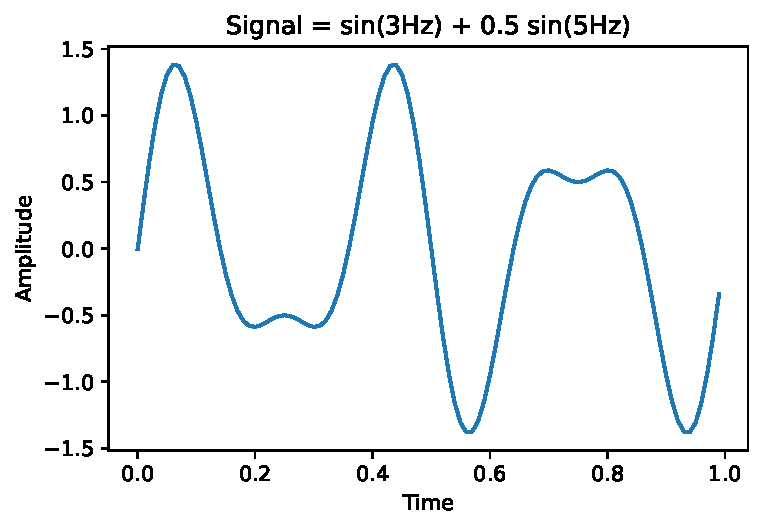
\includegraphics[keepaspectratio]{books/en-US/lab_files/figure-latex/cell-449-output-1.pdf}}

\begin{enumerate}
\def\labelenumi{\arabic{enumi}.}
\setcounter{enumi}{1}
\tightlist
\item
  Compute Fourier transform (DFT)
\end{enumerate}

\begin{Shaded}
\begin{Highlighting}[]
\NormalTok{X }\OperatorTok{=}\NormalTok{ np.fft.fft(signal)}
\NormalTok{freqs }\OperatorTok{=}\NormalTok{ np.fft.fftfreq(}\BuiltInTok{len}\NormalTok{(t), d}\OperatorTok{=}\DecValTok{1}\OperatorTok{/}\DecValTok{100}\NormalTok{)  }\CommentTok{\# sampling rate = 100Hz}

\NormalTok{plt.stem(freqs[:}\DecValTok{50}\NormalTok{], np.}\BuiltInTok{abs}\NormalTok{(X[:}\DecValTok{50}\NormalTok{]), basefmt}\OperatorTok{=}\StringTok{" "}\NormalTok{)}
\NormalTok{plt.title(}\StringTok{"Fourier spectrum"}\NormalTok{)}
\NormalTok{plt.xlabel(}\StringTok{"Frequency (Hz)"}\NormalTok{)}
\NormalTok{plt.ylabel(}\StringTok{"Magnitude"}\NormalTok{)}
\NormalTok{plt.show()}
\end{Highlighting}
\end{Shaded}

\pandocbounded{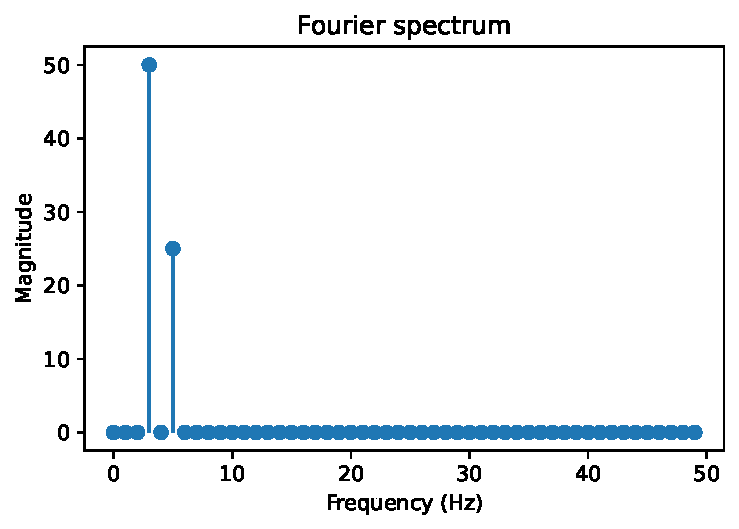
\includegraphics[keepaspectratio]{books/en-US/lab_files/figure-latex/cell-450-output-1.pdf}}

Peaks appear at 3Hz and 5Hz → the frequencies of the original signal.

\begin{enumerate}
\def\labelenumi{\arabic{enumi}.}
\setcounter{enumi}{2}
\tightlist
\item
  Reconstruct signal using inverse FFT
\end{enumerate}

\begin{Shaded}
\begin{Highlighting}[]
\NormalTok{signal\_reconstructed }\OperatorTok{=}\NormalTok{ np.fft.ifft(X).real}
\BuiltInTok{print}\NormalTok{(}\StringTok{"Reconstruction error:"}\NormalTok{, np.linalg.norm(signal }\OperatorTok{{-}}\NormalTok{ signal\_reconstructed))}
\end{Highlighting}
\end{Shaded}

\begin{verbatim}
Reconstruction error: 1.4664679821708477e-15
\end{verbatim}

Error is near zero → perfect reconstruction.

\begin{enumerate}
\def\labelenumi{\arabic{enumi}.}
\setcounter{enumi}{3}
\tightlist
\item
  Orthogonality check of sinusoids
\end{enumerate}

\begin{Shaded}
\begin{Highlighting}[]
\NormalTok{u }\OperatorTok{=}\NormalTok{ np.sin(}\DecValTok{2}\OperatorTok{*}\NormalTok{np.pi}\OperatorTok{*}\DecValTok{3}\OperatorTok{*}\NormalTok{t)}
\NormalTok{v }\OperatorTok{=}\NormalTok{ np.sin(}\DecValTok{2}\OperatorTok{*}\NormalTok{np.pi}\OperatorTok{*}\DecValTok{5}\OperatorTok{*}\NormalTok{t)}

\NormalTok{inner }\OperatorTok{=}\NormalTok{ np.dot(u, v)}
\BuiltInTok{print}\NormalTok{(}\StringTok{"Inner product of 3Hz and 5Hz sinusoids:"}\NormalTok{, inner)}
\end{Highlighting}
\end{Shaded}

\begin{verbatim}
Inner product of 3Hz and 5Hz sinusoids: 1.2961853812498703e-14
\end{verbatim}

The result is ≈ 0 → confirms orthogonality.

\subsubsection{Try It Yourself}\label{try-it-yourself-177}

\begin{enumerate}
\def\labelenumi{\arabic{enumi}.}
\tightlist
\item
  Change the frequencies to 7Hz and 9Hz. Do the Fourier peaks move
  accordingly?
\item
  Mix in some noise and check how the spectrum looks.
\item
  Try cosine signals instead of sine. Do you still see orthogonality?
\end{enumerate}

\subsubsection{The Takeaway}\label{the-takeaway-61}

\begin{itemize}
\tightlist
\item
  Fourier analysis = linear algebra with orthogonal sinusoidal basis
  functions.
\item
  Any signal can be decomposed into orthogonal waves.
\item
  This orthogonal viewpoint powers audio, image compression, and signal
  processing.
\end{itemize}

\subsection{80. Polynomial and Multifeature Least Squares (Fitting More
Flexibly)}\label{polynomial-and-multifeature-least-squares-fitting-more-flexibly}

Least squares isn't limited to straight lines. By adding polynomial or
multiple features, we can fit curves and capture more complex
relationships. This is the foundation of regression models in data
science.

\subsubsection{Formula Recap}\label{formula-recap-2}

Given data \((x_i, y_i)\), we build a design matrix \(A\):

\begin{itemize}
\tightlist
\item
  For polynomial fit of degree \(d\):
\end{itemize}

\[
A = \begin{bmatrix}
1 & x_1 & x_1^2 & \dots & x_1^d \\
1 & x_2 & x_2^2 & \dots & x_2^d \\
\vdots & \vdots & \vdots & \ddots & \vdots \\
1 & x_n & x_n^2 & \dots & x_n^d
\end{bmatrix}
\]

Then solve least squares:

\[
\hat{c} = \arg\min_c \|Ac - y\|^2
\]

\subsubsection{Set Up Your Lab}\label{set-up-your-lab-79}

\begin{Shaded}
\begin{Highlighting}[]
\ImportTok{import}\NormalTok{ numpy }\ImportTok{as}\NormalTok{ np}
\ImportTok{import}\NormalTok{ matplotlib.pyplot }\ImportTok{as}\NormalTok{ plt}
\end{Highlighting}
\end{Shaded}

\subsubsection{Step-by-Step Code
Walkthrough}\label{step-by-step-code-walkthrough-79}

\begin{enumerate}
\def\labelenumi{\arabic{enumi}.}
\tightlist
\item
  Generate noisy quadratic data
\end{enumerate}

\begin{Shaded}
\begin{Highlighting}[]
\NormalTok{np.random.seed(}\DecValTok{0}\NormalTok{)}
\NormalTok{x }\OperatorTok{=}\NormalTok{ np.linspace(}\OperatorTok{{-}}\DecValTok{3}\NormalTok{, }\DecValTok{3}\NormalTok{, }\DecValTok{30}\NormalTok{)}
\NormalTok{y\_true }\OperatorTok{=} \DecValTok{1} \OperatorTok{{-}} \DecValTok{2}\OperatorTok{*}\NormalTok{x }\OperatorTok{+} \FloatTok{0.5}\OperatorTok{*}\NormalTok{x}\OperatorTok{**}\DecValTok{2}
\NormalTok{y\_noisy }\OperatorTok{=}\NormalTok{ y\_true }\OperatorTok{+}\NormalTok{ np.random.normal(scale}\OperatorTok{=}\FloatTok{2.0}\NormalTok{, size}\OperatorTok{=}\NormalTok{x.shape)}

\NormalTok{plt.scatter(x, y\_noisy, label}\OperatorTok{=}\StringTok{"Noisy data"}\NormalTok{)}
\NormalTok{plt.plot(x, y\_true, }\StringTok{"g{-}{-}"}\NormalTok{, label}\OperatorTok{=}\StringTok{"True curve"}\NormalTok{)}
\NormalTok{plt.legend()}
\NormalTok{plt.show()}
\end{Highlighting}
\end{Shaded}

\pandocbounded{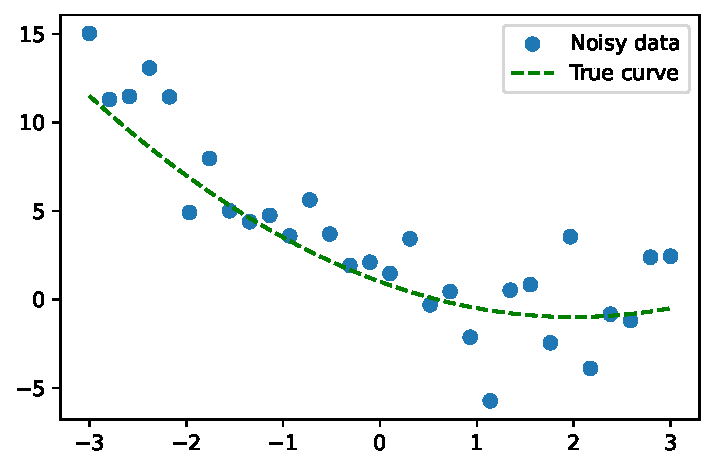
\includegraphics[keepaspectratio]{books/en-US/lab_files/figure-latex/cell-454-output-1.pdf}}

\begin{enumerate}
\def\labelenumi{\arabic{enumi}.}
\setcounter{enumi}{1}
\tightlist
\item
  Build polynomial design matrix (degree 2)
\end{enumerate}

\begin{Shaded}
\begin{Highlighting}[]
\NormalTok{A }\OperatorTok{=}\NormalTok{ np.column\_stack([np.ones\_like(x), x, x}\OperatorTok{**}\DecValTok{2}\NormalTok{])}
\NormalTok{coeffs, }\OperatorTok{*}\NormalTok{\_ }\OperatorTok{=}\NormalTok{ np.linalg.lstsq(A, y\_noisy, rcond}\OperatorTok{=}\VariableTok{None}\NormalTok{)}
\BuiltInTok{print}\NormalTok{(}\StringTok{"Fitted coefficients:"}\NormalTok{, coeffs)}
\end{Highlighting}
\end{Shaded}

\begin{verbatim}
Fitted coefficients: [ 1.15666306 -2.25753954  0.72733812]
\end{verbatim}

\begin{enumerate}
\def\labelenumi{\arabic{enumi}.}
\setcounter{enumi}{2}
\tightlist
\item
  Plot fitted polynomial
\end{enumerate}

\begin{Shaded}
\begin{Highlighting}[]
\NormalTok{y\_fit }\OperatorTok{=}\NormalTok{ A }\OperatorTok{@}\NormalTok{ coeffs}
\NormalTok{plt.scatter(x, y\_noisy, label}\OperatorTok{=}\StringTok{"Noisy data"}\NormalTok{)}
\NormalTok{plt.plot(x, y\_fit, }\StringTok{"r{-}"}\NormalTok{, label}\OperatorTok{=}\StringTok{"Fitted quadratic"}\NormalTok{)}
\NormalTok{plt.legend()}
\NormalTok{plt.show()}
\end{Highlighting}
\end{Shaded}

\pandocbounded{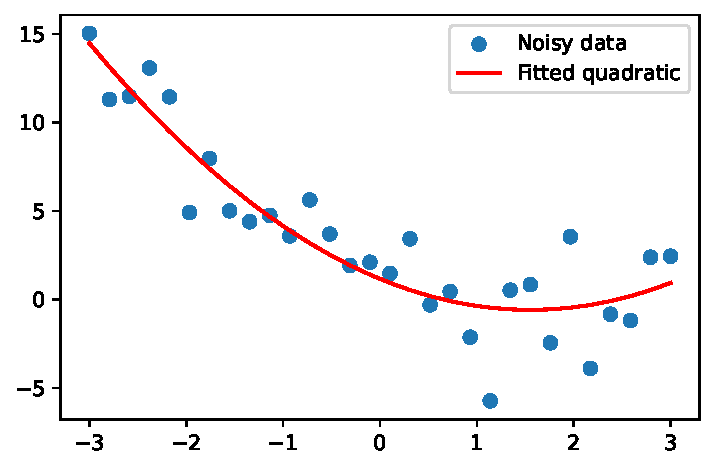
\includegraphics[keepaspectratio]{books/en-US/lab_files/figure-latex/cell-456-output-1.pdf}}

\begin{enumerate}
\def\labelenumi{\arabic{enumi}.}
\setcounter{enumi}{3}
\tightlist
\item
  Higher-degree fit (overfitting demonstration)
\end{enumerate}

\begin{Shaded}
\begin{Highlighting}[]
\NormalTok{A\_high }\OperatorTok{=}\NormalTok{ np.column\_stack([x}\OperatorTok{**}\NormalTok{i }\ControlFlowTok{for}\NormalTok{ i }\KeywordTok{in} \BuiltInTok{range}\NormalTok{(}\DecValTok{6}\NormalTok{)])  }\CommentTok{\# degree 5}
\NormalTok{coeffs\_high, }\OperatorTok{*}\NormalTok{\_ }\OperatorTok{=}\NormalTok{ np.linalg.lstsq(A\_high, y\_noisy, rcond}\OperatorTok{=}\VariableTok{None}\NormalTok{)}

\NormalTok{y\_fit\_high }\OperatorTok{=}\NormalTok{ A\_high }\OperatorTok{@}\NormalTok{ coeffs\_high}
\NormalTok{plt.scatter(x, y\_noisy, label}\OperatorTok{=}\StringTok{"Noisy data"}\NormalTok{)}
\NormalTok{plt.plot(x, y\_fit\_high, }\StringTok{"r{-}"}\NormalTok{, label}\OperatorTok{=}\StringTok{"Degree 5 polynomial"}\NormalTok{)}
\NormalTok{plt.plot(x, y\_true, }\StringTok{"g{-}{-}"}\NormalTok{, label}\OperatorTok{=}\StringTok{"True curve"}\NormalTok{)}
\NormalTok{plt.legend()}
\NormalTok{plt.show()}
\end{Highlighting}
\end{Shaded}

\pandocbounded{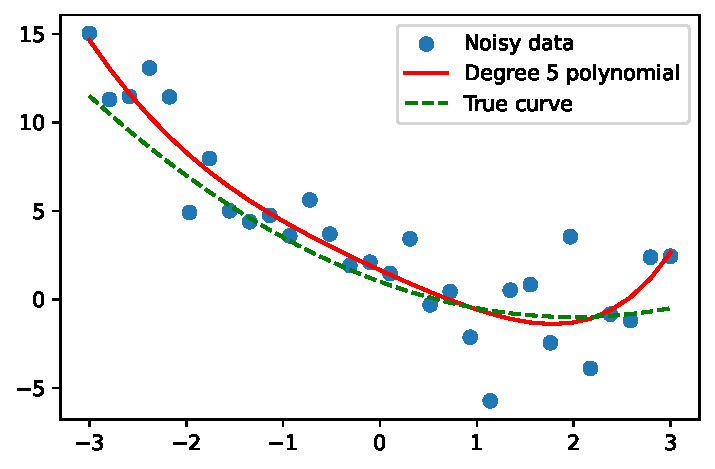
\includegraphics[keepaspectratio]{books/en-US/lab_files/figure-latex/cell-457-output-1.pdf}}

\begin{enumerate}
\def\labelenumi{\arabic{enumi}.}
\setcounter{enumi}{4}
\tightlist
\item
  Multifeature regression example
\end{enumerate}

Suppose we predict \(y\) from features \([x, x^2, \sin(x)]\):

\begin{Shaded}
\begin{Highlighting}[]
\NormalTok{A\_multi }\OperatorTok{=}\NormalTok{ np.column\_stack([np.ones\_like(x), x, x}\OperatorTok{**}\DecValTok{2}\NormalTok{, np.sin(x)])}
\NormalTok{coeffs\_multi, }\OperatorTok{*}\NormalTok{\_ }\OperatorTok{=}\NormalTok{ np.linalg.lstsq(A\_multi, y\_noisy, rcond}\OperatorTok{=}\VariableTok{None}\NormalTok{)}
\BuiltInTok{print}\NormalTok{(}\StringTok{"Multi{-}feature coefficients:"}\NormalTok{, coeffs\_multi)}
\end{Highlighting}
\end{Shaded}

\begin{verbatim}
Multi-feature coefficients: [ 1.15666306 -2.0492999   0.72733812 -0.65902274]
\end{verbatim}

\subsubsection{Try It Yourself}\label{try-it-yourself-178}

\begin{enumerate}
\def\labelenumi{\arabic{enumi}.}
\tightlist
\item
  Fit degree 3, 4, 5 polynomials to the same data. Watch how the curve
  changes.
\item
  Add features like \(\cos(x)\) or \(\exp(x)\) - does the fit improve?
\item
  Compare training error (fit to noisy data) vs error on new test
  points.
\end{enumerate}

\subsubsection{The Takeaway}\label{the-takeaway-62}

\begin{itemize}
\tightlist
\item
  Least squares can fit polynomials and arbitrary feature combinations.
\item
  The design matrix encodes how input variables transform into features.
\item
  This is the basis of regression, curve fitting, and many machine
  learning models.
\end{itemize}

\section{Chapter 9. SVD, PCA, and
Conditioning}\label{chapter-9.-svd-pca-and-conditioning-2}

\subsection{81. Singular Values and SVD (Universal
Factorization)}\label{singular-values-and-svd-universal-factorization}

The Singular Value Decomposition (SVD) is one of the most powerful
results in linear algebra. It says any \(m \times n\) matrix \(A\) can
be factored as:

\[
A = U \Sigma V^T
\]

\begin{itemize}
\tightlist
\item
  \(U\): orthogonal \(m \times m\) matrix (left singular vectors)
\item
  \(\Sigma\): diagonal \(m \times n\) matrix with nonnegative numbers
  (singular values)
\item
  \(V\): orthogonal \(n \times n\) matrix (right singular vectors)
\end{itemize}

Singular values are always nonnegative and sorted
\(\sigma_1 \geq \sigma_2 \geq \dots\).

\subsubsection{Set Up Your Lab}\label{set-up-your-lab-80}

\begin{Shaded}
\begin{Highlighting}[]
\ImportTok{import}\NormalTok{ numpy }\ImportTok{as}\NormalTok{ np}
\end{Highlighting}
\end{Shaded}

\subsubsection{Step-by-Step Code
Walkthrough}\label{step-by-step-code-walkthrough-80}

\begin{enumerate}
\def\labelenumi{\arabic{enumi}.}
\tightlist
\item
  Compute SVD of a matrix
\end{enumerate}

\begin{Shaded}
\begin{Highlighting}[]
\NormalTok{A }\OperatorTok{=}\NormalTok{ np.array([[}\DecValTok{3}\NormalTok{,}\DecValTok{1}\NormalTok{,}\DecValTok{1}\NormalTok{],}
\NormalTok{              [}\OperatorTok{{-}}\DecValTok{1}\NormalTok{,}\DecValTok{3}\NormalTok{,}\DecValTok{1}\NormalTok{]])}

\NormalTok{U, S, Vt }\OperatorTok{=}\NormalTok{ np.linalg.svd(A, full\_matrices}\OperatorTok{=}\VariableTok{True}\NormalTok{)}

\BuiltInTok{print}\NormalTok{(}\StringTok{"U:}\CharTok{\textbackslash{}n}\StringTok{"}\NormalTok{, U)}
\BuiltInTok{print}\NormalTok{(}\StringTok{"Singular values:"}\NormalTok{, S)}
\BuiltInTok{print}\NormalTok{(}\StringTok{"V\^{}T:}\CharTok{\textbackslash{}n}\StringTok{"}\NormalTok{, Vt)}
\end{Highlighting}
\end{Shaded}

\begin{verbatim}
U:
 [[-0.70710678 -0.70710678]
 [-0.70710678  0.70710678]]
Singular values: [3.46410162 3.16227766]
V^T:
 [[-4.08248290e-01 -8.16496581e-01 -4.08248290e-01]
 [-8.94427191e-01  4.47213595e-01  5.27355937e-16]
 [-1.82574186e-01 -3.65148372e-01  9.12870929e-01]]
\end{verbatim}

\begin{itemize}
\tightlist
\item
  \texttt{U}: orthogonal basis in input space.
\item
  \texttt{S}: singular values (as a 1D array).
\item
  \texttt{V\^{}T}: orthogonal basis in output space.
\end{itemize}

\begin{enumerate}
\def\labelenumi{\arabic{enumi}.}
\setcounter{enumi}{1}
\tightlist
\item
  Reconstruct \(A\) from decomposition
\end{enumerate}

\begin{Shaded}
\begin{Highlighting}[]
\NormalTok{Sigma }\OperatorTok{=}\NormalTok{ np.zeros((U.shape[}\DecValTok{1}\NormalTok{], Vt.shape[}\DecValTok{0}\NormalTok{]))}
\NormalTok{Sigma[:}\BuiltInTok{len}\NormalTok{(S), :}\BuiltInTok{len}\NormalTok{(S)] }\OperatorTok{=}\NormalTok{ np.diag(S)}

\NormalTok{A\_reconstructed }\OperatorTok{=}\NormalTok{ U }\OperatorTok{@}\NormalTok{ Sigma }\OperatorTok{@}\NormalTok{ Vt}
\BuiltInTok{print}\NormalTok{(}\StringTok{"Reconstruction error:"}\NormalTok{, np.linalg.norm(A }\OperatorTok{{-}}\NormalTok{ A\_reconstructed))}
\end{Highlighting}
\end{Shaded}

\begin{verbatim}
Reconstruction error: 1.5895974606912448e-15
\end{verbatim}

The error should be near zero.

\begin{enumerate}
\def\labelenumi{\arabic{enumi}.}
\setcounter{enumi}{2}
\tightlist
\item
  Rank from SVD
\end{enumerate}

Number of nonzero singular values = rank of \(A\).

\begin{Shaded}
\begin{Highlighting}[]
\NormalTok{rank }\OperatorTok{=}\NormalTok{ np.}\BuiltInTok{sum}\NormalTok{(S }\OperatorTok{\textgreater{}} \FloatTok{1e{-}10}\NormalTok{)}
\BuiltInTok{print}\NormalTok{(}\StringTok{"Rank of A:"}\NormalTok{, rank)}
\end{Highlighting}
\end{Shaded}

\begin{verbatim}
Rank of A: 2
\end{verbatim}

\begin{enumerate}
\def\labelenumi{\arabic{enumi}.}
\setcounter{enumi}{3}
\tightlist
\item
  Geometry: effect of \(A\)
\end{enumerate}

SVD says:

\begin{enumerate}
\def\labelenumi{\arabic{enumi}.}
\tightlist
\item
  \(V\) rotates input space.
\item
  \(\Sigma\) scales along orthogonal directions (by singular values).
\item
  \(U\) rotates to output space.
\end{enumerate}

This explains why SVD works for any matrix (not just square ones).

\begin{enumerate}
\def\labelenumi{\arabic{enumi}.}
\setcounter{enumi}{4}
\tightlist
\item
  Low-rank approximation preview
\end{enumerate}

Keep only the top singular value(s) → best approximation of \(A\).

\begin{Shaded}
\begin{Highlighting}[]
\NormalTok{k }\OperatorTok{=} \DecValTok{1}
\NormalTok{A\_approx }\OperatorTok{=}\NormalTok{ np.outer(U[:,}\DecValTok{0}\NormalTok{], Vt[}\DecValTok{0}\NormalTok{]) }\OperatorTok{*}\NormalTok{ S[}\DecValTok{0}\NormalTok{]}
\BuiltInTok{print}\NormalTok{(}\StringTok{"Rank{-}1 approximation:}\CharTok{\textbackslash{}n}\StringTok{"}\NormalTok{, A\_approx)}
\end{Highlighting}
\end{Shaded}

\begin{verbatim}
Rank-1 approximation:
 [[1. 2. 1.]
 [1. 2. 1.]]
\end{verbatim}

\subsubsection{Try It Yourself}\label{try-it-yourself-179}

\begin{enumerate}
\def\labelenumi{\arabic{enumi}.}
\tightlist
\item
  Compute SVD for a random 5×3 matrix. Check if \(U\) and \(V\) are
  orthogonal.
\item
  Compare singular values of a diagonal matrix vs a rotation matrix.
\item
  Zero out small singular values and see how much of \(A\) is preserved.
\end{enumerate}

\subsubsection{The Takeaway}\label{the-takeaway-63}

\begin{itemize}
\tightlist
\item
  SVD factorizes any matrix into rotations and scalings.
\item
  Singular values reveal rank and strength of directions.
\item
  It's the universal tool of numerical linear algebra: the backbone of
  PCA, compression, and stability analysis.
\end{itemize}

\subsection{82. Geometry of SVD (Rotations +
Stretching)}\label{geometry-of-svd-rotations-stretching}

The Singular Value Decomposition (SVD) has a beautiful geometric
interpretation: every matrix is just a combination of two rotations (or
reflections) and a stretching.

For \(A = U \Sigma V^T\):

\begin{enumerate}
\def\labelenumi{\arabic{enumi}.}
\tightlist
\item
  \(V^T\): rotates (or reflects) the input space.
\item
  \(\Sigma\): stretches space along orthogonal axes by singular values
  \(\sigma_i\).
\item
  \(U\): rotates (or reflects) the result into the output space.
\end{enumerate}

This turns any linear transformation into a rotation → stretching →
rotation pipeline.

\subsubsection{Set Up Your Lab}\label{set-up-your-lab-81}

\begin{Shaded}
\begin{Highlighting}[]
\ImportTok{import}\NormalTok{ numpy }\ImportTok{as}\NormalTok{ np}
\ImportTok{import}\NormalTok{ matplotlib.pyplot }\ImportTok{as}\NormalTok{ plt}
\end{Highlighting}
\end{Shaded}

\subsubsection{Step-by-Step Code
Walkthrough}\label{step-by-step-code-walkthrough-81}

\begin{enumerate}
\def\labelenumi{\arabic{enumi}.}
\tightlist
\item
  Make a 2D matrix
\end{enumerate}

\begin{Shaded}
\begin{Highlighting}[]
\NormalTok{A }\OperatorTok{=}\NormalTok{ np.array([[}\DecValTok{2}\NormalTok{, }\DecValTok{1}\NormalTok{],}
\NormalTok{              [}\DecValTok{1}\NormalTok{, }\DecValTok{3}\NormalTok{]])}
\end{Highlighting}
\end{Shaded}

\begin{enumerate}
\def\labelenumi{\arabic{enumi}.}
\setcounter{enumi}{1}
\tightlist
\item
  Apply SVD
\end{enumerate}

\begin{Shaded}
\begin{Highlighting}[]
\NormalTok{U, S, Vt }\OperatorTok{=}\NormalTok{ np.linalg.svd(A)}

\BuiltInTok{print}\NormalTok{(}\StringTok{"U:}\CharTok{\textbackslash{}n}\StringTok{"}\NormalTok{, U)}
\BuiltInTok{print}\NormalTok{(}\StringTok{"Singular values:"}\NormalTok{, S)}
\BuiltInTok{print}\NormalTok{(}\StringTok{"V\^{}T:}\CharTok{\textbackslash{}n}\StringTok{"}\NormalTok{, Vt)}
\end{Highlighting}
\end{Shaded}

\begin{verbatim}
U:
 [[-0.52573111 -0.85065081]
 [-0.85065081  0.52573111]]
Singular values: [3.61803399 1.38196601]
V^T:
 [[-0.52573111 -0.85065081]
 [-0.85065081  0.52573111]]
\end{verbatim}

\begin{enumerate}
\def\labelenumi{\arabic{enumi}.}
\setcounter{enumi}{2}
\tightlist
\item
  Visualize effect on the unit circle
\end{enumerate}

The unit circle is often used to visualize linear transformations.

\begin{Shaded}
\begin{Highlighting}[]
\NormalTok{theta }\OperatorTok{=}\NormalTok{ np.linspace(}\DecValTok{0}\NormalTok{, }\DecValTok{2}\OperatorTok{*}\NormalTok{np.pi, }\DecValTok{200}\NormalTok{)}
\NormalTok{circle }\OperatorTok{=}\NormalTok{ np.vstack((np.cos(theta), np.sin(theta)))}

\NormalTok{transformed }\OperatorTok{=}\NormalTok{ A }\OperatorTok{@}\NormalTok{ circle}

\NormalTok{plt.plot(circle[}\DecValTok{0}\NormalTok{], circle[}\DecValTok{1}\NormalTok{], }\StringTok{\textquotesingle{}b{-}{-}\textquotesingle{}}\NormalTok{, label}\OperatorTok{=}\StringTok{"Unit circle"}\NormalTok{)}
\NormalTok{plt.plot(transformed[}\DecValTok{0}\NormalTok{], transformed[}\DecValTok{1}\NormalTok{], }\StringTok{\textquotesingle{}r{-}\textquotesingle{}}\NormalTok{, label}\OperatorTok{=}\StringTok{"Transformed"}\NormalTok{)}
\NormalTok{plt.axis(}\StringTok{"equal"}\NormalTok{)}
\NormalTok{plt.legend()}
\NormalTok{plt.title(}\StringTok{"Action of A on the unit circle"}\NormalTok{)}
\NormalTok{plt.show()}
\end{Highlighting}
\end{Shaded}

\pandocbounded{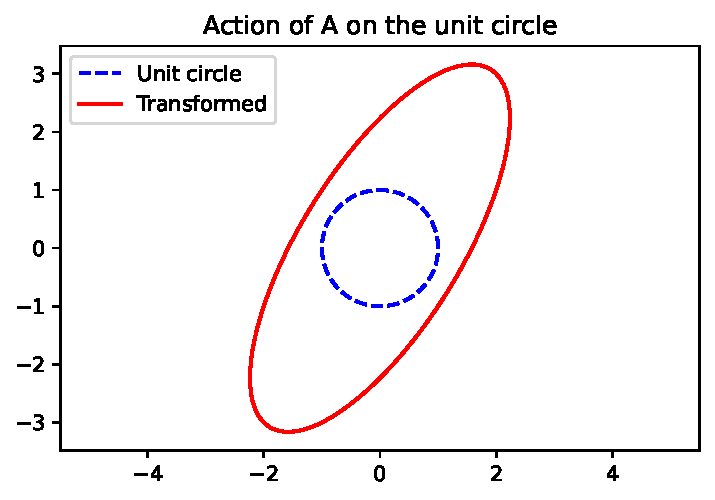
\includegraphics[keepaspectratio]{books/en-US/lab_files/figure-latex/cell-467-output-1.pdf}}

The circle becomes an ellipse. Its axes align with the singular vectors,
and its radii are the singular values.

\begin{enumerate}
\def\labelenumi{\arabic{enumi}.}
\setcounter{enumi}{3}
\tightlist
\item
  Compare with decomposition steps
\end{enumerate}

\begin{Shaded}
\begin{Highlighting}[]
\CommentTok{\# Apply V\^{}T}
\NormalTok{step1 }\OperatorTok{=}\NormalTok{ Vt }\OperatorTok{@}\NormalTok{ circle}
\CommentTok{\# Apply Σ}
\NormalTok{Sigma }\OperatorTok{=}\NormalTok{ np.diag(S)}
\NormalTok{step2 }\OperatorTok{=}\NormalTok{ Sigma }\OperatorTok{@}\NormalTok{ step1}
\CommentTok{\# Apply U}
\NormalTok{step3 }\OperatorTok{=}\NormalTok{ U }\OperatorTok{@}\NormalTok{ step2}

\NormalTok{plt.plot(circle[}\DecValTok{0}\NormalTok{], circle[}\DecValTok{1}\NormalTok{], }\StringTok{\textquotesingle{}b{-}{-}\textquotesingle{}}\NormalTok{, label}\OperatorTok{=}\StringTok{"Unit circle"}\NormalTok{)}
\NormalTok{plt.plot(step3[}\DecValTok{0}\NormalTok{], step3[}\DecValTok{1}\NormalTok{], }\StringTok{\textquotesingle{}g{-}\textquotesingle{}}\NormalTok{, label}\OperatorTok{=}\StringTok{"U Σ V\^{}T circle"}\NormalTok{)}
\NormalTok{plt.axis(}\StringTok{"equal"}\NormalTok{)}
\NormalTok{plt.legend()}
\NormalTok{plt.title(}\StringTok{"SVD decomposition of transformation"}\NormalTok{)}
\NormalTok{plt.show()}
\end{Highlighting}
\end{Shaded}

\pandocbounded{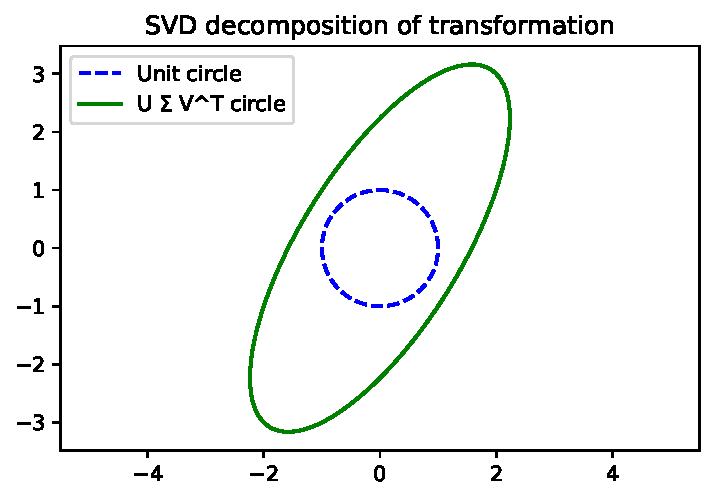
\includegraphics[keepaspectratio]{books/en-US/lab_files/figure-latex/cell-468-output-1.pdf}}

Both transformed shapes match → confirms SVD's geometric picture.

\subsubsection{Try It Yourself}\label{try-it-yourself-180}

\begin{enumerate}
\def\labelenumi{\arabic{enumi}.}
\tightlist
\item
  Change \(A\) to a pure shear, like \texttt{{[}{[}1,2{]},{[}0,1{]}{]}}.
  How does the ellipse look?
\item
  Try a diagonal matrix, like \texttt{{[}{[}3,0{]},{[}0,1{]}{]}}. Do the
  singular vectors match the coordinate axes?
\item
  Scale the input circle to a square and see if geometry still works.
\end{enumerate}

\subsubsection{The Takeaway}\label{the-takeaway-64}

\begin{itemize}
\tightlist
\item
  SVD = rotate → stretch → rotate.
\item
  The unit circle becomes an ellipse: axes = singular vectors, radii =
  singular values.
\item
  This geometric lens makes SVD intuitive and explains why it's so
  widely used in data, graphics, and signal processing.
\end{itemize}

\subsection{83. Relation to Eigen-Decompositions (ATA and
AAT)}\label{relation-to-eigen-decompositions-ata-and-aat}

Singular values and eigenvalues are closely connected. While
eigen-decomposition applies only to square matrices, SVD works for any
rectangular matrix. The bridge between them is:

\[
A^T A v = \sigma^2 v \quad \text{and} \quad A A^T u = \sigma^2 u
\]

\begin{itemize}
\tightlist
\item
  \(v\): right singular vector (from eigenvectors of \(A^T A\))
\item
  \(u\): left singular vector (from eigenvectors of \(A A^T\))
\item
  \(\sigma\): singular values (square roots of eigenvalues of \(A^T A\)
  or \(A A^T\))
\end{itemize}

\subsubsection{Set Up Your Lab}\label{set-up-your-lab-82}

\begin{Shaded}
\begin{Highlighting}[]
\ImportTok{import}\NormalTok{ numpy }\ImportTok{as}\NormalTok{ np}
\end{Highlighting}
\end{Shaded}

\subsubsection{Step-by-Step Code
Walkthrough}\label{step-by-step-code-walkthrough-82}

\begin{enumerate}
\def\labelenumi{\arabic{enumi}.}
\tightlist
\item
  Define a rectangular matrix
\end{enumerate}

\begin{Shaded}
\begin{Highlighting}[]
\NormalTok{A }\OperatorTok{=}\NormalTok{ np.array([[}\DecValTok{2}\NormalTok{, }\DecValTok{0}\NormalTok{],}
\NormalTok{              [}\DecValTok{1}\NormalTok{, }\DecValTok{1}\NormalTok{],}
\NormalTok{              [}\DecValTok{0}\NormalTok{, }\DecValTok{1}\NormalTok{]])  }\CommentTok{\# shape 3x2}
\end{Highlighting}
\end{Shaded}

\begin{enumerate}
\def\labelenumi{\arabic{enumi}.}
\setcounter{enumi}{1}
\tightlist
\item
  Compute SVD directly
\end{enumerate}

\begin{Shaded}
\begin{Highlighting}[]
\NormalTok{U, S, Vt }\OperatorTok{=}\NormalTok{ np.linalg.svd(A)}
\BuiltInTok{print}\NormalTok{(}\StringTok{"Singular values:"}\NormalTok{, S)}
\end{Highlighting}
\end{Shaded}

\begin{verbatim}
Singular values: [2.30277564 1.30277564]
\end{verbatim}

\begin{enumerate}
\def\labelenumi{\arabic{enumi}.}
\setcounter{enumi}{2}
\tightlist
\item
  Compare with eigenvalues of \(A^T A\)
\end{enumerate}

\begin{Shaded}
\begin{Highlighting}[]
\NormalTok{ATA }\OperatorTok{=}\NormalTok{ A.T }\OperatorTok{@}\NormalTok{ A}
\NormalTok{eigvals, eigvecs }\OperatorTok{=}\NormalTok{ np.linalg.eig(ATA)}

\BuiltInTok{print}\NormalTok{(}\StringTok{"Eigenvalues of A\^{}T A:"}\NormalTok{, eigvals)}
\BuiltInTok{print}\NormalTok{(}\StringTok{"Square roots (sorted):"}\NormalTok{, np.sqrt(np.sort(eigvals)[::}\OperatorTok{{-}}\DecValTok{1}\NormalTok{]))}
\end{Highlighting}
\end{Shaded}

\begin{verbatim}
Eigenvalues of A^T A: [5.30277564 1.69722436]
Square roots (sorted): [2.30277564 1.30277564]
\end{verbatim}

Notice: singular values from SVD = square roots of eigenvalues of
\(A^T A\).

\begin{enumerate}
\def\labelenumi{\arabic{enumi}.}
\setcounter{enumi}{3}
\tightlist
\item
  Compare with eigenvalues of \(A A^T\)
\end{enumerate}

\begin{Shaded}
\begin{Highlighting}[]
\NormalTok{AAT }\OperatorTok{=}\NormalTok{ A }\OperatorTok{@}\NormalTok{ A.T}
\NormalTok{eigvals2, eigvecs2 }\OperatorTok{=}\NormalTok{ np.linalg.eig(AAT)}

\BuiltInTok{print}\NormalTok{(}\StringTok{"Eigenvalues of A A\^{}T:"}\NormalTok{, eigvals2)}
\BuiltInTok{print}\NormalTok{(}\StringTok{"Square roots:"}\NormalTok{, np.sqrt(np.sort(eigvals2)[::}\OperatorTok{{-}}\DecValTok{1}\NormalTok{]))}
\end{Highlighting}
\end{Shaded}

\begin{verbatim}
Eigenvalues of A A^T: [ 5.30277564e+00  1.69722436e+00 -2.01266546e-17]
Square roots: [2.30277564 1.30277564        nan]
\end{verbatim}

\begin{verbatim}
/var/folders/_g/lq_pglm508df70x751kkxrl80000gp/T/ipykernel_31637/436251338.py:5: RuntimeWarning: invalid value encountered in sqrt
  print("Square roots:", np.sqrt(np.sort(eigvals2)[::-1]))
\end{verbatim}

They match too → confirming the relationship.

\begin{enumerate}
\def\labelenumi{\arabic{enumi}.}
\setcounter{enumi}{4}
\tightlist
\item
  Verify singular vectors
\end{enumerate}

\begin{itemize}
\tightlist
\item
  Right singular vectors (\(V\)) = eigenvectors of \(A^T A\).
\item
  Left singular vectors (\(U\)) = eigenvectors of \(A A^T\).
\end{itemize}

\begin{Shaded}
\begin{Highlighting}[]
\BuiltInTok{print}\NormalTok{(}\StringTok{"Right singular vectors (V):}\CharTok{\textbackslash{}n}\StringTok{"}\NormalTok{, Vt.T)}
\BuiltInTok{print}\NormalTok{(}\StringTok{"Eigenvectors of A\^{}T A:}\CharTok{\textbackslash{}n}\StringTok{"}\NormalTok{, eigvecs)}

\BuiltInTok{print}\NormalTok{(}\StringTok{"Left singular vectors (U):}\CharTok{\textbackslash{}n}\StringTok{"}\NormalTok{, U)}
\BuiltInTok{print}\NormalTok{(}\StringTok{"Eigenvectors of A A\^{}T:}\CharTok{\textbackslash{}n}\StringTok{"}\NormalTok{, eigvecs2)}
\end{Highlighting}
\end{Shaded}

\begin{verbatim}
Right singular vectors (V):
 [[-0.95709203  0.28978415]
 [-0.28978415 -0.95709203]]
Eigenvectors of A^T A:
 [[ 0.95709203 -0.28978415]
 [ 0.28978415  0.95709203]]
Left singular vectors (U):
 [[-0.83125078  0.44487192  0.33333333]
 [-0.54146663 -0.51222011 -0.66666667]
 [-0.12584124 -0.73465607  0.66666667]]
Eigenvectors of A A^T:
 [[-0.83125078  0.44487192  0.33333333]
 [-0.54146663 -0.51222011 -0.66666667]
 [-0.12584124 -0.73465607  0.66666667]]
\end{verbatim}

\subsubsection{Try It Yourself}\label{try-it-yourself-181}

\begin{enumerate}
\def\labelenumi{\arabic{enumi}.}
\tightlist
\item
  Try a square symmetric matrix and compare SVD with
  eigen-decomposition. Do they match?
\item
  For a tall vs wide rectangular matrix, check whether \(U\) and \(V\)
  differ.
\item
  Compute eigenvalues manually with \texttt{np.linalg.eig} for a random
  \(A\) and confirm singular values.
\end{enumerate}

\subsubsection{The Takeaway}\label{the-takeaway-65}

\begin{itemize}
\tightlist
\item
  Singular values = square roots of eigenvalues of \(A^T A\) (or
  \(A A^T\)).
\item
  Right singular vectors = eigenvectors of \(A^T A\).
\item
  Left singular vectors = eigenvectors of \(A A^T\).
\item
  SVD generalizes eigen-decomposition to all matrices, rectangular or
  square.
\end{itemize}

\subsection{84. Low-Rank Approximation (Best Small
Models)}\label{low-rank-approximation-best-small-models-1}

One of the most useful applications of SVD is low-rank approximation:
compressing a large matrix into a smaller one while keeping most of the
important information.

The Eckart--Young theorem says: If \(A = U \Sigma V^T\), then the best
rank-\(k\) approximation (in least-squares sense) is:

\[
A_k = U_k \Sigma_k V_k^T
\]

where we keep only the top \(k\) singular values (and corresponding
vectors).

\subsubsection{Set Up Your Lab}\label{set-up-your-lab-83}

\begin{Shaded}
\begin{Highlighting}[]
\ImportTok{import}\NormalTok{ numpy }\ImportTok{as}\NormalTok{ np}
\ImportTok{import}\NormalTok{ matplotlib.pyplot }\ImportTok{as}\NormalTok{ plt}
\end{Highlighting}
\end{Shaded}

\subsubsection{Step-by-Step Code
Walkthrough}\label{step-by-step-code-walkthrough-83}

\begin{enumerate}
\def\labelenumi{\arabic{enumi}.}
\tightlist
\item
  Create a matrix with hidden low-rank structure
\end{enumerate}

\begin{Shaded}
\begin{Highlighting}[]
\NormalTok{np.random.seed(}\DecValTok{0}\NormalTok{)}
\NormalTok{U }\OperatorTok{=}\NormalTok{ np.random.randn(}\DecValTok{50}\NormalTok{, }\DecValTok{5}\NormalTok{)   }\CommentTok{\# 50 x 5}
\NormalTok{V }\OperatorTok{=}\NormalTok{ np.random.randn(}\DecValTok{5}\NormalTok{, }\DecValTok{30}\NormalTok{)   }\CommentTok{\# 5 x 30}
\NormalTok{A }\OperatorTok{=}\NormalTok{ U }\OperatorTok{@}\NormalTok{ V  }\CommentTok{\# true rank ≤ 5}
\end{Highlighting}
\end{Shaded}

\begin{enumerate}
\def\labelenumi{\arabic{enumi}.}
\setcounter{enumi}{1}
\tightlist
\item
  Full SVD
\end{enumerate}

\begin{Shaded}
\begin{Highlighting}[]
\NormalTok{U, S, Vt }\OperatorTok{=}\NormalTok{ np.linalg.svd(A, full\_matrices}\OperatorTok{=}\VariableTok{False}\NormalTok{)}
\BuiltInTok{print}\NormalTok{(}\StringTok{"Singular values:"}\NormalTok{, S[:}\DecValTok{10}\NormalTok{])}
\end{Highlighting}
\end{Shaded}

\begin{verbatim}
Singular values: [4.90672194e+01 4.05935057e+01 3.39228766e+01 3.07883338e+01
 2.29261740e+01 3.97150036e-15 3.97150036e-15 3.97150036e-15
 3.97150036e-15 3.97150036e-15]
\end{verbatim}

Only the first \textasciitilde5 should be large; the rest close to zero.

\begin{enumerate}
\def\labelenumi{\arabic{enumi}.}
\setcounter{enumi}{2}
\tightlist
\item
  Build rank-1 approximation
\end{enumerate}

\begin{Shaded}
\begin{Highlighting}[]
\NormalTok{k }\OperatorTok{=} \DecValTok{1}
\NormalTok{A1 }\OperatorTok{=}\NormalTok{ U[:, :k] }\OperatorTok{@}\NormalTok{ np.diag(S[:k]) }\OperatorTok{@}\NormalTok{ Vt[:k, :]}
\NormalTok{error1 }\OperatorTok{=}\NormalTok{ np.linalg.norm(A }\OperatorTok{{-}}\NormalTok{ A1)}
\BuiltInTok{print}\NormalTok{(}\StringTok{"Rank{-}1 approximation error:"}\NormalTok{, error1)}
\end{Highlighting}
\end{Shaded}

\begin{verbatim}
Rank-1 approximation error: 65.36149641872869
\end{verbatim}

\begin{enumerate}
\def\labelenumi{\arabic{enumi}.}
\setcounter{enumi}{3}
\tightlist
\item
  Rank-5 approximation (should be almost exact)
\end{enumerate}

\begin{Shaded}
\begin{Highlighting}[]
\NormalTok{k }\OperatorTok{=} \DecValTok{5}
\NormalTok{A5 }\OperatorTok{=}\NormalTok{ U[:, :k] }\OperatorTok{@}\NormalTok{ np.diag(S[:k]) }\OperatorTok{@}\NormalTok{ Vt[:k, :]}
\NormalTok{error5 }\OperatorTok{=}\NormalTok{ np.linalg.norm(A }\OperatorTok{{-}}\NormalTok{ A5)}
\BuiltInTok{print}\NormalTok{(}\StringTok{"Rank{-}5 approximation error:"}\NormalTok{, error5)}
\end{Highlighting}
\end{Shaded}

\begin{verbatim}
Rank-5 approximation error: 5.756573247253659e-14
\end{verbatim}

\begin{enumerate}
\def\labelenumi{\arabic{enumi}.}
\setcounter{enumi}{4}
\tightlist
\item
  Visual comparison (image compression demo)
\end{enumerate}

Let's see it on an image.

\begin{Shaded}
\begin{Highlighting}[]
\ImportTok{from}\NormalTok{ sklearn.datasets }\ImportTok{import}\NormalTok{ load\_digits}
\NormalTok{digits }\OperatorTok{=}\NormalTok{ load\_digits()}
\NormalTok{img }\OperatorTok{=}\NormalTok{ digits.images[}\DecValTok{0}\NormalTok{]  }\CommentTok{\# 8x8 grayscale digit}

\NormalTok{U, S, Vt }\OperatorTok{=}\NormalTok{ np.linalg.svd(img, full\_matrices}\OperatorTok{=}\VariableTok{False}\NormalTok{)}

\CommentTok{\# Keep only top 2 singular values}
\NormalTok{k }\OperatorTok{=} \DecValTok{2}
\NormalTok{img2 }\OperatorTok{=}\NormalTok{ U[:, :k] }\OperatorTok{@}\NormalTok{ np.diag(S[:k]) }\OperatorTok{@}\NormalTok{ Vt[:k, :]}

\NormalTok{plt.subplot(}\DecValTok{1}\NormalTok{,}\DecValTok{2}\NormalTok{,}\DecValTok{1}\NormalTok{)}
\NormalTok{plt.imshow(img, cmap}\OperatorTok{=}\StringTok{"gray"}\NormalTok{)}
\NormalTok{plt.title(}\StringTok{"Original"}\NormalTok{)}

\NormalTok{plt.subplot(}\DecValTok{1}\NormalTok{,}\DecValTok{2}\NormalTok{,}\DecValTok{2}\NormalTok{)}
\NormalTok{plt.imshow(img2, cmap}\OperatorTok{=}\StringTok{"gray"}\NormalTok{)}
\NormalTok{plt.title(}\StringTok{"Rank{-}2 Approximation"}\NormalTok{)}
\NormalTok{plt.show()}
\end{Highlighting}
\end{Shaded}

\pandocbounded{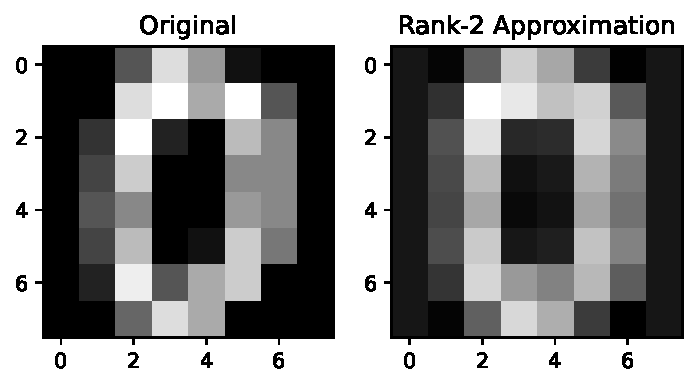
\includegraphics[keepaspectratio]{books/en-US/lab_files/figure-latex/cell-480-output-1.pdf}}

Even with just 2 singular values, the digit shape is recognizable.

\subsubsection{Try It Yourself}\label{try-it-yourself-182}

\begin{enumerate}
\def\labelenumi{\arabic{enumi}.}
\tightlist
\item
  Vary \(k\) in the image example (1, 2, 5, 10). How much detail do you
  keep?
\item
  Compare the approximation error \(\|A - A_k\|\) as \(k\) increases.
\item
  Apply low-rank approximation to random noisy data. Does it denoise?
\end{enumerate}

\subsubsection{The Takeaway}\label{the-takeaway-66}

\begin{itemize}
\tightlist
\item
  SVD gives the best possible low-rank approximation in terms of error.
\item
  By truncating singular values, you compress data while keeping its
  essential structure.
\item
  This is the backbone of image compression, recommender systems, and
  dimensionality reduction.
\end{itemize}

\subsection{85. Principal Component Analysis (Variance and
Directions)}\label{principal-component-analysis-variance-and-directions-1}

Principal Component Analysis (PCA) is one of the most important
applications of SVD. It finds the directions (principal components)
where data varies the most, and projects the data onto them to reduce
dimensionality while preserving as much information as possible.

Mathematically:

\begin{enumerate}
\def\labelenumi{\arabic{enumi}.}
\tightlist
\item
  Center the data (subtract the mean).
\item
  Compute covariance matrix \(C = \frac{1}{n} X^T X\).
\item
  Eigenvectors of \(C\) = principal directions.
\item
  Eigenvalues = variance explained.
\item
  Equivalently: PCA = SVD of centered data matrix.
\end{enumerate}

\subsubsection{Set Up Your Lab}\label{set-up-your-lab-84}

\begin{Shaded}
\begin{Highlighting}[]
\ImportTok{import}\NormalTok{ numpy }\ImportTok{as}\NormalTok{ np}
\ImportTok{import}\NormalTok{ matplotlib.pyplot }\ImportTok{as}\NormalTok{ plt}
\ImportTok{from}\NormalTok{ sklearn.datasets }\ImportTok{import}\NormalTok{ load\_digits}
\end{Highlighting}
\end{Shaded}

\subsubsection{Step-by-Step Code
Walkthrough}\label{step-by-step-code-walkthrough-84}

\begin{enumerate}
\def\labelenumi{\arabic{enumi}.}
\tightlist
\item
  Generate synthetic 2D data
\end{enumerate}

\begin{Shaded}
\begin{Highlighting}[]
\NormalTok{np.random.seed(}\DecValTok{0}\NormalTok{)}
\NormalTok{X }\OperatorTok{=}\NormalTok{ np.random.randn(}\DecValTok{200}\NormalTok{, }\DecValTok{2}\NormalTok{) }\OperatorTok{@}\NormalTok{ np.array([[}\DecValTok{3}\NormalTok{,}\DecValTok{1}\NormalTok{],[}\DecValTok{1}\NormalTok{,}\FloatTok{0.5}\NormalTok{]])  }\CommentTok{\# stretched cloud}

\NormalTok{plt.scatter(X[:,}\DecValTok{0}\NormalTok{], X[:,}\DecValTok{1}\NormalTok{], alpha}\OperatorTok{=}\FloatTok{0.3}\NormalTok{)}
\NormalTok{plt.title(}\StringTok{"Original data"}\NormalTok{)}
\NormalTok{plt.axis(}\StringTok{"equal"}\NormalTok{)}
\NormalTok{plt.show()}
\end{Highlighting}
\end{Shaded}

\pandocbounded{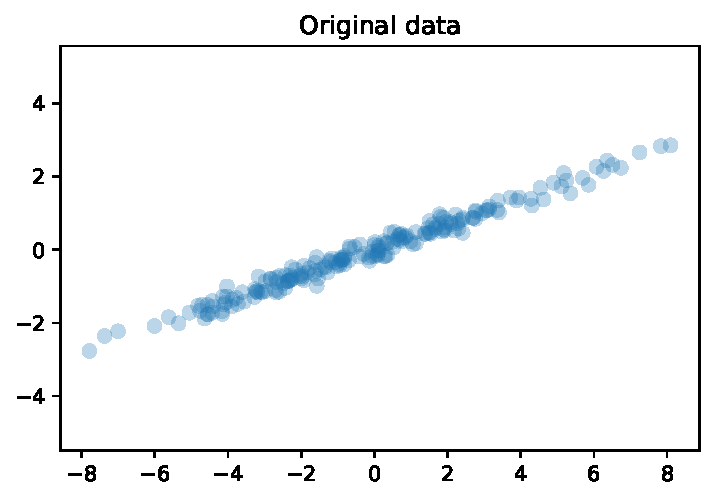
\includegraphics[keepaspectratio]{books/en-US/lab_files/figure-latex/cell-482-output-1.pdf}}

\begin{enumerate}
\def\labelenumi{\arabic{enumi}.}
\setcounter{enumi}{1}
\tightlist
\item
  Center the data
\end{enumerate}

\begin{Shaded}
\begin{Highlighting}[]
\NormalTok{X\_centered }\OperatorTok{=}\NormalTok{ X }\OperatorTok{{-}}\NormalTok{ X.mean(axis}\OperatorTok{=}\DecValTok{0}\NormalTok{)}
\end{Highlighting}
\end{Shaded}

\begin{enumerate}
\def\labelenumi{\arabic{enumi}.}
\setcounter{enumi}{2}
\tightlist
\item
  Compute SVD
\end{enumerate}

\begin{Shaded}
\begin{Highlighting}[]
\NormalTok{U, S, Vt }\OperatorTok{=}\NormalTok{ np.linalg.svd(X\_centered, full\_matrices}\OperatorTok{=}\VariableTok{False}\NormalTok{)}
\BuiltInTok{print}\NormalTok{(}\StringTok{"Principal directions (V):}\CharTok{\textbackslash{}n}\StringTok{"}\NormalTok{, Vt)}
\end{Highlighting}
\end{Shaded}

\begin{verbatim}
Principal directions (V):
 [[-0.94430098 -0.32908307]
 [ 0.32908307 -0.94430098]]
\end{verbatim}

Rows of \texttt{Vt} are the principal components.

\begin{enumerate}
\def\labelenumi{\arabic{enumi}.}
\setcounter{enumi}{3}
\tightlist
\item
  Project data onto first component
\end{enumerate}

\begin{Shaded}
\begin{Highlighting}[]
\NormalTok{X\_pca1 }\OperatorTok{=}\NormalTok{ X\_centered }\OperatorTok{@}\NormalTok{ Vt.T[:,}\DecValTok{0}\NormalTok{]}

\NormalTok{plt.scatter(X\_pca1, np.zeros\_like(X\_pca1), alpha}\OperatorTok{=}\FloatTok{0.3}\NormalTok{)}
\NormalTok{plt.title(}\StringTok{"Data projected on first principal component"}\NormalTok{)}
\NormalTok{plt.show()}
\end{Highlighting}
\end{Shaded}

\pandocbounded{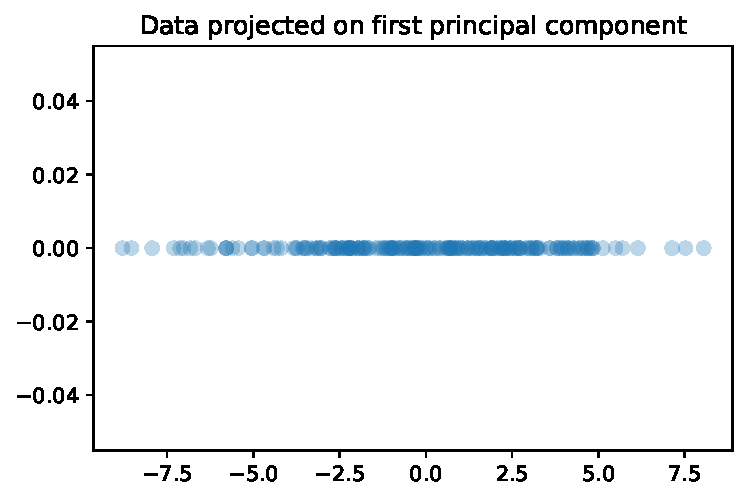
\includegraphics[keepaspectratio]{books/en-US/lab_files/figure-latex/cell-485-output-1.pdf}}

This collapses data into 1D, keeping the most variance.

\begin{enumerate}
\def\labelenumi{\arabic{enumi}.}
\setcounter{enumi}{4}
\tightlist
\item
  Visualize principal axes
\end{enumerate}

\begin{Shaded}
\begin{Highlighting}[]
\NormalTok{plt.scatter(X\_centered[:,}\DecValTok{0}\NormalTok{], X\_centered[:,}\DecValTok{1}\NormalTok{], alpha}\OperatorTok{=}\FloatTok{0.3}\NormalTok{)}
\ControlFlowTok{for}\NormalTok{ length, vector }\KeywordTok{in} \BuiltInTok{zip}\NormalTok{(S, Vt):}
\NormalTok{    plt.plot([}\DecValTok{0}\NormalTok{, vector[}\DecValTok{0}\NormalTok{]}\OperatorTok{*}\NormalTok{length], [}\DecValTok{0}\NormalTok{, vector[}\DecValTok{1}\NormalTok{]}\OperatorTok{*}\NormalTok{length], }\StringTok{\textquotesingle{}r{-}\textquotesingle{}}\NormalTok{, linewidth}\OperatorTok{=}\DecValTok{3}\NormalTok{)}
\NormalTok{plt.title(}\StringTok{"Principal components (directions of max variance)"}\NormalTok{)}
\NormalTok{plt.axis(}\StringTok{"equal"}\NormalTok{)}
\NormalTok{plt.show()}
\end{Highlighting}
\end{Shaded}

\pandocbounded{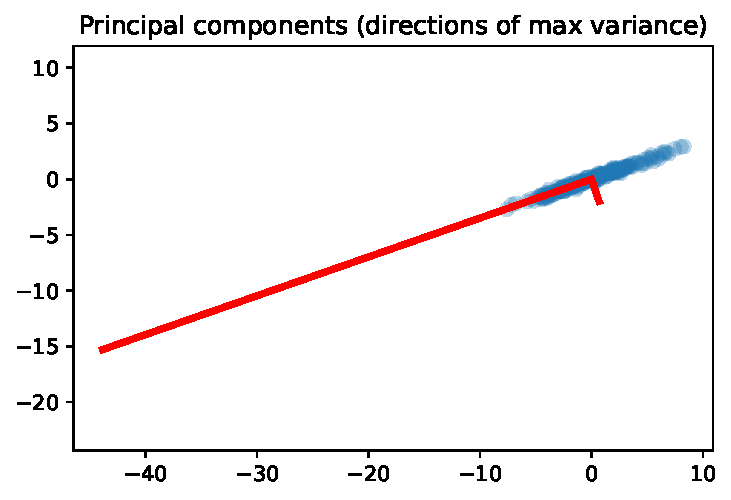
\includegraphics[keepaspectratio]{books/en-US/lab_files/figure-latex/cell-486-output-1.pdf}}

The red arrows show where the data spreads most.

\begin{enumerate}
\def\labelenumi{\arabic{enumi}.}
\setcounter{enumi}{5}
\tightlist
\item
  PCA on real data (digits)
\end{enumerate}

\begin{Shaded}
\begin{Highlighting}[]
\NormalTok{digits }\OperatorTok{=}\NormalTok{ load\_digits()}
\NormalTok{X }\OperatorTok{=}\NormalTok{ digits.data  }\CommentTok{\# 1797 samples, 64 features}
\NormalTok{X\_centered }\OperatorTok{=}\NormalTok{ X }\OperatorTok{{-}}\NormalTok{ X.mean(axis}\OperatorTok{=}\DecValTok{0}\NormalTok{)}

\NormalTok{U, S, Vt }\OperatorTok{=}\NormalTok{ np.linalg.svd(X\_centered, full\_matrices}\OperatorTok{=}\VariableTok{False}\NormalTok{)}

\NormalTok{explained\_variance }\OperatorTok{=}\NormalTok{ (S}\OperatorTok{**}\DecValTok{2}\NormalTok{) }\OperatorTok{/}\NormalTok{ np.}\BuiltInTok{sum}\NormalTok{(S}\OperatorTok{**}\DecValTok{2}\NormalTok{)}
\BuiltInTok{print}\NormalTok{(}\StringTok{"Explained variance ratio (first 5):"}\NormalTok{, explained\_variance[:}\DecValTok{5}\NormalTok{])}
\end{Highlighting}
\end{Shaded}

\begin{verbatim}
Explained variance ratio (first 5): [0.14890594 0.13618771 0.11794594 0.08409979 0.05782415]
\end{verbatim}

\subsubsection{Try It Yourself}\label{try-it-yourself-183}

\begin{enumerate}
\def\labelenumi{\arabic{enumi}.}
\tightlist
\item
  Reduce digits dataset to 2D using the top 2 components and plot. Do
  digit clusters separate?
\item
  Compare explained variance ratio for top 10 components.
\item
  Add noise to data and check if PCA filters it out when projecting to
  fewer dimensions.
\end{enumerate}

\subsubsection{The Takeaway}\label{the-takeaway-67}

\begin{itemize}
\tightlist
\item
  PCA finds directions of maximum variance using SVD.
\item
  By projecting onto top components, you compress data with minimal
  information loss.
\item
  PCA is the backbone of dimensionality reduction, visualization, and
  preprocessing in machine learning.
\end{itemize}

\subsection{86. Pseudoinverse (Moore--Penrose) and Solving Ill-Posed
Systems}\label{pseudoinverse-moorepenrose-and-solving-ill-posed-systems-1}

The Moore--Penrose pseudoinverse \(A^+\) generalizes the inverse of a
matrix. It allows solving systems \(Ax = b\) even when:

\begin{itemize}
\tightlist
\item
  \(A\) is not square, or
\item
  \(A\) is singular (non-invertible).
\end{itemize}

The solution given by the pseudoinverse is the least-squares solution
with minimum norm:

\[
x = A^+ b
\]

If \(A = U \Sigma V^T\), then:

\[
A^+ = V \Sigma^+ U^T
\]

where \(\Sigma^+\) is obtained by taking reciprocals of nonzero singular
values.

\subsubsection{Set Up Your Lab}\label{set-up-your-lab-85}

\begin{Shaded}
\begin{Highlighting}[]
\ImportTok{import}\NormalTok{ numpy }\ImportTok{as}\NormalTok{ np}
\end{Highlighting}
\end{Shaded}

\subsubsection{Step-by-Step Code
Walkthrough}\label{step-by-step-code-walkthrough-85}

\begin{enumerate}
\def\labelenumi{\arabic{enumi}.}
\tightlist
\item
  Solve an overdetermined system (more equations than unknowns)
\end{enumerate}

\begin{Shaded}
\begin{Highlighting}[]
\NormalTok{A }\OperatorTok{=}\NormalTok{ np.array([[}\DecValTok{1}\NormalTok{,}\DecValTok{1}\NormalTok{],}
\NormalTok{              [}\DecValTok{1}\NormalTok{,}\DecValTok{2}\NormalTok{],}
\NormalTok{              [}\DecValTok{1}\NormalTok{,}\DecValTok{3}\NormalTok{]])  }\CommentTok{\# 3x2 system}
\NormalTok{b }\OperatorTok{=}\NormalTok{ np.array([}\DecValTok{1}\NormalTok{,}\DecValTok{2}\NormalTok{,}\DecValTok{2}\NormalTok{])}

\NormalTok{x\_ls, }\OperatorTok{*}\NormalTok{\_ }\OperatorTok{=}\NormalTok{ np.linalg.lstsq(A, b, rcond}\OperatorTok{=}\VariableTok{None}\NormalTok{)}
\BuiltInTok{print}\NormalTok{(}\StringTok{"Least{-}squares solution:"}\NormalTok{, x\_ls)}
\end{Highlighting}
\end{Shaded}

\begin{verbatim}
Least-squares solution: [0.66666667 0.5       ]
\end{verbatim}

\begin{enumerate}
\def\labelenumi{\arabic{enumi}.}
\setcounter{enumi}{1}
\tightlist
\item
  Compute with pseudoinverse
\end{enumerate}

\begin{Shaded}
\begin{Highlighting}[]
\NormalTok{A\_pinv }\OperatorTok{=}\NormalTok{ np.linalg.pinv(A)}
\NormalTok{x\_pinv }\OperatorTok{=}\NormalTok{ A\_pinv }\OperatorTok{@}\NormalTok{ b}
\BuiltInTok{print}\NormalTok{(}\StringTok{"Pseudoinverse solution:"}\NormalTok{, x\_pinv)}
\end{Highlighting}
\end{Shaded}

\begin{verbatim}
Pseudoinverse solution: [0.66666667 0.5       ]
\end{verbatim}

Both match → pseudoinverse gives least-squares solution.

\begin{enumerate}
\def\labelenumi{\arabic{enumi}.}
\setcounter{enumi}{2}
\tightlist
\item
  Solve an underdetermined system (fewer equations than unknowns)
\end{enumerate}

\begin{Shaded}
\begin{Highlighting}[]
\NormalTok{A }\OperatorTok{=}\NormalTok{ np.array([[}\DecValTok{1}\NormalTok{,}\DecValTok{2}\NormalTok{,}\DecValTok{3}\NormalTok{]])  }\CommentTok{\# 1x3}
\NormalTok{b }\OperatorTok{=}\NormalTok{ np.array([}\DecValTok{1}\NormalTok{])}

\NormalTok{x\_pinv }\OperatorTok{=}\NormalTok{ np.linalg.pinv(A) }\OperatorTok{@}\NormalTok{ b}
\BuiltInTok{print}\NormalTok{(}\StringTok{"Minimum norm solution:"}\NormalTok{, x\_pinv)}
\end{Highlighting}
\end{Shaded}

\begin{verbatim}
Minimum norm solution: [0.07142857 0.14285714 0.21428571]
\end{verbatim}

Here, infinitely many solutions exist. The pseudoinverse picks the one
with smallest norm.

\begin{enumerate}
\def\labelenumi{\arabic{enumi}.}
\setcounter{enumi}{3}
\tightlist
\item
  Compare with singular matrix
\end{enumerate}

\begin{Shaded}
\begin{Highlighting}[]
\NormalTok{A }\OperatorTok{=}\NormalTok{ np.array([[}\DecValTok{1}\NormalTok{,}\DecValTok{2}\NormalTok{],}
\NormalTok{              [}\DecValTok{2}\NormalTok{,}\DecValTok{4}\NormalTok{]])  }\CommentTok{\# rank deficient}
\NormalTok{b }\OperatorTok{=}\NormalTok{ np.array([}\DecValTok{1}\NormalTok{,}\DecValTok{2}\NormalTok{])}

\NormalTok{x\_pinv }\OperatorTok{=}\NormalTok{ np.linalg.pinv(A) }\OperatorTok{@}\NormalTok{ b}
\BuiltInTok{print}\NormalTok{(}\StringTok{"Solution with pseudoinverse:"}\NormalTok{, x\_pinv)}
\end{Highlighting}
\end{Shaded}

\begin{verbatim}
Solution with pseudoinverse: [0.2 0.4]
\end{verbatim}

Even when \(A\) is singular, pseudoinverse provides a solution.

\begin{enumerate}
\def\labelenumi{\arabic{enumi}.}
\setcounter{enumi}{4}
\tightlist
\item
  Manual pseudoinverse via SVD
\end{enumerate}

\begin{Shaded}
\begin{Highlighting}[]
\NormalTok{A }\OperatorTok{=}\NormalTok{ np.array([[}\DecValTok{1}\NormalTok{,}\DecValTok{2}\NormalTok{],}
\NormalTok{              [}\DecValTok{3}\NormalTok{,}\DecValTok{4}\NormalTok{]])}
\NormalTok{U, S, Vt }\OperatorTok{=}\NormalTok{ np.linalg.svd(A)}
\NormalTok{S\_inv }\OperatorTok{=}\NormalTok{ np.zeros((Vt.shape[}\DecValTok{0}\NormalTok{], U.shape[}\DecValTok{0}\NormalTok{]))}
\ControlFlowTok{for}\NormalTok{ i }\KeywordTok{in} \BuiltInTok{range}\NormalTok{(}\BuiltInTok{len}\NormalTok{(S)):}
    \ControlFlowTok{if}\NormalTok{ S[i] }\OperatorTok{\textgreater{}} \FloatTok{1e{-}10}\NormalTok{:}
\NormalTok{        S\_inv[i,i] }\OperatorTok{=} \DecValTok{1}\OperatorTok{/}\NormalTok{S[i]}

\NormalTok{A\_pinv\_manual }\OperatorTok{=}\NormalTok{ Vt.T }\OperatorTok{@}\NormalTok{ S\_inv }\OperatorTok{@}\NormalTok{ U.T}
\BuiltInTok{print}\NormalTok{(}\StringTok{"Manual pseudoinverse:}\CharTok{\textbackslash{}n}\StringTok{"}\NormalTok{, A\_pinv\_manual)}
\BuiltInTok{print}\NormalTok{(}\StringTok{"NumPy pseudoinverse:}\CharTok{\textbackslash{}n}\StringTok{"}\NormalTok{, np.linalg.pinv(A))}
\end{Highlighting}
\end{Shaded}

\begin{verbatim}
Manual pseudoinverse:
 [[-2.   1. ]
 [ 1.5 -0.5]]
NumPy pseudoinverse:
 [[-2.   1. ]
 [ 1.5 -0.5]]
\end{verbatim}

They match.

\subsubsection{Try It Yourself}\label{try-it-yourself-184}

\begin{enumerate}
\def\labelenumi{\arabic{enumi}.}
\tightlist
\item
  Create an overdetermined system with noise and see how pseudoinverse
  smooths the solution.
\item
  Compare pseudoinverse with direct inverse (\texttt{np.linalg.inv}) on
  a square nonsingular matrix.
\item
  Zero out small singular values manually and see how solution changes.
\end{enumerate}

\subsubsection{The Takeaway}\label{the-takeaway-68}

\begin{itemize}
\tightlist
\item
  The pseudoinverse solves any linear system, square or not.
\item
  It provides the least-squares solution in overdetermined cases and the
  minimum-norm solution in underdetermined cases.
\item
  Built on SVD, it is a cornerstone of regression, optimization, and
  numerical methods.
\end{itemize}

\subsection{87. Conditioning and Sensitivity (How Errors
Amplify)}\label{conditioning-and-sensitivity-how-errors-amplify-1}

Conditioning tells us how sensitive a system is to small changes. For a
linear system \(Ax = b\):

\begin{itemize}
\tightlist
\item
  If \(A\) is well-conditioned, small changes in \(b\) or \(A\) → small
  changes in \(x\).
\item
  If \(A\) is ill-conditioned, tiny changes can cause huge swings in
  \(x\).
\end{itemize}

The condition number is defined as:

\[
\kappa(A) = \|A\| \cdot \|A^{-1}\|
\]

For SVD:

\[
\kappa(A) = \frac{\sigma_{\max}}{\sigma_{\min}}
\]

where \(\sigma_{\max}\) and \(\sigma_{\min}\) are the largest and
smallest singular values.

\begin{itemize}
\tightlist
\item
  Large \(\kappa(A)\) → unstable system.
\item
  Small \(\kappa(A)\) → stable system.
\end{itemize}

\subsubsection{Set Up Your Lab}\label{set-up-your-lab-86}

\begin{Shaded}
\begin{Highlighting}[]
\ImportTok{import}\NormalTok{ numpy }\ImportTok{as}\NormalTok{ np}
\end{Highlighting}
\end{Shaded}

\subsubsection{Step-by-Step Code
Walkthrough}\label{step-by-step-code-walkthrough-86}

\begin{enumerate}
\def\labelenumi{\arabic{enumi}.}
\tightlist
\item
  Well-conditioned system
\end{enumerate}

\begin{Shaded}
\begin{Highlighting}[]
\NormalTok{A }\OperatorTok{=}\NormalTok{ np.array([[}\DecValTok{2}\NormalTok{,}\DecValTok{0}\NormalTok{],}
\NormalTok{              [}\DecValTok{0}\NormalTok{,}\DecValTok{1}\NormalTok{]])}
\NormalTok{b }\OperatorTok{=}\NormalTok{ np.array([}\DecValTok{1}\NormalTok{,}\DecValTok{1}\NormalTok{])}

\NormalTok{x }\OperatorTok{=}\NormalTok{ np.linalg.solve(A, b)}
\NormalTok{cond }\OperatorTok{=}\NormalTok{ np.linalg.cond(A)}
\BuiltInTok{print}\NormalTok{(}\StringTok{"Solution:"}\NormalTok{, x)}
\BuiltInTok{print}\NormalTok{(}\StringTok{"Condition number:"}\NormalTok{, cond)}
\end{Highlighting}
\end{Shaded}

\begin{verbatim}
Solution: [0.5 1. ]
Condition number: 2.0
\end{verbatim}

Condition number = ratio of singular values → moderate size.

\begin{enumerate}
\def\labelenumi{\arabic{enumi}.}
\setcounter{enumi}{1}
\tightlist
\item
  Ill-conditioned system
\end{enumerate}

\begin{Shaded}
\begin{Highlighting}[]
\NormalTok{A }\OperatorTok{=}\NormalTok{ np.array([[}\DecValTok{1}\NormalTok{, }\FloatTok{1.0001}\NormalTok{],}
\NormalTok{              [}\DecValTok{1}\NormalTok{, }\FloatTok{1.0000}\NormalTok{]])}
\NormalTok{b }\OperatorTok{=}\NormalTok{ np.array([}\DecValTok{2}\NormalTok{,}\DecValTok{2}\NormalTok{])}

\NormalTok{x }\OperatorTok{=}\NormalTok{ np.linalg.lstsq(A, b, rcond}\OperatorTok{=}\VariableTok{None}\NormalTok{)[}\DecValTok{0}\NormalTok{]}
\NormalTok{cond }\OperatorTok{=}\NormalTok{ np.linalg.cond(A)}
\BuiltInTok{print}\NormalTok{(}\StringTok{"Solution:"}\NormalTok{, x)}
\BuiltInTok{print}\NormalTok{(}\StringTok{"Condition number:"}\NormalTok{, cond)}
\end{Highlighting}
\end{Shaded}

\begin{verbatim}
Solution: [ 2.00000000e+00 -5.73526099e-13]
Condition number: 40002.000075017124
\end{verbatim}

Condition number is very large → instability.

\begin{enumerate}
\def\labelenumi{\arabic{enumi}.}
\setcounter{enumi}{2}
\tightlist
\item
  Perturb the right-hand side
\end{enumerate}

\begin{Shaded}
\begin{Highlighting}[]
\NormalTok{b2 }\OperatorTok{=}\NormalTok{ np.array([}\DecValTok{2}\NormalTok{, }\FloatTok{2.001}\NormalTok{])  }\CommentTok{\# tiny change}
\NormalTok{x2 }\OperatorTok{=}\NormalTok{ np.linalg.lstsq(A, b2, rcond}\OperatorTok{=}\VariableTok{None}\NormalTok{)[}\DecValTok{0}\NormalTok{]}
\BuiltInTok{print}\NormalTok{(}\StringTok{"Solution after tiny change:"}\NormalTok{, x2)}
\end{Highlighting}
\end{Shaded}

\begin{verbatim}
Solution after tiny change: [ 12.001 -10.   ]
\end{verbatim}

The solution changes drastically → shows sensitivity.

\begin{enumerate}
\def\labelenumi{\arabic{enumi}.}
\setcounter{enumi}{3}
\tightlist
\item
  Relation to singular values
\end{enumerate}

\begin{Shaded}
\begin{Highlighting}[]
\NormalTok{U, S, Vt }\OperatorTok{=}\NormalTok{ np.linalg.svd(A)}
\BuiltInTok{print}\NormalTok{(}\StringTok{"Singular values:"}\NormalTok{, S)}
\BuiltInTok{print}\NormalTok{(}\StringTok{"Condition number (SVD):"}\NormalTok{, S[}\DecValTok{0}\NormalTok{]}\OperatorTok{/}\NormalTok{S[}\OperatorTok{{-}}\DecValTok{1}\NormalTok{])}
\end{Highlighting}
\end{Shaded}

\begin{verbatim}
Singular values: [2.000050e+00 4.999875e-05]
Condition number (SVD): 40002.00007501713
\end{verbatim}

\begin{enumerate}
\def\labelenumi{\arabic{enumi}.}
\setcounter{enumi}{4}
\tightlist
\item
  Scaling experiment
\end{enumerate}

\begin{Shaded}
\begin{Highlighting}[]
\ControlFlowTok{for}\NormalTok{ scale }\KeywordTok{in}\NormalTok{ [}\DecValTok{1}\NormalTok{,}\FloatTok{1e{-}2}\NormalTok{,}\FloatTok{1e{-}4}\NormalTok{,}\FloatTok{1e{-}6}\NormalTok{]:}
\NormalTok{    A }\OperatorTok{=}\NormalTok{ np.array([[}\DecValTok{1}\NormalTok{,}\DecValTok{0}\NormalTok{],[}\DecValTok{0}\NormalTok{,scale]])}
    \BuiltInTok{print}\NormalTok{(}\SpecialStringTok{f"Scale=}\SpecialCharTok{\{}\NormalTok{scale}\SpecialCharTok{\}}\SpecialStringTok{, condition number=}\SpecialCharTok{\{}\NormalTok{np}\SpecialCharTok{.}\NormalTok{linalg}\SpecialCharTok{.}\NormalTok{cond(A)}\SpecialCharTok{\}}\SpecialStringTok{"}\NormalTok{)}
\end{Highlighting}
\end{Shaded}

\begin{verbatim}
Scale=1, condition number=1.0
Scale=0.01, condition number=100.0
Scale=0.0001, condition number=10000.0
Scale=1e-06, condition number=1000000.0
\end{verbatim}

As scale shrinks, condition number explodes.

\subsubsection{Try It Yourself}\label{try-it-yourself-185}

\begin{enumerate}
\def\labelenumi{\arabic{enumi}.}
\tightlist
\item
  Generate random matrices and compute their condition numbers. Which
  are stable?
\item
  Compare condition numbers of Hilbert matrices (notoriously
  ill-conditioned).
\item
  Explore how rounding errors grow with high condition numbers.
\end{enumerate}

\subsubsection{The Takeaway}\label{the-takeaway-69}

\begin{itemize}
\tightlist
\item
  Condition number = measure of problem sensitivity.
\item
  \(\kappa(A) = \sigma_{\max}/\sigma_{\min}\).
\item
  Ill-conditioned problems amplify errors and are numerically unstable →
  why scaling, regularization, and good formulations matter.
\end{itemize}

\subsection{88. Matrix Norms and Singular Values (Measuring Size
Properly)}\label{matrix-norms-and-singular-values-measuring-size-properly-1}

Matrix norms measure the size or strength of a matrix. They extend the
idea of vector length to matrices. Norms are crucial for analyzing
stability, error growth, and performance of algorithms.

Some important norms:

\begin{itemize}
\tightlist
\item
  Frobenius norm:
\end{itemize}

\[
\|A\|_F = \sqrt{\sum_{i,j} |a_{ij}|^2}
\]

Equivalent to treating the matrix as a big vector.

\begin{itemize}
\tightlist
\item
  Spectral norm (operator 2-norm):
\end{itemize}

\[
\|A\|_2 = \sigma_{\max}
\]

The largest singular value - tells how much \(A\) can stretch a vector.

\begin{itemize}
\tightlist
\item
  1-norm: maximum absolute column sum.
\item
  ∞-norm: maximum absolute row sum.
\end{itemize}

\subsubsection{Set Up Your Lab}\label{set-up-your-lab-87}

\begin{Shaded}
\begin{Highlighting}[]
\ImportTok{import}\NormalTok{ numpy }\ImportTok{as}\NormalTok{ np}
\end{Highlighting}
\end{Shaded}

\subsubsection{Step-by-Step Code
Walkthrough}\label{step-by-step-code-walkthrough-87}

\begin{enumerate}
\def\labelenumi{\arabic{enumi}.}
\tightlist
\item
  Build a test matrix
\end{enumerate}

\begin{Shaded}
\begin{Highlighting}[]
\NormalTok{A }\OperatorTok{=}\NormalTok{ np.array([[}\DecValTok{1}\NormalTok{, }\OperatorTok{{-}}\DecValTok{2}\NormalTok{, }\DecValTok{3}\NormalTok{],}
\NormalTok{              [}\DecValTok{0}\NormalTok{,  }\DecValTok{4}\NormalTok{, }\DecValTok{5}\NormalTok{],}
\NormalTok{              [}\OperatorTok{{-}}\DecValTok{1}\NormalTok{, }\DecValTok{2}\NormalTok{, }\DecValTok{1}\NormalTok{]])}
\end{Highlighting}
\end{Shaded}

\begin{enumerate}
\def\labelenumi{\arabic{enumi}.}
\setcounter{enumi}{1}
\tightlist
\item
  Compute different norms
\end{enumerate}

\begin{Shaded}
\begin{Highlighting}[]
\NormalTok{fro }\OperatorTok{=}\NormalTok{ np.linalg.norm(A, }\StringTok{\textquotesingle{}fro\textquotesingle{}}\NormalTok{)}
\NormalTok{spec }\OperatorTok{=}\NormalTok{ np.linalg.norm(A, }\DecValTok{2}\NormalTok{)}
\NormalTok{one\_norm }\OperatorTok{=}\NormalTok{ np.linalg.norm(A, }\DecValTok{1}\NormalTok{)}
\NormalTok{inf\_norm }\OperatorTok{=}\NormalTok{ np.linalg.norm(A, np.inf)}

\BuiltInTok{print}\NormalTok{(}\StringTok{"Frobenius norm:"}\NormalTok{, fro)}
\BuiltInTok{print}\NormalTok{(}\StringTok{"Spectral norm:"}\NormalTok{, spec)}
\BuiltInTok{print}\NormalTok{(}\StringTok{"1{-}norm:"}\NormalTok{, one\_norm)}
\BuiltInTok{print}\NormalTok{(}\StringTok{"Infinity norm:"}\NormalTok{, inf\_norm)}
\end{Highlighting}
\end{Shaded}

\begin{verbatim}
Frobenius norm: 7.810249675906654
Spectral norm: 6.813953458914004
1-norm: 9.0
Infinity norm: 9.0
\end{verbatim}

\begin{enumerate}
\def\labelenumi{\arabic{enumi}.}
\setcounter{enumi}{2}
\tightlist
\item
  Compare spectral norm with largest singular value
\end{enumerate}

\begin{Shaded}
\begin{Highlighting}[]
\NormalTok{U, S, Vt }\OperatorTok{=}\NormalTok{ np.linalg.svd(A)}
\BuiltInTok{print}\NormalTok{(}\StringTok{"Largest singular value:"}\NormalTok{, S[}\DecValTok{0}\NormalTok{])}
\BuiltInTok{print}\NormalTok{(}\StringTok{"Spectral norm:"}\NormalTok{, spec)}
\end{Highlighting}
\end{Shaded}

\begin{verbatim}
Largest singular value: 6.813953458914004
Spectral norm: 6.813953458914004
\end{verbatim}

They match → spectral norm = largest singular value.

\begin{enumerate}
\def\labelenumi{\arabic{enumi}.}
\setcounter{enumi}{3}
\tightlist
\item
  Frobenius norm from singular values
\end{enumerate}

\[
\|A\|_F = \sqrt{\sigma_1^2 + \sigma_2^2 + \dots}
\]

\begin{Shaded}
\begin{Highlighting}[]
\NormalTok{fro\_from\_svd }\OperatorTok{=}\NormalTok{ np.sqrt(np.}\BuiltInTok{sum}\NormalTok{(S}\OperatorTok{**}\DecValTok{2}\NormalTok{))}
\BuiltInTok{print}\NormalTok{(}\StringTok{"Frobenius norm (from SVD):"}\NormalTok{, fro\_from\_svd)}
\end{Highlighting}
\end{Shaded}

\begin{verbatim}
Frobenius norm (from SVD): 7.810249675906654
\end{verbatim}

\begin{enumerate}
\def\labelenumi{\arabic{enumi}.}
\setcounter{enumi}{4}
\tightlist
\item
  Stretching effect demonstration
\end{enumerate}

Pick a random vector and see how much it grows:

\begin{Shaded}
\begin{Highlighting}[]
\NormalTok{x }\OperatorTok{=}\NormalTok{ np.random.randn(}\DecValTok{3}\NormalTok{)}
\NormalTok{stretch }\OperatorTok{=}\NormalTok{ np.linalg.norm(A }\OperatorTok{@}\NormalTok{ x) }\OperatorTok{/}\NormalTok{ np.linalg.norm(x)}
\BuiltInTok{print}\NormalTok{(}\StringTok{"Stretch factor:"}\NormalTok{, stretch)}
\BuiltInTok{print}\NormalTok{(}\StringTok{"Spectral norm (max possible stretch):"}\NormalTok{, spec)}
\end{Highlighting}
\end{Shaded}

\begin{verbatim}
Stretch factor: 2.7537463268177698
Spectral norm (max possible stretch): 6.813953458914004
\end{verbatim}

The stretch ≤ spectral norm, always.

\subsubsection{Try It Yourself}\label{try-it-yourself-186}

\begin{enumerate}
\def\labelenumi{\arabic{enumi}.}
\tightlist
\item
  Compare norms for diagonal matrices - do they match the largest
  diagonal entry?
\item
  Generate random matrices and see how norms differ.
\item
  Compute Frobenius vs spectral norm for a rank-1 matrix.
\end{enumerate}

\subsubsection{The Takeaway}\label{the-takeaway-70}

\begin{itemize}
\tightlist
\item
  Frobenius norm = overall energy of the matrix.
\item
  Spectral norm = maximum stretching power (largest singular value).
\item
  Other norms (1-norm, ∞-norm) capture row/column dominance.
\item
  Singular values unify all these views of ``matrix size.''
\end{itemize}

\subsection{89. Regularization (Ridge/Tikhonov to Tame
Instability)}\label{regularization-ridgetikhonov-to-tame-instability-1}

When solving \(Ax = b\), if \(A\) is ill-conditioned (large condition
number), small errors in data can cause huge errors in the solution.
Regularization stabilizes the problem by adding a penalty term that
discourages extreme solutions.

The most common form: ridge regression (a.k.a. Tikhonov regularization):

\[
x_\lambda = \arg\min_x \|Ax - b\|^2 + \lambda \|x\|^2
\]

Closed form:

\[
x_\lambda = (A^T A + \lambda I)^{-1} A^T b
\]

Here \(\lambda > 0\) controls the amount of regularization:

\begin{itemize}
\tightlist
\item
  Small \(\lambda\): solution close to least-squares.
\item
  Large \(\lambda\): smaller coefficients, more stability.
\end{itemize}

\subsubsection{Set Up Your Lab}\label{set-up-your-lab-88}

\begin{Shaded}
\begin{Highlighting}[]
\ImportTok{import}\NormalTok{ numpy }\ImportTok{as}\NormalTok{ np}
\ImportTok{import}\NormalTok{ matplotlib.pyplot }\ImportTok{as}\NormalTok{ plt}
\end{Highlighting}
\end{Shaded}

\subsubsection{Step-by-Step Code
Walkthrough}\label{step-by-step-code-walkthrough-88}

\begin{enumerate}
\def\labelenumi{\arabic{enumi}.}
\tightlist
\item
  Build an ill-conditioned system
\end{enumerate}

\begin{Shaded}
\begin{Highlighting}[]
\NormalTok{A }\OperatorTok{=}\NormalTok{ np.array([[}\DecValTok{1}\NormalTok{, }\FloatTok{1.001}\NormalTok{],}
\NormalTok{              [}\DecValTok{1}\NormalTok{, }\FloatTok{0.999}\NormalTok{]])}
\NormalTok{b }\OperatorTok{=}\NormalTok{ np.array([}\DecValTok{2}\NormalTok{, }\DecValTok{2}\NormalTok{])}
\end{Highlighting}
\end{Shaded}

\begin{enumerate}
\def\labelenumi{\arabic{enumi}.}
\setcounter{enumi}{1}
\tightlist
\item
  Solve without regularization
\end{enumerate}

\begin{Shaded}
\begin{Highlighting}[]
\NormalTok{x\_ls, }\OperatorTok{*}\NormalTok{\_ }\OperatorTok{=}\NormalTok{ np.linalg.lstsq(A, b, rcond}\OperatorTok{=}\VariableTok{None}\NormalTok{)}
\BuiltInTok{print}\NormalTok{(}\StringTok{"Least squares solution:"}\NormalTok{, x\_ls)}
\end{Highlighting}
\end{Shaded}

\begin{verbatim}
Least squares solution: [ 2.00000000e+00 -2.84186735e-14]
\end{verbatim}

The result may be unstable.

\begin{enumerate}
\def\labelenumi{\arabic{enumi}.}
\setcounter{enumi}{2}
\tightlist
\item
  Apply ridge regularization
\end{enumerate}

\begin{Shaded}
\begin{Highlighting}[]
\NormalTok{lam }\OperatorTok{=} \FloatTok{0.1}
\NormalTok{x\_ridge }\OperatorTok{=}\NormalTok{ np.linalg.inv(A.T }\OperatorTok{@}\NormalTok{ A }\OperatorTok{+}\NormalTok{ lam}\OperatorTok{*}\NormalTok{np.eye(}\DecValTok{2}\NormalTok{)) }\OperatorTok{@}\NormalTok{ A.T }\OperatorTok{@}\NormalTok{ b}
\BuiltInTok{print}\NormalTok{(}\StringTok{"Ridge solution (λ=0.1):"}\NormalTok{, x\_ridge)}
\end{Highlighting}
\end{Shaded}

\begin{verbatim}
Ridge solution (λ=0.1): [0.97561927 0.97559976]
\end{verbatim}

\begin{enumerate}
\def\labelenumi{\arabic{enumi}.}
\setcounter{enumi}{3}
\tightlist
\item
  Compare effect of different λ
\end{enumerate}

\begin{Shaded}
\begin{Highlighting}[]
\NormalTok{lambdas }\OperatorTok{=}\NormalTok{ np.logspace(}\OperatorTok{{-}}\DecValTok{4}\NormalTok{, }\DecValTok{2}\NormalTok{, }\DecValTok{20}\NormalTok{)}
\NormalTok{solutions }\OperatorTok{=}\NormalTok{ []}
\ControlFlowTok{for}\NormalTok{ lam }\KeywordTok{in}\NormalTok{ lambdas:}
\NormalTok{    x\_reg }\OperatorTok{=}\NormalTok{ np.linalg.inv(A.T }\OperatorTok{@}\NormalTok{ A }\OperatorTok{+}\NormalTok{ lam}\OperatorTok{*}\NormalTok{np.eye(}\DecValTok{2}\NormalTok{)) }\OperatorTok{@}\NormalTok{ A.T }\OperatorTok{@}\NormalTok{ b}
\NormalTok{    solutions.append(np.linalg.norm(x\_reg))}

\NormalTok{plt.semilogx(lambdas, solutions, }\StringTok{\textquotesingle{}o{-}\textquotesingle{}}\NormalTok{)}
\NormalTok{plt.xlabel(}\StringTok{"λ (regularization strength)"}\NormalTok{)}
\NormalTok{plt.ylabel(}\StringTok{"Solution norm"}\NormalTok{)}
\NormalTok{plt.title(}\StringTok{"Effect of ridge regularization"}\NormalTok{)}
\NormalTok{plt.show()}
\end{Highlighting}
\end{Shaded}

\pandocbounded{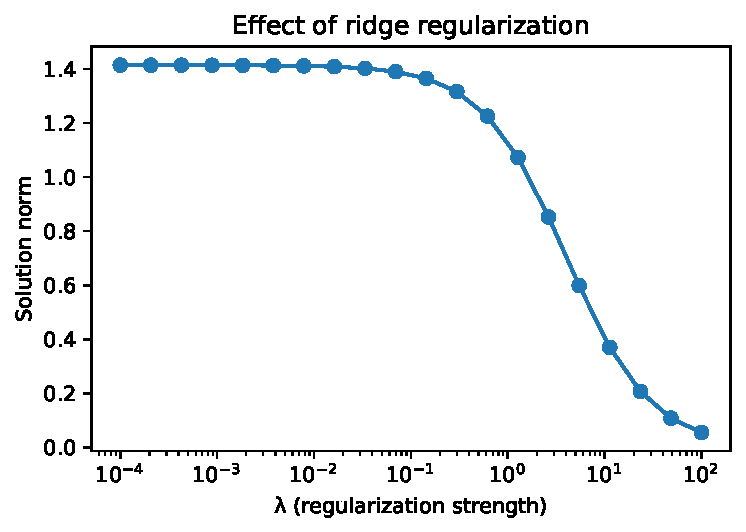
\includegraphics[keepaspectratio]{books/en-US/lab_files/figure-latex/cell-510-output-1.pdf}}

As \(\lambda\) increases, the solution becomes smaller and more stable.

\begin{enumerate}
\def\labelenumi{\arabic{enumi}.}
\setcounter{enumi}{4}
\tightlist
\item
  Connection to SVD
\end{enumerate}

If \(A = U \Sigma V^T\):

\[
x_\lambda = \sum_i \frac{\sigma_i}{\sigma_i^2 + \lambda} (u_i^T b) v_i
\]

Small singular values (causing instability) get damped by
\(\frac{\sigma_i}{\sigma_i^2 + \lambda}\).

\subsubsection{Try It Yourself}\label{try-it-yourself-187}

\begin{enumerate}
\def\labelenumi{\arabic{enumi}.}
\tightlist
\item
  Experiment with larger and smaller \(\lambda\). What happens to the
  solution?
\item
  Add random noise to \(b\). Compare least-squares vs ridge stability.
\item
  Plot how each coefficient changes with λ.
\end{enumerate}

\subsubsection{The Takeaway}\label{the-takeaway-71}

\begin{itemize}
\tightlist
\item
  Regularization controls instability in ill-conditioned problems.
\item
  Ridge regression balances fit vs.~stability using λ.
\item
  In SVD terms, regularization damps small singular values that cause
  wild solutions.
\end{itemize}

\subsection{90. Rank-Revealing QR and Practical Diagnostics (What Rank
Really
Is)}\label{rank-revealing-qr-and-practical-diagnostics-what-rank-really-is-1}

In practice, we often need to determine the numerical rank of a matrix -
not just the theoretical rank, but how many directions carry meaningful
information beyond round-off errors or noise. A useful tool for this is
the Rank-Revealing QR (RRQR) factorization.

For a matrix \(A\):

\[
A P = Q R
\]

\begin{itemize}
\tightlist
\item
  \(Q\): orthogonal matrix
\item
  \(R\): upper triangular matrix
\item
  \(P\): column permutation matrix
\end{itemize}

By reordering columns smartly, the diagonal of \(R\) reveals which
directions are significant.

\subsubsection{Set Up Your Lab}\label{set-up-your-lab-89}

\begin{Shaded}
\begin{Highlighting}[]
\ImportTok{import}\NormalTok{ numpy }\ImportTok{as}\NormalTok{ np}
\ImportTok{from}\NormalTok{ scipy.linalg }\ImportTok{import}\NormalTok{ qr}
\end{Highlighting}
\end{Shaded}

\subsubsection{Step-by-Step Code
Walkthrough}\label{step-by-step-code-walkthrough-89}

\begin{enumerate}
\def\labelenumi{\arabic{enumi}.}
\tightlist
\item
  Build a nearly rank-deficient matrix
\end{enumerate}

\begin{Shaded}
\begin{Highlighting}[]
\NormalTok{A }\OperatorTok{=}\NormalTok{ np.array([[}\DecValTok{1}\NormalTok{, }\DecValTok{2}\NormalTok{, }\DecValTok{3}\NormalTok{],}
\NormalTok{              [}\DecValTok{2}\NormalTok{, }\FloatTok{4.001}\NormalTok{, }\DecValTok{6}\NormalTok{],}
\NormalTok{              [}\DecValTok{3}\NormalTok{, }\DecValTok{6}\NormalTok{, }\FloatTok{9.001}\NormalTok{]])}
\BuiltInTok{print}\NormalTok{(}\StringTok{"Rank (theoretical):"}\NormalTok{, np.linalg.matrix\_rank(A))}
\end{Highlighting}
\end{Shaded}

\begin{verbatim}
Rank (theoretical): 3
\end{verbatim}

This matrix is almost rank 2 but with small perturbations.

\begin{enumerate}
\def\labelenumi{\arabic{enumi}.}
\setcounter{enumi}{1}
\tightlist
\item
  QR with column pivoting
\end{enumerate}

\begin{Shaded}
\begin{Highlighting}[]
\NormalTok{Q, R, P }\OperatorTok{=}\NormalTok{ qr(A, pivoting}\OperatorTok{=}\VariableTok{True}\NormalTok{)}
\BuiltInTok{print}\NormalTok{(}\StringTok{"R:}\CharTok{\textbackslash{}n}\StringTok{"}\NormalTok{, R)}
\BuiltInTok{print}\NormalTok{(}\StringTok{"Column permutation:"}\NormalTok{, P)}
\end{Highlighting}
\end{Shaded}

\begin{verbatim}
R:
 [[-1.12257740e+01 -7.48384925e+00 -3.74165738e+00]
 [ 0.00000000e+00 -1.20185042e-03 -1.84886859e-04]
 [ 0.00000000e+00  0.00000000e+00 -7.41196374e-05]]
Column permutation: [2 1 0]
\end{verbatim}

The diagonal entries of \(R\) decrease rapidly → numerical rank is
determined where they become tiny.

\begin{enumerate}
\def\labelenumi{\arabic{enumi}.}
\setcounter{enumi}{2}
\tightlist
\item
  Compare with SVD
\end{enumerate}

\begin{Shaded}
\begin{Highlighting}[]
\NormalTok{U, S, Vt }\OperatorTok{=}\NormalTok{ np.linalg.svd(A)}
\BuiltInTok{print}\NormalTok{(}\StringTok{"Singular values:"}\NormalTok{, S)}
\end{Highlighting}
\end{Shaded}

\begin{verbatim}
Singular values: [1.40009286e+01 1.00000000e-03 7.14238341e-05]
\end{verbatim}

The singular values tell the same story: one is very small → effective
rank ≈ 2.

\begin{enumerate}
\def\labelenumi{\arabic{enumi}.}
\setcounter{enumi}{3}
\tightlist
\item
  Thresholding for rank
\end{enumerate}

\begin{Shaded}
\begin{Highlighting}[]
\NormalTok{tol }\OperatorTok{=} \FloatTok{1e{-}3}
\NormalTok{rank\_est }\OperatorTok{=}\NormalTok{ np.}\BuiltInTok{sum}\NormalTok{(S }\OperatorTok{\textgreater{}}\NormalTok{ tol)}
\BuiltInTok{print}\NormalTok{(}\StringTok{"Estimated rank:"}\NormalTok{, rank\_est)}
\end{Highlighting}
\end{Shaded}

\begin{verbatim}
Estimated rank: 2
\end{verbatim}

\begin{enumerate}
\def\labelenumi{\arabic{enumi}.}
\setcounter{enumi}{4}
\tightlist
\item
  Diagnostics on a noisy matrix
\end{enumerate}

\begin{Shaded}
\begin{Highlighting}[]
\NormalTok{np.random.seed(}\DecValTok{0}\NormalTok{)}
\NormalTok{B }\OperatorTok{=}\NormalTok{ np.random.randn(}\DecValTok{50}\NormalTok{, }\DecValTok{10}\NormalTok{) }\OperatorTok{@}\NormalTok{ np.random.randn(}\DecValTok{10}\NormalTok{, }\DecValTok{10}\NormalTok{)  }\CommentTok{\# rank ≤ 10}
\NormalTok{B[:, }\OperatorTok{{-}}\DecValTok{1}\NormalTok{] }\OperatorTok{+=} \FloatTok{1e{-}6} \OperatorTok{*}\NormalTok{ np.random.randn(}\DecValTok{50}\NormalTok{)  }\CommentTok{\# tiny noise}

\NormalTok{U, S, Vt }\OperatorTok{=}\NormalTok{ np.linalg.svd(B)}
\NormalTok{plt.semilogy(S, }\StringTok{\textquotesingle{}o{-}\textquotesingle{}}\NormalTok{)}
\NormalTok{plt.title(}\StringTok{"Singular values (log scale)"}\NormalTok{)}
\NormalTok{plt.xlabel(}\StringTok{"Index"}\NormalTok{)}
\NormalTok{plt.ylabel(}\StringTok{"Value"}\NormalTok{)}
\NormalTok{plt.show()}
\end{Highlighting}
\end{Shaded}

\pandocbounded{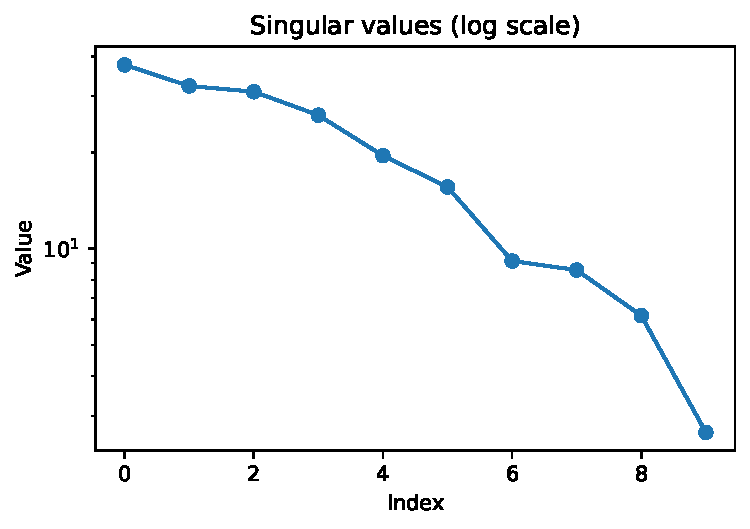
\includegraphics[keepaspectratio]{books/en-US/lab_files/figure-latex/cell-516-output-1.pdf}}

The drop in singular values shows effective rank.

\subsubsection{Try It Yourself}\label{try-it-yourself-188}

\begin{enumerate}
\def\labelenumi{\arabic{enumi}.}
\tightlist
\item
  Change the perturbation in \(A\) from 0.001 to 0.000001. Does the
  numerical rank change?
\item
  Test QR with pivoting on random rectangular matrices.
\item
  Compare rank estimates from QR vs SVD for large noisy matrices.
\end{enumerate}

\subsubsection{The Takeaway}\label{the-takeaway-72}

\begin{itemize}
\tightlist
\item
  Rank-revealing QR is a practical tool to detect effective rank in
  real-world data.
\item
  SVD gives the most precise picture (singular values), but QR with
  pivoting is faster.
\item
  Understanding numerical rank is crucial for diagnostics, stability,
  and model complexity control.
\end{itemize}

\section{Chapter 10. Applications and
computation}\label{chapter-10.-applications-and-computation-2}

\subsection{91. 2D/3D Geometry Pipelines (Cameras, Rotations, and
Transforms)}\label{d3d-geometry-pipelines-cameras-rotations-and-transforms-1}

Linear algebra powers the geometry pipelines in computer graphics and
robotics.

\begin{itemize}
\tightlist
\item
  2D transforms: rotation, scaling, translation.
\item
  3D transforms: same ideas, but with an extra dimension.
\item
  Homogeneous coordinates let us unify all transforms (even
  translations) into matrix multiplications.
\end{itemize}

\subsubsection{Set Up Your Lab}\label{set-up-your-lab-90}

\begin{Shaded}
\begin{Highlighting}[]
\ImportTok{import}\NormalTok{ numpy }\ImportTok{as}\NormalTok{ np}
\ImportTok{import}\NormalTok{ matplotlib.pyplot }\ImportTok{as}\NormalTok{ plt}
\end{Highlighting}
\end{Shaded}

\subsubsection{Step-by-Step Code
Walkthrough}\label{step-by-step-code-walkthrough-90}

\begin{enumerate}
\def\labelenumi{\arabic{enumi}.}
\tightlist
\item
  Rotation in 2D
\end{enumerate}

\[
R(\theta) = 
\begin{bmatrix}
\cos\theta & -\sin\theta \\
\sin\theta & \cos\theta
\end{bmatrix}
\]

\begin{Shaded}
\begin{Highlighting}[]
\NormalTok{theta }\OperatorTok{=}\NormalTok{ np.pi}\OperatorTok{/}\DecValTok{4}  \CommentTok{\# 45 degrees}
\NormalTok{R }\OperatorTok{=}\NormalTok{ np.array([[np.cos(theta), }\OperatorTok{{-}}\NormalTok{np.sin(theta)],}
\NormalTok{              [np.sin(theta),  np.cos(theta)]])}

\NormalTok{point }\OperatorTok{=}\NormalTok{ np.array([}\DecValTok{1}\NormalTok{, }\DecValTok{0}\NormalTok{])}
\NormalTok{rotated }\OperatorTok{=}\NormalTok{ R }\OperatorTok{@}\NormalTok{ point}

\BuiltInTok{print}\NormalTok{(}\StringTok{"Original:"}\NormalTok{, point)}
\BuiltInTok{print}\NormalTok{(}\StringTok{"Rotated:"}\NormalTok{, rotated)}
\end{Highlighting}
\end{Shaded}

\begin{verbatim}
Original: [1 0]
Rotated: [0.70710678 0.70710678]
\end{verbatim}

\begin{enumerate}
\def\labelenumi{\arabic{enumi}.}
\setcounter{enumi}{1}
\tightlist
\item
  Translation using homogeneous coordinates
\end{enumerate}

In 2D:

\[
T(dx, dy) =
\begin{bmatrix}
1 & 0 & dx \\
0 & 1 & dy \\
0 & 0 & 1
\end{bmatrix}
\]

\begin{Shaded}
\begin{Highlighting}[]
\NormalTok{T }\OperatorTok{=}\NormalTok{ np.array([[}\DecValTok{1}\NormalTok{,}\DecValTok{0}\NormalTok{,}\DecValTok{2}\NormalTok{],}
\NormalTok{              [}\DecValTok{0}\NormalTok{,}\DecValTok{1}\NormalTok{,}\DecValTok{1}\NormalTok{],}
\NormalTok{              [}\DecValTok{0}\NormalTok{,}\DecValTok{0}\NormalTok{,}\DecValTok{1}\NormalTok{]])}

\NormalTok{p\_h }\OperatorTok{=}\NormalTok{ np.array([}\DecValTok{1}\NormalTok{,}\DecValTok{1}\NormalTok{,}\DecValTok{1}\NormalTok{])  }\CommentTok{\# homogeneous (x=1,y=1)}
\NormalTok{translated }\OperatorTok{=}\NormalTok{ T }\OperatorTok{@}\NormalTok{ p\_h}
\BuiltInTok{print}\NormalTok{(}\StringTok{"Translated point:"}\NormalTok{, translated)}
\end{Highlighting}
\end{Shaded}

\begin{verbatim}
Translated point: [3 2 1]
\end{verbatim}

\begin{enumerate}
\def\labelenumi{\arabic{enumi}.}
\setcounter{enumi}{2}
\tightlist
\item
  Combine rotation + translation
\end{enumerate}

Transformations compose by multiplying matrices.

\begin{Shaded}
\begin{Highlighting}[]
\NormalTok{M }\OperatorTok{=}\NormalTok{ T }\OperatorTok{@}\NormalTok{ np.block([[R, np.zeros((}\DecValTok{2}\NormalTok{,}\DecValTok{1}\NormalTok{))],}
\NormalTok{                  [np.zeros((}\DecValTok{1}\NormalTok{,}\DecValTok{2}\NormalTok{)), }\DecValTok{1}\NormalTok{]])}
\NormalTok{combined }\OperatorTok{=}\NormalTok{ M }\OperatorTok{@}\NormalTok{ p\_h}
\BuiltInTok{print}\NormalTok{(}\StringTok{"Combined transform (rotation+translation):"}\NormalTok{, combined)}
\end{Highlighting}
\end{Shaded}

\begin{verbatim}
Combined transform (rotation+translation): [2.         2.41421356 1.        ]
\end{verbatim}

\begin{enumerate}
\def\labelenumi{\arabic{enumi}.}
\setcounter{enumi}{3}
\tightlist
\item
  3D rotation (around z-axis)
\end{enumerate}

\[
R_z(\theta) =
\begin{bmatrix}
\cos\theta & -\sin\theta & 0 \\
\sin\theta &  \cos\theta & 0 \\
0          & 0           & 1
\end{bmatrix}
\]

\begin{Shaded}
\begin{Highlighting}[]
\NormalTok{theta }\OperatorTok{=}\NormalTok{ np.pi}\OperatorTok{/}\DecValTok{3}
\NormalTok{Rz }\OperatorTok{=}\NormalTok{ np.array([[np.cos(theta), }\OperatorTok{{-}}\NormalTok{np.sin(theta), }\DecValTok{0}\NormalTok{],}
\NormalTok{               [np.sin(theta),  np.cos(theta), }\DecValTok{0}\NormalTok{],}
\NormalTok{               [}\DecValTok{0}\NormalTok{,              }\DecValTok{0}\NormalTok{,             }\DecValTok{1}\NormalTok{]])}

\NormalTok{point3d }\OperatorTok{=}\NormalTok{ np.array([}\DecValTok{1}\NormalTok{,}\DecValTok{0}\NormalTok{,}\DecValTok{0}\NormalTok{])}
\NormalTok{rotated3d }\OperatorTok{=}\NormalTok{ Rz }\OperatorTok{@}\NormalTok{ point3d}
\BuiltInTok{print}\NormalTok{(}\StringTok{"3D rotated point:"}\NormalTok{, rotated3d)}
\end{Highlighting}
\end{Shaded}

\begin{verbatim}
3D rotated point: [0.5       0.8660254 0.       ]
\end{verbatim}

\begin{enumerate}
\def\labelenumi{\arabic{enumi}.}
\setcounter{enumi}{4}
\tightlist
\item
  Camera projection (3D → 2D)
\end{enumerate}

Simple pinhole model:

\[
\begin{bmatrix}
x' \\
y'
\end{bmatrix}
=
\begin{bmatrix}
f \cdot x / z \\
f \cdot y / z
\end{bmatrix}
\]

\begin{Shaded}
\begin{Highlighting}[]
\NormalTok{f }\OperatorTok{=} \FloatTok{1.0}  \CommentTok{\# focal length}
\NormalTok{P }\OperatorTok{=}\NormalTok{ np.array([[f,}\DecValTok{0}\NormalTok{,}\DecValTok{0}\NormalTok{],}
\NormalTok{              [}\DecValTok{0}\NormalTok{,f,}\DecValTok{0}\NormalTok{],}
\NormalTok{              [}\DecValTok{0}\NormalTok{,}\DecValTok{0}\NormalTok{,}\DecValTok{1}\NormalTok{]])  }\CommentTok{\# projection matrix}

\NormalTok{point3d }\OperatorTok{=}\NormalTok{ np.array([}\DecValTok{2}\NormalTok{,}\DecValTok{3}\NormalTok{,}\DecValTok{5}\NormalTok{])}
\NormalTok{p\_proj }\OperatorTok{=}\NormalTok{ P }\OperatorTok{@}\NormalTok{ point3d}
\NormalTok{p\_proj }\OperatorTok{=}\NormalTok{ p\_proj[:}\DecValTok{2}\NormalTok{] }\OperatorTok{/}\NormalTok{ p\_proj[}\DecValTok{2}\NormalTok{]  }\CommentTok{\# divide by z}
\BuiltInTok{print}\NormalTok{(}\StringTok{"Projected 2D point:"}\NormalTok{, p\_proj)}
\end{Highlighting}
\end{Shaded}

\begin{verbatim}
Projected 2D point: [0.4 0.6]
\end{verbatim}

\subsubsection{Try It Yourself}\label{try-it-yourself-189}

\begin{enumerate}
\def\labelenumi{\arabic{enumi}.}
\tightlist
\item
  Rotate a square in 2D, then translate it. Plot before/after.
\item
  Rotate a 3D point cloud around x, y, and z axes.
\item
  Project a cube into 2D using the pinhole camera model.
\end{enumerate}

\subsubsection{The Takeaway}\label{the-takeaway-73}

\begin{itemize}
\tightlist
\item
  Geometry pipelines = sequences of linear transforms.
\item
  Homogeneous coordinates unify rotation, scaling, and translation.
\item
  Camera projection links 3D world to 2D images - a cornerstone of
  graphics and vision.
\end{itemize}

\subsection{92. Computer Graphics and Robotics (Homogeneous Tricks in
Action)}\label{computer-graphics-and-robotics-homogeneous-tricks-in-action-1}

Computer graphics and robotics both rely on homogeneous coordinates to
unify rotations, translations, scalings, and projections into a single
framework. With \(4 \times 4\) matrices in 3D, entire transformation
pipelines can be built as matrix products.

\subsubsection{Set Up Your Lab}\label{set-up-your-lab-91}

\begin{Shaded}
\begin{Highlighting}[]
\ImportTok{import}\NormalTok{ numpy }\ImportTok{as}\NormalTok{ np}
\ImportTok{import}\NormalTok{ matplotlib.pyplot }\ImportTok{as}\NormalTok{ plt}
\end{Highlighting}
\end{Shaded}

\subsubsection{Step-by-Step Code
Walkthrough}\label{step-by-step-code-walkthrough-91}

\begin{enumerate}
\def\labelenumi{\arabic{enumi}.}
\tightlist
\item
  Homogeneous representation of a point
\end{enumerate}

In 3D:

\[
(x, y, z) \mapsto (x, y, z, 1)
\]

\begin{Shaded}
\begin{Highlighting}[]
\NormalTok{p }\OperatorTok{=}\NormalTok{ np.array([}\DecValTok{1}\NormalTok{,}\DecValTok{2}\NormalTok{,}\DecValTok{3}\NormalTok{,}\DecValTok{1}\NormalTok{])  }\CommentTok{\# homogeneous point}
\end{Highlighting}
\end{Shaded}

\begin{enumerate}
\def\labelenumi{\arabic{enumi}.}
\setcounter{enumi}{1}
\tightlist
\item
  Define translation, rotation, and scaling matrices
\end{enumerate}

\begin{itemize}
\tightlist
\item
  Translation by \((dx,dy,dz)\):
\end{itemize}

\begin{Shaded}
\begin{Highlighting}[]
\NormalTok{T }\OperatorTok{=}\NormalTok{ np.array([[}\DecValTok{1}\NormalTok{,}\DecValTok{0}\NormalTok{,}\DecValTok{0}\NormalTok{,}\DecValTok{2}\NormalTok{],}
\NormalTok{              [}\DecValTok{0}\NormalTok{,}\DecValTok{1}\NormalTok{,}\DecValTok{0}\NormalTok{,}\DecValTok{1}\NormalTok{],}
\NormalTok{              [}\DecValTok{0}\NormalTok{,}\DecValTok{0}\NormalTok{,}\DecValTok{1}\NormalTok{,}\DecValTok{3}\NormalTok{],}
\NormalTok{              [}\DecValTok{0}\NormalTok{,}\DecValTok{0}\NormalTok{,}\DecValTok{0}\NormalTok{,}\DecValTok{1}\NormalTok{]])}
\end{Highlighting}
\end{Shaded}

\begin{itemize}
\tightlist
\item
  Scaling by factors \((sx, sy, sz)\):
\end{itemize}

\begin{Shaded}
\begin{Highlighting}[]
\NormalTok{S }\OperatorTok{=}\NormalTok{ np.diag([}\DecValTok{2}\NormalTok{, }\FloatTok{0.5}\NormalTok{, }\FloatTok{1.5}\NormalTok{, }\DecValTok{1}\NormalTok{])}
\end{Highlighting}
\end{Shaded}

\begin{itemize}
\tightlist
\item
  Rotation about z-axis (\(\theta = 90^\circ\)):
\end{itemize}

\begin{Shaded}
\begin{Highlighting}[]
\NormalTok{theta }\OperatorTok{=}\NormalTok{ np.pi}\OperatorTok{/}\DecValTok{2}
\NormalTok{Rz }\OperatorTok{=}\NormalTok{ np.array([[np.cos(theta), }\OperatorTok{{-}}\NormalTok{np.sin(theta), }\DecValTok{0}\NormalTok{, }\DecValTok{0}\NormalTok{],}
\NormalTok{               [np.sin(theta),  np.cos(theta), }\DecValTok{0}\NormalTok{, }\DecValTok{0}\NormalTok{],}
\NormalTok{               [}\DecValTok{0}\NormalTok{,              }\DecValTok{0}\NormalTok{,             }\DecValTok{1}\NormalTok{, }\DecValTok{0}\NormalTok{],}
\NormalTok{               [}\DecValTok{0}\NormalTok{,              }\DecValTok{0}\NormalTok{,             }\DecValTok{0}\NormalTok{, }\DecValTok{1}\NormalTok{]])}
\end{Highlighting}
\end{Shaded}

\begin{enumerate}
\def\labelenumi{\arabic{enumi}.}
\setcounter{enumi}{2}
\tightlist
\item
  Combine transforms into a pipeline
\end{enumerate}

\begin{Shaded}
\begin{Highlighting}[]
\NormalTok{M }\OperatorTok{=}\NormalTok{ T }\OperatorTok{@}\NormalTok{ Rz }\OperatorTok{@}\NormalTok{ S  }\CommentTok{\# first scale, then rotate, then translate}
\NormalTok{p\_transformed }\OperatorTok{=}\NormalTok{ M }\OperatorTok{@}\NormalTok{ p}
\BuiltInTok{print}\NormalTok{(}\StringTok{"Transformed point:"}\NormalTok{, p\_transformed)}
\end{Highlighting}
\end{Shaded}

\begin{verbatim}
Transformed point: [1.  3.  7.5 1. ]
\end{verbatim}

\begin{enumerate}
\def\labelenumi{\arabic{enumi}.}
\setcounter{enumi}{3}
\tightlist
\item
  Robotics: forward kinematics of a 2-link arm
\end{enumerate}

Each joint is a rotation + translation.

\begin{Shaded}
\begin{Highlighting}[]
\KeywordTok{def}\NormalTok{ link(theta, length):}
    \ControlFlowTok{return}\NormalTok{ np.array([[np.cos(theta), }\OperatorTok{{-}}\NormalTok{np.sin(theta), }\DecValTok{0}\NormalTok{, length}\OperatorTok{*}\NormalTok{np.cos(theta)],}
\NormalTok{                     [np.sin(theta),  np.cos(theta), }\DecValTok{0}\NormalTok{, length}\OperatorTok{*}\NormalTok{np.sin(theta)],}
\NormalTok{                     [}\DecValTok{0}\NormalTok{,              }\DecValTok{0}\NormalTok{,             }\DecValTok{1}\NormalTok{, }\DecValTok{0}\NormalTok{],}
\NormalTok{                     [}\DecValTok{0}\NormalTok{,              }\DecValTok{0}\NormalTok{,             }\DecValTok{0}\NormalTok{, }\DecValTok{1}\NormalTok{]])}

\NormalTok{theta1, theta2 }\OperatorTok{=}\NormalTok{ np.pi}\OperatorTok{/}\DecValTok{4}\NormalTok{, np.pi}\OperatorTok{/}\DecValTok{6}
\NormalTok{L1, L2 }\OperatorTok{=} \DecValTok{2}\NormalTok{, }\FloatTok{1.5}

\NormalTok{M1 }\OperatorTok{=}\NormalTok{ link(theta1, L1)}
\NormalTok{M2 }\OperatorTok{=}\NormalTok{ link(theta2, L2)}

\NormalTok{end\_effector }\OperatorTok{=}\NormalTok{ M1 }\OperatorTok{@}\NormalTok{ M2 }\OperatorTok{@}\NormalTok{ np.array([}\DecValTok{0}\NormalTok{,}\DecValTok{0}\NormalTok{,}\DecValTok{0}\NormalTok{,}\DecValTok{1}\NormalTok{])}
\BuiltInTok{print}\NormalTok{(}\StringTok{"End effector position:"}\NormalTok{, end\_effector[:}\DecValTok{3}\NormalTok{])}
\end{Highlighting}
\end{Shaded}

\begin{verbatim}
End effector position: [1.80244213 2.8631023  0.        ]
\end{verbatim}

\begin{enumerate}
\def\labelenumi{\arabic{enumi}.}
\setcounter{enumi}{4}
\tightlist
\item
  Graphics: simple 3D camera projection
\end{enumerate}

\begin{Shaded}
\begin{Highlighting}[]
\NormalTok{f }\OperatorTok{=} \FloatTok{2.0}
\NormalTok{P }\OperatorTok{=}\NormalTok{ np.array([[f,}\DecValTok{0}\NormalTok{,}\DecValTok{0}\NormalTok{,}\DecValTok{0}\NormalTok{],}
\NormalTok{              [}\DecValTok{0}\NormalTok{,f,}\DecValTok{0}\NormalTok{,}\DecValTok{0}\NormalTok{],}
\NormalTok{              [}\DecValTok{0}\NormalTok{,}\DecValTok{0}\NormalTok{,}\DecValTok{1}\NormalTok{,}\DecValTok{0}\NormalTok{]])}

\NormalTok{cube }\OperatorTok{=}\NormalTok{ np.array([[x,y,z,}\DecValTok{1}\NormalTok{] }\ControlFlowTok{for}\NormalTok{ x }\KeywordTok{in}\NormalTok{ [}\DecValTok{0}\NormalTok{,}\DecValTok{1}\NormalTok{] }\ControlFlowTok{for}\NormalTok{ y }\KeywordTok{in}\NormalTok{ [}\DecValTok{0}\NormalTok{,}\DecValTok{1}\NormalTok{] }\ControlFlowTok{for}\NormalTok{ z }\KeywordTok{in}\NormalTok{ [}\DecValTok{0}\NormalTok{,}\DecValTok{1}\NormalTok{]])}
\NormalTok{proj }\OperatorTok{=}\NormalTok{ (P }\OperatorTok{@}\NormalTok{ cube.T).T}
\NormalTok{proj2d }\OperatorTok{=}\NormalTok{ proj[:,:}\DecValTok{2}\NormalTok{] }\OperatorTok{/}\NormalTok{ proj[:,}\DecValTok{2}\NormalTok{:}\DecValTok{3}\NormalTok{]}

\NormalTok{plt.scatter(proj2d[:,}\DecValTok{0}\NormalTok{], proj2d[:,}\DecValTok{1}\NormalTok{])}
\NormalTok{plt.title(}\StringTok{"Projected cube"}\NormalTok{)}
\NormalTok{plt.show()}
\end{Highlighting}
\end{Shaded}

\begin{verbatim}
/var/folders/_g/lq_pglm508df70x751kkxrl80000gp/T/ipykernel_31637/2038614107.py:8: RuntimeWarning: divide by zero encountered in divide
  proj2d = proj[:,:2] / proj[:,2:3]
/var/folders/_g/lq_pglm508df70x751kkxrl80000gp/T/ipykernel_31637/2038614107.py:8: RuntimeWarning: invalid value encountered in divide
  proj2d = proj[:,:2] / proj[:,2:3]
\end{verbatim}

\pandocbounded{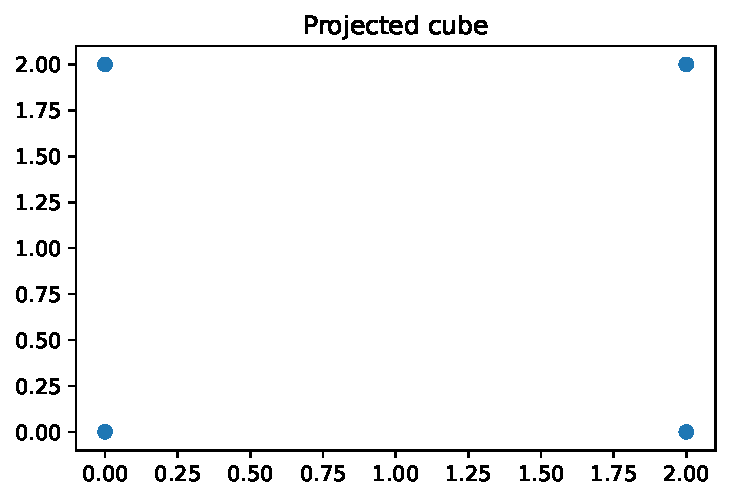
\includegraphics[keepaspectratio]{books/en-US/lab_files/figure-latex/cell-530-output-2.pdf}}

\subsubsection{Try It Yourself}\label{try-it-yourself-190}

\begin{enumerate}
\def\labelenumi{\arabic{enumi}.}
\tightlist
\item
  Change order of transforms (\texttt{Rz\ @\ S\ @\ T}). How does the
  result differ?
\item
  Add a third joint to the robotic arm and compute new end-effector
  position.
\item
  Project the cube with different focal lengths \(f\).
\end{enumerate}

\subsubsection{The Takeaway}\label{the-takeaway-74}

\begin{itemize}
\tightlist
\item
  Homogeneous coordinates unify all transformations.
\item
  Robotics uses this framework for forward kinematics.
\item
  Graphics uses it for camera and projection pipelines.
\item
  Both fields rely on the same linear algebra tricks - just applied
  differently.
\end{itemize}

\subsection{93. Graphs, Adjacency, and Laplacians (Networks via
Matrices)}\label{graphs-adjacency-and-laplacians-networks-via-matrices-1}

Graphs can be studied with linear algebra by encoding them into
matrices. Two of the most important:

\begin{itemize}
\item
  Adjacency matrix \(A\):

  \[
  A_{ij} = 
  \begin{cases} 
  1 & \text{if edge between i and j exists} \\
  0 & \text{otherwise}
  \end{cases}
  \]
\item
  Graph Laplacian \(L\):

  \[
  L = D - A
  \]

  where \(D\) is the degree matrix (\$D\_\{ii\} = \$ number of neighbors
  of node \(i\)).
\end{itemize}

These matrices let us analyze connectivity, diffusion, and clustering.

\subsubsection{Set Up Your Lab}\label{set-up-your-lab-92}

\begin{Shaded}
\begin{Highlighting}[]
\ImportTok{import}\NormalTok{ numpy }\ImportTok{as}\NormalTok{ np}
\ImportTok{import}\NormalTok{ networkx }\ImportTok{as}\NormalTok{ nx}
\ImportTok{import}\NormalTok{ matplotlib.pyplot }\ImportTok{as}\NormalTok{ plt}
\end{Highlighting}
\end{Shaded}

\subsubsection{Step-by-Step Code
Walkthrough}\label{step-by-step-code-walkthrough-92}

\begin{enumerate}
\def\labelenumi{\arabic{enumi}.}
\tightlist
\item
  Build a simple graph
\end{enumerate}

\begin{Shaded}
\begin{Highlighting}[]
\NormalTok{G }\OperatorTok{=}\NormalTok{ nx.Graph()}
\NormalTok{G.add\_edges\_from([(}\DecValTok{0}\NormalTok{,}\DecValTok{1}\NormalTok{), (}\DecValTok{1}\NormalTok{,}\DecValTok{2}\NormalTok{), (}\DecValTok{2}\NormalTok{,}\DecValTok{3}\NormalTok{), (}\DecValTok{3}\NormalTok{,}\DecValTok{0}\NormalTok{), (}\DecValTok{0}\NormalTok{,}\DecValTok{2}\NormalTok{)])  }\CommentTok{\# square with diagonal}

\NormalTok{nx.draw(G, with\_labels}\OperatorTok{=}\VariableTok{True}\NormalTok{, node\_color}\OperatorTok{=}\StringTok{"lightblue"}\NormalTok{, node\_size}\OperatorTok{=}\DecValTok{800}\NormalTok{)}
\NormalTok{plt.show()}
\end{Highlighting}
\end{Shaded}

\pandocbounded{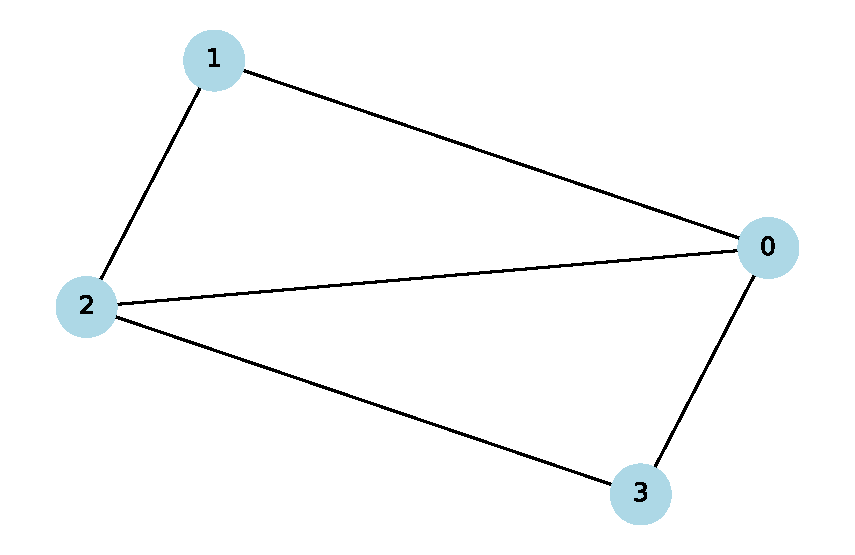
\includegraphics[keepaspectratio]{books/en-US/lab_files/figure-latex/cell-532-output-1.pdf}}

\begin{enumerate}
\def\labelenumi{\arabic{enumi}.}
\setcounter{enumi}{1}
\tightlist
\item
  Adjacency matrix
\end{enumerate}

\begin{Shaded}
\begin{Highlighting}[]
\NormalTok{A }\OperatorTok{=}\NormalTok{ nx.to\_numpy\_array(G)}
\BuiltInTok{print}\NormalTok{(}\StringTok{"Adjacency matrix:}\CharTok{\textbackslash{}n}\StringTok{"}\NormalTok{, A)}
\end{Highlighting}
\end{Shaded}

\begin{verbatim}
Adjacency matrix:
 [[0. 1. 1. 1.]
 [1. 0. 1. 0.]
 [1. 1. 0. 1.]
 [1. 0. 1. 0.]]
\end{verbatim}

\begin{enumerate}
\def\labelenumi{\arabic{enumi}.}
\setcounter{enumi}{2}
\tightlist
\item
  Degree and Laplacian matrices
\end{enumerate}

\begin{Shaded}
\begin{Highlighting}[]
\NormalTok{D }\OperatorTok{=}\NormalTok{ np.diag(A.}\BuiltInTok{sum}\NormalTok{(axis}\OperatorTok{=}\DecValTok{1}\NormalTok{))}
\NormalTok{L }\OperatorTok{=}\NormalTok{ D }\OperatorTok{{-}}\NormalTok{ A}
\BuiltInTok{print}\NormalTok{(}\StringTok{"Degree matrix:}\CharTok{\textbackslash{}n}\StringTok{"}\NormalTok{, D)}
\BuiltInTok{print}\NormalTok{(}\StringTok{"Graph Laplacian:}\CharTok{\textbackslash{}n}\StringTok{"}\NormalTok{, L)}
\end{Highlighting}
\end{Shaded}

\begin{verbatim}
Degree matrix:
 [[3. 0. 0. 0.]
 [0. 2. 0. 0.]
 [0. 0. 3. 0.]
 [0. 0. 0. 2.]]
Graph Laplacian:
 [[ 3. -1. -1. -1.]
 [-1.  2. -1.  0.]
 [-1. -1.  3. -1.]
 [-1.  0. -1.  2.]]
\end{verbatim}

\begin{enumerate}
\def\labelenumi{\arabic{enumi}.}
\setcounter{enumi}{3}
\tightlist
\item
  Eigenvalues of Laplacian (connectivity check)
\end{enumerate}

\begin{Shaded}
\begin{Highlighting}[]
\NormalTok{eigvals, eigvecs }\OperatorTok{=}\NormalTok{ np.linalg.eigh(L)}
\BuiltInTok{print}\NormalTok{(}\StringTok{"Laplacian eigenvalues:"}\NormalTok{, eigvals)}
\end{Highlighting}
\end{Shaded}

\begin{verbatim}
Laplacian eigenvalues: [1.11022302e-16 2.00000000e+00 4.00000000e+00 4.00000000e+00]
\end{verbatim}

\begin{itemize}
\tightlist
\item
  The number of zero eigenvalues = number of connected components.
\end{itemize}

\begin{enumerate}
\def\labelenumi{\arabic{enumi}.}
\setcounter{enumi}{4}
\tightlist
\item
  Spectral embedding (clustering)
\end{enumerate}

Use Laplacian eigenvectors to embed nodes in low dimensions.

\begin{Shaded}
\begin{Highlighting}[]
\NormalTok{coords }\OperatorTok{=}\NormalTok{ eigvecs[:,}\DecValTok{1}\NormalTok{:}\DecValTok{3}\NormalTok{]  }\CommentTok{\# skip the trivial first eigenvector}
\NormalTok{plt.scatter(coords[:,}\DecValTok{0}\NormalTok{], coords[:,}\DecValTok{1}\NormalTok{], c}\OperatorTok{=}\BuiltInTok{range}\NormalTok{(}\BuiltInTok{len}\NormalTok{(coords)), cmap}\OperatorTok{=}\StringTok{"tab10"}\NormalTok{, s}\OperatorTok{=}\DecValTok{200}\NormalTok{)}
\ControlFlowTok{for}\NormalTok{ i, (x,y) }\KeywordTok{in} \BuiltInTok{enumerate}\NormalTok{(coords):}
\NormalTok{    plt.text(x, y, }\BuiltInTok{str}\NormalTok{(i), fontsize}\OperatorTok{=}\DecValTok{12}\NormalTok{, ha}\OperatorTok{=}\StringTok{"center"}\NormalTok{, va}\OperatorTok{=}\StringTok{"center"}\NormalTok{, color}\OperatorTok{=}\StringTok{"white"}\NormalTok{)}
\NormalTok{plt.title(}\StringTok{"Spectral embedding of graph"}\NormalTok{)}
\NormalTok{plt.show()}
\end{Highlighting}
\end{Shaded}

\pandocbounded{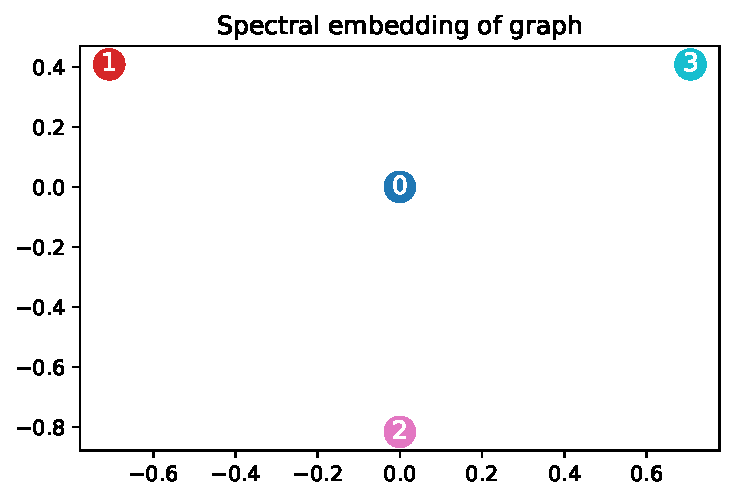
\includegraphics[keepaspectratio]{books/en-US/lab_files/figure-latex/cell-536-output-1.pdf}}

\subsubsection{Try It Yourself}\label{try-it-yourself-191}

\begin{enumerate}
\def\labelenumi{\arabic{enumi}.}
\tightlist
\item
  Remove one edge from the graph and see how Laplacian eigenvalues
  change.
\item
  Add a disconnected node - does an extra zero eigenvalue appear?
\item
  Try a random graph and compare adjacency vs Laplacian spectra.
\end{enumerate}

\subsubsection{The Takeaway}\label{the-takeaway-75}

\begin{itemize}
\tightlist
\item
  Adjacency matrices describe direct graph structure.
\item
  Laplacians capture connectivity and diffusion.
\item
  Eigenvalues of \(L\) reveal graph properties like connectedness and
  clustering - bridging networks with linear algebra.
\end{itemize}

\subsection{94. Data Preprocessing as Linear Ops (Centering, Whitening,
Scaling)}\label{data-preprocessing-as-linear-ops-centering-whitening-scaling}

Many machine learning and data analysis workflows begin with
preprocessing, and linear algebra provides the tools.

\begin{itemize}
\tightlist
\item
  Centering: subtract the mean → move data to origin.
\item
  Scaling: divide by standard deviation → normalize feature ranges.
\item
  Whitening: decorrelate features → make covariance matrix the identity.
\end{itemize}

Each step can be written as a matrix operation.

\subsubsection{Set Up Your Lab}\label{set-up-your-lab-93}

\begin{Shaded}
\begin{Highlighting}[]
\ImportTok{import}\NormalTok{ numpy }\ImportTok{as}\NormalTok{ np}
\ImportTok{import}\NormalTok{ matplotlib.pyplot }\ImportTok{as}\NormalTok{ plt}
\end{Highlighting}
\end{Shaded}

\subsubsection{Step-by-Step Code
Walkthrough}\label{step-by-step-code-walkthrough-93}

\begin{enumerate}
\def\labelenumi{\arabic{enumi}.}
\tightlist
\item
  Generate correlated data
\end{enumerate}

\begin{Shaded}
\begin{Highlighting}[]
\NormalTok{np.random.seed(}\DecValTok{0}\NormalTok{)}
\NormalTok{X }\OperatorTok{=}\NormalTok{ np.random.randn(}\DecValTok{200}\NormalTok{, }\DecValTok{2}\NormalTok{) }\OperatorTok{@}\NormalTok{ np.array([[}\DecValTok{3}\NormalTok{,}\DecValTok{1}\NormalTok{],[}\DecValTok{1}\NormalTok{,}\FloatTok{0.5}\NormalTok{]])}
\NormalTok{plt.scatter(X[:,}\DecValTok{0}\NormalTok{], X[:,}\DecValTok{1}\NormalTok{], alpha}\OperatorTok{=}\FloatTok{0.4}\NormalTok{)}
\NormalTok{plt.title(}\StringTok{"Original correlated data"}\NormalTok{)}
\NormalTok{plt.axis(}\StringTok{"equal"}\NormalTok{)}
\NormalTok{plt.show()}
\end{Highlighting}
\end{Shaded}

\pandocbounded{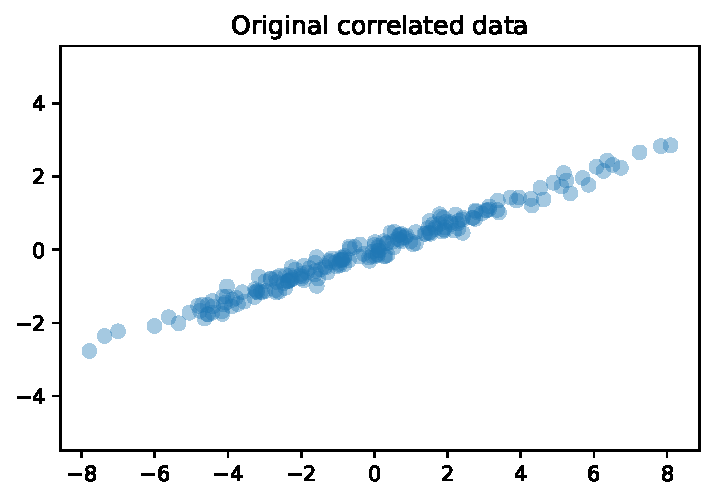
\includegraphics[keepaspectratio]{books/en-US/lab_files/figure-latex/cell-538-output-1.pdf}}

\begin{enumerate}
\def\labelenumi{\arabic{enumi}.}
\setcounter{enumi}{1}
\tightlist
\item
  Centering (subtract mean)
\end{enumerate}

\begin{Shaded}
\begin{Highlighting}[]
\NormalTok{X\_centered }\OperatorTok{=}\NormalTok{ X }\OperatorTok{{-}}\NormalTok{ X.mean(axis}\OperatorTok{=}\DecValTok{0}\NormalTok{)}
\BuiltInTok{print}\NormalTok{(}\StringTok{"Mean after centering:"}\NormalTok{, X\_centered.mean(axis}\OperatorTok{=}\DecValTok{0}\NormalTok{))}
\end{Highlighting}
\end{Shaded}

\begin{verbatim}
Mean after centering: [ 8.88178420e-18 -1.22124533e-17]
\end{verbatim}

\begin{enumerate}
\def\labelenumi{\arabic{enumi}.}
\setcounter{enumi}{2}
\tightlist
\item
  Scaling (normalize features)
\end{enumerate}

\begin{Shaded}
\begin{Highlighting}[]
\NormalTok{X\_scaled }\OperatorTok{=}\NormalTok{ X\_centered }\OperatorTok{/}\NormalTok{ X\_centered.std(axis}\OperatorTok{=}\DecValTok{0}\NormalTok{)}
\BuiltInTok{print}\NormalTok{(}\StringTok{"Std after scaling:"}\NormalTok{, X\_scaled.std(axis}\OperatorTok{=}\DecValTok{0}\NormalTok{))}
\end{Highlighting}
\end{Shaded}

\begin{verbatim}
Std after scaling: [1. 1.]
\end{verbatim}

\begin{enumerate}
\def\labelenumi{\arabic{enumi}.}
\setcounter{enumi}{3}
\tightlist
\item
  Whitening via eigen-decomposition
\end{enumerate}

Covariance of centered data:

\begin{Shaded}
\begin{Highlighting}[]
\NormalTok{C }\OperatorTok{=}\NormalTok{ np.cov(X\_centered.T)}
\NormalTok{eigvals, eigvecs }\OperatorTok{=}\NormalTok{ np.linalg.eigh(C)}

\NormalTok{W }\OperatorTok{=}\NormalTok{ eigvecs }\OperatorTok{@}\NormalTok{ np.diag(}\DecValTok{1}\OperatorTok{/}\NormalTok{np.sqrt(eigvals)) }\OperatorTok{@}\NormalTok{ eigvecs.T}
\NormalTok{X\_white }\OperatorTok{=}\NormalTok{ X\_centered }\OperatorTok{@}\NormalTok{ W}
\end{Highlighting}
\end{Shaded}

Check covariance:

\begin{Shaded}
\begin{Highlighting}[]
\BuiltInTok{print}\NormalTok{(}\StringTok{"Whitened covariance:}\CharTok{\textbackslash{}n}\StringTok{"}\NormalTok{, np.cov(X\_white.T))}
\end{Highlighting}
\end{Shaded}

\begin{verbatim}
Whitened covariance:
 [[1.00000000e+00 2.54402864e-15]
 [2.54402864e-15 1.00000000e+00]]
\end{verbatim}

\begin{enumerate}
\def\labelenumi{\arabic{enumi}.}
\setcounter{enumi}{4}
\tightlist
\item
  Compare scatter plots
\end{enumerate}

\begin{Shaded}
\begin{Highlighting}[]
\NormalTok{plt.subplot(}\DecValTok{1}\NormalTok{,}\DecValTok{3}\NormalTok{,}\DecValTok{1}\NormalTok{)}
\NormalTok{plt.scatter(X[:,}\DecValTok{0}\NormalTok{], X[:,}\DecValTok{1}\NormalTok{], alpha}\OperatorTok{=}\FloatTok{0.4}\NormalTok{)}
\NormalTok{plt.title(}\StringTok{"Original"}\NormalTok{)}

\NormalTok{plt.subplot(}\DecValTok{1}\NormalTok{,}\DecValTok{3}\NormalTok{,}\DecValTok{2}\NormalTok{)}
\NormalTok{plt.scatter(X\_scaled[:,}\DecValTok{0}\NormalTok{], X\_scaled[:,}\DecValTok{1}\NormalTok{], alpha}\OperatorTok{=}\FloatTok{0.4}\NormalTok{)}
\NormalTok{plt.title(}\StringTok{"Scaled"}\NormalTok{)}

\NormalTok{plt.subplot(}\DecValTok{1}\NormalTok{,}\DecValTok{3}\NormalTok{,}\DecValTok{3}\NormalTok{)}
\NormalTok{plt.scatter(X\_white[:,}\DecValTok{0}\NormalTok{], X\_white[:,}\DecValTok{1}\NormalTok{], alpha}\OperatorTok{=}\FloatTok{0.4}\NormalTok{)}
\NormalTok{plt.title(}\StringTok{"Whitened"}\NormalTok{)}

\NormalTok{plt.tight\_layout()}
\NormalTok{plt.show()}
\end{Highlighting}
\end{Shaded}

\pandocbounded{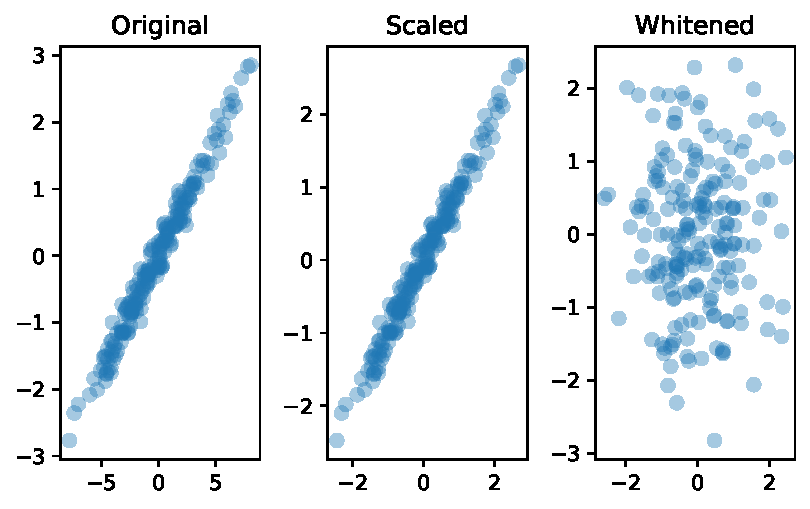
\includegraphics[keepaspectratio]{books/en-US/lab_files/figure-latex/cell-543-output-1.pdf}}

\begin{itemize}
\tightlist
\item
  Original: elongated ellipse.
\item
  Scaled: axis-aligned ellipse.
\item
  Whitened: circular cloud (uncorrelated, unit variance).
\end{itemize}

\subsubsection{Try It Yourself}\label{try-it-yourself-192}

\begin{enumerate}
\def\labelenumi{\arabic{enumi}.}
\tightlist
\item
  Add a third feature and apply centering, scaling, whitening.
\item
  Compare whitening with PCA - they use the same eigen-decomposition.
\item
  Test what happens if you skip centering before whitening.
\end{enumerate}

\subsubsection{The Takeaway}\label{the-takeaway-76}

\begin{itemize}
\tightlist
\item
  Centering → mean zero.
\item
  Scaling → unit variance.
\item
  Whitening → features uncorrelated, variance = 1. Linear algebra
  provides the exact matrix operations to make preprocessing systematic
  and reliable.
\end{itemize}

\subsection{95. Linear Regression and Classification (From Model to
Matrix)}\label{linear-regression-and-classification-from-model-to-matrix-1}

Linear regression and classification problems can be written neatly in
matrix form. This unifies data, models, and solutions under the
framework of least squares and linear decision boundaries.

\subsubsection{Linear Regression Model}\label{linear-regression-model}

For data \((x_i, y_i)\):

\[
y \approx X \beta
\]

\begin{itemize}
\tightlist
\item
  \(X\): design matrix (rows = samples, columns = features).
\item
  \(\beta\): coefficients to solve for.
\item
  Solution (least squares):
\end{itemize}

\[
\hat{\beta} = (X^T X)^{-1} X^T y
\]

\subsubsection{Set Up Your Lab}\label{set-up-your-lab-94}

\begin{Shaded}
\begin{Highlighting}[]
\ImportTok{import}\NormalTok{ numpy }\ImportTok{as}\NormalTok{ np}
\ImportTok{import}\NormalTok{ matplotlib.pyplot }\ImportTok{as}\NormalTok{ plt}
\ImportTok{from}\NormalTok{ sklearn.datasets }\ImportTok{import}\NormalTok{ make\_classification}
\end{Highlighting}
\end{Shaded}

\subsubsection{Step-by-Step Code
Walkthrough}\label{step-by-step-code-walkthrough-94}

\begin{enumerate}
\def\labelenumi{\arabic{enumi}.}
\tightlist
\item
  Linear regression example
\end{enumerate}

\begin{Shaded}
\begin{Highlighting}[]
\NormalTok{np.random.seed(}\DecValTok{0}\NormalTok{)}
\NormalTok{X }\OperatorTok{=}\NormalTok{ np.linspace(}\DecValTok{0}\NormalTok{, }\DecValTok{10}\NormalTok{, }\DecValTok{30}\NormalTok{).reshape(}\OperatorTok{{-}}\DecValTok{1}\NormalTok{,}\DecValTok{1}\NormalTok{)}
\NormalTok{y }\OperatorTok{=} \DecValTok{3}\OperatorTok{*}\NormalTok{X.squeeze() }\OperatorTok{+} \DecValTok{5} \OperatorTok{+}\NormalTok{ np.random.randn(}\DecValTok{30}\NormalTok{)}\OperatorTok{*}\DecValTok{2}
\end{Highlighting}
\end{Shaded}

Construct design matrix with bias term:

\begin{Shaded}
\begin{Highlighting}[]
\NormalTok{X\_design }\OperatorTok{=}\NormalTok{ np.column\_stack([np.ones\_like(X), X])}
\NormalTok{beta\_hat, }\OperatorTok{*}\NormalTok{\_ }\OperatorTok{=}\NormalTok{ np.linalg.lstsq(X\_design, y, rcond}\OperatorTok{=}\VariableTok{None}\NormalTok{)}
\BuiltInTok{print}\NormalTok{(}\StringTok{"Fitted coefficients:"}\NormalTok{, beta\_hat)}
\end{Highlighting}
\end{Shaded}

\begin{verbatim}
Fitted coefficients: [6.65833151 2.84547628]
\end{verbatim}

\begin{enumerate}
\def\labelenumi{\arabic{enumi}.}
\setcounter{enumi}{1}
\tightlist
\item
  Visualize regression line
\end{enumerate}

\begin{Shaded}
\begin{Highlighting}[]
\NormalTok{y\_pred }\OperatorTok{=}\NormalTok{ X\_design }\OperatorTok{@}\NormalTok{ beta\_hat}

\NormalTok{plt.scatter(X, y, label}\OperatorTok{=}\StringTok{"Data"}\NormalTok{)}
\NormalTok{plt.plot(X, y\_pred, }\StringTok{\textquotesingle{}r{-}\textquotesingle{}}\NormalTok{, label}\OperatorTok{=}\StringTok{"Fitted line"}\NormalTok{)}
\NormalTok{plt.legend()}
\NormalTok{plt.show()}
\end{Highlighting}
\end{Shaded}

\pandocbounded{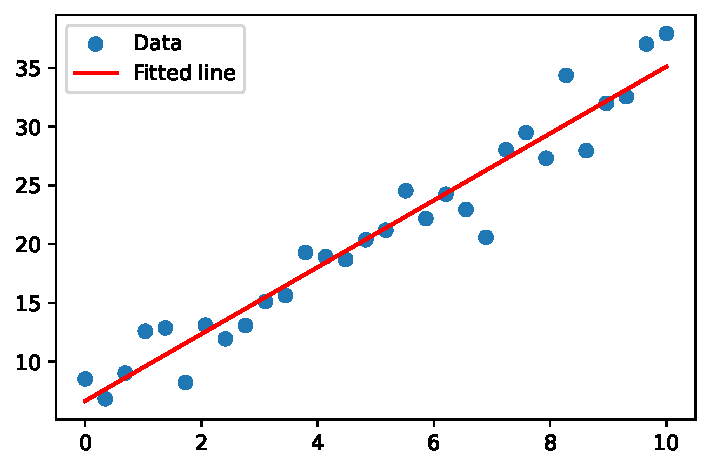
\includegraphics[keepaspectratio]{books/en-US/lab_files/figure-latex/cell-547-output-1.pdf}}

\begin{enumerate}
\def\labelenumi{\arabic{enumi}.}
\setcounter{enumi}{2}
\tightlist
\item
  Logistic classification with linear decision boundary
\end{enumerate}

\begin{Shaded}
\begin{Highlighting}[]
\NormalTok{Xc, yc }\OperatorTok{=}\NormalTok{ make\_classification(n\_features}\OperatorTok{=}\DecValTok{2}\NormalTok{, n\_redundant}\OperatorTok{=}\DecValTok{0}\NormalTok{, n\_informative}\OperatorTok{=}\DecValTok{2}\NormalTok{,}
\NormalTok{                             n\_clusters\_per\_class}\OperatorTok{=}\DecValTok{1}\NormalTok{, n\_samples}\OperatorTok{=}\DecValTok{100}\NormalTok{, random\_state}\OperatorTok{=}\DecValTok{0}\NormalTok{)}

\NormalTok{plt.scatter(Xc[:,}\DecValTok{0}\NormalTok{], Xc[:,}\DecValTok{1}\NormalTok{], c}\OperatorTok{=}\NormalTok{yc, cmap}\OperatorTok{=}\StringTok{"bwr"}\NormalTok{, alpha}\OperatorTok{=}\FloatTok{0.7}\NormalTok{)}
\NormalTok{plt.title(}\StringTok{"Classification data"}\NormalTok{)}
\NormalTok{plt.show()}
\end{Highlighting}
\end{Shaded}

\pandocbounded{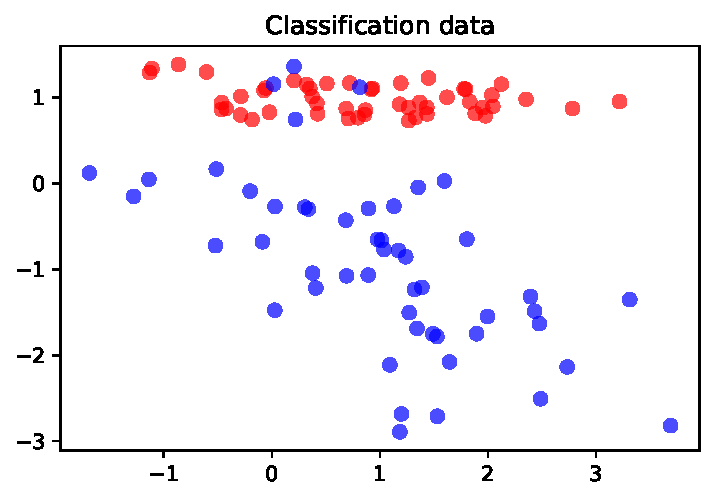
\includegraphics[keepaspectratio]{books/en-US/lab_files/figure-latex/cell-548-output-1.pdf}}

\begin{enumerate}
\def\labelenumi{\arabic{enumi}.}
\setcounter{enumi}{3}
\tightlist
\item
  Logistic regression via gradient descent
\end{enumerate}

\begin{Shaded}
\begin{Highlighting}[]
\KeywordTok{def}\NormalTok{ sigmoid(z):}
    \ControlFlowTok{return} \DecValTok{1}\OperatorTok{/}\NormalTok{(}\DecValTok{1}\OperatorTok{+}\NormalTok{np.exp(}\OperatorTok{{-}}\NormalTok{z))}

\NormalTok{X\_design }\OperatorTok{=}\NormalTok{ np.column\_stack([np.ones(}\BuiltInTok{len}\NormalTok{(Xc)), Xc])}
\NormalTok{y }\OperatorTok{=}\NormalTok{ yc}

\NormalTok{w }\OperatorTok{=}\NormalTok{ np.zeros(X\_design.shape[}\DecValTok{1}\NormalTok{])}
\NormalTok{lr }\OperatorTok{=} \FloatTok{0.1}

\ControlFlowTok{for}\NormalTok{ \_ }\KeywordTok{in} \BuiltInTok{range}\NormalTok{(}\DecValTok{2000}\NormalTok{):}
\NormalTok{    preds }\OperatorTok{=}\NormalTok{ sigmoid(X\_design }\OperatorTok{@}\NormalTok{ w)}
\NormalTok{    grad }\OperatorTok{=}\NormalTok{ X\_design.T }\OperatorTok{@}\NormalTok{ (preds }\OperatorTok{{-}}\NormalTok{ y) }\OperatorTok{/} \BuiltInTok{len}\NormalTok{(y)}
\NormalTok{    w }\OperatorTok{{-}=}\NormalTok{ lr }\OperatorTok{*}\NormalTok{ grad}

\BuiltInTok{print}\NormalTok{(}\StringTok{"Learned weights:"}\NormalTok{, w)}
\end{Highlighting}
\end{Shaded}

\begin{verbatim}
Learned weights: [-2.10451116  0.70752542  4.13295129]
\end{verbatim}

\begin{enumerate}
\def\labelenumi{\arabic{enumi}.}
\setcounter{enumi}{4}
\tightlist
\item
  Plot decision boundary
\end{enumerate}

\begin{Shaded}
\begin{Highlighting}[]
\NormalTok{xx, yy }\OperatorTok{=}\NormalTok{ np.meshgrid(np.linspace(Xc[:,}\DecValTok{0}\NormalTok{].}\BuiltInTok{min}\NormalTok{()}\OperatorTok{{-}}\DecValTok{1}\NormalTok{, Xc[:,}\DecValTok{0}\NormalTok{].}\BuiltInTok{max}\NormalTok{()}\OperatorTok{+}\DecValTok{1}\NormalTok{, }\DecValTok{200}\NormalTok{),}
\NormalTok{                     np.linspace(Xc[:,}\DecValTok{1}\NormalTok{].}\BuiltInTok{min}\NormalTok{()}\OperatorTok{{-}}\DecValTok{1}\NormalTok{, Xc[:,}\DecValTok{1}\NormalTok{].}\BuiltInTok{max}\NormalTok{()}\OperatorTok{+}\DecValTok{1}\NormalTok{, }\DecValTok{200}\NormalTok{))}

\NormalTok{grid }\OperatorTok{=}\NormalTok{ np.c\_[np.ones(xx.size), xx.ravel(), yy.ravel()]}
\NormalTok{probs }\OperatorTok{=}\NormalTok{ sigmoid(grid }\OperatorTok{@}\NormalTok{ w).reshape(xx.shape)}

\NormalTok{plt.contourf(xx, yy, probs, levels}\OperatorTok{=}\NormalTok{[}\DecValTok{0}\NormalTok{,}\FloatTok{0.5}\NormalTok{,}\DecValTok{1}\NormalTok{], alpha}\OperatorTok{=}\FloatTok{0.3}\NormalTok{, cmap}\OperatorTok{=}\StringTok{"bwr"}\NormalTok{)}
\NormalTok{plt.scatter(Xc[:,}\DecValTok{0}\NormalTok{], Xc[:,}\DecValTok{1}\NormalTok{], c}\OperatorTok{=}\NormalTok{yc, cmap}\OperatorTok{=}\StringTok{"bwr"}\NormalTok{, edgecolor}\OperatorTok{=}\StringTok{"k"}\NormalTok{)}
\NormalTok{plt.title(}\StringTok{"Linear decision boundary"}\NormalTok{)}
\NormalTok{plt.show()}
\end{Highlighting}
\end{Shaded}

\pandocbounded{\includegraphics[keepaspectratio]{books/en-US/lab_files/figure-latex/cell-550-output-1.pdf}}

\subsubsection{Try It Yourself}\label{try-it-yourself-193}

\begin{enumerate}
\def\labelenumi{\arabic{enumi}.}
\tightlist
\item
  Add polynomial features to regression and refit. Does the line bend
  into a curve?
\item
  Change learning rate in logistic regression - what happens?
\item
  Generate data that is not linearly separable. Can a linear model still
  classify well?
\end{enumerate}

\subsubsection{The Takeaway}\label{the-takeaway-77}

\begin{itemize}
\tightlist
\item
  Regression and classification fit naturally into linear algebra with
  matrix formulations.
\item
  Least squares solves regression directly; logistic regression requires
  optimization.
\item
  Linear models are simple, interpretable, and still form the foundation
  of modern machine learning.
\end{itemize}

\subsection{96. PCA in Practice (Dimensionality Reduction
Workflow)}\label{pca-in-practice-dimensionality-reduction-workflow-1}

Principal Component Analysis (PCA) is widely used to reduce dimensions,
compress data, and visualize high-dimensional datasets. Here, we'll walk
through a full PCA workflow: centering, computing components,
projecting, and visualizing.

\subsubsection{Set Up Your Lab}\label{set-up-your-lab-95}

\begin{Shaded}
\begin{Highlighting}[]
\ImportTok{import}\NormalTok{ numpy }\ImportTok{as}\NormalTok{ np}
\ImportTok{import}\NormalTok{ matplotlib.pyplot }\ImportTok{as}\NormalTok{ plt}
\ImportTok{from}\NormalTok{ sklearn.datasets }\ImportTok{import}\NormalTok{ load\_digits}
\end{Highlighting}
\end{Shaded}

\subsubsection{Step-by-Step Code
Walkthrough}\label{step-by-step-code-walkthrough-95}

\begin{enumerate}
\def\labelenumi{\arabic{enumi}.}
\tightlist
\item
  Load dataset (digits)
\end{enumerate}

\begin{Shaded}
\begin{Highlighting}[]
\NormalTok{digits }\OperatorTok{=}\NormalTok{ load\_digits()}
\NormalTok{X }\OperatorTok{=}\NormalTok{ digits.data  }\CommentTok{\# shape (1797, 64)}
\NormalTok{y }\OperatorTok{=}\NormalTok{ digits.target}
\BuiltInTok{print}\NormalTok{(}\StringTok{"Data shape:"}\NormalTok{, X.shape)}
\end{Highlighting}
\end{Shaded}

\begin{verbatim}
Data shape: (1797, 64)
\end{verbatim}

Each sample is an 8×8 grayscale image flattened into 64 features.

\begin{enumerate}
\def\labelenumi{\arabic{enumi}.}
\setcounter{enumi}{1}
\tightlist
\item
  Center the data
\end{enumerate}

\begin{Shaded}
\begin{Highlighting}[]
\NormalTok{X\_centered }\OperatorTok{=}\NormalTok{ X }\OperatorTok{{-}}\NormalTok{ X.mean(axis}\OperatorTok{=}\DecValTok{0}\NormalTok{)}
\end{Highlighting}
\end{Shaded}

\begin{enumerate}
\def\labelenumi{\arabic{enumi}.}
\setcounter{enumi}{2}
\tightlist
\item
  Compute PCA via SVD
\end{enumerate}

\begin{Shaded}
\begin{Highlighting}[]
\NormalTok{U, S, Vt }\OperatorTok{=}\NormalTok{ np.linalg.svd(X\_centered, full\_matrices}\OperatorTok{=}\VariableTok{False}\NormalTok{)}
\NormalTok{explained\_variance }\OperatorTok{=}\NormalTok{ (S}\OperatorTok{**}\DecValTok{2}\NormalTok{) }\OperatorTok{/}\NormalTok{ (}\BuiltInTok{len}\NormalTok{(X) }\OperatorTok{{-}} \DecValTok{1}\NormalTok{)}
\NormalTok{explained\_ratio }\OperatorTok{=}\NormalTok{ explained\_variance }\OperatorTok{/}\NormalTok{ explained\_variance.}\BuiltInTok{sum}\NormalTok{()}
\end{Highlighting}
\end{Shaded}

\begin{enumerate}
\def\labelenumi{\arabic{enumi}.}
\setcounter{enumi}{3}
\tightlist
\item
  Plot explained variance ratio
\end{enumerate}

\begin{Shaded}
\begin{Highlighting}[]
\NormalTok{plt.plot(np.cumsum(explained\_ratio[:}\DecValTok{30}\NormalTok{]), }\StringTok{\textquotesingle{}o{-}\textquotesingle{}}\NormalTok{)}
\NormalTok{plt.xlabel(}\StringTok{"Number of components"}\NormalTok{)}
\NormalTok{plt.ylabel(}\StringTok{"Cumulative explained variance"}\NormalTok{)}
\NormalTok{plt.title(}\StringTok{"PCA explained variance"}\NormalTok{)}
\NormalTok{plt.grid(}\VariableTok{True}\NormalTok{)}
\NormalTok{plt.show()}
\end{Highlighting}
\end{Shaded}

\pandocbounded{\includegraphics[keepaspectratio]{books/en-US/lab_files/figure-latex/cell-555-output-1.pdf}}

This shows how many components are needed to capture most variance.

\begin{enumerate}
\def\labelenumi{\arabic{enumi}.}
\setcounter{enumi}{4}
\tightlist
\item
  Project onto top 2 components for visualization
\end{enumerate}

\begin{Shaded}
\begin{Highlighting}[]
\NormalTok{X\_pca2 }\OperatorTok{=}\NormalTok{ X\_centered }\OperatorTok{@}\NormalTok{ Vt[:}\DecValTok{2}\NormalTok{].T}
\NormalTok{plt.scatter(X\_pca2[:,}\DecValTok{0}\NormalTok{], X\_pca2[:,}\DecValTok{1}\NormalTok{], c}\OperatorTok{=}\NormalTok{y, cmap}\OperatorTok{=}\StringTok{"tab10"}\NormalTok{, alpha}\OperatorTok{=}\FloatTok{0.6}\NormalTok{, s}\OperatorTok{=}\DecValTok{15}\NormalTok{)}
\NormalTok{plt.colorbar()}
\NormalTok{plt.title(}\StringTok{"Digits dataset (PCA 2D projection)"}\NormalTok{)}
\NormalTok{plt.show()}
\end{Highlighting}
\end{Shaded}

\pandocbounded{\includegraphics[keepaspectratio]{books/en-US/lab_files/figure-latex/cell-556-output-1.pdf}}

\begin{enumerate}
\def\labelenumi{\arabic{enumi}.}
\setcounter{enumi}{5}
\tightlist
\item
  Reconstruct images from reduced dimensions
\end{enumerate}

\begin{Shaded}
\begin{Highlighting}[]
\NormalTok{k }\OperatorTok{=} \DecValTok{20}
\NormalTok{X\_pca20 }\OperatorTok{=}\NormalTok{ X\_centered }\OperatorTok{@}\NormalTok{ Vt[:k].T}
\NormalTok{X\_reconstructed }\OperatorTok{=}\NormalTok{ X\_pca20 }\OperatorTok{@}\NormalTok{ Vt[:k]}

\NormalTok{fig, axes }\OperatorTok{=}\NormalTok{ plt.subplots(}\DecValTok{2}\NormalTok{, }\DecValTok{10}\NormalTok{, figsize}\OperatorTok{=}\NormalTok{(}\DecValTok{10}\NormalTok{,}\DecValTok{2}\NormalTok{))}
\ControlFlowTok{for}\NormalTok{ i }\KeywordTok{in} \BuiltInTok{range}\NormalTok{(}\DecValTok{10}\NormalTok{):}
\NormalTok{    axes[}\DecValTok{0}\NormalTok{,i].imshow(X[i].reshape(}\DecValTok{8}\NormalTok{,}\DecValTok{8}\NormalTok{), cmap}\OperatorTok{=}\StringTok{"gray"}\NormalTok{)}
\NormalTok{    axes[}\DecValTok{0}\NormalTok{,i].axis(}\StringTok{"off"}\NormalTok{)}
\NormalTok{    axes[}\DecValTok{1}\NormalTok{,i].imshow(X\_reconstructed[i].reshape(}\DecValTok{8}\NormalTok{,}\DecValTok{8}\NormalTok{), cmap}\OperatorTok{=}\StringTok{"gray"}\NormalTok{)}
\NormalTok{    axes[}\DecValTok{1}\NormalTok{,i].axis(}\StringTok{"off"}\NormalTok{)}
\NormalTok{plt.suptitle(}\StringTok{"Original (top) vs PCA reconstruction (bottom, 20 comps)"}\NormalTok{)}
\NormalTok{plt.show()}
\end{Highlighting}
\end{Shaded}

\pandocbounded{\includegraphics[keepaspectratio]{books/en-US/lab_files/figure-latex/cell-557-output-1.pdf}}

Even with only 20/64 components, the digits remain recognizable.

\subsubsection{Try It Yourself}\label{try-it-yourself-194}

\begin{enumerate}
\def\labelenumi{\arabic{enumi}.}
\tightlist
\item
  Change \(k\) to 5, 10, 30 - how do reconstructions change?
\item
  Use top 2 PCA components to classify digits with k-NN. How does
  accuracy compare to full 64 features?
\item
  Try PCA on your own dataset (images, tabular data).
\end{enumerate}

\subsubsection{The Takeaway}\label{the-takeaway-78}

\begin{itemize}
\tightlist
\item
  PCA reduces dimensions while keeping maximum variance.
\item
  In practice: center → decompose → select top components →
  project/reconstruct.
\item
  PCA enables visualization, compression, and denoising in real-world
  workflows.
\end{itemize}

\subsection{97. Recommender Systems and Low-Rank Models (Fill the
Missing
Entries)}\label{recommender-systems-and-low-rank-models-fill-the-missing-entries-1}

Recommender systems often deal with incomplete matrices - rows are
users, columns are items, entries are ratings. Most entries are missing,
but the matrix is usually close to low-rank (because user preferences
depend on only a few hidden factors). SVD and low-rank approximations
are powerful tools to fill in these missing values.

\subsubsection{Set Up Your Lab}\label{set-up-your-lab-96}

\begin{Shaded}
\begin{Highlighting}[]
\ImportTok{import}\NormalTok{ numpy }\ImportTok{as}\NormalTok{ np}
\ImportTok{import}\NormalTok{ matplotlib.pyplot }\ImportTok{as}\NormalTok{ plt}
\end{Highlighting}
\end{Shaded}

\subsubsection{Step-by-Step Code
Walkthrough}\label{step-by-step-code-walkthrough-96}

\begin{enumerate}
\def\labelenumi{\arabic{enumi}.}
\tightlist
\item
  Simulate a user--item rating matrix
\end{enumerate}

\begin{Shaded}
\begin{Highlighting}[]
\NormalTok{np.random.seed(}\DecValTok{0}\NormalTok{)}
\NormalTok{true\_users }\OperatorTok{=}\NormalTok{ np.random.randn(}\DecValTok{10}\NormalTok{, }\DecValTok{3}\NormalTok{)   }\CommentTok{\# 10 users, 3 latent features}
\NormalTok{true\_items }\OperatorTok{=}\NormalTok{ np.random.randn(}\DecValTok{3}\NormalTok{, }\DecValTok{8}\NormalTok{)    }\CommentTok{\# 8 items}
\NormalTok{R\_full }\OperatorTok{=}\NormalTok{ true\_users }\OperatorTok{@}\NormalTok{ true\_items      }\CommentTok{\# true low{-}rank ratings}
\end{Highlighting}
\end{Shaded}

\begin{enumerate}
\def\labelenumi{\arabic{enumi}.}
\setcounter{enumi}{1}
\tightlist
\item
  Hide some ratings (simulate missing data)
\end{enumerate}

\begin{Shaded}
\begin{Highlighting}[]
\NormalTok{mask }\OperatorTok{=}\NormalTok{ np.random.rand(}\OperatorTok{*}\NormalTok{R\_full.shape) }\OperatorTok{\textgreater{}} \FloatTok{0.3}  \CommentTok{\# keep 70\% of entries}
\NormalTok{R\_obs }\OperatorTok{=}\NormalTok{ np.where(mask, R\_full, np.nan)}

\BuiltInTok{print}\NormalTok{(}\StringTok{"Observed ratings:}\CharTok{\textbackslash{}n}\StringTok{"}\NormalTok{, R\_obs)}
\end{Highlighting}
\end{Shaded}

\begin{verbatim}
Observed ratings:
 [[-1.10781465         nan -3.56526968         nan -2.1729387   1.43510077
   1.46641178  0.79023284]
 [ 0.84819453         nan         nan         nan         nan         nan
   2.30434358  3.03008138]
 [        nan  0.32479187 -0.51818422         nan  0.02013802         nan
   1.29874918  1.33053637]
 [-1.81407786  1.24241182         nan -1.32723907         nan         nan
  -0.31110699         nan]
 [-0.48527696         nan -1.51957106         nan -0.86984941  0.52807989
          nan  0.33771451]
 [-0.26997359 -0.48498966         nan -2.73891459 -2.48167957  2.88740609
  -0.24614835         nan]
 [ 3.57769701 -1.608339    4.73789234  1.13583164  3.63451505 -2.60495928
   2.12453635  3.76472563]
 [ 0.69623809 -0.59117353 -0.28890188 -2.36431192         nan  1.50136796
   0.74268078         nan]
 [ 0.85768141  1.33357168         nan         nan  1.65089037 -2.46456289
   3.51030491  3.31220347]
 [-2.463496    0.60826298 -3.81241599 -2.11839267 -3.86597359  3.52934055
  -1.76203083 -2.63130953]]
\end{verbatim}

\begin{enumerate}
\def\labelenumi{\arabic{enumi}.}
\setcounter{enumi}{2}
\tightlist
\item
  Simple mean imputation (baseline)
\end{enumerate}

\begin{Shaded}
\begin{Highlighting}[]
\NormalTok{R\_mean }\OperatorTok{=}\NormalTok{ np.where(np.isnan(R\_obs), np.nanmean(R\_obs), R\_obs)}
\end{Highlighting}
\end{Shaded}

\begin{enumerate}
\def\labelenumi{\arabic{enumi}.}
\setcounter{enumi}{3}
\tightlist
\item
  Apply SVD for low-rank approximation
\end{enumerate}

\begin{Shaded}
\begin{Highlighting}[]
\CommentTok{\# Replace NaNs with zeros for SVD step}
\NormalTok{R\_filled }\OperatorTok{=}\NormalTok{ np.nan\_to\_num(R\_obs, nan}\OperatorTok{=}\FloatTok{0.0}\NormalTok{)}

\NormalTok{U, S, Vt }\OperatorTok{=}\NormalTok{ np.linalg.svd(R\_filled, full\_matrices}\OperatorTok{=}\VariableTok{False}\NormalTok{)}

\NormalTok{k }\OperatorTok{=} \DecValTok{3}  \CommentTok{\# latent dimension}
\NormalTok{R\_approx }\OperatorTok{=}\NormalTok{ U[:, :k] }\OperatorTok{@}\NormalTok{ np.diag(S[:k]) }\OperatorTok{@}\NormalTok{ Vt[:k, :]}
\end{Highlighting}
\end{Shaded}

\begin{enumerate}
\def\labelenumi{\arabic{enumi}.}
\setcounter{enumi}{4}
\tightlist
\item
  Compare filled matrix with ground truth
\end{enumerate}

\begin{Shaded}
\begin{Highlighting}[]
\NormalTok{error }\OperatorTok{=}\NormalTok{ np.nanmean((R\_full }\OperatorTok{{-}}\NormalTok{ R\_approx)}\OperatorTok{**}\DecValTok{2}\NormalTok{)}
\BuiltInTok{print}\NormalTok{(}\StringTok{"Approximation error (MSE):"}\NormalTok{, error)}
\end{Highlighting}
\end{Shaded}

\begin{verbatim}
Approximation error (MSE): 1.4862378490976202
\end{verbatim}

\begin{enumerate}
\def\labelenumi{\arabic{enumi}.}
\setcounter{enumi}{5}
\tightlist
\item
  Visualize original vs reconstructed
\end{enumerate}

\begin{Shaded}
\begin{Highlighting}[]
\NormalTok{fig, axes }\OperatorTok{=}\NormalTok{ plt.subplots(}\DecValTok{1}\NormalTok{, }\DecValTok{2}\NormalTok{, figsize}\OperatorTok{=}\NormalTok{(}\DecValTok{8}\NormalTok{,}\DecValTok{4}\NormalTok{))}
\NormalTok{axes[}\DecValTok{0}\NormalTok{].imshow(R\_full, cmap}\OperatorTok{=}\StringTok{"viridis"}\NormalTok{)}
\NormalTok{axes[}\DecValTok{0}\NormalTok{].set\_title(}\StringTok{"True ratings"}\NormalTok{)}
\NormalTok{axes[}\DecValTok{1}\NormalTok{].imshow(R\_approx, cmap}\OperatorTok{=}\StringTok{"viridis"}\NormalTok{)}
\NormalTok{axes[}\DecValTok{1}\NormalTok{].set\_title(}\StringTok{"Low{-}rank approximation"}\NormalTok{)}
\NormalTok{plt.show()}
\end{Highlighting}
\end{Shaded}

\pandocbounded{\includegraphics[keepaspectratio]{books/en-US/lab_files/figure-latex/cell-564-output-1.pdf}}

\subsubsection{Try It Yourself}\label{try-it-yourself-195}

\begin{enumerate}
\def\labelenumi{\arabic{enumi}.}
\tightlist
\item
  Vary \(k\) (2, 3, 5). Does error go down?
\item
  Mask more entries (50\%, 80\%) - how does SVD reconstruction perform?
\item
  Use iterative imputation: alternate filling missing entries with
  low-rank approximations.
\end{enumerate}

\subsubsection{The Takeaway}\label{the-takeaway-79}

\begin{itemize}
\tightlist
\item
  Recommender systems rely on low-rank structure of user--item matrices.
\item
  SVD provides a natural way to approximate and fill missing ratings.
\item
  This low-rank modeling idea underpins modern collaborative filtering
  systems like Netflix and Spotify recommenders.
\end{itemize}

\subsection{98. PageRank and Random Walks (Ranking with
Eigenvectors)}\label{pagerank-and-random-walks-ranking-with-eigenvectors-1}

The PageRank algorithm, made famous by Google, uses linear algebra and
random walks on graphs to rank nodes (webpages, people, items). The
idea: importance flows through links - being linked by important nodes
makes you important.

\subsubsection{The PageRank Idea}\label{the-pagerank-idea}

\begin{itemize}
\tightlist
\item
  Start a random walk on a graph: at each step, move to a random
  neighbor.
\item
  Add a ``teleportation'' step with probability \(1 - \alpha\) to avoid
  dead ends.
\item
  The steady-state distribution of this walk is the PageRank vector,
  found as the principal eigenvector of the transition matrix.
\end{itemize}

\subsubsection{Set Up Your Lab}\label{set-up-your-lab-97}

\begin{Shaded}
\begin{Highlighting}[]
\ImportTok{import}\NormalTok{ numpy }\ImportTok{as}\NormalTok{ np}
\ImportTok{import}\NormalTok{ networkx }\ImportTok{as}\NormalTok{ nx}
\ImportTok{import}\NormalTok{ matplotlib.pyplot }\ImportTok{as}\NormalTok{ plt}
\end{Highlighting}
\end{Shaded}

\subsubsection{Step-by-Step Code
Walkthrough}\label{step-by-step-code-walkthrough-97}

\begin{enumerate}
\def\labelenumi{\arabic{enumi}.}
\tightlist
\item
  Build a small directed graph
\end{enumerate}

\begin{Shaded}
\begin{Highlighting}[]
\NormalTok{G }\OperatorTok{=}\NormalTok{ nx.DiGraph()}
\NormalTok{G.add\_edges\_from([}
\NormalTok{    (}\DecValTok{0}\NormalTok{,}\DecValTok{1}\NormalTok{), (}\DecValTok{1}\NormalTok{,}\DecValTok{2}\NormalTok{), (}\DecValTok{2}\NormalTok{,}\DecValTok{0}\NormalTok{),  }\CommentTok{\# cycle among 0–1–2}
\NormalTok{    (}\DecValTok{2}\NormalTok{,}\DecValTok{3}\NormalTok{), (}\DecValTok{3}\NormalTok{,}\DecValTok{2}\NormalTok{),         }\CommentTok{\# back{-}and{-}forth 2–3}
\NormalTok{    (}\DecValTok{1}\NormalTok{,}\DecValTok{3}\NormalTok{), (}\DecValTok{3}\NormalTok{,}\DecValTok{4}\NormalTok{), (}\DecValTok{4}\NormalTok{,}\DecValTok{1}\NormalTok{)   }\CommentTok{\# small loop with 1–3–4}
\NormalTok{])}
\NormalTok{nx.draw\_circular(G, with\_labels}\OperatorTok{=}\VariableTok{True}\NormalTok{, node\_color}\OperatorTok{=}\StringTok{"lightblue"}\NormalTok{, node\_size}\OperatorTok{=}\DecValTok{800}\NormalTok{, arrowsize}\OperatorTok{=}\DecValTok{15}\NormalTok{)}
\NormalTok{plt.show()}
\end{Highlighting}
\end{Shaded}

\pandocbounded{\includegraphics[keepaspectratio]{books/en-US/lab_files/figure-latex/cell-566-output-1.pdf}}

\begin{enumerate}
\def\labelenumi{\arabic{enumi}.}
\setcounter{enumi}{1}
\tightlist
\item
  Build adjacency and transition matrix
\end{enumerate}

\begin{Shaded}
\begin{Highlighting}[]
\NormalTok{n }\OperatorTok{=}\NormalTok{ G.number\_of\_nodes()}
\NormalTok{A }\OperatorTok{=}\NormalTok{ nx.to\_numpy\_array(G, nodelist}\OperatorTok{=}\BuiltInTok{range}\NormalTok{(n))}
\NormalTok{P }\OperatorTok{=}\NormalTok{ A }\OperatorTok{/}\NormalTok{ A.}\BuiltInTok{sum}\NormalTok{(axis}\OperatorTok{=}\DecValTok{1}\NormalTok{, keepdims}\OperatorTok{=}\VariableTok{True}\NormalTok{)  }\CommentTok{\# row{-}stochastic transition matrix}
\end{Highlighting}
\end{Shaded}

\begin{enumerate}
\def\labelenumi{\arabic{enumi}.}
\setcounter{enumi}{2}
\tightlist
\item
  Add teleportation (Google matrix)
\end{enumerate}

\begin{Shaded}
\begin{Highlighting}[]
\NormalTok{alpha }\OperatorTok{=} \FloatTok{0.85}  \CommentTok{\# damping factor}
\NormalTok{G\_matrix }\OperatorTok{=}\NormalTok{ alpha }\OperatorTok{*}\NormalTok{ P }\OperatorTok{+}\NormalTok{ (}\DecValTok{1} \OperatorTok{{-}}\NormalTok{ alpha) }\OperatorTok{*}\NormalTok{ np.ones((n,n)) }\OperatorTok{/}\NormalTok{ n}
\end{Highlighting}
\end{Shaded}

\begin{enumerate}
\def\labelenumi{\arabic{enumi}.}
\setcounter{enumi}{3}
\tightlist
\item
  Power iteration to compute PageRank
\end{enumerate}

\begin{Shaded}
\begin{Highlighting}[]
\NormalTok{r }\OperatorTok{=}\NormalTok{ np.ones(n) }\OperatorTok{/}\NormalTok{ n  }\CommentTok{\# start uniform}
\ControlFlowTok{for}\NormalTok{ \_ }\KeywordTok{in} \BuiltInTok{range}\NormalTok{(}\DecValTok{100}\NormalTok{):}
\NormalTok{    r }\OperatorTok{=}\NormalTok{ r }\OperatorTok{@}\NormalTok{ G\_matrix}
\NormalTok{r }\OperatorTok{/=}\NormalTok{ r.}\BuiltInTok{sum}\NormalTok{()}
\BuiltInTok{print}\NormalTok{(}\StringTok{"PageRank vector:"}\NormalTok{, r)}
\end{Highlighting}
\end{Shaded}

\begin{verbatim}
PageRank vector: [0.13219034 0.25472358 0.24044787 0.24044787 0.13219034]
\end{verbatim}

\begin{enumerate}
\def\labelenumi{\arabic{enumi}.}
\setcounter{enumi}{4}
\tightlist
\item
  Compare with NetworkX built-in
\end{enumerate}

\begin{Shaded}
\begin{Highlighting}[]
\NormalTok{pr }\OperatorTok{=}\NormalTok{ nx.pagerank(G, alpha}\OperatorTok{=}\NormalTok{alpha)}
\BuiltInTok{print}\NormalTok{(}\StringTok{"NetworkX PageRank:"}\NormalTok{, pr)}
\end{Highlighting}
\end{Shaded}

\begin{verbatim}
NetworkX PageRank: {0: 0.13219008157546333, 1: 0.2547244023837789, 2: 0.24044771723264727, 3: 0.24044771723264727, 4: 0.13219008157546333}
\end{verbatim}

\begin{enumerate}
\def\labelenumi{\arabic{enumi}.}
\setcounter{enumi}{5}
\tightlist
\item
  Visualize node importance
\end{enumerate}

\begin{Shaded}
\begin{Highlighting}[]
\NormalTok{sizes }\OperatorTok{=}\NormalTok{ [}\DecValTok{5000} \OperatorTok{*}\NormalTok{ r\_i }\ControlFlowTok{for}\NormalTok{ r\_i }\KeywordTok{in}\NormalTok{ r]}
\NormalTok{nx.draw\_circular(G, with\_labels}\OperatorTok{=}\VariableTok{True}\NormalTok{, node\_size}\OperatorTok{=}\NormalTok{sizes, node\_color}\OperatorTok{=}\StringTok{"lightblue"}\NormalTok{, arrowsize}\OperatorTok{=}\DecValTok{15}\NormalTok{)}
\NormalTok{plt.title(}\StringTok{"PageRank visualization (node size \textasciitilde{} importance)"}\NormalTok{)}
\NormalTok{plt.show()}
\end{Highlighting}
\end{Shaded}

\pandocbounded{\includegraphics[keepaspectratio]{books/en-US/lab_files/figure-latex/cell-571-output-1.pdf}}

\subsubsection{Try It Yourself}\label{try-it-yourself-196}

\begin{enumerate}
\def\labelenumi{\arabic{enumi}.}
\tightlist
\item
  Change \(\alpha\) (e.g., 0.6 vs 0.95). Does ranking change?
\item
  Add a ``dangling node'' with no outlinks. How does teleportation
  handle it?
\item
  Try PageRank on a larger graph (like a random graph with 50 nodes).
\end{enumerate}

\subsubsection{The Takeaway}\label{the-takeaway-80}

\begin{itemize}
\tightlist
\item
  PageRank is a random-walk steady state problem.
\item
  It reduces to finding the dominant eigenvector of the Google matrix.
\item
  This method generalizes beyond webpages - to influence ranking,
  recommendation, and network analysis.
\end{itemize}

\subsection{99. Numerical Linear Algebra Essentials (Floating Point,
BLAS/LAPACK)}\label{numerical-linear-algebra-essentials-floating-point-blaslapack-1}

When working with linear algebra on computers, numbers are not exact.
They live in floating-point arithmetic, and computations rely on highly
optimized libraries like BLAS and LAPACK. Understanding these essentials
is crucial to doing linear algebra at scale.

\subsubsection{Floating Point Basics}\label{floating-point-basics}

\begin{itemize}
\item
  Numbers are stored in base-2 scientific notation:

  \[
  x = \pm (1.b_1b_2b_3\ldots) \times 2^e
  \]
\item
  Limited precision means rounding errors.
\item
  Two key constants:

  \begin{itemize}
  \tightlist
  \item
    Machine epsilon
    (\$\epsilon \(): smallest difference detectable (\)\approx 10\^{}\{-16\}\$
    for double).
  \item
    Overflow/underflow: too large or too small to represent.
  \end{itemize}
\end{itemize}

\subsubsection{Set Up Your Lab}\label{set-up-your-lab-98}

\begin{Shaded}
\begin{Highlighting}[]
\ImportTok{import}\NormalTok{ numpy }\ImportTok{as}\NormalTok{ np}
\end{Highlighting}
\end{Shaded}

\subsubsection{Step-by-Step Code
Walkthrough}\label{step-by-step-code-walkthrough-98}

\begin{enumerate}
\def\labelenumi{\arabic{enumi}.}
\tightlist
\item
  Machine epsilon
\end{enumerate}

\begin{Shaded}
\begin{Highlighting}[]
\NormalTok{eps }\OperatorTok{=}\NormalTok{ np.finfo(}\BuiltInTok{float}\NormalTok{).eps}
\BuiltInTok{print}\NormalTok{(}\StringTok{"Machine epsilon:"}\NormalTok{, eps)}
\end{Highlighting}
\end{Shaded}

\begin{verbatim}
Machine epsilon: 2.220446049250313e-16
\end{verbatim}

\begin{enumerate}
\def\labelenumi{\arabic{enumi}.}
\setcounter{enumi}{1}
\tightlist
\item
  Round-off error demo
\end{enumerate}

\begin{Shaded}
\begin{Highlighting}[]
\NormalTok{a }\OperatorTok{=} \FloatTok{1e16}
\NormalTok{b }\OperatorTok{=} \FloatTok{1.0}
\BuiltInTok{print}\NormalTok{(}\StringTok{"a + b {-} a:"}\NormalTok{, (a }\OperatorTok{+}\NormalTok{ b) }\OperatorTok{{-}}\NormalTok{ a)  }\CommentTok{\# may lose b due to precision limits}
\end{Highlighting}
\end{Shaded}

\begin{verbatim}
a + b - a: 0.0
\end{verbatim}

\begin{enumerate}
\def\labelenumi{\arabic{enumi}.}
\setcounter{enumi}{2}
\tightlist
\item
  Stability of matrix inversion
\end{enumerate}

\begin{Shaded}
\begin{Highlighting}[]
\NormalTok{A }\OperatorTok{=}\NormalTok{ np.array([[}\DecValTok{1}\NormalTok{, }\FloatTok{1.0001}\NormalTok{], [}\FloatTok{1.0001}\NormalTok{, }\DecValTok{1}\NormalTok{]])}
\NormalTok{b }\OperatorTok{=}\NormalTok{ np.array([}\DecValTok{2}\NormalTok{, }\FloatTok{2.0001}\NormalTok{])}

\NormalTok{x\_direct }\OperatorTok{=}\NormalTok{ np.linalg.solve(A, b)}
\NormalTok{x\_via\_inv }\OperatorTok{=}\NormalTok{ np.linalg.inv(A) }\OperatorTok{@}\NormalTok{ b}

\BuiltInTok{print}\NormalTok{(}\StringTok{"Solve:"}\NormalTok{, x\_direct)}
\BuiltInTok{print}\NormalTok{(}\StringTok{"Inverse method:"}\NormalTok{, x\_via\_inv)}
\end{Highlighting}
\end{Shaded}

\begin{verbatim}
Solve: [1.499975 0.499975]
Inverse method: [1.499975 0.499975]
\end{verbatim}

Notice: using \texttt{np.linalg.inv} can be less stable - better to
solve directly.

\begin{enumerate}
\def\labelenumi{\arabic{enumi}.}
\setcounter{enumi}{3}
\tightlist
\item
  Conditioning of a matrix
\end{enumerate}

\begin{Shaded}
\begin{Highlighting}[]
\NormalTok{cond }\OperatorTok{=}\NormalTok{ np.linalg.cond(A)}
\BuiltInTok{print}\NormalTok{(}\StringTok{"Condition number:"}\NormalTok{, cond)}
\end{Highlighting}
\end{Shaded}

\begin{verbatim}
Condition number: 20001.00000000417
\end{verbatim}

\begin{itemize}
\tightlist
\item
  Large condition number → small input changes cause big output changes.
\end{itemize}

\begin{enumerate}
\def\labelenumi{\arabic{enumi}.}
\setcounter{enumi}{4}
\tightlist
\item
  BLAS/LAPACK under the hood
\end{enumerate}

\begin{Shaded}
\begin{Highlighting}[]
\NormalTok{A }\OperatorTok{=}\NormalTok{ np.random.randn(}\DecValTok{500}\NormalTok{, }\DecValTok{500}\NormalTok{)}
\NormalTok{B }\OperatorTok{=}\NormalTok{ np.random.randn(}\DecValTok{500}\NormalTok{, }\DecValTok{500}\NormalTok{)}

\CommentTok{\# Matrix multiplication (calls optimized BLAS under the hood)}
\NormalTok{C }\OperatorTok{=}\NormalTok{ A }\OperatorTok{@}\NormalTok{ B}
\end{Highlighting}
\end{Shaded}

This \texttt{@} operator is not a naive loop - it calls a highly
optimized C/Fortran routine.

\subsubsection{Try It Yourself}\label{try-it-yourself-197}

\begin{enumerate}
\def\labelenumi{\arabic{enumi}.}
\tightlist
\item
  Compare solving \texttt{Ax\ =\ b} with \texttt{np.linalg.solve} vs
  \texttt{np.linalg.inv(A)\ @\ b} for larger, ill-conditioned systems.
\item
  Use \texttt{np.linalg.svd} on a nearly singular matrix. How stable are
  the singular values?
\item
  Check performance: time \texttt{A\ @\ B} for sizes 100, 500, 1000.
\end{enumerate}

\subsubsection{The Takeaway}\label{the-takeaway-81}

\begin{itemize}
\tightlist
\item
  Numerical linear algebra = math + floating-point reality.
\item
  Always prefer stable algorithms (\texttt{solve}, \texttt{qr},
  \texttt{svd}) over naive inversion.
\item
  Libraries like BLAS/LAPACK make large computations fast, but
  understanding precision and conditioning prevents nasty surprises.
\end{itemize}

\subsection{100. Capstone Problem Sets and Next Steps (A Roadmap to
Mastery)}\label{capstone-problem-sets-and-next-steps-a-roadmap-to-mastery-1}

This final section ties everything together. Instead of introducing a
new topic, it provides capstone labs that combine multiple ideas from
the book. Working through them will give you confidence that you can
apply linear algebra to real problems.

\subsubsection{Problem Set 1 - Image Compression with
SVD}\label{problem-set-1---image-compression-with-svd}

Take an image, treat it as a matrix, and approximate it with low-rank
SVD.

\begin{Shaded}
\begin{Highlighting}[]
\ImportTok{import}\NormalTok{ numpy }\ImportTok{as}\NormalTok{ np}
\ImportTok{import}\NormalTok{ matplotlib.pyplot }\ImportTok{as}\NormalTok{ plt}
\ImportTok{from}\NormalTok{ skimage }\ImportTok{import}\NormalTok{ data, color}

\CommentTok{\# Load grayscale image}
\NormalTok{img }\OperatorTok{=}\NormalTok{ color.rgb2gray(data.astronaut())}
\NormalTok{U, S, Vt }\OperatorTok{=}\NormalTok{ np.linalg.svd(img, full\_matrices}\OperatorTok{=}\VariableTok{False}\NormalTok{)}

\CommentTok{\# Approximate with rank{-}k}
\NormalTok{k }\OperatorTok{=} \DecValTok{50}
\NormalTok{img\_approx }\OperatorTok{=}\NormalTok{ U[:, :k] }\OperatorTok{@}\NormalTok{ np.diag(S[:k]) }\OperatorTok{@}\NormalTok{ Vt[:k, :]}

\NormalTok{plt.subplot(}\DecValTok{1}\NormalTok{,}\DecValTok{2}\NormalTok{,}\DecValTok{1}\NormalTok{)}
\NormalTok{plt.imshow(img, cmap}\OperatorTok{=}\StringTok{"gray"}\NormalTok{)}
\NormalTok{plt.title(}\StringTok{"Original"}\NormalTok{)}
\NormalTok{plt.axis(}\StringTok{"off"}\NormalTok{)}

\NormalTok{plt.subplot(}\DecValTok{1}\NormalTok{,}\DecValTok{2}\NormalTok{,}\DecValTok{2}\NormalTok{)}
\NormalTok{plt.imshow(img\_approx, cmap}\OperatorTok{=}\StringTok{"gray"}\NormalTok{)}
\NormalTok{plt.title(}\SpecialStringTok{f"Rank{-}}\SpecialCharTok{\{}\NormalTok{k}\SpecialCharTok{\}}\SpecialStringTok{ Approximation"}\NormalTok{)}
\NormalTok{plt.axis(}\StringTok{"off"}\NormalTok{)}

\NormalTok{plt.show()}
\end{Highlighting}
\end{Shaded}

\pandocbounded{\includegraphics[keepaspectratio]{books/en-US/lab_files/figure-latex/cell-578-output-1.pdf}}

Try different \(k\) values (5, 20, 100). How does quality
vs.~compression trade off?

\subsubsection{Problem Set 2 - Predictive Modeling with PCA +
Regression}\label{problem-set-2---predictive-modeling-with-pca-regression}

Combine PCA for dimensionality reduction with linear regression for
prediction.

\begin{Shaded}
\begin{Highlighting}[]
\ImportTok{from}\NormalTok{ sklearn.datasets }\ImportTok{import}\NormalTok{ load\_diabetes}
\ImportTok{from}\NormalTok{ sklearn.model\_selection }\ImportTok{import}\NormalTok{ train\_test\_split}
\ImportTok{from}\NormalTok{ sklearn.linear\_model }\ImportTok{import}\NormalTok{ LinearRegression}
\ImportTok{from}\NormalTok{ sklearn.decomposition }\ImportTok{import}\NormalTok{ PCA}

\CommentTok{\# Load dataset}
\NormalTok{X, y }\OperatorTok{=}\NormalTok{ load\_diabetes(return\_X\_y}\OperatorTok{=}\VariableTok{True}\NormalTok{)}
\NormalTok{X\_train, X\_test, y\_train, y\_test }\OperatorTok{=}\NormalTok{ train\_test\_split(X, y, random\_state}\OperatorTok{=}\DecValTok{0}\NormalTok{)}

\CommentTok{\# PCA reduce features}
\NormalTok{pca }\OperatorTok{=}\NormalTok{ PCA(n\_components}\OperatorTok{=}\DecValTok{5}\NormalTok{)}
\NormalTok{X\_train\_pca }\OperatorTok{=}\NormalTok{ pca.fit\_transform(X\_train)}
\NormalTok{X\_test\_pca }\OperatorTok{=}\NormalTok{ pca.transform(X\_test)}

\CommentTok{\# Regression on reduced space}
\NormalTok{model }\OperatorTok{=}\NormalTok{ LinearRegression().fit(X\_train\_pca, y\_train)}
\BuiltInTok{print}\NormalTok{(}\StringTok{"R\^{}2 on test set:"}\NormalTok{, model.score(X\_test\_pca, y\_test))}
\end{Highlighting}
\end{Shaded}

\begin{verbatim}
R^2 on test set: 0.3691398497153573
\end{verbatim}

Does reducing dimensions improve or hurt accuracy?

\subsubsection{Problem Set 3 - Graph Analysis with
PageRank}\label{problem-set-3---graph-analysis-with-pagerank}

Apply PageRank to a custom-built network.

\begin{Shaded}
\begin{Highlighting}[]
\ImportTok{import}\NormalTok{ networkx }\ImportTok{as}\NormalTok{ nx}

\NormalTok{G }\OperatorTok{=}\NormalTok{ nx.barabasi\_albert\_graph(}\DecValTok{20}\NormalTok{, }\DecValTok{2}\NormalTok{)  }\CommentTok{\# 20 nodes, scale{-}free graph}
\NormalTok{pr }\OperatorTok{=}\NormalTok{ nx.pagerank(G, alpha}\OperatorTok{=}\FloatTok{0.85}\NormalTok{)}

\NormalTok{nx.draw(G, with\_labels}\OperatorTok{=}\VariableTok{True}\NormalTok{, node\_size}\OperatorTok{=}\NormalTok{[}\DecValTok{5000}\OperatorTok{*}\NormalTok{pr[n] }\ControlFlowTok{for}\NormalTok{ n }\KeywordTok{in}\NormalTok{ G], node\_color}\OperatorTok{=}\StringTok{"lightblue"}\NormalTok{)}
\NormalTok{plt.title(}\StringTok{"PageRank on a scale{-}free graph"}\NormalTok{)}
\NormalTok{plt.show()}
\end{Highlighting}
\end{Shaded}

\pandocbounded{\includegraphics[keepaspectratio]{books/en-US/lab_files/figure-latex/cell-580-output-1.pdf}}

Which nodes dominate? How does structure affect ranking?

\subsubsection{Problem Set 4 - Solving Differential Equations with Eigen
Decomposition}\label{problem-set-4---solving-differential-equations-with-eigen-decomposition}

Use eigenvalues/eigenvectors to solve a linear dynamical system.

\begin{Shaded}
\begin{Highlighting}[]
\NormalTok{A }\OperatorTok{=}\NormalTok{ np.array([[}\DecValTok{0}\NormalTok{,}\DecValTok{1}\NormalTok{],[}\OperatorTok{{-}}\DecValTok{2}\NormalTok{,}\OperatorTok{{-}}\DecValTok{3}\NormalTok{]])}
\NormalTok{eigvals, eigvecs }\OperatorTok{=}\NormalTok{ np.linalg.eig(A)}

\BuiltInTok{print}\NormalTok{(}\StringTok{"Eigenvalues:"}\NormalTok{, eigvals)}
\BuiltInTok{print}\NormalTok{(}\StringTok{"Eigenvectors:}\CharTok{\textbackslash{}n}\StringTok{"}\NormalTok{, eigvecs)}
\end{Highlighting}
\end{Shaded}

\begin{verbatim}
Eigenvalues: [-1. -2.]
Eigenvectors:
 [[ 0.70710678 -0.4472136 ]
 [-0.70710678  0.89442719]]
\end{verbatim}

Predict long-term behavior: will the system decay, oscillate, or grow?

\subsubsection{Problem Set 5 - Least Squares for Overdetermined
Systems}\label{problem-set-5---least-squares-for-overdetermined-systems}

\begin{Shaded}
\begin{Highlighting}[]
\NormalTok{np.random.seed(}\DecValTok{0}\NormalTok{)}
\NormalTok{X }\OperatorTok{=}\NormalTok{ np.random.randn(}\DecValTok{100}\NormalTok{, }\DecValTok{3}\NormalTok{)}
\NormalTok{beta\_true }\OperatorTok{=}\NormalTok{ np.array([}\DecValTok{2}\NormalTok{, }\OperatorTok{{-}}\DecValTok{1}\NormalTok{, }\FloatTok{0.5}\NormalTok{])}
\NormalTok{y }\OperatorTok{=}\NormalTok{ X }\OperatorTok{@}\NormalTok{ beta\_true }\OperatorTok{+}\NormalTok{ np.random.randn(}\DecValTok{100}\NormalTok{)}\OperatorTok{*}\FloatTok{0.1}

\NormalTok{beta\_hat, }\OperatorTok{*}\NormalTok{\_ }\OperatorTok{=}\NormalTok{ np.linalg.lstsq(X, y, rcond}\OperatorTok{=}\VariableTok{None}\NormalTok{)}
\BuiltInTok{print}\NormalTok{(}\StringTok{"Estimated coefficients:"}\NormalTok{, beta\_hat)}
\end{Highlighting}
\end{Shaded}

\begin{verbatim}
Estimated coefficients: [ 1.99371939 -1.00708947  0.50661857]
\end{verbatim}

Compare estimated vs.~true coefficients. How close are they?

\subsubsection{Try It Yourself}\label{try-it-yourself-198}

\begin{enumerate}
\def\labelenumi{\arabic{enumi}.}
\tightlist
\item
  Combine SVD and recommender systems - build a movie recommender with
  synthetic data.
\item
  Implement Gram--Schmidt by hand and test it against
  \texttt{np.linalg.qr}.
\item
  Write a mini ``linear algebra toolkit'' with your favorite helper
  functions.
\end{enumerate}

\subsubsection{The Takeaway}\label{the-takeaway-82}

\begin{itemize}
\tightlist
\item
  You've practiced vectors, matrices, systems, eigenvalues, SVD, PCA,
  PageRank, and more.
\item
  Real problems often combine multiple concepts - the labs show how
  everything fits together.
\item
  Next steps: dive deeper into numerical linear algebra, explore machine
  learning applications, or study advanced matrix factorizations (Jordan
  form, tensor decompositions).
\end{itemize}

This concludes the hands-on journey. By now, you don't just know the
theory - you can use linear algebra as a working tool in Python for
data, science, and engineering.




\end{document}
